\documentclass[twoside]{book}

% Packages required by doxygen
\usepackage{calc}
\usepackage{doxygen}
\usepackage{graphicx}
\usepackage[utf8]{inputenc}
\usepackage{makeidx}
\usepackage{multicol}
\usepackage{multirow}
\usepackage{textcomp}
\usepackage[table]{xcolor}

% Font selection
\usepackage[T1]{fontenc}
\usepackage{mathptmx}
\usepackage[scaled=.90]{helvet}
\usepackage{courier}
\usepackage{amssymb}
\usepackage{sectsty}
\renewcommand{\familydefault}{\sfdefault}
\allsectionsfont{%
  \fontseries{bc}\selectfont%
  \color{darkgray}%
}
\renewcommand{\DoxyLabelFont}{%
  \fontseries{bc}\selectfont%
  \color{darkgray}%
}

% Page & text layout
\usepackage{geometry}
\geometry{%
  letterpaper,%
  top=2.5cm,%
  bottom=2.5cm,%
  left=2.5cm,%
  right=2.5cm%
}
\tolerance=750
\hfuzz=15pt
\hbadness=750
\setlength{\emergencystretch}{15pt}
\setlength{\parindent}{0cm}
\setlength{\parskip}{0.2cm}
\makeatletter
\renewcommand{\paragraph}{%
  \@startsection{paragraph}{4}{0ex}{-1.0ex}{1.0ex}{%
    \normalfont\normalsize\bfseries\SS@parafont%
  }%
}
\renewcommand{\subparagraph}{%
  \@startsection{subparagraph}{5}{0ex}{-1.0ex}{1.0ex}{%
    \normalfont\normalsize\bfseries\SS@subparafont%
  }%
}
\makeatother

% Headers & footers
\usepackage{fancyhdr}
\pagestyle{fancyplain}
\fancyhead[LE]{\fancyplain{}{\bfseries\thepage}}
\fancyhead[CE]{\fancyplain{}{}}
\fancyhead[RE]{\fancyplain{}{\bfseries\leftmark}}
\fancyhead[LO]{\fancyplain{}{\bfseries\rightmark}}
\fancyhead[CO]{\fancyplain{}{}}
\fancyhead[RO]{\fancyplain{}{\bfseries\thepage}}
\fancyfoot[LE]{\fancyplain{}{}}
\fancyfoot[CE]{\fancyplain{}{}}
\fancyfoot[RE]{\fancyplain{}{\bfseries\scriptsize Generated on Fri Feb 21 2014 15\-:21\-:35 for S2\-Sim by Doxygen }}
\fancyfoot[LO]{\fancyplain{}{\bfseries\scriptsize Generated on Fri Feb 21 2014 15\-:21\-:35 for S2\-Sim by Doxygen }}
\fancyfoot[CO]{\fancyplain{}{}}
\fancyfoot[RO]{\fancyplain{}{}}
\renewcommand{\footrulewidth}{0.4pt}
\renewcommand{\chaptermark}[1]{%
  \markboth{#1}{}%
}
\renewcommand{\sectionmark}[1]{%
  \markright{\thesection\ #1}%
}

% Indices & bibliography
\usepackage{natbib}
\usepackage[titles]{tocloft}
\setcounter{tocdepth}{3}
\setcounter{secnumdepth}{5}
\makeindex

% Hyperlinks (required, but should be loaded last)
\usepackage{ifpdf}
\ifpdf
  \usepackage[pdftex,pagebackref=true]{hyperref}
\else
  \usepackage[ps2pdf,pagebackref=true]{hyperref}
\fi
\hypersetup{%
  colorlinks=true,%
  linkcolor=blue,%
  citecolor=blue,%
  unicode%
}

% Custom commands
\newcommand{\clearemptydoublepage}{%
  \newpage{\pagestyle{empty}\cleardoublepage}%
}


%===== C O N T E N T S =====

\begin{document}

% Titlepage & ToC
\hypersetup{pageanchor=false}
\pagenumbering{roman}
\begin{titlepage}
\vspace*{7cm}
\begin{center}%
{\Huge $S^{2}Sim$ \large 1.\-0.\-0 }\\
\vspace*{1cm}
{\Huge \textbf{S}martGrid \textbf{S}warm \textbf{S}imulator}\\
\vspace*{1cm}
{\Large Alper Sinan Akyurek}\\
\vspace*{1.5cm}
{\large System Energy Efficiency Lab}\\
\vspace*{0.5cm}
{\normalsize University of California, San Diego}\\
\vspace*{0.5cm}
{\small February 21, 2014}\\
\end{center}
\end{titlepage}
\clearemptydoublepage
\tableofcontents
\clearemptydoublepage
\pagenumbering{arabic}
\hypersetup{pageanchor=true}

%--- Begin generated contents ---
\chapter{S2\-Sim}
\label{index}\hypertarget{index}{}S2\-Sim, Smart\-Grid Swarm Simulator is a Smart Grid simulation tool that allows clients to cosimulate their local controls and test their outputs within the big picture of the grid. S2\-Sim uses Open\-D\-S\-S to solve the power flow equations. More on the usage os S2\-Sim is written in its Interoperability Document. 
\chapter{Todo List}
\label{todo}
\hypertarget{todo}{}

\begin{DoxyRefList}
\item[\label{todo__todo000001}%
\hypertarget{todo__todo000001}{}%
Member \hyperlink{class_client_manager_abac29dfed67c8b8354cf07267fd5515b}{Client\-Manager\-:\-:$\sim$\-Client\-Manager} (void)]This should be replaced by a reference counting memory manager.  
\item[\label{todo__todo000005}%
\hypertarget{todo__todo000005}{}%
Member \hyperlink{class_control_manager_a927449c3a4ba8a5bdc23e3747d5bb077}{Control\-Manager\-:\-:Get\-Client\-Name} (const T\-Client\-Id client\-Id)]Let's make this not inline for debugging. 
\item[\label{todo__todo000002}%
\hypertarget{todo__todo000002}{}%
Member \hyperlink{class_control_manager_a2dc55da1b01fd175b3d885c68b8a7524}{Control\-Manager\-:\-:Process\-Data} (void $\ast$data, const size\-\_\-t size)]Divide the function into multiple functions, processing each message separately. 
\item[\label{todo__todo000004}%
\hypertarget{todo__todo000004}{}%
Member \hyperlink{class_control_manager_a56df538a5380c9091123a5a8a5e0fe86}{Control\-Manager\-:\-:Register\-Client} (const T\-Client\-Id client\-Id, const T\-Client\-Name \&client\-Name, \hyperlink{class_client_manager}{Client\-Manager} $\ast$client\-Manager)]This shouldn't be inline. 
\item[\label{todo__todo000003}%
\hypertarget{todo__todo000003}{}%
Member \hyperlink{class_control_manager_a4e23ffb481554c26cf99c411dd16ae36}{Control\-Manager\-:\-:Wait\-Until\-Ready} (void)]This doesn't need to be inline. 
\end{DoxyRefList}
\chapter{Namespace Index}
\section{Namespace List}
Here is a list of all namespaces with brief descriptions\-:\begin{DoxyCompactList}
\item\contentsline{section}{\hyperlink{namespace_terra_swarm}{Terra\-Swarm} \\*\hyperlink{namespace_terra_swarm}{Terra\-Swarm} related classes are defined under this namespace }{\pageref{namespace_terra_swarm}}{}
\item\contentsline{section}{\hyperlink{namespace_terra_swarm_1_1_asynchronous}{Terra\-Swarm\-::\-Asynchronous} \\*\hyperlink{namespace_terra_swarm_1_1_asynchronous}{Asynchronous} client messages are defined under this namespace }{\pageref{namespace_terra_swarm_1_1_asynchronous}}{}
\item\contentsline{section}{\hyperlink{namespace_terra_swarm_1_1_synchronous}{Terra\-Swarm\-::\-Synchronous} \\*\hyperlink{namespace_terra_swarm_1_1_synchronous}{Synchronous} client message are defined under this namespace }{\pageref{namespace_terra_swarm_1_1_synchronous}}{}
\end{DoxyCompactList}

\chapter{Hierarchical Index}
\section{Class Hierarchy}
This inheritance list is sorted roughly, but not completely, alphabetically\-:\begin{DoxyCompactList}
\item \contentsline{section}{Terra\-Swarm\-:\-:Asynchronous\-:\-:Client\-Connection\-Request}{\pageref{class_terra_swarm_1_1_asynchronous_1_1_client_connection_request}}{}
\item \contentsline{section}{Terra\-Swarm\-:\-:Synchronous\-:\-:Client\-Connection\-Request}{\pageref{class_terra_swarm_1_1_synchronous_1_1_client_connection_request}}{}
\item \contentsline{section}{Terra\-Swarm\-:\-:Asynchronous\-:\-:Client\-Connection\-Response}{\pageref{class_terra_swarm_1_1_asynchronous_1_1_client_connection_response}}{}
\item \contentsline{section}{Terra\-Swarm\-:\-:Synchronous\-:\-:Client\-Connection\-Response}{\pageref{class_terra_swarm_1_1_synchronous_1_1_client_connection_response}}{}
\item \contentsline{section}{Terra\-Swarm\-:\-:Asynchronous\-:\-:Client\-Data}{\pageref{class_terra_swarm_1_1_asynchronous_1_1_client_data}}{}
\item \contentsline{section}{Terra\-Swarm\-:\-:Synchronous\-:\-:Client\-Data}{\pageref{class_terra_swarm_1_1_synchronous_1_1_client_data}}{}
\item \contentsline{section}{Client\-Manager}{\pageref{class_client_manager}}{}
\item \contentsline{section}{Compile\-Check$<$ expression, Reason $>$}{\pageref{class_compile_check}}{}
\item \contentsline{section}{Compile\-Check$<$ false, Reason $>$}{\pageref{class_compile_check_3_01false_00_01_reason_01_4}}{}
\item \contentsline{section}{Connection\-Manager}{\pageref{class_connection_manager}}{}
\item \contentsline{section}{Control\-Manager}{\pageref{class_control_manager}}{}
\item \contentsline{section}{Terra\-Swarm\-:\-:Synchronous\-:\-:Demand\-Negotiation}{\pageref{class_terra_swarm_1_1_synchronous_1_1_demand_negotiation}}{}
\item \contentsline{section}{Terra\-Swarm\-:\-:Network\-Byte\-Accessor$<$ byte\-Index, data\-Size $>$\-:\-:Endian\-Converter$<$ T\-Input, size $>$}{\pageref{class_terra_swarm_1_1_network_byte_accessor_1_1_endian_converter}}{}
\item \contentsline{section}{Terra\-Swarm\-:\-:Network\-Byte\-Accessor$<$ byte\-Index, data\-Size $>$\-:\-:Endian\-Converter$<$ T\-Input, 1 $>$}{\pageref{class_terra_swarm_1_1_network_byte_accessor_1_1_endian_converter_3_01_t_input_00_011_01_4}}{}
\item \contentsline{section}{Terra\-Swarm\-:\-:Network\-Byte\-Accessor$<$ byte\-Index, data\-Size $>$\-:\-:Endian\-Converter$<$ T\-Input, 2 $>$}{\pageref{class_terra_swarm_1_1_network_byte_accessor_1_1_endian_converter_3_01_t_input_00_012_01_4}}{}
\item \contentsline{section}{Terra\-Swarm\-:\-:Network\-Byte\-Accessor$<$ byte\-Index, data\-Size $>$\-:\-:Endian\-Converter$<$ T\-Input, 4 $>$}{\pageref{class_terra_swarm_1_1_network_byte_accessor_1_1_endian_converter_3_01_t_input_00_014_01_4}}{}
\item \contentsline{section}{Terra\-Swarm\-:\-:Synchronous\-:\-:Get\-Price}{\pageref{class_terra_swarm_1_1_synchronous_1_1_get_price}}{}
\item \contentsline{section}{Thread\-Base\-:\-:Input\-Structure}{\pageref{struct_thread_base_1_1_input_structure}}{}
\item \contentsline{section}{Int\-Size\-Not4}{\pageref{class_int_size_not4}}{}
\item \contentsline{section}{I\-P\-Address}{\pageref{class_i_p_address}}{}
\item \contentsline{section}{Matlab\-Manager}{\pageref{class_matlab_manager}}{}
\item \contentsline{section}{Terra\-Swarm\-:\-:Message\-Ender}{\pageref{class_terra_swarm_1_1_message_ender}}{}
\item \contentsline{section}{Terra\-Swarm\-:\-:Message\-Header}{\pageref{class_terra_swarm_1_1_message_header}}{}
\item \contentsline{section}{Terra\-Swarm\-:\-:Network\-Byte\-Accessor$<$ byte\-Index, data\-Size $>$}{\pageref{class_terra_swarm_1_1_network_byte_accessor}}{}
\item \contentsline{section}{Terra\-Swarm\-:\-:Synchronous\-:\-:Price\-Proposal}{\pageref{class_terra_swarm_1_1_synchronous_1_1_price_proposal}}{}
\item \contentsline{section}{Terra\-Swarm\-:\-:Synchronous\-:\-:Set\-Current\-Price}{\pageref{class_terra_swarm_1_1_synchronous_1_1_set_current_price}}{}
\item \contentsline{section}{Size\-Check$<$ checked\-Type, checked\-Size, Reason $>$}{\pageref{class_size_check}}{}
\item \contentsline{section}{Socket\-Base$<$ Socket\-Type $>$}{\pageref{class_socket_base}}{}
\item \contentsline{section}{Socket\-Base$<$ S\-O\-C\-K\-\_\-\-D\-G\-R\-A\-M $>$}{\pageref{class_socket_base}}{}
\begin{DoxyCompactList}
\item \contentsline{section}{U\-D\-P\-Socket}{\pageref{class_u_d_p_socket}}{}
\end{DoxyCompactList}
\item \contentsline{section}{Socket\-Base$<$ S\-O\-C\-K\-\_\-\-S\-T\-R\-E\-A\-M $>$}{\pageref{class_socket_base}}{}
\begin{DoxyCompactList}
\item \contentsline{section}{T\-C\-P\-Client}{\pageref{class_t_c_p_client}}{}
\begin{DoxyCompactList}
\item \contentsline{section}{Threaded\-T\-C\-P\-Client}{\pageref{class_threaded_t_c_p_client}}{}
\end{DoxyCompactList}
\item \contentsline{section}{T\-C\-P\-Connected\-Client}{\pageref{class_t_c_p_connected_client}}{}
\begin{DoxyCompactList}
\item \contentsline{section}{Threaded\-T\-C\-P\-Connected\-Client}{\pageref{class_threaded_t_c_p_connected_client}}{}
\end{DoxyCompactList}
\item \contentsline{section}{T\-C\-P\-Server}{\pageref{class_t_c_p_server}}{}
\begin{DoxyCompactList}
\item \contentsline{section}{Threaded\-T\-C\-P\-Server}{\pageref{class_threaded_t_c_p_server}}{}
\end{DoxyCompactList}
\end{DoxyCompactList}
\item \contentsline{section}{System\-Manager}{\pageref{class_system_manager}}{}
\item \contentsline{section}{Thread\-Base}{\pageref{class_thread_base}}{}
\begin{DoxyCompactList}
\item \contentsline{section}{My\-Thread}{\pageref{class_my_thread}}{}
\item \contentsline{section}{Threaded\-T\-C\-P\-Client}{\pageref{class_threaded_t_c_p_client}}{}
\item \contentsline{section}{Threaded\-T\-C\-P\-Connected\-Client}{\pageref{class_threaded_t_c_p_connected_client}}{}
\item \contentsline{section}{Threaded\-T\-C\-P\-Server}{\pageref{class_threaded_t_c_p_server}}{}
\end{DoxyCompactList}
\end{DoxyCompactList}

\chapter{Class Index}
\section{Class List}
Here are the classes, structs, unions and interfaces with brief descriptions\-:\begin{DoxyCompactList}
\item\contentsline{section}{\hyperlink{class_terra_swarm_1_1_asynchronous_1_1_client_connection_request}{Terra\-Swarm\-::\-Asynchronous\-::\-Client\-Connection\-Request} \\*This class implements the asynchronous client connection request message }{\pageref{class_terra_swarm_1_1_asynchronous_1_1_client_connection_request}}{}
\item\contentsline{section}{\hyperlink{class_terra_swarm_1_1_synchronous_1_1_client_connection_request}{Terra\-Swarm\-::\-Synchronous\-::\-Client\-Connection\-Request} \\*This class implements the synchronous client connection request message }{\pageref{class_terra_swarm_1_1_synchronous_1_1_client_connection_request}}{}
\item\contentsline{section}{\hyperlink{class_terra_swarm_1_1_asynchronous_1_1_client_connection_response}{Terra\-Swarm\-::\-Asynchronous\-::\-Client\-Connection\-Response} \\*This class implements the Response message of the controller to the clients connection request }{\pageref{class_terra_swarm_1_1_asynchronous_1_1_client_connection_response}}{}
\item\contentsline{section}{\hyperlink{class_terra_swarm_1_1_synchronous_1_1_client_connection_response}{Terra\-Swarm\-::\-Synchronous\-::\-Client\-Connection\-Response} \\*This class implements the Response message of the controller to the clients connection request }{\pageref{class_terra_swarm_1_1_synchronous_1_1_client_connection_response}}{}
\item\contentsline{section}{\hyperlink{class_terra_swarm_1_1_asynchronous_1_1_client_data}{Terra\-Swarm\-::\-Asynchronous\-::\-Client\-Data} \\*\hyperlink{namespace_terra_swarm_1_1_asynchronous}{Asynchronous} Client Data message from the client to indicate its consumption for a time interval }{\pageref{class_terra_swarm_1_1_asynchronous_1_1_client_data}}{}
\item\contentsline{section}{\hyperlink{class_terra_swarm_1_1_synchronous_1_1_client_data}{Terra\-Swarm\-::\-Synchronous\-::\-Client\-Data} \\*\hyperlink{namespace_terra_swarm_1_1_synchronous}{Synchronous} Client Data message from the client to indicate its consumption for a time interval }{\pageref{class_terra_swarm_1_1_synchronous_1_1_client_data}}{}
\item\contentsline{section}{\hyperlink{class_client_manager}{Client\-Manager} \\*Manages the connection with a client }{\pageref{class_client_manager}}{}
\item\contentsline{section}{\hyperlink{class_compile_check}{Compile\-Check$<$ expression, Reason $>$} \\*This class has two specializations }{\pageref{class_compile_check}}{}
\item\contentsline{section}{\hyperlink{class_compile_check_3_01false_00_01_reason_01_4}{Compile\-Check$<$ false, Reason $>$} \\*Second specialization of the class, when the expression is not true }{\pageref{class_compile_check_3_01false_00_01_reason_01_4}}{}
\item\contentsline{section}{\hyperlink{class_connection_manager}{Connection\-Manager} \\*Manages connections to all clients }{\pageref{class_connection_manager}}{}
\item\contentsline{section}{\hyperlink{class_control_manager}{Control\-Manager} \\*Manages the connection with the External Controller }{\pageref{class_control_manager}}{}
\item\contentsline{section}{\hyperlink{class_terra_swarm_1_1_synchronous_1_1_demand_negotiation}{Terra\-Swarm\-::\-Synchronous\-::\-Demand\-Negotiation} \\*Defines the \hyperlink{class_terra_swarm_1_1_synchronous_1_1_demand_negotiation}{Demand\-Negotiation} message sent from the client to the Controller as a response to the price proposal }{\pageref{class_terra_swarm_1_1_synchronous_1_1_demand_negotiation}}{}
\item\contentsline{section}{\hyperlink{class_terra_swarm_1_1_network_byte_accessor_1_1_endian_converter}{Terra\-Swarm\-::\-Network\-Byte\-Accessor$<$ byte\-Index, data\-Size $>$\-::\-Endian\-Converter$<$ T\-Input, size $>$} \\*Template class that uses the correct conversion function according to the size of the data }{\pageref{class_terra_swarm_1_1_network_byte_accessor_1_1_endian_converter}}{}
\item\contentsline{section}{\hyperlink{class_terra_swarm_1_1_network_byte_accessor_1_1_endian_converter_3_01_t_input_00_011_01_4}{Terra\-Swarm\-::\-Network\-Byte\-Accessor$<$ byte\-Index, data\-Size $>$\-::\-Endian\-Converter$<$ T\-Input, 1 $>$} \\*Template specialization for a type with size 1 (char) }{\pageref{class_terra_swarm_1_1_network_byte_accessor_1_1_endian_converter_3_01_t_input_00_011_01_4}}{}
\item\contentsline{section}{\hyperlink{class_terra_swarm_1_1_network_byte_accessor_1_1_endian_converter_3_01_t_input_00_012_01_4}{Terra\-Swarm\-::\-Network\-Byte\-Accessor$<$ byte\-Index, data\-Size $>$\-::\-Endian\-Converter$<$ T\-Input, 2 $>$} \\*Template specialization for a type with size 2 (short) }{\pageref{class_terra_swarm_1_1_network_byte_accessor_1_1_endian_converter_3_01_t_input_00_012_01_4}}{}
\item\contentsline{section}{\hyperlink{class_terra_swarm_1_1_network_byte_accessor_1_1_endian_converter_3_01_t_input_00_014_01_4}{Terra\-Swarm\-::\-Network\-Byte\-Accessor$<$ byte\-Index, data\-Size $>$\-::\-Endian\-Converter$<$ T\-Input, 4 $>$} \\*Template specialization for a type with size 4 (int) }{\pageref{class_terra_swarm_1_1_network_byte_accessor_1_1_endian_converter_3_01_t_input_00_014_01_4}}{}
\item\contentsline{section}{\hyperlink{class_terra_swarm_1_1_synchronous_1_1_get_price}{Terra\-Swarm\-::\-Synchronous\-::\-Get\-Price} \\*Defines the \hyperlink{class_terra_swarm_1_1_synchronous_1_1_get_price}{Get\-Price} message sent from the client to the Controller to get the current price value }{\pageref{class_terra_swarm_1_1_synchronous_1_1_get_price}}{}
\item\contentsline{section}{\hyperlink{struct_thread_base_1_1_input_structure}{Thread\-Base\-::\-Input\-Structure} \\*Special Input structure sent to the wrapper function\-: \hyperlink{class_thread_base_a2567acd55e8bbdbf8ac90a8f77bb4943}{Posix\-Thread\-Cover()} }{\pageref{struct_thread_base_1_1_input_structure}}{}
\item\contentsline{section}{\hyperlink{class_i_p_address}{I\-P\-Address} \\*This class is an abstraction of the O\-S I\-P Address structure }{\pageref{class_i_p_address}}{}
\item\contentsline{section}{\hyperlink{class_matlab_manager}{Matlab\-Manager} \\*Manages the connection to the Open\-D\-S\-S-\/\-Matlab controller }{\pageref{class_matlab_manager}}{}
\item\contentsline{section}{\hyperlink{class_terra_swarm_1_1_message_ender}{Terra\-Swarm\-::\-Message\-Ender} \\*Class to send the end of message field }{\pageref{class_terra_swarm_1_1_message_ender}}{}
\item\contentsline{section}{\hyperlink{class_terra_swarm_1_1_message_header}{Terra\-Swarm\-::\-Message\-Header} \\*This class defines the common message header for all messages }{\pageref{class_terra_swarm_1_1_message_header}}{}
\item\contentsline{section}{\hyperlink{class_terra_swarm_1_1_network_byte_accessor}{Terra\-Swarm\-::\-Network\-Byte\-Accessor$<$ byte\-Index, data\-Size $>$} \\*Template class to automatically convert byte order and help access ordered bytes in the memory }{\pageref{class_terra_swarm_1_1_network_byte_accessor}}{}
\item\contentsline{section}{\hyperlink{class_terra_swarm_1_1_synchronous_1_1_price_proposal}{Terra\-Swarm\-::\-Synchronous\-::\-Price\-Proposal} \\*Price Proposal message sent by the controller to the clients to propose a price }{\pageref{class_terra_swarm_1_1_synchronous_1_1_price_proposal}}{}
\item\contentsline{section}{\hyperlink{class_terra_swarm_1_1_synchronous_1_1_set_current_price}{Terra\-Swarm\-::\-Synchronous\-::\-Set\-Current\-Price} \\*Set Current Price message sent for the Controller to the clients to set the current price and advance the time frame }{\pageref{class_terra_swarm_1_1_synchronous_1_1_set_current_price}}{}
\item\contentsline{section}{\hyperlink{class_size_check}{Size\-Check$<$ checked\-Type, checked\-Size, Reason $>$} \\*This class checks the size of a type with the given size and gives a compile error with the reason parameter is the check fails }{\pageref{class_size_check}}{}
\item\contentsline{section}{\hyperlink{class_socket_base}{Socket\-Base$<$ Socket\-Type $>$} \\*This class is an abstraction over the O\-S socket and defines a base class for socket opening and closing utilities }{\pageref{class_socket_base}}{}
\item\contentsline{section}{\hyperlink{class_system_manager}{System\-Manager} \\*Manages the various components of the system and timing }{\pageref{class_system_manager}}{}
\item\contentsline{section}{\hyperlink{class_t_c_p_client}{T\-C\-P\-Client} \\*This class defines a T\-C\-P client that can connect to a T\-C\-P server and communicate }{\pageref{class_t_c_p_client}}{}
\item\contentsline{section}{\hyperlink{class_t_c_p_connected_client}{T\-C\-P\-Connected\-Client} \\*Manages the connection to a connected client on the server side }{\pageref{class_t_c_p_connected_client}}{}
\item\contentsline{section}{\hyperlink{class_t_c_p_server}{T\-C\-P\-Server} \\*Defines a T\-C\-P server that can listen to connection attempts and can accept them for communication }{\pageref{class_t_c_p_server}}{}
\item\contentsline{section}{\hyperlink{class_thread_base}{Thread\-Base} \\*Provides a base class that can be inherited from to gain threading capabilities }{\pageref{class_thread_base}}{}
\item\contentsline{section}{\hyperlink{class_threaded_t_c_p_client}{Threaded\-T\-C\-P\-Client} \\*This is a T\-C\-P client class that receives data in a separate thread in the background }{\pageref{class_threaded_t_c_p_client}}{}
\item\contentsline{section}{\hyperlink{class_threaded_t_c_p_connected_client}{Threaded\-T\-C\-P\-Connected\-Client} \\*Manages the connection to an accepted client on the server side and receives data in a separate thread in the background }{\pageref{class_threaded_t_c_p_connected_client}}{}
\item\contentsline{section}{\hyperlink{class_threaded_t_c_p_server}{Threaded\-T\-C\-P\-Server} \\*Defines the threaded version of \hyperlink{class_t_c_p_server}{T\-C\-P\-Server} that accepts clients in another thread in the background }{\pageref{class_threaded_t_c_p_server}}{}
\item\contentsline{section}{\hyperlink{class_u_d_p_socket}{U\-D\-P\-Socket} \\*Manages a U\-D\-P connection }{\pageref{class_u_d_p_socket}}{}
\end{DoxyCompactList}

\chapter{File Index}
\section{File List}
Here is a list of all files with brief descriptions\-:\begin{DoxyCompactList}
\item\contentsline{section}{S2\-Sim/\hyperlink{_client_manager_8cpp}{Client\-Manager.\-cpp} \\*Source file for the \hyperlink{class_client_manager}{Client\-Manager} class }{\pageref{_client_manager_8cpp}}{}
\item\contentsline{section}{S2\-Sim/\hyperlink{_client_manager_8h}{Client\-Manager.\-h} \\*Header file for the \hyperlink{class_client_manager}{Client\-Manager} class }{\pageref{_client_manager_8h}}{}
\item\contentsline{section}{S2\-Sim/\hyperlink{_connection_manager_8cpp}{Connection\-Manager.\-cpp} \\*This file implements the \hyperlink{class_connection_manager}{Connection\-Manager} class }{\pageref{_connection_manager_8cpp}}{}
\item\contentsline{section}{S2\-Sim/\hyperlink{_connection_manager_8h}{Connection\-Manager.\-h} \\*This file defines the \hyperlink{class_connection_manager}{Connection\-Manager} class }{\pageref{_connection_manager_8h}}{}
\item\contentsline{section}{S2\-Sim/\hyperlink{_control_manager_8cpp}{Control\-Manager.\-cpp} \\*This file implements the \hyperlink{class_control_manager}{Control\-Manager} class }{\pageref{_control_manager_8cpp}}{}
\item\contentsline{section}{S2\-Sim/\hyperlink{_control_manager_8h}{Control\-Manager.\-h} \\*This file defines the \hyperlink{class_control_manager}{Control\-Manager} class }{\pageref{_control_manager_8h}}{}
\item\contentsline{section}{S2\-Sim/\hyperlink{_log_print_8cpp}{Log\-Print.\-cpp} \\*Defines logging related parameters }{\pageref{_log_print_8cpp}}{}
\item\contentsline{section}{S2\-Sim/\hyperlink{_log_print_8h}{Log\-Print.\-h} \\*Defines logging related functions }{\pageref{_log_print_8h}}{}
\item\contentsline{section}{S2\-Sim/\hyperlink{main_8cpp}{main.\-cpp} \\*Main file that starts an infinite running loop on the \hyperlink{class_system_manager_a87443d7e75b0f170535d315c27237253}{System\-Manager\-::\-Advance\-Time\-Step} method }{\pageref{main_8cpp}}{}
\item\contentsline{section}{S2\-Sim/\hyperlink{_matlab_manager_8cpp}{Matlab\-Manager.\-cpp} \\*Implements the \hyperlink{class_matlab_manager}{Matlab\-Manager} class }{\pageref{_matlab_manager_8cpp}}{}
\item\contentsline{section}{S2\-Sim/\hyperlink{_matlab_manager_8h}{Matlab\-Manager.\-h} \\*Defines the \hyperlink{class_matlab_manager}{Matlab\-Manager} class }{\pageref{_matlab_manager_8h}}{}
\item\contentsline{section}{S2\-Sim/\hyperlink{_system_manager_8cpp}{System\-Manager.\-cpp} \\*Implements the \hyperlink{class_system_manager}{System\-Manager} class }{\pageref{_system_manager_8cpp}}{}
\item\contentsline{section}{S2\-Sim/\hyperlink{_system_manager_8h}{System\-Manager.\-h} \\*Defines the \hyperlink{class_system_manager}{System\-Manager} class }{\pageref{_system_manager_8h}}{}
\item\contentsline{section}{S2\-Sim/\-Semaphore\-Library/\hyperlink{_semaphore_8cpp}{Semaphore.\-cpp} \\*Implements the Semaphore class under Windows 32/64bit and P\-O\-S\-I\-X enables O\-Ses }{\pageref{_semaphore_8cpp}}{}
\item\contentsline{section}{S2\-Sim/\-Semaphore\-Library/\hyperlink{_semaphore_8h}{Semaphore.\-h} \\*Defines the Semaphore class under Windows 32/64bit and P\-O\-S\-I\-X enables O\-Ses }{\pageref{_semaphore_8h}}{}
\item\contentsline{section}{S2\-Sim/\-Socket\-Library/\hyperlink{_i_p_address_8cpp}{I\-P\-Address.\-cpp} \\*Implements the \hyperlink{class_i_p_address}{I\-P\-Address} class }{\pageref{_i_p_address_8cpp}}{}
\item\contentsline{section}{S2\-Sim/\-Socket\-Library/\hyperlink{_i_p_address_8h}{I\-P\-Address.\-h} \\*Defines the \hyperlink{class_i_p_address}{I\-P\-Address} class }{\pageref{_i_p_address_8h}}{}
\item\contentsline{section}{S2\-Sim/\-Socket\-Library/\hyperlink{_socket_base_8h}{Socket\-Base.\-h} \\*Defines the \hyperlink{class_socket_base}{Socket\-Base} template class }{\pageref{_socket_base_8h}}{}
\item\contentsline{section}{S2\-Sim/\-Socket\-Library/\hyperlink{_t_c_p_client_8cpp}{T\-C\-P\-Client.\-cpp} \\*Implements the \hyperlink{class_t_c_p_client}{T\-C\-P\-Client} class }{\pageref{_t_c_p_client_8cpp}}{}
\item\contentsline{section}{S2\-Sim/\-Socket\-Library/\hyperlink{_t_c_p_client_8h}{T\-C\-P\-Client.\-h} \\*Defines the \hyperlink{class_t_c_p_client}{T\-C\-P\-Client} class }{\pageref{_t_c_p_client_8h}}{}
\item\contentsline{section}{S2\-Sim/\-Socket\-Library/\hyperlink{_t_c_p_connected_client_8cpp}{T\-C\-P\-Connected\-Client.\-cpp} \\*Implements the \hyperlink{class_t_c_p_connected_client}{T\-C\-P\-Connected\-Client} class }{\pageref{_t_c_p_connected_client_8cpp}}{}
\item\contentsline{section}{S2\-Sim/\-Socket\-Library/\hyperlink{_t_c_p_connected_client_8h}{T\-C\-P\-Connected\-Client.\-h} \\*Defines the \hyperlink{class_t_c_p_connected_client}{T\-C\-P\-Connected\-Client} class }{\pageref{_t_c_p_connected_client_8h}}{}
\item\contentsline{section}{S2\-Sim/\-Socket\-Library/\hyperlink{_t_c_p_server_8cpp}{T\-C\-P\-Server.\-cpp} \\*Implements the \hyperlink{class_t_c_p_server}{T\-C\-P\-Server} class }{\pageref{_t_c_p_server_8cpp}}{}
\item\contentsline{section}{S2\-Sim/\-Socket\-Library/\hyperlink{_t_c_p_server_8h}{T\-C\-P\-Server.\-h} \\*Defines the \hyperlink{class_t_c_p_server}{T\-C\-P\-Server} class }{\pageref{_t_c_p_server_8h}}{}
\item\contentsline{section}{S2\-Sim/\-Socket\-Library/\hyperlink{_threaded_t_c_p_client_8cpp}{Threaded\-T\-C\-P\-Client.\-cpp} \\*Implements the \hyperlink{class_threaded_t_c_p_client}{Threaded\-T\-C\-P\-Client} class }{\pageref{_threaded_t_c_p_client_8cpp}}{}
\item\contentsline{section}{S2\-Sim/\-Socket\-Library/\hyperlink{_threaded_t_c_p_client_8h}{Threaded\-T\-C\-P\-Client.\-h} \\*Defines the \hyperlink{class_threaded_t_c_p_client}{Threaded\-T\-C\-P\-Client} class }{\pageref{_threaded_t_c_p_client_8h}}{}
\item\contentsline{section}{S2\-Sim/\-Socket\-Library/\hyperlink{_threaded_t_c_p_connected_client_8cpp}{Threaded\-T\-C\-P\-Connected\-Client.\-cpp} \\*Implements the \hyperlink{class_threaded_t_c_p_connected_client}{Threaded\-T\-C\-P\-Connected\-Client} class }{\pageref{_threaded_t_c_p_connected_client_8cpp}}{}
\item\contentsline{section}{S2\-Sim/\-Socket\-Library/\hyperlink{_threaded_t_c_p_connected_client_8h}{Threaded\-T\-C\-P\-Connected\-Client.\-h} \\*Defeines the \hyperlink{class_threaded_t_c_p_connected_client}{Threaded\-T\-C\-P\-Connected\-Client} class }{\pageref{_threaded_t_c_p_connected_client_8h}}{}
\item\contentsline{section}{S2\-Sim/\-Socket\-Library/\hyperlink{_threaded_t_c_p_server_8cpp}{Threaded\-T\-C\-P\-Server.\-cpp} \\*Implements the \hyperlink{class_threaded_t_c_p_server}{Threaded\-T\-C\-P\-Server} class }{\pageref{_threaded_t_c_p_server_8cpp}}{}
\item\contentsline{section}{S2\-Sim/\-Socket\-Library/\hyperlink{_threaded_t_c_p_server_8h}{Threaded\-T\-C\-P\-Server.\-h} \\*Defines the \hyperlink{class_threaded_t_c_p_server}{Threaded\-T\-C\-P\-Server} class }{\pageref{_threaded_t_c_p_server_8h}}{}
\item\contentsline{section}{S2\-Sim/\-Socket\-Library/\hyperlink{_u_d_p_socket_8cpp}{U\-D\-P\-Socket.\-cpp} \\*Implements the \hyperlink{class_u_d_p_socket}{U\-D\-P\-Socket} class }{\pageref{_u_d_p_socket_8cpp}}{}
\item\contentsline{section}{S2\-Sim/\-Socket\-Library/\hyperlink{_u_d_p_socket_8h}{U\-D\-P\-Socket.\-h} \\*Defines the \hyperlink{class_u_d_p_socket}{U\-D\-P\-Socket} class }{\pageref{_u_d_p_socket_8h}}{}
\item\contentsline{section}{S2\-Sim/\-Terraswarm\-Library/\hyperlink{_client_connection_request_8cpp}{Client\-Connection\-Request.\-cpp} \\*Implements the Client\-Connection\-Request class }{\pageref{_client_connection_request_8cpp}}{}
\item\contentsline{section}{S2\-Sim/\-Terraswarm\-Library/\hyperlink{_client_connection_request_8h}{Client\-Connection\-Request.\-h} \\*Defines the Client\-Connection\-Request classes }{\pageref{_client_connection_request_8h}}{}
\item\contentsline{section}{S2\-Sim/\-Terraswarm\-Library/\hyperlink{_client_connection_response_8cpp}{Client\-Connection\-Response.\-cpp} \\*Implements the Async and Synchronous Client\-Connection\-Response message and classes }{\pageref{_client_connection_response_8cpp}}{}
\item\contentsline{section}{S2\-Sim/\-Terraswarm\-Library/\hyperlink{_client_connection_response_8h}{Client\-Connection\-Response.\-h} \\*Defines the Asnyc and Synchronous Client\-Connection\-Response messages and classes }{\pageref{_client_connection_response_8h}}{}
\item\contentsline{section}{S2\-Sim/\-Terraswarm\-Library/\hyperlink{_client_data_8cpp}{Client\-Data.\-cpp} \\*Implements the Async and Synchronous Client\-Data classes and messages }{\pageref{_client_data_8cpp}}{}
\item\contentsline{section}{S2\-Sim/\-Terraswarm\-Library/\hyperlink{_client_data_8h}{Client\-Data.\-h} \\*Defines the Aysnchronous and Synchronous Client\-Data class and messages }{\pageref{_client_data_8h}}{}
\item\contentsline{section}{S2\-Sim/\-Terraswarm\-Library/\hyperlink{_compile_time_checker_library_8h}{Compile\-Time\-Checker\-Library.\-h} \\*This file contains template classes to do compile time checking }{\pageref{_compile_time_checker_library_8h}}{}
\item\contentsline{section}{S2\-Sim/\-Terraswarm\-Library/\hyperlink{_demand_negotiation_8cpp}{Demand\-Negotiation.\-cpp} \\*Implements the Demand\-Negotiation class }{\pageref{_demand_negotiation_8cpp}}{}
\item\contentsline{section}{S2\-Sim/\-Terraswarm\-Library/\hyperlink{_demand_negotiation_8h}{Demand\-Negotiation.\-h} \\*Defines the Demand\-Negotiation class and message }{\pageref{_demand_negotiation_8h}}{}
\item\contentsline{section}{S2\-Sim/\-Terraswarm\-Library/\hyperlink{_get_price_8cpp}{Get\-Price.\-cpp} \\*Implements the Get\-Price class }{\pageref{_get_price_8cpp}}{}
\item\contentsline{section}{S2\-Sim/\-Terraswarm\-Library/\hyperlink{_get_price_8h}{Get\-Price.\-h} \\*Defines the Get\-Price class and message }{\pageref{_get_price_8h}}{}
\item\contentsline{section}{S2\-Sim/\-Terraswarm\-Library/\hyperlink{_message_ender_8cpp}{Message\-Ender.\-cpp} \\*Implements a Message\-Ender class }{\pageref{_message_ender_8cpp}}{}
\item\contentsline{section}{S2\-Sim/\-Terraswarm\-Library/\hyperlink{_message_ender_8h}{Message\-Ender.\-h} \\*Defines a Message\-Ender class }{\pageref{_message_ender_8h}}{}
\item\contentsline{section}{S2\-Sim/\-Terraswarm\-Library/\hyperlink{_message_header_8cpp}{Message\-Header.\-cpp} \\*Implements the Message\-Header class }{\pageref{_message_header_8cpp}}{}
\item\contentsline{section}{S2\-Sim/\-Terraswarm\-Library/\hyperlink{_message_header_8h}{Message\-Header.\-h} \\*Defines the Message\-Header class }{\pageref{_message_header_8h}}{}
\item\contentsline{section}{S2\-Sim/\-Terraswarm\-Library/\hyperlink{_network_byte_accessor_8h}{Network\-Byte\-Accessor.\-h} \\*Defines the Network\-Byte\-Accessor class for byte order conversion and easier data access }{\pageref{_network_byte_accessor_8h}}{}
\item\contentsline{section}{S2\-Sim/\-Terraswarm\-Library/\hyperlink{_price_proposal_8cpp}{Price\-Proposal.\-cpp} \\*Implements the Price\-Proposal class }{\pageref{_price_proposal_8cpp}}{}
\item\contentsline{section}{S2\-Sim/\-Terraswarm\-Library/\hyperlink{_price_proposal_8h}{Price\-Proposal.\-h} \\*Defines the Price\-Proposal class }{\pageref{_price_proposal_8h}}{}
\item\contentsline{section}{S2\-Sim/\-Terraswarm\-Library/\hyperlink{_set_current_price_8cpp}{Set\-Current\-Price.\-cpp} \\*Implements the Set\-Current\-Price class }{\pageref{_set_current_price_8cpp}}{}
\item\contentsline{section}{S2\-Sim/\-Terraswarm\-Library/\hyperlink{_set_current_price_8h}{Set\-Current\-Price.\-h} \\*Defines the Set\-Current\-Price class }{\pageref{_set_current_price_8h}}{}
\item\contentsline{section}{S2\-Sim/\-Thread\-Library/\hyperlink{_posix_thread_base_8h}{Posix\-Thread\-Base.\-h} \\*Defines the \hyperlink{class_thread_base}{Thread\-Base} class }{\pageref{_posix_thread_base_8h}}{}
\item\contentsline{section}{S2\-Sim/\-Thread\-Library/\hyperlink{_thread_base_8h}{Thread\-Base.\-h} \\*This file selects the right implementation according to the current O\-S }{\pageref{_thread_base_8h}}{}
\item\contentsline{section}{S2\-Sim/\-Thread\-Library/\hyperlink{_thread_implementation_8cpp}{Thread\-Implementation.\-cpp} \\*Implements the Thread Wrapper functions }{\pageref{_thread_implementation_8cpp}}{}
\item\contentsline{section}{S2\-Sim/\-Thread\-Library/\hyperlink{_windows_thread_base_8h}{Windows\-Thread\-Base.\-h} \\*Definition of the \hyperlink{class_thread_base}{Thread\-Base} class under Windows implementation }{\pageref{_windows_thread_base_8h}}{}
\end{DoxyCompactList}

\chapter{Namespace Documentation}
\hypertarget{namespace_terra_swarm}{\section{Terra\-Swarm Namespace Reference}
\label{namespace_terra_swarm}\index{Terra\-Swarm@{Terra\-Swarm}}
}


\hyperlink{namespace_terra_swarm}{Terra\-Swarm} related classes are defined under this namespace.  


\subsection*{Namespaces}
\begin{DoxyCompactItemize}
\item 
\hyperlink{namespace_terra_swarm_1_1_asynchronous}{Asynchronous}
\begin{DoxyCompactList}\small\item\em \hyperlink{namespace_terra_swarm_1_1_asynchronous}{Asynchronous} client messages are defined under this namespace. \end{DoxyCompactList}\item 
\hyperlink{namespace_terra_swarm_1_1_synchronous}{Synchronous}
\begin{DoxyCompactList}\small\item\em \hyperlink{namespace_terra_swarm_1_1_synchronous}{Synchronous} client message are defined under this namespace. \end{DoxyCompactList}\end{DoxyCompactItemize}
\subsection*{Classes}
\begin{DoxyCompactItemize}
\item 
class \hyperlink{class_terra_swarm_1_1_message_ender}{Message\-Ender}
\begin{DoxyCompactList}\small\item\em Class to send the end of message field. \end{DoxyCompactList}\item 
class \hyperlink{class_terra_swarm_1_1_message_header}{Message\-Header}
\begin{DoxyCompactList}\small\item\em This class defines the common message header for all messages. \end{DoxyCompactList}\item 
class \hyperlink{class_terra_swarm_1_1_network_byte_accessor}{Network\-Byte\-Accessor}
\begin{DoxyCompactList}\small\item\em Template class to automatically convert byte order and help access ordered bytes in the memory. \end{DoxyCompactList}\end{DoxyCompactItemize}
\subsection*{Typedefs}
\begin{DoxyCompactItemize}
\item 
typedef unsigned int \hyperlink{namespace_terra_swarm_a5f9f404900316abc28c8bd2cbaa8fb4b}{T\-Byte\-Index}
\begin{DoxyCompactList}\small\item\em Index of a byte in memory. \end{DoxyCompactList}\item 
typedef unsigned int \hyperlink{namespace_terra_swarm_a092e6ec9739175076ae3106783f5c1b6}{T\-Data\-Size}
\begin{DoxyCompactList}\small\item\em Size of a data in memory. \end{DoxyCompactList}\end{DoxyCompactItemize}


\subsection{Detailed Description}
\hyperlink{namespace_terra_swarm}{Terra\-Swarm} related classes are defined under this namespace. 

\subsection{Typedef Documentation}
\hypertarget{namespace_terra_swarm_a5f9f404900316abc28c8bd2cbaa8fb4b}{\index{Terra\-Swarm@{Terra\-Swarm}!T\-Byte\-Index@{T\-Byte\-Index}}
\index{T\-Byte\-Index@{T\-Byte\-Index}!TerraSwarm@{Terra\-Swarm}}
\subsubsection[{T\-Byte\-Index}]{\setlength{\rightskip}{0pt plus 5cm}typedef unsigned int {\bf Terra\-Swarm\-::\-T\-Byte\-Index}}}\label{namespace_terra_swarm_a5f9f404900316abc28c8bd2cbaa8fb4b}


Index of a byte in memory. 



Definition at line 25 of file Network\-Byte\-Accessor.\-h.

\hypertarget{namespace_terra_swarm_a092e6ec9739175076ae3106783f5c1b6}{\index{Terra\-Swarm@{Terra\-Swarm}!T\-Data\-Size@{T\-Data\-Size}}
\index{T\-Data\-Size@{T\-Data\-Size}!TerraSwarm@{Terra\-Swarm}}
\subsubsection[{T\-Data\-Size}]{\setlength{\rightskip}{0pt plus 5cm}typedef unsigned int {\bf Terra\-Swarm\-::\-T\-Data\-Size}}}\label{namespace_terra_swarm_a092e6ec9739175076ae3106783f5c1b6}


Size of a data in memory. 



Definition at line 30 of file Network\-Byte\-Accessor.\-h.


\hypertarget{namespace_terra_swarm_1_1_asynchronous}{\section{Terra\-Swarm\-:\-:Asynchronous Namespace Reference}
\label{namespace_terra_swarm_1_1_asynchronous}\index{Terra\-Swarm\-::\-Asynchronous@{Terra\-Swarm\-::\-Asynchronous}}
}
\subsection*{Classes}
\begin{DoxyCompactItemize}
\item 
class \hyperlink{class_terra_swarm_1_1_asynchronous_1_1_client_connection_request}{Client\-Connection\-Request}
\item 
class \hyperlink{class_terra_swarm_1_1_asynchronous_1_1_client_connection_response}{Client\-Connection\-Response}
\item 
class \hyperlink{class_terra_swarm_1_1_asynchronous_1_1_client_data}{Client\-Data}
\end{DoxyCompactItemize}

\hypertarget{namespace_terra_swarm_1_1_synchronous}{\section{Terra\-Swarm\-:\-:Synchronous Namespace Reference}
\label{namespace_terra_swarm_1_1_synchronous}\index{Terra\-Swarm\-::\-Synchronous@{Terra\-Swarm\-::\-Synchronous}}
}


\hyperlink{namespace_terra_swarm_1_1_synchronous}{Synchronous} client message are defined under this namespace.  


\subsection*{Classes}
\begin{DoxyCompactItemize}
\item 
class \hyperlink{class_terra_swarm_1_1_synchronous_1_1_client_connection_request}{Client\-Connection\-Request}
\begin{DoxyCompactList}\small\item\em This class implements the synchronous client connection request message. \end{DoxyCompactList}\item 
class \hyperlink{class_terra_swarm_1_1_synchronous_1_1_client_connection_response}{Client\-Connection\-Response}
\begin{DoxyCompactList}\small\item\em This class implements the Response message of the controller to the clients connection request. \end{DoxyCompactList}\item 
class \hyperlink{class_terra_swarm_1_1_synchronous_1_1_client_data}{Client\-Data}
\begin{DoxyCompactList}\small\item\em \hyperlink{namespace_terra_swarm_1_1_synchronous}{Synchronous} Client Data message from the client to indicate its consumption for a time interval. \end{DoxyCompactList}\item 
class \hyperlink{class_terra_swarm_1_1_synchronous_1_1_demand_negotiation}{Demand\-Negotiation}
\begin{DoxyCompactList}\small\item\em Defines the \hyperlink{class_terra_swarm_1_1_synchronous_1_1_demand_negotiation}{Demand\-Negotiation} message sent from the client to the Controller as a response to the price proposal. \end{DoxyCompactList}\item 
class \hyperlink{class_terra_swarm_1_1_synchronous_1_1_get_price}{Get\-Price}
\begin{DoxyCompactList}\small\item\em Defines the \hyperlink{class_terra_swarm_1_1_synchronous_1_1_get_price}{Get\-Price} message sent from the client to the Controller to get the current price value. \end{DoxyCompactList}\item 
class \hyperlink{class_terra_swarm_1_1_synchronous_1_1_price_proposal}{Price\-Proposal}
\begin{DoxyCompactList}\small\item\em Price Proposal message sent by the controller to the clients to propose a price. \end{DoxyCompactList}\item 
class \hyperlink{class_terra_swarm_1_1_synchronous_1_1_set_current_price}{Set\-Current\-Price}
\begin{DoxyCompactList}\small\item\em Set Current Price message sent for the Controller to the clients to set the current price and advance the time frame. \end{DoxyCompactList}\end{DoxyCompactItemize}


\subsection{Detailed Description}
\hyperlink{namespace_terra_swarm_1_1_synchronous}{Synchronous} client message are defined under this namespace. 
\chapter{Class Documentation}
\hypertarget{class_terra_swarm_1_1_asynchronous_1_1_client_connection_request}{\section{Terra\-Swarm\-:\-:Asynchronous\-:\-:Client\-Connection\-Request Class Reference}
\label{class_terra_swarm_1_1_asynchronous_1_1_client_connection_request}\index{Terra\-Swarm\-::\-Asynchronous\-::\-Client\-Connection\-Request@{Terra\-Swarm\-::\-Asynchronous\-::\-Client\-Connection\-Request}}
}


{\ttfamily \#include $<$Client\-Connection\-Request.\-h$>$}

\subsection*{Public Types}
\begin{DoxyCompactItemize}
\item 
enum \hyperlink{class_terra_swarm_1_1_asynchronous_1_1_client_connection_request_a4bf8bd6c59ce06a2866216fa2d475486}{Check\-Result\-Values} \{ \hyperlink{class_terra_swarm_1_1_asynchronous_1_1_client_connection_request_a4bf8bd6c59ce06a2866216fa2d475486a2bc78a5f6820084d63ec2155279020f5}{Success} = ( T\-Check\-Result )true, 
\hyperlink{class_terra_swarm_1_1_asynchronous_1_1_client_connection_request_a4bf8bd6c59ce06a2866216fa2d475486a7fc097e234db70697be97d0975d6a1d6}{Fail} = ( T\-Check\-Result )false
 \}
\item 
typedef std\-::string \hyperlink{class_terra_swarm_1_1_asynchronous_1_1_client_connection_request_a50a16fcfef8eb10d5191b6eaf0723a92}{T\-Client\-Name}
\item 
typedef bool \hyperlink{class_terra_swarm_1_1_asynchronous_1_1_client_connection_request_a5c46a6a486f1f74b413e11b919b44d4f}{T\-Check\-Result}
\end{DoxyCompactItemize}
\subsection*{Public Member Functions}
\begin{DoxyCompactItemize}
\item 
\hyperlink{class_terra_swarm_1_1_asynchronous_1_1_client_connection_request_a610c90a4ff7b849f86c2ddc962ba1c85}{$\sim$\-Client\-Connection\-Request} (void)
\item 
\hyperlink{class_terra_swarm_1_1_asynchronous_1_1_client_connection_request_a5c46a6a486f1f74b413e11b919b44d4f}{T\-Check\-Result} \hyperlink{class_terra_swarm_1_1_asynchronous_1_1_client_connection_request_a4454fa8df10870c78049ffb0e8c594f6}{Check\-Message} (void) const 
\item 
\hyperlink{class_terra_swarm_1_1_asynchronous_1_1_client_connection_request_a50a16fcfef8eb10d5191b6eaf0723a92}{T\-Client\-Name} \hyperlink{class_terra_swarm_1_1_asynchronous_1_1_client_connection_request_a06ce45d6a43bc6e92437a8f6deb5c09a}{Get\-Client\-Name} (void) const 
\end{DoxyCompactItemize}
\subsection*{Static Public Member Functions}
\begin{DoxyCompactItemize}
\item 
static \hyperlink{class_terra_swarm_1_1_asynchronous_1_1_client_connection_request}{Client\-Connection\-Request} $\ast$ \hyperlink{class_terra_swarm_1_1_asynchronous_1_1_client_connection_request_a7325e82c2e6f7f1bb538c287d55ae863}{Get\-New\-Client\-Connection\-Request} (const \hyperlink{class_terra_swarm_1_1_message_header_a516b36855e2aad7cfbf8770f1b42784f}{Message\-Header\-::\-T\-Sender\-Id} sender\-Id, const \hyperlink{class_terra_swarm_1_1_message_header_aa3260702b182b6f88ddbdd3416e98df0}{Message\-Header\-::\-T\-Receiver\-Id} receiver\-Id, const \hyperlink{class_terra_swarm_1_1_asynchronous_1_1_client_connection_request_a50a16fcfef8eb10d5191b6eaf0723a92}{T\-Client\-Name} \&client\-Name)
\end{DoxyCompactItemize}
\subsection*{Private Types}
\begin{DoxyCompactItemize}
\item 
enum \hyperlink{class_terra_swarm_1_1_asynchronous_1_1_client_connection_request_a5b974b64f68c96feb31f851ddb46c0f9}{Header\-Values} \{ \hyperlink{class_terra_swarm_1_1_asynchronous_1_1_client_connection_request_a5b974b64f68c96feb31f851ddb46c0f9af4ebdf9aec34ae059a020f367ea2b77d}{Message\-Type} = 0x0001, 
\hyperlink{class_terra_swarm_1_1_asynchronous_1_1_client_connection_request_a5b974b64f68c96feb31f851ddb46c0f9afc748027046d48c60438e276e3f820a6}{Message\-Id} = 0x0001
 \}
\end{DoxyCompactItemize}
\subsection*{Private Member Functions}
\begin{DoxyCompactItemize}
\item 
\hyperlink{class_terra_swarm_1_1_asynchronous_1_1_client_connection_request_a4e8af695cc4e00a3da450f81fa2bc108}{Client\-Connection\-Request} (void)
\end{DoxyCompactItemize}


\subsection{Detailed Description}


Definition at line 20 of file Client\-Connection\-Request.\-h.



\subsection{Member Typedef Documentation}
\hypertarget{class_terra_swarm_1_1_asynchronous_1_1_client_connection_request_a5c46a6a486f1f74b413e11b919b44d4f}{\index{Terra\-Swarm\-::\-Asynchronous\-::\-Client\-Connection\-Request@{Terra\-Swarm\-::\-Asynchronous\-::\-Client\-Connection\-Request}!T\-Check\-Result@{T\-Check\-Result}}
\index{T\-Check\-Result@{T\-Check\-Result}!TerraSwarm::Asynchronous::ClientConnectionRequest@{Terra\-Swarm\-::\-Asynchronous\-::\-Client\-Connection\-Request}}
\subsubsection[{T\-Check\-Result}]{\setlength{\rightskip}{0pt plus 5cm}typedef bool {\bf Terra\-Swarm\-::\-Asynchronous\-::\-Client\-Connection\-Request\-::\-T\-Check\-Result}}}\label{class_terra_swarm_1_1_asynchronous_1_1_client_connection_request_a5c46a6a486f1f74b413e11b919b44d4f}


Definition at line 31 of file Client\-Connection\-Request.\-h.

\hypertarget{class_terra_swarm_1_1_asynchronous_1_1_client_connection_request_a50a16fcfef8eb10d5191b6eaf0723a92}{\index{Terra\-Swarm\-::\-Asynchronous\-::\-Client\-Connection\-Request@{Terra\-Swarm\-::\-Asynchronous\-::\-Client\-Connection\-Request}!T\-Client\-Name@{T\-Client\-Name}}
\index{T\-Client\-Name@{T\-Client\-Name}!TerraSwarm::Asynchronous::ClientConnectionRequest@{Terra\-Swarm\-::\-Asynchronous\-::\-Client\-Connection\-Request}}
\subsubsection[{T\-Client\-Name}]{\setlength{\rightskip}{0pt plus 5cm}typedef std\-::string {\bf Terra\-Swarm\-::\-Asynchronous\-::\-Client\-Connection\-Request\-::\-T\-Client\-Name}}}\label{class_terra_swarm_1_1_asynchronous_1_1_client_connection_request_a50a16fcfef8eb10d5191b6eaf0723a92}


Definition at line 30 of file Client\-Connection\-Request.\-h.



\subsection{Member Enumeration Documentation}
\hypertarget{class_terra_swarm_1_1_asynchronous_1_1_client_connection_request_a4bf8bd6c59ce06a2866216fa2d475486}{\index{Terra\-Swarm\-::\-Asynchronous\-::\-Client\-Connection\-Request@{Terra\-Swarm\-::\-Asynchronous\-::\-Client\-Connection\-Request}!Check\-Result\-Values@{Check\-Result\-Values}}
\index{Check\-Result\-Values@{Check\-Result\-Values}!TerraSwarm::Asynchronous::ClientConnectionRequest@{Terra\-Swarm\-::\-Asynchronous\-::\-Client\-Connection\-Request}}
\subsubsection[{Check\-Result\-Values}]{\setlength{\rightskip}{0pt plus 5cm}enum {\bf Terra\-Swarm\-::\-Asynchronous\-::\-Client\-Connection\-Request\-::\-Check\-Result\-Values}}}\label{class_terra_swarm_1_1_asynchronous_1_1_client_connection_request_a4bf8bd6c59ce06a2866216fa2d475486}
\begin{Desc}
\item[Enumerator]\par
\begin{description}
\index{Success@{Success}!Terra\-Swarm\-::\-Asynchronous\-::\-Client\-Connection\-Request@{Terra\-Swarm\-::\-Asynchronous\-::\-Client\-Connection\-Request}}\index{Terra\-Swarm\-::\-Asynchronous\-::\-Client\-Connection\-Request@{Terra\-Swarm\-::\-Asynchronous\-::\-Client\-Connection\-Request}!Success@{Success}}\item[{\em 
\hypertarget{class_terra_swarm_1_1_asynchronous_1_1_client_connection_request_a4bf8bd6c59ce06a2866216fa2d475486a2bc78a5f6820084d63ec2155279020f5}{Success}\label{class_terra_swarm_1_1_asynchronous_1_1_client_connection_request_a4bf8bd6c59ce06a2866216fa2d475486a2bc78a5f6820084d63ec2155279020f5}
}]\index{Fail@{Fail}!Terra\-Swarm\-::\-Asynchronous\-::\-Client\-Connection\-Request@{Terra\-Swarm\-::\-Asynchronous\-::\-Client\-Connection\-Request}}\index{Terra\-Swarm\-::\-Asynchronous\-::\-Client\-Connection\-Request@{Terra\-Swarm\-::\-Asynchronous\-::\-Client\-Connection\-Request}!Fail@{Fail}}\item[{\em 
\hypertarget{class_terra_swarm_1_1_asynchronous_1_1_client_connection_request_a4bf8bd6c59ce06a2866216fa2d475486a7fc097e234db70697be97d0975d6a1d6}{Fail}\label{class_terra_swarm_1_1_asynchronous_1_1_client_connection_request_a4bf8bd6c59ce06a2866216fa2d475486a7fc097e234db70697be97d0975d6a1d6}
}]\end{description}
\end{Desc}


Definition at line 32 of file Client\-Connection\-Request.\-h.

\hypertarget{class_terra_swarm_1_1_asynchronous_1_1_client_connection_request_a5b974b64f68c96feb31f851ddb46c0f9}{\index{Terra\-Swarm\-::\-Asynchronous\-::\-Client\-Connection\-Request@{Terra\-Swarm\-::\-Asynchronous\-::\-Client\-Connection\-Request}!Header\-Values@{Header\-Values}}
\index{Header\-Values@{Header\-Values}!TerraSwarm::Asynchronous::ClientConnectionRequest@{Terra\-Swarm\-::\-Asynchronous\-::\-Client\-Connection\-Request}}
\subsubsection[{Header\-Values}]{\setlength{\rightskip}{0pt plus 5cm}enum {\bf Terra\-Swarm\-::\-Asynchronous\-::\-Client\-Connection\-Request\-::\-Header\-Values}\hspace{0.3cm}{\ttfamily [private]}}}\label{class_terra_swarm_1_1_asynchronous_1_1_client_connection_request_a5b974b64f68c96feb31f851ddb46c0f9}
\begin{Desc}
\item[Enumerator]\par
\begin{description}
\index{Message\-Type@{Message\-Type}!Terra\-Swarm\-::\-Asynchronous\-::\-Client\-Connection\-Request@{Terra\-Swarm\-::\-Asynchronous\-::\-Client\-Connection\-Request}}\index{Terra\-Swarm\-::\-Asynchronous\-::\-Client\-Connection\-Request@{Terra\-Swarm\-::\-Asynchronous\-::\-Client\-Connection\-Request}!Message\-Type@{Message\-Type}}\item[{\em 
\hypertarget{class_terra_swarm_1_1_asynchronous_1_1_client_connection_request_a5b974b64f68c96feb31f851ddb46c0f9af4ebdf9aec34ae059a020f367ea2b77d}{Message\-Type}\label{class_terra_swarm_1_1_asynchronous_1_1_client_connection_request_a5b974b64f68c96feb31f851ddb46c0f9af4ebdf9aec34ae059a020f367ea2b77d}
}]\index{Message\-Id@{Message\-Id}!Terra\-Swarm\-::\-Asynchronous\-::\-Client\-Connection\-Request@{Terra\-Swarm\-::\-Asynchronous\-::\-Client\-Connection\-Request}}\index{Terra\-Swarm\-::\-Asynchronous\-::\-Client\-Connection\-Request@{Terra\-Swarm\-::\-Asynchronous\-::\-Client\-Connection\-Request}!Message\-Id@{Message\-Id}}\item[{\em 
\hypertarget{class_terra_swarm_1_1_asynchronous_1_1_client_connection_request_a5b974b64f68c96feb31f851ddb46c0f9afc748027046d48c60438e276e3f820a6}{Message\-Id}\label{class_terra_swarm_1_1_asynchronous_1_1_client_connection_request_a5b974b64f68c96feb31f851ddb46c0f9afc748027046d48c60438e276e3f820a6}
}]\end{description}
\end{Desc}


Definition at line 23 of file Client\-Connection\-Request.\-h.



\subsection{Constructor \& Destructor Documentation}
\hypertarget{class_terra_swarm_1_1_asynchronous_1_1_client_connection_request_a4e8af695cc4e00a3da450f81fa2bc108}{\index{Terra\-Swarm\-::\-Asynchronous\-::\-Client\-Connection\-Request@{Terra\-Swarm\-::\-Asynchronous\-::\-Client\-Connection\-Request}!Client\-Connection\-Request@{Client\-Connection\-Request}}
\index{Client\-Connection\-Request@{Client\-Connection\-Request}!TerraSwarm::Asynchronous::ClientConnectionRequest@{Terra\-Swarm\-::\-Asynchronous\-::\-Client\-Connection\-Request}}
\subsubsection[{Client\-Connection\-Request}]{\setlength{\rightskip}{0pt plus 5cm}Terra\-Swarm\-::\-Asynchronous\-::\-Client\-Connection\-Request\-::\-Client\-Connection\-Request (
\begin{DoxyParamCaption}
\item[{void}]{}
\end{DoxyParamCaption}
)\hspace{0.3cm}{\ttfamily [private]}}}\label{class_terra_swarm_1_1_asynchronous_1_1_client_connection_request_a4e8af695cc4e00a3da450f81fa2bc108}


Definition at line 15 of file Client\-Connection\-Request.\-cpp.

\hypertarget{class_terra_swarm_1_1_asynchronous_1_1_client_connection_request_a610c90a4ff7b849f86c2ddc962ba1c85}{\index{Terra\-Swarm\-::\-Asynchronous\-::\-Client\-Connection\-Request@{Terra\-Swarm\-::\-Asynchronous\-::\-Client\-Connection\-Request}!$\sim$\-Client\-Connection\-Request@{$\sim$\-Client\-Connection\-Request}}
\index{$\sim$\-Client\-Connection\-Request@{$\sim$\-Client\-Connection\-Request}!TerraSwarm::Asynchronous::ClientConnectionRequest@{Terra\-Swarm\-::\-Asynchronous\-::\-Client\-Connection\-Request}}
\subsubsection[{$\sim$\-Client\-Connection\-Request}]{\setlength{\rightskip}{0pt plus 5cm}Terra\-Swarm\-::\-Asynchronous\-::\-Client\-Connection\-Request\-::$\sim$\-Client\-Connection\-Request (
\begin{DoxyParamCaption}
\item[{void}]{}
\end{DoxyParamCaption}
)}}\label{class_terra_swarm_1_1_asynchronous_1_1_client_connection_request_a610c90a4ff7b849f86c2ddc962ba1c85}


Definition at line 19 of file Client\-Connection\-Request.\-cpp.



\subsection{Member Function Documentation}
\hypertarget{class_terra_swarm_1_1_asynchronous_1_1_client_connection_request_a4454fa8df10870c78049ffb0e8c594f6}{\index{Terra\-Swarm\-::\-Asynchronous\-::\-Client\-Connection\-Request@{Terra\-Swarm\-::\-Asynchronous\-::\-Client\-Connection\-Request}!Check\-Message@{Check\-Message}}
\index{Check\-Message@{Check\-Message}!TerraSwarm::Asynchronous::ClientConnectionRequest@{Terra\-Swarm\-::\-Asynchronous\-::\-Client\-Connection\-Request}}
\subsubsection[{Check\-Message}]{\setlength{\rightskip}{0pt plus 5cm}{\bf Client\-Connection\-Request\-::\-T\-Check\-Result} Terra\-Swarm\-::\-Asynchronous\-::\-Client\-Connection\-Request\-::\-Check\-Message (
\begin{DoxyParamCaption}
\item[{void}]{}
\end{DoxyParamCaption}
) const}}\label{class_terra_swarm_1_1_asynchronous_1_1_client_connection_request_a4454fa8df10870c78049ffb0e8c594f6}


Definition at line 41 of file Client\-Connection\-Request.\-cpp.

\hypertarget{class_terra_swarm_1_1_asynchronous_1_1_client_connection_request_a06ce45d6a43bc6e92437a8f6deb5c09a}{\index{Terra\-Swarm\-::\-Asynchronous\-::\-Client\-Connection\-Request@{Terra\-Swarm\-::\-Asynchronous\-::\-Client\-Connection\-Request}!Get\-Client\-Name@{Get\-Client\-Name}}
\index{Get\-Client\-Name@{Get\-Client\-Name}!TerraSwarm::Asynchronous::ClientConnectionRequest@{Terra\-Swarm\-::\-Asynchronous\-::\-Client\-Connection\-Request}}
\subsubsection[{Get\-Client\-Name}]{\setlength{\rightskip}{0pt plus 5cm}{\bf Client\-Connection\-Request\-::\-T\-Client\-Name} Terra\-Swarm\-::\-Asynchronous\-::\-Client\-Connection\-Request\-::\-Get\-Client\-Name (
\begin{DoxyParamCaption}
\item[{void}]{}
\end{DoxyParamCaption}
) const}}\label{class_terra_swarm_1_1_asynchronous_1_1_client_connection_request_a06ce45d6a43bc6e92437a8f6deb5c09a}


Definition at line 52 of file Client\-Connection\-Request.\-cpp.



Here is the caller graph for this function\-:\nopagebreak
\begin{figure}[H]
\begin{center}
\leavevmode
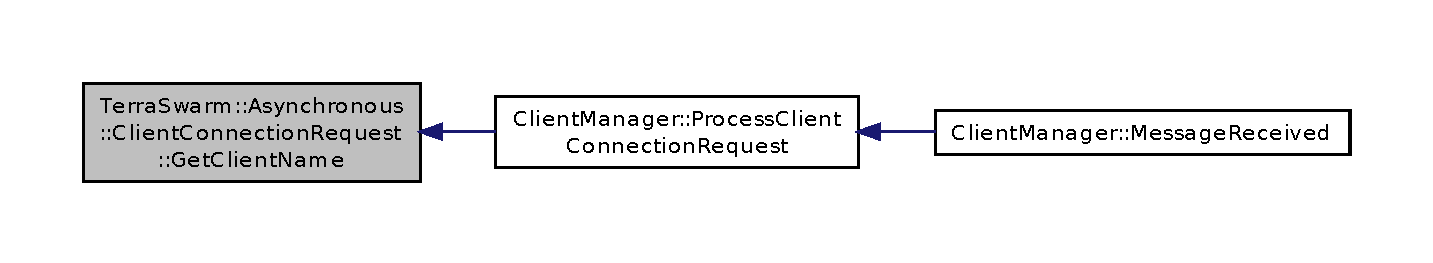
\includegraphics[width=350pt]{class_terra_swarm_1_1_asynchronous_1_1_client_connection_request_a06ce45d6a43bc6e92437a8f6deb5c09a_icgraph}
\end{center}
\end{figure}


\hypertarget{class_terra_swarm_1_1_asynchronous_1_1_client_connection_request_a7325e82c2e6f7f1bb538c287d55ae863}{\index{Terra\-Swarm\-::\-Asynchronous\-::\-Client\-Connection\-Request@{Terra\-Swarm\-::\-Asynchronous\-::\-Client\-Connection\-Request}!Get\-New\-Client\-Connection\-Request@{Get\-New\-Client\-Connection\-Request}}
\index{Get\-New\-Client\-Connection\-Request@{Get\-New\-Client\-Connection\-Request}!TerraSwarm::Asynchronous::ClientConnectionRequest@{Terra\-Swarm\-::\-Asynchronous\-::\-Client\-Connection\-Request}}
\subsubsection[{Get\-New\-Client\-Connection\-Request}]{\setlength{\rightskip}{0pt plus 5cm}{\bf Client\-Connection\-Request} $\ast$ Terra\-Swarm\-::\-Asynchronous\-::\-Client\-Connection\-Request\-::\-Get\-New\-Client\-Connection\-Request (
\begin{DoxyParamCaption}
\item[{const {\bf Message\-Header\-::\-T\-Sender\-Id}}]{sender\-Id, }
\item[{const {\bf Message\-Header\-::\-T\-Receiver\-Id}}]{receiver\-Id, }
\item[{const {\bf T\-Client\-Name} \&}]{client\-Name}
\end{DoxyParamCaption}
)\hspace{0.3cm}{\ttfamily [static]}}}\label{class_terra_swarm_1_1_asynchronous_1_1_client_connection_request_a7325e82c2e6f7f1bb538c287d55ae863}


Definition at line 25 of file Client\-Connection\-Request.\-cpp.



The documentation for this class was generated from the following files\-:\begin{DoxyCompactItemize}
\item 
S2\-Sim/\-Terraswarm\-Library/\hyperlink{_client_connection_request_8h}{Client\-Connection\-Request.\-h}\item 
S2\-Sim/\-Terraswarm\-Library/\hyperlink{_client_connection_request_8cpp}{Client\-Connection\-Request.\-cpp}\end{DoxyCompactItemize}

\hypertarget{class_terra_swarm_1_1_synchronous_1_1_client_connection_request}{\section{Terra\-Swarm\-:\-:Synchronous\-:\-:Client\-Connection\-Request Class Reference}
\label{class_terra_swarm_1_1_synchronous_1_1_client_connection_request}\index{Terra\-Swarm\-::\-Synchronous\-::\-Client\-Connection\-Request@{Terra\-Swarm\-::\-Synchronous\-::\-Client\-Connection\-Request}}
}


This class implements the synchronous client connection request message.  




{\ttfamily \#include $<$Client\-Connection\-Request.\-h$>$}

\subsection*{Public Types}
\begin{DoxyCompactItemize}
\item 
enum \hyperlink{class_terra_swarm_1_1_synchronous_1_1_client_connection_request_a784811f86bbc4a1f1232bdbb579db93d}{Check\-Result\-Values} \{ \hyperlink{class_terra_swarm_1_1_synchronous_1_1_client_connection_request_a784811f86bbc4a1f1232bdbb579db93da20fdb875e0dbe807b95684298bac22bc}{Success} = ( T\-Check\-Result )true, 
\hyperlink{class_terra_swarm_1_1_synchronous_1_1_client_connection_request_a784811f86bbc4a1f1232bdbb579db93da78a023654a74eef1adaae15475a5fa3f}{Fail} = ( T\-Check\-Result )false
 \}
\begin{DoxyCompactList}\small\item\em Defines the values for T\-Check\-Result. \end{DoxyCompactList}\item 
typedef std\-::string \hyperlink{class_terra_swarm_1_1_synchronous_1_1_client_connection_request_a7d85ca6773adf2b3b32cfbff9706f882}{T\-Client\-Name}
\begin{DoxyCompactList}\small\item\em Defines the object name type. \end{DoxyCompactList}\item 
typedef bool \hyperlink{class_terra_swarm_1_1_synchronous_1_1_client_connection_request_af97d7c46396bc29dd8a2628f32a434f2}{T\-Check\-Result}
\begin{DoxyCompactList}\small\item\em Defines the message check result type. \end{DoxyCompactList}\end{DoxyCompactItemize}
\subsection*{Public Member Functions}
\begin{DoxyCompactItemize}
\item 
\hyperlink{class_terra_swarm_1_1_synchronous_1_1_client_connection_request_a810bd205bf787cbdbf931501666d2445}{$\sim$\-Client\-Connection\-Request} (void)
\begin{DoxyCompactList}\small\item\em Deletes the current memory. \end{DoxyCompactList}\item 
\hyperlink{class_terra_swarm_1_1_synchronous_1_1_client_connection_request_af97d7c46396bc29dd8a2628f32a434f2}{T\-Check\-Result} \hyperlink{class_terra_swarm_1_1_synchronous_1_1_client_connection_request_ac50add84d52e10fcaf148444c09e7145}{Check\-Message} (void) const 
\begin{DoxyCompactList}\small\item\em Checks whether the current memory address contains a Client Connection Request message. \end{DoxyCompactList}\item 
\hyperlink{class_terra_swarm_1_1_synchronous_1_1_client_connection_request_a7d85ca6773adf2b3b32cfbff9706f882}{T\-Client\-Name} \hyperlink{class_terra_swarm_1_1_synchronous_1_1_client_connection_request_a94838790aca6aa864fd95b85bddfeaeb}{Get\-Client\-Name} (void) const 
\begin{DoxyCompactList}\small\item\em Returns the object name. \end{DoxyCompactList}\end{DoxyCompactItemize}
\subsection*{Static Public Member Functions}
\begin{DoxyCompactItemize}
\item 
static \hyperlink{class_terra_swarm_1_1_synchronous_1_1_client_connection_request}{Client\-Connection\-Request} $\ast$ \hyperlink{class_terra_swarm_1_1_synchronous_1_1_client_connection_request_a73614eb55926c474741df4d752a34331}{Get\-New\-Client\-Connection\-Request} (const \hyperlink{class_terra_swarm_1_1_message_header_a516b36855e2aad7cfbf8770f1b42784f}{Message\-Header\-::\-T\-Sender\-Id} sender\-Id, const \hyperlink{class_terra_swarm_1_1_message_header_aa3260702b182b6f88ddbdd3416e98df0}{Message\-Header\-::\-T\-Receiver\-Id} receiver\-Id, const \hyperlink{class_terra_swarm_1_1_synchronous_1_1_client_connection_request_a7d85ca6773adf2b3b32cfbff9706f882}{T\-Client\-Name} \&client\-Name)
\begin{DoxyCompactList}\small\item\em This function creates a new Client Connection Request message. \end{DoxyCompactList}\end{DoxyCompactItemize}
\subsection*{Private Types}
\begin{DoxyCompactItemize}
\item 
enum \hyperlink{class_terra_swarm_1_1_synchronous_1_1_client_connection_request_aea4a8b2edd6730c9b592394868d059e3}{Header\-Values} \{ \hyperlink{class_terra_swarm_1_1_synchronous_1_1_client_connection_request_aea4a8b2edd6730c9b592394868d059e3abd99d038acc6de976f899ab9fc50595d}{Message\-Type} = 0x0001, 
\hyperlink{class_terra_swarm_1_1_synchronous_1_1_client_connection_request_aea4a8b2edd6730c9b592394868d059e3a53c5286b4426b73ea18df2b4e03948ff}{Message\-Id} = 0x0004
 \}
\begin{DoxyCompactList}\small\item\em Defines the header values for message recognition. \end{DoxyCompactList}\end{DoxyCompactItemize}
\subsection*{Private Member Functions}
\begin{DoxyCompactItemize}
\item 
\hyperlink{class_terra_swarm_1_1_synchronous_1_1_client_connection_request_a807ffa63107a4e1147eebde79ed61f68}{Client\-Connection\-Request} (void)
\begin{DoxyCompactList}\small\item\em Not used. \end{DoxyCompactList}\end{DoxyCompactItemize}


\subsection{Detailed Description}
This class implements the synchronous client connection request message. 

Definition at line 113 of file Client\-Connection\-Request.\-h.



\subsection{Member Typedef Documentation}
\hypertarget{class_terra_swarm_1_1_synchronous_1_1_client_connection_request_af97d7c46396bc29dd8a2628f32a434f2}{\index{Terra\-Swarm\-::\-Synchronous\-::\-Client\-Connection\-Request@{Terra\-Swarm\-::\-Synchronous\-::\-Client\-Connection\-Request}!T\-Check\-Result@{T\-Check\-Result}}
\index{T\-Check\-Result@{T\-Check\-Result}!TerraSwarm::Synchronous::ClientConnectionRequest@{Terra\-Swarm\-::\-Synchronous\-::\-Client\-Connection\-Request}}
\subsubsection[{T\-Check\-Result}]{\setlength{\rightskip}{0pt plus 5cm}typedef bool {\bf Terra\-Swarm\-::\-Synchronous\-::\-Client\-Connection\-Request\-::\-T\-Check\-Result}}}\label{class_terra_swarm_1_1_synchronous_1_1_client_connection_request_af97d7c46396bc29dd8a2628f32a434f2}


Defines the message check result type. 



Definition at line 134 of file Client\-Connection\-Request.\-h.

\hypertarget{class_terra_swarm_1_1_synchronous_1_1_client_connection_request_a7d85ca6773adf2b3b32cfbff9706f882}{\index{Terra\-Swarm\-::\-Synchronous\-::\-Client\-Connection\-Request@{Terra\-Swarm\-::\-Synchronous\-::\-Client\-Connection\-Request}!T\-Client\-Name@{T\-Client\-Name}}
\index{T\-Client\-Name@{T\-Client\-Name}!TerraSwarm::Synchronous::ClientConnectionRequest@{Terra\-Swarm\-::\-Synchronous\-::\-Client\-Connection\-Request}}
\subsubsection[{T\-Client\-Name}]{\setlength{\rightskip}{0pt plus 5cm}typedef std\-::string {\bf Terra\-Swarm\-::\-Synchronous\-::\-Client\-Connection\-Request\-::\-T\-Client\-Name}}}\label{class_terra_swarm_1_1_synchronous_1_1_client_connection_request_a7d85ca6773adf2b3b32cfbff9706f882}


Defines the object name type. 



Definition at line 129 of file Client\-Connection\-Request.\-h.



\subsection{Member Enumeration Documentation}
\hypertarget{class_terra_swarm_1_1_synchronous_1_1_client_connection_request_a784811f86bbc4a1f1232bdbb579db93d}{\index{Terra\-Swarm\-::\-Synchronous\-::\-Client\-Connection\-Request@{Terra\-Swarm\-::\-Synchronous\-::\-Client\-Connection\-Request}!Check\-Result\-Values@{Check\-Result\-Values}}
\index{Check\-Result\-Values@{Check\-Result\-Values}!TerraSwarm::Synchronous::ClientConnectionRequest@{Terra\-Swarm\-::\-Synchronous\-::\-Client\-Connection\-Request}}
\subsubsection[{Check\-Result\-Values}]{\setlength{\rightskip}{0pt plus 5cm}enum {\bf Terra\-Swarm\-::\-Synchronous\-::\-Client\-Connection\-Request\-::\-Check\-Result\-Values}}}\label{class_terra_swarm_1_1_synchronous_1_1_client_connection_request_a784811f86bbc4a1f1232bdbb579db93d}


Defines the values for T\-Check\-Result. 

\begin{Desc}
\item[Enumerator]\par
\begin{description}
\index{Success@{Success}!Terra\-Swarm\-::\-Synchronous\-::\-Client\-Connection\-Request@{Terra\-Swarm\-::\-Synchronous\-::\-Client\-Connection\-Request}}\index{Terra\-Swarm\-::\-Synchronous\-::\-Client\-Connection\-Request@{Terra\-Swarm\-::\-Synchronous\-::\-Client\-Connection\-Request}!Success@{Success}}\item[{\em 
\hypertarget{class_terra_swarm_1_1_synchronous_1_1_client_connection_request_a784811f86bbc4a1f1232bdbb579db93da20fdb875e0dbe807b95684298bac22bc}{Success}\label{class_terra_swarm_1_1_synchronous_1_1_client_connection_request_a784811f86bbc4a1f1232bdbb579db93da20fdb875e0dbe807b95684298bac22bc}
}]Message is of correct type and id. \index{Fail@{Fail}!Terra\-Swarm\-::\-Synchronous\-::\-Client\-Connection\-Request@{Terra\-Swarm\-::\-Synchronous\-::\-Client\-Connection\-Request}}\index{Terra\-Swarm\-::\-Synchronous\-::\-Client\-Connection\-Request@{Terra\-Swarm\-::\-Synchronous\-::\-Client\-Connection\-Request}!Fail@{Fail}}\item[{\em 
\hypertarget{class_terra_swarm_1_1_synchronous_1_1_client_connection_request_a784811f86bbc4a1f1232bdbb579db93da78a023654a74eef1adaae15475a5fa3f}{Fail}\label{class_terra_swarm_1_1_synchronous_1_1_client_connection_request_a784811f86bbc4a1f1232bdbb579db93da78a023654a74eef1adaae15475a5fa3f}
}]Message has incorrect type or id. \end{description}
\end{Desc}


Definition at line 139 of file Client\-Connection\-Request.\-h.

\hypertarget{class_terra_swarm_1_1_synchronous_1_1_client_connection_request_aea4a8b2edd6730c9b592394868d059e3}{\index{Terra\-Swarm\-::\-Synchronous\-::\-Client\-Connection\-Request@{Terra\-Swarm\-::\-Synchronous\-::\-Client\-Connection\-Request}!Header\-Values@{Header\-Values}}
\index{Header\-Values@{Header\-Values}!TerraSwarm::Synchronous::ClientConnectionRequest@{Terra\-Swarm\-::\-Synchronous\-::\-Client\-Connection\-Request}}
\subsubsection[{Header\-Values}]{\setlength{\rightskip}{0pt plus 5cm}enum {\bf Terra\-Swarm\-::\-Synchronous\-::\-Client\-Connection\-Request\-::\-Header\-Values}\hspace{0.3cm}{\ttfamily [private]}}}\label{class_terra_swarm_1_1_synchronous_1_1_client_connection_request_aea4a8b2edd6730c9b592394868d059e3}


Defines the header values for message recognition. 

\begin{Desc}
\item[Enumerator]\par
\begin{description}
\index{Message\-Type@{Message\-Type}!Terra\-Swarm\-::\-Synchronous\-::\-Client\-Connection\-Request@{Terra\-Swarm\-::\-Synchronous\-::\-Client\-Connection\-Request}}\index{Terra\-Swarm\-::\-Synchronous\-::\-Client\-Connection\-Request@{Terra\-Swarm\-::\-Synchronous\-::\-Client\-Connection\-Request}!Message\-Type@{Message\-Type}}\item[{\em 
\hypertarget{class_terra_swarm_1_1_synchronous_1_1_client_connection_request_aea4a8b2edd6730c9b592394868d059e3abd99d038acc6de976f899ab9fc50595d}{Message\-Type}\label{class_terra_swarm_1_1_synchronous_1_1_client_connection_request_aea4a8b2edd6730c9b592394868d059e3abd99d038acc6de976f899ab9fc50595d}
}]\index{Message\-Id@{Message\-Id}!Terra\-Swarm\-::\-Synchronous\-::\-Client\-Connection\-Request@{Terra\-Swarm\-::\-Synchronous\-::\-Client\-Connection\-Request}}\index{Terra\-Swarm\-::\-Synchronous\-::\-Client\-Connection\-Request@{Terra\-Swarm\-::\-Synchronous\-::\-Client\-Connection\-Request}!Message\-Id@{Message\-Id}}\item[{\em 
\hypertarget{class_terra_swarm_1_1_synchronous_1_1_client_connection_request_aea4a8b2edd6730c9b592394868d059e3a53c5286b4426b73ea18df2b4e03948ff}{Message\-Id}\label{class_terra_swarm_1_1_synchronous_1_1_client_connection_request_aea4a8b2edd6730c9b592394868d059e3a53c5286b4426b73ea18df2b4e03948ff}
}]\end{description}
\end{Desc}


Definition at line 119 of file Client\-Connection\-Request.\-h.



\subsection{Constructor \& Destructor Documentation}
\hypertarget{class_terra_swarm_1_1_synchronous_1_1_client_connection_request_a807ffa63107a4e1147eebde79ed61f68}{\index{Terra\-Swarm\-::\-Synchronous\-::\-Client\-Connection\-Request@{Terra\-Swarm\-::\-Synchronous\-::\-Client\-Connection\-Request}!Client\-Connection\-Request@{Client\-Connection\-Request}}
\index{Client\-Connection\-Request@{Client\-Connection\-Request}!TerraSwarm::Synchronous::ClientConnectionRequest@{Terra\-Swarm\-::\-Synchronous\-::\-Client\-Connection\-Request}}
\subsubsection[{Client\-Connection\-Request}]{\setlength{\rightskip}{0pt plus 5cm}Terra\-Swarm\-::\-Synchronous\-::\-Client\-Connection\-Request\-::\-Client\-Connection\-Request (
\begin{DoxyParamCaption}
\item[{void}]{}
\end{DoxyParamCaption}
)\hspace{0.3cm}{\ttfamily [private]}}}\label{class_terra_swarm_1_1_synchronous_1_1_client_connection_request_a807ffa63107a4e1147eebde79ed61f68}


Not used. 

Made private to force the usage of the static method for creation. 

Definition at line 62 of file Client\-Connection\-Request.\-cpp.

\hypertarget{class_terra_swarm_1_1_synchronous_1_1_client_connection_request_a810bd205bf787cbdbf931501666d2445}{\index{Terra\-Swarm\-::\-Synchronous\-::\-Client\-Connection\-Request@{Terra\-Swarm\-::\-Synchronous\-::\-Client\-Connection\-Request}!$\sim$\-Client\-Connection\-Request@{$\sim$\-Client\-Connection\-Request}}
\index{$\sim$\-Client\-Connection\-Request@{$\sim$\-Client\-Connection\-Request}!TerraSwarm::Synchronous::ClientConnectionRequest@{Terra\-Swarm\-::\-Synchronous\-::\-Client\-Connection\-Request}}
\subsubsection[{$\sim$\-Client\-Connection\-Request}]{\setlength{\rightskip}{0pt plus 5cm}Terra\-Swarm\-::\-Synchronous\-::\-Client\-Connection\-Request\-::$\sim$\-Client\-Connection\-Request (
\begin{DoxyParamCaption}
\item[{void}]{}
\end{DoxyParamCaption}
)}}\label{class_terra_swarm_1_1_synchronous_1_1_client_connection_request_a810bd205bf787cbdbf931501666d2445}


Deletes the current memory. 



Definition at line 66 of file Client\-Connection\-Request.\-cpp.



\subsection{Member Function Documentation}
\hypertarget{class_terra_swarm_1_1_synchronous_1_1_client_connection_request_ac50add84d52e10fcaf148444c09e7145}{\index{Terra\-Swarm\-::\-Synchronous\-::\-Client\-Connection\-Request@{Terra\-Swarm\-::\-Synchronous\-::\-Client\-Connection\-Request}!Check\-Message@{Check\-Message}}
\index{Check\-Message@{Check\-Message}!TerraSwarm::Synchronous::ClientConnectionRequest@{Terra\-Swarm\-::\-Synchronous\-::\-Client\-Connection\-Request}}
\subsubsection[{Check\-Message}]{\setlength{\rightskip}{0pt plus 5cm}{\bf Client\-Connection\-Request\-::\-T\-Check\-Result} Terra\-Swarm\-::\-Synchronous\-::\-Client\-Connection\-Request\-::\-Check\-Message (
\begin{DoxyParamCaption}
\item[{void}]{}
\end{DoxyParamCaption}
) const}}\label{class_terra_swarm_1_1_synchronous_1_1_client_connection_request_ac50add84d52e10fcaf148444c09e7145}


Checks whether the current memory address contains a Client Connection Request message. 

Cast the received memory to the pointer of this class and call this method for checking.

\begin{DoxyReturn}{Returns}
Check result of the memory. 
\end{DoxyReturn}


Definition at line 88 of file Client\-Connection\-Request.\-cpp.

\hypertarget{class_terra_swarm_1_1_synchronous_1_1_client_connection_request_a94838790aca6aa864fd95b85bddfeaeb}{\index{Terra\-Swarm\-::\-Synchronous\-::\-Client\-Connection\-Request@{Terra\-Swarm\-::\-Synchronous\-::\-Client\-Connection\-Request}!Get\-Client\-Name@{Get\-Client\-Name}}
\index{Get\-Client\-Name@{Get\-Client\-Name}!TerraSwarm::Synchronous::ClientConnectionRequest@{Terra\-Swarm\-::\-Synchronous\-::\-Client\-Connection\-Request}}
\subsubsection[{Get\-Client\-Name}]{\setlength{\rightskip}{0pt plus 5cm}{\bf Client\-Connection\-Request\-::\-T\-Client\-Name} Terra\-Swarm\-::\-Synchronous\-::\-Client\-Connection\-Request\-::\-Get\-Client\-Name (
\begin{DoxyParamCaption}
\item[{void}]{}
\end{DoxyParamCaption}
) const}}\label{class_terra_swarm_1_1_synchronous_1_1_client_connection_request_a94838790aca6aa864fd95b85bddfeaeb}


Returns the object name. 

\begin{DoxyReturn}{Returns}
Name of the object within the message. 
\end{DoxyReturn}


Definition at line 99 of file Client\-Connection\-Request.\-cpp.



Here is the caller graph for this function\-:\nopagebreak
\begin{figure}[H]
\begin{center}
\leavevmode
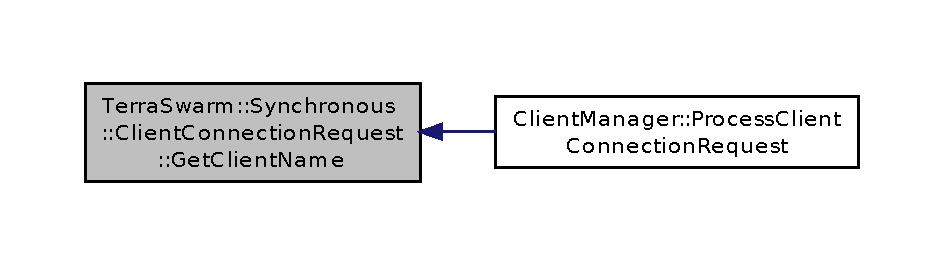
\includegraphics[width=350pt]{class_terra_swarm_1_1_synchronous_1_1_client_connection_request_a94838790aca6aa864fd95b85bddfeaeb_icgraph}
\end{center}
\end{figure}


\hypertarget{class_terra_swarm_1_1_synchronous_1_1_client_connection_request_a73614eb55926c474741df4d752a34331}{\index{Terra\-Swarm\-::\-Synchronous\-::\-Client\-Connection\-Request@{Terra\-Swarm\-::\-Synchronous\-::\-Client\-Connection\-Request}!Get\-New\-Client\-Connection\-Request@{Get\-New\-Client\-Connection\-Request}}
\index{Get\-New\-Client\-Connection\-Request@{Get\-New\-Client\-Connection\-Request}!TerraSwarm::Synchronous::ClientConnectionRequest@{Terra\-Swarm\-::\-Synchronous\-::\-Client\-Connection\-Request}}
\subsubsection[{Get\-New\-Client\-Connection\-Request}]{\setlength{\rightskip}{0pt plus 5cm}{\bf Client\-Connection\-Request} $\ast$ Terra\-Swarm\-::\-Synchronous\-::\-Client\-Connection\-Request\-::\-Get\-New\-Client\-Connection\-Request (
\begin{DoxyParamCaption}
\item[{const {\bf Message\-Header\-::\-T\-Sender\-Id}}]{sender\-Id, }
\item[{const {\bf Message\-Header\-::\-T\-Receiver\-Id}}]{receiver\-Id, }
\item[{const {\bf T\-Client\-Name} \&}]{client\-Name}
\end{DoxyParamCaption}
)\hspace{0.3cm}{\ttfamily [static]}}}\label{class_terra_swarm_1_1_synchronous_1_1_client_connection_request_a73614eb55926c474741df4d752a34331}


This function creates a new Client Connection Request message. 


\begin{DoxyParams}{Parameters}
{\em sender\-Id} & Id of the client. \\
\hline
{\em receiver\-Id} & Id of S2\-Sim. \\
\hline
{\em client\-Name} & Name of the object, the client is representing.\\
\hline
\end{DoxyParams}
\begin{DoxyReturn}{Returns}
A new allocated message. 
\end{DoxyReturn}
\begin{DoxyWarning}{Warning}
The deallocation is user's duty. 
\end{DoxyWarning}


Definition at line 72 of file Client\-Connection\-Request.\-cpp.



The documentation for this class was generated from the following files\-:\begin{DoxyCompactItemize}
\item 
S2\-Sim/\-Terraswarm\-Library/\hyperlink{_client_connection_request_8h}{Client\-Connection\-Request.\-h}\item 
S2\-Sim/\-Terraswarm\-Library/\hyperlink{_client_connection_request_8cpp}{Client\-Connection\-Request.\-cpp}\end{DoxyCompactItemize}

\hypertarget{class_terra_swarm_1_1_asynchronous_1_1_client_connection_response}{\section{Terra\-Swarm\-:\-:Asynchronous\-:\-:Client\-Connection\-Response Class Reference}
\label{class_terra_swarm_1_1_asynchronous_1_1_client_connection_response}\index{Terra\-Swarm\-::\-Asynchronous\-::\-Client\-Connection\-Response@{Terra\-Swarm\-::\-Asynchronous\-::\-Client\-Connection\-Response}}
}


{\ttfamily \#include $<$Client\-Connection\-Response.\-h$>$}

\subsection*{Public Types}
\begin{DoxyCompactItemize}
\item 
enum \hyperlink{class_terra_swarm_1_1_asynchronous_1_1_client_connection_response_a6ca5be4e8bbd731c78f132f1c36513ab}{Check\-Result\-Values} \{ \hyperlink{class_terra_swarm_1_1_asynchronous_1_1_client_connection_response_a6ca5be4e8bbd731c78f132f1c36513abab6f5e3d2684a7900eaf26759bca7985a}{Success} = ( T\-Check\-Result )true, 
\hyperlink{class_terra_swarm_1_1_asynchronous_1_1_client_connection_response_a6ca5be4e8bbd731c78f132f1c36513aba3e6ded9f7aac9629d82cf4c50d232cf0}{Fail} = ( T\-Check\-Result )false
 \}
\item 
enum \hyperlink{class_terra_swarm_1_1_asynchronous_1_1_client_connection_response_a0ebeb46e785ebdd94d1b7e2c9bad80e8}{Request\-Result\-Values} \{ \hyperlink{class_terra_swarm_1_1_asynchronous_1_1_client_connection_response_a0ebeb46e785ebdd94d1b7e2c9bad80e8a81d9cf33ed428b0b13e67f28fc7aca73}{Request\-Accepted} = ( T\-Request\-Result )0x00000000, 
\hyperlink{class_terra_swarm_1_1_asynchronous_1_1_client_connection_response_a0ebeb46e785ebdd94d1b7e2c9bad80e8aea62f4e9889f66d001662d6fa7bea4eb}{Request\-Object\-Id\-Not\-Found} = ( T\-Request\-Result )0x00000001
 \}
\item 
enum \hyperlink{class_terra_swarm_1_1_asynchronous_1_1_client_connection_response_a980f1fa3c9f50c7013f2c2f2d7d6043c}{System\-Mode\-Values} \{ \hyperlink{class_terra_swarm_1_1_asynchronous_1_1_client_connection_response_a980f1fa3c9f50c7013f2c2f2d7d6043ca5d65d9ac052a2eb8917de303ebbeb913}{Simulation\-Mode} = ( T\-System\-Mode )0x0001, 
\hyperlink{class_terra_swarm_1_1_asynchronous_1_1_client_connection_response_a980f1fa3c9f50c7013f2c2f2d7d6043cadc0d1643e730abaef6c00b5cb62005e9}{Real\-Time\-Mode} = ( T\-System\-Mode )0x0002
 \}
\item 
typedef bool \hyperlink{class_terra_swarm_1_1_asynchronous_1_1_client_connection_response_aee00184a039b2aebfcefd9d5b5b71c89}{T\-Check\-Result}
\item 
typedef unsigned int \hyperlink{class_terra_swarm_1_1_asynchronous_1_1_client_connection_response_a55a4d4527b877bde0e74da223157a62a}{T\-Request\-Result}
\item 
typedef unsigned int \hyperlink{class_terra_swarm_1_1_asynchronous_1_1_client_connection_response_ac32ae5e652874b024aae5ed2f816c155}{T\-System\-Time}
\item 
typedef unsigned short \hyperlink{class_terra_swarm_1_1_asynchronous_1_1_client_connection_response_a0780de58d62395a3cce207fe96e43ccc}{T\-Number\-Of\-Clients}
\item 
typedef unsigned short \hyperlink{class_terra_swarm_1_1_asynchronous_1_1_client_connection_response_ac34facba96c97e6897a1abd5ddd09159}{T\-System\-Mode}
\end{DoxyCompactItemize}
\subsection*{Public Member Functions}
\begin{DoxyCompactItemize}
\item 
\hyperlink{class_terra_swarm_1_1_asynchronous_1_1_client_connection_response_ad453032bf556306c0b603340a9e88e51}{$\sim$\-Client\-Connection\-Response} (void)
\item 
\hyperlink{class_terra_swarm_1_1_asynchronous_1_1_client_connection_response_aee00184a039b2aebfcefd9d5b5b71c89}{T\-Check\-Result} \hyperlink{class_terra_swarm_1_1_asynchronous_1_1_client_connection_response_a26dc6c7aa5b7114902a8ea0853d216aa}{Check\-Message} (void) const 
\item 
\hyperlink{class_terra_swarm_1_1_asynchronous_1_1_client_connection_response_a55a4d4527b877bde0e74da223157a62a}{T\-Request\-Result} \hyperlink{class_terra_swarm_1_1_asynchronous_1_1_client_connection_response_a84212711aa29decd7cae02a58b2c2fa9}{Get\-Request\-Result} (void) const 
\item 
\hyperlink{class_terra_swarm_1_1_asynchronous_1_1_client_connection_response_ac32ae5e652874b024aae5ed2f816c155}{T\-System\-Time} \hyperlink{class_terra_swarm_1_1_asynchronous_1_1_client_connection_response_a2126f791ce018128bbf551dd78969a14}{Get\-System\-Time} (void) const 
\item 
\hyperlink{class_terra_swarm_1_1_asynchronous_1_1_client_connection_response_a0780de58d62395a3cce207fe96e43ccc}{T\-Number\-Of\-Clients} \hyperlink{class_terra_swarm_1_1_asynchronous_1_1_client_connection_response_ad261b24429adf40a254d3ede6894d06c}{Get\-Number\-Of\-Clients} (void) const 
\item 
\hyperlink{class_terra_swarm_1_1_asynchronous_1_1_client_connection_response_ac34facba96c97e6897a1abd5ddd09159}{T\-System\-Mode} \hyperlink{class_terra_swarm_1_1_asynchronous_1_1_client_connection_response_a60cb414aaa5b3b7c27c461e1b993b9c5}{Get\-System\-Mode} (void) const 
\end{DoxyCompactItemize}
\subsection*{Static Public Member Functions}
\begin{DoxyCompactItemize}
\item 
static \hyperlink{class_terra_swarm_1_1_asynchronous_1_1_client_connection_response}{Client\-Connection\-Response} $\ast$ \hyperlink{class_terra_swarm_1_1_asynchronous_1_1_client_connection_response_a5ecdefe1ecb557a0086f11f817db793d}{Get\-New\-Client\-Connection\-Response} (const \hyperlink{class_terra_swarm_1_1_message_header_a516b36855e2aad7cfbf8770f1b42784f}{Message\-Header\-::\-T\-Sender\-Id} sender\-Id, const \hyperlink{class_terra_swarm_1_1_message_header_aa3260702b182b6f88ddbdd3416e98df0}{Message\-Header\-::\-T\-Receiver\-Id} receiver\-Id, const \hyperlink{class_terra_swarm_1_1_asynchronous_1_1_client_connection_response_a55a4d4527b877bde0e74da223157a62a}{T\-Request\-Result} request\-Result, const \hyperlink{class_terra_swarm_1_1_asynchronous_1_1_client_connection_response_ac32ae5e652874b024aae5ed2f816c155}{T\-System\-Time} system\-Time, const \hyperlink{class_terra_swarm_1_1_asynchronous_1_1_client_connection_response_a0780de58d62395a3cce207fe96e43ccc}{T\-Number\-Of\-Clients} number\-Of\-Clients, const \hyperlink{class_terra_swarm_1_1_asynchronous_1_1_client_connection_response_ac34facba96c97e6897a1abd5ddd09159}{T\-System\-Mode} system\-Mode)
\item 
static \hyperlink{namespace_terra_swarm_a092e6ec9739175076ae3106783f5c1b6}{T\-Data\-Size} \hyperlink{class_terra_swarm_1_1_asynchronous_1_1_client_connection_response_ac5f405bd7621098cd4ca8d61242168ce}{Get\-Size} (void)
\end{DoxyCompactItemize}
\subsection*{Private Types}
\begin{DoxyCompactItemize}
\item 
enum \hyperlink{class_terra_swarm_1_1_asynchronous_1_1_client_connection_response_a210030e9835d5daaae100ff496cc2b99}{Header\-Values} \{ \hyperlink{class_terra_swarm_1_1_asynchronous_1_1_client_connection_response_a210030e9835d5daaae100ff496cc2b99a1b0238ecfc24737ee8aa6565198b4052}{Message\-Type} = 0x0001, 
\hyperlink{class_terra_swarm_1_1_asynchronous_1_1_client_connection_response_a210030e9835d5daaae100ff496cc2b99ad712a2b73f3d9eff7aafa56e30b11bad}{Message\-Id} = 0x0002
 \}
\item 
enum \hyperlink{class_terra_swarm_1_1_asynchronous_1_1_client_connection_response_a059519ab548bdfbe546b4583c5174fe1}{Field\-Size\-Values} \{ \\*
\hyperlink{class_terra_swarm_1_1_asynchronous_1_1_client_connection_response_a059519ab548bdfbe546b4583c5174fe1ad21e0ac9ec91fa55bf9ba9f4881872cf}{Request\-Result\-Size} = sizeof( T\-Request\-Result ), 
\hyperlink{class_terra_swarm_1_1_asynchronous_1_1_client_connection_response_a059519ab548bdfbe546b4583c5174fe1aebe21ab3228fd3367b5372237080e6af}{System\-Time\-Size} = sizeof( T\-System\-Time ), 
\hyperlink{class_terra_swarm_1_1_asynchronous_1_1_client_connection_response_a059519ab548bdfbe546b4583c5174fe1a2723f340b52e7a61e4ed178a70f167df}{Number\-Of\-Clients\-Size} = sizeof( T\-Number\-Of\-Clients ), 
\hyperlink{class_terra_swarm_1_1_asynchronous_1_1_client_connection_response_a059519ab548bdfbe546b4583c5174fe1a837dd622de291c559f0cdd336d8c4644}{System\-Mode\-Size} = sizeof( T\-System\-Mode ), 
\\*
\hyperlink{class_terra_swarm_1_1_asynchronous_1_1_client_connection_response_a059519ab548bdfbe546b4583c5174fe1a8e2d828f094f9ecb69a26c1eed16a103}{Total\-Size} = ( Request\-Result\-Size + System\-Time\-Size + Number\-Of\-Clients\-Size + System\-Mode\-Size )
 \}
\item 
enum \hyperlink{class_terra_swarm_1_1_asynchronous_1_1_client_connection_response_a696e860584893543721be9624b7114fc}{Field\-Index\-Values} \{ \hyperlink{class_terra_swarm_1_1_asynchronous_1_1_client_connection_response_a696e860584893543721be9624b7114fca29bcb52c78bd4915167362f6f59ce536}{Request\-Result\-Index} = Message\-Header\-:\-:Message\-Header\-Size, 
\hyperlink{class_terra_swarm_1_1_asynchronous_1_1_client_connection_response_a696e860584893543721be9624b7114fca24610af2c75e9f00dd1a1bb759c1bcb8}{System\-Time\-Index} = Request\-Result\-Index + Request\-Result\-Size, 
\hyperlink{class_terra_swarm_1_1_asynchronous_1_1_client_connection_response_a696e860584893543721be9624b7114fca00327ef493fd38258f86303295b076e3}{Number\-Of\-Clients\-Index} = System\-Time\-Index + System\-Time\-Size, 
\hyperlink{class_terra_swarm_1_1_asynchronous_1_1_client_connection_response_a696e860584893543721be9624b7114fcaab080fba23b3393ae7737f430dcfe830}{System\-Mode\-Index} = Number\-Of\-Clients\-Index + Number\-Of\-Clients\-Size
 \}
\item 
typedef \hyperlink{class_terra_swarm_1_1_network_byte_accessor}{Network\-Byte\-Accessor}\\*
$<$ \hyperlink{class_terra_swarm_1_1_asynchronous_1_1_client_connection_response_a696e860584893543721be9624b7114fca29bcb52c78bd4915167362f6f59ce536}{Request\-Result\-Index}, \\*
\hyperlink{class_terra_swarm_1_1_asynchronous_1_1_client_connection_response_a059519ab548bdfbe546b4583c5174fe1ad21e0ac9ec91fa55bf9ba9f4881872cf}{Request\-Result\-Size} $>$ \hyperlink{class_terra_swarm_1_1_asynchronous_1_1_client_connection_response_a43af70d1b67752224dd262c6fdd31a7e}{T\-Request\-Result\-Accessor}
\item 
typedef \hyperlink{class_terra_swarm_1_1_network_byte_accessor}{Network\-Byte\-Accessor}\\*
$<$ \hyperlink{class_terra_swarm_1_1_asynchronous_1_1_client_connection_response_a696e860584893543721be9624b7114fca24610af2c75e9f00dd1a1bb759c1bcb8}{System\-Time\-Index}, \\*
\hyperlink{class_terra_swarm_1_1_asynchronous_1_1_client_connection_response_a059519ab548bdfbe546b4583c5174fe1aebe21ab3228fd3367b5372237080e6af}{System\-Time\-Size} $>$ \hyperlink{class_terra_swarm_1_1_asynchronous_1_1_client_connection_response_a64cb8d4313a5d10fa85b3e0b692764bd}{T\-System\-Time\-Accessor}
\item 
typedef \hyperlink{class_terra_swarm_1_1_network_byte_accessor}{Network\-Byte\-Accessor}\\*
$<$ \hyperlink{class_terra_swarm_1_1_asynchronous_1_1_client_connection_response_a696e860584893543721be9624b7114fca00327ef493fd38258f86303295b076e3}{Number\-Of\-Clients\-Index}, \\*
\hyperlink{class_terra_swarm_1_1_asynchronous_1_1_client_connection_response_a059519ab548bdfbe546b4583c5174fe1a2723f340b52e7a61e4ed178a70f167df}{Number\-Of\-Clients\-Size} $>$ \hyperlink{class_terra_swarm_1_1_asynchronous_1_1_client_connection_response_a6740a3389ab57cb4968a15ecf405fd8e}{T\-Number\-Of\-Clients\-Accessor}
\item 
typedef \hyperlink{class_terra_swarm_1_1_network_byte_accessor}{Network\-Byte\-Accessor}\\*
$<$ \hyperlink{class_terra_swarm_1_1_asynchronous_1_1_client_connection_response_a696e860584893543721be9624b7114fcaab080fba23b3393ae7737f430dcfe830}{System\-Mode\-Index}, \\*
\hyperlink{class_terra_swarm_1_1_asynchronous_1_1_client_connection_response_a059519ab548bdfbe546b4583c5174fe1a837dd622de291c559f0cdd336d8c4644}{System\-Mode\-Size} $>$ \hyperlink{class_terra_swarm_1_1_asynchronous_1_1_client_connection_response_a248ac200307842dee28bd5b5cfec47da}{T\-System\-Mode\-Accessor}
\end{DoxyCompactItemize}
\subsection*{Private Member Functions}
\begin{DoxyCompactItemize}
\item 
\hyperlink{class_terra_swarm_1_1_asynchronous_1_1_client_connection_response_ae1af37cee2cfdc1c258573a5cc679830}{Client\-Connection\-Response} (void)
\end{DoxyCompactItemize}


\subsection{Detailed Description}


Definition at line 19 of file Client\-Connection\-Response.\-h.



\subsection{Member Typedef Documentation}
\hypertarget{class_terra_swarm_1_1_asynchronous_1_1_client_connection_response_aee00184a039b2aebfcefd9d5b5b71c89}{\index{Terra\-Swarm\-::\-Asynchronous\-::\-Client\-Connection\-Response@{Terra\-Swarm\-::\-Asynchronous\-::\-Client\-Connection\-Response}!T\-Check\-Result@{T\-Check\-Result}}
\index{T\-Check\-Result@{T\-Check\-Result}!TerraSwarm::Asynchronous::ClientConnectionResponse@{Terra\-Swarm\-::\-Asynchronous\-::\-Client\-Connection\-Response}}
\subsubsection[{T\-Check\-Result}]{\setlength{\rightskip}{0pt plus 5cm}typedef bool {\bf Terra\-Swarm\-::\-Asynchronous\-::\-Client\-Connection\-Response\-::\-T\-Check\-Result}}}\label{class_terra_swarm_1_1_asynchronous_1_1_client_connection_response_aee00184a039b2aebfcefd9d5b5b71c89}


Definition at line 29 of file Client\-Connection\-Response.\-h.

\hypertarget{class_terra_swarm_1_1_asynchronous_1_1_client_connection_response_a0780de58d62395a3cce207fe96e43ccc}{\index{Terra\-Swarm\-::\-Asynchronous\-::\-Client\-Connection\-Response@{Terra\-Swarm\-::\-Asynchronous\-::\-Client\-Connection\-Response}!T\-Number\-Of\-Clients@{T\-Number\-Of\-Clients}}
\index{T\-Number\-Of\-Clients@{T\-Number\-Of\-Clients}!TerraSwarm::Asynchronous::ClientConnectionResponse@{Terra\-Swarm\-::\-Asynchronous\-::\-Client\-Connection\-Response}}
\subsubsection[{T\-Number\-Of\-Clients}]{\setlength{\rightskip}{0pt plus 5cm}typedef unsigned short {\bf Terra\-Swarm\-::\-Asynchronous\-::\-Client\-Connection\-Response\-::\-T\-Number\-Of\-Clients}}}\label{class_terra_swarm_1_1_asynchronous_1_1_client_connection_response_a0780de58d62395a3cce207fe96e43ccc}


Definition at line 44 of file Client\-Connection\-Response.\-h.

\hypertarget{class_terra_swarm_1_1_asynchronous_1_1_client_connection_response_a6740a3389ab57cb4968a15ecf405fd8e}{\index{Terra\-Swarm\-::\-Asynchronous\-::\-Client\-Connection\-Response@{Terra\-Swarm\-::\-Asynchronous\-::\-Client\-Connection\-Response}!T\-Number\-Of\-Clients\-Accessor@{T\-Number\-Of\-Clients\-Accessor}}
\index{T\-Number\-Of\-Clients\-Accessor@{T\-Number\-Of\-Clients\-Accessor}!TerraSwarm::Asynchronous::ClientConnectionResponse@{Terra\-Swarm\-::\-Asynchronous\-::\-Client\-Connection\-Response}}
\subsubsection[{T\-Number\-Of\-Clients\-Accessor}]{\setlength{\rightskip}{0pt plus 5cm}typedef {\bf Network\-Byte\-Accessor}$<${\bf Number\-Of\-Clients\-Index}, {\bf Number\-Of\-Clients\-Size}$>$ {\bf Terra\-Swarm\-::\-Asynchronous\-::\-Client\-Connection\-Response\-::\-T\-Number\-Of\-Clients\-Accessor}\hspace{0.3cm}{\ttfamily [private]}}}\label{class_terra_swarm_1_1_asynchronous_1_1_client_connection_response_a6740a3389ab57cb4968a15ecf405fd8e}


Definition at line 72 of file Client\-Connection\-Response.\-h.

\hypertarget{class_terra_swarm_1_1_asynchronous_1_1_client_connection_response_a55a4d4527b877bde0e74da223157a62a}{\index{Terra\-Swarm\-::\-Asynchronous\-::\-Client\-Connection\-Response@{Terra\-Swarm\-::\-Asynchronous\-::\-Client\-Connection\-Response}!T\-Request\-Result@{T\-Request\-Result}}
\index{T\-Request\-Result@{T\-Request\-Result}!TerraSwarm::Asynchronous::ClientConnectionResponse@{Terra\-Swarm\-::\-Asynchronous\-::\-Client\-Connection\-Response}}
\subsubsection[{T\-Request\-Result}]{\setlength{\rightskip}{0pt plus 5cm}typedef unsigned int {\bf Terra\-Swarm\-::\-Asynchronous\-::\-Client\-Connection\-Response\-::\-T\-Request\-Result}}}\label{class_terra_swarm_1_1_asynchronous_1_1_client_connection_response_a55a4d4527b877bde0e74da223157a62a}


Definition at line 36 of file Client\-Connection\-Response.\-h.

\hypertarget{class_terra_swarm_1_1_asynchronous_1_1_client_connection_response_a43af70d1b67752224dd262c6fdd31a7e}{\index{Terra\-Swarm\-::\-Asynchronous\-::\-Client\-Connection\-Response@{Terra\-Swarm\-::\-Asynchronous\-::\-Client\-Connection\-Response}!T\-Request\-Result\-Accessor@{T\-Request\-Result\-Accessor}}
\index{T\-Request\-Result\-Accessor@{T\-Request\-Result\-Accessor}!TerraSwarm::Asynchronous::ClientConnectionResponse@{Terra\-Swarm\-::\-Asynchronous\-::\-Client\-Connection\-Response}}
\subsubsection[{T\-Request\-Result\-Accessor}]{\setlength{\rightskip}{0pt plus 5cm}typedef {\bf Network\-Byte\-Accessor}$<${\bf Request\-Result\-Index}, {\bf Request\-Result\-Size}$>$ {\bf Terra\-Swarm\-::\-Asynchronous\-::\-Client\-Connection\-Response\-::\-T\-Request\-Result\-Accessor}\hspace{0.3cm}{\ttfamily [private]}}}\label{class_terra_swarm_1_1_asynchronous_1_1_client_connection_response_a43af70d1b67752224dd262c6fdd31a7e}


Definition at line 70 of file Client\-Connection\-Response.\-h.

\hypertarget{class_terra_swarm_1_1_asynchronous_1_1_client_connection_response_ac34facba96c97e6897a1abd5ddd09159}{\index{Terra\-Swarm\-::\-Asynchronous\-::\-Client\-Connection\-Response@{Terra\-Swarm\-::\-Asynchronous\-::\-Client\-Connection\-Response}!T\-System\-Mode@{T\-System\-Mode}}
\index{T\-System\-Mode@{T\-System\-Mode}!TerraSwarm::Asynchronous::ClientConnectionResponse@{Terra\-Swarm\-::\-Asynchronous\-::\-Client\-Connection\-Response}}
\subsubsection[{T\-System\-Mode}]{\setlength{\rightskip}{0pt plus 5cm}typedef unsigned short {\bf Terra\-Swarm\-::\-Asynchronous\-::\-Client\-Connection\-Response\-::\-T\-System\-Mode}}}\label{class_terra_swarm_1_1_asynchronous_1_1_client_connection_response_ac34facba96c97e6897a1abd5ddd09159}


Definition at line 45 of file Client\-Connection\-Response.\-h.

\hypertarget{class_terra_swarm_1_1_asynchronous_1_1_client_connection_response_a248ac200307842dee28bd5b5cfec47da}{\index{Terra\-Swarm\-::\-Asynchronous\-::\-Client\-Connection\-Response@{Terra\-Swarm\-::\-Asynchronous\-::\-Client\-Connection\-Response}!T\-System\-Mode\-Accessor@{T\-System\-Mode\-Accessor}}
\index{T\-System\-Mode\-Accessor@{T\-System\-Mode\-Accessor}!TerraSwarm::Asynchronous::ClientConnectionResponse@{Terra\-Swarm\-::\-Asynchronous\-::\-Client\-Connection\-Response}}
\subsubsection[{T\-System\-Mode\-Accessor}]{\setlength{\rightskip}{0pt plus 5cm}typedef {\bf Network\-Byte\-Accessor}$<${\bf System\-Mode\-Index}, {\bf System\-Mode\-Size}$>$ {\bf Terra\-Swarm\-::\-Asynchronous\-::\-Client\-Connection\-Response\-::\-T\-System\-Mode\-Accessor}\hspace{0.3cm}{\ttfamily [private]}}}\label{class_terra_swarm_1_1_asynchronous_1_1_client_connection_response_a248ac200307842dee28bd5b5cfec47da}


Definition at line 73 of file Client\-Connection\-Response.\-h.

\hypertarget{class_terra_swarm_1_1_asynchronous_1_1_client_connection_response_ac32ae5e652874b024aae5ed2f816c155}{\index{Terra\-Swarm\-::\-Asynchronous\-::\-Client\-Connection\-Response@{Terra\-Swarm\-::\-Asynchronous\-::\-Client\-Connection\-Response}!T\-System\-Time@{T\-System\-Time}}
\index{T\-System\-Time@{T\-System\-Time}!TerraSwarm::Asynchronous::ClientConnectionResponse@{Terra\-Swarm\-::\-Asynchronous\-::\-Client\-Connection\-Response}}
\subsubsection[{T\-System\-Time}]{\setlength{\rightskip}{0pt plus 5cm}typedef unsigned int {\bf Terra\-Swarm\-::\-Asynchronous\-::\-Client\-Connection\-Response\-::\-T\-System\-Time}}}\label{class_terra_swarm_1_1_asynchronous_1_1_client_connection_response_ac32ae5e652874b024aae5ed2f816c155}


Definition at line 43 of file Client\-Connection\-Response.\-h.

\hypertarget{class_terra_swarm_1_1_asynchronous_1_1_client_connection_response_a64cb8d4313a5d10fa85b3e0b692764bd}{\index{Terra\-Swarm\-::\-Asynchronous\-::\-Client\-Connection\-Response@{Terra\-Swarm\-::\-Asynchronous\-::\-Client\-Connection\-Response}!T\-System\-Time\-Accessor@{T\-System\-Time\-Accessor}}
\index{T\-System\-Time\-Accessor@{T\-System\-Time\-Accessor}!TerraSwarm::Asynchronous::ClientConnectionResponse@{Terra\-Swarm\-::\-Asynchronous\-::\-Client\-Connection\-Response}}
\subsubsection[{T\-System\-Time\-Accessor}]{\setlength{\rightskip}{0pt plus 5cm}typedef {\bf Network\-Byte\-Accessor}$<${\bf System\-Time\-Index}, {\bf System\-Time\-Size}$>$ {\bf Terra\-Swarm\-::\-Asynchronous\-::\-Client\-Connection\-Response\-::\-T\-System\-Time\-Accessor}\hspace{0.3cm}{\ttfamily [private]}}}\label{class_terra_swarm_1_1_asynchronous_1_1_client_connection_response_a64cb8d4313a5d10fa85b3e0b692764bd}


Definition at line 71 of file Client\-Connection\-Response.\-h.



\subsection{Member Enumeration Documentation}
\hypertarget{class_terra_swarm_1_1_asynchronous_1_1_client_connection_response_a6ca5be4e8bbd731c78f132f1c36513ab}{\index{Terra\-Swarm\-::\-Asynchronous\-::\-Client\-Connection\-Response@{Terra\-Swarm\-::\-Asynchronous\-::\-Client\-Connection\-Response}!Check\-Result\-Values@{Check\-Result\-Values}}
\index{Check\-Result\-Values@{Check\-Result\-Values}!TerraSwarm::Asynchronous::ClientConnectionResponse@{Terra\-Swarm\-::\-Asynchronous\-::\-Client\-Connection\-Response}}
\subsubsection[{Check\-Result\-Values}]{\setlength{\rightskip}{0pt plus 5cm}enum {\bf Terra\-Swarm\-::\-Asynchronous\-::\-Client\-Connection\-Response\-::\-Check\-Result\-Values}}}\label{class_terra_swarm_1_1_asynchronous_1_1_client_connection_response_a6ca5be4e8bbd731c78f132f1c36513ab}
\begin{Desc}
\item[Enumerator]\par
\begin{description}
\index{Success@{Success}!Terra\-Swarm\-::\-Asynchronous\-::\-Client\-Connection\-Response@{Terra\-Swarm\-::\-Asynchronous\-::\-Client\-Connection\-Response}}\index{Terra\-Swarm\-::\-Asynchronous\-::\-Client\-Connection\-Response@{Terra\-Swarm\-::\-Asynchronous\-::\-Client\-Connection\-Response}!Success@{Success}}\item[{\em 
\hypertarget{class_terra_swarm_1_1_asynchronous_1_1_client_connection_response_a6ca5be4e8bbd731c78f132f1c36513abab6f5e3d2684a7900eaf26759bca7985a}{Success}\label{class_terra_swarm_1_1_asynchronous_1_1_client_connection_response_a6ca5be4e8bbd731c78f132f1c36513abab6f5e3d2684a7900eaf26759bca7985a}
}]\index{Fail@{Fail}!Terra\-Swarm\-::\-Asynchronous\-::\-Client\-Connection\-Response@{Terra\-Swarm\-::\-Asynchronous\-::\-Client\-Connection\-Response}}\index{Terra\-Swarm\-::\-Asynchronous\-::\-Client\-Connection\-Response@{Terra\-Swarm\-::\-Asynchronous\-::\-Client\-Connection\-Response}!Fail@{Fail}}\item[{\em 
\hypertarget{class_terra_swarm_1_1_asynchronous_1_1_client_connection_response_a6ca5be4e8bbd731c78f132f1c36513aba3e6ded9f7aac9629d82cf4c50d232cf0}{Fail}\label{class_terra_swarm_1_1_asynchronous_1_1_client_connection_response_a6ca5be4e8bbd731c78f132f1c36513aba3e6ded9f7aac9629d82cf4c50d232cf0}
}]\end{description}
\end{Desc}


Definition at line 30 of file Client\-Connection\-Response.\-h.

\hypertarget{class_terra_swarm_1_1_asynchronous_1_1_client_connection_response_a696e860584893543721be9624b7114fc}{\index{Terra\-Swarm\-::\-Asynchronous\-::\-Client\-Connection\-Response@{Terra\-Swarm\-::\-Asynchronous\-::\-Client\-Connection\-Response}!Field\-Index\-Values@{Field\-Index\-Values}}
\index{Field\-Index\-Values@{Field\-Index\-Values}!TerraSwarm::Asynchronous::ClientConnectionResponse@{Terra\-Swarm\-::\-Asynchronous\-::\-Client\-Connection\-Response}}
\subsubsection[{Field\-Index\-Values}]{\setlength{\rightskip}{0pt plus 5cm}enum {\bf Terra\-Swarm\-::\-Asynchronous\-::\-Client\-Connection\-Response\-::\-Field\-Index\-Values}\hspace{0.3cm}{\ttfamily [private]}}}\label{class_terra_swarm_1_1_asynchronous_1_1_client_connection_response_a696e860584893543721be9624b7114fc}
\begin{Desc}
\item[Enumerator]\par
\begin{description}
\index{Request\-Result\-Index@{Request\-Result\-Index}!Terra\-Swarm\-::\-Asynchronous\-::\-Client\-Connection\-Response@{Terra\-Swarm\-::\-Asynchronous\-::\-Client\-Connection\-Response}}\index{Terra\-Swarm\-::\-Asynchronous\-::\-Client\-Connection\-Response@{Terra\-Swarm\-::\-Asynchronous\-::\-Client\-Connection\-Response}!Request\-Result\-Index@{Request\-Result\-Index}}\item[{\em 
\hypertarget{class_terra_swarm_1_1_asynchronous_1_1_client_connection_response_a696e860584893543721be9624b7114fca29bcb52c78bd4915167362f6f59ce536}{Request\-Result\-Index}\label{class_terra_swarm_1_1_asynchronous_1_1_client_connection_response_a696e860584893543721be9624b7114fca29bcb52c78bd4915167362f6f59ce536}
}]\index{System\-Time\-Index@{System\-Time\-Index}!Terra\-Swarm\-::\-Asynchronous\-::\-Client\-Connection\-Response@{Terra\-Swarm\-::\-Asynchronous\-::\-Client\-Connection\-Response}}\index{Terra\-Swarm\-::\-Asynchronous\-::\-Client\-Connection\-Response@{Terra\-Swarm\-::\-Asynchronous\-::\-Client\-Connection\-Response}!System\-Time\-Index@{System\-Time\-Index}}\item[{\em 
\hypertarget{class_terra_swarm_1_1_asynchronous_1_1_client_connection_response_a696e860584893543721be9624b7114fca24610af2c75e9f00dd1a1bb759c1bcb8}{System\-Time\-Index}\label{class_terra_swarm_1_1_asynchronous_1_1_client_connection_response_a696e860584893543721be9624b7114fca24610af2c75e9f00dd1a1bb759c1bcb8}
}]\index{Number\-Of\-Clients\-Index@{Number\-Of\-Clients\-Index}!Terra\-Swarm\-::\-Asynchronous\-::\-Client\-Connection\-Response@{Terra\-Swarm\-::\-Asynchronous\-::\-Client\-Connection\-Response}}\index{Terra\-Swarm\-::\-Asynchronous\-::\-Client\-Connection\-Response@{Terra\-Swarm\-::\-Asynchronous\-::\-Client\-Connection\-Response}!Number\-Of\-Clients\-Index@{Number\-Of\-Clients\-Index}}\item[{\em 
\hypertarget{class_terra_swarm_1_1_asynchronous_1_1_client_connection_response_a696e860584893543721be9624b7114fca00327ef493fd38258f86303295b076e3}{Number\-Of\-Clients\-Index}\label{class_terra_swarm_1_1_asynchronous_1_1_client_connection_response_a696e860584893543721be9624b7114fca00327ef493fd38258f86303295b076e3}
}]\index{System\-Mode\-Index@{System\-Mode\-Index}!Terra\-Swarm\-::\-Asynchronous\-::\-Client\-Connection\-Response@{Terra\-Swarm\-::\-Asynchronous\-::\-Client\-Connection\-Response}}\index{Terra\-Swarm\-::\-Asynchronous\-::\-Client\-Connection\-Response@{Terra\-Swarm\-::\-Asynchronous\-::\-Client\-Connection\-Response}!System\-Mode\-Index@{System\-Mode\-Index}}\item[{\em 
\hypertarget{class_terra_swarm_1_1_asynchronous_1_1_client_connection_response_a696e860584893543721be9624b7114fcaab080fba23b3393ae7737f430dcfe830}{System\-Mode\-Index}\label{class_terra_swarm_1_1_asynchronous_1_1_client_connection_response_a696e860584893543721be9624b7114fcaab080fba23b3393ae7737f430dcfe830}
}]\end{description}
\end{Desc}


Definition at line 62 of file Client\-Connection\-Response.\-h.

\hypertarget{class_terra_swarm_1_1_asynchronous_1_1_client_connection_response_a059519ab548bdfbe546b4583c5174fe1}{\index{Terra\-Swarm\-::\-Asynchronous\-::\-Client\-Connection\-Response@{Terra\-Swarm\-::\-Asynchronous\-::\-Client\-Connection\-Response}!Field\-Size\-Values@{Field\-Size\-Values}}
\index{Field\-Size\-Values@{Field\-Size\-Values}!TerraSwarm::Asynchronous::ClientConnectionResponse@{Terra\-Swarm\-::\-Asynchronous\-::\-Client\-Connection\-Response}}
\subsubsection[{Field\-Size\-Values}]{\setlength{\rightskip}{0pt plus 5cm}enum {\bf Terra\-Swarm\-::\-Asynchronous\-::\-Client\-Connection\-Response\-::\-Field\-Size\-Values}\hspace{0.3cm}{\ttfamily [private]}}}\label{class_terra_swarm_1_1_asynchronous_1_1_client_connection_response_a059519ab548bdfbe546b4583c5174fe1}
\begin{Desc}
\item[Enumerator]\par
\begin{description}
\index{Request\-Result\-Size@{Request\-Result\-Size}!Terra\-Swarm\-::\-Asynchronous\-::\-Client\-Connection\-Response@{Terra\-Swarm\-::\-Asynchronous\-::\-Client\-Connection\-Response}}\index{Terra\-Swarm\-::\-Asynchronous\-::\-Client\-Connection\-Response@{Terra\-Swarm\-::\-Asynchronous\-::\-Client\-Connection\-Response}!Request\-Result\-Size@{Request\-Result\-Size}}\item[{\em 
\hypertarget{class_terra_swarm_1_1_asynchronous_1_1_client_connection_response_a059519ab548bdfbe546b4583c5174fe1ad21e0ac9ec91fa55bf9ba9f4881872cf}{Request\-Result\-Size}\label{class_terra_swarm_1_1_asynchronous_1_1_client_connection_response_a059519ab548bdfbe546b4583c5174fe1ad21e0ac9ec91fa55bf9ba9f4881872cf}
}]\index{System\-Time\-Size@{System\-Time\-Size}!Terra\-Swarm\-::\-Asynchronous\-::\-Client\-Connection\-Response@{Terra\-Swarm\-::\-Asynchronous\-::\-Client\-Connection\-Response}}\index{Terra\-Swarm\-::\-Asynchronous\-::\-Client\-Connection\-Response@{Terra\-Swarm\-::\-Asynchronous\-::\-Client\-Connection\-Response}!System\-Time\-Size@{System\-Time\-Size}}\item[{\em 
\hypertarget{class_terra_swarm_1_1_asynchronous_1_1_client_connection_response_a059519ab548bdfbe546b4583c5174fe1aebe21ab3228fd3367b5372237080e6af}{System\-Time\-Size}\label{class_terra_swarm_1_1_asynchronous_1_1_client_connection_response_a059519ab548bdfbe546b4583c5174fe1aebe21ab3228fd3367b5372237080e6af}
}]\index{Number\-Of\-Clients\-Size@{Number\-Of\-Clients\-Size}!Terra\-Swarm\-::\-Asynchronous\-::\-Client\-Connection\-Response@{Terra\-Swarm\-::\-Asynchronous\-::\-Client\-Connection\-Response}}\index{Terra\-Swarm\-::\-Asynchronous\-::\-Client\-Connection\-Response@{Terra\-Swarm\-::\-Asynchronous\-::\-Client\-Connection\-Response}!Number\-Of\-Clients\-Size@{Number\-Of\-Clients\-Size}}\item[{\em 
\hypertarget{class_terra_swarm_1_1_asynchronous_1_1_client_connection_response_a059519ab548bdfbe546b4583c5174fe1a2723f340b52e7a61e4ed178a70f167df}{Number\-Of\-Clients\-Size}\label{class_terra_swarm_1_1_asynchronous_1_1_client_connection_response_a059519ab548bdfbe546b4583c5174fe1a2723f340b52e7a61e4ed178a70f167df}
}]\index{System\-Mode\-Size@{System\-Mode\-Size}!Terra\-Swarm\-::\-Asynchronous\-::\-Client\-Connection\-Response@{Terra\-Swarm\-::\-Asynchronous\-::\-Client\-Connection\-Response}}\index{Terra\-Swarm\-::\-Asynchronous\-::\-Client\-Connection\-Response@{Terra\-Swarm\-::\-Asynchronous\-::\-Client\-Connection\-Response}!System\-Mode\-Size@{System\-Mode\-Size}}\item[{\em 
\hypertarget{class_terra_swarm_1_1_asynchronous_1_1_client_connection_response_a059519ab548bdfbe546b4583c5174fe1a837dd622de291c559f0cdd336d8c4644}{System\-Mode\-Size}\label{class_terra_swarm_1_1_asynchronous_1_1_client_connection_response_a059519ab548bdfbe546b4583c5174fe1a837dd622de291c559f0cdd336d8c4644}
}]\index{Total\-Size@{Total\-Size}!Terra\-Swarm\-::\-Asynchronous\-::\-Client\-Connection\-Response@{Terra\-Swarm\-::\-Asynchronous\-::\-Client\-Connection\-Response}}\index{Terra\-Swarm\-::\-Asynchronous\-::\-Client\-Connection\-Response@{Terra\-Swarm\-::\-Asynchronous\-::\-Client\-Connection\-Response}!Total\-Size@{Total\-Size}}\item[{\em 
\hypertarget{class_terra_swarm_1_1_asynchronous_1_1_client_connection_response_a059519ab548bdfbe546b4583c5174fe1a8e2d828f094f9ecb69a26c1eed16a103}{Total\-Size}\label{class_terra_swarm_1_1_asynchronous_1_1_client_connection_response_a059519ab548bdfbe546b4583c5174fe1a8e2d828f094f9ecb69a26c1eed16a103}
}]\end{description}
\end{Desc}


Definition at line 53 of file Client\-Connection\-Response.\-h.

\hypertarget{class_terra_swarm_1_1_asynchronous_1_1_client_connection_response_a210030e9835d5daaae100ff496cc2b99}{\index{Terra\-Swarm\-::\-Asynchronous\-::\-Client\-Connection\-Response@{Terra\-Swarm\-::\-Asynchronous\-::\-Client\-Connection\-Response}!Header\-Values@{Header\-Values}}
\index{Header\-Values@{Header\-Values}!TerraSwarm::Asynchronous::ClientConnectionResponse@{Terra\-Swarm\-::\-Asynchronous\-::\-Client\-Connection\-Response}}
\subsubsection[{Header\-Values}]{\setlength{\rightskip}{0pt plus 5cm}enum {\bf Terra\-Swarm\-::\-Asynchronous\-::\-Client\-Connection\-Response\-::\-Header\-Values}\hspace{0.3cm}{\ttfamily [private]}}}\label{class_terra_swarm_1_1_asynchronous_1_1_client_connection_response_a210030e9835d5daaae100ff496cc2b99}
\begin{Desc}
\item[Enumerator]\par
\begin{description}
\index{Message\-Type@{Message\-Type}!Terra\-Swarm\-::\-Asynchronous\-::\-Client\-Connection\-Response@{Terra\-Swarm\-::\-Asynchronous\-::\-Client\-Connection\-Response}}\index{Terra\-Swarm\-::\-Asynchronous\-::\-Client\-Connection\-Response@{Terra\-Swarm\-::\-Asynchronous\-::\-Client\-Connection\-Response}!Message\-Type@{Message\-Type}}\item[{\em 
\hypertarget{class_terra_swarm_1_1_asynchronous_1_1_client_connection_response_a210030e9835d5daaae100ff496cc2b99a1b0238ecfc24737ee8aa6565198b4052}{Message\-Type}\label{class_terra_swarm_1_1_asynchronous_1_1_client_connection_response_a210030e9835d5daaae100ff496cc2b99a1b0238ecfc24737ee8aa6565198b4052}
}]\index{Message\-Id@{Message\-Id}!Terra\-Swarm\-::\-Asynchronous\-::\-Client\-Connection\-Response@{Terra\-Swarm\-::\-Asynchronous\-::\-Client\-Connection\-Response}}\index{Terra\-Swarm\-::\-Asynchronous\-::\-Client\-Connection\-Response@{Terra\-Swarm\-::\-Asynchronous\-::\-Client\-Connection\-Response}!Message\-Id@{Message\-Id}}\item[{\em 
\hypertarget{class_terra_swarm_1_1_asynchronous_1_1_client_connection_response_a210030e9835d5daaae100ff496cc2b99ad712a2b73f3d9eff7aafa56e30b11bad}{Message\-Id}\label{class_terra_swarm_1_1_asynchronous_1_1_client_connection_response_a210030e9835d5daaae100ff496cc2b99ad712a2b73f3d9eff7aafa56e30b11bad}
}]\end{description}
\end{Desc}


Definition at line 22 of file Client\-Connection\-Response.\-h.

\hypertarget{class_terra_swarm_1_1_asynchronous_1_1_client_connection_response_a0ebeb46e785ebdd94d1b7e2c9bad80e8}{\index{Terra\-Swarm\-::\-Asynchronous\-::\-Client\-Connection\-Response@{Terra\-Swarm\-::\-Asynchronous\-::\-Client\-Connection\-Response}!Request\-Result\-Values@{Request\-Result\-Values}}
\index{Request\-Result\-Values@{Request\-Result\-Values}!TerraSwarm::Asynchronous::ClientConnectionResponse@{Terra\-Swarm\-::\-Asynchronous\-::\-Client\-Connection\-Response}}
\subsubsection[{Request\-Result\-Values}]{\setlength{\rightskip}{0pt plus 5cm}enum {\bf Terra\-Swarm\-::\-Asynchronous\-::\-Client\-Connection\-Response\-::\-Request\-Result\-Values}}}\label{class_terra_swarm_1_1_asynchronous_1_1_client_connection_response_a0ebeb46e785ebdd94d1b7e2c9bad80e8}
\begin{Desc}
\item[Enumerator]\par
\begin{description}
\index{Request\-Accepted@{Request\-Accepted}!Terra\-Swarm\-::\-Asynchronous\-::\-Client\-Connection\-Response@{Terra\-Swarm\-::\-Asynchronous\-::\-Client\-Connection\-Response}}\index{Terra\-Swarm\-::\-Asynchronous\-::\-Client\-Connection\-Response@{Terra\-Swarm\-::\-Asynchronous\-::\-Client\-Connection\-Response}!Request\-Accepted@{Request\-Accepted}}\item[{\em 
\hypertarget{class_terra_swarm_1_1_asynchronous_1_1_client_connection_response_a0ebeb46e785ebdd94d1b7e2c9bad80e8a81d9cf33ed428b0b13e67f28fc7aca73}{Request\-Accepted}\label{class_terra_swarm_1_1_asynchronous_1_1_client_connection_response_a0ebeb46e785ebdd94d1b7e2c9bad80e8a81d9cf33ed428b0b13e67f28fc7aca73}
}]\index{Request\-Object\-Id\-Not\-Found@{Request\-Object\-Id\-Not\-Found}!Terra\-Swarm\-::\-Asynchronous\-::\-Client\-Connection\-Response@{Terra\-Swarm\-::\-Asynchronous\-::\-Client\-Connection\-Response}}\index{Terra\-Swarm\-::\-Asynchronous\-::\-Client\-Connection\-Response@{Terra\-Swarm\-::\-Asynchronous\-::\-Client\-Connection\-Response}!Request\-Object\-Id\-Not\-Found@{Request\-Object\-Id\-Not\-Found}}\item[{\em 
\hypertarget{class_terra_swarm_1_1_asynchronous_1_1_client_connection_response_a0ebeb46e785ebdd94d1b7e2c9bad80e8aea62f4e9889f66d001662d6fa7bea4eb}{Request\-Object\-Id\-Not\-Found}\label{class_terra_swarm_1_1_asynchronous_1_1_client_connection_response_a0ebeb46e785ebdd94d1b7e2c9bad80e8aea62f4e9889f66d001662d6fa7bea4eb}
}]\end{description}
\end{Desc}


Definition at line 37 of file Client\-Connection\-Response.\-h.

\hypertarget{class_terra_swarm_1_1_asynchronous_1_1_client_connection_response_a980f1fa3c9f50c7013f2c2f2d7d6043c}{\index{Terra\-Swarm\-::\-Asynchronous\-::\-Client\-Connection\-Response@{Terra\-Swarm\-::\-Asynchronous\-::\-Client\-Connection\-Response}!System\-Mode\-Values@{System\-Mode\-Values}}
\index{System\-Mode\-Values@{System\-Mode\-Values}!TerraSwarm::Asynchronous::ClientConnectionResponse@{Terra\-Swarm\-::\-Asynchronous\-::\-Client\-Connection\-Response}}
\subsubsection[{System\-Mode\-Values}]{\setlength{\rightskip}{0pt plus 5cm}enum {\bf Terra\-Swarm\-::\-Asynchronous\-::\-Client\-Connection\-Response\-::\-System\-Mode\-Values}}}\label{class_terra_swarm_1_1_asynchronous_1_1_client_connection_response_a980f1fa3c9f50c7013f2c2f2d7d6043c}
\begin{Desc}
\item[Enumerator]\par
\begin{description}
\index{Simulation\-Mode@{Simulation\-Mode}!Terra\-Swarm\-::\-Asynchronous\-::\-Client\-Connection\-Response@{Terra\-Swarm\-::\-Asynchronous\-::\-Client\-Connection\-Response}}\index{Terra\-Swarm\-::\-Asynchronous\-::\-Client\-Connection\-Response@{Terra\-Swarm\-::\-Asynchronous\-::\-Client\-Connection\-Response}!Simulation\-Mode@{Simulation\-Mode}}\item[{\em 
\hypertarget{class_terra_swarm_1_1_asynchronous_1_1_client_connection_response_a980f1fa3c9f50c7013f2c2f2d7d6043ca5d65d9ac052a2eb8917de303ebbeb913}{Simulation\-Mode}\label{class_terra_swarm_1_1_asynchronous_1_1_client_connection_response_a980f1fa3c9f50c7013f2c2f2d7d6043ca5d65d9ac052a2eb8917de303ebbeb913}
}]\index{Real\-Time\-Mode@{Real\-Time\-Mode}!Terra\-Swarm\-::\-Asynchronous\-::\-Client\-Connection\-Response@{Terra\-Swarm\-::\-Asynchronous\-::\-Client\-Connection\-Response}}\index{Terra\-Swarm\-::\-Asynchronous\-::\-Client\-Connection\-Response@{Terra\-Swarm\-::\-Asynchronous\-::\-Client\-Connection\-Response}!Real\-Time\-Mode@{Real\-Time\-Mode}}\item[{\em 
\hypertarget{class_terra_swarm_1_1_asynchronous_1_1_client_connection_response_a980f1fa3c9f50c7013f2c2f2d7d6043cadc0d1643e730abaef6c00b5cb62005e9}{Real\-Time\-Mode}\label{class_terra_swarm_1_1_asynchronous_1_1_client_connection_response_a980f1fa3c9f50c7013f2c2f2d7d6043cadc0d1643e730abaef6c00b5cb62005e9}
}]\end{description}
\end{Desc}


Definition at line 46 of file Client\-Connection\-Response.\-h.



\subsection{Constructor \& Destructor Documentation}
\hypertarget{class_terra_swarm_1_1_asynchronous_1_1_client_connection_response_ae1af37cee2cfdc1c258573a5cc679830}{\index{Terra\-Swarm\-::\-Asynchronous\-::\-Client\-Connection\-Response@{Terra\-Swarm\-::\-Asynchronous\-::\-Client\-Connection\-Response}!Client\-Connection\-Response@{Client\-Connection\-Response}}
\index{Client\-Connection\-Response@{Client\-Connection\-Response}!TerraSwarm::Asynchronous::ClientConnectionResponse@{Terra\-Swarm\-::\-Asynchronous\-::\-Client\-Connection\-Response}}
\subsubsection[{Client\-Connection\-Response}]{\setlength{\rightskip}{0pt plus 5cm}Terra\-Swarm\-::\-Asynchronous\-::\-Client\-Connection\-Response\-::\-Client\-Connection\-Response (
\begin{DoxyParamCaption}
\item[{void}]{}
\end{DoxyParamCaption}
)\hspace{0.3cm}{\ttfamily [private]}}}\label{class_terra_swarm_1_1_asynchronous_1_1_client_connection_response_ae1af37cee2cfdc1c258573a5cc679830}


Definition at line 15 of file Client\-Connection\-Response.\-cpp.

\hypertarget{class_terra_swarm_1_1_asynchronous_1_1_client_connection_response_ad453032bf556306c0b603340a9e88e51}{\index{Terra\-Swarm\-::\-Asynchronous\-::\-Client\-Connection\-Response@{Terra\-Swarm\-::\-Asynchronous\-::\-Client\-Connection\-Response}!$\sim$\-Client\-Connection\-Response@{$\sim$\-Client\-Connection\-Response}}
\index{$\sim$\-Client\-Connection\-Response@{$\sim$\-Client\-Connection\-Response}!TerraSwarm::Asynchronous::ClientConnectionResponse@{Terra\-Swarm\-::\-Asynchronous\-::\-Client\-Connection\-Response}}
\subsubsection[{$\sim$\-Client\-Connection\-Response}]{\setlength{\rightskip}{0pt plus 5cm}Terra\-Swarm\-::\-Asynchronous\-::\-Client\-Connection\-Response\-::$\sim$\-Client\-Connection\-Response (
\begin{DoxyParamCaption}
\item[{void}]{}
\end{DoxyParamCaption}
)}}\label{class_terra_swarm_1_1_asynchronous_1_1_client_connection_response_ad453032bf556306c0b603340a9e88e51}


Definition at line 19 of file Client\-Connection\-Response.\-cpp.



\subsection{Member Function Documentation}
\hypertarget{class_terra_swarm_1_1_asynchronous_1_1_client_connection_response_a26dc6c7aa5b7114902a8ea0853d216aa}{\index{Terra\-Swarm\-::\-Asynchronous\-::\-Client\-Connection\-Response@{Terra\-Swarm\-::\-Asynchronous\-::\-Client\-Connection\-Response}!Check\-Message@{Check\-Message}}
\index{Check\-Message@{Check\-Message}!TerraSwarm::Asynchronous::ClientConnectionResponse@{Terra\-Swarm\-::\-Asynchronous\-::\-Client\-Connection\-Response}}
\subsubsection[{Check\-Message}]{\setlength{\rightskip}{0pt plus 5cm}{\bf Client\-Connection\-Response\-::\-T\-Check\-Result} Terra\-Swarm\-::\-Asynchronous\-::\-Client\-Connection\-Response\-::\-Check\-Message (
\begin{DoxyParamCaption}
\item[{void}]{}
\end{DoxyParamCaption}
) const}}\label{class_terra_swarm_1_1_asynchronous_1_1_client_connection_response_a26dc6c7aa5b7114902a8ea0853d216aa}


Definition at line 44 of file Client\-Connection\-Response.\-cpp.

\hypertarget{class_terra_swarm_1_1_asynchronous_1_1_client_connection_response_a5ecdefe1ecb557a0086f11f817db793d}{\index{Terra\-Swarm\-::\-Asynchronous\-::\-Client\-Connection\-Response@{Terra\-Swarm\-::\-Asynchronous\-::\-Client\-Connection\-Response}!Get\-New\-Client\-Connection\-Response@{Get\-New\-Client\-Connection\-Response}}
\index{Get\-New\-Client\-Connection\-Response@{Get\-New\-Client\-Connection\-Response}!TerraSwarm::Asynchronous::ClientConnectionResponse@{Terra\-Swarm\-::\-Asynchronous\-::\-Client\-Connection\-Response}}
\subsubsection[{Get\-New\-Client\-Connection\-Response}]{\setlength{\rightskip}{0pt plus 5cm}{\bf Client\-Connection\-Response} $\ast$ Terra\-Swarm\-::\-Asynchronous\-::\-Client\-Connection\-Response\-::\-Get\-New\-Client\-Connection\-Response (
\begin{DoxyParamCaption}
\item[{const {\bf Message\-Header\-::\-T\-Sender\-Id}}]{sender\-Id, }
\item[{const {\bf Message\-Header\-::\-T\-Receiver\-Id}}]{receiver\-Id, }
\item[{const {\bf T\-Request\-Result}}]{request\-Result, }
\item[{const {\bf T\-System\-Time}}]{system\-Time, }
\item[{const {\bf T\-Number\-Of\-Clients}}]{number\-Of\-Clients, }
\item[{const {\bf T\-System\-Mode}}]{system\-Mode}
\end{DoxyParamCaption}
)\hspace{0.3cm}{\ttfamily [static]}}}\label{class_terra_swarm_1_1_asynchronous_1_1_client_connection_response_a5ecdefe1ecb557a0086f11f817db793d}


Definition at line 25 of file Client\-Connection\-Response.\-cpp.

\hypertarget{class_terra_swarm_1_1_asynchronous_1_1_client_connection_response_ad261b24429adf40a254d3ede6894d06c}{\index{Terra\-Swarm\-::\-Asynchronous\-::\-Client\-Connection\-Response@{Terra\-Swarm\-::\-Asynchronous\-::\-Client\-Connection\-Response}!Get\-Number\-Of\-Clients@{Get\-Number\-Of\-Clients}}
\index{Get\-Number\-Of\-Clients@{Get\-Number\-Of\-Clients}!TerraSwarm::Asynchronous::ClientConnectionResponse@{Terra\-Swarm\-::\-Asynchronous\-::\-Client\-Connection\-Response}}
\subsubsection[{Get\-Number\-Of\-Clients}]{\setlength{\rightskip}{0pt plus 5cm}{\bf Client\-Connection\-Response\-::\-T\-Number\-Of\-Clients} Terra\-Swarm\-::\-Asynchronous\-::\-Client\-Connection\-Response\-::\-Get\-Number\-Of\-Clients (
\begin{DoxyParamCaption}
\item[{void}]{}
\end{DoxyParamCaption}
) const}}\label{class_terra_swarm_1_1_asynchronous_1_1_client_connection_response_ad261b24429adf40a254d3ede6894d06c}


Definition at line 71 of file Client\-Connection\-Response.\-cpp.

\hypertarget{class_terra_swarm_1_1_asynchronous_1_1_client_connection_response_a84212711aa29decd7cae02a58b2c2fa9}{\index{Terra\-Swarm\-::\-Asynchronous\-::\-Client\-Connection\-Response@{Terra\-Swarm\-::\-Asynchronous\-::\-Client\-Connection\-Response}!Get\-Request\-Result@{Get\-Request\-Result}}
\index{Get\-Request\-Result@{Get\-Request\-Result}!TerraSwarm::Asynchronous::ClientConnectionResponse@{Terra\-Swarm\-::\-Asynchronous\-::\-Client\-Connection\-Response}}
\subsubsection[{Get\-Request\-Result}]{\setlength{\rightskip}{0pt plus 5cm}{\bf Client\-Connection\-Response\-::\-T\-Request\-Result} Terra\-Swarm\-::\-Asynchronous\-::\-Client\-Connection\-Response\-::\-Get\-Request\-Result (
\begin{DoxyParamCaption}
\item[{void}]{}
\end{DoxyParamCaption}
) const}}\label{class_terra_swarm_1_1_asynchronous_1_1_client_connection_response_a84212711aa29decd7cae02a58b2c2fa9}


Definition at line 55 of file Client\-Connection\-Response.\-cpp.

\hypertarget{class_terra_swarm_1_1_asynchronous_1_1_client_connection_response_ac5f405bd7621098cd4ca8d61242168ce}{\index{Terra\-Swarm\-::\-Asynchronous\-::\-Client\-Connection\-Response@{Terra\-Swarm\-::\-Asynchronous\-::\-Client\-Connection\-Response}!Get\-Size@{Get\-Size}}
\index{Get\-Size@{Get\-Size}!TerraSwarm::Asynchronous::ClientConnectionResponse@{Terra\-Swarm\-::\-Asynchronous\-::\-Client\-Connection\-Response}}
\subsubsection[{Get\-Size}]{\setlength{\rightskip}{0pt plus 5cm}{\bf T\-Data\-Size} Terra\-Swarm\-::\-Asynchronous\-::\-Client\-Connection\-Response\-::\-Get\-Size (
\begin{DoxyParamCaption}
\item[{void}]{}
\end{DoxyParamCaption}
)\hspace{0.3cm}{\ttfamily [static]}}}\label{class_terra_swarm_1_1_asynchronous_1_1_client_connection_response_ac5f405bd7621098cd4ca8d61242168ce}


Definition at line 87 of file Client\-Connection\-Response.\-cpp.

\hypertarget{class_terra_swarm_1_1_asynchronous_1_1_client_connection_response_a60cb414aaa5b3b7c27c461e1b993b9c5}{\index{Terra\-Swarm\-::\-Asynchronous\-::\-Client\-Connection\-Response@{Terra\-Swarm\-::\-Asynchronous\-::\-Client\-Connection\-Response}!Get\-System\-Mode@{Get\-System\-Mode}}
\index{Get\-System\-Mode@{Get\-System\-Mode}!TerraSwarm::Asynchronous::ClientConnectionResponse@{Terra\-Swarm\-::\-Asynchronous\-::\-Client\-Connection\-Response}}
\subsubsection[{Get\-System\-Mode}]{\setlength{\rightskip}{0pt plus 5cm}{\bf Client\-Connection\-Response\-::\-T\-System\-Mode} Terra\-Swarm\-::\-Asynchronous\-::\-Client\-Connection\-Response\-::\-Get\-System\-Mode (
\begin{DoxyParamCaption}
\item[{void}]{}
\end{DoxyParamCaption}
) const}}\label{class_terra_swarm_1_1_asynchronous_1_1_client_connection_response_a60cb414aaa5b3b7c27c461e1b993b9c5}


Definition at line 79 of file Client\-Connection\-Response.\-cpp.

\hypertarget{class_terra_swarm_1_1_asynchronous_1_1_client_connection_response_a2126f791ce018128bbf551dd78969a14}{\index{Terra\-Swarm\-::\-Asynchronous\-::\-Client\-Connection\-Response@{Terra\-Swarm\-::\-Asynchronous\-::\-Client\-Connection\-Response}!Get\-System\-Time@{Get\-System\-Time}}
\index{Get\-System\-Time@{Get\-System\-Time}!TerraSwarm::Asynchronous::ClientConnectionResponse@{Terra\-Swarm\-::\-Asynchronous\-::\-Client\-Connection\-Response}}
\subsubsection[{Get\-System\-Time}]{\setlength{\rightskip}{0pt plus 5cm}{\bf Client\-Connection\-Response\-::\-T\-System\-Time} Terra\-Swarm\-::\-Asynchronous\-::\-Client\-Connection\-Response\-::\-Get\-System\-Time (
\begin{DoxyParamCaption}
\item[{void}]{}
\end{DoxyParamCaption}
) const}}\label{class_terra_swarm_1_1_asynchronous_1_1_client_connection_response_a2126f791ce018128bbf551dd78969a14}


Definition at line 63 of file Client\-Connection\-Response.\-cpp.



The documentation for this class was generated from the following files\-:\begin{DoxyCompactItemize}
\item 
S2\-Sim/\-Terraswarm\-Library/\hyperlink{_client_connection_response_8h}{Client\-Connection\-Response.\-h}\item 
S2\-Sim/\-Terraswarm\-Library/\hyperlink{_client_connection_response_8cpp}{Client\-Connection\-Response.\-cpp}\end{DoxyCompactItemize}

\hypertarget{class_terra_swarm_1_1_synchronous_1_1_client_connection_response}{\section{Terra\-Swarm\-:\-:Synchronous\-:\-:Client\-Connection\-Response Class Reference}
\label{class_terra_swarm_1_1_synchronous_1_1_client_connection_response}\index{Terra\-Swarm\-::\-Synchronous\-::\-Client\-Connection\-Response@{Terra\-Swarm\-::\-Synchronous\-::\-Client\-Connection\-Response}}
}


{\ttfamily \#include $<$Client\-Connection\-Response.\-h$>$}

\subsection*{Public Types}
\begin{DoxyCompactItemize}
\item 
enum \hyperlink{class_terra_swarm_1_1_synchronous_1_1_client_connection_response_a915e4d4af1f35e3de466d27d42c57d78}{Check\-Result\-Values} \{ \hyperlink{class_terra_swarm_1_1_synchronous_1_1_client_connection_response_a915e4d4af1f35e3de466d27d42c57d78a3a4dbed8f44a1f0abc1efe7a4ad3d5b0}{Success} = ( T\-Check\-Result )true, 
\hyperlink{class_terra_swarm_1_1_synchronous_1_1_client_connection_response_a915e4d4af1f35e3de466d27d42c57d78a085c06501e85345b78e415907a88203b}{Fail} = ( T\-Check\-Result )false
 \}
\item 
enum \hyperlink{class_terra_swarm_1_1_synchronous_1_1_client_connection_response_aab8ffc2f078549c994416633d0aa8fb8}{Request\-Result\-Values} \{ \hyperlink{class_terra_swarm_1_1_synchronous_1_1_client_connection_response_aab8ffc2f078549c994416633d0aa8fb8a25dc7f6bdc925becc175d30660c1f6ec}{Request\-Accepted} = ( T\-Request\-Result )0x00000000, 
\hyperlink{class_terra_swarm_1_1_synchronous_1_1_client_connection_response_aab8ffc2f078549c994416633d0aa8fb8a25a21c0a3a3a6d792215b28d1b566fb2}{Request\-Object\-Id\-Not\-Found} = ( T\-Request\-Result )0x00000001
 \}
\item 
enum \hyperlink{class_terra_swarm_1_1_synchronous_1_1_client_connection_response_a4aacecf0e8e3829b1de3197919a1e60a}{System\-Mode\-Values} \{ \hyperlink{class_terra_swarm_1_1_synchronous_1_1_client_connection_response_a4aacecf0e8e3829b1de3197919a1e60aaa5129160fa9b512de957c03f99faa3f9}{Simulation\-Mode} = ( T\-System\-Mode )0x0001, 
\hyperlink{class_terra_swarm_1_1_synchronous_1_1_client_connection_response_a4aacecf0e8e3829b1de3197919a1e60aaa62f96af700b98db3f35ea6885a541a3}{Real\-Time\-Mode} = ( T\-System\-Mode )0x0002
 \}
\item 
typedef bool \hyperlink{class_terra_swarm_1_1_synchronous_1_1_client_connection_response_a33254e9e1216ca2dde89b8a66f7ad18e}{T\-Check\-Result}
\item 
typedef unsigned int \hyperlink{class_terra_swarm_1_1_synchronous_1_1_client_connection_response_a4b55c1f852e288564e5aa00e882f80d5}{T\-Request\-Result}
\item 
typedef unsigned int \hyperlink{class_terra_swarm_1_1_synchronous_1_1_client_connection_response_a7b389f7e89631ce7c758c3a26c46c303}{T\-System\-Time}
\item 
typedef unsigned short \hyperlink{class_terra_swarm_1_1_synchronous_1_1_client_connection_response_adc391c9557f0acfdb0763043058cdf83}{T\-Number\-Of\-Clients}
\item 
typedef unsigned short \hyperlink{class_terra_swarm_1_1_synchronous_1_1_client_connection_response_a828bc4f350b4f661c541d988c79f05e9}{T\-System\-Mode}
\end{DoxyCompactItemize}
\subsection*{Public Member Functions}
\begin{DoxyCompactItemize}
\item 
\hyperlink{class_terra_swarm_1_1_synchronous_1_1_client_connection_response_a7724857b04c7711aa3d197313b629b74}{$\sim$\-Client\-Connection\-Response} (void)
\item 
\hyperlink{class_terra_swarm_1_1_synchronous_1_1_client_connection_response_a33254e9e1216ca2dde89b8a66f7ad18e}{T\-Check\-Result} \hyperlink{class_terra_swarm_1_1_synchronous_1_1_client_connection_response_ad15e893416857bab01902838eee36af4}{Check\-Message} (void) const 
\item 
\hyperlink{class_terra_swarm_1_1_synchronous_1_1_client_connection_response_a4b55c1f852e288564e5aa00e882f80d5}{T\-Request\-Result} \hyperlink{class_terra_swarm_1_1_synchronous_1_1_client_connection_response_a68294b87ea430db689b58bb56d73c969}{Get\-Request\-Result} (void) const 
\item 
\hyperlink{class_terra_swarm_1_1_synchronous_1_1_client_connection_response_a7b389f7e89631ce7c758c3a26c46c303}{T\-System\-Time} \hyperlink{class_terra_swarm_1_1_synchronous_1_1_client_connection_response_a1f309c374b8e5197a65d0248cbdcf5d2}{Get\-System\-Time} (void) const 
\item 
\hyperlink{class_terra_swarm_1_1_synchronous_1_1_client_connection_response_adc391c9557f0acfdb0763043058cdf83}{T\-Number\-Of\-Clients} \hyperlink{class_terra_swarm_1_1_synchronous_1_1_client_connection_response_aae66d7183246c6eac58aa961bff7f293}{Get\-Number\-Of\-Clients} (void) const 
\item 
\hyperlink{class_terra_swarm_1_1_synchronous_1_1_client_connection_response_a828bc4f350b4f661c541d988c79f05e9}{T\-System\-Mode} \hyperlink{class_terra_swarm_1_1_synchronous_1_1_client_connection_response_a462cfecc85eac135682b2fe3ea971526}{Get\-System\-Mode} (void) const 
\end{DoxyCompactItemize}
\subsection*{Static Public Member Functions}
\begin{DoxyCompactItemize}
\item 
static \hyperlink{class_terra_swarm_1_1_synchronous_1_1_client_connection_response}{Client\-Connection\-Response} $\ast$ \hyperlink{class_terra_swarm_1_1_synchronous_1_1_client_connection_response_ae38339e5fc2703a0ddb58da353722ea8}{Get\-New\-Client\-Connection\-Response} (const \hyperlink{class_terra_swarm_1_1_message_header_a516b36855e2aad7cfbf8770f1b42784f}{Message\-Header\-::\-T\-Sender\-Id} sender\-Id, const \hyperlink{class_terra_swarm_1_1_message_header_aa3260702b182b6f88ddbdd3416e98df0}{Message\-Header\-::\-T\-Receiver\-Id} receiver\-Id, const \hyperlink{class_terra_swarm_1_1_synchronous_1_1_client_connection_response_a4b55c1f852e288564e5aa00e882f80d5}{T\-Request\-Result} request\-Result, const \hyperlink{class_terra_swarm_1_1_synchronous_1_1_client_connection_response_a7b389f7e89631ce7c758c3a26c46c303}{T\-System\-Time} system\-Time, const \hyperlink{class_terra_swarm_1_1_synchronous_1_1_client_connection_response_adc391c9557f0acfdb0763043058cdf83}{T\-Number\-Of\-Clients} number\-Of\-Clients, const \hyperlink{class_terra_swarm_1_1_synchronous_1_1_client_connection_response_a828bc4f350b4f661c541d988c79f05e9}{T\-System\-Mode} system\-Mode)
\item 
static \hyperlink{namespace_terra_swarm_a092e6ec9739175076ae3106783f5c1b6}{T\-Data\-Size} \hyperlink{class_terra_swarm_1_1_synchronous_1_1_client_connection_response_af665b5c5ef472eddc40f46ad185b2d90}{Get\-Size} (void)
\end{DoxyCompactItemize}
\subsection*{Private Types}
\begin{DoxyCompactItemize}
\item 
enum \hyperlink{class_terra_swarm_1_1_synchronous_1_1_client_connection_response_ae5b6f6ce8e9057779e6115b9d10f9f27}{Header\-Values} \{ \hyperlink{class_terra_swarm_1_1_synchronous_1_1_client_connection_response_ae5b6f6ce8e9057779e6115b9d10f9f27a3d9f125f956d841cb53726088daf9f4d}{Message\-Type} = 0x0001, 
\hyperlink{class_terra_swarm_1_1_synchronous_1_1_client_connection_response_ae5b6f6ce8e9057779e6115b9d10f9f27a6a76dfe62910631da6f001cf65d1ab73}{Message\-Id} = 0x0005
 \}
\item 
enum \hyperlink{class_terra_swarm_1_1_synchronous_1_1_client_connection_response_a3933c56d09c6ccf4f1b533024d9d4b08}{Field\-Size\-Values} \{ \\*
\hyperlink{class_terra_swarm_1_1_synchronous_1_1_client_connection_response_a3933c56d09c6ccf4f1b533024d9d4b08aec725d8333b75b6c1cf36a1703d8712f}{Request\-Result\-Size} = sizeof( T\-Request\-Result ), 
\hyperlink{class_terra_swarm_1_1_synchronous_1_1_client_connection_response_a3933c56d09c6ccf4f1b533024d9d4b08ace1096317246657c7174cc95e7ae42fd}{System\-Time\-Size} = sizeof( T\-System\-Time ), 
\hyperlink{class_terra_swarm_1_1_synchronous_1_1_client_connection_response_a3933c56d09c6ccf4f1b533024d9d4b08ad751beae96e2b6b6d55e322c762772c1}{Number\-Of\-Clients\-Size} = sizeof( T\-Number\-Of\-Clients ), 
\hyperlink{class_terra_swarm_1_1_synchronous_1_1_client_connection_response_a3933c56d09c6ccf4f1b533024d9d4b08a967e285d0517d9d1920b562699ed8080}{System\-Mode\-Size} = sizeof( T\-System\-Mode ), 
\\*
\hyperlink{class_terra_swarm_1_1_synchronous_1_1_client_connection_response_a3933c56d09c6ccf4f1b533024d9d4b08a99f73dfa527e590c0f7cb12fe47e495a}{Total\-Size} = ( Request\-Result\-Size + System\-Time\-Size + Number\-Of\-Clients\-Size + System\-Mode\-Size )
 \}
\item 
enum \hyperlink{class_terra_swarm_1_1_synchronous_1_1_client_connection_response_a4cbf4ea0e840420400a931390a8acfbd}{Field\-Index\-Values} \{ \hyperlink{class_terra_swarm_1_1_synchronous_1_1_client_connection_response_a4cbf4ea0e840420400a931390a8acfbda71c63341170df807c76e11e47c8cb62e}{Request\-Result\-Index} = Message\-Header\-:\-:Message\-Header\-Size, 
\hyperlink{class_terra_swarm_1_1_synchronous_1_1_client_connection_response_a4cbf4ea0e840420400a931390a8acfbda2a8e1ab11473138d8b95056ea19323ac}{System\-Time\-Index} = Request\-Result\-Index + Request\-Result\-Size, 
\hyperlink{class_terra_swarm_1_1_synchronous_1_1_client_connection_response_a4cbf4ea0e840420400a931390a8acfbdacfa0a3412da8705ea266357cfda4b3e5}{Number\-Of\-Clients\-Index} = System\-Time\-Index + System\-Time\-Size, 
\hyperlink{class_terra_swarm_1_1_synchronous_1_1_client_connection_response_a4cbf4ea0e840420400a931390a8acfbda0554d9a00a3e896e87549ad13eafa1ed}{System\-Mode\-Index} = Number\-Of\-Clients\-Index + Number\-Of\-Clients\-Size
 \}
\item 
typedef \hyperlink{class_terra_swarm_1_1_network_byte_accessor}{Network\-Byte\-Accessor}\\*
$<$ \hyperlink{class_terra_swarm_1_1_synchronous_1_1_client_connection_response_a4cbf4ea0e840420400a931390a8acfbda71c63341170df807c76e11e47c8cb62e}{Request\-Result\-Index}, \\*
\hyperlink{class_terra_swarm_1_1_synchronous_1_1_client_connection_response_a3933c56d09c6ccf4f1b533024d9d4b08aec725d8333b75b6c1cf36a1703d8712f}{Request\-Result\-Size} $>$ \hyperlink{class_terra_swarm_1_1_synchronous_1_1_client_connection_response_af1c0b39e843f05dcadd4e2b39c65bcee}{T\-Request\-Result\-Accessor}
\item 
typedef \hyperlink{class_terra_swarm_1_1_network_byte_accessor}{Network\-Byte\-Accessor}\\*
$<$ \hyperlink{class_terra_swarm_1_1_synchronous_1_1_client_connection_response_a4cbf4ea0e840420400a931390a8acfbda2a8e1ab11473138d8b95056ea19323ac}{System\-Time\-Index}, \\*
\hyperlink{class_terra_swarm_1_1_synchronous_1_1_client_connection_response_a3933c56d09c6ccf4f1b533024d9d4b08ace1096317246657c7174cc95e7ae42fd}{System\-Time\-Size} $>$ \hyperlink{class_terra_swarm_1_1_synchronous_1_1_client_connection_response_ad4b8d0ca4f4c2bbb9cfc704e6b250e57}{T\-System\-Time\-Accessor}
\item 
typedef \hyperlink{class_terra_swarm_1_1_network_byte_accessor}{Network\-Byte\-Accessor}\\*
$<$ \hyperlink{class_terra_swarm_1_1_synchronous_1_1_client_connection_response_a4cbf4ea0e840420400a931390a8acfbdacfa0a3412da8705ea266357cfda4b3e5}{Number\-Of\-Clients\-Index}, \\*
\hyperlink{class_terra_swarm_1_1_synchronous_1_1_client_connection_response_a3933c56d09c6ccf4f1b533024d9d4b08ad751beae96e2b6b6d55e322c762772c1}{Number\-Of\-Clients\-Size} $>$ \hyperlink{class_terra_swarm_1_1_synchronous_1_1_client_connection_response_ac029cc8910297215aa037106589ec9c2}{T\-Number\-Of\-Clients\-Accessor}
\item 
typedef \hyperlink{class_terra_swarm_1_1_network_byte_accessor}{Network\-Byte\-Accessor}\\*
$<$ \hyperlink{class_terra_swarm_1_1_synchronous_1_1_client_connection_response_a4cbf4ea0e840420400a931390a8acfbda0554d9a00a3e896e87549ad13eafa1ed}{System\-Mode\-Index}, \\*
\hyperlink{class_terra_swarm_1_1_synchronous_1_1_client_connection_response_a3933c56d09c6ccf4f1b533024d9d4b08a967e285d0517d9d1920b562699ed8080}{System\-Mode\-Size} $>$ \hyperlink{class_terra_swarm_1_1_synchronous_1_1_client_connection_response_a241ee2024d2b124e89185884213650c2}{T\-System\-Mode\-Accessor}
\end{DoxyCompactItemize}
\subsection*{Private Member Functions}
\begin{DoxyCompactItemize}
\item 
\hyperlink{class_terra_swarm_1_1_synchronous_1_1_client_connection_response_a478ac409364847fc12eada42064b79e3}{Client\-Connection\-Response} (void)
\end{DoxyCompactItemize}


\subsection{Detailed Description}


Definition at line 113 of file Client\-Connection\-Response.\-h.



\subsection{Member Typedef Documentation}
\hypertarget{class_terra_swarm_1_1_synchronous_1_1_client_connection_response_a33254e9e1216ca2dde89b8a66f7ad18e}{\index{Terra\-Swarm\-::\-Synchronous\-::\-Client\-Connection\-Response@{Terra\-Swarm\-::\-Synchronous\-::\-Client\-Connection\-Response}!T\-Check\-Result@{T\-Check\-Result}}
\index{T\-Check\-Result@{T\-Check\-Result}!TerraSwarm::Synchronous::ClientConnectionResponse@{Terra\-Swarm\-::\-Synchronous\-::\-Client\-Connection\-Response}}
\subsubsection[{T\-Check\-Result}]{\setlength{\rightskip}{0pt plus 5cm}typedef bool {\bf Terra\-Swarm\-::\-Synchronous\-::\-Client\-Connection\-Response\-::\-T\-Check\-Result}}}\label{class_terra_swarm_1_1_synchronous_1_1_client_connection_response_a33254e9e1216ca2dde89b8a66f7ad18e}


Definition at line 123 of file Client\-Connection\-Response.\-h.

\hypertarget{class_terra_swarm_1_1_synchronous_1_1_client_connection_response_adc391c9557f0acfdb0763043058cdf83}{\index{Terra\-Swarm\-::\-Synchronous\-::\-Client\-Connection\-Response@{Terra\-Swarm\-::\-Synchronous\-::\-Client\-Connection\-Response}!T\-Number\-Of\-Clients@{T\-Number\-Of\-Clients}}
\index{T\-Number\-Of\-Clients@{T\-Number\-Of\-Clients}!TerraSwarm::Synchronous::ClientConnectionResponse@{Terra\-Swarm\-::\-Synchronous\-::\-Client\-Connection\-Response}}
\subsubsection[{T\-Number\-Of\-Clients}]{\setlength{\rightskip}{0pt plus 5cm}typedef unsigned short {\bf Terra\-Swarm\-::\-Synchronous\-::\-Client\-Connection\-Response\-::\-T\-Number\-Of\-Clients}}}\label{class_terra_swarm_1_1_synchronous_1_1_client_connection_response_adc391c9557f0acfdb0763043058cdf83}


Definition at line 138 of file Client\-Connection\-Response.\-h.

\hypertarget{class_terra_swarm_1_1_synchronous_1_1_client_connection_response_ac029cc8910297215aa037106589ec9c2}{\index{Terra\-Swarm\-::\-Synchronous\-::\-Client\-Connection\-Response@{Terra\-Swarm\-::\-Synchronous\-::\-Client\-Connection\-Response}!T\-Number\-Of\-Clients\-Accessor@{T\-Number\-Of\-Clients\-Accessor}}
\index{T\-Number\-Of\-Clients\-Accessor@{T\-Number\-Of\-Clients\-Accessor}!TerraSwarm::Synchronous::ClientConnectionResponse@{Terra\-Swarm\-::\-Synchronous\-::\-Client\-Connection\-Response}}
\subsubsection[{T\-Number\-Of\-Clients\-Accessor}]{\setlength{\rightskip}{0pt plus 5cm}typedef {\bf Network\-Byte\-Accessor}$<${\bf Number\-Of\-Clients\-Index}, {\bf Number\-Of\-Clients\-Size}$>$ {\bf Terra\-Swarm\-::\-Synchronous\-::\-Client\-Connection\-Response\-::\-T\-Number\-Of\-Clients\-Accessor}\hspace{0.3cm}{\ttfamily [private]}}}\label{class_terra_swarm_1_1_synchronous_1_1_client_connection_response_ac029cc8910297215aa037106589ec9c2}


Definition at line 166 of file Client\-Connection\-Response.\-h.

\hypertarget{class_terra_swarm_1_1_synchronous_1_1_client_connection_response_a4b55c1f852e288564e5aa00e882f80d5}{\index{Terra\-Swarm\-::\-Synchronous\-::\-Client\-Connection\-Response@{Terra\-Swarm\-::\-Synchronous\-::\-Client\-Connection\-Response}!T\-Request\-Result@{T\-Request\-Result}}
\index{T\-Request\-Result@{T\-Request\-Result}!TerraSwarm::Synchronous::ClientConnectionResponse@{Terra\-Swarm\-::\-Synchronous\-::\-Client\-Connection\-Response}}
\subsubsection[{T\-Request\-Result}]{\setlength{\rightskip}{0pt plus 5cm}typedef unsigned int {\bf Terra\-Swarm\-::\-Synchronous\-::\-Client\-Connection\-Response\-::\-T\-Request\-Result}}}\label{class_terra_swarm_1_1_synchronous_1_1_client_connection_response_a4b55c1f852e288564e5aa00e882f80d5}


Definition at line 130 of file Client\-Connection\-Response.\-h.

\hypertarget{class_terra_swarm_1_1_synchronous_1_1_client_connection_response_af1c0b39e843f05dcadd4e2b39c65bcee}{\index{Terra\-Swarm\-::\-Synchronous\-::\-Client\-Connection\-Response@{Terra\-Swarm\-::\-Synchronous\-::\-Client\-Connection\-Response}!T\-Request\-Result\-Accessor@{T\-Request\-Result\-Accessor}}
\index{T\-Request\-Result\-Accessor@{T\-Request\-Result\-Accessor}!TerraSwarm::Synchronous::ClientConnectionResponse@{Terra\-Swarm\-::\-Synchronous\-::\-Client\-Connection\-Response}}
\subsubsection[{T\-Request\-Result\-Accessor}]{\setlength{\rightskip}{0pt plus 5cm}typedef {\bf Network\-Byte\-Accessor}$<${\bf Request\-Result\-Index}, {\bf Request\-Result\-Size}$>$ {\bf Terra\-Swarm\-::\-Synchronous\-::\-Client\-Connection\-Response\-::\-T\-Request\-Result\-Accessor}\hspace{0.3cm}{\ttfamily [private]}}}\label{class_terra_swarm_1_1_synchronous_1_1_client_connection_response_af1c0b39e843f05dcadd4e2b39c65bcee}


Definition at line 164 of file Client\-Connection\-Response.\-h.

\hypertarget{class_terra_swarm_1_1_synchronous_1_1_client_connection_response_a828bc4f350b4f661c541d988c79f05e9}{\index{Terra\-Swarm\-::\-Synchronous\-::\-Client\-Connection\-Response@{Terra\-Swarm\-::\-Synchronous\-::\-Client\-Connection\-Response}!T\-System\-Mode@{T\-System\-Mode}}
\index{T\-System\-Mode@{T\-System\-Mode}!TerraSwarm::Synchronous::ClientConnectionResponse@{Terra\-Swarm\-::\-Synchronous\-::\-Client\-Connection\-Response}}
\subsubsection[{T\-System\-Mode}]{\setlength{\rightskip}{0pt plus 5cm}typedef unsigned short {\bf Terra\-Swarm\-::\-Synchronous\-::\-Client\-Connection\-Response\-::\-T\-System\-Mode}}}\label{class_terra_swarm_1_1_synchronous_1_1_client_connection_response_a828bc4f350b4f661c541d988c79f05e9}


Definition at line 139 of file Client\-Connection\-Response.\-h.

\hypertarget{class_terra_swarm_1_1_synchronous_1_1_client_connection_response_a241ee2024d2b124e89185884213650c2}{\index{Terra\-Swarm\-::\-Synchronous\-::\-Client\-Connection\-Response@{Terra\-Swarm\-::\-Synchronous\-::\-Client\-Connection\-Response}!T\-System\-Mode\-Accessor@{T\-System\-Mode\-Accessor}}
\index{T\-System\-Mode\-Accessor@{T\-System\-Mode\-Accessor}!TerraSwarm::Synchronous::ClientConnectionResponse@{Terra\-Swarm\-::\-Synchronous\-::\-Client\-Connection\-Response}}
\subsubsection[{T\-System\-Mode\-Accessor}]{\setlength{\rightskip}{0pt plus 5cm}typedef {\bf Network\-Byte\-Accessor}$<${\bf System\-Mode\-Index}, {\bf System\-Mode\-Size}$>$ {\bf Terra\-Swarm\-::\-Synchronous\-::\-Client\-Connection\-Response\-::\-T\-System\-Mode\-Accessor}\hspace{0.3cm}{\ttfamily [private]}}}\label{class_terra_swarm_1_1_synchronous_1_1_client_connection_response_a241ee2024d2b124e89185884213650c2}


Definition at line 167 of file Client\-Connection\-Response.\-h.

\hypertarget{class_terra_swarm_1_1_synchronous_1_1_client_connection_response_a7b389f7e89631ce7c758c3a26c46c303}{\index{Terra\-Swarm\-::\-Synchronous\-::\-Client\-Connection\-Response@{Terra\-Swarm\-::\-Synchronous\-::\-Client\-Connection\-Response}!T\-System\-Time@{T\-System\-Time}}
\index{T\-System\-Time@{T\-System\-Time}!TerraSwarm::Synchronous::ClientConnectionResponse@{Terra\-Swarm\-::\-Synchronous\-::\-Client\-Connection\-Response}}
\subsubsection[{T\-System\-Time}]{\setlength{\rightskip}{0pt plus 5cm}typedef unsigned int {\bf Terra\-Swarm\-::\-Synchronous\-::\-Client\-Connection\-Response\-::\-T\-System\-Time}}}\label{class_terra_swarm_1_1_synchronous_1_1_client_connection_response_a7b389f7e89631ce7c758c3a26c46c303}


Definition at line 137 of file Client\-Connection\-Response.\-h.

\hypertarget{class_terra_swarm_1_1_synchronous_1_1_client_connection_response_ad4b8d0ca4f4c2bbb9cfc704e6b250e57}{\index{Terra\-Swarm\-::\-Synchronous\-::\-Client\-Connection\-Response@{Terra\-Swarm\-::\-Synchronous\-::\-Client\-Connection\-Response}!T\-System\-Time\-Accessor@{T\-System\-Time\-Accessor}}
\index{T\-System\-Time\-Accessor@{T\-System\-Time\-Accessor}!TerraSwarm::Synchronous::ClientConnectionResponse@{Terra\-Swarm\-::\-Synchronous\-::\-Client\-Connection\-Response}}
\subsubsection[{T\-System\-Time\-Accessor}]{\setlength{\rightskip}{0pt plus 5cm}typedef {\bf Network\-Byte\-Accessor}$<${\bf System\-Time\-Index}, {\bf System\-Time\-Size}$>$ {\bf Terra\-Swarm\-::\-Synchronous\-::\-Client\-Connection\-Response\-::\-T\-System\-Time\-Accessor}\hspace{0.3cm}{\ttfamily [private]}}}\label{class_terra_swarm_1_1_synchronous_1_1_client_connection_response_ad4b8d0ca4f4c2bbb9cfc704e6b250e57}


Definition at line 165 of file Client\-Connection\-Response.\-h.



\subsection{Member Enumeration Documentation}
\hypertarget{class_terra_swarm_1_1_synchronous_1_1_client_connection_response_a915e4d4af1f35e3de466d27d42c57d78}{\index{Terra\-Swarm\-::\-Synchronous\-::\-Client\-Connection\-Response@{Terra\-Swarm\-::\-Synchronous\-::\-Client\-Connection\-Response}!Check\-Result\-Values@{Check\-Result\-Values}}
\index{Check\-Result\-Values@{Check\-Result\-Values}!TerraSwarm::Synchronous::ClientConnectionResponse@{Terra\-Swarm\-::\-Synchronous\-::\-Client\-Connection\-Response}}
\subsubsection[{Check\-Result\-Values}]{\setlength{\rightskip}{0pt plus 5cm}enum {\bf Terra\-Swarm\-::\-Synchronous\-::\-Client\-Connection\-Response\-::\-Check\-Result\-Values}}}\label{class_terra_swarm_1_1_synchronous_1_1_client_connection_response_a915e4d4af1f35e3de466d27d42c57d78}
\begin{Desc}
\item[Enumerator]\par
\begin{description}
\index{Success@{Success}!Terra\-Swarm\-::\-Synchronous\-::\-Client\-Connection\-Response@{Terra\-Swarm\-::\-Synchronous\-::\-Client\-Connection\-Response}}\index{Terra\-Swarm\-::\-Synchronous\-::\-Client\-Connection\-Response@{Terra\-Swarm\-::\-Synchronous\-::\-Client\-Connection\-Response}!Success@{Success}}\item[{\em 
\hypertarget{class_terra_swarm_1_1_synchronous_1_1_client_connection_response_a915e4d4af1f35e3de466d27d42c57d78a3a4dbed8f44a1f0abc1efe7a4ad3d5b0}{Success}\label{class_terra_swarm_1_1_synchronous_1_1_client_connection_response_a915e4d4af1f35e3de466d27d42c57d78a3a4dbed8f44a1f0abc1efe7a4ad3d5b0}
}]\index{Fail@{Fail}!Terra\-Swarm\-::\-Synchronous\-::\-Client\-Connection\-Response@{Terra\-Swarm\-::\-Synchronous\-::\-Client\-Connection\-Response}}\index{Terra\-Swarm\-::\-Synchronous\-::\-Client\-Connection\-Response@{Terra\-Swarm\-::\-Synchronous\-::\-Client\-Connection\-Response}!Fail@{Fail}}\item[{\em 
\hypertarget{class_terra_swarm_1_1_synchronous_1_1_client_connection_response_a915e4d4af1f35e3de466d27d42c57d78a085c06501e85345b78e415907a88203b}{Fail}\label{class_terra_swarm_1_1_synchronous_1_1_client_connection_response_a915e4d4af1f35e3de466d27d42c57d78a085c06501e85345b78e415907a88203b}
}]\end{description}
\end{Desc}


Definition at line 124 of file Client\-Connection\-Response.\-h.

\hypertarget{class_terra_swarm_1_1_synchronous_1_1_client_connection_response_a4cbf4ea0e840420400a931390a8acfbd}{\index{Terra\-Swarm\-::\-Synchronous\-::\-Client\-Connection\-Response@{Terra\-Swarm\-::\-Synchronous\-::\-Client\-Connection\-Response}!Field\-Index\-Values@{Field\-Index\-Values}}
\index{Field\-Index\-Values@{Field\-Index\-Values}!TerraSwarm::Synchronous::ClientConnectionResponse@{Terra\-Swarm\-::\-Synchronous\-::\-Client\-Connection\-Response}}
\subsubsection[{Field\-Index\-Values}]{\setlength{\rightskip}{0pt plus 5cm}enum {\bf Terra\-Swarm\-::\-Synchronous\-::\-Client\-Connection\-Response\-::\-Field\-Index\-Values}\hspace{0.3cm}{\ttfamily [private]}}}\label{class_terra_swarm_1_1_synchronous_1_1_client_connection_response_a4cbf4ea0e840420400a931390a8acfbd}
\begin{Desc}
\item[Enumerator]\par
\begin{description}
\index{Request\-Result\-Index@{Request\-Result\-Index}!Terra\-Swarm\-::\-Synchronous\-::\-Client\-Connection\-Response@{Terra\-Swarm\-::\-Synchronous\-::\-Client\-Connection\-Response}}\index{Terra\-Swarm\-::\-Synchronous\-::\-Client\-Connection\-Response@{Terra\-Swarm\-::\-Synchronous\-::\-Client\-Connection\-Response}!Request\-Result\-Index@{Request\-Result\-Index}}\item[{\em 
\hypertarget{class_terra_swarm_1_1_synchronous_1_1_client_connection_response_a4cbf4ea0e840420400a931390a8acfbda71c63341170df807c76e11e47c8cb62e}{Request\-Result\-Index}\label{class_terra_swarm_1_1_synchronous_1_1_client_connection_response_a4cbf4ea0e840420400a931390a8acfbda71c63341170df807c76e11e47c8cb62e}
}]\index{System\-Time\-Index@{System\-Time\-Index}!Terra\-Swarm\-::\-Synchronous\-::\-Client\-Connection\-Response@{Terra\-Swarm\-::\-Synchronous\-::\-Client\-Connection\-Response}}\index{Terra\-Swarm\-::\-Synchronous\-::\-Client\-Connection\-Response@{Terra\-Swarm\-::\-Synchronous\-::\-Client\-Connection\-Response}!System\-Time\-Index@{System\-Time\-Index}}\item[{\em 
\hypertarget{class_terra_swarm_1_1_synchronous_1_1_client_connection_response_a4cbf4ea0e840420400a931390a8acfbda2a8e1ab11473138d8b95056ea19323ac}{System\-Time\-Index}\label{class_terra_swarm_1_1_synchronous_1_1_client_connection_response_a4cbf4ea0e840420400a931390a8acfbda2a8e1ab11473138d8b95056ea19323ac}
}]\index{Number\-Of\-Clients\-Index@{Number\-Of\-Clients\-Index}!Terra\-Swarm\-::\-Synchronous\-::\-Client\-Connection\-Response@{Terra\-Swarm\-::\-Synchronous\-::\-Client\-Connection\-Response}}\index{Terra\-Swarm\-::\-Synchronous\-::\-Client\-Connection\-Response@{Terra\-Swarm\-::\-Synchronous\-::\-Client\-Connection\-Response}!Number\-Of\-Clients\-Index@{Number\-Of\-Clients\-Index}}\item[{\em 
\hypertarget{class_terra_swarm_1_1_synchronous_1_1_client_connection_response_a4cbf4ea0e840420400a931390a8acfbdacfa0a3412da8705ea266357cfda4b3e5}{Number\-Of\-Clients\-Index}\label{class_terra_swarm_1_1_synchronous_1_1_client_connection_response_a4cbf4ea0e840420400a931390a8acfbdacfa0a3412da8705ea266357cfda4b3e5}
}]\index{System\-Mode\-Index@{System\-Mode\-Index}!Terra\-Swarm\-::\-Synchronous\-::\-Client\-Connection\-Response@{Terra\-Swarm\-::\-Synchronous\-::\-Client\-Connection\-Response}}\index{Terra\-Swarm\-::\-Synchronous\-::\-Client\-Connection\-Response@{Terra\-Swarm\-::\-Synchronous\-::\-Client\-Connection\-Response}!System\-Mode\-Index@{System\-Mode\-Index}}\item[{\em 
\hypertarget{class_terra_swarm_1_1_synchronous_1_1_client_connection_response_a4cbf4ea0e840420400a931390a8acfbda0554d9a00a3e896e87549ad13eafa1ed}{System\-Mode\-Index}\label{class_terra_swarm_1_1_synchronous_1_1_client_connection_response_a4cbf4ea0e840420400a931390a8acfbda0554d9a00a3e896e87549ad13eafa1ed}
}]\end{description}
\end{Desc}


Definition at line 156 of file Client\-Connection\-Response.\-h.

\hypertarget{class_terra_swarm_1_1_synchronous_1_1_client_connection_response_a3933c56d09c6ccf4f1b533024d9d4b08}{\index{Terra\-Swarm\-::\-Synchronous\-::\-Client\-Connection\-Response@{Terra\-Swarm\-::\-Synchronous\-::\-Client\-Connection\-Response}!Field\-Size\-Values@{Field\-Size\-Values}}
\index{Field\-Size\-Values@{Field\-Size\-Values}!TerraSwarm::Synchronous::ClientConnectionResponse@{Terra\-Swarm\-::\-Synchronous\-::\-Client\-Connection\-Response}}
\subsubsection[{Field\-Size\-Values}]{\setlength{\rightskip}{0pt plus 5cm}enum {\bf Terra\-Swarm\-::\-Synchronous\-::\-Client\-Connection\-Response\-::\-Field\-Size\-Values}\hspace{0.3cm}{\ttfamily [private]}}}\label{class_terra_swarm_1_1_synchronous_1_1_client_connection_response_a3933c56d09c6ccf4f1b533024d9d4b08}
\begin{Desc}
\item[Enumerator]\par
\begin{description}
\index{Request\-Result\-Size@{Request\-Result\-Size}!Terra\-Swarm\-::\-Synchronous\-::\-Client\-Connection\-Response@{Terra\-Swarm\-::\-Synchronous\-::\-Client\-Connection\-Response}}\index{Terra\-Swarm\-::\-Synchronous\-::\-Client\-Connection\-Response@{Terra\-Swarm\-::\-Synchronous\-::\-Client\-Connection\-Response}!Request\-Result\-Size@{Request\-Result\-Size}}\item[{\em 
\hypertarget{class_terra_swarm_1_1_synchronous_1_1_client_connection_response_a3933c56d09c6ccf4f1b533024d9d4b08aec725d8333b75b6c1cf36a1703d8712f}{Request\-Result\-Size}\label{class_terra_swarm_1_1_synchronous_1_1_client_connection_response_a3933c56d09c6ccf4f1b533024d9d4b08aec725d8333b75b6c1cf36a1703d8712f}
}]\index{System\-Time\-Size@{System\-Time\-Size}!Terra\-Swarm\-::\-Synchronous\-::\-Client\-Connection\-Response@{Terra\-Swarm\-::\-Synchronous\-::\-Client\-Connection\-Response}}\index{Terra\-Swarm\-::\-Synchronous\-::\-Client\-Connection\-Response@{Terra\-Swarm\-::\-Synchronous\-::\-Client\-Connection\-Response}!System\-Time\-Size@{System\-Time\-Size}}\item[{\em 
\hypertarget{class_terra_swarm_1_1_synchronous_1_1_client_connection_response_a3933c56d09c6ccf4f1b533024d9d4b08ace1096317246657c7174cc95e7ae42fd}{System\-Time\-Size}\label{class_terra_swarm_1_1_synchronous_1_1_client_connection_response_a3933c56d09c6ccf4f1b533024d9d4b08ace1096317246657c7174cc95e7ae42fd}
}]\index{Number\-Of\-Clients\-Size@{Number\-Of\-Clients\-Size}!Terra\-Swarm\-::\-Synchronous\-::\-Client\-Connection\-Response@{Terra\-Swarm\-::\-Synchronous\-::\-Client\-Connection\-Response}}\index{Terra\-Swarm\-::\-Synchronous\-::\-Client\-Connection\-Response@{Terra\-Swarm\-::\-Synchronous\-::\-Client\-Connection\-Response}!Number\-Of\-Clients\-Size@{Number\-Of\-Clients\-Size}}\item[{\em 
\hypertarget{class_terra_swarm_1_1_synchronous_1_1_client_connection_response_a3933c56d09c6ccf4f1b533024d9d4b08ad751beae96e2b6b6d55e322c762772c1}{Number\-Of\-Clients\-Size}\label{class_terra_swarm_1_1_synchronous_1_1_client_connection_response_a3933c56d09c6ccf4f1b533024d9d4b08ad751beae96e2b6b6d55e322c762772c1}
}]\index{System\-Mode\-Size@{System\-Mode\-Size}!Terra\-Swarm\-::\-Synchronous\-::\-Client\-Connection\-Response@{Terra\-Swarm\-::\-Synchronous\-::\-Client\-Connection\-Response}}\index{Terra\-Swarm\-::\-Synchronous\-::\-Client\-Connection\-Response@{Terra\-Swarm\-::\-Synchronous\-::\-Client\-Connection\-Response}!System\-Mode\-Size@{System\-Mode\-Size}}\item[{\em 
\hypertarget{class_terra_swarm_1_1_synchronous_1_1_client_connection_response_a3933c56d09c6ccf4f1b533024d9d4b08a967e285d0517d9d1920b562699ed8080}{System\-Mode\-Size}\label{class_terra_swarm_1_1_synchronous_1_1_client_connection_response_a3933c56d09c6ccf4f1b533024d9d4b08a967e285d0517d9d1920b562699ed8080}
}]\index{Total\-Size@{Total\-Size}!Terra\-Swarm\-::\-Synchronous\-::\-Client\-Connection\-Response@{Terra\-Swarm\-::\-Synchronous\-::\-Client\-Connection\-Response}}\index{Terra\-Swarm\-::\-Synchronous\-::\-Client\-Connection\-Response@{Terra\-Swarm\-::\-Synchronous\-::\-Client\-Connection\-Response}!Total\-Size@{Total\-Size}}\item[{\em 
\hypertarget{class_terra_swarm_1_1_synchronous_1_1_client_connection_response_a3933c56d09c6ccf4f1b533024d9d4b08a99f73dfa527e590c0f7cb12fe47e495a}{Total\-Size}\label{class_terra_swarm_1_1_synchronous_1_1_client_connection_response_a3933c56d09c6ccf4f1b533024d9d4b08a99f73dfa527e590c0f7cb12fe47e495a}
}]\end{description}
\end{Desc}


Definition at line 147 of file Client\-Connection\-Response.\-h.

\hypertarget{class_terra_swarm_1_1_synchronous_1_1_client_connection_response_ae5b6f6ce8e9057779e6115b9d10f9f27}{\index{Terra\-Swarm\-::\-Synchronous\-::\-Client\-Connection\-Response@{Terra\-Swarm\-::\-Synchronous\-::\-Client\-Connection\-Response}!Header\-Values@{Header\-Values}}
\index{Header\-Values@{Header\-Values}!TerraSwarm::Synchronous::ClientConnectionResponse@{Terra\-Swarm\-::\-Synchronous\-::\-Client\-Connection\-Response}}
\subsubsection[{Header\-Values}]{\setlength{\rightskip}{0pt plus 5cm}enum {\bf Terra\-Swarm\-::\-Synchronous\-::\-Client\-Connection\-Response\-::\-Header\-Values}\hspace{0.3cm}{\ttfamily [private]}}}\label{class_terra_swarm_1_1_synchronous_1_1_client_connection_response_ae5b6f6ce8e9057779e6115b9d10f9f27}
\begin{Desc}
\item[Enumerator]\par
\begin{description}
\index{Message\-Type@{Message\-Type}!Terra\-Swarm\-::\-Synchronous\-::\-Client\-Connection\-Response@{Terra\-Swarm\-::\-Synchronous\-::\-Client\-Connection\-Response}}\index{Terra\-Swarm\-::\-Synchronous\-::\-Client\-Connection\-Response@{Terra\-Swarm\-::\-Synchronous\-::\-Client\-Connection\-Response}!Message\-Type@{Message\-Type}}\item[{\em 
\hypertarget{class_terra_swarm_1_1_synchronous_1_1_client_connection_response_ae5b6f6ce8e9057779e6115b9d10f9f27a3d9f125f956d841cb53726088daf9f4d}{Message\-Type}\label{class_terra_swarm_1_1_synchronous_1_1_client_connection_response_ae5b6f6ce8e9057779e6115b9d10f9f27a3d9f125f956d841cb53726088daf9f4d}
}]\index{Message\-Id@{Message\-Id}!Terra\-Swarm\-::\-Synchronous\-::\-Client\-Connection\-Response@{Terra\-Swarm\-::\-Synchronous\-::\-Client\-Connection\-Response}}\index{Terra\-Swarm\-::\-Synchronous\-::\-Client\-Connection\-Response@{Terra\-Swarm\-::\-Synchronous\-::\-Client\-Connection\-Response}!Message\-Id@{Message\-Id}}\item[{\em 
\hypertarget{class_terra_swarm_1_1_synchronous_1_1_client_connection_response_ae5b6f6ce8e9057779e6115b9d10f9f27a6a76dfe62910631da6f001cf65d1ab73}{Message\-Id}\label{class_terra_swarm_1_1_synchronous_1_1_client_connection_response_ae5b6f6ce8e9057779e6115b9d10f9f27a6a76dfe62910631da6f001cf65d1ab73}
}]\end{description}
\end{Desc}


Definition at line 116 of file Client\-Connection\-Response.\-h.

\hypertarget{class_terra_swarm_1_1_synchronous_1_1_client_connection_response_aab8ffc2f078549c994416633d0aa8fb8}{\index{Terra\-Swarm\-::\-Synchronous\-::\-Client\-Connection\-Response@{Terra\-Swarm\-::\-Synchronous\-::\-Client\-Connection\-Response}!Request\-Result\-Values@{Request\-Result\-Values}}
\index{Request\-Result\-Values@{Request\-Result\-Values}!TerraSwarm::Synchronous::ClientConnectionResponse@{Terra\-Swarm\-::\-Synchronous\-::\-Client\-Connection\-Response}}
\subsubsection[{Request\-Result\-Values}]{\setlength{\rightskip}{0pt plus 5cm}enum {\bf Terra\-Swarm\-::\-Synchronous\-::\-Client\-Connection\-Response\-::\-Request\-Result\-Values}}}\label{class_terra_swarm_1_1_synchronous_1_1_client_connection_response_aab8ffc2f078549c994416633d0aa8fb8}
\begin{Desc}
\item[Enumerator]\par
\begin{description}
\index{Request\-Accepted@{Request\-Accepted}!Terra\-Swarm\-::\-Synchronous\-::\-Client\-Connection\-Response@{Terra\-Swarm\-::\-Synchronous\-::\-Client\-Connection\-Response}}\index{Terra\-Swarm\-::\-Synchronous\-::\-Client\-Connection\-Response@{Terra\-Swarm\-::\-Synchronous\-::\-Client\-Connection\-Response}!Request\-Accepted@{Request\-Accepted}}\item[{\em 
\hypertarget{class_terra_swarm_1_1_synchronous_1_1_client_connection_response_aab8ffc2f078549c994416633d0aa8fb8a25dc7f6bdc925becc175d30660c1f6ec}{Request\-Accepted}\label{class_terra_swarm_1_1_synchronous_1_1_client_connection_response_aab8ffc2f078549c994416633d0aa8fb8a25dc7f6bdc925becc175d30660c1f6ec}
}]\index{Request\-Object\-Id\-Not\-Found@{Request\-Object\-Id\-Not\-Found}!Terra\-Swarm\-::\-Synchronous\-::\-Client\-Connection\-Response@{Terra\-Swarm\-::\-Synchronous\-::\-Client\-Connection\-Response}}\index{Terra\-Swarm\-::\-Synchronous\-::\-Client\-Connection\-Response@{Terra\-Swarm\-::\-Synchronous\-::\-Client\-Connection\-Response}!Request\-Object\-Id\-Not\-Found@{Request\-Object\-Id\-Not\-Found}}\item[{\em 
\hypertarget{class_terra_swarm_1_1_synchronous_1_1_client_connection_response_aab8ffc2f078549c994416633d0aa8fb8a25a21c0a3a3a6d792215b28d1b566fb2}{Request\-Object\-Id\-Not\-Found}\label{class_terra_swarm_1_1_synchronous_1_1_client_connection_response_aab8ffc2f078549c994416633d0aa8fb8a25a21c0a3a3a6d792215b28d1b566fb2}
}]\end{description}
\end{Desc}


Definition at line 131 of file Client\-Connection\-Response.\-h.

\hypertarget{class_terra_swarm_1_1_synchronous_1_1_client_connection_response_a4aacecf0e8e3829b1de3197919a1e60a}{\index{Terra\-Swarm\-::\-Synchronous\-::\-Client\-Connection\-Response@{Terra\-Swarm\-::\-Synchronous\-::\-Client\-Connection\-Response}!System\-Mode\-Values@{System\-Mode\-Values}}
\index{System\-Mode\-Values@{System\-Mode\-Values}!TerraSwarm::Synchronous::ClientConnectionResponse@{Terra\-Swarm\-::\-Synchronous\-::\-Client\-Connection\-Response}}
\subsubsection[{System\-Mode\-Values}]{\setlength{\rightskip}{0pt plus 5cm}enum {\bf Terra\-Swarm\-::\-Synchronous\-::\-Client\-Connection\-Response\-::\-System\-Mode\-Values}}}\label{class_terra_swarm_1_1_synchronous_1_1_client_connection_response_a4aacecf0e8e3829b1de3197919a1e60a}
\begin{Desc}
\item[Enumerator]\par
\begin{description}
\index{Simulation\-Mode@{Simulation\-Mode}!Terra\-Swarm\-::\-Synchronous\-::\-Client\-Connection\-Response@{Terra\-Swarm\-::\-Synchronous\-::\-Client\-Connection\-Response}}\index{Terra\-Swarm\-::\-Synchronous\-::\-Client\-Connection\-Response@{Terra\-Swarm\-::\-Synchronous\-::\-Client\-Connection\-Response}!Simulation\-Mode@{Simulation\-Mode}}\item[{\em 
\hypertarget{class_terra_swarm_1_1_synchronous_1_1_client_connection_response_a4aacecf0e8e3829b1de3197919a1e60aaa5129160fa9b512de957c03f99faa3f9}{Simulation\-Mode}\label{class_terra_swarm_1_1_synchronous_1_1_client_connection_response_a4aacecf0e8e3829b1de3197919a1e60aaa5129160fa9b512de957c03f99faa3f9}
}]\index{Real\-Time\-Mode@{Real\-Time\-Mode}!Terra\-Swarm\-::\-Synchronous\-::\-Client\-Connection\-Response@{Terra\-Swarm\-::\-Synchronous\-::\-Client\-Connection\-Response}}\index{Terra\-Swarm\-::\-Synchronous\-::\-Client\-Connection\-Response@{Terra\-Swarm\-::\-Synchronous\-::\-Client\-Connection\-Response}!Real\-Time\-Mode@{Real\-Time\-Mode}}\item[{\em 
\hypertarget{class_terra_swarm_1_1_synchronous_1_1_client_connection_response_a4aacecf0e8e3829b1de3197919a1e60aaa62f96af700b98db3f35ea6885a541a3}{Real\-Time\-Mode}\label{class_terra_swarm_1_1_synchronous_1_1_client_connection_response_a4aacecf0e8e3829b1de3197919a1e60aaa62f96af700b98db3f35ea6885a541a3}
}]\end{description}
\end{Desc}


Definition at line 140 of file Client\-Connection\-Response.\-h.



\subsection{Constructor \& Destructor Documentation}
\hypertarget{class_terra_swarm_1_1_synchronous_1_1_client_connection_response_a478ac409364847fc12eada42064b79e3}{\index{Terra\-Swarm\-::\-Synchronous\-::\-Client\-Connection\-Response@{Terra\-Swarm\-::\-Synchronous\-::\-Client\-Connection\-Response}!Client\-Connection\-Response@{Client\-Connection\-Response}}
\index{Client\-Connection\-Response@{Client\-Connection\-Response}!TerraSwarm::Synchronous::ClientConnectionResponse@{Terra\-Swarm\-::\-Synchronous\-::\-Client\-Connection\-Response}}
\subsubsection[{Client\-Connection\-Response}]{\setlength{\rightskip}{0pt plus 5cm}Terra\-Swarm\-::\-Synchronous\-::\-Client\-Connection\-Response\-::\-Client\-Connection\-Response (
\begin{DoxyParamCaption}
\item[{void}]{}
\end{DoxyParamCaption}
)\hspace{0.3cm}{\ttfamily [private]}}}\label{class_terra_swarm_1_1_synchronous_1_1_client_connection_response_a478ac409364847fc12eada42064b79e3}


Definition at line 97 of file Client\-Connection\-Response.\-cpp.

\hypertarget{class_terra_swarm_1_1_synchronous_1_1_client_connection_response_a7724857b04c7711aa3d197313b629b74}{\index{Terra\-Swarm\-::\-Synchronous\-::\-Client\-Connection\-Response@{Terra\-Swarm\-::\-Synchronous\-::\-Client\-Connection\-Response}!$\sim$\-Client\-Connection\-Response@{$\sim$\-Client\-Connection\-Response}}
\index{$\sim$\-Client\-Connection\-Response@{$\sim$\-Client\-Connection\-Response}!TerraSwarm::Synchronous::ClientConnectionResponse@{Terra\-Swarm\-::\-Synchronous\-::\-Client\-Connection\-Response}}
\subsubsection[{$\sim$\-Client\-Connection\-Response}]{\setlength{\rightskip}{0pt plus 5cm}Terra\-Swarm\-::\-Synchronous\-::\-Client\-Connection\-Response\-::$\sim$\-Client\-Connection\-Response (
\begin{DoxyParamCaption}
\item[{void}]{}
\end{DoxyParamCaption}
)}}\label{class_terra_swarm_1_1_synchronous_1_1_client_connection_response_a7724857b04c7711aa3d197313b629b74}


Definition at line 101 of file Client\-Connection\-Response.\-cpp.



\subsection{Member Function Documentation}
\hypertarget{class_terra_swarm_1_1_synchronous_1_1_client_connection_response_ad15e893416857bab01902838eee36af4}{\index{Terra\-Swarm\-::\-Synchronous\-::\-Client\-Connection\-Response@{Terra\-Swarm\-::\-Synchronous\-::\-Client\-Connection\-Response}!Check\-Message@{Check\-Message}}
\index{Check\-Message@{Check\-Message}!TerraSwarm::Synchronous::ClientConnectionResponse@{Terra\-Swarm\-::\-Synchronous\-::\-Client\-Connection\-Response}}
\subsubsection[{Check\-Message}]{\setlength{\rightskip}{0pt plus 5cm}{\bf Client\-Connection\-Response\-::\-T\-Check\-Result} Terra\-Swarm\-::\-Synchronous\-::\-Client\-Connection\-Response\-::\-Check\-Message (
\begin{DoxyParamCaption}
\item[{void}]{}
\end{DoxyParamCaption}
) const}}\label{class_terra_swarm_1_1_synchronous_1_1_client_connection_response_ad15e893416857bab01902838eee36af4}


Definition at line 126 of file Client\-Connection\-Response.\-cpp.

\hypertarget{class_terra_swarm_1_1_synchronous_1_1_client_connection_response_ae38339e5fc2703a0ddb58da353722ea8}{\index{Terra\-Swarm\-::\-Synchronous\-::\-Client\-Connection\-Response@{Terra\-Swarm\-::\-Synchronous\-::\-Client\-Connection\-Response}!Get\-New\-Client\-Connection\-Response@{Get\-New\-Client\-Connection\-Response}}
\index{Get\-New\-Client\-Connection\-Response@{Get\-New\-Client\-Connection\-Response}!TerraSwarm::Synchronous::ClientConnectionResponse@{Terra\-Swarm\-::\-Synchronous\-::\-Client\-Connection\-Response}}
\subsubsection[{Get\-New\-Client\-Connection\-Response}]{\setlength{\rightskip}{0pt plus 5cm}{\bf Client\-Connection\-Response} $\ast$ Terra\-Swarm\-::\-Synchronous\-::\-Client\-Connection\-Response\-::\-Get\-New\-Client\-Connection\-Response (
\begin{DoxyParamCaption}
\item[{const {\bf Message\-Header\-::\-T\-Sender\-Id}}]{sender\-Id, }
\item[{const {\bf Message\-Header\-::\-T\-Receiver\-Id}}]{receiver\-Id, }
\item[{const {\bf T\-Request\-Result}}]{request\-Result, }
\item[{const {\bf T\-System\-Time}}]{system\-Time, }
\item[{const {\bf T\-Number\-Of\-Clients}}]{number\-Of\-Clients, }
\item[{const {\bf T\-System\-Mode}}]{system\-Mode}
\end{DoxyParamCaption}
)\hspace{0.3cm}{\ttfamily [static]}}}\label{class_terra_swarm_1_1_synchronous_1_1_client_connection_response_ae38339e5fc2703a0ddb58da353722ea8}


Definition at line 107 of file Client\-Connection\-Response.\-cpp.

\hypertarget{class_terra_swarm_1_1_synchronous_1_1_client_connection_response_aae66d7183246c6eac58aa961bff7f293}{\index{Terra\-Swarm\-::\-Synchronous\-::\-Client\-Connection\-Response@{Terra\-Swarm\-::\-Synchronous\-::\-Client\-Connection\-Response}!Get\-Number\-Of\-Clients@{Get\-Number\-Of\-Clients}}
\index{Get\-Number\-Of\-Clients@{Get\-Number\-Of\-Clients}!TerraSwarm::Synchronous::ClientConnectionResponse@{Terra\-Swarm\-::\-Synchronous\-::\-Client\-Connection\-Response}}
\subsubsection[{Get\-Number\-Of\-Clients}]{\setlength{\rightskip}{0pt plus 5cm}{\bf Client\-Connection\-Response\-::\-T\-Number\-Of\-Clients} Terra\-Swarm\-::\-Synchronous\-::\-Client\-Connection\-Response\-::\-Get\-Number\-Of\-Clients (
\begin{DoxyParamCaption}
\item[{void}]{}
\end{DoxyParamCaption}
) const}}\label{class_terra_swarm_1_1_synchronous_1_1_client_connection_response_aae66d7183246c6eac58aa961bff7f293}


Definition at line 153 of file Client\-Connection\-Response.\-cpp.

\hypertarget{class_terra_swarm_1_1_synchronous_1_1_client_connection_response_a68294b87ea430db689b58bb56d73c969}{\index{Terra\-Swarm\-::\-Synchronous\-::\-Client\-Connection\-Response@{Terra\-Swarm\-::\-Synchronous\-::\-Client\-Connection\-Response}!Get\-Request\-Result@{Get\-Request\-Result}}
\index{Get\-Request\-Result@{Get\-Request\-Result}!TerraSwarm::Synchronous::ClientConnectionResponse@{Terra\-Swarm\-::\-Synchronous\-::\-Client\-Connection\-Response}}
\subsubsection[{Get\-Request\-Result}]{\setlength{\rightskip}{0pt plus 5cm}{\bf Client\-Connection\-Response\-::\-T\-Request\-Result} Terra\-Swarm\-::\-Synchronous\-::\-Client\-Connection\-Response\-::\-Get\-Request\-Result (
\begin{DoxyParamCaption}
\item[{void}]{}
\end{DoxyParamCaption}
) const}}\label{class_terra_swarm_1_1_synchronous_1_1_client_connection_response_a68294b87ea430db689b58bb56d73c969}


Definition at line 137 of file Client\-Connection\-Response.\-cpp.

\hypertarget{class_terra_swarm_1_1_synchronous_1_1_client_connection_response_af665b5c5ef472eddc40f46ad185b2d90}{\index{Terra\-Swarm\-::\-Synchronous\-::\-Client\-Connection\-Response@{Terra\-Swarm\-::\-Synchronous\-::\-Client\-Connection\-Response}!Get\-Size@{Get\-Size}}
\index{Get\-Size@{Get\-Size}!TerraSwarm::Synchronous::ClientConnectionResponse@{Terra\-Swarm\-::\-Synchronous\-::\-Client\-Connection\-Response}}
\subsubsection[{Get\-Size}]{\setlength{\rightskip}{0pt plus 5cm}{\bf T\-Data\-Size} Terra\-Swarm\-::\-Synchronous\-::\-Client\-Connection\-Response\-::\-Get\-Size (
\begin{DoxyParamCaption}
\item[{void}]{}
\end{DoxyParamCaption}
)\hspace{0.3cm}{\ttfamily [static]}}}\label{class_terra_swarm_1_1_synchronous_1_1_client_connection_response_af665b5c5ef472eddc40f46ad185b2d90}


Definition at line 169 of file Client\-Connection\-Response.\-cpp.

\hypertarget{class_terra_swarm_1_1_synchronous_1_1_client_connection_response_a462cfecc85eac135682b2fe3ea971526}{\index{Terra\-Swarm\-::\-Synchronous\-::\-Client\-Connection\-Response@{Terra\-Swarm\-::\-Synchronous\-::\-Client\-Connection\-Response}!Get\-System\-Mode@{Get\-System\-Mode}}
\index{Get\-System\-Mode@{Get\-System\-Mode}!TerraSwarm::Synchronous::ClientConnectionResponse@{Terra\-Swarm\-::\-Synchronous\-::\-Client\-Connection\-Response}}
\subsubsection[{Get\-System\-Mode}]{\setlength{\rightskip}{0pt plus 5cm}{\bf Client\-Connection\-Response\-::\-T\-System\-Mode} Terra\-Swarm\-::\-Synchronous\-::\-Client\-Connection\-Response\-::\-Get\-System\-Mode (
\begin{DoxyParamCaption}
\item[{void}]{}
\end{DoxyParamCaption}
) const}}\label{class_terra_swarm_1_1_synchronous_1_1_client_connection_response_a462cfecc85eac135682b2fe3ea971526}


Definition at line 161 of file Client\-Connection\-Response.\-cpp.

\hypertarget{class_terra_swarm_1_1_synchronous_1_1_client_connection_response_a1f309c374b8e5197a65d0248cbdcf5d2}{\index{Terra\-Swarm\-::\-Synchronous\-::\-Client\-Connection\-Response@{Terra\-Swarm\-::\-Synchronous\-::\-Client\-Connection\-Response}!Get\-System\-Time@{Get\-System\-Time}}
\index{Get\-System\-Time@{Get\-System\-Time}!TerraSwarm::Synchronous::ClientConnectionResponse@{Terra\-Swarm\-::\-Synchronous\-::\-Client\-Connection\-Response}}
\subsubsection[{Get\-System\-Time}]{\setlength{\rightskip}{0pt plus 5cm}{\bf Client\-Connection\-Response\-::\-T\-System\-Time} Terra\-Swarm\-::\-Synchronous\-::\-Client\-Connection\-Response\-::\-Get\-System\-Time (
\begin{DoxyParamCaption}
\item[{void}]{}
\end{DoxyParamCaption}
) const}}\label{class_terra_swarm_1_1_synchronous_1_1_client_connection_response_a1f309c374b8e5197a65d0248cbdcf5d2}


Definition at line 145 of file Client\-Connection\-Response.\-cpp.



The documentation for this class was generated from the following files\-:\begin{DoxyCompactItemize}
\item 
S2\-Sim/\-Terraswarm\-Library/\hyperlink{_client_connection_response_8h}{Client\-Connection\-Response.\-h}\item 
S2\-Sim/\-Terraswarm\-Library/\hyperlink{_client_connection_response_8cpp}{Client\-Connection\-Response.\-cpp}\end{DoxyCompactItemize}

\hypertarget{class_terra_swarm_1_1_asynchronous_1_1_client_data}{\section{Terra\-Swarm\-:\-:Asynchronous\-:\-:Client\-Data Class Reference}
\label{class_terra_swarm_1_1_asynchronous_1_1_client_data}\index{Terra\-Swarm\-::\-Asynchronous\-::\-Client\-Data@{Terra\-Swarm\-::\-Asynchronous\-::\-Client\-Data}}
}


\hyperlink{namespace_terra_swarm_1_1_asynchronous}{Asynchronous} Client Data message from the client to indicate its consumption for a time interval.  




{\ttfamily \#include $<$Client\-Data.\-h$>$}

\subsection*{Public Types}
\begin{DoxyCompactItemize}
\item 
enum \hyperlink{class_terra_swarm_1_1_asynchronous_1_1_client_data_a4af3124197d375d54989d28c2703dc9f}{Check\-Result\-Values} \{ \hyperlink{class_terra_swarm_1_1_asynchronous_1_1_client_data_a4af3124197d375d54989d28c2703dc9fab47acf016a2a1f12737512d9ee7102a0}{Success} = ( T\-Check\-Result )true, 
\hyperlink{class_terra_swarm_1_1_asynchronous_1_1_client_data_a4af3124197d375d54989d28c2703dc9fa89702b1843b2d2547e4da97c3adca3d0}{Fail} = ( T\-Check\-Result )false
 \}
\begin{DoxyCompactList}\small\item\em Defines the values for T\-Check\-Result. \end{DoxyCompactList}\item 
typedef bool \hyperlink{class_terra_swarm_1_1_asynchronous_1_1_client_data_a91575e9105c574792d5216d40f1c89de}{T\-Check\-Result}
\begin{DoxyCompactList}\small\item\em Defines the message check result type. \end{DoxyCompactList}\item 
typedef unsigned int \hyperlink{class_terra_swarm_1_1_asynchronous_1_1_client_data_a70b07646d3a13d9c2cb16ade44a49966}{T\-Start\-Time}
\begin{DoxyCompactList}\small\item\em Starting time of the sent data points. \end{DoxyCompactList}\item 
typedef unsigned int \hyperlink{class_terra_swarm_1_1_asynchronous_1_1_client_data_a626a7d114c405bceb24262253fe36c71}{T\-Time\-Resolution}
\begin{DoxyCompactList}\small\item\em Time interval between consecutive data points. \end{DoxyCompactList}\item 
typedef unsigned int \hyperlink{class_terra_swarm_1_1_asynchronous_1_1_client_data_a690994afd0ba9b8eeb56ae679a5c64e8}{T\-Number\-Of\-Data\-Points}
\begin{DoxyCompactList}\small\item\em Number of data points in the message. \end{DoxyCompactList}\item 
typedef unsigned int \hyperlink{class_terra_swarm_1_1_asynchronous_1_1_client_data_ac733720fed15e940f991de44f1bb514e}{T\-Data\-Point}
\begin{DoxyCompactList}\small\item\em General type for a data point representing consumption for this case. \end{DoxyCompactList}\end{DoxyCompactItemize}
\subsection*{Public Member Functions}
\begin{DoxyCompactItemize}
\item 
\hyperlink{class_terra_swarm_1_1_asynchronous_1_1_client_data_a7ef007db6436f43f2fa6b503e3ad690e}{$\sim$\-Client\-Data} (void)
\begin{DoxyCompactList}\small\item\em Deallocates the memory. \end{DoxyCompactList}\item 
\hyperlink{class_terra_swarm_1_1_asynchronous_1_1_client_data_a91575e9105c574792d5216d40f1c89de}{T\-Check\-Result} \hyperlink{class_terra_swarm_1_1_asynchronous_1_1_client_data_a6d290292eacc3416e00da93b3f79d8c3}{Check\-Message} (void) const 
\begin{DoxyCompactList}\small\item\em Checks whether the current memory contains a \hyperlink{class_terra_swarm_1_1_asynchronous_1_1_client_data}{Client\-Data} message. \end{DoxyCompactList}\item 
\hyperlink{class_terra_swarm_1_1_asynchronous_1_1_client_data_a70b07646d3a13d9c2cb16ade44a49966}{T\-Start\-Time} \hyperlink{class_terra_swarm_1_1_asynchronous_1_1_client_data_af78cac737c5197ad17205bab73421b60}{Get\-Start\-Time} (void) const 
\begin{DoxyCompactList}\small\item\em Reads the Start\-Time field. \end{DoxyCompactList}\item 
\hyperlink{class_terra_swarm_1_1_asynchronous_1_1_client_data_a626a7d114c405bceb24262253fe36c71}{T\-Time\-Resolution} \hyperlink{class_terra_swarm_1_1_asynchronous_1_1_client_data_a6e3ca8aab58e0b40867eee3e3ec281e6}{Get\-Time\-Resolution} (void) const 
\begin{DoxyCompactList}\small\item\em Reads the Time\-Resolution field. \end{DoxyCompactList}\item 
\hyperlink{class_terra_swarm_1_1_asynchronous_1_1_client_data_a690994afd0ba9b8eeb56ae679a5c64e8}{T\-Number\-Of\-Data\-Points} \hyperlink{class_terra_swarm_1_1_asynchronous_1_1_client_data_aba73075c35dd912dad8f99dd026b0785}{Get\-Number\-Of\-Data\-Points} (void) const 
\begin{DoxyCompactList}\small\item\em Reads the Number\-Of\-Data\-Points field. \end{DoxyCompactList}\item 
\hyperlink{class_terra_swarm_1_1_asynchronous_1_1_client_data_ac733720fed15e940f991de44f1bb514e}{T\-Data\-Point} $\ast$ \hyperlink{class_terra_swarm_1_1_asynchronous_1_1_client_data_a72ed5a08a0bbe088b3b6f4d79cdbab2d}{Get\-Data\-Points} (void) const 
\begin{DoxyCompactList}\small\item\em Gets the pointer to the data points in the message. \end{DoxyCompactList}\end{DoxyCompactItemize}
\subsection*{Static Public Member Functions}
\begin{DoxyCompactItemize}
\item 
static \hyperlink{class_terra_swarm_1_1_asynchronous_1_1_client_data}{Client\-Data} $\ast$ \hyperlink{class_terra_swarm_1_1_asynchronous_1_1_client_data_abbae8a9d83addb3758fe00fbfeefae97}{Get\-New\-Client\-Data} (const \hyperlink{class_terra_swarm_1_1_message_header_a516b36855e2aad7cfbf8770f1b42784f}{Message\-Header\-::\-T\-Sender\-Id} sender\-Id, const \hyperlink{class_terra_swarm_1_1_message_header_aa3260702b182b6f88ddbdd3416e98df0}{Message\-Header\-::\-T\-Receiver\-Id} receiver\-Id, const \hyperlink{class_terra_swarm_1_1_asynchronous_1_1_client_data_a70b07646d3a13d9c2cb16ade44a49966}{T\-Start\-Time} start\-Time, const \hyperlink{class_terra_swarm_1_1_asynchronous_1_1_client_data_a626a7d114c405bceb24262253fe36c71}{T\-Time\-Resolution} time\-Resolution, const \hyperlink{class_terra_swarm_1_1_asynchronous_1_1_client_data_a690994afd0ba9b8eeb56ae679a5c64e8}{T\-Number\-Of\-Data\-Points} number\-Of\-Data\-Points, \hyperlink{class_terra_swarm_1_1_asynchronous_1_1_client_data_ac733720fed15e940f991de44f1bb514e}{T\-Data\-Point} $\ast$data\-Points)
\begin{DoxyCompactList}\small\item\em Creates a new Asnychronous \hyperlink{class_terra_swarm_1_1_asynchronous_1_1_client_data}{Client\-Data} message and allocates memory for it. \end{DoxyCompactList}\end{DoxyCompactItemize}
\subsection*{Private Types}
\begin{DoxyCompactItemize}
\item 
enum \hyperlink{class_terra_swarm_1_1_asynchronous_1_1_client_data_ab125e3c9367fdafbd7adfcee2f4916ca}{Header\-Values} \{ \hyperlink{class_terra_swarm_1_1_asynchronous_1_1_client_data_ab125e3c9367fdafbd7adfcee2f4916caade31247f7e6ce63ad9d29f262e71f1f3}{Message\-Type} = 0x0001, 
\hyperlink{class_terra_swarm_1_1_asynchronous_1_1_client_data_ab125e3c9367fdafbd7adfcee2f4916caa9b9e910bbc8034727a892e32130a6a88}{Message\-Id} = 0x0003
 \}
\begin{DoxyCompactList}\small\item\em Message Header values. \end{DoxyCompactList}\item 
enum \hyperlink{class_terra_swarm_1_1_asynchronous_1_1_client_data_ac66a46fcb609d1205cef15f85cd551b0}{Field\-Size\-Values} \{ \hyperlink{class_terra_swarm_1_1_asynchronous_1_1_client_data_ac66a46fcb609d1205cef15f85cd551b0a669ddc8638e4c5d6c0ae519ff59f66c1}{Start\-Time\-Size} = sizeof( T\-Start\-Time ), 
\hyperlink{class_terra_swarm_1_1_asynchronous_1_1_client_data_ac66a46fcb609d1205cef15f85cd551b0ac13dfbedd3bb3241adca682ae0cae309}{Time\-Resolution\-Size} = sizeof( T\-Time\-Resolution ), 
\hyperlink{class_terra_swarm_1_1_asynchronous_1_1_client_data_ac66a46fcb609d1205cef15f85cd551b0a5042b9a88db56411ee2879d930f5defb}{Number\-Of\-Data\-Points\-Size} = sizeof( T\-Number\-Of\-Data\-Points ), 
\hyperlink{class_terra_swarm_1_1_asynchronous_1_1_client_data_ac66a46fcb609d1205cef15f85cd551b0a673cab9c8ea4ec18ec428a34c5a30eb2}{Data\-Point\-Size} = sizeof( T\-Data\-Point )
 \}
\begin{DoxyCompactList}\small\item\em Size of the message fields. \end{DoxyCompactList}\item 
enum \hyperlink{class_terra_swarm_1_1_asynchronous_1_1_client_data_aa673343abbf055d48820fa210064a1db}{Field\-Index\-Values} \{ \hyperlink{class_terra_swarm_1_1_asynchronous_1_1_client_data_aa673343abbf055d48820fa210064a1dba01941423451995fbb2656b85f2199b06}{Start\-Time\-Index} = Message\-Header\-:\-:Message\-Header\-Size, 
\hyperlink{class_terra_swarm_1_1_asynchronous_1_1_client_data_aa673343abbf055d48820fa210064a1dba5f51978c66fb63b9b2e7e7fabc6f8b32}{Time\-Resolution\-Index} = Start\-Time\-Index + Start\-Time\-Size, 
\hyperlink{class_terra_swarm_1_1_asynchronous_1_1_client_data_aa673343abbf055d48820fa210064a1dba55c2f5bf31d40f83c6fec0e3943e4985}{Number\-Of\-Data\-Points\-Index} = Time\-Resolution\-Index + Time\-Resolution\-Size, 
\hyperlink{class_terra_swarm_1_1_asynchronous_1_1_client_data_aa673343abbf055d48820fa210064a1dba27bcfe80092d93659e1b03f67c3f3b77}{Data\-Start\-Index} = Number\-Of\-Data\-Points\-Index + Number\-Of\-Data\-Points\-Size
 \}
\begin{DoxyCompactList}\small\item\em Index of the message fields. \end{DoxyCompactList}\item 
typedef \hyperlink{class_terra_swarm_1_1_network_byte_accessor}{Network\-Byte\-Accessor}\\*
$<$ \hyperlink{class_terra_swarm_1_1_asynchronous_1_1_client_data_aa673343abbf055d48820fa210064a1dba01941423451995fbb2656b85f2199b06}{Start\-Time\-Index}, \\*
\hyperlink{class_terra_swarm_1_1_asynchronous_1_1_client_data_ac66a46fcb609d1205cef15f85cd551b0a669ddc8638e4c5d6c0ae519ff59f66c1}{Start\-Time\-Size} $>$ \hyperlink{class_terra_swarm_1_1_asynchronous_1_1_client_data_a9d8f2e887da6bef7fc623b4ca8e2cf57}{T\-Start\-Time\-Accessor}
\begin{DoxyCompactList}\small\item\em Accessor helper for Start\-Time field. \end{DoxyCompactList}\item 
typedef \hyperlink{class_terra_swarm_1_1_network_byte_accessor}{Network\-Byte\-Accessor}\\*
$<$ \hyperlink{class_terra_swarm_1_1_asynchronous_1_1_client_data_aa673343abbf055d48820fa210064a1dba5f51978c66fb63b9b2e7e7fabc6f8b32}{Time\-Resolution\-Index}, \\*
\hyperlink{class_terra_swarm_1_1_asynchronous_1_1_client_data_ac66a46fcb609d1205cef15f85cd551b0ac13dfbedd3bb3241adca682ae0cae309}{Time\-Resolution\-Size} $>$ \hyperlink{class_terra_swarm_1_1_asynchronous_1_1_client_data_acda5940545173f5f000e8eb0fdb8c712}{T\-Time\-Resolution\-Accessor}
\begin{DoxyCompactList}\small\item\em Accessor helper for Time\-Resolution field. \end{DoxyCompactList}\item 
typedef \hyperlink{class_terra_swarm_1_1_network_byte_accessor}{Network\-Byte\-Accessor}\\*
$<$ \hyperlink{class_terra_swarm_1_1_asynchronous_1_1_client_data_aa673343abbf055d48820fa210064a1dba55c2f5bf31d40f83c6fec0e3943e4985}{Number\-Of\-Data\-Points\-Index}, \\*
\hyperlink{class_terra_swarm_1_1_asynchronous_1_1_client_data_ac66a46fcb609d1205cef15f85cd551b0a5042b9a88db56411ee2879d930f5defb}{Number\-Of\-Data\-Points\-Size} $>$ \hyperlink{class_terra_swarm_1_1_asynchronous_1_1_client_data_a5a4bdd7c49a72f585ba8c0216a241bb8}{T\-Number\-Of\-Data\-Points\-Accessor}
\begin{DoxyCompactList}\small\item\em Accessor helper for Number\-Of\-Data\-Points field. \end{DoxyCompactList}\end{DoxyCompactItemize}
\subsection*{Private Member Functions}
\begin{DoxyCompactItemize}
\item 
\hyperlink{class_terra_swarm_1_1_asynchronous_1_1_client_data_ad17e5aeaa79fe4815bfe6187b32632f4}{Client\-Data} (void)
\begin{DoxyCompactList}\small\item\em Private constructor to force the usage of the static construction method. \end{DoxyCompactList}\end{DoxyCompactItemize}


\subsection{Detailed Description}
\hyperlink{namespace_terra_swarm_1_1_asynchronous}{Asynchronous} Client Data message from the client to indicate its consumption for a time interval. 

Definition at line 23 of file Client\-Data.\-h.



\subsection{Member Typedef Documentation}
\hypertarget{class_terra_swarm_1_1_asynchronous_1_1_client_data_a91575e9105c574792d5216d40f1c89de}{\index{Terra\-Swarm\-::\-Asynchronous\-::\-Client\-Data@{Terra\-Swarm\-::\-Asynchronous\-::\-Client\-Data}!T\-Check\-Result@{T\-Check\-Result}}
\index{T\-Check\-Result@{T\-Check\-Result}!TerraSwarm::Asynchronous::ClientData@{Terra\-Swarm\-::\-Asynchronous\-::\-Client\-Data}}
\subsubsection[{T\-Check\-Result}]{\setlength{\rightskip}{0pt plus 5cm}typedef bool {\bf Terra\-Swarm\-::\-Asynchronous\-::\-Client\-Data\-::\-T\-Check\-Result}}}\label{class_terra_swarm_1_1_asynchronous_1_1_client_data_a91575e9105c574792d5216d40f1c89de}


Defines the message check result type. 



Definition at line 39 of file Client\-Data.\-h.

\hypertarget{class_terra_swarm_1_1_asynchronous_1_1_client_data_ac733720fed15e940f991de44f1bb514e}{\index{Terra\-Swarm\-::\-Asynchronous\-::\-Client\-Data@{Terra\-Swarm\-::\-Asynchronous\-::\-Client\-Data}!T\-Data\-Point@{T\-Data\-Point}}
\index{T\-Data\-Point@{T\-Data\-Point}!TerraSwarm::Asynchronous::ClientData@{Terra\-Swarm\-::\-Asynchronous\-::\-Client\-Data}}
\subsubsection[{T\-Data\-Point}]{\setlength{\rightskip}{0pt plus 5cm}typedef unsigned int {\bf Terra\-Swarm\-::\-Asynchronous\-::\-Client\-Data\-::\-T\-Data\-Point}}}\label{class_terra_swarm_1_1_asynchronous_1_1_client_data_ac733720fed15e940f991de44f1bb514e}


General type for a data point representing consumption for this case. 



Definition at line 68 of file Client\-Data.\-h.

\hypertarget{class_terra_swarm_1_1_asynchronous_1_1_client_data_a690994afd0ba9b8eeb56ae679a5c64e8}{\index{Terra\-Swarm\-::\-Asynchronous\-::\-Client\-Data@{Terra\-Swarm\-::\-Asynchronous\-::\-Client\-Data}!T\-Number\-Of\-Data\-Points@{T\-Number\-Of\-Data\-Points}}
\index{T\-Number\-Of\-Data\-Points@{T\-Number\-Of\-Data\-Points}!TerraSwarm::Asynchronous::ClientData@{Terra\-Swarm\-::\-Asynchronous\-::\-Client\-Data}}
\subsubsection[{T\-Number\-Of\-Data\-Points}]{\setlength{\rightskip}{0pt plus 5cm}typedef unsigned int {\bf Terra\-Swarm\-::\-Asynchronous\-::\-Client\-Data\-::\-T\-Number\-Of\-Data\-Points}}}\label{class_terra_swarm_1_1_asynchronous_1_1_client_data_a690994afd0ba9b8eeb56ae679a5c64e8}


Number of data points in the message. 



Definition at line 63 of file Client\-Data.\-h.

\hypertarget{class_terra_swarm_1_1_asynchronous_1_1_client_data_a5a4bdd7c49a72f585ba8c0216a241bb8}{\index{Terra\-Swarm\-::\-Asynchronous\-::\-Client\-Data@{Terra\-Swarm\-::\-Asynchronous\-::\-Client\-Data}!T\-Number\-Of\-Data\-Points\-Accessor@{T\-Number\-Of\-Data\-Points\-Accessor}}
\index{T\-Number\-Of\-Data\-Points\-Accessor@{T\-Number\-Of\-Data\-Points\-Accessor}!TerraSwarm::Asynchronous::ClientData@{Terra\-Swarm\-::\-Asynchronous\-::\-Client\-Data}}
\subsubsection[{T\-Number\-Of\-Data\-Points\-Accessor}]{\setlength{\rightskip}{0pt plus 5cm}typedef {\bf Network\-Byte\-Accessor}$<${\bf Number\-Of\-Data\-Points\-Index}, {\bf Number\-Of\-Data\-Points\-Size}$>$ {\bf Terra\-Swarm\-::\-Asynchronous\-::\-Client\-Data\-::\-T\-Number\-Of\-Data\-Points\-Accessor}\hspace{0.3cm}{\ttfamily [private]}}}\label{class_terra_swarm_1_1_asynchronous_1_1_client_data_a5a4bdd7c49a72f585ba8c0216a241bb8}


Accessor helper for Number\-Of\-Data\-Points field. 



Definition at line 106 of file Client\-Data.\-h.

\hypertarget{class_terra_swarm_1_1_asynchronous_1_1_client_data_a70b07646d3a13d9c2cb16ade44a49966}{\index{Terra\-Swarm\-::\-Asynchronous\-::\-Client\-Data@{Terra\-Swarm\-::\-Asynchronous\-::\-Client\-Data}!T\-Start\-Time@{T\-Start\-Time}}
\index{T\-Start\-Time@{T\-Start\-Time}!TerraSwarm::Asynchronous::ClientData@{Terra\-Swarm\-::\-Asynchronous\-::\-Client\-Data}}
\subsubsection[{T\-Start\-Time}]{\setlength{\rightskip}{0pt plus 5cm}typedef unsigned int {\bf Terra\-Swarm\-::\-Asynchronous\-::\-Client\-Data\-::\-T\-Start\-Time}}}\label{class_terra_swarm_1_1_asynchronous_1_1_client_data_a70b07646d3a13d9c2cb16ade44a49966}


Starting time of the sent data points. 



Definition at line 53 of file Client\-Data.\-h.

\hypertarget{class_terra_swarm_1_1_asynchronous_1_1_client_data_a9d8f2e887da6bef7fc623b4ca8e2cf57}{\index{Terra\-Swarm\-::\-Asynchronous\-::\-Client\-Data@{Terra\-Swarm\-::\-Asynchronous\-::\-Client\-Data}!T\-Start\-Time\-Accessor@{T\-Start\-Time\-Accessor}}
\index{T\-Start\-Time\-Accessor@{T\-Start\-Time\-Accessor}!TerraSwarm::Asynchronous::ClientData@{Terra\-Swarm\-::\-Asynchronous\-::\-Client\-Data}}
\subsubsection[{T\-Start\-Time\-Accessor}]{\setlength{\rightskip}{0pt plus 5cm}typedef {\bf Network\-Byte\-Accessor}$<${\bf Start\-Time\-Index}, {\bf Start\-Time\-Size}$>$ {\bf Terra\-Swarm\-::\-Asynchronous\-::\-Client\-Data\-::\-T\-Start\-Time\-Accessor}\hspace{0.3cm}{\ttfamily [private]}}}\label{class_terra_swarm_1_1_asynchronous_1_1_client_data_a9d8f2e887da6bef7fc623b4ca8e2cf57}


Accessor helper for Start\-Time field. 



Definition at line 96 of file Client\-Data.\-h.

\hypertarget{class_terra_swarm_1_1_asynchronous_1_1_client_data_a626a7d114c405bceb24262253fe36c71}{\index{Terra\-Swarm\-::\-Asynchronous\-::\-Client\-Data@{Terra\-Swarm\-::\-Asynchronous\-::\-Client\-Data}!T\-Time\-Resolution@{T\-Time\-Resolution}}
\index{T\-Time\-Resolution@{T\-Time\-Resolution}!TerraSwarm::Asynchronous::ClientData@{Terra\-Swarm\-::\-Asynchronous\-::\-Client\-Data}}
\subsubsection[{T\-Time\-Resolution}]{\setlength{\rightskip}{0pt plus 5cm}typedef unsigned int {\bf Terra\-Swarm\-::\-Asynchronous\-::\-Client\-Data\-::\-T\-Time\-Resolution}}}\label{class_terra_swarm_1_1_asynchronous_1_1_client_data_a626a7d114c405bceb24262253fe36c71}


Time interval between consecutive data points. 



Definition at line 58 of file Client\-Data.\-h.

\hypertarget{class_terra_swarm_1_1_asynchronous_1_1_client_data_acda5940545173f5f000e8eb0fdb8c712}{\index{Terra\-Swarm\-::\-Asynchronous\-::\-Client\-Data@{Terra\-Swarm\-::\-Asynchronous\-::\-Client\-Data}!T\-Time\-Resolution\-Accessor@{T\-Time\-Resolution\-Accessor}}
\index{T\-Time\-Resolution\-Accessor@{T\-Time\-Resolution\-Accessor}!TerraSwarm::Asynchronous::ClientData@{Terra\-Swarm\-::\-Asynchronous\-::\-Client\-Data}}
\subsubsection[{T\-Time\-Resolution\-Accessor}]{\setlength{\rightskip}{0pt plus 5cm}typedef {\bf Network\-Byte\-Accessor}$<${\bf Time\-Resolution\-Index}, {\bf Time\-Resolution\-Size}$>$ {\bf Terra\-Swarm\-::\-Asynchronous\-::\-Client\-Data\-::\-T\-Time\-Resolution\-Accessor}\hspace{0.3cm}{\ttfamily [private]}}}\label{class_terra_swarm_1_1_asynchronous_1_1_client_data_acda5940545173f5f000e8eb0fdb8c712}


Accessor helper for Time\-Resolution field. 



Definition at line 101 of file Client\-Data.\-h.



\subsection{Member Enumeration Documentation}
\hypertarget{class_terra_swarm_1_1_asynchronous_1_1_client_data_a4af3124197d375d54989d28c2703dc9f}{\index{Terra\-Swarm\-::\-Asynchronous\-::\-Client\-Data@{Terra\-Swarm\-::\-Asynchronous\-::\-Client\-Data}!Check\-Result\-Values@{Check\-Result\-Values}}
\index{Check\-Result\-Values@{Check\-Result\-Values}!TerraSwarm::Asynchronous::ClientData@{Terra\-Swarm\-::\-Asynchronous\-::\-Client\-Data}}
\subsubsection[{Check\-Result\-Values}]{\setlength{\rightskip}{0pt plus 5cm}enum {\bf Terra\-Swarm\-::\-Asynchronous\-::\-Client\-Data\-::\-Check\-Result\-Values}}}\label{class_terra_swarm_1_1_asynchronous_1_1_client_data_a4af3124197d375d54989d28c2703dc9f}


Defines the values for T\-Check\-Result. 

\begin{Desc}
\item[Enumerator]\par
\begin{description}
\index{Success@{Success}!Terra\-Swarm\-::\-Asynchronous\-::\-Client\-Data@{Terra\-Swarm\-::\-Asynchronous\-::\-Client\-Data}}\index{Terra\-Swarm\-::\-Asynchronous\-::\-Client\-Data@{Terra\-Swarm\-::\-Asynchronous\-::\-Client\-Data}!Success@{Success}}\item[{\em 
\hypertarget{class_terra_swarm_1_1_asynchronous_1_1_client_data_a4af3124197d375d54989d28c2703dc9fab47acf016a2a1f12737512d9ee7102a0}{Success}\label{class_terra_swarm_1_1_asynchronous_1_1_client_data_a4af3124197d375d54989d28c2703dc9fab47acf016a2a1f12737512d9ee7102a0}
}]Message is of correct type and id. \index{Fail@{Fail}!Terra\-Swarm\-::\-Asynchronous\-::\-Client\-Data@{Terra\-Swarm\-::\-Asynchronous\-::\-Client\-Data}}\index{Terra\-Swarm\-::\-Asynchronous\-::\-Client\-Data@{Terra\-Swarm\-::\-Asynchronous\-::\-Client\-Data}!Fail@{Fail}}\item[{\em 
\hypertarget{class_terra_swarm_1_1_asynchronous_1_1_client_data_a4af3124197d375d54989d28c2703dc9fa89702b1843b2d2547e4da97c3adca3d0}{Fail}\label{class_terra_swarm_1_1_asynchronous_1_1_client_data_a4af3124197d375d54989d28c2703dc9fa89702b1843b2d2547e4da97c3adca3d0}
}]Message has incorrect type or id. \end{description}
\end{Desc}


Definition at line 44 of file Client\-Data.\-h.

\hypertarget{class_terra_swarm_1_1_asynchronous_1_1_client_data_aa673343abbf055d48820fa210064a1db}{\index{Terra\-Swarm\-::\-Asynchronous\-::\-Client\-Data@{Terra\-Swarm\-::\-Asynchronous\-::\-Client\-Data}!Field\-Index\-Values@{Field\-Index\-Values}}
\index{Field\-Index\-Values@{Field\-Index\-Values}!TerraSwarm::Asynchronous::ClientData@{Terra\-Swarm\-::\-Asynchronous\-::\-Client\-Data}}
\subsubsection[{Field\-Index\-Values}]{\setlength{\rightskip}{0pt plus 5cm}enum {\bf Terra\-Swarm\-::\-Asynchronous\-::\-Client\-Data\-::\-Field\-Index\-Values}\hspace{0.3cm}{\ttfamily [private]}}}\label{class_terra_swarm_1_1_asynchronous_1_1_client_data_aa673343abbf055d48820fa210064a1db}


Index of the message fields. 

\begin{Desc}
\item[Enumerator]\par
\begin{description}
\index{Start\-Time\-Index@{Start\-Time\-Index}!Terra\-Swarm\-::\-Asynchronous\-::\-Client\-Data@{Terra\-Swarm\-::\-Asynchronous\-::\-Client\-Data}}\index{Terra\-Swarm\-::\-Asynchronous\-::\-Client\-Data@{Terra\-Swarm\-::\-Asynchronous\-::\-Client\-Data}!Start\-Time\-Index@{Start\-Time\-Index}}\item[{\em 
\hypertarget{class_terra_swarm_1_1_asynchronous_1_1_client_data_aa673343abbf055d48820fa210064a1dba01941423451995fbb2656b85f2199b06}{Start\-Time\-Index}\label{class_terra_swarm_1_1_asynchronous_1_1_client_data_aa673343abbf055d48820fa210064a1dba01941423451995fbb2656b85f2199b06}
}]\index{Time\-Resolution\-Index@{Time\-Resolution\-Index}!Terra\-Swarm\-::\-Asynchronous\-::\-Client\-Data@{Terra\-Swarm\-::\-Asynchronous\-::\-Client\-Data}}\index{Terra\-Swarm\-::\-Asynchronous\-::\-Client\-Data@{Terra\-Swarm\-::\-Asynchronous\-::\-Client\-Data}!Time\-Resolution\-Index@{Time\-Resolution\-Index}}\item[{\em 
\hypertarget{class_terra_swarm_1_1_asynchronous_1_1_client_data_aa673343abbf055d48820fa210064a1dba5f51978c66fb63b9b2e7e7fabc6f8b32}{Time\-Resolution\-Index}\label{class_terra_swarm_1_1_asynchronous_1_1_client_data_aa673343abbf055d48820fa210064a1dba5f51978c66fb63b9b2e7e7fabc6f8b32}
}]\index{Number\-Of\-Data\-Points\-Index@{Number\-Of\-Data\-Points\-Index}!Terra\-Swarm\-::\-Asynchronous\-::\-Client\-Data@{Terra\-Swarm\-::\-Asynchronous\-::\-Client\-Data}}\index{Terra\-Swarm\-::\-Asynchronous\-::\-Client\-Data@{Terra\-Swarm\-::\-Asynchronous\-::\-Client\-Data}!Number\-Of\-Data\-Points\-Index@{Number\-Of\-Data\-Points\-Index}}\item[{\em 
\hypertarget{class_terra_swarm_1_1_asynchronous_1_1_client_data_aa673343abbf055d48820fa210064a1dba55c2f5bf31d40f83c6fec0e3943e4985}{Number\-Of\-Data\-Points\-Index}\label{class_terra_swarm_1_1_asynchronous_1_1_client_data_aa673343abbf055d48820fa210064a1dba55c2f5bf31d40f83c6fec0e3943e4985}
}]\index{Data\-Start\-Index@{Data\-Start\-Index}!Terra\-Swarm\-::\-Asynchronous\-::\-Client\-Data@{Terra\-Swarm\-::\-Asynchronous\-::\-Client\-Data}}\index{Terra\-Swarm\-::\-Asynchronous\-::\-Client\-Data@{Terra\-Swarm\-::\-Asynchronous\-::\-Client\-Data}!Data\-Start\-Index@{Data\-Start\-Index}}\item[{\em 
\hypertarget{class_terra_swarm_1_1_asynchronous_1_1_client_data_aa673343abbf055d48820fa210064a1dba27bcfe80092d93659e1b03f67c3f3b77}{Data\-Start\-Index}\label{class_terra_swarm_1_1_asynchronous_1_1_client_data_aa673343abbf055d48820fa210064a1dba27bcfe80092d93659e1b03f67c3f3b77}
}]\end{description}
\end{Desc}


Definition at line 85 of file Client\-Data.\-h.

\hypertarget{class_terra_swarm_1_1_asynchronous_1_1_client_data_ac66a46fcb609d1205cef15f85cd551b0}{\index{Terra\-Swarm\-::\-Asynchronous\-::\-Client\-Data@{Terra\-Swarm\-::\-Asynchronous\-::\-Client\-Data}!Field\-Size\-Values@{Field\-Size\-Values}}
\index{Field\-Size\-Values@{Field\-Size\-Values}!TerraSwarm::Asynchronous::ClientData@{Terra\-Swarm\-::\-Asynchronous\-::\-Client\-Data}}
\subsubsection[{Field\-Size\-Values}]{\setlength{\rightskip}{0pt plus 5cm}enum {\bf Terra\-Swarm\-::\-Asynchronous\-::\-Client\-Data\-::\-Field\-Size\-Values}\hspace{0.3cm}{\ttfamily [private]}}}\label{class_terra_swarm_1_1_asynchronous_1_1_client_data_ac66a46fcb609d1205cef15f85cd551b0}


Size of the message fields. 

\begin{Desc}
\item[Enumerator]\par
\begin{description}
\index{Start\-Time\-Size@{Start\-Time\-Size}!Terra\-Swarm\-::\-Asynchronous\-::\-Client\-Data@{Terra\-Swarm\-::\-Asynchronous\-::\-Client\-Data}}\index{Terra\-Swarm\-::\-Asynchronous\-::\-Client\-Data@{Terra\-Swarm\-::\-Asynchronous\-::\-Client\-Data}!Start\-Time\-Size@{Start\-Time\-Size}}\item[{\em 
\hypertarget{class_terra_swarm_1_1_asynchronous_1_1_client_data_ac66a46fcb609d1205cef15f85cd551b0a669ddc8638e4c5d6c0ae519ff59f66c1}{Start\-Time\-Size}\label{class_terra_swarm_1_1_asynchronous_1_1_client_data_ac66a46fcb609d1205cef15f85cd551b0a669ddc8638e4c5d6c0ae519ff59f66c1}
}]\index{Time\-Resolution\-Size@{Time\-Resolution\-Size}!Terra\-Swarm\-::\-Asynchronous\-::\-Client\-Data@{Terra\-Swarm\-::\-Asynchronous\-::\-Client\-Data}}\index{Terra\-Swarm\-::\-Asynchronous\-::\-Client\-Data@{Terra\-Swarm\-::\-Asynchronous\-::\-Client\-Data}!Time\-Resolution\-Size@{Time\-Resolution\-Size}}\item[{\em 
\hypertarget{class_terra_swarm_1_1_asynchronous_1_1_client_data_ac66a46fcb609d1205cef15f85cd551b0ac13dfbedd3bb3241adca682ae0cae309}{Time\-Resolution\-Size}\label{class_terra_swarm_1_1_asynchronous_1_1_client_data_ac66a46fcb609d1205cef15f85cd551b0ac13dfbedd3bb3241adca682ae0cae309}
}]\index{Number\-Of\-Data\-Points\-Size@{Number\-Of\-Data\-Points\-Size}!Terra\-Swarm\-::\-Asynchronous\-::\-Client\-Data@{Terra\-Swarm\-::\-Asynchronous\-::\-Client\-Data}}\index{Terra\-Swarm\-::\-Asynchronous\-::\-Client\-Data@{Terra\-Swarm\-::\-Asynchronous\-::\-Client\-Data}!Number\-Of\-Data\-Points\-Size@{Number\-Of\-Data\-Points\-Size}}\item[{\em 
\hypertarget{class_terra_swarm_1_1_asynchronous_1_1_client_data_ac66a46fcb609d1205cef15f85cd551b0a5042b9a88db56411ee2879d930f5defb}{Number\-Of\-Data\-Points\-Size}\label{class_terra_swarm_1_1_asynchronous_1_1_client_data_ac66a46fcb609d1205cef15f85cd551b0a5042b9a88db56411ee2879d930f5defb}
}]\index{Data\-Point\-Size@{Data\-Point\-Size}!Terra\-Swarm\-::\-Asynchronous\-::\-Client\-Data@{Terra\-Swarm\-::\-Asynchronous\-::\-Client\-Data}}\index{Terra\-Swarm\-::\-Asynchronous\-::\-Client\-Data@{Terra\-Swarm\-::\-Asynchronous\-::\-Client\-Data}!Data\-Point\-Size@{Data\-Point\-Size}}\item[{\em 
\hypertarget{class_terra_swarm_1_1_asynchronous_1_1_client_data_ac66a46fcb609d1205cef15f85cd551b0a673cab9c8ea4ec18ec428a34c5a30eb2}{Data\-Point\-Size}\label{class_terra_swarm_1_1_asynchronous_1_1_client_data_ac66a46fcb609d1205cef15f85cd551b0a673cab9c8ea4ec18ec428a34c5a30eb2}
}]\end{description}
\end{Desc}


Definition at line 74 of file Client\-Data.\-h.

\hypertarget{class_terra_swarm_1_1_asynchronous_1_1_client_data_ab125e3c9367fdafbd7adfcee2f4916ca}{\index{Terra\-Swarm\-::\-Asynchronous\-::\-Client\-Data@{Terra\-Swarm\-::\-Asynchronous\-::\-Client\-Data}!Header\-Values@{Header\-Values}}
\index{Header\-Values@{Header\-Values}!TerraSwarm::Asynchronous::ClientData@{Terra\-Swarm\-::\-Asynchronous\-::\-Client\-Data}}
\subsubsection[{Header\-Values}]{\setlength{\rightskip}{0pt plus 5cm}enum {\bf Terra\-Swarm\-::\-Asynchronous\-::\-Client\-Data\-::\-Header\-Values}\hspace{0.3cm}{\ttfamily [private]}}}\label{class_terra_swarm_1_1_asynchronous_1_1_client_data_ab125e3c9367fdafbd7adfcee2f4916ca}


Message Header values. 

\begin{Desc}
\item[Enumerator]\par
\begin{description}
\index{Message\-Type@{Message\-Type}!Terra\-Swarm\-::\-Asynchronous\-::\-Client\-Data@{Terra\-Swarm\-::\-Asynchronous\-::\-Client\-Data}}\index{Terra\-Swarm\-::\-Asynchronous\-::\-Client\-Data@{Terra\-Swarm\-::\-Asynchronous\-::\-Client\-Data}!Message\-Type@{Message\-Type}}\item[{\em 
\hypertarget{class_terra_swarm_1_1_asynchronous_1_1_client_data_ab125e3c9367fdafbd7adfcee2f4916caade31247f7e6ce63ad9d29f262e71f1f3}{Message\-Type}\label{class_terra_swarm_1_1_asynchronous_1_1_client_data_ab125e3c9367fdafbd7adfcee2f4916caade31247f7e6ce63ad9d29f262e71f1f3}
}]\index{Message\-Id@{Message\-Id}!Terra\-Swarm\-::\-Asynchronous\-::\-Client\-Data@{Terra\-Swarm\-::\-Asynchronous\-::\-Client\-Data}}\index{Terra\-Swarm\-::\-Asynchronous\-::\-Client\-Data@{Terra\-Swarm\-::\-Asynchronous\-::\-Client\-Data}!Message\-Id@{Message\-Id}}\item[{\em 
\hypertarget{class_terra_swarm_1_1_asynchronous_1_1_client_data_ab125e3c9367fdafbd7adfcee2f4916caa9b9e910bbc8034727a892e32130a6a88}{Message\-Id}\label{class_terra_swarm_1_1_asynchronous_1_1_client_data_ab125e3c9367fdafbd7adfcee2f4916caa9b9e910bbc8034727a892e32130a6a88}
}]\end{description}
\end{Desc}


Definition at line 29 of file Client\-Data.\-h.



\subsection{Constructor \& Destructor Documentation}
\hypertarget{class_terra_swarm_1_1_asynchronous_1_1_client_data_ad17e5aeaa79fe4815bfe6187b32632f4}{\index{Terra\-Swarm\-::\-Asynchronous\-::\-Client\-Data@{Terra\-Swarm\-::\-Asynchronous\-::\-Client\-Data}!Client\-Data@{Client\-Data}}
\index{Client\-Data@{Client\-Data}!TerraSwarm::Asynchronous::ClientData@{Terra\-Swarm\-::\-Asynchronous\-::\-Client\-Data}}
\subsubsection[{Client\-Data}]{\setlength{\rightskip}{0pt plus 5cm}Terra\-Swarm\-::\-Asynchronous\-::\-Client\-Data\-::\-Client\-Data (
\begin{DoxyParamCaption}
\item[{void}]{}
\end{DoxyParamCaption}
)\hspace{0.3cm}{\ttfamily [private]}}}\label{class_terra_swarm_1_1_asynchronous_1_1_client_data_ad17e5aeaa79fe4815bfe6187b32632f4}


Private constructor to force the usage of the static construction method. 



Definition at line 15 of file Client\-Data.\-cpp.

\hypertarget{class_terra_swarm_1_1_asynchronous_1_1_client_data_a7ef007db6436f43f2fa6b503e3ad690e}{\index{Terra\-Swarm\-::\-Asynchronous\-::\-Client\-Data@{Terra\-Swarm\-::\-Asynchronous\-::\-Client\-Data}!$\sim$\-Client\-Data@{$\sim$\-Client\-Data}}
\index{$\sim$\-Client\-Data@{$\sim$\-Client\-Data}!TerraSwarm::Asynchronous::ClientData@{Terra\-Swarm\-::\-Asynchronous\-::\-Client\-Data}}
\subsubsection[{$\sim$\-Client\-Data}]{\setlength{\rightskip}{0pt plus 5cm}Terra\-Swarm\-::\-Asynchronous\-::\-Client\-Data\-::$\sim$\-Client\-Data (
\begin{DoxyParamCaption}
\item[{void}]{}
\end{DoxyParamCaption}
)}}\label{class_terra_swarm_1_1_asynchronous_1_1_client_data_a7ef007db6436f43f2fa6b503e3ad690e}


Deallocates the memory. 



Definition at line 19 of file Client\-Data.\-cpp.



\subsection{Member Function Documentation}
\hypertarget{class_terra_swarm_1_1_asynchronous_1_1_client_data_a6d290292eacc3416e00da93b3f79d8c3}{\index{Terra\-Swarm\-::\-Asynchronous\-::\-Client\-Data@{Terra\-Swarm\-::\-Asynchronous\-::\-Client\-Data}!Check\-Message@{Check\-Message}}
\index{Check\-Message@{Check\-Message}!TerraSwarm::Asynchronous::ClientData@{Terra\-Swarm\-::\-Asynchronous\-::\-Client\-Data}}
\subsubsection[{Check\-Message}]{\setlength{\rightskip}{0pt plus 5cm}{\bf Client\-Data\-::\-T\-Check\-Result} Terra\-Swarm\-::\-Asynchronous\-::\-Client\-Data\-::\-Check\-Message (
\begin{DoxyParamCaption}
\item[{void}]{}
\end{DoxyParamCaption}
) const}}\label{class_terra_swarm_1_1_asynchronous_1_1_client_data_a6d290292eacc3416e00da93b3f79d8c3}


Checks whether the current memory contains a \hyperlink{class_terra_swarm_1_1_asynchronous_1_1_client_data}{Client\-Data} message. 

\begin{DoxyReturn}{Returns}
Result of the check. 
\end{DoxyReturn}


Definition at line 49 of file Client\-Data.\-cpp.

\hypertarget{class_terra_swarm_1_1_asynchronous_1_1_client_data_a72ed5a08a0bbe088b3b6f4d79cdbab2d}{\index{Terra\-Swarm\-::\-Asynchronous\-::\-Client\-Data@{Terra\-Swarm\-::\-Asynchronous\-::\-Client\-Data}!Get\-Data\-Points@{Get\-Data\-Points}}
\index{Get\-Data\-Points@{Get\-Data\-Points}!TerraSwarm::Asynchronous::ClientData@{Terra\-Swarm\-::\-Asynchronous\-::\-Client\-Data}}
\subsubsection[{Get\-Data\-Points}]{\setlength{\rightskip}{0pt plus 5cm}{\bf Client\-Data\-::\-T\-Data\-Point} $\ast$ Terra\-Swarm\-::\-Asynchronous\-::\-Client\-Data\-::\-Get\-Data\-Points (
\begin{DoxyParamCaption}
\item[{void}]{}
\end{DoxyParamCaption}
) const}}\label{class_terra_swarm_1_1_asynchronous_1_1_client_data_a72ed5a08a0bbe088b3b6f4d79cdbab2d}


Gets the pointer to the data points in the message. 

\begin{DoxyReturn}{Returns}
Pointer to the beginning of data points. 
\end{DoxyReturn}


Definition at line 84 of file Client\-Data.\-cpp.



Here is the call graph for this function\-:\nopagebreak
\begin{figure}[H]
\begin{center}
\leavevmode
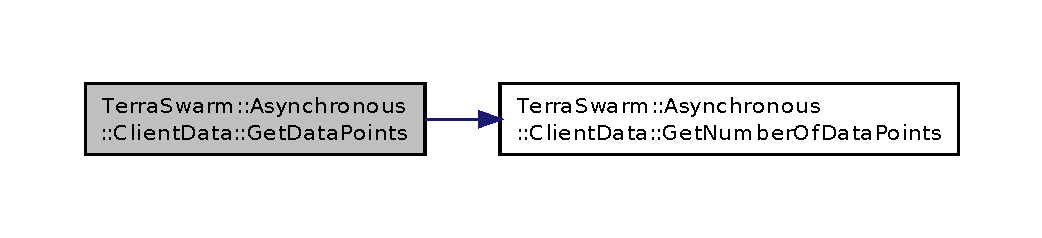
\includegraphics[width=350pt]{class_terra_swarm_1_1_asynchronous_1_1_client_data_a72ed5a08a0bbe088b3b6f4d79cdbab2d_cgraph}
\end{center}
\end{figure}




Here is the caller graph for this function\-:\nopagebreak
\begin{figure}[H]
\begin{center}
\leavevmode
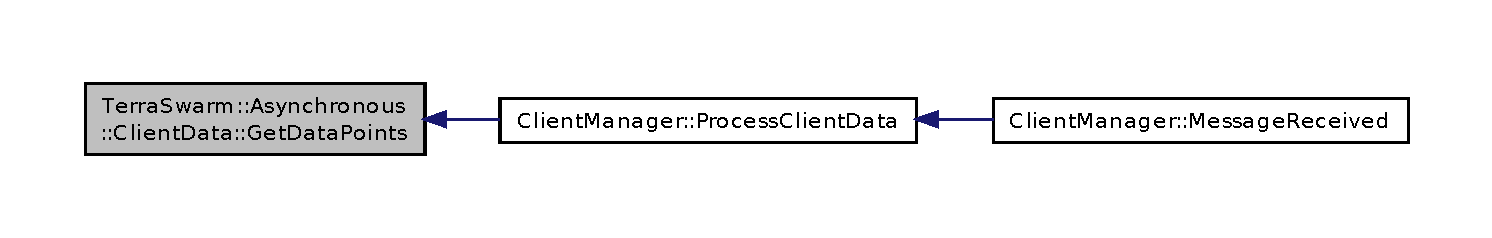
\includegraphics[width=350pt]{class_terra_swarm_1_1_asynchronous_1_1_client_data_a72ed5a08a0bbe088b3b6f4d79cdbab2d_icgraph}
\end{center}
\end{figure}


\hypertarget{class_terra_swarm_1_1_asynchronous_1_1_client_data_abbae8a9d83addb3758fe00fbfeefae97}{\index{Terra\-Swarm\-::\-Asynchronous\-::\-Client\-Data@{Terra\-Swarm\-::\-Asynchronous\-::\-Client\-Data}!Get\-New\-Client\-Data@{Get\-New\-Client\-Data}}
\index{Get\-New\-Client\-Data@{Get\-New\-Client\-Data}!TerraSwarm::Asynchronous::ClientData@{Terra\-Swarm\-::\-Asynchronous\-::\-Client\-Data}}
\subsubsection[{Get\-New\-Client\-Data}]{\setlength{\rightskip}{0pt plus 5cm}{\bf Client\-Data} $\ast$ Terra\-Swarm\-::\-Asynchronous\-::\-Client\-Data\-::\-Get\-New\-Client\-Data (
\begin{DoxyParamCaption}
\item[{const {\bf Message\-Header\-::\-T\-Sender\-Id}}]{sender\-Id, }
\item[{const {\bf Message\-Header\-::\-T\-Receiver\-Id}}]{receiver\-Id, }
\item[{const {\bf T\-Start\-Time}}]{start\-Time, }
\item[{const {\bf T\-Time\-Resolution}}]{time\-Resolution, }
\item[{const {\bf T\-Number\-Of\-Data\-Points}}]{number\-Of\-Data\-Points, }
\item[{{\bf T\-Data\-Point} $\ast$}]{data\-Points}
\end{DoxyParamCaption}
)\hspace{0.3cm}{\ttfamily [static]}}}\label{class_terra_swarm_1_1_asynchronous_1_1_client_data_abbae8a9d83addb3758fe00fbfeefae97}


Creates a new Asnychronous \hyperlink{class_terra_swarm_1_1_asynchronous_1_1_client_data}{Client\-Data} message and allocates memory for it. 

\begin{DoxyWarning}{Warning}
Deallocation is the responsibility of the user.
\end{DoxyWarning}

\begin{DoxyParams}{Parameters}
{\em sender\-Id} & Id of the Sender. \\
\hline
{\em receiver\-Id} & Id of the Receiver. \\
\hline
{\em start\-Time} & Starting time for the first consumption data. \\
\hline
{\em time\-Resolution} & Time interval between consecutive data points. \\
\hline
{\em number\-Of\-Data\-Points} & Number of data points in the message. \\
\hline
{\em data\-Points} & Pointer to the buffer holding the data points.\\
\hline
\end{DoxyParams}
\begin{DoxyReturn}{Returns}
Newly allocated \hyperlink{class_terra_swarm_1_1_asynchronous_1_1_client_data}{Client\-Data} message. 
\end{DoxyReturn}


Definition at line 25 of file Client\-Data.\-cpp.

\hypertarget{class_terra_swarm_1_1_asynchronous_1_1_client_data_aba73075c35dd912dad8f99dd026b0785}{\index{Terra\-Swarm\-::\-Asynchronous\-::\-Client\-Data@{Terra\-Swarm\-::\-Asynchronous\-::\-Client\-Data}!Get\-Number\-Of\-Data\-Points@{Get\-Number\-Of\-Data\-Points}}
\index{Get\-Number\-Of\-Data\-Points@{Get\-Number\-Of\-Data\-Points}!TerraSwarm::Asynchronous::ClientData@{Terra\-Swarm\-::\-Asynchronous\-::\-Client\-Data}}
\subsubsection[{Get\-Number\-Of\-Data\-Points}]{\setlength{\rightskip}{0pt plus 5cm}{\bf Client\-Data\-::\-T\-Number\-Of\-Data\-Points} Terra\-Swarm\-::\-Asynchronous\-::\-Client\-Data\-::\-Get\-Number\-Of\-Data\-Points (
\begin{DoxyParamCaption}
\item[{void}]{}
\end{DoxyParamCaption}
) const}}\label{class_terra_swarm_1_1_asynchronous_1_1_client_data_aba73075c35dd912dad8f99dd026b0785}


Reads the Number\-Of\-Data\-Points field. 

\begin{DoxyReturn}{Returns}
Number of data points in the message. 
\end{DoxyReturn}


Definition at line 76 of file Client\-Data.\-cpp.



Here is the caller graph for this function\-:\nopagebreak
\begin{figure}[H]
\begin{center}
\leavevmode
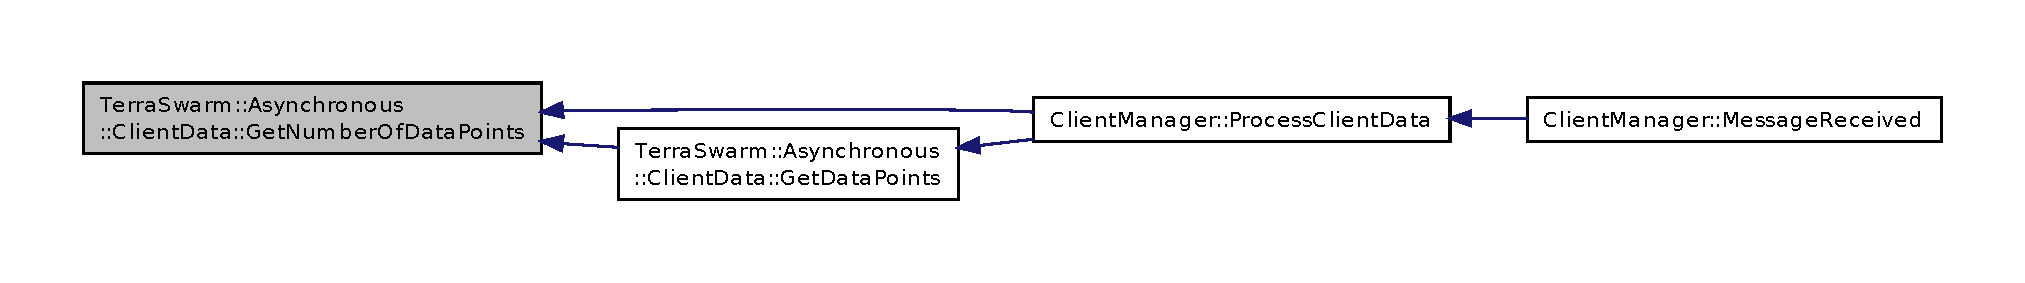
\includegraphics[width=350pt]{class_terra_swarm_1_1_asynchronous_1_1_client_data_aba73075c35dd912dad8f99dd026b0785_icgraph}
\end{center}
\end{figure}


\hypertarget{class_terra_swarm_1_1_asynchronous_1_1_client_data_af78cac737c5197ad17205bab73421b60}{\index{Terra\-Swarm\-::\-Asynchronous\-::\-Client\-Data@{Terra\-Swarm\-::\-Asynchronous\-::\-Client\-Data}!Get\-Start\-Time@{Get\-Start\-Time}}
\index{Get\-Start\-Time@{Get\-Start\-Time}!TerraSwarm::Asynchronous::ClientData@{Terra\-Swarm\-::\-Asynchronous\-::\-Client\-Data}}
\subsubsection[{Get\-Start\-Time}]{\setlength{\rightskip}{0pt plus 5cm}{\bf Client\-Data\-::\-T\-Start\-Time} Terra\-Swarm\-::\-Asynchronous\-::\-Client\-Data\-::\-Get\-Start\-Time (
\begin{DoxyParamCaption}
\item[{void}]{}
\end{DoxyParamCaption}
) const}}\label{class_terra_swarm_1_1_asynchronous_1_1_client_data_af78cac737c5197ad17205bab73421b60}


Reads the Start\-Time field. 

\begin{DoxyReturn}{Returns}
Start\-Time value. 
\end{DoxyReturn}


Definition at line 60 of file Client\-Data.\-cpp.



Here is the caller graph for this function\-:\nopagebreak
\begin{figure}[H]
\begin{center}
\leavevmode
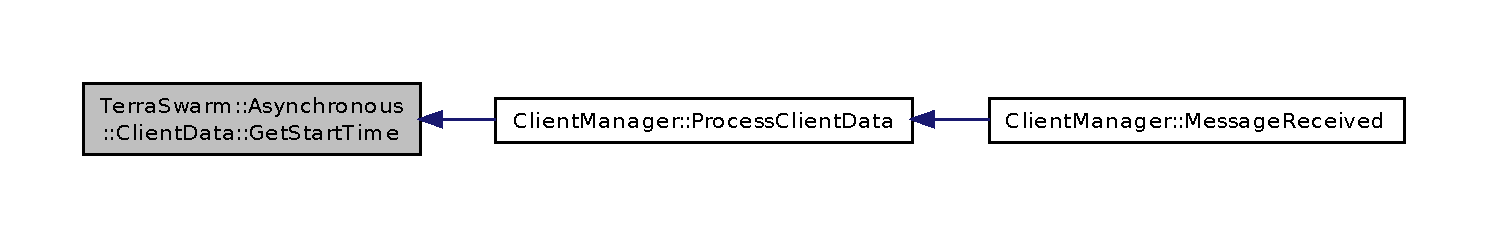
\includegraphics[width=350pt]{class_terra_swarm_1_1_asynchronous_1_1_client_data_af78cac737c5197ad17205bab73421b60_icgraph}
\end{center}
\end{figure}


\hypertarget{class_terra_swarm_1_1_asynchronous_1_1_client_data_a6e3ca8aab58e0b40867eee3e3ec281e6}{\index{Terra\-Swarm\-::\-Asynchronous\-::\-Client\-Data@{Terra\-Swarm\-::\-Asynchronous\-::\-Client\-Data}!Get\-Time\-Resolution@{Get\-Time\-Resolution}}
\index{Get\-Time\-Resolution@{Get\-Time\-Resolution}!TerraSwarm::Asynchronous::ClientData@{Terra\-Swarm\-::\-Asynchronous\-::\-Client\-Data}}
\subsubsection[{Get\-Time\-Resolution}]{\setlength{\rightskip}{0pt plus 5cm}{\bf Client\-Data\-::\-T\-Time\-Resolution} Terra\-Swarm\-::\-Asynchronous\-::\-Client\-Data\-::\-Get\-Time\-Resolution (
\begin{DoxyParamCaption}
\item[{void}]{}
\end{DoxyParamCaption}
) const}}\label{class_terra_swarm_1_1_asynchronous_1_1_client_data_a6e3ca8aab58e0b40867eee3e3ec281e6}


Reads the Time\-Resolution field. 

\begin{DoxyReturn}{Returns}
Time\-Resolution value. 
\end{DoxyReturn}


Definition at line 68 of file Client\-Data.\-cpp.



Here is the caller graph for this function\-:\nopagebreak
\begin{figure}[H]
\begin{center}
\leavevmode
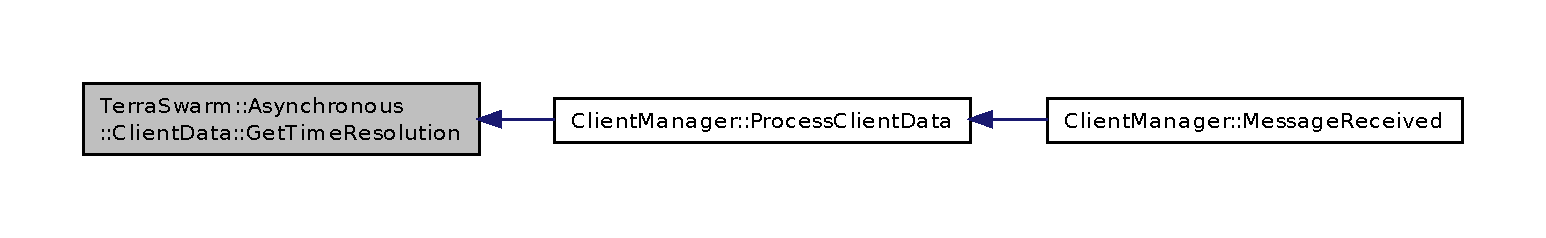
\includegraphics[width=350pt]{class_terra_swarm_1_1_asynchronous_1_1_client_data_a6e3ca8aab58e0b40867eee3e3ec281e6_icgraph}
\end{center}
\end{figure}




The documentation for this class was generated from the following files\-:\begin{DoxyCompactItemize}
\item 
S2\-Sim/\-Terraswarm\-Library/\hyperlink{_client_data_8h}{Client\-Data.\-h}\item 
S2\-Sim/\-Terraswarm\-Library/\hyperlink{_client_data_8cpp}{Client\-Data.\-cpp}\end{DoxyCompactItemize}

\hypertarget{class_terra_swarm_1_1_synchronous_1_1_client_data}{\section{Terra\-Swarm\-:\-:Synchronous\-:\-:Client\-Data Class Reference}
\label{class_terra_swarm_1_1_synchronous_1_1_client_data}\index{Terra\-Swarm\-::\-Synchronous\-::\-Client\-Data@{Terra\-Swarm\-::\-Synchronous\-::\-Client\-Data}}
}


\hyperlink{namespace_terra_swarm_1_1_synchronous}{Synchronous} Client Data message from the client to indicate its consumption for a time interval.  




{\ttfamily \#include $<$Client\-Data.\-h$>$}

\subsection*{Public Types}
\begin{DoxyCompactItemize}
\item 
enum \hyperlink{class_terra_swarm_1_1_synchronous_1_1_client_data_ab069b9069716e25b2e5be34d2356ec01}{Check\-Result\-Values} \{ \hyperlink{class_terra_swarm_1_1_synchronous_1_1_client_data_ab069b9069716e25b2e5be34d2356ec01a655e724c0fe6463a22105e8c629a345d}{Success} = ( T\-Check\-Result )true, 
\hyperlink{class_terra_swarm_1_1_synchronous_1_1_client_data_ab069b9069716e25b2e5be34d2356ec01a12ebd40706bb9823852ae1688e87e831}{Fail} = ( T\-Check\-Result )false
 \}
\begin{DoxyCompactList}\small\item\em Defines the values for T\-Check\-Result. \end{DoxyCompactList}\item 
typedef bool \hyperlink{class_terra_swarm_1_1_synchronous_1_1_client_data_a2a4af9153f7e8fe6cadba6a188ce2207}{T\-Check\-Result}
\begin{DoxyCompactList}\small\item\em Defines the message check result type. \end{DoxyCompactList}\item 
typedef unsigned int \hyperlink{class_terra_swarm_1_1_synchronous_1_1_client_data_a6c581f1f80217390ea8fe95136c60f07}{T\-Data\-Point}
\begin{DoxyCompactList}\small\item\em Defines the type for a general data point, consumption in this case. \end{DoxyCompactList}\end{DoxyCompactItemize}
\subsection*{Public Member Functions}
\begin{DoxyCompactItemize}
\item 
\hyperlink{class_terra_swarm_1_1_synchronous_1_1_client_data_a67bc913ce1ebd9641da07bdc09e4444e}{$\sim$\-Client\-Data} (void)
\begin{DoxyCompactList}\small\item\em Deallocates the memory. \end{DoxyCompactList}\item 
\hyperlink{class_terra_swarm_1_1_synchronous_1_1_client_data_a2a4af9153f7e8fe6cadba6a188ce2207}{T\-Check\-Result} \hyperlink{class_terra_swarm_1_1_synchronous_1_1_client_data_a49c4a96e9b957c237f40aad39e7cb328}{Check\-Message} (void) const 
\begin{DoxyCompactList}\small\item\em Checks whether the current memory contains a \hyperlink{class_terra_swarm_1_1_synchronous_1_1_client_data}{Client\-Data} message. \end{DoxyCompactList}\item 
\hyperlink{class_terra_swarm_1_1_synchronous_1_1_client_data_a6c581f1f80217390ea8fe95136c60f07}{T\-Data\-Point} \hyperlink{class_terra_swarm_1_1_synchronous_1_1_client_data_ac71da8ed6f56cfdac3f01131f6bef342}{Get\-Data\-Point} (void) const 
\begin{DoxyCompactList}\small\item\em Reads the data point in the message. \end{DoxyCompactList}\end{DoxyCompactItemize}
\subsection*{Static Public Member Functions}
\begin{DoxyCompactItemize}
\item 
static \hyperlink{class_terra_swarm_1_1_synchronous_1_1_client_data}{Client\-Data} $\ast$ \hyperlink{class_terra_swarm_1_1_synchronous_1_1_client_data_a5b055348cbcd27e656744b51d98c1ab2}{Get\-New\-Client\-Data} (const \hyperlink{class_terra_swarm_1_1_message_header_a516b36855e2aad7cfbf8770f1b42784f}{Message\-Header\-::\-T\-Sender\-Id} sender\-Id, const \hyperlink{class_terra_swarm_1_1_message_header_aa3260702b182b6f88ddbdd3416e98df0}{Message\-Header\-::\-T\-Receiver\-Id} receiver\-Id, \hyperlink{class_terra_swarm_1_1_synchronous_1_1_client_data_a6c581f1f80217390ea8fe95136c60f07}{T\-Data\-Point} data\-Point)
\begin{DoxyCompactList}\small\item\em Constructs a new \hyperlink{class_terra_swarm_1_1_synchronous_1_1_client_data}{Client\-Data} message and allocates the necessary memory for it. \end{DoxyCompactList}\end{DoxyCompactItemize}
\subsection*{Private Types}
\begin{DoxyCompactItemize}
\item 
enum \hyperlink{class_terra_swarm_1_1_synchronous_1_1_client_data_a529711f4bde913bbc871ba784b668cb5}{Header\-Values} \{ \hyperlink{class_terra_swarm_1_1_synchronous_1_1_client_data_a529711f4bde913bbc871ba784b668cb5acfabe23548b5afe59eb4880618ebd082}{Message\-Type} = 0x0003, 
\hyperlink{class_terra_swarm_1_1_synchronous_1_1_client_data_a529711f4bde913bbc871ba784b668cb5a2025f950fc35f0a838bc4b72d5fd5e8c}{Message\-Id} = 0x0005
 \}
\begin{DoxyCompactList}\small\item\em Message Header Values. \end{DoxyCompactList}\item 
enum \hyperlink{class_terra_swarm_1_1_synchronous_1_1_client_data_aae90a1a7ba3ea4c66542d1c3c9f2e6d9}{Field\-Size\-Values} \{ \hyperlink{class_terra_swarm_1_1_synchronous_1_1_client_data_aae90a1a7ba3ea4c66542d1c3c9f2e6d9aca053edd8f58cbd2cb277d7cfad9a419}{Data\-Point\-Size} = sizeof( T\-Data\-Point )
 \}
\begin{DoxyCompactList}\small\item\em Size of the fields within the message. \end{DoxyCompactList}\item 
enum \hyperlink{class_terra_swarm_1_1_synchronous_1_1_client_data_a46332e5dcabec8b7327933a990299886}{Field\-Index\-Values} \{ \hyperlink{class_terra_swarm_1_1_synchronous_1_1_client_data_a46332e5dcabec8b7327933a990299886a459dcd5d2d9c725f12d2b5a8175f40b7}{Data\-Start\-Index} = Message\-Header\-:\-:Message\-Header\-Size
 \}
\begin{DoxyCompactList}\small\item\em Index of the fields within the message. \end{DoxyCompactList}\item 
typedef \hyperlink{class_terra_swarm_1_1_network_byte_accessor}{Network\-Byte\-Accessor}\\*
$<$ \hyperlink{class_terra_swarm_1_1_synchronous_1_1_client_data_a46332e5dcabec8b7327933a990299886a459dcd5d2d9c725f12d2b5a8175f40b7}{Data\-Start\-Index}, \\*
\hyperlink{class_terra_swarm_1_1_synchronous_1_1_client_data_aae90a1a7ba3ea4c66542d1c3c9f2e6d9aca053edd8f58cbd2cb277d7cfad9a419}{Data\-Point\-Size} $>$ \hyperlink{class_terra_swarm_1_1_synchronous_1_1_client_data_a69ba4da130856d78eec92c6dcdb61c58}{T\-Data\-Point\-Accessor}
\begin{DoxyCompactList}\small\item\em Accessor helper for the Data\-Point field. \end{DoxyCompactList}\end{DoxyCompactItemize}
\subsection*{Private Member Functions}
\begin{DoxyCompactItemize}
\item 
\hyperlink{class_terra_swarm_1_1_synchronous_1_1_client_data_a55b91e768e21a3e176ed03b504182ca3}{Client\-Data} (void)
\begin{DoxyCompactList}\small\item\em Private constructor to force the usage of the static construction method. \end{DoxyCompactList}\end{DoxyCompactItemize}


\subsection{Detailed Description}
\hyperlink{namespace_terra_swarm_1_1_synchronous}{Synchronous} Client Data message from the client to indicate its consumption for a time interval. 

Definition at line 188 of file Client\-Data.\-h.



\subsection{Member Typedef Documentation}
\hypertarget{class_terra_swarm_1_1_synchronous_1_1_client_data_a2a4af9153f7e8fe6cadba6a188ce2207}{\index{Terra\-Swarm\-::\-Synchronous\-::\-Client\-Data@{Terra\-Swarm\-::\-Synchronous\-::\-Client\-Data}!T\-Check\-Result@{T\-Check\-Result}}
\index{T\-Check\-Result@{T\-Check\-Result}!TerraSwarm::Synchronous::ClientData@{Terra\-Swarm\-::\-Synchronous\-::\-Client\-Data}}
\subsubsection[{T\-Check\-Result}]{\setlength{\rightskip}{0pt plus 5cm}typedef bool {\bf Terra\-Swarm\-::\-Synchronous\-::\-Client\-Data\-::\-T\-Check\-Result}}}\label{class_terra_swarm_1_1_synchronous_1_1_client_data_a2a4af9153f7e8fe6cadba6a188ce2207}


Defines the message check result type. 



Definition at line 204 of file Client\-Data.\-h.

\hypertarget{class_terra_swarm_1_1_synchronous_1_1_client_data_a6c581f1f80217390ea8fe95136c60f07}{\index{Terra\-Swarm\-::\-Synchronous\-::\-Client\-Data@{Terra\-Swarm\-::\-Synchronous\-::\-Client\-Data}!T\-Data\-Point@{T\-Data\-Point}}
\index{T\-Data\-Point@{T\-Data\-Point}!TerraSwarm::Synchronous::ClientData@{Terra\-Swarm\-::\-Synchronous\-::\-Client\-Data}}
\subsubsection[{T\-Data\-Point}]{\setlength{\rightskip}{0pt plus 5cm}typedef unsigned int {\bf Terra\-Swarm\-::\-Synchronous\-::\-Client\-Data\-::\-T\-Data\-Point}}}\label{class_terra_swarm_1_1_synchronous_1_1_client_data_a6c581f1f80217390ea8fe95136c60f07}


Defines the type for a general data point, consumption in this case. 



Definition at line 218 of file Client\-Data.\-h.

\hypertarget{class_terra_swarm_1_1_synchronous_1_1_client_data_a69ba4da130856d78eec92c6dcdb61c58}{\index{Terra\-Swarm\-::\-Synchronous\-::\-Client\-Data@{Terra\-Swarm\-::\-Synchronous\-::\-Client\-Data}!T\-Data\-Point\-Accessor@{T\-Data\-Point\-Accessor}}
\index{T\-Data\-Point\-Accessor@{T\-Data\-Point\-Accessor}!TerraSwarm::Synchronous::ClientData@{Terra\-Swarm\-::\-Synchronous\-::\-Client\-Data}}
\subsubsection[{T\-Data\-Point\-Accessor}]{\setlength{\rightskip}{0pt plus 5cm}typedef {\bf Network\-Byte\-Accessor}$<${\bf Data\-Start\-Index}, {\bf Data\-Point\-Size}$>$ {\bf Terra\-Swarm\-::\-Synchronous\-::\-Client\-Data\-::\-T\-Data\-Point\-Accessor}\hspace{0.3cm}{\ttfamily [private]}}}\label{class_terra_swarm_1_1_synchronous_1_1_client_data_a69ba4da130856d78eec92c6dcdb61c58}


Accessor helper for the Data\-Point field. 



Definition at line 240 of file Client\-Data.\-h.



\subsection{Member Enumeration Documentation}
\hypertarget{class_terra_swarm_1_1_synchronous_1_1_client_data_ab069b9069716e25b2e5be34d2356ec01}{\index{Terra\-Swarm\-::\-Synchronous\-::\-Client\-Data@{Terra\-Swarm\-::\-Synchronous\-::\-Client\-Data}!Check\-Result\-Values@{Check\-Result\-Values}}
\index{Check\-Result\-Values@{Check\-Result\-Values}!TerraSwarm::Synchronous::ClientData@{Terra\-Swarm\-::\-Synchronous\-::\-Client\-Data}}
\subsubsection[{Check\-Result\-Values}]{\setlength{\rightskip}{0pt plus 5cm}enum {\bf Terra\-Swarm\-::\-Synchronous\-::\-Client\-Data\-::\-Check\-Result\-Values}}}\label{class_terra_swarm_1_1_synchronous_1_1_client_data_ab069b9069716e25b2e5be34d2356ec01}


Defines the values for T\-Check\-Result. 

\begin{Desc}
\item[Enumerator]\par
\begin{description}
\index{Success@{Success}!Terra\-Swarm\-::\-Synchronous\-::\-Client\-Data@{Terra\-Swarm\-::\-Synchronous\-::\-Client\-Data}}\index{Terra\-Swarm\-::\-Synchronous\-::\-Client\-Data@{Terra\-Swarm\-::\-Synchronous\-::\-Client\-Data}!Success@{Success}}\item[{\em 
\hypertarget{class_terra_swarm_1_1_synchronous_1_1_client_data_ab069b9069716e25b2e5be34d2356ec01a655e724c0fe6463a22105e8c629a345d}{Success}\label{class_terra_swarm_1_1_synchronous_1_1_client_data_ab069b9069716e25b2e5be34d2356ec01a655e724c0fe6463a22105e8c629a345d}
}]Message is of correct type and id. \index{Fail@{Fail}!Terra\-Swarm\-::\-Synchronous\-::\-Client\-Data@{Terra\-Swarm\-::\-Synchronous\-::\-Client\-Data}}\index{Terra\-Swarm\-::\-Synchronous\-::\-Client\-Data@{Terra\-Swarm\-::\-Synchronous\-::\-Client\-Data}!Fail@{Fail}}\item[{\em 
\hypertarget{class_terra_swarm_1_1_synchronous_1_1_client_data_ab069b9069716e25b2e5be34d2356ec01a12ebd40706bb9823852ae1688e87e831}{Fail}\label{class_terra_swarm_1_1_synchronous_1_1_client_data_ab069b9069716e25b2e5be34d2356ec01a12ebd40706bb9823852ae1688e87e831}
}]Message has incorrect type or id. \end{description}
\end{Desc}


Definition at line 209 of file Client\-Data.\-h.

\hypertarget{class_terra_swarm_1_1_synchronous_1_1_client_data_a46332e5dcabec8b7327933a990299886}{\index{Terra\-Swarm\-::\-Synchronous\-::\-Client\-Data@{Terra\-Swarm\-::\-Synchronous\-::\-Client\-Data}!Field\-Index\-Values@{Field\-Index\-Values}}
\index{Field\-Index\-Values@{Field\-Index\-Values}!TerraSwarm::Synchronous::ClientData@{Terra\-Swarm\-::\-Synchronous\-::\-Client\-Data}}
\subsubsection[{Field\-Index\-Values}]{\setlength{\rightskip}{0pt plus 5cm}enum {\bf Terra\-Swarm\-::\-Synchronous\-::\-Client\-Data\-::\-Field\-Index\-Values}\hspace{0.3cm}{\ttfamily [private]}}}\label{class_terra_swarm_1_1_synchronous_1_1_client_data_a46332e5dcabec8b7327933a990299886}


Index of the fields within the message. 

\begin{Desc}
\item[Enumerator]\par
\begin{description}
\index{Data\-Start\-Index@{Data\-Start\-Index}!Terra\-Swarm\-::\-Synchronous\-::\-Client\-Data@{Terra\-Swarm\-::\-Synchronous\-::\-Client\-Data}}\index{Terra\-Swarm\-::\-Synchronous\-::\-Client\-Data@{Terra\-Swarm\-::\-Synchronous\-::\-Client\-Data}!Data\-Start\-Index@{Data\-Start\-Index}}\item[{\em 
\hypertarget{class_terra_swarm_1_1_synchronous_1_1_client_data_a46332e5dcabec8b7327933a990299886a459dcd5d2d9c725f12d2b5a8175f40b7}{Data\-Start\-Index}\label{class_terra_swarm_1_1_synchronous_1_1_client_data_a46332e5dcabec8b7327933a990299886a459dcd5d2d9c725f12d2b5a8175f40b7}
}]\end{description}
\end{Desc}


Definition at line 232 of file Client\-Data.\-h.

\hypertarget{class_terra_swarm_1_1_synchronous_1_1_client_data_aae90a1a7ba3ea4c66542d1c3c9f2e6d9}{\index{Terra\-Swarm\-::\-Synchronous\-::\-Client\-Data@{Terra\-Swarm\-::\-Synchronous\-::\-Client\-Data}!Field\-Size\-Values@{Field\-Size\-Values}}
\index{Field\-Size\-Values@{Field\-Size\-Values}!TerraSwarm::Synchronous::ClientData@{Terra\-Swarm\-::\-Synchronous\-::\-Client\-Data}}
\subsubsection[{Field\-Size\-Values}]{\setlength{\rightskip}{0pt plus 5cm}enum {\bf Terra\-Swarm\-::\-Synchronous\-::\-Client\-Data\-::\-Field\-Size\-Values}\hspace{0.3cm}{\ttfamily [private]}}}\label{class_terra_swarm_1_1_synchronous_1_1_client_data_aae90a1a7ba3ea4c66542d1c3c9f2e6d9}


Size of the fields within the message. 

\begin{Desc}
\item[Enumerator]\par
\begin{description}
\index{Data\-Point\-Size@{Data\-Point\-Size}!Terra\-Swarm\-::\-Synchronous\-::\-Client\-Data@{Terra\-Swarm\-::\-Synchronous\-::\-Client\-Data}}\index{Terra\-Swarm\-::\-Synchronous\-::\-Client\-Data@{Terra\-Swarm\-::\-Synchronous\-::\-Client\-Data}!Data\-Point\-Size@{Data\-Point\-Size}}\item[{\em 
\hypertarget{class_terra_swarm_1_1_synchronous_1_1_client_data_aae90a1a7ba3ea4c66542d1c3c9f2e6d9aca053edd8f58cbd2cb277d7cfad9a419}{Data\-Point\-Size}\label{class_terra_swarm_1_1_synchronous_1_1_client_data_aae90a1a7ba3ea4c66542d1c3c9f2e6d9aca053edd8f58cbd2cb277d7cfad9a419}
}]\end{description}
\end{Desc}


Definition at line 224 of file Client\-Data.\-h.

\hypertarget{class_terra_swarm_1_1_synchronous_1_1_client_data_a529711f4bde913bbc871ba784b668cb5}{\index{Terra\-Swarm\-::\-Synchronous\-::\-Client\-Data@{Terra\-Swarm\-::\-Synchronous\-::\-Client\-Data}!Header\-Values@{Header\-Values}}
\index{Header\-Values@{Header\-Values}!TerraSwarm::Synchronous::ClientData@{Terra\-Swarm\-::\-Synchronous\-::\-Client\-Data}}
\subsubsection[{Header\-Values}]{\setlength{\rightskip}{0pt plus 5cm}enum {\bf Terra\-Swarm\-::\-Synchronous\-::\-Client\-Data\-::\-Header\-Values}\hspace{0.3cm}{\ttfamily [private]}}}\label{class_terra_swarm_1_1_synchronous_1_1_client_data_a529711f4bde913bbc871ba784b668cb5}


Message Header Values. 

\begin{Desc}
\item[Enumerator]\par
\begin{description}
\index{Message\-Type@{Message\-Type}!Terra\-Swarm\-::\-Synchronous\-::\-Client\-Data@{Terra\-Swarm\-::\-Synchronous\-::\-Client\-Data}}\index{Terra\-Swarm\-::\-Synchronous\-::\-Client\-Data@{Terra\-Swarm\-::\-Synchronous\-::\-Client\-Data}!Message\-Type@{Message\-Type}}\item[{\em 
\hypertarget{class_terra_swarm_1_1_synchronous_1_1_client_data_a529711f4bde913bbc871ba784b668cb5acfabe23548b5afe59eb4880618ebd082}{Message\-Type}\label{class_terra_swarm_1_1_synchronous_1_1_client_data_a529711f4bde913bbc871ba784b668cb5acfabe23548b5afe59eb4880618ebd082}
}]\index{Message\-Id@{Message\-Id}!Terra\-Swarm\-::\-Synchronous\-::\-Client\-Data@{Terra\-Swarm\-::\-Synchronous\-::\-Client\-Data}}\index{Terra\-Swarm\-::\-Synchronous\-::\-Client\-Data@{Terra\-Swarm\-::\-Synchronous\-::\-Client\-Data}!Message\-Id@{Message\-Id}}\item[{\em 
\hypertarget{class_terra_swarm_1_1_synchronous_1_1_client_data_a529711f4bde913bbc871ba784b668cb5a2025f950fc35f0a838bc4b72d5fd5e8c}{Message\-Id}\label{class_terra_swarm_1_1_synchronous_1_1_client_data_a529711f4bde913bbc871ba784b668cb5a2025f950fc35f0a838bc4b72d5fd5e8c}
}]\end{description}
\end{Desc}


Definition at line 194 of file Client\-Data.\-h.



\subsection{Constructor \& Destructor Documentation}
\hypertarget{class_terra_swarm_1_1_synchronous_1_1_client_data_a55b91e768e21a3e176ed03b504182ca3}{\index{Terra\-Swarm\-::\-Synchronous\-::\-Client\-Data@{Terra\-Swarm\-::\-Synchronous\-::\-Client\-Data}!Client\-Data@{Client\-Data}}
\index{Client\-Data@{Client\-Data}!TerraSwarm::Synchronous::ClientData@{Terra\-Swarm\-::\-Synchronous\-::\-Client\-Data}}
\subsubsection[{Client\-Data}]{\setlength{\rightskip}{0pt plus 5cm}Terra\-Swarm\-::\-Synchronous\-::\-Client\-Data\-::\-Client\-Data (
\begin{DoxyParamCaption}
\item[{void}]{}
\end{DoxyParamCaption}
)\hspace{0.3cm}{\ttfamily [private]}}}\label{class_terra_swarm_1_1_synchronous_1_1_client_data_a55b91e768e21a3e176ed03b504182ca3}


Private constructor to force the usage of the static construction method. 



Definition at line 97 of file Client\-Data.\-cpp.

\hypertarget{class_terra_swarm_1_1_synchronous_1_1_client_data_a67bc913ce1ebd9641da07bdc09e4444e}{\index{Terra\-Swarm\-::\-Synchronous\-::\-Client\-Data@{Terra\-Swarm\-::\-Synchronous\-::\-Client\-Data}!$\sim$\-Client\-Data@{$\sim$\-Client\-Data}}
\index{$\sim$\-Client\-Data@{$\sim$\-Client\-Data}!TerraSwarm::Synchronous::ClientData@{Terra\-Swarm\-::\-Synchronous\-::\-Client\-Data}}
\subsubsection[{$\sim$\-Client\-Data}]{\setlength{\rightskip}{0pt plus 5cm}Terra\-Swarm\-::\-Synchronous\-::\-Client\-Data\-::$\sim$\-Client\-Data (
\begin{DoxyParamCaption}
\item[{void}]{}
\end{DoxyParamCaption}
)}}\label{class_terra_swarm_1_1_synchronous_1_1_client_data_a67bc913ce1ebd9641da07bdc09e4444e}


Deallocates the memory. 



Definition at line 101 of file Client\-Data.\-cpp.



\subsection{Member Function Documentation}
\hypertarget{class_terra_swarm_1_1_synchronous_1_1_client_data_a49c4a96e9b957c237f40aad39e7cb328}{\index{Terra\-Swarm\-::\-Synchronous\-::\-Client\-Data@{Terra\-Swarm\-::\-Synchronous\-::\-Client\-Data}!Check\-Message@{Check\-Message}}
\index{Check\-Message@{Check\-Message}!TerraSwarm::Synchronous::ClientData@{Terra\-Swarm\-::\-Synchronous\-::\-Client\-Data}}
\subsubsection[{Check\-Message}]{\setlength{\rightskip}{0pt plus 5cm}{\bf Client\-Data\-::\-T\-Check\-Result} Terra\-Swarm\-::\-Synchronous\-::\-Client\-Data\-::\-Check\-Message (
\begin{DoxyParamCaption}
\item[{void}]{}
\end{DoxyParamCaption}
) const}}\label{class_terra_swarm_1_1_synchronous_1_1_client_data_a49c4a96e9b957c237f40aad39e7cb328}


Checks whether the current memory contains a \hyperlink{class_terra_swarm_1_1_synchronous_1_1_client_data}{Client\-Data} message. 

\begin{DoxyReturn}{Returns}
Result of the check. 
\end{DoxyReturn}


Definition at line 122 of file Client\-Data.\-cpp.

\hypertarget{class_terra_swarm_1_1_synchronous_1_1_client_data_ac71da8ed6f56cfdac3f01131f6bef342}{\index{Terra\-Swarm\-::\-Synchronous\-::\-Client\-Data@{Terra\-Swarm\-::\-Synchronous\-::\-Client\-Data}!Get\-Data\-Point@{Get\-Data\-Point}}
\index{Get\-Data\-Point@{Get\-Data\-Point}!TerraSwarm::Synchronous::ClientData@{Terra\-Swarm\-::\-Synchronous\-::\-Client\-Data}}
\subsubsection[{Get\-Data\-Point}]{\setlength{\rightskip}{0pt plus 5cm}{\bf Client\-Data\-::\-T\-Data\-Point} Terra\-Swarm\-::\-Synchronous\-::\-Client\-Data\-::\-Get\-Data\-Point (
\begin{DoxyParamCaption}
\item[{void}]{}
\end{DoxyParamCaption}
) const}}\label{class_terra_swarm_1_1_synchronous_1_1_client_data_ac71da8ed6f56cfdac3f01131f6bef342}


Reads the data point in the message. 

\begin{DoxyReturn}{Returns}
Data point value. 
\end{DoxyReturn}


Definition at line 133 of file Client\-Data.\-cpp.



Here is the caller graph for this function\-:\nopagebreak
\begin{figure}[H]
\begin{center}
\leavevmode
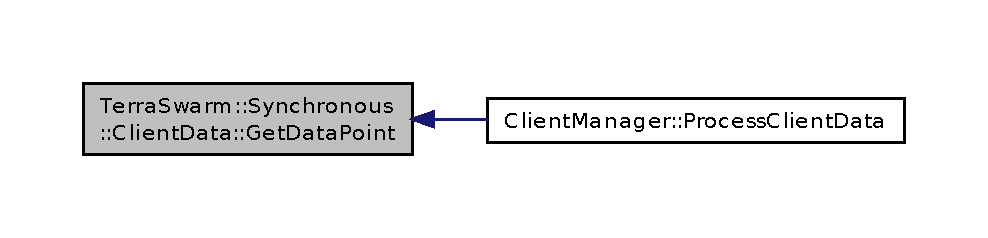
\includegraphics[width=350pt]{class_terra_swarm_1_1_synchronous_1_1_client_data_ac71da8ed6f56cfdac3f01131f6bef342_icgraph}
\end{center}
\end{figure}


\hypertarget{class_terra_swarm_1_1_synchronous_1_1_client_data_a5b055348cbcd27e656744b51d98c1ab2}{\index{Terra\-Swarm\-::\-Synchronous\-::\-Client\-Data@{Terra\-Swarm\-::\-Synchronous\-::\-Client\-Data}!Get\-New\-Client\-Data@{Get\-New\-Client\-Data}}
\index{Get\-New\-Client\-Data@{Get\-New\-Client\-Data}!TerraSwarm::Synchronous::ClientData@{Terra\-Swarm\-::\-Synchronous\-::\-Client\-Data}}
\subsubsection[{Get\-New\-Client\-Data}]{\setlength{\rightskip}{0pt plus 5cm}{\bf Client\-Data} $\ast$ Terra\-Swarm\-::\-Synchronous\-::\-Client\-Data\-::\-Get\-New\-Client\-Data (
\begin{DoxyParamCaption}
\item[{const {\bf Message\-Header\-::\-T\-Sender\-Id}}]{sender\-Id, }
\item[{const {\bf Message\-Header\-::\-T\-Receiver\-Id}}]{receiver\-Id, }
\item[{{\bf T\-Data\-Point}}]{data\-Point}
\end{DoxyParamCaption}
)\hspace{0.3cm}{\ttfamily [static]}}}\label{class_terra_swarm_1_1_synchronous_1_1_client_data_a5b055348cbcd27e656744b51d98c1ab2}


Constructs a new \hyperlink{class_terra_swarm_1_1_synchronous_1_1_client_data}{Client\-Data} message and allocates the necessary memory for it. 

\begin{DoxyWarning}{Warning}
Deallocation is the responsibility of the user.
\end{DoxyWarning}

\begin{DoxyParams}{Parameters}
{\em sender\-Id} & Id of the sender. \\
\hline
{\em receiver\-Id} & Id of the receiver. \\
\hline
{\em data\-Point} & Consumption of the user for the next time interval.\\
\hline
\end{DoxyParams}
\begin{DoxyReturn}{Returns}
Newly allocated \hyperlink{class_terra_swarm_1_1_synchronous_1_1_client_data}{Client\-Data} message. 
\end{DoxyReturn}


Definition at line 107 of file Client\-Data.\-cpp.



The documentation for this class was generated from the following files\-:\begin{DoxyCompactItemize}
\item 
S2\-Sim/\-Terraswarm\-Library/\hyperlink{_client_data_8h}{Client\-Data.\-h}\item 
S2\-Sim/\-Terraswarm\-Library/\hyperlink{_client_data_8cpp}{Client\-Data.\-cpp}\end{DoxyCompactItemize}

\hypertarget{class_client_manager}{\section{Client\-Manager Class Reference}
\label{class_client_manager}\index{Client\-Manager@{Client\-Manager}}
}


Manages the connection with a client.  




{\ttfamily \#include $<$Client\-Manager.\-h$>$}



Collaboration diagram for Client\-Manager\-:\nopagebreak
\begin{figure}[H]
\begin{center}
\leavevmode
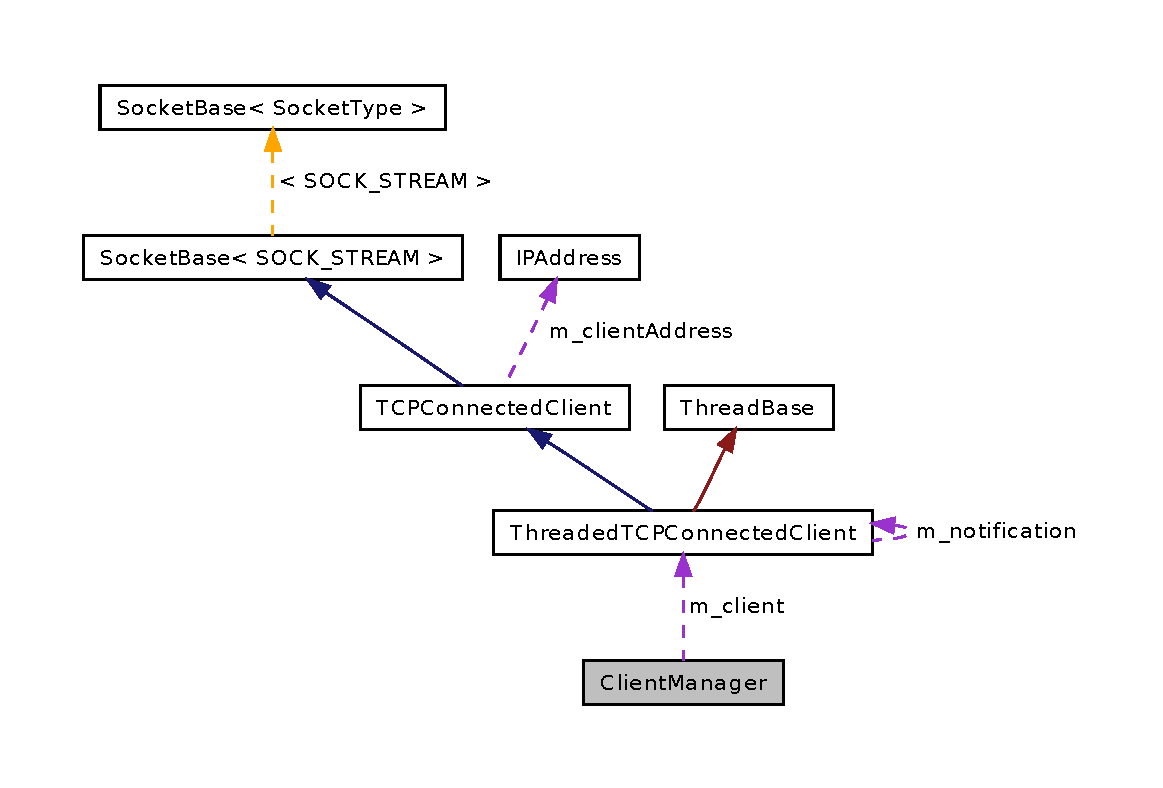
\includegraphics[width=350pt]{class_client_manager__coll__graph}
\end{center}
\end{figure}
\subsection*{Public Types}
\begin{DoxyCompactItemize}
\item 
typedef \\*
\hyperlink{class_terra_swarm_1_1_synchronous_1_1_set_current_price_a2ed14f2a90070d19a70183bb63e7708e}{Synchronous\-::\-Set\-Current\-Price\-::\-T\-Price} \hyperlink{class_client_manager_ae957a71b432eb6d9d39b0f397cd89874}{T\-Price}
\item 
typedef \\*
\hyperlink{class_terra_swarm_1_1_synchronous_1_1_set_current_price_aa87902078a0788d13ef70b899d83f4d3}{Synchronous\-::\-Set\-Current\-Price\-::\-T\-Interval} \hyperlink{class_client_manager_a429cc3229a8121c83655945ebaec18a6}{T\-Interval}
\end{DoxyCompactItemize}
\subsection*{Public Member Functions}
\begin{DoxyCompactItemize}
\item 
\hyperlink{class_client_manager_ad012b20c788f625e98e09e849744a8d9}{Client\-Manager} (void)
\begin{DoxyCompactList}\small\item\em Default constructor. \end{DoxyCompactList}\item 
\hyperlink{class_client_manager_acdcd9f65fd1f9c819e9d8a8130e661ca}{Client\-Manager} (\hyperlink{class_threaded_t_c_p_connected_client}{Threaded\-T\-C\-P\-Connected\-Client} $\ast$client)
\begin{DoxyCompactList}\small\item\em Constructs the client manager with a connection. \end{DoxyCompactList}\item 
\hyperlink{class_client_manager_aa99b4fc6e351914f367db37ea83d1e65}{Client\-Manager} (const \hyperlink{class_client_manager}{Client\-Manager} \&copy)
\begin{DoxyCompactList}\small\item\em Copy constructor. \end{DoxyCompactList}\item 
\hyperlink{class_client_manager_abac29dfed67c8b8354cf07267fd5515b}{$\sim$\-Client\-Manager} (void)
\begin{DoxyCompactList}\small\item\em Destructor, deletes the connection. \end{DoxyCompactList}\item 
\hyperlink{class_client_manager}{Client\-Manager} \& \hyperlink{class_client_manager_a1b3ae7dda1e6d1a2939c3eb6a1b9cbd1}{operator=} (const \hyperlink{class_client_manager}{Client\-Manager} \&copy)
\begin{DoxyCompactList}\small\item\em Copies the contents of another client manager. \end{DoxyCompactList}\item 
void \hyperlink{class_client_manager_a4fa8fc5731587276f5e6be92563474fa}{Connection\-Broken} (void)
\begin{DoxyCompactList}\small\item\em Handles the broken connection case. \end{DoxyCompactList}\item 
void \hyperlink{class_client_manager_abf05d2ac88337dfd02e0b7986ee1e18c}{Message\-Received} (void $\ast$data, const size\-\_\-t data\-Size)
\begin{DoxyCompactList}\small\item\em Called when a message is received. \end{DoxyCompactList}\item 
void \hyperlink{class_client_manager_adb64a2ee5d0eb7b1a4bdedcd0e3b92f5}{Set\-Current\-Price} (const \hyperlink{class_client_manager_ae957a71b432eb6d9d39b0f397cd89874}{T\-Price} price, const \hyperlink{class_client_manager_a429cc3229a8121c83655945ebaec18a6}{T\-Interval} begin\-Interval, const \hyperlink{class_client_manager_a429cc3229a8121c83655945ebaec18a6}{T\-Interval} end\-Interval)
\item 
void \hyperlink{class_client_manager_ae297765312b5f2f93f7b8ec700ad2fbb}{Price\-Proposal} (const \hyperlink{class_client_manager_ae957a71b432eb6d9d39b0f397cd89874}{T\-Price} price, const \hyperlink{class_client_manager_a429cc3229a8121c83655945ebaec18a6}{T\-Interval} begin\-Interval, const \hyperlink{class_client_manager_a429cc3229a8121c83655945ebaec18a6}{T\-Interval} end\-Interval)
\item 
bool \hyperlink{class_client_manager_a626b9383b2b2b7924a1f1e183800fe72}{Is\-Synchronous} (void) const 
\item 
bool \hyperlink{class_client_manager_ab3f0c2bb301ba8d1218d703e5446baf3}{Is\-Asynchronous} (void) const 
\end{DoxyCompactItemize}
\subsection*{Private Types}
\begin{DoxyCompactItemize}
\item 
enum \hyperlink{class_client_manager_ac12239be9a30847f677a32910822d40b}{Client\-Type\-Values} \{ \hyperlink{class_client_manager_ac12239be9a30847f677a32910822d40ba5efa5897435cfd442d637beea251c85a}{Asynchronous\-Client} = ( T\-Client\-Type )0x01, 
\hyperlink{class_client_manager_ac12239be9a30847f677a32910822d40bada4fe5ba56979f1deaf93b69d0a8fcae}{Synchronous\-Client} = ( T\-Client\-Type )0x02
 \}
\item 
typedef unsigned char \hyperlink{class_client_manager_a223aecacabe855f08e4675b12403dfa4}{T\-Client\-Type}
\item 
typedef \hyperlink{class_terra_swarm_1_1_message_header_ab55de822fadad758edcd8f36bd07676e}{Message\-Header\-::\-T\-Id} \hyperlink{class_client_manager_a531e5e7eb779e8ce3c47b8eabd8e9b17}{T\-Id}
\end{DoxyCompactItemize}
\subsection*{Private Member Functions}
\begin{DoxyCompactItemize}
\item 
void \hyperlink{class_client_manager_a6d544b4d20cd3b906b6a033c8d70e4a5}{Process\-Client\-Connection\-Request} (\hyperlink{class_terra_swarm_1_1_asynchronous_1_1_client_connection_request}{Asynchronous\-::\-Client\-Connection\-Request} $\ast$data)
\begin{DoxyCompactList}\small\item\em Processes an asynchronous client connection request. \end{DoxyCompactList}\item 
void \hyperlink{class_client_manager_aeaa1090897b231a37c7e61b4f95067d1}{Process\-Client\-Connection\-Request} (\hyperlink{class_terra_swarm_1_1_synchronous_1_1_client_connection_request}{Synchronous\-::\-Client\-Connection\-Request} $\ast$data)
\begin{DoxyCompactList}\small\item\em Processes an synchronous client connection request. \end{DoxyCompactList}\item 
void \hyperlink{class_client_manager_a1dd815fe845945ae8966b3a3f449ba0e}{Process\-Client\-Data} (\hyperlink{class_terra_swarm_1_1_asynchronous_1_1_client_data}{Asynchronous\-::\-Client\-Data} $\ast$data)
\begin{DoxyCompactList}\small\item\em Processes the consumption information. \end{DoxyCompactList}\item 
void \hyperlink{class_client_manager_a1d7fd8ecff3bc921273e2928693e4c7d}{Process\-Client\-Data} (\hyperlink{class_terra_swarm_1_1_synchronous_1_1_client_data}{Synchronous\-::\-Client\-Data} $\ast$data)
\begin{DoxyCompactList}\small\item\em Processes the consumption information. \end{DoxyCompactList}\item 
void \hyperlink{class_client_manager_a841299387a1dcd268266a3c0cfe2a95c}{Process\-Get\-Price} (\hyperlink{class_terra_swarm_1_1_synchronous_1_1_get_price}{Synchronous\-::\-Get\-Price} $\ast$data)
\begin{DoxyCompactList}\small\item\em Processes the price signal request. \end{DoxyCompactList}\item 
void \hyperlink{class_client_manager_ad8841acd386513f41ab0872c67593ff4}{Process\-Demand\-Negotiation} (\hyperlink{class_terra_swarm_1_1_synchronous_1_1_demand_negotiation}{Synchronous\-::\-Demand\-Negotiation} $\ast$data)
\begin{DoxyCompactList}\small\item\em Processes the demand negotiation response. \end{DoxyCompactList}\end{DoxyCompactItemize}
\subsection*{Private Attributes}
\begin{DoxyCompactItemize}
\item 
\hyperlink{class_threaded_t_c_p_connected_client}{Threaded\-T\-C\-P\-Connected\-Client} $\ast$ \hyperlink{class_client_manager_a86ae04f2ac9f2988559a023d877f78e4}{m\-\_\-client}
\item 
\hyperlink{class_client_manager_a531e5e7eb779e8ce3c47b8eabd8e9b17}{T\-Id} \hyperlink{class_client_manager_a1216ffa88107c33825adafe63fea2263}{m\-\_\-client\-Id}
\item 
\hyperlink{class_client_manager_a223aecacabe855f08e4675b12403dfa4}{T\-Client\-Type} \hyperlink{class_client_manager_af40c31ade3f23b705bce2a8b3d311ce6}{m\-\_\-client\-Type}
\end{DoxyCompactItemize}
\subsection*{Static Private Attributes}
\begin{DoxyCompactItemize}
\item 
static \hyperlink{class_client_manager_a531e5e7eb779e8ce3c47b8eabd8e9b17}{T\-Id} \hyperlink{class_client_manager_a4f044df4d9f43367135f9d01841ec326}{next\-Client\-Id} = 1
\end{DoxyCompactItemize}


\subsection{Detailed Description}
Manages the connection with a client. 

This class manages the connection to a single client including message processing and message construction. 

Definition at line 33 of file Client\-Manager.\-h.



\subsection{Member Typedef Documentation}
\hypertarget{class_client_manager_a223aecacabe855f08e4675b12403dfa4}{\index{Client\-Manager@{Client\-Manager}!T\-Client\-Type@{T\-Client\-Type}}
\index{T\-Client\-Type@{T\-Client\-Type}!ClientManager@{Client\-Manager}}
\subsubsection[{T\-Client\-Type}]{\setlength{\rightskip}{0pt plus 5cm}typedef unsigned char {\bf Client\-Manager\-::\-T\-Client\-Type}\hspace{0.3cm}{\ttfamily [private]}}}\label{class_client_manager_a223aecacabe855f08e4675b12403dfa4}
Defines the client type 

Definition at line 39 of file Client\-Manager.\-h.

\hypertarget{class_client_manager_a531e5e7eb779e8ce3c47b8eabd8e9b17}{\index{Client\-Manager@{Client\-Manager}!T\-Id@{T\-Id}}
\index{T\-Id@{T\-Id}!ClientManager@{Client\-Manager}}
\subsubsection[{T\-Id}]{\setlength{\rightskip}{0pt plus 5cm}typedef {\bf Message\-Header\-::\-T\-Id} {\bf Client\-Manager\-::\-T\-Id}\hspace{0.3cm}{\ttfamily [private]}}}\label{class_client_manager_a531e5e7eb779e8ce3c47b8eabd8e9b17}
Type of the Unique I\-D of the client in the system. 

Definition at line 55 of file Client\-Manager.\-h.

\hypertarget{class_client_manager_a429cc3229a8121c83655945ebaec18a6}{\index{Client\-Manager@{Client\-Manager}!T\-Interval@{T\-Interval}}
\index{T\-Interval@{T\-Interval}!ClientManager@{Client\-Manager}}
\subsubsection[{T\-Interval}]{\setlength{\rightskip}{0pt plus 5cm}typedef {\bf Synchronous\-::\-Set\-Current\-Price\-::\-T\-Interval} {\bf Client\-Manager\-::\-T\-Interval}}}\label{class_client_manager_a429cc3229a8121c83655945ebaec18a6}
Type used to represent a time interval. 

Definition at line 65 of file Client\-Manager.\-h.

\hypertarget{class_client_manager_ae957a71b432eb6d9d39b0f397cd89874}{\index{Client\-Manager@{Client\-Manager}!T\-Price@{T\-Price}}
\index{T\-Price@{T\-Price}!ClientManager@{Client\-Manager}}
\subsubsection[{T\-Price}]{\setlength{\rightskip}{0pt plus 5cm}typedef {\bf Synchronous\-::\-Set\-Current\-Price\-::\-T\-Price} {\bf Client\-Manager\-::\-T\-Price}}}\label{class_client_manager_ae957a71b432eb6d9d39b0f397cd89874}
Type used to represent a price signal. 

Definition at line 61 of file Client\-Manager.\-h.



\subsection{Member Enumeration Documentation}
\hypertarget{class_client_manager_ac12239be9a30847f677a32910822d40b}{\index{Client\-Manager@{Client\-Manager}!Client\-Type\-Values@{Client\-Type\-Values}}
\index{Client\-Type\-Values@{Client\-Type\-Values}!ClientManager@{Client\-Manager}}
\subsubsection[{Client\-Type\-Values}]{\setlength{\rightskip}{0pt plus 5cm}enum {\bf Client\-Manager\-::\-Client\-Type\-Values}\hspace{0.3cm}{\ttfamily [private]}}}\label{class_client_manager_ac12239be9a30847f677a32910822d40b}
There are two client types.
\begin{DoxyItemize}
\item Asynchronous client that connects, delivers its data and disconnects.
\item Synchronous client that connects and delivers data in a time synchronous way. 
\end{DoxyItemize}\begin{Desc}
\item[Enumerator]\par
\begin{description}
\index{Asynchronous\-Client@{Asynchronous\-Client}!Client\-Manager@{Client\-Manager}}\index{Client\-Manager@{Client\-Manager}!Asynchronous\-Client@{Asynchronous\-Client}}\item[{\em 
\hypertarget{class_client_manager_ac12239be9a30847f677a32910822d40ba5efa5897435cfd442d637beea251c85a}{Asynchronous\-Client}\label{class_client_manager_ac12239be9a30847f677a32910822d40ba5efa5897435cfd442d637beea251c85a}
}]Asynchronous client type. \index{Synchronous\-Client@{Synchronous\-Client}!Client\-Manager@{Client\-Manager}}\index{Client\-Manager@{Client\-Manager}!Synchronous\-Client@{Synchronous\-Client}}\item[{\em 
\hypertarget{class_client_manager_ac12239be9a30847f677a32910822d40bada4fe5ba56979f1deaf93b69d0a8fcae}{Synchronous\-Client}\label{class_client_manager_ac12239be9a30847f677a32910822d40bada4fe5ba56979f1deaf93b69d0a8fcae}
}]Synchronous client type. \end{description}
\end{Desc}


Definition at line 46 of file Client\-Manager.\-h.



\subsection{Constructor \& Destructor Documentation}
\hypertarget{class_client_manager_ad012b20c788f625e98e09e849744a8d9}{\index{Client\-Manager@{Client\-Manager}!Client\-Manager@{Client\-Manager}}
\index{Client\-Manager@{Client\-Manager}!ClientManager@{Client\-Manager}}
\subsubsection[{Client\-Manager}]{\setlength{\rightskip}{0pt plus 5cm}Client\-Manager\-::\-Client\-Manager (
\begin{DoxyParamCaption}
\item[{void}]{}
\end{DoxyParamCaption}
)}}\label{class_client_manager_ad012b20c788f625e98e09e849744a8d9}


Default constructor. 

Initializes the variables. 

Definition at line 12 of file Client\-Manager.\-cpp.

\hypertarget{class_client_manager_acdcd9f65fd1f9c819e9d8a8130e661ca}{\index{Client\-Manager@{Client\-Manager}!Client\-Manager@{Client\-Manager}}
\index{Client\-Manager@{Client\-Manager}!ClientManager@{Client\-Manager}}
\subsubsection[{Client\-Manager}]{\setlength{\rightskip}{0pt plus 5cm}Client\-Manager\-::\-Client\-Manager (
\begin{DoxyParamCaption}
\item[{{\bf Threaded\-T\-C\-P\-Connected\-Client} $\ast$}]{client}
\end{DoxyParamCaption}
)}}\label{class_client_manager_acdcd9f65fd1f9c819e9d8a8130e661ca}


Constructs the client manager with a connection. 

This constructor initializes the class and sets the connection handle to the accepted connection. 
\begin{DoxyParams}{Parameters}
{\em client} & Pointer to the accepted T\-C\-P connection. \\
\hline
\end{DoxyParams}


Definition at line 18 of file Client\-Manager.\-cpp.

\hypertarget{class_client_manager_aa99b4fc6e351914f367db37ea83d1e65}{\index{Client\-Manager@{Client\-Manager}!Client\-Manager@{Client\-Manager}}
\index{Client\-Manager@{Client\-Manager}!ClientManager@{Client\-Manager}}
\subsubsection[{Client\-Manager}]{\setlength{\rightskip}{0pt plus 5cm}Client\-Manager\-::\-Client\-Manager (
\begin{DoxyParamCaption}
\item[{const {\bf Client\-Manager} \&}]{copy}
\end{DoxyParamCaption}
)}}\label{class_client_manager_aa99b4fc6e351914f367db37ea83d1e65}


Copy constructor. 

Copies the contents of another client manager. Written to enable usage within stdlib containers. 
\begin{DoxyParams}{Parameters}
{\em copy} & Client manager to be copied. \\
\hline
\end{DoxyParams}


Definition at line 26 of file Client\-Manager.\-cpp.

\hypertarget{class_client_manager_abac29dfed67c8b8354cf07267fd5515b}{\index{Client\-Manager@{Client\-Manager}!$\sim$\-Client\-Manager@{$\sim$\-Client\-Manager}}
\index{$\sim$\-Client\-Manager@{$\sim$\-Client\-Manager}!ClientManager@{Client\-Manager}}
\subsubsection[{$\sim$\-Client\-Manager}]{\setlength{\rightskip}{0pt plus 5cm}Client\-Manager\-::$\sim$\-Client\-Manager (
\begin{DoxyParamCaption}
\item[{void}]{}
\end{DoxyParamCaption}
)}}\label{class_client_manager_abac29dfed67c8b8354cf07267fd5515b}


Destructor, deletes the connection. 

The destructor deletes the accepted connection since it is not managed anymore.\begin{DoxyRefDesc}{Todo}
\item[\hyperlink{todo__todo000001}{Todo}]This should be replaced by a reference counting memory manager. \end{DoxyRefDesc}


Definition at line 34 of file Client\-Manager.\-cpp.



\subsection{Member Function Documentation}
\hypertarget{class_client_manager_a4fa8fc5731587276f5e6be92563474fa}{\index{Client\-Manager@{Client\-Manager}!Connection\-Broken@{Connection\-Broken}}
\index{Connection\-Broken@{Connection\-Broken}!ClientManager@{Client\-Manager}}
\subsubsection[{Connection\-Broken}]{\setlength{\rightskip}{0pt plus 5cm}void Client\-Manager\-::\-Connection\-Broken (
\begin{DoxyParamCaption}
\item[{void}]{}
\end{DoxyParamCaption}
)}}\label{class_client_manager_a4fa8fc5731587276f5e6be92563474fa}


Handles the broken connection case. 

If the connection with the client is broken, the stored information should be deleted. This function is called by \hyperlink{class_client_manager_a86ae04f2ac9f2988559a023d877f78e4}{Client\-Manager\-::m\-\_\-client}. 

Definition at line 58 of file Client\-Manager.\-cpp.



Here is the call graph for this function\-:
\nopagebreak
\begin{figure}[H]
\begin{center}
\leavevmode
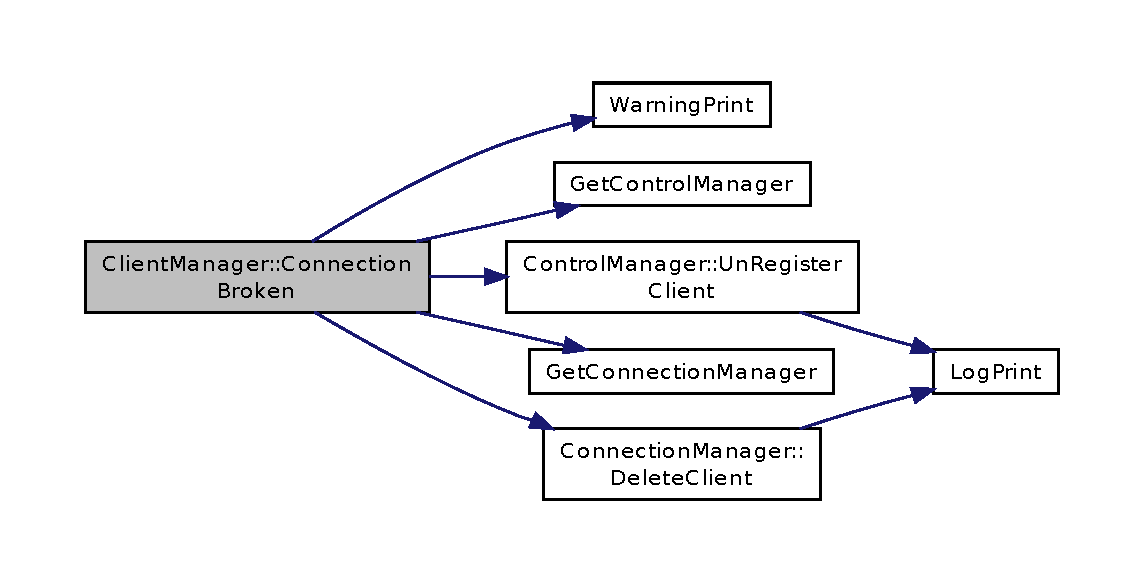
\includegraphics[width=350pt]{class_client_manager_a4fa8fc5731587276f5e6be92563474fa_cgraph}
\end{center}
\end{figure}


\hypertarget{class_client_manager_ab3f0c2bb301ba8d1218d703e5446baf3}{\index{Client\-Manager@{Client\-Manager}!Is\-Asynchronous@{Is\-Asynchronous}}
\index{Is\-Asynchronous@{Is\-Asynchronous}!ClientManager@{Client\-Manager}}
\subsubsection[{Is\-Asynchronous}]{\setlength{\rightskip}{0pt plus 5cm}bool Client\-Manager\-::\-Is\-Asynchronous (
\begin{DoxyParamCaption}
\item[{void}]{}
\end{DoxyParamCaption}
) const\hspace{0.3cm}{\ttfamily [inline]}}}\label{class_client_manager_ab3f0c2bb301ba8d1218d703e5446baf3}
Method to check for Asynchronous Client type. \begin{DoxySeeAlso}{See Also}
\hyperlink{class_client_manager_af40c31ade3f23b705bce2a8b3d311ce6}{m\-\_\-client\-Type}
\end{DoxySeeAlso}
\begin{DoxyReturn}{Returns}
Returns whether the client is asynchronous. 
\end{DoxyReturn}


Definition at line 252 of file Client\-Manager.\-h.

\hypertarget{class_client_manager_a626b9383b2b2b7924a1f1e183800fe72}{\index{Client\-Manager@{Client\-Manager}!Is\-Synchronous@{Is\-Synchronous}}
\index{Is\-Synchronous@{Is\-Synchronous}!ClientManager@{Client\-Manager}}
\subsubsection[{Is\-Synchronous}]{\setlength{\rightskip}{0pt plus 5cm}bool Client\-Manager\-::\-Is\-Synchronous (
\begin{DoxyParamCaption}
\item[{void}]{}
\end{DoxyParamCaption}
) const\hspace{0.3cm}{\ttfamily [inline]}}}\label{class_client_manager_a626b9383b2b2b7924a1f1e183800fe72}
Method to check for Synchronous Client type. \begin{DoxySeeAlso}{See Also}
\hyperlink{class_client_manager_af40c31ade3f23b705bce2a8b3d311ce6}{m\-\_\-client\-Type}
\end{DoxySeeAlso}
\begin{DoxyReturn}{Returns}
Returns whether the client is synchronous. 
\end{DoxyReturn}


Definition at line 241 of file Client\-Manager.\-h.

\hypertarget{class_client_manager_abf05d2ac88337dfd02e0b7986ee1e18c}{\index{Client\-Manager@{Client\-Manager}!Message\-Received@{Message\-Received}}
\index{Message\-Received@{Message\-Received}!ClientManager@{Client\-Manager}}
\subsubsection[{Message\-Received}]{\setlength{\rightskip}{0pt plus 5cm}void Client\-Manager\-::\-Message\-Received (
\begin{DoxyParamCaption}
\item[{void $\ast$}]{data, }
\item[{const size\-\_\-t}]{data\-Size}
\end{DoxyParamCaption}
)}}\label{class_client_manager_abf05d2ac88337dfd02e0b7986ee1e18c}


Called when a message is received. 

This function is called by m\-\_\-client when a message is received. It checks for all possible message types and calls the necessary processing method.


\begin{DoxyParams}{Parameters}
{\em data} & Pointer to the received data. \\
\hline
{\em data\-Size} & Size of the received data. \\
\hline
\end{DoxyParams}


Definition at line 70 of file Client\-Manager.\-cpp.



Here is the call graph for this function\-:
\nopagebreak
\begin{figure}[H]
\begin{center}
\leavevmode
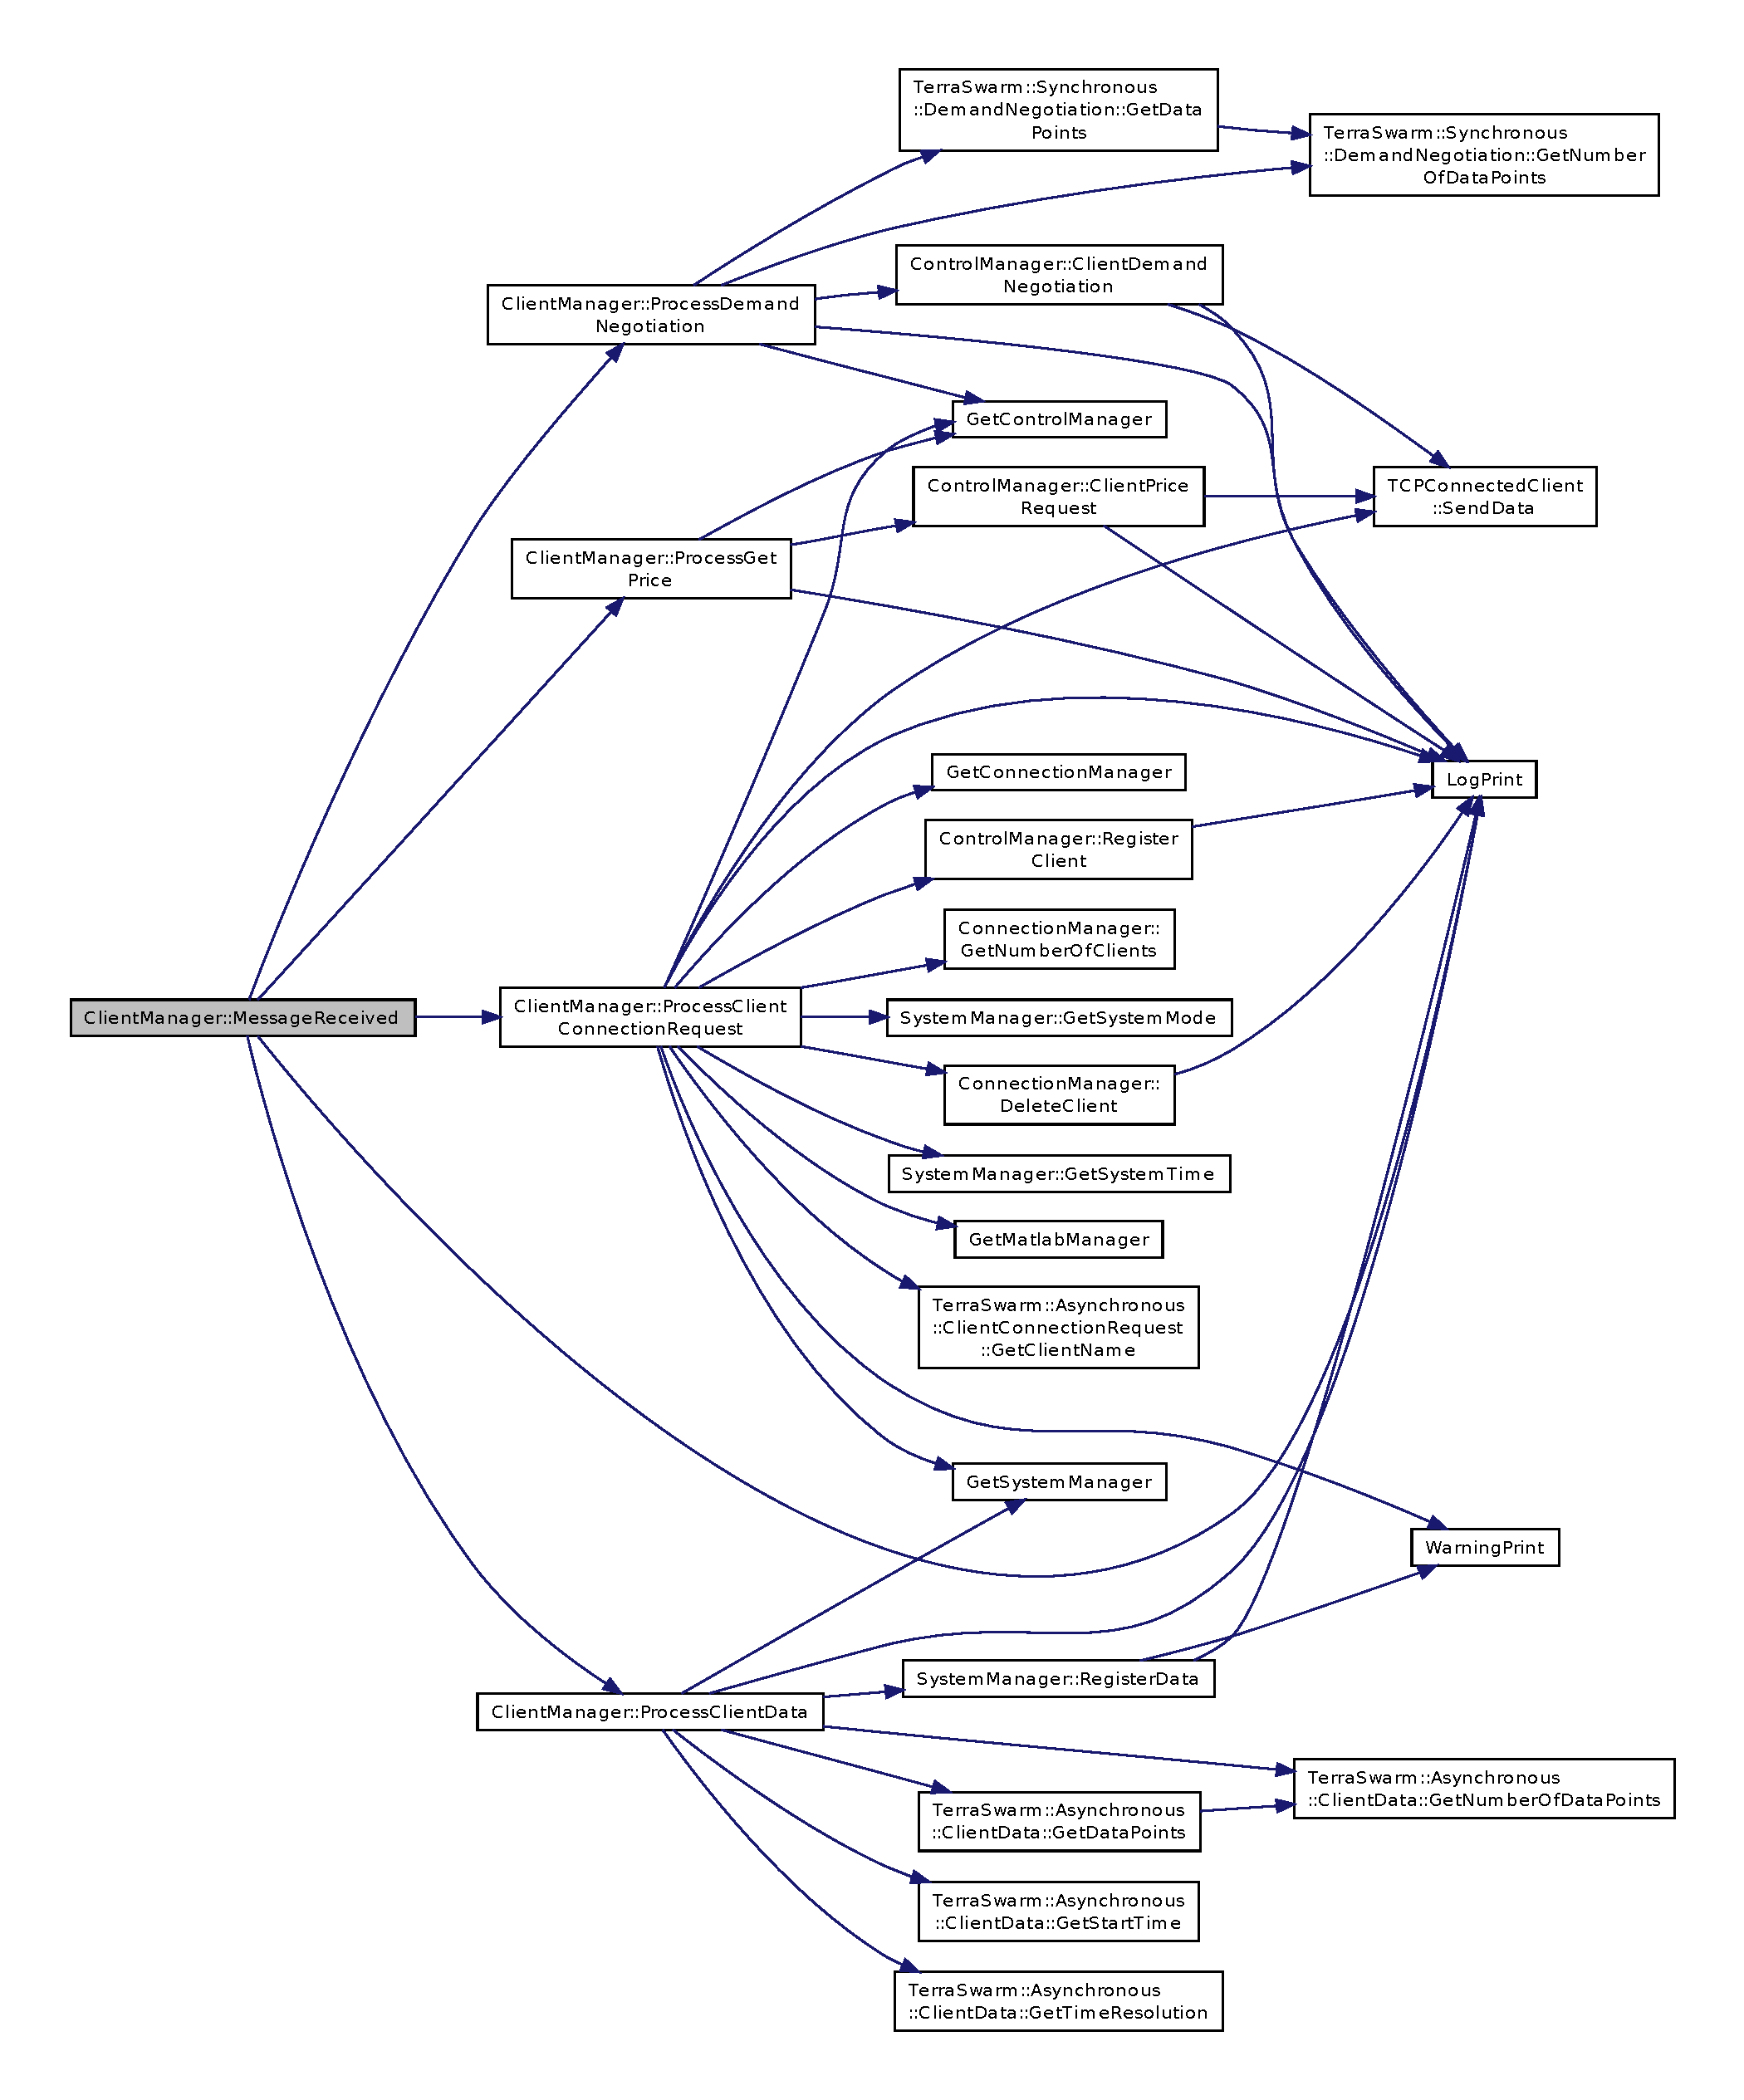
\includegraphics[width=350pt]{class_client_manager_abf05d2ac88337dfd02e0b7986ee1e18c_cgraph}
\end{center}
\end{figure}


\hypertarget{class_client_manager_a1b3ae7dda1e6d1a2939c3eb6a1b9cbd1}{\index{Client\-Manager@{Client\-Manager}!operator=@{operator=}}
\index{operator=@{operator=}!ClientManager@{Client\-Manager}}
\subsubsection[{operator=}]{\setlength{\rightskip}{0pt plus 5cm}{\bf Client\-Manager} \& Client\-Manager\-::operator= (
\begin{DoxyParamCaption}
\item[{const {\bf Client\-Manager} \&}]{copy}
\end{DoxyParamCaption}
)}}\label{class_client_manager_a1b3ae7dda1e6d1a2939c3eb6a1b9cbd1}


Copies the contents of another client manager. 

Overloads the equal operator and copies the content of another client manager.


\begin{DoxyParams}{Parameters}
{\em copy} & Instance to be copied.\\
\hline
\end{DoxyParams}
\begin{DoxyReturn}{Returns}
Returns a reference to itself. 
\end{DoxyReturn}


Definition at line 42 of file Client\-Manager.\-cpp.

\hypertarget{class_client_manager_ae297765312b5f2f93f7b8ec700ad2fbb}{\index{Client\-Manager@{Client\-Manager}!Price\-Proposal@{Price\-Proposal}}
\index{Price\-Proposal@{Price\-Proposal}!ClientManager@{Client\-Manager}}
\subsubsection[{Price\-Proposal}]{\setlength{\rightskip}{0pt plus 5cm}void Client\-Manager\-::\-Price\-Proposal (
\begin{DoxyParamCaption}
\item[{const {\bf T\-Price}}]{price, }
\item[{const {\bf T\-Interval}}]{begin\-Interval, }
\item[{const {\bf T\-Interval}}]{end\-Interval}
\end{DoxyParamCaption}
)}}\label{class_client_manager_ae297765312b5f2f93f7b8ec700ad2fbb}
Sends a price proposal to the client.


\begin{DoxyParams}{Parameters}
{\em price} & Proposed price. \\
\hline
{\em begin\-Interval} & Indicates the beginning time for the proposed price. \\
\hline
{\em end\-Interval} & Indicates the ending time for the proposed price. \\
\hline
\end{DoxyParams}


Definition at line 250 of file Client\-Manager.\-cpp.



Here is the call graph for this function\-:\nopagebreak
\begin{figure}[H]
\begin{center}
\leavevmode
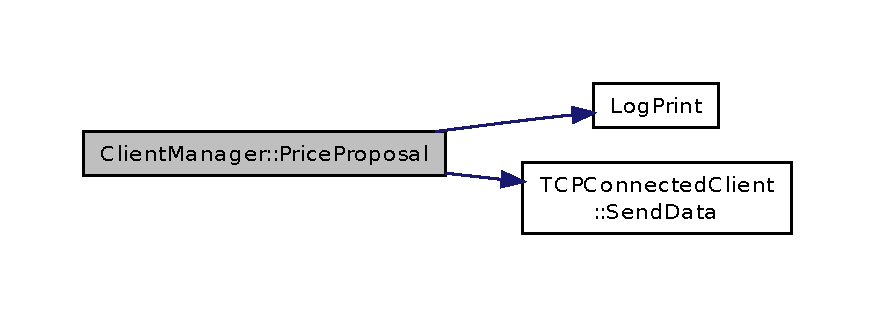
\includegraphics[width=350pt]{class_client_manager_ae297765312b5f2f93f7b8ec700ad2fbb_cgraph}
\end{center}
\end{figure}


\hypertarget{class_client_manager_a6d544b4d20cd3b906b6a033c8d70e4a5}{\index{Client\-Manager@{Client\-Manager}!Process\-Client\-Connection\-Request@{Process\-Client\-Connection\-Request}}
\index{Process\-Client\-Connection\-Request@{Process\-Client\-Connection\-Request}!ClientManager@{Client\-Manager}}
\subsubsection[{Process\-Client\-Connection\-Request}]{\setlength{\rightskip}{0pt plus 5cm}void Client\-Manager\-::\-Process\-Client\-Connection\-Request (
\begin{DoxyParamCaption}
\item[{{\bf Asynchronous\-::\-Client\-Connection\-Request} $\ast$}]{data}
\end{DoxyParamCaption}
)\hspace{0.3cm}{\ttfamily [private]}}}\label{class_client_manager_a6d544b4d20cd3b906b6a033c8d70e4a5}


Processes an asynchronous client connection request. 

This function processes a received asynchronous client connection request. There are multiple steps in the acceptance procedure\-:
\begin{DoxyItemize}
\item Checking with Open\-D\-S\-S whether the object actually exists.
\item If the object exists, an acceptance message is sent back.
\item Next client id is incremented.
\item The client is registered to the \hyperlink{class_control_manager}{Control\-Manager}.
\end{DoxyItemize}


\begin{DoxyParams}{Parameters}
{\em data} & Received message structure in \hyperlink{class_terra_swarm_1_1_asynchronous_1_1_client_connection_request}{Terra\-Swarm\-::\-Asynchronous\-::\-Client\-Connection\-Request}. \\
\hline
\end{DoxyParams}


Definition at line 108 of file Client\-Manager.\-cpp.



Here is the call graph for this function\-:
\nopagebreak
\begin{figure}[H]
\begin{center}
\leavevmode
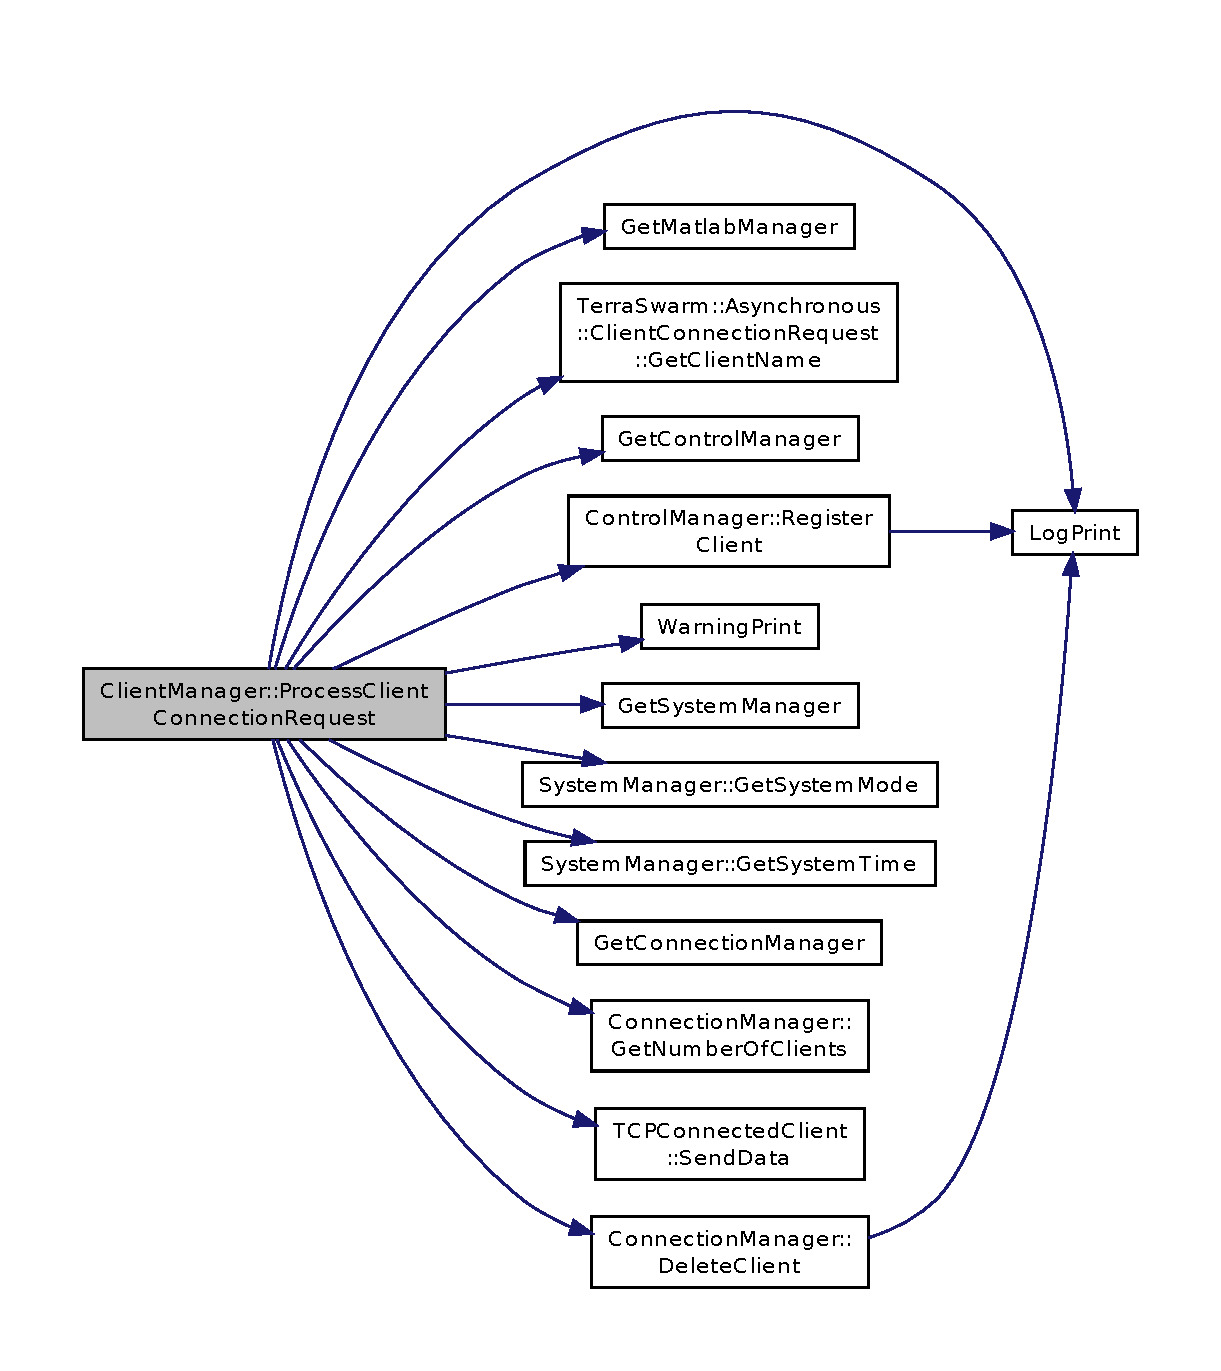
\includegraphics[width=350pt]{class_client_manager_a6d544b4d20cd3b906b6a033c8d70e4a5_cgraph}
\end{center}
\end{figure}




Here is the caller graph for this function\-:\nopagebreak
\begin{figure}[H]
\begin{center}
\leavevmode
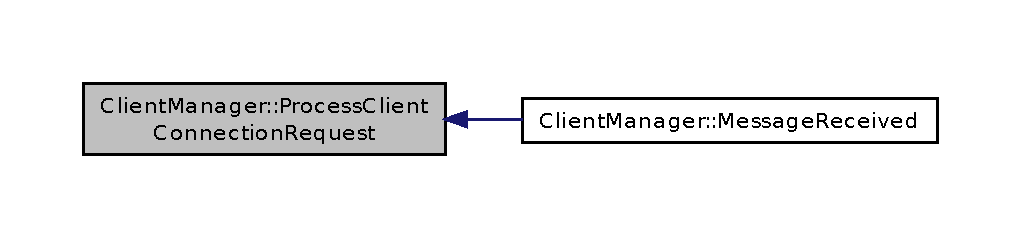
\includegraphics[width=350pt]{class_client_manager_a6d544b4d20cd3b906b6a033c8d70e4a5_icgraph}
\end{center}
\end{figure}


\hypertarget{class_client_manager_aeaa1090897b231a37c7e61b4f95067d1}{\index{Client\-Manager@{Client\-Manager}!Process\-Client\-Connection\-Request@{Process\-Client\-Connection\-Request}}
\index{Process\-Client\-Connection\-Request@{Process\-Client\-Connection\-Request}!ClientManager@{Client\-Manager}}
\subsubsection[{Process\-Client\-Connection\-Request}]{\setlength{\rightskip}{0pt plus 5cm}void Client\-Manager\-::\-Process\-Client\-Connection\-Request (
\begin{DoxyParamCaption}
\item[{{\bf Synchronous\-::\-Client\-Connection\-Request} $\ast$}]{data}
\end{DoxyParamCaption}
)\hspace{0.3cm}{\ttfamily [private]}}}\label{class_client_manager_aeaa1090897b231a37c7e61b4f95067d1}


Processes an synchronous client connection request. 

This function processes a received synchronous client connection request. There are multiple steps in the acceptance procedure\-:
\begin{DoxyItemize}
\item Checking with Open\-D\-S\-S whether the object actually exists.
\item If the object exists, an acceptance message is sent back.
\item Next client id is incremented.
\item The client is registered to the \hyperlink{class_control_manager}{Control\-Manager}.
\end{DoxyItemize}


\begin{DoxyParams}{Parameters}
{\em data} & Received message structure in \hyperlink{class_terra_swarm_1_1_synchronous_1_1_client_connection_request}{Terra\-Swarm\-::\-Synchronous\-::\-Client\-Connection\-Request}. \\
\hline
\end{DoxyParams}


Definition at line 163 of file Client\-Manager.\-cpp.



Here is the call graph for this function\-:
\nopagebreak
\begin{figure}[H]
\begin{center}
\leavevmode
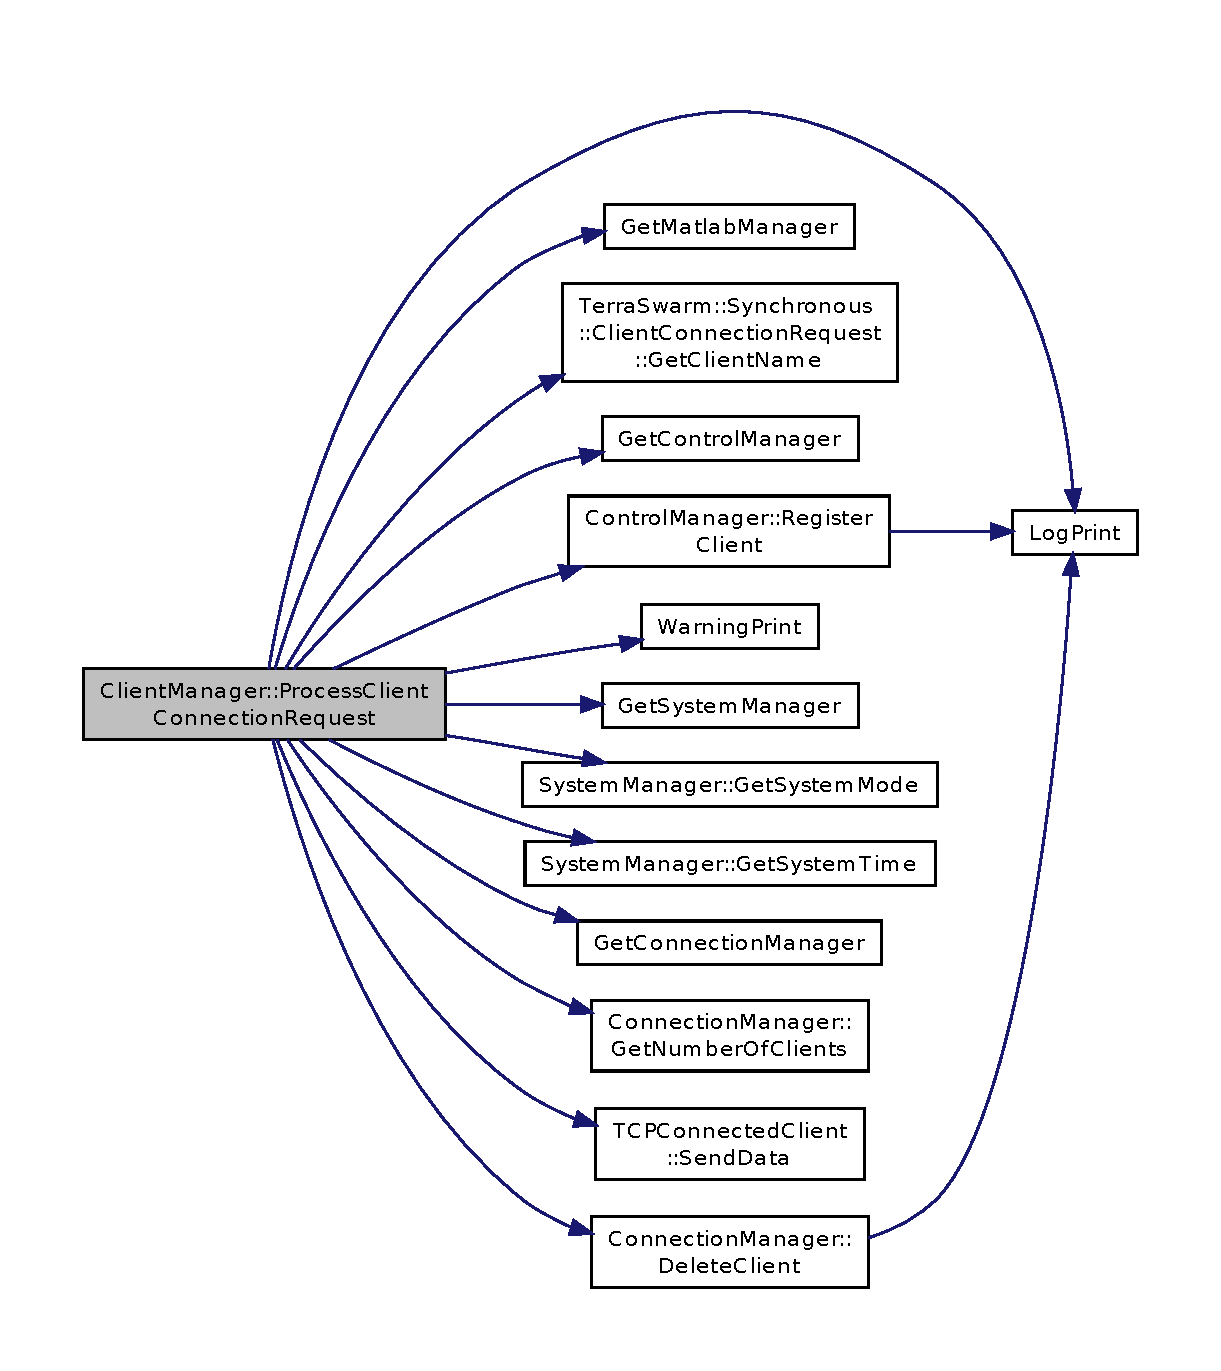
\includegraphics[width=350pt]{class_client_manager_aeaa1090897b231a37c7e61b4f95067d1_cgraph}
\end{center}
\end{figure}


\hypertarget{class_client_manager_a1dd815fe845945ae8966b3a3f449ba0e}{\index{Client\-Manager@{Client\-Manager}!Process\-Client\-Data@{Process\-Client\-Data}}
\index{Process\-Client\-Data@{Process\-Client\-Data}!ClientManager@{Client\-Manager}}
\subsubsection[{Process\-Client\-Data}]{\setlength{\rightskip}{0pt plus 5cm}void Client\-Manager\-::\-Process\-Client\-Data (
\begin{DoxyParamCaption}
\item[{{\bf Asynchronous\-::\-Client\-Data} $\ast$}]{data}
\end{DoxyParamCaption}
)\hspace{0.3cm}{\ttfamily [private]}}}\label{class_client_manager_a1dd815fe845945ae8966b3a3f449ba0e}


Processes the consumption information. 

This function processes the received consumption information of the asynchronous client. The data is registered to the \hyperlink{class_system_manager}{System\-Manager}.


\begin{DoxyParams}{Parameters}
{\em data} & Received message structure in \hyperlink{class_terra_swarm_1_1_asynchronous_1_1_client_data}{Terra\-Swarm\-::\-Asynchronous\-::\-Client\-Data}. \\
\hline
\end{DoxyParams}


Definition at line 150 of file Client\-Manager.\-cpp.



Here is the call graph for this function\-:\nopagebreak
\begin{figure}[H]
\begin{center}
\leavevmode
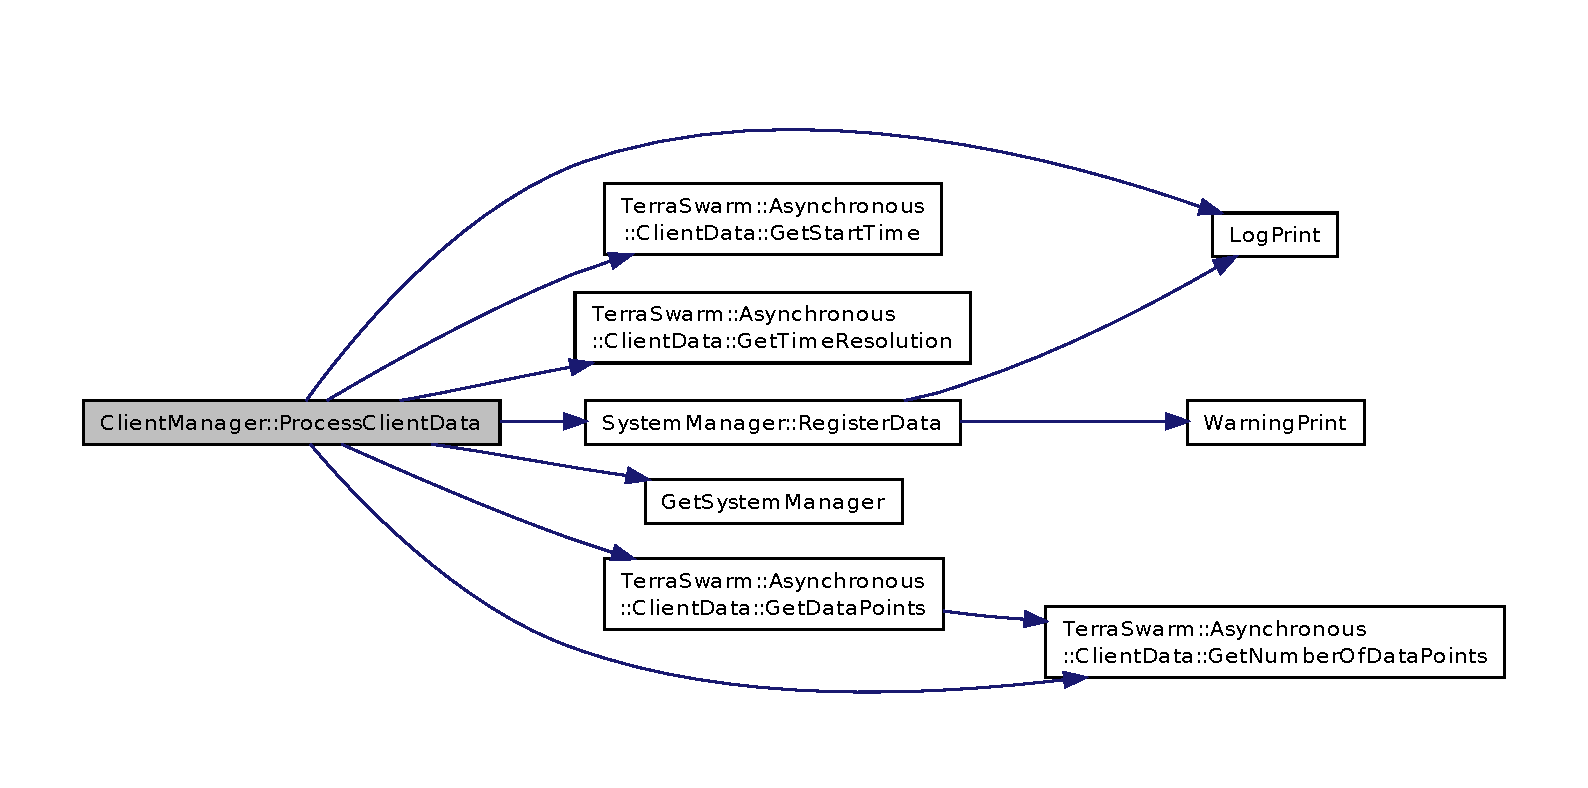
\includegraphics[width=350pt]{class_client_manager_a1dd815fe845945ae8966b3a3f449ba0e_cgraph}
\end{center}
\end{figure}




Here is the caller graph for this function\-:\nopagebreak
\begin{figure}[H]
\begin{center}
\leavevmode
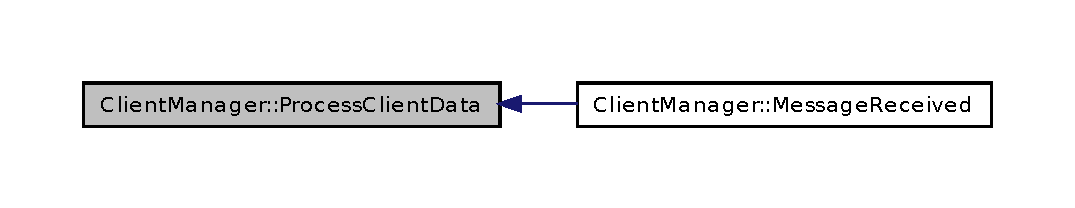
\includegraphics[width=350pt]{class_client_manager_a1dd815fe845945ae8966b3a3f449ba0e_icgraph}
\end{center}
\end{figure}


\hypertarget{class_client_manager_a1d7fd8ecff3bc921273e2928693e4c7d}{\index{Client\-Manager@{Client\-Manager}!Process\-Client\-Data@{Process\-Client\-Data}}
\index{Process\-Client\-Data@{Process\-Client\-Data}!ClientManager@{Client\-Manager}}
\subsubsection[{Process\-Client\-Data}]{\setlength{\rightskip}{0pt plus 5cm}void Client\-Manager\-::\-Process\-Client\-Data (
\begin{DoxyParamCaption}
\item[{{\bf Synchronous\-::\-Client\-Data} $\ast$}]{data}
\end{DoxyParamCaption}
)\hspace{0.3cm}{\ttfamily [private]}}}\label{class_client_manager_a1d7fd8ecff3bc921273e2928693e4c7d}


Processes the consumption information. 

This function processes the received consumption information of the synchronous client. The data is registered to the \hyperlink{class_system_manager}{System\-Manager}.


\begin{DoxyParams}{Parameters}
{\em data} & Received message structure in Terra\-Swarm\-Synchronous\-::\-Client\-Data. \\
\hline
\end{DoxyParams}


Definition at line 204 of file Client\-Manager.\-cpp.



Here is the call graph for this function\-:\nopagebreak
\begin{figure}[H]
\begin{center}
\leavevmode
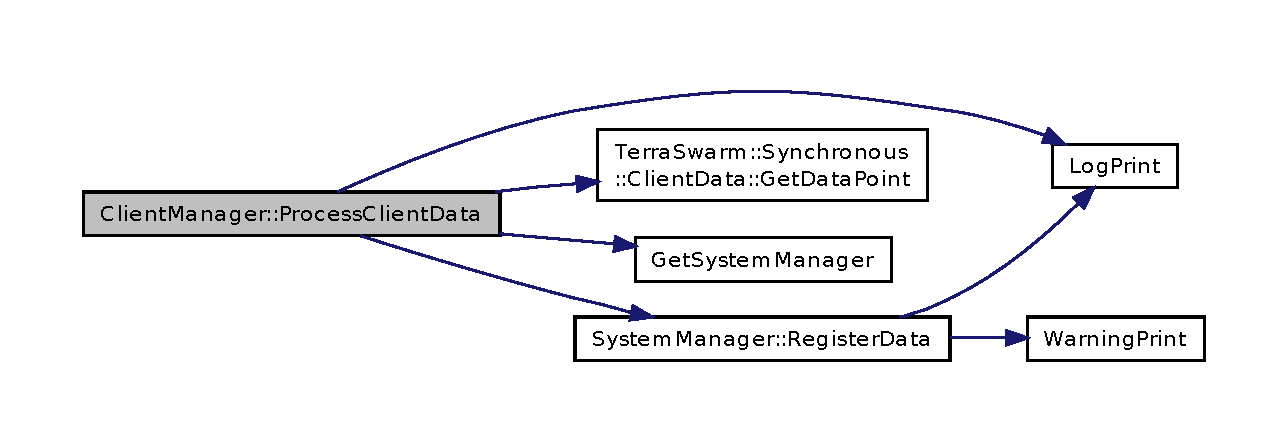
\includegraphics[width=350pt]{class_client_manager_a1d7fd8ecff3bc921273e2928693e4c7d_cgraph}
\end{center}
\end{figure}


\hypertarget{class_client_manager_ad8841acd386513f41ab0872c67593ff4}{\index{Client\-Manager@{Client\-Manager}!Process\-Demand\-Negotiation@{Process\-Demand\-Negotiation}}
\index{Process\-Demand\-Negotiation@{Process\-Demand\-Negotiation}!ClientManager@{Client\-Manager}}
\subsubsection[{Process\-Demand\-Negotiation}]{\setlength{\rightskip}{0pt plus 5cm}void Client\-Manager\-::\-Process\-Demand\-Negotiation (
\begin{DoxyParamCaption}
\item[{{\bf Synchronous\-::\-Demand\-Negotiation} $\ast$}]{data}
\end{DoxyParamCaption}
)\hspace{0.3cm}{\ttfamily [private]}}}\label{class_client_manager_ad8841acd386513f41ab0872c67593ff4}


Processes the demand negotiation response. 

The client sends a demand negotiation response to the simulator. This response is sent to \hyperlink{class_control_manager}{Control\-Manager}.


\begin{DoxyParams}{Parameters}
{\em data} & Received message structure in \hyperlink{class_terra_swarm_1_1_synchronous_1_1_demand_negotiation}{Terra\-Swarm\-::\-Synchronous\-::\-Demand\-Negotiation}. \\
\hline
\end{DoxyParams}


Definition at line 223 of file Client\-Manager.\-cpp.



Here is the call graph for this function\-:
\nopagebreak
\begin{figure}[H]
\begin{center}
\leavevmode
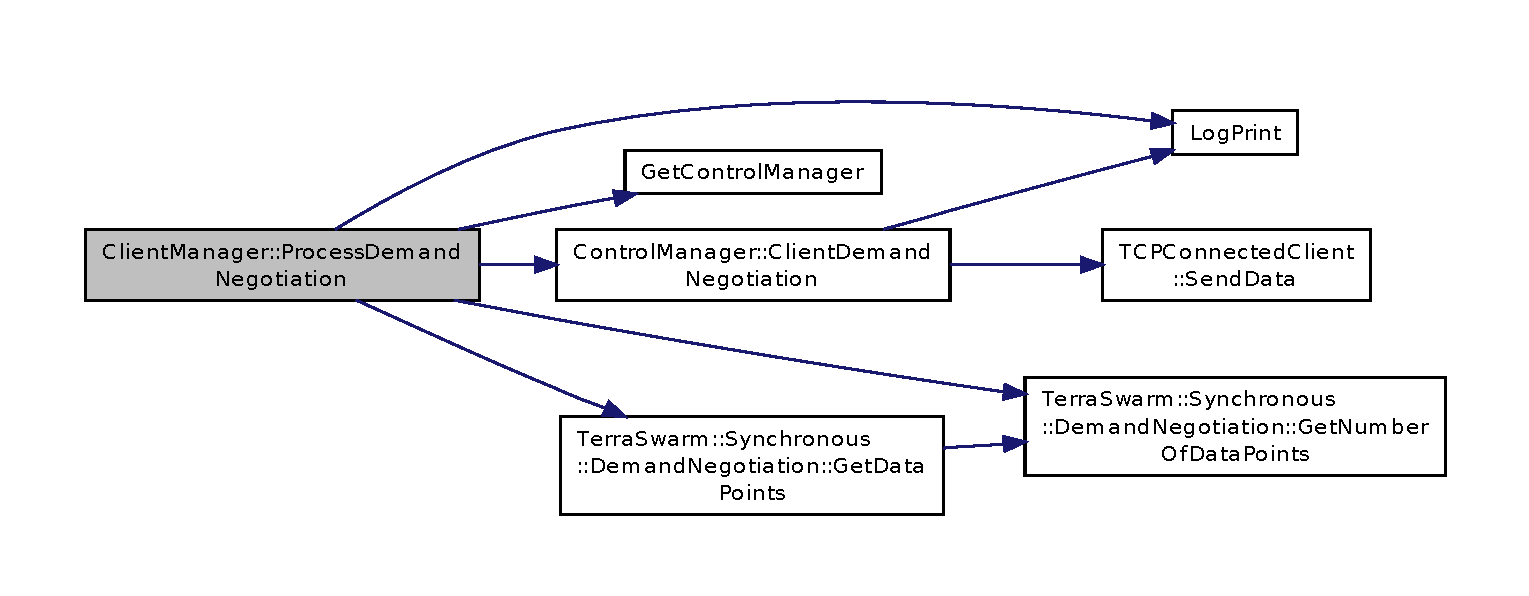
\includegraphics[width=350pt]{class_client_manager_ad8841acd386513f41ab0872c67593ff4_cgraph}
\end{center}
\end{figure}




Here is the caller graph for this function\-:\nopagebreak
\begin{figure}[H]
\begin{center}
\leavevmode
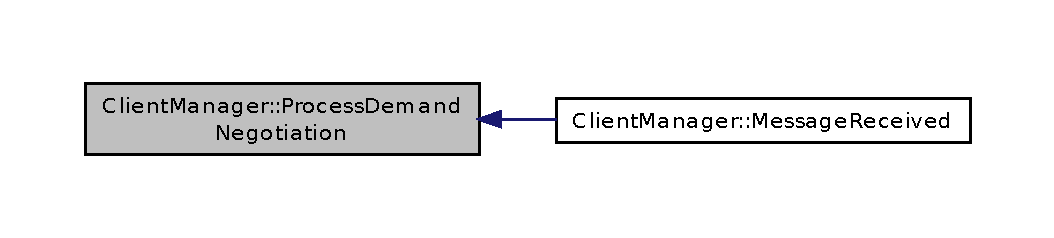
\includegraphics[width=350pt]{class_client_manager_ad8841acd386513f41ab0872c67593ff4_icgraph}
\end{center}
\end{figure}


\hypertarget{class_client_manager_a841299387a1dcd268266a3c0cfe2a95c}{\index{Client\-Manager@{Client\-Manager}!Process\-Get\-Price@{Process\-Get\-Price}}
\index{Process\-Get\-Price@{Process\-Get\-Price}!ClientManager@{Client\-Manager}}
\subsubsection[{Process\-Get\-Price}]{\setlength{\rightskip}{0pt plus 5cm}void Client\-Manager\-::\-Process\-Get\-Price (
\begin{DoxyParamCaption}
\item[{{\bf Synchronous\-::\-Get\-Price} $\ast$}]{data}
\end{DoxyParamCaption}
)\hspace{0.3cm}{\ttfamily [private]}}}\label{class_client_manager_a841299387a1dcd268266a3c0cfe2a95c}


Processes the price signal request. 

The price signal request by the synchronous client is sent to \hyperlink{class_control_manager}{Control\-Manager}. 
\begin{DoxyParams}{Parameters}
{\em data} & Received message structure in \hyperlink{class_terra_swarm_1_1_synchronous_1_1_get_price}{Terra\-Swarm\-::\-Synchronous\-::\-Get\-Price}. \\
\hline
\end{DoxyParams}


Definition at line 214 of file Client\-Manager.\-cpp.



Here is the call graph for this function\-:
\nopagebreak
\begin{figure}[H]
\begin{center}
\leavevmode
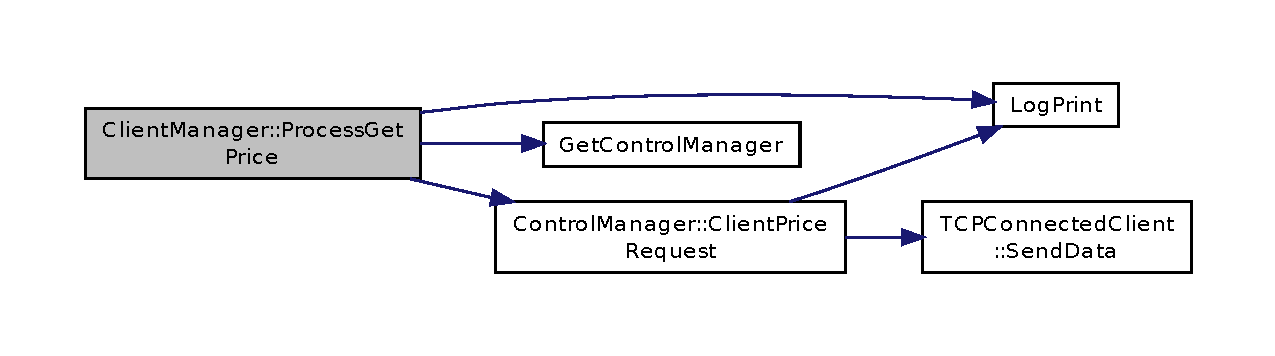
\includegraphics[width=350pt]{class_client_manager_a841299387a1dcd268266a3c0cfe2a95c_cgraph}
\end{center}
\end{figure}




Here is the caller graph for this function\-:\nopagebreak
\begin{figure}[H]
\begin{center}
\leavevmode
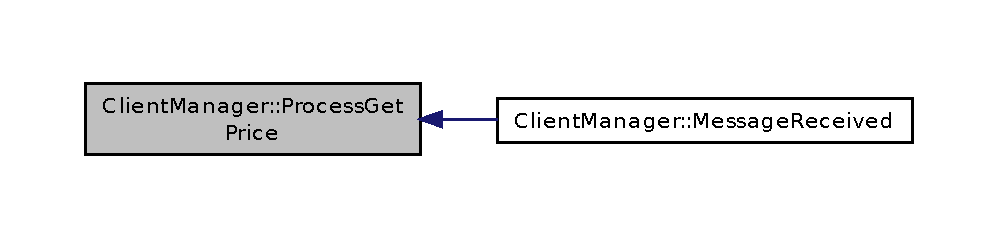
\includegraphics[width=350pt]{class_client_manager_a841299387a1dcd268266a3c0cfe2a95c_icgraph}
\end{center}
\end{figure}


\hypertarget{class_client_manager_adb64a2ee5d0eb7b1a4bdedcd0e3b92f5}{\index{Client\-Manager@{Client\-Manager}!Set\-Current\-Price@{Set\-Current\-Price}}
\index{Set\-Current\-Price@{Set\-Current\-Price}!ClientManager@{Client\-Manager}}
\subsubsection[{Set\-Current\-Price}]{\setlength{\rightskip}{0pt plus 5cm}void Client\-Manager\-::\-Set\-Current\-Price (
\begin{DoxyParamCaption}
\item[{const {\bf T\-Price}}]{price, }
\item[{const {\bf T\-Interval}}]{begin\-Interval, }
\item[{const {\bf T\-Interval}}]{end\-Interval}
\end{DoxyParamCaption}
)}}\label{class_client_manager_adb64a2ee5d0eb7b1a4bdedcd0e3b92f5}
Sends a price signal to the client.


\begin{DoxyParams}{Parameters}
{\em price} & Indicates the price. \\
\hline
{\em begin\-Interval} & Indicates the beginning time for the price. \\
\hline
{\em end\-Interval} & Indicates the ending time for the price. \\
\hline
\end{DoxyParams}


Definition at line 234 of file Client\-Manager.\-cpp.



Here is the call graph for this function\-:\nopagebreak
\begin{figure}[H]
\begin{center}
\leavevmode
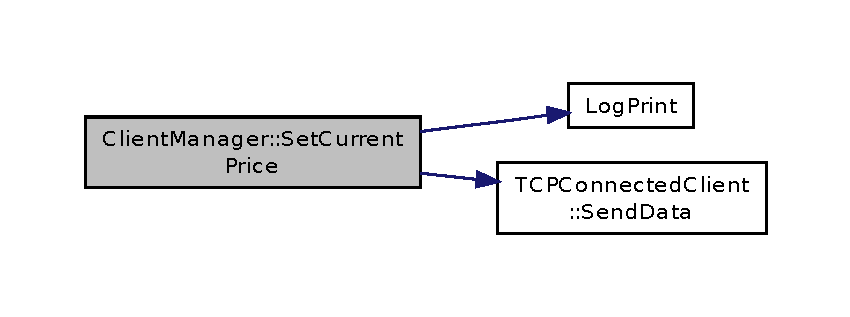
\includegraphics[width=350pt]{class_client_manager_adb64a2ee5d0eb7b1a4bdedcd0e3b92f5_cgraph}
\end{center}
\end{figure}




\subsection{Member Data Documentation}
\hypertarget{class_client_manager_a86ae04f2ac9f2988559a023d877f78e4}{\index{Client\-Manager@{Client\-Manager}!m\-\_\-client@{m\-\_\-client}}
\index{m\-\_\-client@{m\-\_\-client}!ClientManager@{Client\-Manager}}
\subsubsection[{m\-\_\-client}]{\setlength{\rightskip}{0pt plus 5cm}{\bf Threaded\-T\-C\-P\-Connected\-Client}$\ast$ Client\-Manager\-::m\-\_\-client\hspace{0.3cm}{\ttfamily [private]}}}\label{class_client_manager_a86ae04f2ac9f2988559a023d877f78e4}
Pointer to the T\-C\-P Client connection managing class instance. This variable is used for all communication purposes. 

Definition at line 75 of file Client\-Manager.\-h.

\hypertarget{class_client_manager_a1216ffa88107c33825adafe63fea2263}{\index{Client\-Manager@{Client\-Manager}!m\-\_\-client\-Id@{m\-\_\-client\-Id}}
\index{m\-\_\-client\-Id@{m\-\_\-client\-Id}!ClientManager@{Client\-Manager}}
\subsubsection[{m\-\_\-client\-Id}]{\setlength{\rightskip}{0pt plus 5cm}{\bf T\-Id} Client\-Manager\-::m\-\_\-client\-Id\hspace{0.3cm}{\ttfamily [private]}}}\label{class_client_manager_a1216ffa88107c33825adafe63fea2263}
Actual assigned Unique I\-D of the managed client. 

Definition at line 79 of file Client\-Manager.\-h.

\hypertarget{class_client_manager_af40c31ade3f23b705bce2a8b3d311ce6}{\index{Client\-Manager@{Client\-Manager}!m\-\_\-client\-Type@{m\-\_\-client\-Type}}
\index{m\-\_\-client\-Type@{m\-\_\-client\-Type}!ClientManager@{Client\-Manager}}
\subsubsection[{m\-\_\-client\-Type}]{\setlength{\rightskip}{0pt plus 5cm}{\bf T\-Client\-Type} Client\-Manager\-::m\-\_\-client\-Type\hspace{0.3cm}{\ttfamily [private]}}}\label{class_client_manager_af40c31ade3f23b705bce2a8b3d311ce6}
Type of the managed client. \begin{DoxySeeAlso}{See Also}
\{\hyperlink{class_client_manager_ac12239be9a30847f677a32910822d40b}{Client\-Manager\-::\-Client\-Type\-Values}\} 
\end{DoxySeeAlso}


Definition at line 83 of file Client\-Manager.\-h.

\hypertarget{class_client_manager_a4f044df4d9f43367135f9d01841ec326}{\index{Client\-Manager@{Client\-Manager}!next\-Client\-Id@{next\-Client\-Id}}
\index{next\-Client\-Id@{next\-Client\-Id}!ClientManager@{Client\-Manager}}
\subsubsection[{next\-Client\-Id}]{\setlength{\rightskip}{0pt plus 5cm}{\bf Client\-Manager\-::\-T\-Id} Client\-Manager\-::next\-Client\-Id = 1\hspace{0.3cm}{\ttfamily [static]}, {\ttfamily [private]}}}\label{class_client_manager_a4f044df4d9f43367135f9d01841ec326}
Static variable that holds the next Unique I\-D. Incremented at each new connection. Returns to 0 if all values have been used. 

Definition at line 71 of file Client\-Manager.\-h.



The documentation for this class was generated from the following files\-:\begin{DoxyCompactItemize}
\item 
S2\-Sim/\hyperlink{_client_manager_8h}{Client\-Manager.\-h}\item 
S2\-Sim/\hyperlink{_client_manager_8cpp}{Client\-Manager.\-cpp}\end{DoxyCompactItemize}

\hypertarget{class_compile_check}{\section{Compile\-Check$<$ expression, Reason $>$ Class Template Reference}
\label{class_compile_check}\index{Compile\-Check$<$ expression, Reason $>$@{Compile\-Check$<$ expression, Reason $>$}}
}


{\ttfamily \#include $<$Compile\-Time\-Checker\-Library.\-h$>$}

\subsection*{Public Types}
\begin{DoxyCompactItemize}
\item 
enum \{ \hyperlink{class_compile_check_a23f09425353e49afb718c608ee4e14eeae1aaa6a952694dd245ce18936fb2b758}{Result} = true
 \}
\end{DoxyCompactItemize}
\subsection*{Static Public Member Functions}
\begin{DoxyCompactItemize}
\item 
static void \hyperlink{class_compile_check_a0b48338cd3cb0e57b5d5182a1400f847}{Check} (void)
\end{DoxyCompactItemize}


\subsection{Detailed Description}
\subsubsection*{template$<$bool expression, typename Reason = class No\-Reason$>$class Compile\-Check$<$ expression, Reason $>$}



Definition at line 12 of file Compile\-Time\-Checker\-Library.\-h.



\subsection{Member Enumeration Documentation}
\hypertarget{class_compile_check_a23f09425353e49afb718c608ee4e14ee}{\subsubsection[{anonymous enum}]{\setlength{\rightskip}{0pt plus 5cm}template$<$bool expression, typename Reason  = class No\-Reason$>$ anonymous enum}}\label{class_compile_check_a23f09425353e49afb718c608ee4e14ee}
\begin{Desc}
\item[Enumerator]\par
\begin{description}
\index{Result@{Result}!Compile\-Check@{Compile\-Check}}\index{Compile\-Check@{Compile\-Check}!Result@{Result}}\item[{\em 
\hypertarget{class_compile_check_a23f09425353e49afb718c608ee4e14eeae1aaa6a952694dd245ce18936fb2b758}{Result}\label{class_compile_check_a23f09425353e49afb718c608ee4e14eeae1aaa6a952694dd245ce18936fb2b758}
}]\end{description}
\end{Desc}


Definition at line 15 of file Compile\-Time\-Checker\-Library.\-h.



\subsection{Member Function Documentation}
\hypertarget{class_compile_check_a0b48338cd3cb0e57b5d5182a1400f847}{\index{Compile\-Check@{Compile\-Check}!Check@{Check}}
\index{Check@{Check}!CompileCheck@{Compile\-Check}}
\subsubsection[{Check}]{\setlength{\rightskip}{0pt plus 5cm}template$<$bool expression, typename Reason  = class No\-Reason$>$ static void {\bf Compile\-Check}$<$ expression, Reason $>$\-::Check (
\begin{DoxyParamCaption}
\item[{void}]{}
\end{DoxyParamCaption}
)\hspace{0.3cm}{\ttfamily [inline]}, {\ttfamily [static]}}}\label{class_compile_check_a0b48338cd3cb0e57b5d5182a1400f847}


Definition at line 20 of file Compile\-Time\-Checker\-Library.\-h.



The documentation for this class was generated from the following file\-:\begin{DoxyCompactItemize}
\item 
S2\-Sim/\-Terraswarm\-Library/\hyperlink{_compile_time_checker_library_8h}{Compile\-Time\-Checker\-Library.\-h}\end{DoxyCompactItemize}

\hypertarget{class_compile_check_3_01false_00_01_reason_01_4}{\section{Compile\-Check$<$ false, Reason $>$ Class Template Reference}
\label{class_compile_check_3_01false_00_01_reason_01_4}\index{Compile\-Check$<$ false, Reason $>$@{Compile\-Check$<$ false, Reason $>$}}
}


Second specialization of the class, when the expression is not true.  




{\ttfamily \#include $<$Compile\-Time\-Checker\-Library.\-h$>$}

\subsection*{Private Types}
\begin{DoxyCompactItemize}
\item 
enum \{ \hyperlink{class_compile_check_3_01false_00_01_reason_01_4_a7777002f83cd288663fad3eba2721a9ba9f7df94908ad6f5f6296d4bb2e8e0e3f}{Result} = true
 \}
\begin{DoxyCompactList}\small\item\em Enumeration for Result displaying. \end{DoxyCompactList}\end{DoxyCompactItemize}
\subsection*{Static Private Member Functions}
\begin{DoxyCompactItemize}
\item 
static void \hyperlink{class_compile_check_3_01false_00_01_reason_01_4_a1da45a656d0ba16e65e757aa3492c1da}{Check} (void)
\begin{DoxyCompactList}\small\item\em Empty function for visual purposes. \end{DoxyCompactList}\end{DoxyCompactItemize}


\subsection{Detailed Description}
\subsubsection*{template$<$typename Reason$>$class Compile\-Check$<$ false, Reason $>$}

Second specialization of the class, when the expression is not true. 

The static \hyperlink{class_compile_check_3_01false_00_01_reason_01_4_a1da45a656d0ba16e65e757aa3492c1da}{Check()} function is this time private and the compilation will fail. 

Definition at line 43 of file Compile\-Time\-Checker\-Library.\-h.



\subsection{Member Enumeration Documentation}
\hypertarget{class_compile_check_3_01false_00_01_reason_01_4_a7777002f83cd288663fad3eba2721a9b}{\subsubsection[{anonymous enum}]{\setlength{\rightskip}{0pt plus 5cm}template$<$typename Reason $>$ anonymous enum\hspace{0.3cm}{\ttfamily [private]}}}\label{class_compile_check_3_01false_00_01_reason_01_4_a7777002f83cd288663fad3eba2721a9b}


Enumeration for Result displaying. 

\begin{Desc}
\item[Enumerator]\par
\begin{description}
\index{Result@{Result}!Compile\-Check$<$ false, Reason $>$@{Compile\-Check$<$ false, Reason $>$}}\index{Compile\-Check$<$ false, Reason $>$@{Compile\-Check$<$ false, Reason $>$}!Result@{Result}}\item[{\em 
\hypertarget{class_compile_check_3_01false_00_01_reason_01_4_a7777002f83cd288663fad3eba2721a9ba9f7df94908ad6f5f6296d4bb2e8e0e3f}{Result}\label{class_compile_check_3_01false_00_01_reason_01_4_a7777002f83cd288663fad3eba2721a9ba9f7df94908ad6f5f6296d4bb2e8e0e3f}
}]The check has failed. \end{description}
\end{Desc}


Definition at line 49 of file Compile\-Time\-Checker\-Library.\-h.



\subsection{Member Function Documentation}
\hypertarget{class_compile_check_3_01false_00_01_reason_01_4_a1da45a656d0ba16e65e757aa3492c1da}{\index{Compile\-Check$<$ false, Reason $>$@{Compile\-Check$<$ false, Reason $>$}!Check@{Check}}
\index{Check@{Check}!CompileCheck< false, Reason >@{Compile\-Check$<$ false, Reason $>$}}
\subsubsection[{Check}]{\setlength{\rightskip}{0pt plus 5cm}template$<$typename Reason $>$ static void {\bf Compile\-Check}$<$ false, Reason $>$\-::Check (
\begin{DoxyParamCaption}
\item[{void}]{}
\end{DoxyParamCaption}
)\hspace{0.3cm}{\ttfamily [inline]}, {\ttfamily [static]}, {\ttfamily [private]}}}\label{class_compile_check_3_01false_00_01_reason_01_4_a1da45a656d0ba16e65e757aa3492c1da}


Empty function for visual purposes. 



Definition at line 60 of file Compile\-Time\-Checker\-Library.\-h.



The documentation for this class was generated from the following file\-:\begin{DoxyCompactItemize}
\item 
S2\-Sim/\-Terraswarm\-Library/\hyperlink{_compile_time_checker_library_8h}{Compile\-Time\-Checker\-Library.\-h}\end{DoxyCompactItemize}

\hypertarget{class_connection_manager}{\section{Connection\-Manager Class Reference}
\label{class_connection_manager}\index{Connection\-Manager@{Connection\-Manager}}
}


Manages connections to all clients.  




{\ttfamily \#include $<$Connection\-Manager.\-h$>$}



Collaboration diagram for Connection\-Manager\-:\nopagebreak
\begin{figure}[H]
\begin{center}
\leavevmode
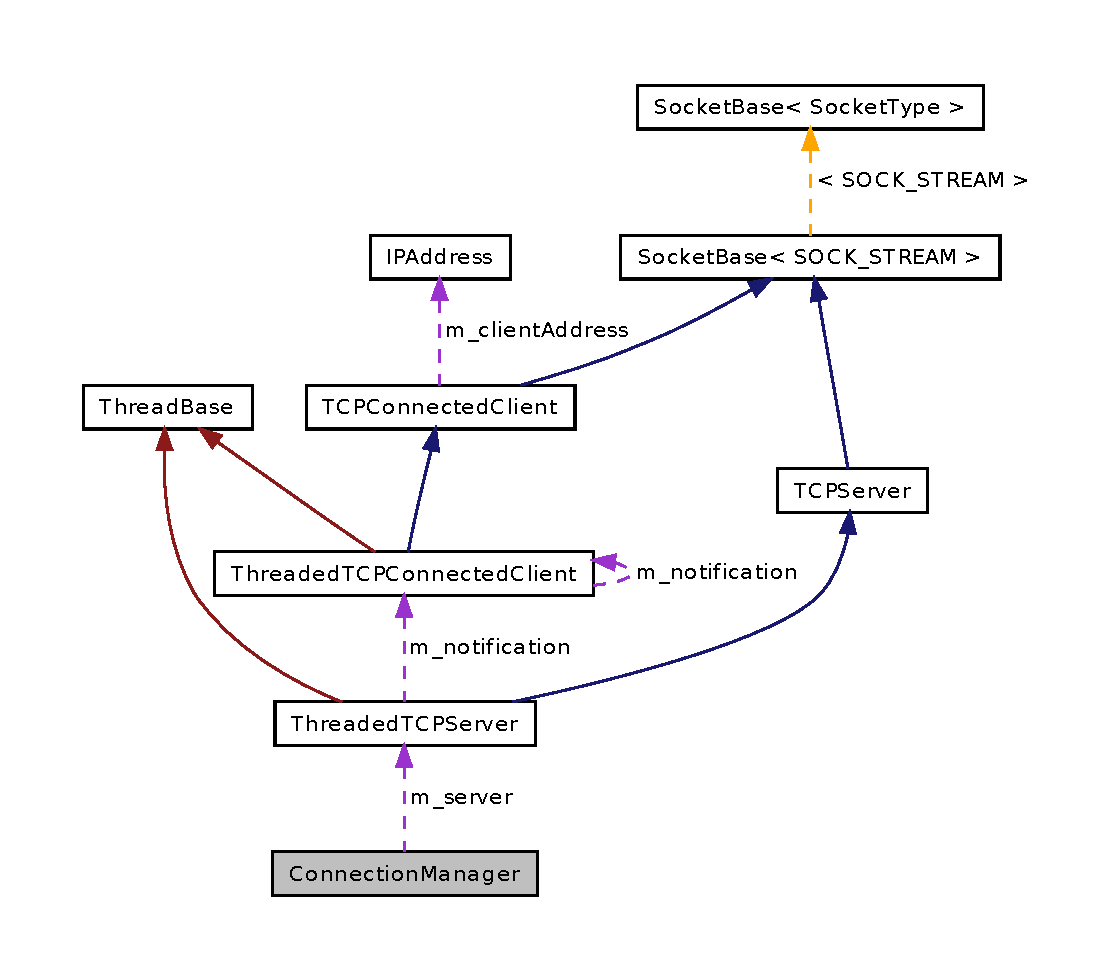
\includegraphics[width=350pt]{class_connection_manager__coll__graph}
\end{center}
\end{figure}
\subsection*{Public Types}
\begin{DoxyCompactItemize}
\item 
typedef \hyperlink{class_connection_manager_a0c3634c02b95af84a477b253fcf2b29a}{T\-Client\-Id} \hyperlink{class_connection_manager_a0f5f5b25b063cfebfac54b25cda131f7}{T\-Number\-Of\-Clients}
\begin{DoxyCompactList}\small\item\em Represents the type for number of clients. \end{DoxyCompactList}\end{DoxyCompactItemize}
\subsection*{Public Member Functions}
\begin{DoxyCompactItemize}
\item 
void \hyperlink{class_connection_manager_a54968c1176475aa513538691b75aedc9}{Incoming\-Connection} (\hyperlink{class_threaded_t_c_p_connected_client}{Threaded\-T\-C\-P\-Connected\-Client} $\ast$new\-Client)
\begin{DoxyCompactList}\small\item\em Incoming connection handler. \end{DoxyCompactList}\item 
void \hyperlink{class_connection_manager_a64473b0369ab91daf3a2da6b8ef576d0}{Broken\-Connection} (\hyperlink{class_threaded_t_c_p_connected_client}{Threaded\-T\-C\-P\-Connected\-Client} $\ast$broken\-Client)
\begin{DoxyCompactList}\small\item\em Broken connection handler. \end{DoxyCompactList}\item 
void \hyperlink{class_connection_manager_a4657b51054ad28143f1bddd1f5cc282c}{Incoming\-Message} (\hyperlink{class_threaded_t_c_p_connected_client}{Threaded\-T\-C\-P\-Connected\-Client} $\ast$sender\-Client, void $\ast$buffer, size\-\_\-t size)
\begin{DoxyCompactList}\small\item\em New message processor. \end{DoxyCompactList}\item 
void \hyperlink{class_connection_manager_afc67553cf1eff6ab251a5dd2a313e863}{Delete\-Client} (\hyperlink{class_client_manager}{Client\-Manager} $\ast$client\-Manager)
\begin{DoxyCompactList}\small\item\em Deletes the \hyperlink{class_client_manager}{Client\-Manager} from all lists and finally deletes itself. \end{DoxyCompactList}\item 
\hyperlink{class_connection_manager_a0f5f5b25b063cfebfac54b25cda131f7}{T\-Number\-Of\-Clients} \hyperlink{class_connection_manager_adf13721cde7ae4615aadbb5262f67274}{Get\-Number\-Of\-Clients} (void) const 
\begin{DoxyCompactList}\small\item\em Returns the current number of clients connected. \end{DoxyCompactList}\end{DoxyCompactItemize}
\subsection*{Private Types}
\begin{DoxyCompactItemize}
\item 
typedef \\*
\hyperlink{class_terra_swarm_1_1_message_header_ab55de822fadad758edcd8f36bd07676e}{Terra\-Swarm\-::\-Message\-Header\-::\-T\-Id} \hyperlink{class_connection_manager_a0c3634c02b95af84a477b253fcf2b29a}{T\-Client\-Id}
\begin{DoxyCompactList}\small\item\em Type representing the Unique Id of the client. \end{DoxyCompactList}\item 
typedef std\-::map\\*
$<$ \hyperlink{class_threaded_t_c_p_connected_client}{Threaded\-T\-C\-P\-Connected\-Client} \\*
$\ast$, \hyperlink{class_client_manager}{Client\-Manager} $\ast$ $>$ \hyperlink{class_connection_manager_a7b6865543285e3b27b981a739fd0db18}{T\-Client\-List}
\begin{DoxyCompactList}\small\item\em Type mapping T\-C\-P client connection pointers to their respective managers. \end{DoxyCompactList}\item 
typedef std\-::map\\*
$<$ \hyperlink{class_client_manager}{Client\-Manager} \\*
$\ast$, \hyperlink{class_threaded_t_c_p_connected_client}{Threaded\-T\-C\-P\-Connected\-Client} $\ast$ $>$ \hyperlink{class_connection_manager_aa35cf836145608197dbe4201b115991c}{T\-Reversed\-Client\-List}
\begin{DoxyCompactList}\small\item\em Type mapping the client managers to their respective T\-C\-P client connections. \end{DoxyCompactList}\item 
typedef std\-::map$<$ \hyperlink{class_connection_manager_a0c3634c02b95af84a477b253fcf2b29a}{T\-Client\-Id}, \\*
\hyperlink{class_client_manager}{Client\-Manager} $\ast$ $>$ \hyperlink{class_connection_manager_a78c371deff0ac4add801b3c64216a467}{T\-Client\-Id\-List}
\begin{DoxyCompactList}\small\item\em Type mapping the client unique id's to respective managers. \end{DoxyCompactList}\end{DoxyCompactItemize}
\subsection*{Private Member Functions}
\begin{DoxyCompactItemize}
\item 
\hyperlink{class_connection_manager_a7928f3e95b4e88b01c11eaf3e8089ee7}{Connection\-Manager} (void)
\begin{DoxyCompactList}\small\item\em Private constructor for singleton implementation. \end{DoxyCompactList}\end{DoxyCompactItemize}
\subsection*{Private Attributes}
\begin{DoxyCompactItemize}
\item 
\hyperlink{class_connection_manager_a7b6865543285e3b27b981a739fd0db18}{T\-Client\-List} \hyperlink{class_connection_manager_ad9da7334bc0a1ed0f152f5998b46268a}{m\-\_\-client\-List}
\begin{DoxyCompactList}\small\item\em Holds the Connection-\/$>$Manager based list. \end{DoxyCompactList}\item 
\hyperlink{class_connection_manager_aa35cf836145608197dbe4201b115991c}{T\-Reversed\-Client\-List} \hyperlink{class_connection_manager_aae27a14334d4b84076231534196e75eb}{m\-\_\-reversed\-Client\-List}
\begin{DoxyCompactList}\small\item\em Holds the Manager-\/$>$Connection based list for speed. \end{DoxyCompactList}\item 
\hyperlink{class_threaded_t_c_p_server}{Threaded\-T\-C\-P\-Server} \hyperlink{class_connection_manager_a8858415ddb04364d4697f7ea00aa2977}{m\-\_\-server}
\begin{DoxyCompactList}\small\item\em Instance of the T\-C\-P server. \end{DoxyCompactList}\end{DoxyCompactItemize}
\subsection*{Friends}
\begin{DoxyCompactItemize}
\item 
\hyperlink{class_connection_manager}{Connection\-Manager} \& \hyperlink{class_connection_manager_ab88124ce7a3bf1d2892d0e9763d1af30}{Get\-Connection\-Manager} (void)
\begin{DoxyCompactList}\small\item\em Friend method for singleton implementation. \end{DoxyCompactList}\end{DoxyCompactItemize}


\subsection{Detailed Description}
Manages connections to all clients. 

This class manages the connections to all clients. It implements a T\-C\-P server and answers any connection attempts. It forwards received data to the correct \hyperlink{class_client_manager}{Client\-Manager} instance for processing. 

Definition at line 48 of file Connection\-Manager.\-h.



\subsection{Member Typedef Documentation}
\hypertarget{class_connection_manager_a0c3634c02b95af84a477b253fcf2b29a}{\index{Connection\-Manager@{Connection\-Manager}!T\-Client\-Id@{T\-Client\-Id}}
\index{T\-Client\-Id@{T\-Client\-Id}!ConnectionManager@{Connection\-Manager}}
\subsubsection[{T\-Client\-Id}]{\setlength{\rightskip}{0pt plus 5cm}typedef {\bf Terra\-Swarm\-::\-Message\-Header\-::\-T\-Id} {\bf Connection\-Manager\-::\-T\-Client\-Id}\hspace{0.3cm}{\ttfamily [private]}}}\label{class_connection_manager_a0c3634c02b95af84a477b253fcf2b29a}


Type representing the Unique Id of the client. 



Definition at line 62 of file Connection\-Manager.\-h.

\hypertarget{class_connection_manager_a78c371deff0ac4add801b3c64216a467}{\index{Connection\-Manager@{Connection\-Manager}!T\-Client\-Id\-List@{T\-Client\-Id\-List}}
\index{T\-Client\-Id\-List@{T\-Client\-Id\-List}!ConnectionManager@{Connection\-Manager}}
\subsubsection[{T\-Client\-Id\-List}]{\setlength{\rightskip}{0pt plus 5cm}typedef std\-::map$<${\bf T\-Client\-Id}, {\bf Client\-Manager}$\ast$$>$ {\bf Connection\-Manager\-::\-T\-Client\-Id\-List}\hspace{0.3cm}{\ttfamily [private]}}}\label{class_connection_manager_a78c371deff0ac4add801b3c64216a467}


Type mapping the client unique id's to respective managers. 



Definition at line 77 of file Connection\-Manager.\-h.

\hypertarget{class_connection_manager_a7b6865543285e3b27b981a739fd0db18}{\index{Connection\-Manager@{Connection\-Manager}!T\-Client\-List@{T\-Client\-List}}
\index{T\-Client\-List@{T\-Client\-List}!ConnectionManager@{Connection\-Manager}}
\subsubsection[{T\-Client\-List}]{\setlength{\rightskip}{0pt plus 5cm}typedef std\-::map$<${\bf Threaded\-T\-C\-P\-Connected\-Client}$\ast$,{\bf Client\-Manager}$\ast$$>$ {\bf Connection\-Manager\-::\-T\-Client\-List}\hspace{0.3cm}{\ttfamily [private]}}}\label{class_connection_manager_a7b6865543285e3b27b981a739fd0db18}


Type mapping T\-C\-P client connection pointers to their respective managers. 



Definition at line 67 of file Connection\-Manager.\-h.

\hypertarget{class_connection_manager_a0f5f5b25b063cfebfac54b25cda131f7}{\index{Connection\-Manager@{Connection\-Manager}!T\-Number\-Of\-Clients@{T\-Number\-Of\-Clients}}
\index{T\-Number\-Of\-Clients@{T\-Number\-Of\-Clients}!ConnectionManager@{Connection\-Manager}}
\subsubsection[{T\-Number\-Of\-Clients}]{\setlength{\rightskip}{0pt plus 5cm}typedef {\bf T\-Client\-Id} {\bf Connection\-Manager\-::\-T\-Number\-Of\-Clients}}}\label{class_connection_manager_a0f5f5b25b063cfebfac54b25cda131f7}


Represents the type for number of clients. 



Definition at line 83 of file Connection\-Manager.\-h.

\hypertarget{class_connection_manager_aa35cf836145608197dbe4201b115991c}{\index{Connection\-Manager@{Connection\-Manager}!T\-Reversed\-Client\-List@{T\-Reversed\-Client\-List}}
\index{T\-Reversed\-Client\-List@{T\-Reversed\-Client\-List}!ConnectionManager@{Connection\-Manager}}
\subsubsection[{T\-Reversed\-Client\-List}]{\setlength{\rightskip}{0pt plus 5cm}typedef std\-::map$<${\bf Client\-Manager}$\ast$,{\bf Threaded\-T\-C\-P\-Connected\-Client}$\ast$$>$ {\bf Connection\-Manager\-::\-T\-Reversed\-Client\-List}\hspace{0.3cm}{\ttfamily [private]}}}\label{class_connection_manager_aa35cf836145608197dbe4201b115991c}


Type mapping the client managers to their respective T\-C\-P client connections. 



Definition at line 72 of file Connection\-Manager.\-h.



\subsection{Constructor \& Destructor Documentation}
\hypertarget{class_connection_manager_a7928f3e95b4e88b01c11eaf3e8089ee7}{\index{Connection\-Manager@{Connection\-Manager}!Connection\-Manager@{Connection\-Manager}}
\index{Connection\-Manager@{Connection\-Manager}!ConnectionManager@{Connection\-Manager}}
\subsubsection[{Connection\-Manager}]{\setlength{\rightskip}{0pt plus 5cm}Connection\-Manager\-::\-Connection\-Manager (
\begin{DoxyParamCaption}
\item[{void}]{}
\end{DoxyParamCaption}
)\hspace{0.3cm}{\ttfamily [private]}}}\label{class_connection_manager_a7928f3e95b4e88b01c11eaf3e8089ee7}


Private constructor for singleton implementation. 



Definition at line 45 of file Connection\-Manager.\-cpp.



Here is the call graph for this function\-:\nopagebreak
\begin{figure}[H]
\begin{center}
\leavevmode
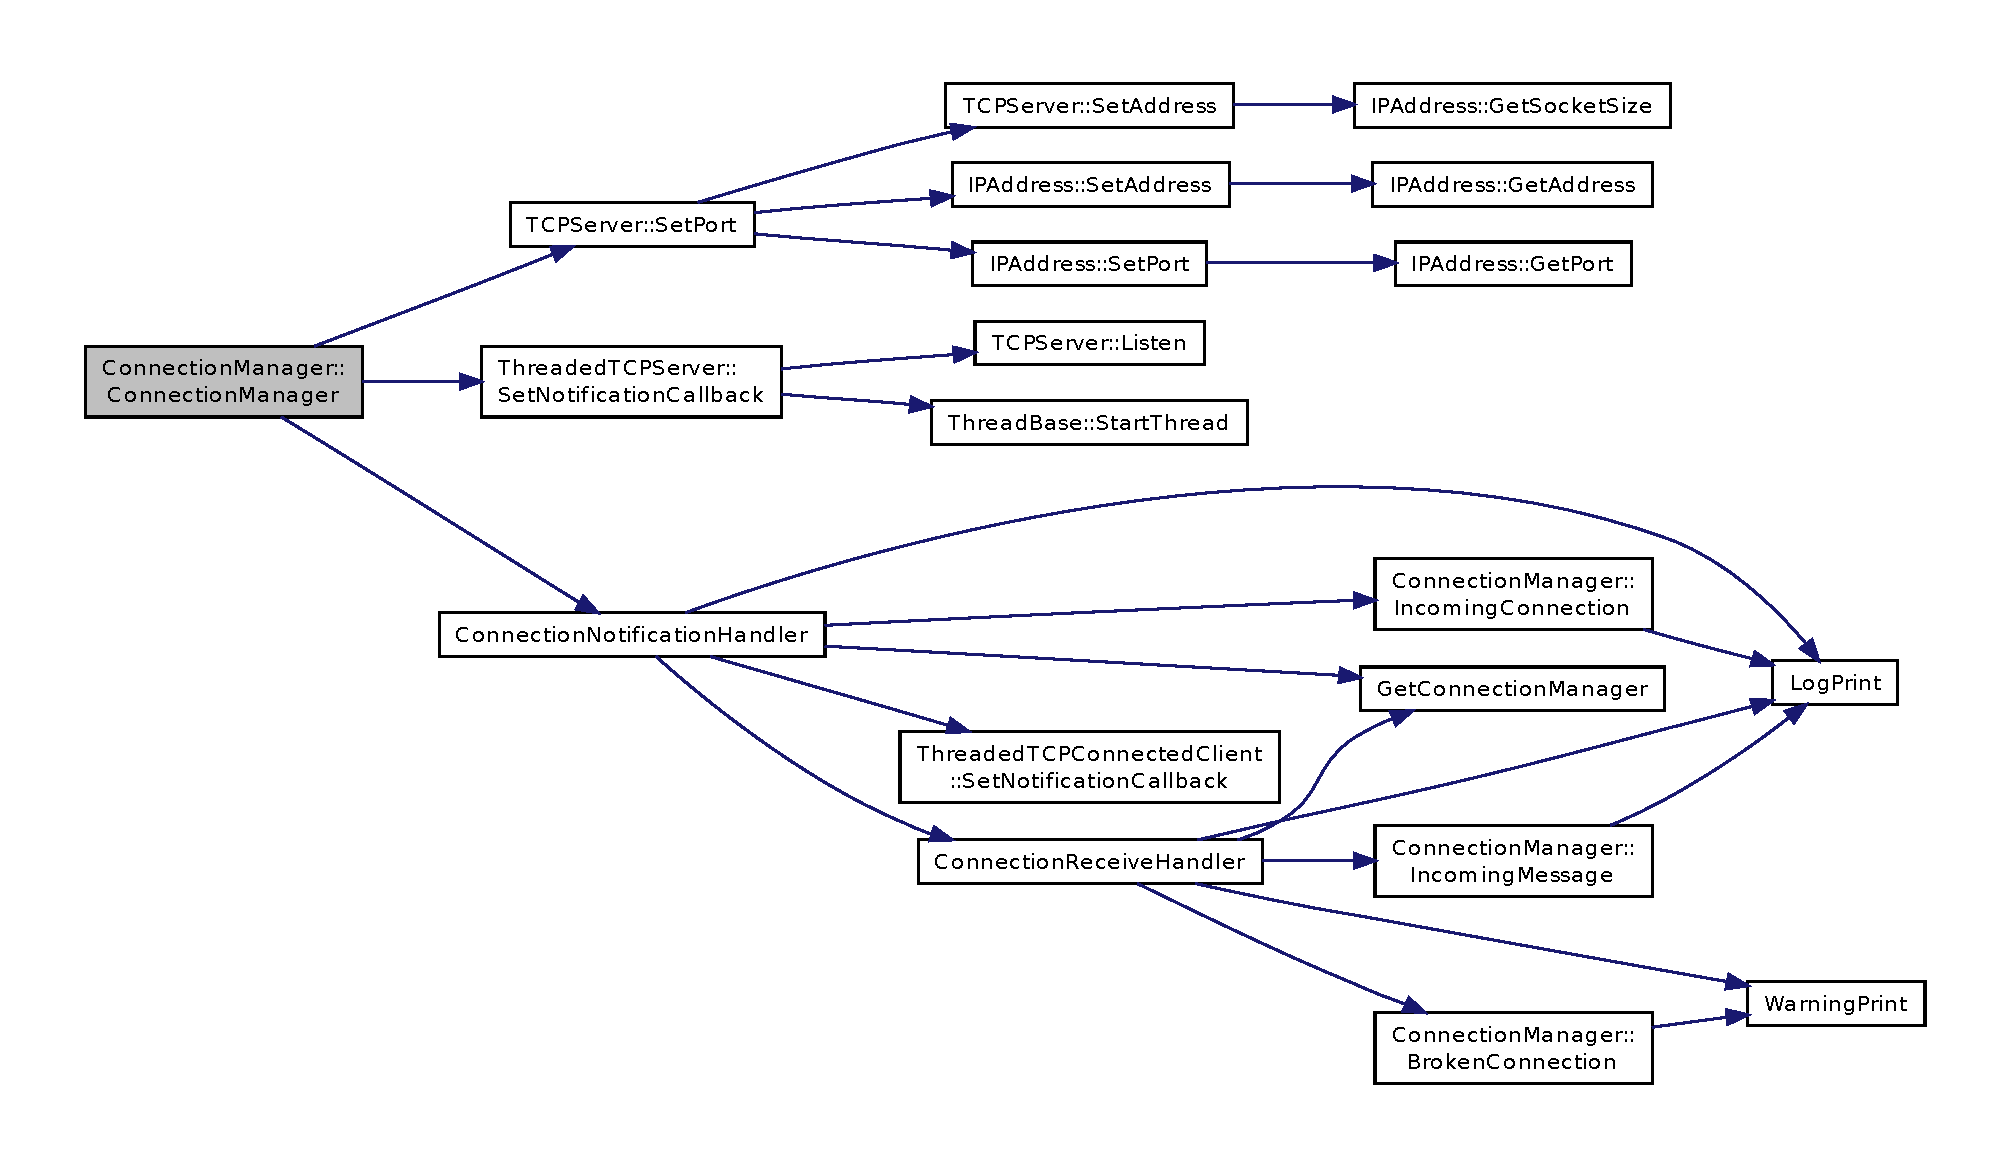
\includegraphics[width=350pt]{class_connection_manager_a7928f3e95b4e88b01c11eaf3e8089ee7_cgraph}
\end{center}
\end{figure}




\subsection{Member Function Documentation}
\hypertarget{class_connection_manager_a64473b0369ab91daf3a2da6b8ef576d0}{\index{Connection\-Manager@{Connection\-Manager}!Broken\-Connection@{Broken\-Connection}}
\index{Broken\-Connection@{Broken\-Connection}!ConnectionManager@{Connection\-Manager}}
\subsubsection[{Broken\-Connection}]{\setlength{\rightskip}{0pt plus 5cm}void Connection\-Manager\-::\-Broken\-Connection (
\begin{DoxyParamCaption}
\item[{{\bf Threaded\-T\-C\-P\-Connected\-Client} $\ast$}]{broken\-Client}
\end{DoxyParamCaption}
)}}\label{class_connection_manager_a64473b0369ab91daf3a2da6b8ef576d0}


Broken connection handler. 

This method handles a broken connection to an existing client. The \hyperlink{class_client_manager}{Client\-Manager} is notified, leaving the handling to it.


\begin{DoxyParams}{Parameters}
{\em broken\-Client} & T\-C\-P Information of the broken connection. \\
\hline
\end{DoxyParams}


Definition at line 66 of file Connection\-Manager.\-cpp.



Here is the call graph for this function\-:\nopagebreak
\begin{figure}[H]
\begin{center}
\leavevmode
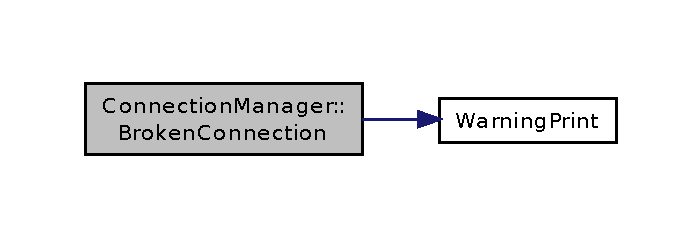
\includegraphics[width=336pt]{class_connection_manager_a64473b0369ab91daf3a2da6b8ef576d0_cgraph}
\end{center}
\end{figure}




Here is the caller graph for this function\-:\nopagebreak
\begin{figure}[H]
\begin{center}
\leavevmode
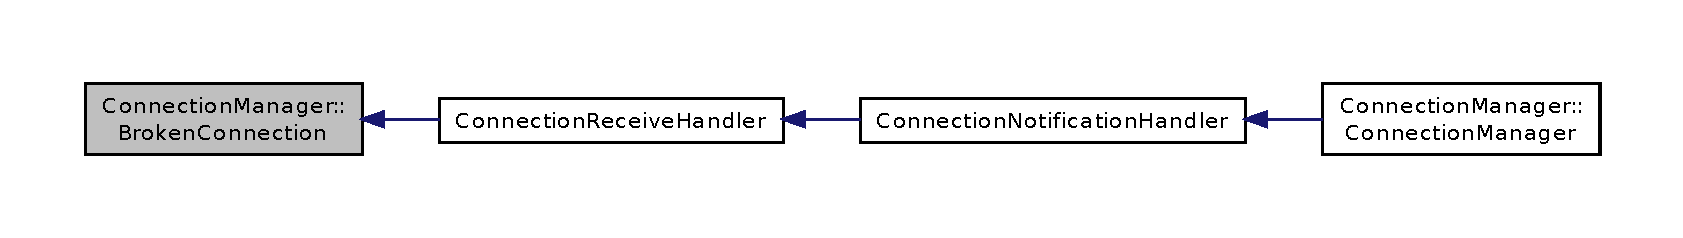
\includegraphics[width=350pt]{class_connection_manager_a64473b0369ab91daf3a2da6b8ef576d0_icgraph}
\end{center}
\end{figure}


\hypertarget{class_connection_manager_afc67553cf1eff6ab251a5dd2a313e863}{\index{Connection\-Manager@{Connection\-Manager}!Delete\-Client@{Delete\-Client}}
\index{Delete\-Client@{Delete\-Client}!ConnectionManager@{Connection\-Manager}}
\subsubsection[{Delete\-Client}]{\setlength{\rightskip}{0pt plus 5cm}void Connection\-Manager\-::\-Delete\-Client (
\begin{DoxyParamCaption}
\item[{{\bf Client\-Manager} $\ast$}]{client\-Manager}
\end{DoxyParamCaption}
)}}\label{class_connection_manager_afc67553cf1eff6ab251a5dd2a313e863}


Deletes the \hyperlink{class_client_manager}{Client\-Manager} from all lists and finally deletes itself. 


\begin{DoxyParams}{Parameters}
{\em client\-Manager} & \hyperlink{class_client_manager}{Client\-Manager} to be deleted. \\
\hline
\end{DoxyParams}


Definition at line 84 of file Connection\-Manager.\-cpp.



Here is the call graph for this function\-:\nopagebreak
\begin{figure}[H]
\begin{center}
\leavevmode
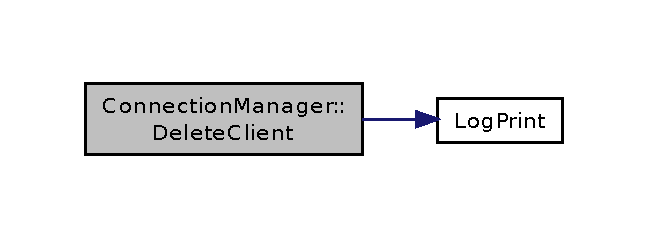
\includegraphics[width=310pt]{class_connection_manager_afc67553cf1eff6ab251a5dd2a313e863_cgraph}
\end{center}
\end{figure}




Here is the caller graph for this function\-:\nopagebreak
\begin{figure}[H]
\begin{center}
\leavevmode
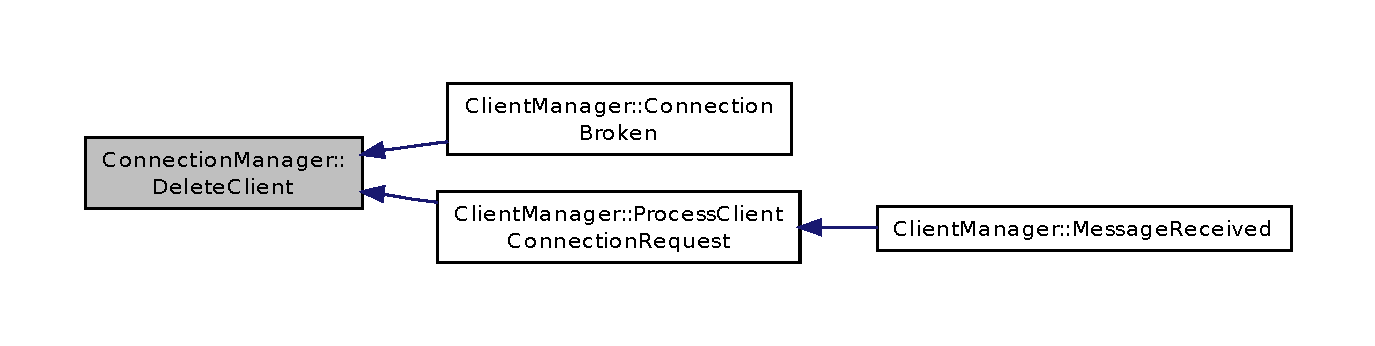
\includegraphics[width=350pt]{class_connection_manager_afc67553cf1eff6ab251a5dd2a313e863_icgraph}
\end{center}
\end{figure}


\hypertarget{class_connection_manager_adf13721cde7ae4615aadbb5262f67274}{\index{Connection\-Manager@{Connection\-Manager}!Get\-Number\-Of\-Clients@{Get\-Number\-Of\-Clients}}
\index{Get\-Number\-Of\-Clients@{Get\-Number\-Of\-Clients}!ConnectionManager@{Connection\-Manager}}
\subsubsection[{Get\-Number\-Of\-Clients}]{\setlength{\rightskip}{0pt plus 5cm}{\bf T\-Number\-Of\-Clients} Connection\-Manager\-::\-Get\-Number\-Of\-Clients (
\begin{DoxyParamCaption}
\item[{void}]{}
\end{DoxyParamCaption}
) const\hspace{0.3cm}{\ttfamily [inline]}}}\label{class_connection_manager_adf13721cde7ae4615aadbb5262f67274}


Returns the current number of clients connected. 

\begin{DoxyReturn}{Returns}
Number of connected clients. 
\end{DoxyReturn}


Definition at line 154 of file Connection\-Manager.\-h.



Here is the caller graph for this function\-:\nopagebreak
\begin{figure}[H]
\begin{center}
\leavevmode
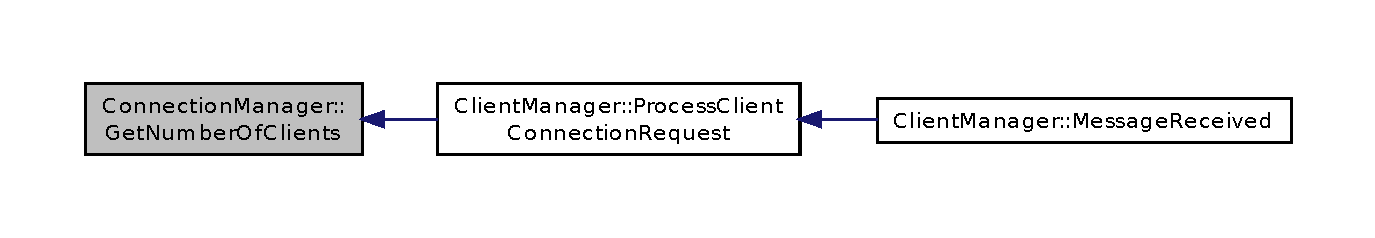
\includegraphics[width=350pt]{class_connection_manager_adf13721cde7ae4615aadbb5262f67274_icgraph}
\end{center}
\end{figure}


\hypertarget{class_connection_manager_a54968c1176475aa513538691b75aedc9}{\index{Connection\-Manager@{Connection\-Manager}!Incoming\-Connection@{Incoming\-Connection}}
\index{Incoming\-Connection@{Incoming\-Connection}!ConnectionManager@{Connection\-Manager}}
\subsubsection[{Incoming\-Connection}]{\setlength{\rightskip}{0pt plus 5cm}void Connection\-Manager\-::\-Incoming\-Connection (
\begin{DoxyParamCaption}
\item[{{\bf Threaded\-T\-C\-P\-Connected\-Client} $\ast$}]{new\-Client}
\end{DoxyParamCaption}
)}}\label{class_connection_manager_a54968c1176475aa513538691b75aedc9}


Incoming connection handler. 

This method handles a new connection from a new client. A new \hyperlink{class_client_manager}{Client\-Manager} is created and the information is added to the lists for book-\/keeping.


\begin{DoxyParams}{Parameters}
{\em new\-Client} & T\-C\-P Information of the new connection. \\
\hline
\end{DoxyParams}


Definition at line 54 of file Connection\-Manager.\-cpp.



Here is the call graph for this function\-:\nopagebreak
\begin{figure}[H]
\begin{center}
\leavevmode
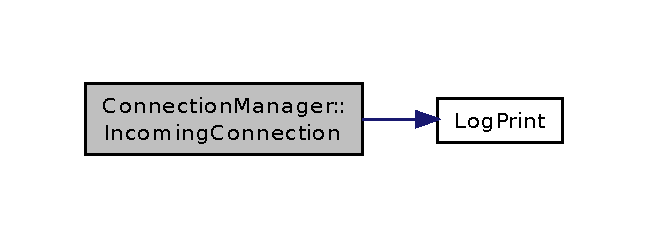
\includegraphics[width=310pt]{class_connection_manager_a54968c1176475aa513538691b75aedc9_cgraph}
\end{center}
\end{figure}




Here is the caller graph for this function\-:\nopagebreak
\begin{figure}[H]
\begin{center}
\leavevmode
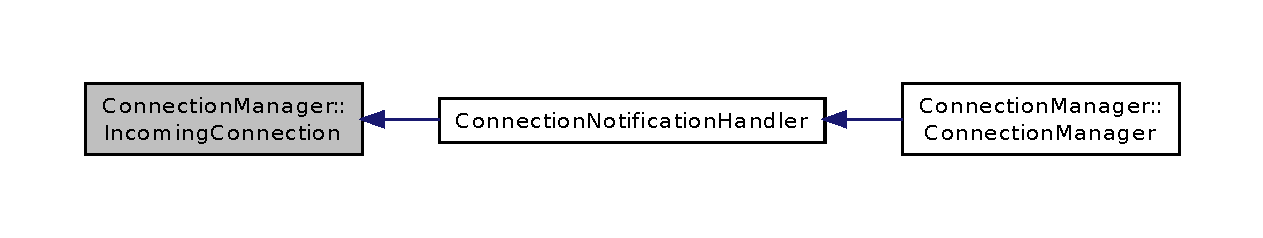
\includegraphics[width=350pt]{class_connection_manager_a54968c1176475aa513538691b75aedc9_icgraph}
\end{center}
\end{figure}


\hypertarget{class_connection_manager_a4657b51054ad28143f1bddd1f5cc282c}{\index{Connection\-Manager@{Connection\-Manager}!Incoming\-Message@{Incoming\-Message}}
\index{Incoming\-Message@{Incoming\-Message}!ConnectionManager@{Connection\-Manager}}
\subsubsection[{Incoming\-Message}]{\setlength{\rightskip}{0pt plus 5cm}void Connection\-Manager\-::\-Incoming\-Message (
\begin{DoxyParamCaption}
\item[{{\bf Threaded\-T\-C\-P\-Connected\-Client} $\ast$}]{sender\-Client, }
\item[{void $\ast$}]{buffer, }
\item[{size\-\_\-t}]{size}
\end{DoxyParamCaption}
)}}\label{class_connection_manager_a4657b51054ad28143f1bddd1f5cc282c}


New message processor. 

This method takes the received information and relays it to the respective \hyperlink{class_client_manager}{Client\-Manager}.


\begin{DoxyParams}{Parameters}
{\em sender\-Client} & T\-C\-P Information of the sender. \\
\hline
{\em buffer} & Buffer containing the received message. \\
\hline
{\em size} & Size of the received message. \\
\hline
\end{DoxyParams}


Definition at line 75 of file Connection\-Manager.\-cpp.



Here is the call graph for this function\-:\nopagebreak
\begin{figure}[H]
\begin{center}
\leavevmode
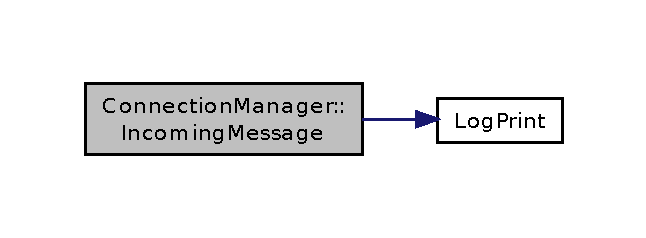
\includegraphics[width=310pt]{class_connection_manager_a4657b51054ad28143f1bddd1f5cc282c_cgraph}
\end{center}
\end{figure}




Here is the caller graph for this function\-:\nopagebreak
\begin{figure}[H]
\begin{center}
\leavevmode
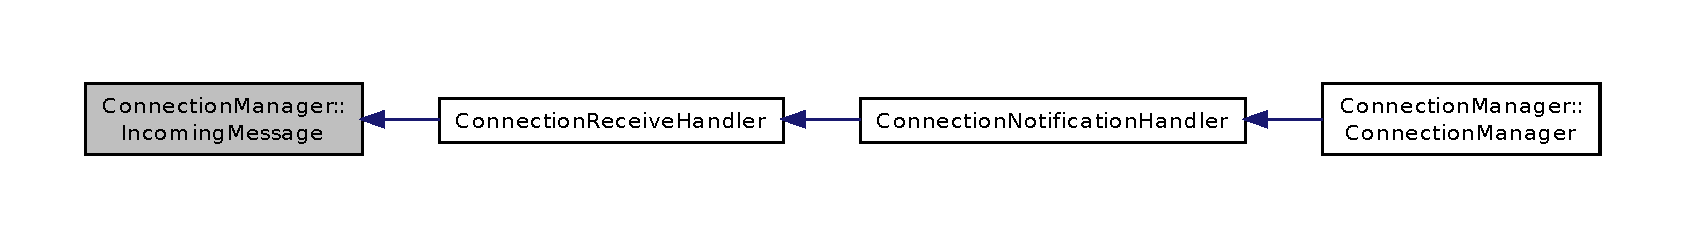
\includegraphics[width=350pt]{class_connection_manager_a4657b51054ad28143f1bddd1f5cc282c_icgraph}
\end{center}
\end{figure}




\subsection{Friends And Related Function Documentation}
\hypertarget{class_connection_manager_ab88124ce7a3bf1d2892d0e9763d1af30}{\index{Connection\-Manager@{Connection\-Manager}!Get\-Connection\-Manager@{Get\-Connection\-Manager}}
\index{Get\-Connection\-Manager@{Get\-Connection\-Manager}!ConnectionManager@{Connection\-Manager}}
\subsubsection[{Get\-Connection\-Manager}]{\setlength{\rightskip}{0pt plus 5cm}{\bf Connection\-Manager}\& Get\-Connection\-Manager (
\begin{DoxyParamCaption}
\item[{void}]{}
\end{DoxyParamCaption}
)\hspace{0.3cm}{\ttfamily [friend]}}}\label{class_connection_manager_ab88124ce7a3bf1d2892d0e9763d1af30}


Friend method for singleton implementation. 

\begin{DoxyReturn}{Returns}
Returns the reference to the \hyperlink{class_connection_manager}{Connection\-Manager}. 
\end{DoxyReturn}


Definition at line 11 of file Connection\-Manager.\-cpp.



\subsection{Member Data Documentation}
\hypertarget{class_connection_manager_ad9da7334bc0a1ed0f152f5998b46268a}{\index{Connection\-Manager@{Connection\-Manager}!m\-\_\-client\-List@{m\-\_\-client\-List}}
\index{m\-\_\-client\-List@{m\-\_\-client\-List}!ConnectionManager@{Connection\-Manager}}
\subsubsection[{m\-\_\-client\-List}]{\setlength{\rightskip}{0pt plus 5cm}{\bf T\-Client\-List} Connection\-Manager\-::m\-\_\-client\-List\hspace{0.3cm}{\ttfamily [private]}}}\label{class_connection_manager_ad9da7334bc0a1ed0f152f5998b46268a}


Holds the Connection-\/$>$Manager based list. 



Definition at line 89 of file Connection\-Manager.\-h.

\hypertarget{class_connection_manager_aae27a14334d4b84076231534196e75eb}{\index{Connection\-Manager@{Connection\-Manager}!m\-\_\-reversed\-Client\-List@{m\-\_\-reversed\-Client\-List}}
\index{m\-\_\-reversed\-Client\-List@{m\-\_\-reversed\-Client\-List}!ConnectionManager@{Connection\-Manager}}
\subsubsection[{m\-\_\-reversed\-Client\-List}]{\setlength{\rightskip}{0pt plus 5cm}{\bf T\-Reversed\-Client\-List} Connection\-Manager\-::m\-\_\-reversed\-Client\-List\hspace{0.3cm}{\ttfamily [private]}}}\label{class_connection_manager_aae27a14334d4b84076231534196e75eb}


Holds the Manager-\/$>$Connection based list for speed. 



Definition at line 94 of file Connection\-Manager.\-h.

\hypertarget{class_connection_manager_a8858415ddb04364d4697f7ea00aa2977}{\index{Connection\-Manager@{Connection\-Manager}!m\-\_\-server@{m\-\_\-server}}
\index{m\-\_\-server@{m\-\_\-server}!ConnectionManager@{Connection\-Manager}}
\subsubsection[{m\-\_\-server}]{\setlength{\rightskip}{0pt plus 5cm}{\bf Threaded\-T\-C\-P\-Server} Connection\-Manager\-::m\-\_\-server\hspace{0.3cm}{\ttfamily [private]}}}\label{class_connection_manager_a8858415ddb04364d4697f7ea00aa2977}


Instance of the T\-C\-P server. 



Definition at line 99 of file Connection\-Manager.\-h.



The documentation for this class was generated from the following files\-:\begin{DoxyCompactItemize}
\item 
S2\-Sim/\hyperlink{_connection_manager_8h}{Connection\-Manager.\-h}\item 
S2\-Sim/\hyperlink{_connection_manager_8cpp}{Connection\-Manager.\-cpp}\end{DoxyCompactItemize}

\hypertarget{class_control_manager}{\section{Control\-Manager Class Reference}
\label{class_control_manager}\index{Control\-Manager@{Control\-Manager}}
}


Manager the connection with the External Controller.  




{\ttfamily \#include $<$Control\-Manager.\-h$>$}



Collaboration diagram for Control\-Manager\-:\nopagebreak
\begin{figure}[H]
\begin{center}
\leavevmode
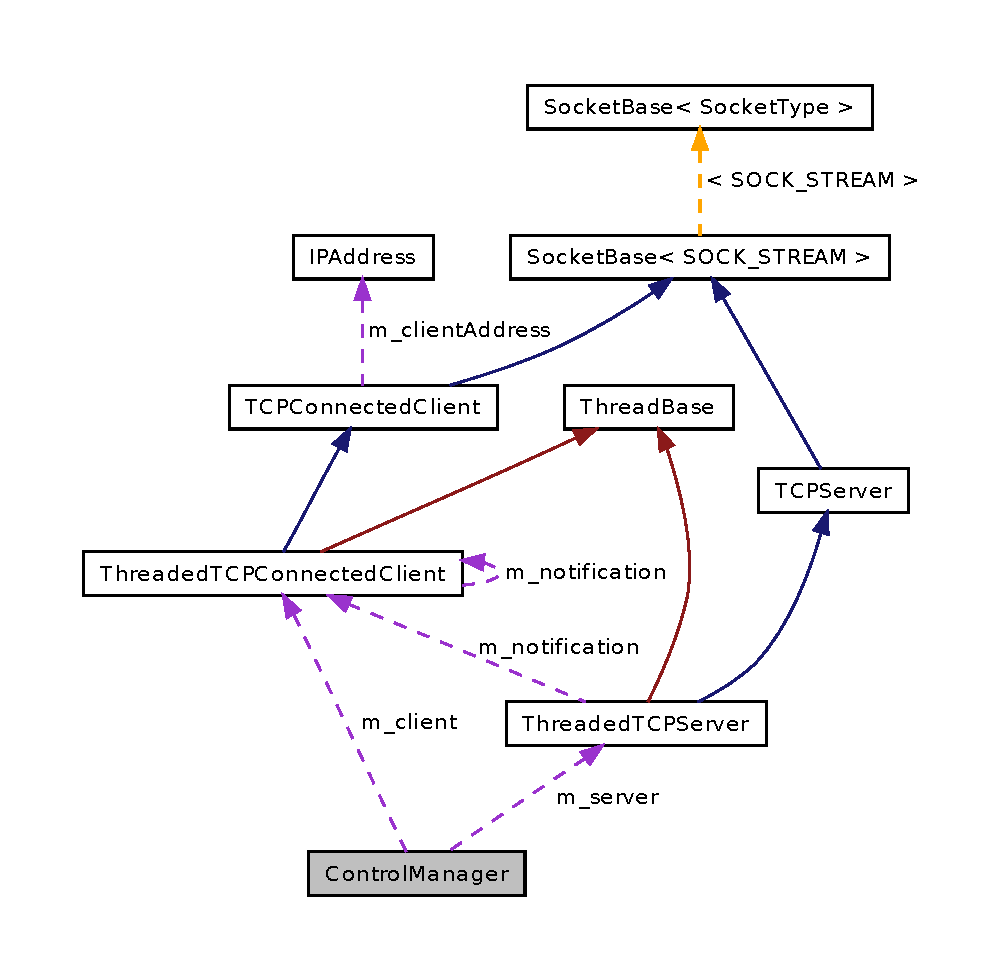
\includegraphics[width=350pt]{class_control_manager__coll__graph}
\end{center}
\end{figure}
\subsection*{Public Types}
\begin{DoxyCompactItemize}
\item 
typedef \\*
\hyperlink{class_terra_swarm_1_1_asynchronous_1_1_client_data_ac733720fed15e940f991de44f1bb514e}{Asynchronous\-::\-Client\-Data\-::\-T\-Data\-Point} \hyperlink{class_control_manager_a336440023399b9165c117020f6b14ec3}{T\-Voltage}
\item 
typedef \\*
\hyperlink{class_terra_swarm_1_1_asynchronous_1_1_client_data_ac733720fed15e940f991de44f1bb514e}{Asynchronous\-::\-Client\-Data\-::\-T\-Data\-Point} \hyperlink{class_control_manager_a24609feed8b0443df450b070194df20a}{T\-Wattage}
\item 
typedef \hyperlink{class_terra_swarm_1_1_message_header_ab55de822fadad758edcd8f36bd07676e}{Message\-Header\-::\-T\-Id} \hyperlink{class_control_manager_a7eefb0a4e9d10e65771939912d650bcc}{T\-Number\-Of\-Clients}
\item 
typedef \hyperlink{class_terra_swarm_1_1_message_header_ab55de822fadad758edcd8f36bd07676e}{Message\-Header\-::\-T\-Id} \hyperlink{class_control_manager_a1bff13cab35db39c43f81f49b56e4849}{T\-Client\-Id}
\item 
typedef \\*
\hyperlink{class_terra_swarm_1_1_asynchronous_1_1_client_connection_request_a50a16fcfef8eb10d5191b6eaf0723a92}{Asynchronous\-::\-Client\-Connection\-Request\-::\-T\-Client\-Name} \hyperlink{class_control_manager_ae9c86c5286c9ebf222ea44b60c463872}{T\-Client\-Name}
\item 
typedef \\*
\hyperlink{class_terra_swarm_1_1_asynchronous_1_1_client_data_ac733720fed15e940f991de44f1bb514e}{Asynchronous\-::\-Client\-Data\-::\-T\-Data\-Point} \hyperlink{class_control_manager_acad2d80fd0659e3d979389de905e7b5b}{T\-Price}
\item 
typedef \\*
\hyperlink{class_terra_swarm_1_1_asynchronous_1_1_client_data_ac733720fed15e940f991de44f1bb514e}{Asynchronous\-::\-Client\-Data\-::\-T\-Data\-Point} \hyperlink{class_control_manager_a236ef5279ad4f3082443e4c6d300a7d2}{T\-Data\-Point}
\item 
typedef \\*
\hyperlink{class_terra_swarm_1_1_asynchronous_1_1_client_data_a690994afd0ba9b8eeb56ae679a5c64e8}{Asynchronous\-::\-Client\-Data\-::\-T\-Number\-Of\-Data\-Points} \hyperlink{class_control_manager_a90ca5d46699df9c6e67c96e36727eff1}{T\-Number\-Of\-Data\-Points}
\end{DoxyCompactItemize}
\subsection*{Public Member Functions}
\begin{DoxyCompactItemize}
\item 
void \hyperlink{class_control_manager_a67d548535b36a78e315a0aa5f9f8e6c8}{Set\-Client} (\hyperlink{class_threaded_t_c_p_connected_client}{Threaded\-T\-C\-P\-Connected\-Client} $\ast$client)
\item 
void \hyperlink{class_control_manager_a2dc55da1b01fd175b3d885c68b8a7524}{Process\-Data} (void $\ast$data, const size\-\_\-t size)
\begin{DoxyCompactList}\small\item\em Processes the received message from the External Controller. \end{DoxyCompactList}\item 
void \hyperlink{class_control_manager_a0d5212df17307aef87d42add3aa6cc7a}{Make\-Decision} (void)
\begin{DoxyCompactList}\small\item\em Starts the decision process by sending necessary information to External Controller. \end{DoxyCompactList}\item 
void \hyperlink{class_control_manager_a4e23ffb481554c26cf99c411dd16ae36}{Wait\-Until\-Ready} (void)
\item 
void \hyperlink{class_control_manager_a56df538a5380c9091123a5a8a5e0fe86}{Register\-Client} (const \hyperlink{class_control_manager_a1bff13cab35db39c43f81f49b56e4849}{T\-Client\-Id} client\-Id, const \hyperlink{class_control_manager_ae9c86c5286c9ebf222ea44b60c463872}{T\-Client\-Name} \&client\-Name, \hyperlink{class_client_manager}{Client\-Manager} $\ast$client\-Manager)
\item 
void \hyperlink{class_control_manager_ac3c913a01fe2e5e5467ad3d140c8e9a2}{Un\-Register\-Client} (const \hyperlink{class_control_manager_a1bff13cab35db39c43f81f49b56e4849}{T\-Client\-Id} client\-Id)
\item 
void \hyperlink{class_control_manager_aa4398a05586d9b711aa6101334deefe1}{Client\-Price\-Request} (const \hyperlink{class_control_manager_a1bff13cab35db39c43f81f49b56e4849}{T\-Client\-Id} client\-Id)
\item 
void \hyperlink{class_control_manager_a5b551f560431d0bb0bcf6c338bac8eb3}{Client\-Demand\-Negotiation} (const \hyperlink{class_control_manager_a1bff13cab35db39c43f81f49b56e4849}{T\-Client\-Id} client\-Id, const \hyperlink{class_control_manager_a90ca5d46699df9c6e67c96e36727eff1}{T\-Number\-Of\-Data\-Points} number\-Of\-Data\-Points, \hyperlink{class_control_manager_a236ef5279ad4f3082443e4c6d300a7d2}{T\-Data\-Point} $\ast$data\-Points)
\item 
\hyperlink{class_control_manager_ae9c86c5286c9ebf222ea44b60c463872}{T\-Client\-Name} \hyperlink{class_control_manager_a927449c3a4ba8a5bdc23e3747d5bb077}{Get\-Client\-Name} (const \hyperlink{class_control_manager_a1bff13cab35db39c43f81f49b56e4849}{T\-Client\-Id} client\-Id)
\end{DoxyCompactItemize}
\subsection*{Private Types}
\begin{DoxyCompactItemize}
\item 
enum \hyperlink{class_control_manager_a7b6de4a130e0de1729c7963edd972120}{Message\-Type\-Values} \{ \\*
\hyperlink{class_control_manager_a7b6de4a130e0de1729c7963edd972120afe62fd2d680bfeddc030a63944f8e513}{Make\-Decision\-Type} = 0x00000001, 
\hyperlink{class_control_manager_a7b6de4a130e0de1729c7963edd972120ae327aef118d20067ec6968987e76580d}{Decision\-Finished\-Type} = 0x00000002, 
\hyperlink{class_control_manager_a7b6de4a130e0de1729c7963edd972120ad0a806bbe260a48560eeeda4ffd855d6}{Set\-Price\-Type} = 0x00000003, 
\hyperlink{class_control_manager_a7b6de4a130e0de1729c7963edd972120ad493a309cdd6a23cc9e78a2e17eaf47d}{Send\-Price\-Proposal\-Type} = 0x00000004, 
\\*
\hyperlink{class_control_manager_a7b6de4a130e0de1729c7963edd972120afad3b5e04ece26c7ec3a5f388db53b43}{Price\-Request\-Type} = 0x00000005, 
\hyperlink{class_control_manager_a7b6de4a130e0de1729c7963edd972120a8adf22182deb49ea93b62097e2618cff}{Demand\-Negotiation\-Type} = 0x00000006
 \}
\item 
typedef size\-\_\-t \hyperlink{class_control_manager_a5c898e9e00806858a59700370560aea7}{T\-Data\-Size}
\item 
typedef unsigned int \hyperlink{class_control_manager_a36b60e90749624a648dc225c2c136397}{T\-Message\-Type}
\item 
typedef std\-::map$<$ \hyperlink{class_control_manager_a1bff13cab35db39c43f81f49b56e4849}{T\-Client\-Id}, \\*
\hyperlink{class_control_manager_ae9c86c5286c9ebf222ea44b60c463872}{T\-Client\-Name} $>$ \hyperlink{class_control_manager_a5f6aa6ca619f6aa8dddfc3d5000162f0}{T\-Client\-Id\-Map}
\item 
typedef std\-::map$<$ \hyperlink{class_control_manager_a1bff13cab35db39c43f81f49b56e4849}{T\-Client\-Id}, \\*
\hyperlink{class_client_manager}{Client\-Manager} $\ast$ $>$ \hyperlink{class_control_manager_a27b18022695359e2a4d5563f91b6befd}{T\-Client\-Manager\-Map}
\end{DoxyCompactItemize}
\subsection*{Private Member Functions}
\begin{DoxyCompactItemize}
\item 
\hyperlink{class_control_manager_ab81bac3e592705b7ca4b23ce473fe26e}{Control\-Manager} (void)
\end{DoxyCompactItemize}
\subsection*{Private Attributes}
\begin{DoxyCompactItemize}
\item 
\hyperlink{class_threaded_t_c_p_server}{Threaded\-T\-C\-P\-Server} \hyperlink{class_control_manager_a1b71eabaeddfd8ec80e503b734c72e9d}{m\-\_\-server}
\item 
\hyperlink{class_threaded_t_c_p_connected_client}{Threaded\-T\-C\-P\-Connected\-Client} $\ast$ \hyperlink{class_control_manager_a3081c331c70f5b08dc0ef2615d86cc55}{m\-\_\-client}
\item 
Semaphore \hyperlink{class_control_manager_ab718d2d17750dfea91411de871855075}{m\-\_\-ready\-Semaphore}
\item 
\hyperlink{class_control_manager_a5f6aa6ca619f6aa8dddfc3d5000162f0}{T\-Client\-Id\-Map} \hyperlink{class_control_manager_a5623f6ef4da21d143a7a6cf5fbee136f}{m\-\_\-client\-Id\-Map}
\item 
\hyperlink{class_control_manager_a27b18022695359e2a4d5563f91b6befd}{T\-Client\-Manager\-Map} \hyperlink{class_control_manager_af47dee5a077190c6aeb7b9ef3d9cfb3b}{m\-\_\-client\-Manager\-Map}
\end{DoxyCompactItemize}
\subsection*{Friends}
\begin{DoxyCompactItemize}
\item 
\hyperlink{class_control_manager}{Control\-Manager} \& \hyperlink{class_control_manager_a63bfd4667c9c70297f25ae5e5176818e}{Get\-Control\-Manager} (void)
\begin{DoxyCompactList}\small\item\em Returns the only instance of \hyperlink{class_control_manager}{Control\-Manager}. \end{DoxyCompactList}\end{DoxyCompactItemize}


\subsection{Detailed Description}
Manager the connection with the External Controller. 

This class manages the connection to the External Controller. All received commands are processed and necessary updates are sent back. 

Definition at line 63 of file Control\-Manager.\-h.



\subsection{Member Typedef Documentation}
\hypertarget{class_control_manager_a1bff13cab35db39c43f81f49b56e4849}{\index{Control\-Manager@{Control\-Manager}!T\-Client\-Id@{T\-Client\-Id}}
\index{T\-Client\-Id@{T\-Client\-Id}!ControlManager@{Control\-Manager}}
\subsubsection[{T\-Client\-Id}]{\setlength{\rightskip}{0pt plus 5cm}typedef {\bf Message\-Header\-::\-T\-Id} {\bf Control\-Manager\-::\-T\-Client\-Id}}}\label{class_control_manager_a1bff13cab35db39c43f81f49b56e4849}
Redefines the type for unique id for rapid development. 

Definition at line 92 of file Control\-Manager.\-h.

\hypertarget{class_control_manager_a5f6aa6ca619f6aa8dddfc3d5000162f0}{\index{Control\-Manager@{Control\-Manager}!T\-Client\-Id\-Map@{T\-Client\-Id\-Map}}
\index{T\-Client\-Id\-Map@{T\-Client\-Id\-Map}!ControlManager@{Control\-Manager}}
\subsubsection[{T\-Client\-Id\-Map}]{\setlength{\rightskip}{0pt plus 5cm}typedef std\-::map$<${\bf T\-Client\-Id}, {\bf T\-Client\-Name}$>$ {\bf Control\-Manager\-::\-T\-Client\-Id\-Map}\hspace{0.3cm}{\ttfamily [private]}}}\label{class_control_manager_a5f6aa6ca619f6aa8dddfc3d5000162f0}
Defines the type holding a Client\-Id-\/$>$Client\-Name mapping. 

Definition at line 141 of file Control\-Manager.\-h.

\hypertarget{class_control_manager_a27b18022695359e2a4d5563f91b6befd}{\index{Control\-Manager@{Control\-Manager}!T\-Client\-Manager\-Map@{T\-Client\-Manager\-Map}}
\index{T\-Client\-Manager\-Map@{T\-Client\-Manager\-Map}!ControlManager@{Control\-Manager}}
\subsubsection[{T\-Client\-Manager\-Map}]{\setlength{\rightskip}{0pt plus 5cm}typedef std\-::map$<${\bf T\-Client\-Id},{\bf Client\-Manager}$\ast$$>$ {\bf Control\-Manager\-::\-T\-Client\-Manager\-Map}\hspace{0.3cm}{\ttfamily [private]}}}\label{class_control_manager_a27b18022695359e2a4d5563f91b6befd}
Defines the type holding a Client\-Id-\/$>$\hyperlink{class_client_manager}{Client\-Manager} mapping. 

Definition at line 146 of file Control\-Manager.\-h.

\hypertarget{class_control_manager_ae9c86c5286c9ebf222ea44b60c463872}{\index{Control\-Manager@{Control\-Manager}!T\-Client\-Name@{T\-Client\-Name}}
\index{T\-Client\-Name@{T\-Client\-Name}!ControlManager@{Control\-Manager}}
\subsubsection[{T\-Client\-Name}]{\setlength{\rightskip}{0pt plus 5cm}typedef {\bf Asynchronous\-::\-Client\-Connection\-Request\-::\-T\-Client\-Name} {\bf Control\-Manager\-::\-T\-Client\-Name}}}\label{class_control_manager_ae9c86c5286c9ebf222ea44b60c463872}
Redefines the type for object name for rapid development. 

Definition at line 97 of file Control\-Manager.\-h.

\hypertarget{class_control_manager_a236ef5279ad4f3082443e4c6d300a7d2}{\index{Control\-Manager@{Control\-Manager}!T\-Data\-Point@{T\-Data\-Point}}
\index{T\-Data\-Point@{T\-Data\-Point}!ControlManager@{Control\-Manager}}
\subsubsection[{T\-Data\-Point}]{\setlength{\rightskip}{0pt plus 5cm}typedef {\bf Asynchronous\-::\-Client\-Data\-::\-T\-Data\-Point} {\bf Control\-Manager\-::\-T\-Data\-Point}}}\label{class_control_manager_a236ef5279ad4f3082443e4c6d300a7d2}
Redefines the general data type for rapid development. 

Definition at line 107 of file Control\-Manager.\-h.

\hypertarget{class_control_manager_a5c898e9e00806858a59700370560aea7}{\index{Control\-Manager@{Control\-Manager}!T\-Data\-Size@{T\-Data\-Size}}
\index{T\-Data\-Size@{T\-Data\-Size}!ControlManager@{Control\-Manager}}
\subsubsection[{T\-Data\-Size}]{\setlength{\rightskip}{0pt plus 5cm}typedef size\-\_\-t {\bf Control\-Manager\-::\-T\-Data\-Size}\hspace{0.3cm}{\ttfamily [private]}}}\label{class_control_manager_a5c898e9e00806858a59700370560aea7}
Defines the type for size of a data chunk. 

Definition at line 118 of file Control\-Manager.\-h.

\hypertarget{class_control_manager_a36b60e90749624a648dc225c2c136397}{\index{Control\-Manager@{Control\-Manager}!T\-Message\-Type@{T\-Message\-Type}}
\index{T\-Message\-Type@{T\-Message\-Type}!ControlManager@{Control\-Manager}}
\subsubsection[{T\-Message\-Type}]{\setlength{\rightskip}{0pt plus 5cm}typedef unsigned int {\bf Control\-Manager\-::\-T\-Message\-Type}\hspace{0.3cm}{\ttfamily [private]}}}\label{class_control_manager_a36b60e90749624a648dc225c2c136397}
Defines the message type field used in the communication for message processing. 

Definition at line 123 of file Control\-Manager.\-h.

\hypertarget{class_control_manager_a7eefb0a4e9d10e65771939912d650bcc}{\index{Control\-Manager@{Control\-Manager}!T\-Number\-Of\-Clients@{T\-Number\-Of\-Clients}}
\index{T\-Number\-Of\-Clients@{T\-Number\-Of\-Clients}!ControlManager@{Control\-Manager}}
\subsubsection[{T\-Number\-Of\-Clients}]{\setlength{\rightskip}{0pt plus 5cm}typedef {\bf Message\-Header\-::\-T\-Id} {\bf Control\-Manager\-::\-T\-Number\-Of\-Clients}}}\label{class_control_manager_a7eefb0a4e9d10e65771939912d650bcc}
Defines the type of number of clients. 

Definition at line 87 of file Control\-Manager.\-h.

\hypertarget{class_control_manager_a90ca5d46699df9c6e67c96e36727eff1}{\index{Control\-Manager@{Control\-Manager}!T\-Number\-Of\-Data\-Points@{T\-Number\-Of\-Data\-Points}}
\index{T\-Number\-Of\-Data\-Points@{T\-Number\-Of\-Data\-Points}!ControlManager@{Control\-Manager}}
\subsubsection[{T\-Number\-Of\-Data\-Points}]{\setlength{\rightskip}{0pt plus 5cm}typedef {\bf Asynchronous\-::\-Client\-Data\-::\-T\-Number\-Of\-Data\-Points} {\bf Control\-Manager\-::\-T\-Number\-Of\-Data\-Points}}}\label{class_control_manager_a90ca5d46699df9c6e67c96e36727eff1}
Redefines the number of data points type for rapid development. 

Definition at line 112 of file Control\-Manager.\-h.

\hypertarget{class_control_manager_acad2d80fd0659e3d979389de905e7b5b}{\index{Control\-Manager@{Control\-Manager}!T\-Price@{T\-Price}}
\index{T\-Price@{T\-Price}!ControlManager@{Control\-Manager}}
\subsubsection[{T\-Price}]{\setlength{\rightskip}{0pt plus 5cm}typedef {\bf Asynchronous\-::\-Client\-Data\-::\-T\-Data\-Point} {\bf Control\-Manager\-::\-T\-Price}}}\label{class_control_manager_acad2d80fd0659e3d979389de905e7b5b}
Defines the type for the price feedback signal. 

Definition at line 102 of file Control\-Manager.\-h.

\hypertarget{class_control_manager_a336440023399b9165c117020f6b14ec3}{\index{Control\-Manager@{Control\-Manager}!T\-Voltage@{T\-Voltage}}
\index{T\-Voltage@{T\-Voltage}!ControlManager@{Control\-Manager}}
\subsubsection[{T\-Voltage}]{\setlength{\rightskip}{0pt plus 5cm}typedef {\bf Asynchronous\-::\-Client\-Data\-::\-T\-Data\-Point} {\bf Control\-Manager\-::\-T\-Voltage}}}\label{class_control_manager_a336440023399b9165c117020f6b14ec3}
Defines the type of Voltage information. 

Definition at line 77 of file Control\-Manager.\-h.

\hypertarget{class_control_manager_a24609feed8b0443df450b070194df20a}{\index{Control\-Manager@{Control\-Manager}!T\-Wattage@{T\-Wattage}}
\index{T\-Wattage@{T\-Wattage}!ControlManager@{Control\-Manager}}
\subsubsection[{T\-Wattage}]{\setlength{\rightskip}{0pt plus 5cm}typedef {\bf Asynchronous\-::\-Client\-Data\-::\-T\-Data\-Point} {\bf Control\-Manager\-::\-T\-Wattage}}}\label{class_control_manager_a24609feed8b0443df450b070194df20a}
Defines the type of Wattage/\-Power information. 

Definition at line 82 of file Control\-Manager.\-h.



\subsection{Member Enumeration Documentation}
\hypertarget{class_control_manager_a7b6de4a130e0de1729c7963edd972120}{\index{Control\-Manager@{Control\-Manager}!Message\-Type\-Values@{Message\-Type\-Values}}
\index{Message\-Type\-Values@{Message\-Type\-Values}!ControlManager@{Control\-Manager}}
\subsubsection[{Message\-Type\-Values}]{\setlength{\rightskip}{0pt plus 5cm}enum {\bf Control\-Manager\-::\-Message\-Type\-Values}\hspace{0.3cm}{\ttfamily [private]}}}\label{class_control_manager_a7b6de4a130e0de1729c7963edd972120}
Defines the available values for different message types. \begin{Desc}
\item[Enumerator]\par
\begin{description}
\index{Make\-Decision\-Type@{Make\-Decision\-Type}!Control\-Manager@{Control\-Manager}}\index{Control\-Manager@{Control\-Manager}!Make\-Decision\-Type@{Make\-Decision\-Type}}\item[{\em 
\hypertarget{class_control_manager_a7b6de4a130e0de1729c7963edd972120afe62fd2d680bfeddc030a63944f8e513}{Make\-Decision\-Type}\label{class_control_manager_a7b6de4a130e0de1729c7963edd972120afe62fd2d680bfeddc030a63944f8e513}
}]Sent to external controller to indicate the beginning of a frame. \index{Decision\-Finished\-Type@{Decision\-Finished\-Type}!Control\-Manager@{Control\-Manager}}\index{Control\-Manager@{Control\-Manager}!Decision\-Finished\-Type@{Decision\-Finished\-Type}}\item[{\em 
\hypertarget{class_control_manager_a7b6de4a130e0de1729c7963edd972120ae327aef118d20067ec6968987e76580d}{Decision\-Finished\-Type}\label{class_control_manager_a7b6de4a130e0de1729c7963edd972120ae327aef118d20067ec6968987e76580d}
}]Received from external controller for the end of a frame. \index{Set\-Price\-Type@{Set\-Price\-Type}!Control\-Manager@{Control\-Manager}}\index{Control\-Manager@{Control\-Manager}!Set\-Price\-Type@{Set\-Price\-Type}}\item[{\em 
\hypertarget{class_control_manager_a7b6de4a130e0de1729c7963edd972120ad0a806bbe260a48560eeeda4ffd855d6}{Set\-Price\-Type}\label{class_control_manager_a7b6de4a130e0de1729c7963edd972120ad0a806bbe260a48560eeeda4ffd855d6}
}]Sent by external controller to send a price signal to a client. \index{Send\-Price\-Proposal\-Type@{Send\-Price\-Proposal\-Type}!Control\-Manager@{Control\-Manager}}\index{Control\-Manager@{Control\-Manager}!Send\-Price\-Proposal\-Type@{Send\-Price\-Proposal\-Type}}\item[{\em 
\hypertarget{class_control_manager_a7b6de4a130e0de1729c7963edd972120ad493a309cdd6a23cc9e78a2e17eaf47d}{Send\-Price\-Proposal\-Type}\label{class_control_manager_a7b6de4a130e0de1729c7963edd972120ad493a309cdd6a23cc9e78a2e17eaf47d}
}]Sent by external controller to send a price proposal to a client. \index{Price\-Request\-Type@{Price\-Request\-Type}!Control\-Manager@{Control\-Manager}}\index{Control\-Manager@{Control\-Manager}!Price\-Request\-Type@{Price\-Request\-Type}}\item[{\em 
\hypertarget{class_control_manager_a7b6de4a130e0de1729c7963edd972120afad3b5e04ece26c7ec3a5f388db53b43}{Price\-Request\-Type}\label{class_control_manager_a7b6de4a130e0de1729c7963edd972120afad3b5e04ece26c7ec3a5f388db53b43}
}]Sent to external controller to indicate a price request by a client. \index{Demand\-Negotiation\-Type@{Demand\-Negotiation\-Type}!Control\-Manager@{Control\-Manager}}\index{Control\-Manager@{Control\-Manager}!Demand\-Negotiation\-Type@{Demand\-Negotiation\-Type}}\item[{\em 
\hypertarget{class_control_manager_a7b6de4a130e0de1729c7963edd972120a8adf22182deb49ea93b62097e2618cff}{Demand\-Negotiation\-Type}\label{class_control_manager_a7b6de4a130e0de1729c7963edd972120a8adf22182deb49ea93b62097e2618cff}
}]Sent to external controller to indicate a price proposal response by a client. \end{description}
\end{Desc}


Definition at line 128 of file Control\-Manager.\-h.



\subsection{Constructor \& Destructor Documentation}
\hypertarget{class_control_manager_ab81bac3e592705b7ca4b23ce473fe26e}{\index{Control\-Manager@{Control\-Manager}!Control\-Manager@{Control\-Manager}}
\index{Control\-Manager@{Control\-Manager}!ControlManager@{Control\-Manager}}
\subsubsection[{Control\-Manager}]{\setlength{\rightskip}{0pt plus 5cm}Control\-Manager\-::\-Control\-Manager (
\begin{DoxyParamCaption}
\item[{void}]{}
\end{DoxyParamCaption}
)\hspace{0.3cm}{\ttfamily [private]}}}\label{class_control_manager_ab81bac3e592705b7ca4b23ce473fe26e}
Private constructor for singleton implementation. 

Definition at line 35 of file Control\-Manager.\-cpp.



Here is the call graph for this function\-:
\nopagebreak
\begin{figure}[H]
\begin{center}
\leavevmode
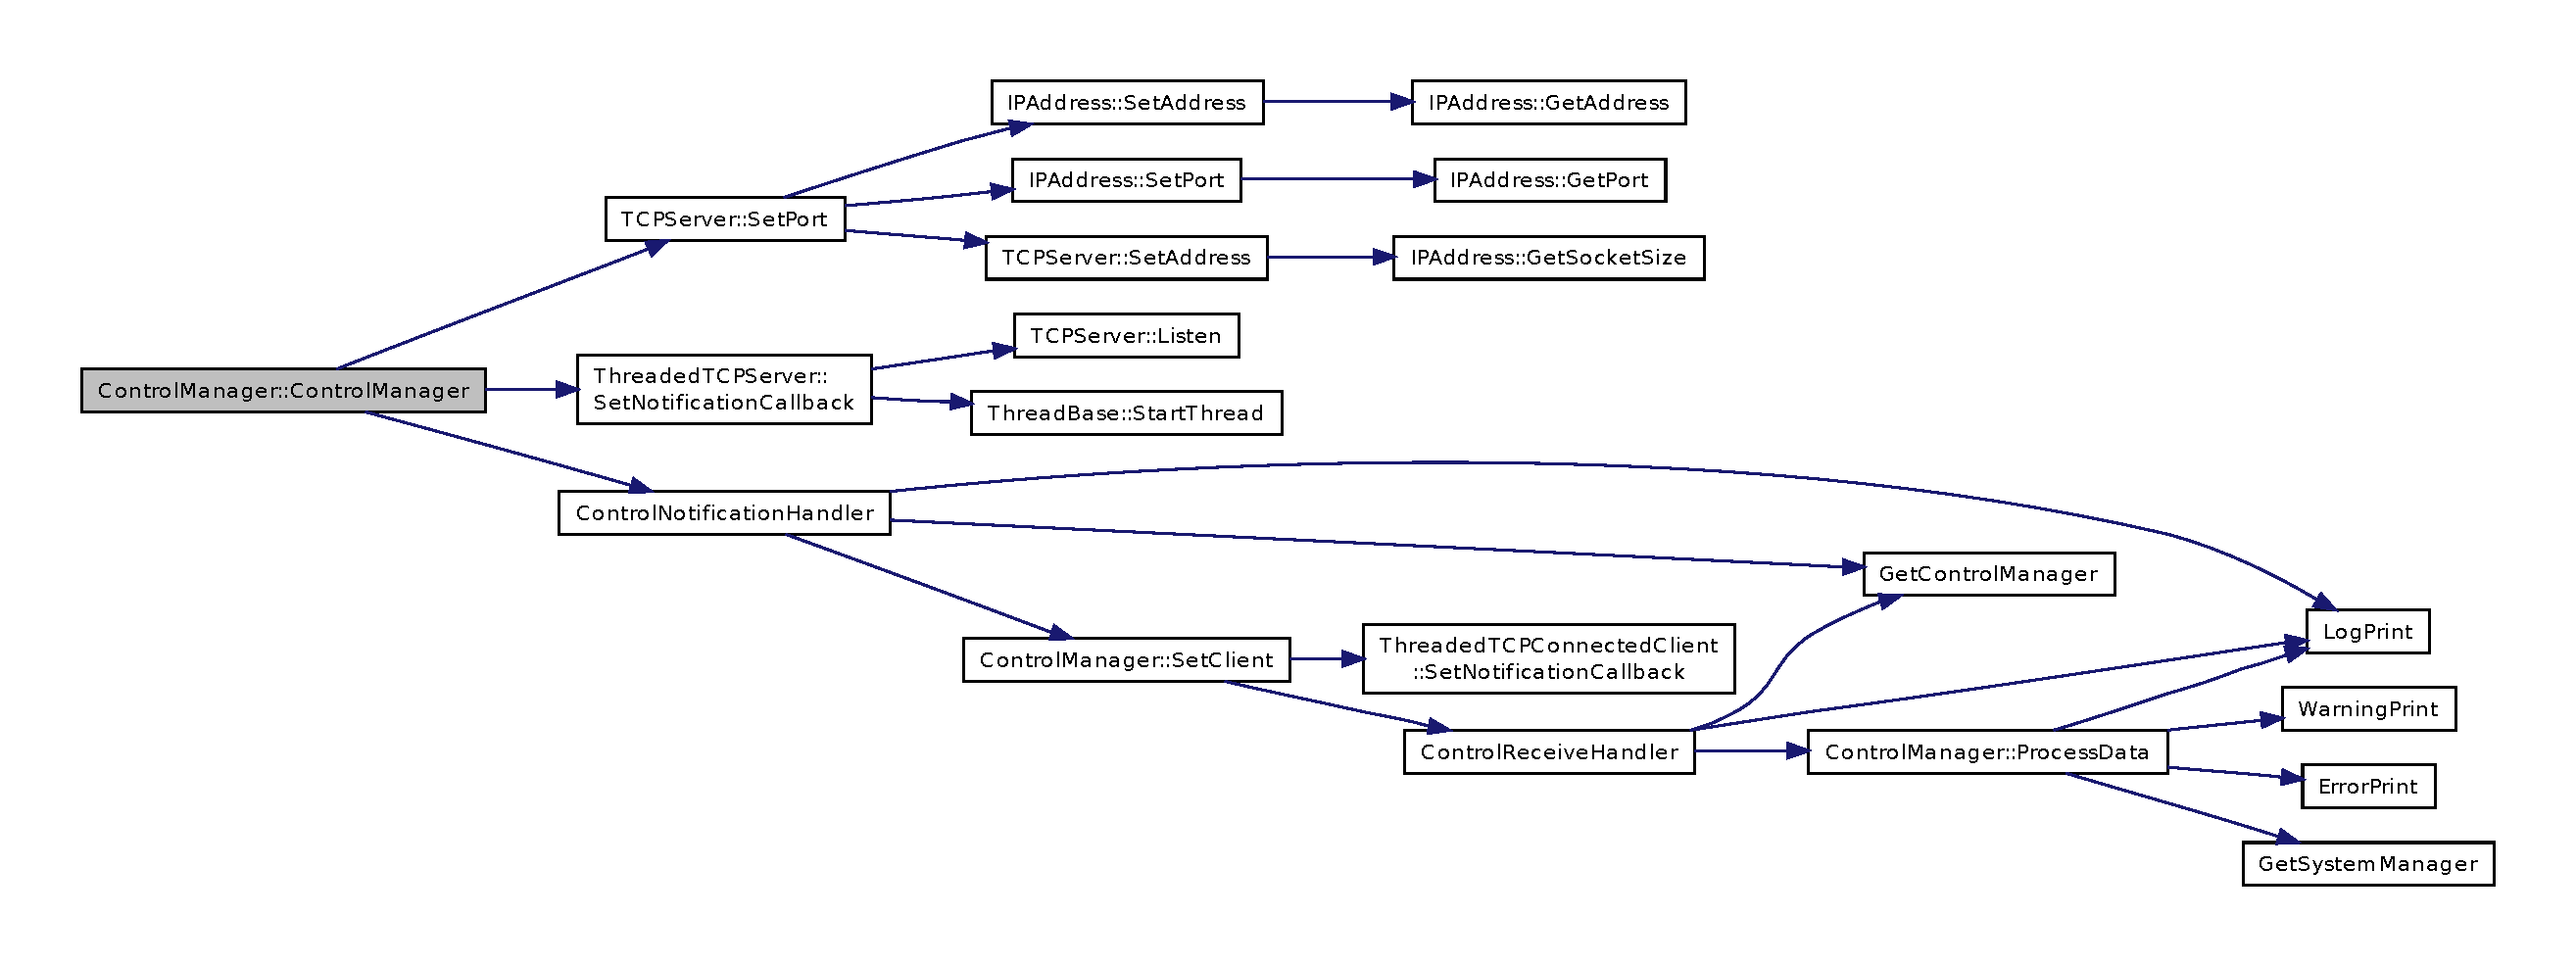
\includegraphics[width=350pt]{class_control_manager_ab81bac3e592705b7ca4b23ce473fe26e_cgraph}
\end{center}
\end{figure}




\subsection{Member Function Documentation}
\hypertarget{class_control_manager_a5b551f560431d0bb0bcf6c338bac8eb3}{\index{Control\-Manager@{Control\-Manager}!Client\-Demand\-Negotiation@{Client\-Demand\-Negotiation}}
\index{Client\-Demand\-Negotiation@{Client\-Demand\-Negotiation}!ControlManager@{Control\-Manager}}
\subsubsection[{Client\-Demand\-Negotiation}]{\setlength{\rightskip}{0pt plus 5cm}void Control\-Manager\-::\-Client\-Demand\-Negotiation (
\begin{DoxyParamCaption}
\item[{const {\bf T\-Client\-Id}}]{client\-Id, }
\item[{const {\bf T\-Number\-Of\-Data\-Points}}]{number\-Of\-Data\-Points, }
\item[{{\bf T\-Data\-Point} $\ast$}]{data\-Points}
\end{DoxyParamCaption}
)}}\label{class_control_manager_a5b551f560431d0bb0bcf6c338bac8eb3}


Definition at line 231 of file Control\-Manager.\-cpp.



Here is the call graph for this function\-:\nopagebreak
\begin{figure}[H]
\begin{center}
\leavevmode
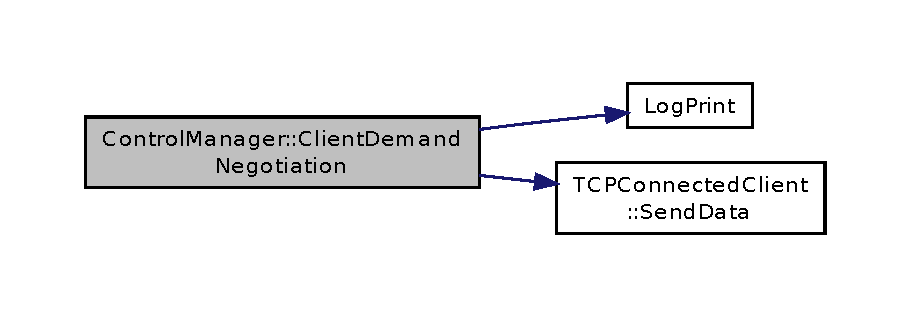
\includegraphics[width=350pt]{class_control_manager_a5b551f560431d0bb0bcf6c338bac8eb3_cgraph}
\end{center}
\end{figure}




Here is the caller graph for this function\-:\nopagebreak
\begin{figure}[H]
\begin{center}
\leavevmode
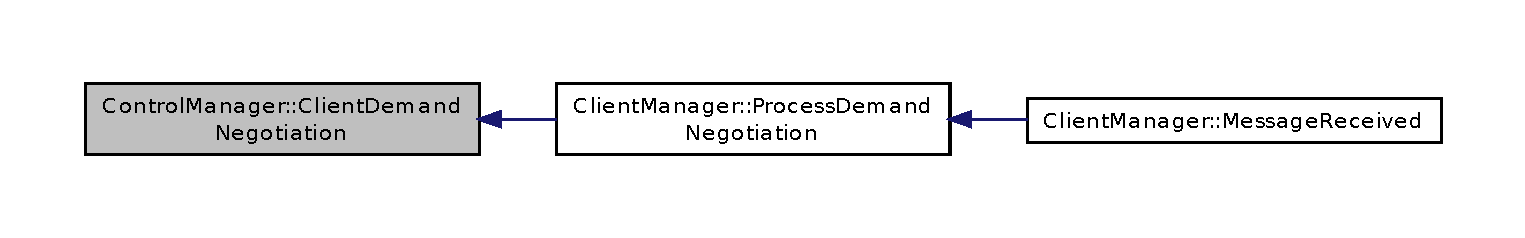
\includegraphics[width=350pt]{class_control_manager_a5b551f560431d0bb0bcf6c338bac8eb3_icgraph}
\end{center}
\end{figure}


\hypertarget{class_control_manager_aa4398a05586d9b711aa6101334deefe1}{\index{Control\-Manager@{Control\-Manager}!Client\-Price\-Request@{Client\-Price\-Request}}
\index{Client\-Price\-Request@{Client\-Price\-Request}!ControlManager@{Control\-Manager}}
\subsubsection[{Client\-Price\-Request}]{\setlength{\rightskip}{0pt plus 5cm}void Control\-Manager\-::\-Client\-Price\-Request (
\begin{DoxyParamCaption}
\item[{const {\bf T\-Client\-Id}}]{client\-Id}
\end{DoxyParamCaption}
)}}\label{class_control_manager_aa4398a05586d9b711aa6101334deefe1}


Definition at line 203 of file Control\-Manager.\-cpp.



Here is the call graph for this function\-:\nopagebreak
\begin{figure}[H]
\begin{center}
\leavevmode
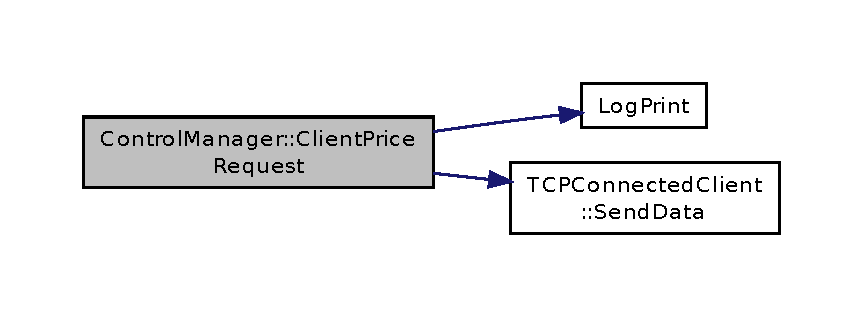
\includegraphics[width=350pt]{class_control_manager_aa4398a05586d9b711aa6101334deefe1_cgraph}
\end{center}
\end{figure}




Here is the caller graph for this function\-:\nopagebreak
\begin{figure}[H]
\begin{center}
\leavevmode
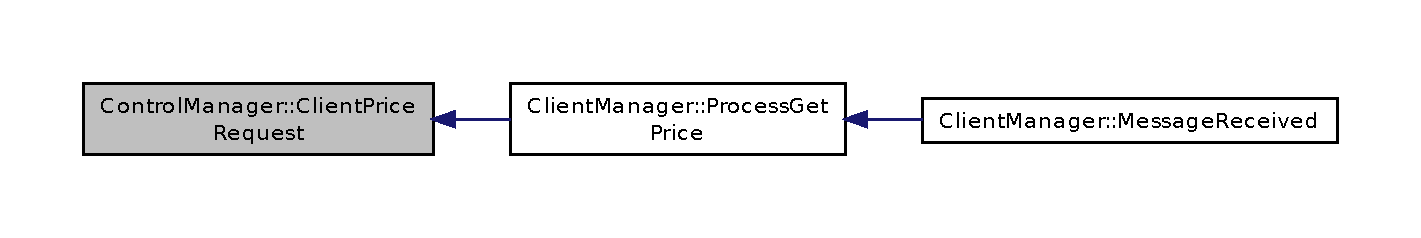
\includegraphics[width=350pt]{class_control_manager_aa4398a05586d9b711aa6101334deefe1_icgraph}
\end{center}
\end{figure}


\hypertarget{class_control_manager_a927449c3a4ba8a5bdc23e3747d5bb077}{\index{Control\-Manager@{Control\-Manager}!Get\-Client\-Name@{Get\-Client\-Name}}
\index{Get\-Client\-Name@{Get\-Client\-Name}!ControlManager@{Control\-Manager}}
\subsubsection[{Get\-Client\-Name}]{\setlength{\rightskip}{0pt plus 5cm}{\bf T\-Client\-Name} Control\-Manager\-::\-Get\-Client\-Name (
\begin{DoxyParamCaption}
\item[{const {\bf T\-Client\-Id}}]{client\-Id}
\end{DoxyParamCaption}
)\hspace{0.3cm}{\ttfamily [inline]}}}\label{class_control_manager_a927449c3a4ba8a5bdc23e3747d5bb077}


Definition at line 257 of file Control\-Manager.\-h.



Here is the call graph for this function\-:\nopagebreak
\begin{figure}[H]
\begin{center}
\leavevmode
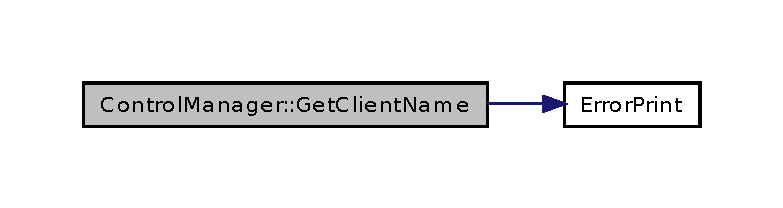
\includegraphics[width=350pt]{class_control_manager_a927449c3a4ba8a5bdc23e3747d5bb077_cgraph}
\end{center}
\end{figure}


\hypertarget{class_control_manager_a0d5212df17307aef87d42add3aa6cc7a}{\index{Control\-Manager@{Control\-Manager}!Make\-Decision@{Make\-Decision}}
\index{Make\-Decision@{Make\-Decision}!ControlManager@{Control\-Manager}}
\subsubsection[{Make\-Decision}]{\setlength{\rightskip}{0pt plus 5cm}void Control\-Manager\-::\-Make\-Decision (
\begin{DoxyParamCaption}
\item[{void}]{}
\end{DoxyParamCaption}
)}}\label{class_control_manager_a0d5212df17307aef87d42add3aa6cc7a}


Starts the decision process by sending necessary information to External Controller. 

This function starts the synchronous client decision process by sending the required information for each client. The information contains\-:
\begin{DoxyItemize}
\item Message Size for easier processing.
\item Total number of synchronous clients. 
\end{DoxyItemize}

Definition at line 132 of file Control\-Manager.\-cpp.



Here is the call graph for this function\-:\nopagebreak
\begin{figure}[H]
\begin{center}
\leavevmode
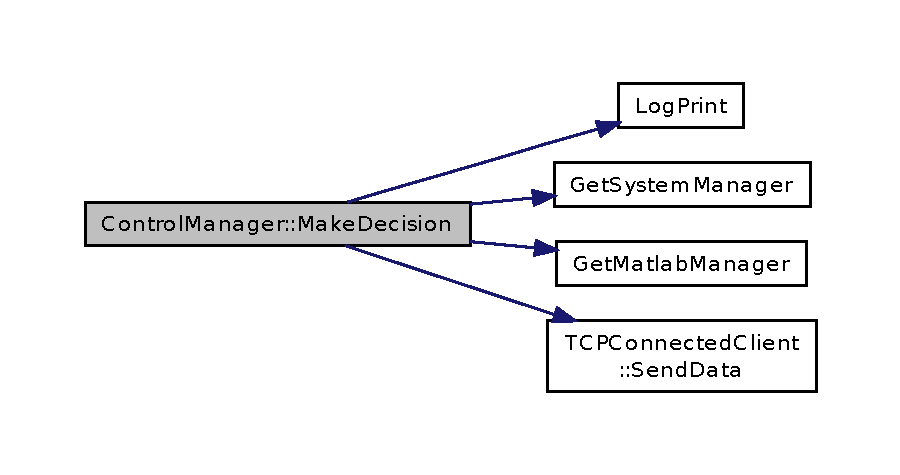
\includegraphics[width=350pt]{class_control_manager_a0d5212df17307aef87d42add3aa6cc7a_cgraph}
\end{center}
\end{figure}




Here is the caller graph for this function\-:\nopagebreak
\begin{figure}[H]
\begin{center}
\leavevmode
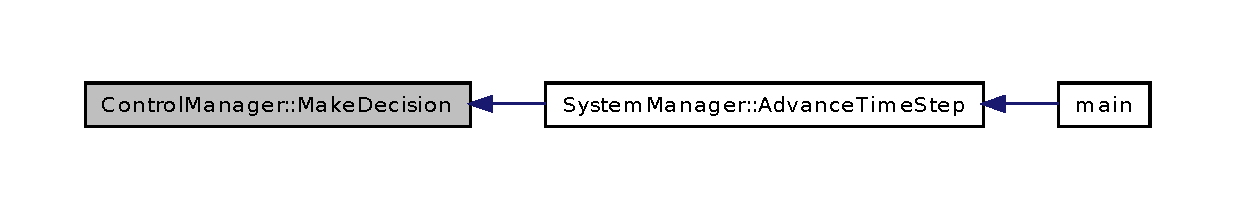
\includegraphics[width=350pt]{class_control_manager_a0d5212df17307aef87d42add3aa6cc7a_icgraph}
\end{center}
\end{figure}


\hypertarget{class_control_manager_a2dc55da1b01fd175b3d885c68b8a7524}{\index{Control\-Manager@{Control\-Manager}!Process\-Data@{Process\-Data}}
\index{Process\-Data@{Process\-Data}!ControlManager@{Control\-Manager}}
\subsubsection[{Process\-Data}]{\setlength{\rightskip}{0pt plus 5cm}void Control\-Manager\-::\-Process\-Data (
\begin{DoxyParamCaption}
\item[{void $\ast$}]{data, }
\item[{const size\-\_\-t}]{size}
\end{DoxyParamCaption}
)}}\label{class_control_manager_a2dc55da1b01fd175b3d885c68b8a7524}


Processes the received message from the External Controller. 

This function processes the received message from the External Controller. Note that the received buffer is not guaranteed to hold a single message. This function processes the buffer in a while loop until all received messages are processed in order not to lose any data. The work flow is as follows\-:
\begin{DoxyItemize}
\item Check the received size for a connection drop (gracefull or not).
\item Check the message type and process the respective data structure.
\item Repeat process until the remaining unprocessed message size is zero. \begin{DoxyRefDesc}{Todo}
\item[\hyperlink{todo__todo000002}{Todo}]Divide the function into multiple functions, processing each message separately.\end{DoxyRefDesc}



\begin{DoxyParams}{Parameters}
{\em data} & Buffer for the received message. \\
\hline
{\em size} & Size of the received message. \\
\hline
\end{DoxyParams}

\end{DoxyItemize}

Definition at line 44 of file Control\-Manager.\-cpp.



Here is the call graph for this function\-:\nopagebreak
\begin{figure}[H]
\begin{center}
\leavevmode
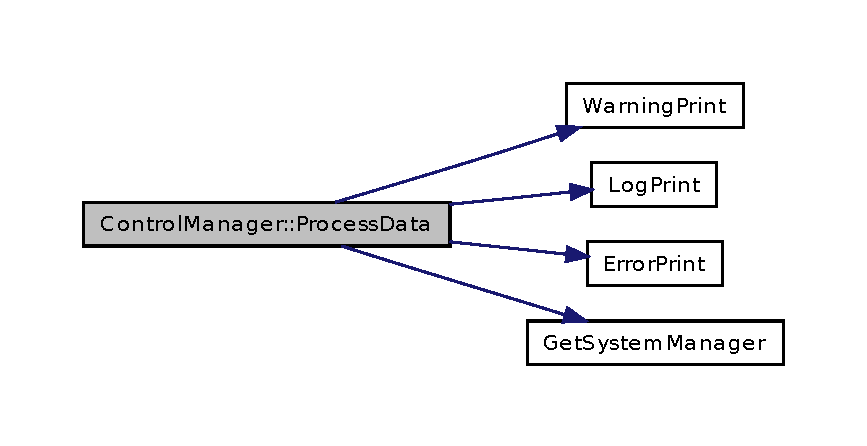
\includegraphics[width=350pt]{class_control_manager_a2dc55da1b01fd175b3d885c68b8a7524_cgraph}
\end{center}
\end{figure}




Here is the caller graph for this function\-:
\nopagebreak
\begin{figure}[H]
\begin{center}
\leavevmode
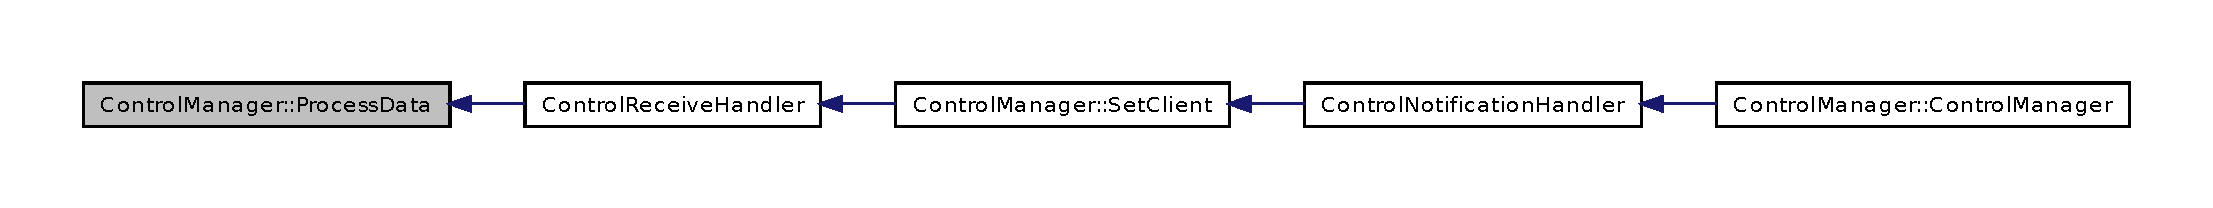
\includegraphics[width=350pt]{class_control_manager_a2dc55da1b01fd175b3d885c68b8a7524_icgraph}
\end{center}
\end{figure}


\hypertarget{class_control_manager_a56df538a5380c9091123a5a8a5e0fe86}{\index{Control\-Manager@{Control\-Manager}!Register\-Client@{Register\-Client}}
\index{Register\-Client@{Register\-Client}!ControlManager@{Control\-Manager}}
\subsubsection[{Register\-Client}]{\setlength{\rightskip}{0pt plus 5cm}void Control\-Manager\-::\-Register\-Client (
\begin{DoxyParamCaption}
\item[{const {\bf T\-Client\-Id}}]{client\-Id, }
\item[{const {\bf T\-Client\-Name} \&}]{client\-Name, }
\item[{{\bf Client\-Manager} $\ast$}]{client\-Manager}
\end{DoxyParamCaption}
)\hspace{0.3cm}{\ttfamily [inline]}}}\label{class_control_manager_a56df538a5380c9091123a5a8a5e0fe86}


Definition at line 229 of file Control\-Manager.\-h.



Here is the call graph for this function\-:\nopagebreak
\begin{figure}[H]
\begin{center}
\leavevmode
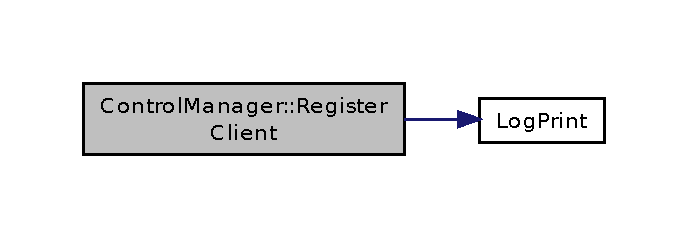
\includegraphics[width=330pt]{class_control_manager_a56df538a5380c9091123a5a8a5e0fe86_cgraph}
\end{center}
\end{figure}




Here is the caller graph for this function\-:\nopagebreak
\begin{figure}[H]
\begin{center}
\leavevmode
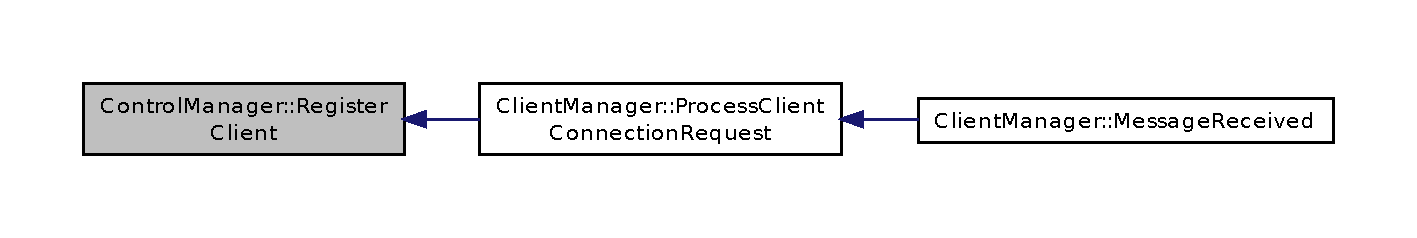
\includegraphics[width=350pt]{class_control_manager_a56df538a5380c9091123a5a8a5e0fe86_icgraph}
\end{center}
\end{figure}


\hypertarget{class_control_manager_a67d548535b36a78e315a0aa5f9f8e6c8}{\index{Control\-Manager@{Control\-Manager}!Set\-Client@{Set\-Client}}
\index{Set\-Client@{Set\-Client}!ControlManager@{Control\-Manager}}
\subsubsection[{Set\-Client}]{\setlength{\rightskip}{0pt plus 5cm}void Control\-Manager\-::\-Set\-Client (
\begin{DoxyParamCaption}
\item[{{\bf Threaded\-T\-C\-P\-Connected\-Client} $\ast$}]{client}
\end{DoxyParamCaption}
)\hspace{0.3cm}{\ttfamily [inline]}}}\label{class_control_manager_a67d548535b36a78e315a0aa5f9f8e6c8}
Sets the connection information to the accepted External Controller.


\begin{DoxyParams}{Parameters}
{\em client} & Connection information fo the newly accepted External Controller. \\
\hline
\end{DoxyParams}


Definition at line 187 of file Control\-Manager.\-h.



Here is the call graph for this function\-:
\nopagebreak
\begin{figure}[H]
\begin{center}
\leavevmode
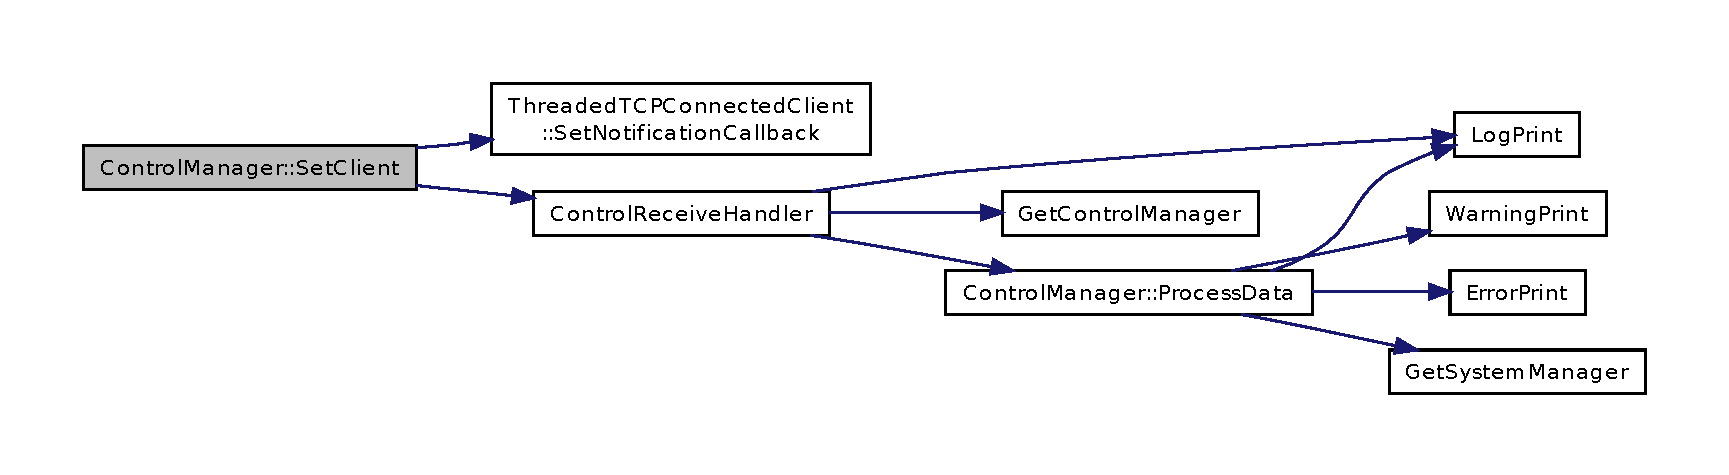
\includegraphics[width=350pt]{class_control_manager_a67d548535b36a78e315a0aa5f9f8e6c8_cgraph}
\end{center}
\end{figure}




Here is the caller graph for this function\-:\nopagebreak
\begin{figure}[H]
\begin{center}
\leavevmode
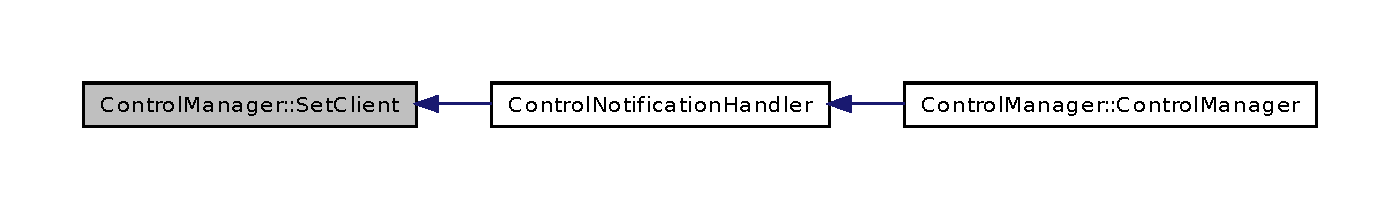
\includegraphics[width=350pt]{class_control_manager_a67d548535b36a78e315a0aa5f9f8e6c8_icgraph}
\end{center}
\end{figure}


\hypertarget{class_control_manager_ac3c913a01fe2e5e5467ad3d140c8e9a2}{\index{Control\-Manager@{Control\-Manager}!Un\-Register\-Client@{Un\-Register\-Client}}
\index{Un\-Register\-Client@{Un\-Register\-Client}!ControlManager@{Control\-Manager}}
\subsubsection[{Un\-Register\-Client}]{\setlength{\rightskip}{0pt plus 5cm}void Control\-Manager\-::\-Un\-Register\-Client (
\begin{DoxyParamCaption}
\item[{const {\bf T\-Client\-Id}}]{client\-Id}
\end{DoxyParamCaption}
)\hspace{0.3cm}{\ttfamily [inline]}}}\label{class_control_manager_ac3c913a01fe2e5e5467ad3d140c8e9a2}


Definition at line 239 of file Control\-Manager.\-h.



Here is the call graph for this function\-:\nopagebreak
\begin{figure}[H]
\begin{center}
\leavevmode
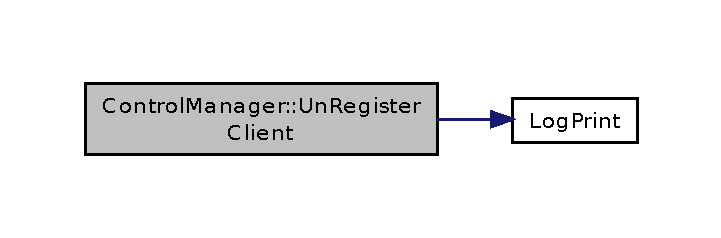
\includegraphics[width=346pt]{class_control_manager_ac3c913a01fe2e5e5467ad3d140c8e9a2_cgraph}
\end{center}
\end{figure}




Here is the caller graph for this function\-:\nopagebreak
\begin{figure}[H]
\begin{center}
\leavevmode
\includegraphics[width=350pt]{class_control_manager_ac3c913a01fe2e5e5467ad3d140c8e9a2_icgraph}
\end{center}
\end{figure}


\hypertarget{class_control_manager_a4e23ffb481554c26cf99c411dd16ae36}{\index{Control\-Manager@{Control\-Manager}!Wait\-Until\-Ready@{Wait\-Until\-Ready}}
\index{Wait\-Until\-Ready@{Wait\-Until\-Ready}!ControlManager@{Control\-Manager}}
\subsubsection[{Wait\-Until\-Ready}]{\setlength{\rightskip}{0pt plus 5cm}void Control\-Manager\-::\-Wait\-Until\-Ready (
\begin{DoxyParamCaption}
\item[{void}]{}
\end{DoxyParamCaption}
)\hspace{0.3cm}{\ttfamily [inline]}}}\label{class_control_manager_a4e23ffb481554c26cf99c411dd16ae36}


Definition at line 221 of file Control\-Manager.\-h.



Here is the caller graph for this function\-:\nopagebreak
\begin{figure}[H]
\begin{center}
\leavevmode
\includegraphics[width=350pt]{class_control_manager_a4e23ffb481554c26cf99c411dd16ae36_icgraph}
\end{center}
\end{figure}




\subsection{Friends And Related Function Documentation}
\hypertarget{class_control_manager_a63bfd4667c9c70297f25ae5e5176818e}{\index{Control\-Manager@{Control\-Manager}!Get\-Control\-Manager@{Get\-Control\-Manager}}
\index{Get\-Control\-Manager@{Get\-Control\-Manager}!ControlManager@{Control\-Manager}}
\subsubsection[{Get\-Control\-Manager}]{\setlength{\rightskip}{0pt plus 5cm}{\bf Control\-Manager}\& Get\-Control\-Manager (
\begin{DoxyParamCaption}
\item[{void}]{}
\end{DoxyParamCaption}
)\hspace{0.3cm}{\ttfamily [friend]}}}\label{class_control_manager_a63bfd4667c9c70297f25ae5e5176818e}


Returns the only instance of \hyperlink{class_control_manager}{Control\-Manager}. 

Friend method for singleton implementation.

\begin{DoxyReturn}{Returns}
Returns the reference to the \hyperlink{class_control_manager}{Control\-Manager}.

Only instance of \hyperlink{class_control_manager}{Control\-Manager}. 
\end{DoxyReturn}


Definition at line 11 of file Control\-Manager.\-cpp.



\subsection{Member Data Documentation}
\hypertarget{class_control_manager_a3081c331c70f5b08dc0ef2615d86cc55}{\index{Control\-Manager@{Control\-Manager}!m\-\_\-client@{m\-\_\-client}}
\index{m\-\_\-client@{m\-\_\-client}!ControlManager@{Control\-Manager}}
\subsubsection[{m\-\_\-client}]{\setlength{\rightskip}{0pt plus 5cm}{\bf Threaded\-T\-C\-P\-Connected\-Client}$\ast$ Control\-Manager\-::m\-\_\-client\hspace{0.3cm}{\ttfamily [private]}}}\label{class_control_manager_a3081c331c70f5b08dc0ef2615d86cc55}
Pointer to the currently accepted external controller communication handler. 

Definition at line 157 of file Control\-Manager.\-h.

\hypertarget{class_control_manager_a5623f6ef4da21d143a7a6cf5fbee136f}{\index{Control\-Manager@{Control\-Manager}!m\-\_\-client\-Id\-Map@{m\-\_\-client\-Id\-Map}}
\index{m\-\_\-client\-Id\-Map@{m\-\_\-client\-Id\-Map}!ControlManager@{Control\-Manager}}
\subsubsection[{m\-\_\-client\-Id\-Map}]{\setlength{\rightskip}{0pt plus 5cm}{\bf T\-Client\-Id\-Map} Control\-Manager\-::m\-\_\-client\-Id\-Map\hspace{0.3cm}{\ttfamily [private]}}}\label{class_control_manager_a5623f6ef4da21d143a7a6cf5fbee136f}
Map containing the unique id to object name mapping. 

Definition at line 167 of file Control\-Manager.\-h.

\hypertarget{class_control_manager_af47dee5a077190c6aeb7b9ef3d9cfb3b}{\index{Control\-Manager@{Control\-Manager}!m\-\_\-client\-Manager\-Map@{m\-\_\-client\-Manager\-Map}}
\index{m\-\_\-client\-Manager\-Map@{m\-\_\-client\-Manager\-Map}!ControlManager@{Control\-Manager}}
\subsubsection[{m\-\_\-client\-Manager\-Map}]{\setlength{\rightskip}{0pt plus 5cm}{\bf T\-Client\-Manager\-Map} Control\-Manager\-::m\-\_\-client\-Manager\-Map\hspace{0.3cm}{\ttfamily [private]}}}\label{class_control_manager_af47dee5a077190c6aeb7b9ef3d9cfb3b}
Map containing the unique id to \hyperlink{class_client_manager}{Client\-Manager} mapping. 

Definition at line 172 of file Control\-Manager.\-h.

\hypertarget{class_control_manager_ab718d2d17750dfea91411de871855075}{\index{Control\-Manager@{Control\-Manager}!m\-\_\-ready\-Semaphore@{m\-\_\-ready\-Semaphore}}
\index{m\-\_\-ready\-Semaphore@{m\-\_\-ready\-Semaphore}!ControlManager@{Control\-Manager}}
\subsubsection[{m\-\_\-ready\-Semaphore}]{\setlength{\rightskip}{0pt plus 5cm}Semaphore Control\-Manager\-::m\-\_\-ready\-Semaphore\hspace{0.3cm}{\ttfamily [private]}}}\label{class_control_manager_ab718d2d17750dfea91411de871855075}
Semaphore that is released when the frame is finished by the external controller. It stops all synchronous control until the next frame starts. This handles the process synchronization with the External Controller in a local way. 

Definition at line 162 of file Control\-Manager.\-h.

\hypertarget{class_control_manager_a1b71eabaeddfd8ec80e503b734c72e9d}{\index{Control\-Manager@{Control\-Manager}!m\-\_\-server@{m\-\_\-server}}
\index{m\-\_\-server@{m\-\_\-server}!ControlManager@{Control\-Manager}}
\subsubsection[{m\-\_\-server}]{\setlength{\rightskip}{0pt plus 5cm}{\bf Threaded\-T\-C\-P\-Server} Control\-Manager\-::m\-\_\-server\hspace{0.3cm}{\ttfamily [private]}}}\label{class_control_manager_a1b71eabaeddfd8ec80e503b734c72e9d}
Implements the T\-C\-P server for external controller communication. 

Definition at line 152 of file Control\-Manager.\-h.



The documentation for this class was generated from the following files\-:\begin{DoxyCompactItemize}
\item 
S2\-Sim/\hyperlink{_control_manager_8h}{Control\-Manager.\-h}\item 
S2\-Sim/\hyperlink{_control_manager_8cpp}{Control\-Manager.\-cpp}\end{DoxyCompactItemize}

\hypertarget{class_terra_swarm_1_1_synchronous_1_1_demand_negotiation}{\section{Terra\-Swarm\-:\-:Synchronous\-:\-:Demand\-Negotiation Class Reference}
\label{class_terra_swarm_1_1_synchronous_1_1_demand_negotiation}\index{Terra\-Swarm\-::\-Synchronous\-::\-Demand\-Negotiation@{Terra\-Swarm\-::\-Synchronous\-::\-Demand\-Negotiation}}
}


Defines the \hyperlink{class_terra_swarm_1_1_synchronous_1_1_demand_negotiation}{Demand\-Negotiation} message sent from the client to the Controller as a response to the price proposal.  




{\ttfamily \#include $<$Demand\-Negotiation.\-h$>$}

\subsection*{Public Types}
\begin{DoxyCompactItemize}
\item 
enum \hyperlink{class_terra_swarm_1_1_synchronous_1_1_demand_negotiation_a62e3d42f7a50e61a19ac2bc6349c302d}{Check\-Result\-Values} \{ \hyperlink{class_terra_swarm_1_1_synchronous_1_1_demand_negotiation_a62e3d42f7a50e61a19ac2bc6349c302da3a190a1e60e673508e7d0b752edada78}{Success} = ( T\-Check\-Result )true, 
\hyperlink{class_terra_swarm_1_1_synchronous_1_1_demand_negotiation_a62e3d42f7a50e61a19ac2bc6349c302da172b152bb4bc982cf5d623de5a1e696d}{Fail} = ( T\-Check\-Result )false
 \}
\begin{DoxyCompactList}\small\item\em Defines the values for T\-Check\-Result. \end{DoxyCompactList}\item 
typedef bool \hyperlink{class_terra_swarm_1_1_synchronous_1_1_demand_negotiation_abf70719cd7b70d3eeecb1949bc2157a3}{T\-Check\-Result}
\begin{DoxyCompactList}\small\item\em Defines the message check result type. \end{DoxyCompactList}\item 
typedef unsigned int \hyperlink{class_terra_swarm_1_1_synchronous_1_1_demand_negotiation_aeaaae7fc1861d9af2bff4c9dcb4d89ac}{T\-Number\-Of\-Data\-Points}
\begin{DoxyCompactList}\small\item\em Defines the type for number of data points. \end{DoxyCompactList}\item 
typedef unsigned int \hyperlink{class_terra_swarm_1_1_synchronous_1_1_demand_negotiation_a6660353fa0a65775070bba8571a76e3d}{T\-Data\-Point}
\begin{DoxyCompactList}\small\item\em Defines a general data point, used for consumption in this message. \end{DoxyCompactList}\end{DoxyCompactItemize}
\subsection*{Public Member Functions}
\begin{DoxyCompactItemize}
\item 
\hyperlink{class_terra_swarm_1_1_synchronous_1_1_demand_negotiation_a305449b096b0a75cc403222653b241a4}{$\sim$\-Demand\-Negotiation} (void)
\begin{DoxyCompactList}\small\item\em Deallocates the memory. \end{DoxyCompactList}\item 
\hyperlink{class_terra_swarm_1_1_synchronous_1_1_demand_negotiation_abf70719cd7b70d3eeecb1949bc2157a3}{T\-Check\-Result} \hyperlink{class_terra_swarm_1_1_synchronous_1_1_demand_negotiation_a1ebc766e094f58150ff5d1fa78031294}{Check\-Message} (void) const 
\begin{DoxyCompactList}\small\item\em Checks whether the current memory contains a \hyperlink{class_terra_swarm_1_1_synchronous_1_1_demand_negotiation}{Demand\-Negotiation} message. \end{DoxyCompactList}\item 
\hyperlink{class_terra_swarm_1_1_synchronous_1_1_demand_negotiation_aeaaae7fc1861d9af2bff4c9dcb4d89ac}{T\-Number\-Of\-Data\-Points} \hyperlink{class_terra_swarm_1_1_synchronous_1_1_demand_negotiation_af0694c36ab00a1dadf8bb8f1b3c7c159}{Get\-Number\-Of\-Data\-Points} (void) const 
\begin{DoxyCompactList}\small\item\em Reads the number of data points in the message. \end{DoxyCompactList}\item 
\hyperlink{class_terra_swarm_1_1_synchronous_1_1_demand_negotiation_a6660353fa0a65775070bba8571a76e3d}{T\-Data\-Point} $\ast$ \hyperlink{class_terra_swarm_1_1_synchronous_1_1_demand_negotiation_ab99ce665f0822299184ff34cf5e674d2}{Get\-Data\-Points} (void) const 
\begin{DoxyCompactList}\small\item\em Gets the pointer to the data points field. \end{DoxyCompactList}\end{DoxyCompactItemize}
\subsection*{Static Public Member Functions}
\begin{DoxyCompactItemize}
\item 
static \hyperlink{class_terra_swarm_1_1_synchronous_1_1_demand_negotiation}{Demand\-Negotiation} $\ast$ \hyperlink{class_terra_swarm_1_1_synchronous_1_1_demand_negotiation_a99ffac24b0af7f388d29eb47d3c19f33}{Get\-New\-Demand\-Negotiation} (const \hyperlink{class_terra_swarm_1_1_message_header_a516b36855e2aad7cfbf8770f1b42784f}{Message\-Header\-::\-T\-Sender\-Id} sender\-Id, const \hyperlink{class_terra_swarm_1_1_message_header_aa3260702b182b6f88ddbdd3416e98df0}{Message\-Header\-::\-T\-Receiver\-Id} receiver\-Id, const \hyperlink{class_terra_swarm_1_1_synchronous_1_1_demand_negotiation_aeaaae7fc1861d9af2bff4c9dcb4d89ac}{T\-Number\-Of\-Data\-Points} number\-Of\-Data\-Points, \hyperlink{class_terra_swarm_1_1_synchronous_1_1_demand_negotiation_a6660353fa0a65775070bba8571a76e3d}{T\-Data\-Point} $\ast$data\-Points)
\begin{DoxyCompactList}\small\item\em Creates a new \hyperlink{class_terra_swarm_1_1_synchronous_1_1_demand_negotiation}{Demand\-Negotiation} message and allocates the memory. \end{DoxyCompactList}\end{DoxyCompactItemize}
\subsection*{Private Types}
\begin{DoxyCompactItemize}
\item 
enum \hyperlink{class_terra_swarm_1_1_synchronous_1_1_demand_negotiation_afbf936743aecc68e9e53598ed8146e21}{Header\-Values} \{ \hyperlink{class_terra_swarm_1_1_synchronous_1_1_demand_negotiation_afbf936743aecc68e9e53598ed8146e21a6c276b43db55c33b12b96bf8103aeccc}{Message\-Type} = 0x0003, 
\hyperlink{class_terra_swarm_1_1_synchronous_1_1_demand_negotiation_afbf936743aecc68e9e53598ed8146e21a19ff4bbd69f6d5e53a2c8ec3c7e6c582}{Message\-Id} = 0x0004
 \}
\begin{DoxyCompactList}\small\item\em Message Header values. \end{DoxyCompactList}\item 
enum \hyperlink{class_terra_swarm_1_1_synchronous_1_1_demand_negotiation_a4e1d77efc7d917053f43b4e7faf6dfa3}{Field\-Size\-Values} \{ \hyperlink{class_terra_swarm_1_1_synchronous_1_1_demand_negotiation_a4e1d77efc7d917053f43b4e7faf6dfa3a177cce271c67adfe880026f2991ddd24}{Number\-Of\-Data\-Points\-Size} = sizeof( T\-Number\-Of\-Data\-Points ), 
\hyperlink{class_terra_swarm_1_1_synchronous_1_1_demand_negotiation_a4e1d77efc7d917053f43b4e7faf6dfa3a98cb806c46ea5332ce3f6e2bc2c77b86}{Data\-Point\-Size} = sizeof( T\-Data\-Point )
 \}
\begin{DoxyCompactList}\small\item\em Size of the fields in the message. \end{DoxyCompactList}\item 
enum \hyperlink{class_terra_swarm_1_1_synchronous_1_1_demand_negotiation_a28b34eef9d480a2368260c99ecc487bf}{Field\-Index\-Values} \{ \hyperlink{class_terra_swarm_1_1_synchronous_1_1_demand_negotiation_a28b34eef9d480a2368260c99ecc487bfafbea2a0f9ecc4bd089bb5fae8be2777b}{Number\-Of\-Data\-Points\-Index} = Message\-Header\-:\-:Message\-Header\-Size, 
\hyperlink{class_terra_swarm_1_1_synchronous_1_1_demand_negotiation_a28b34eef9d480a2368260c99ecc487bfa87d6d357dd529ff7f9503d69dd044a5b}{Data\-Start\-Index} = Number\-Of\-Data\-Points\-Index + Number\-Of\-Data\-Points\-Size
 \}
\begin{DoxyCompactList}\small\item\em Index of the fields in the message. \end{DoxyCompactList}\item 
typedef \hyperlink{class_terra_swarm_1_1_network_byte_accessor}{Network\-Byte\-Accessor}\\*
$<$ \hyperlink{class_terra_swarm_1_1_synchronous_1_1_demand_negotiation_a28b34eef9d480a2368260c99ecc487bfafbea2a0f9ecc4bd089bb5fae8be2777b}{Number\-Of\-Data\-Points\-Index}, \\*
\hyperlink{class_terra_swarm_1_1_synchronous_1_1_demand_negotiation_a4e1d77efc7d917053f43b4e7faf6dfa3a177cce271c67adfe880026f2991ddd24}{Number\-Of\-Data\-Points\-Size} $>$ \hyperlink{class_terra_swarm_1_1_synchronous_1_1_demand_negotiation_a86cc2804c82d511a7b9e037d041236bd}{T\-Number\-Of\-Data\-Points\-Accessor}
\begin{DoxyCompactList}\small\item\em Accessor Helper for Number\-Of\-Data\-Points field. \end{DoxyCompactList}\end{DoxyCompactItemize}
\subsection*{Private Member Functions}
\begin{DoxyCompactItemize}
\item 
\hyperlink{class_terra_swarm_1_1_synchronous_1_1_demand_negotiation_a9477added06c203f17f43cbfbd651fc4}{Demand\-Negotiation} (void)
\begin{DoxyCompactList}\small\item\em Private constructor to force the usage of the static creation method. \end{DoxyCompactList}\end{DoxyCompactItemize}


\subsection{Detailed Description}
Defines the \hyperlink{class_terra_swarm_1_1_synchronous_1_1_demand_negotiation}{Demand\-Negotiation} message sent from the client to the Controller as a response to the price proposal. 

Definition at line 23 of file Demand\-Negotiation.\-h.



\subsection{Member Typedef Documentation}
\hypertarget{class_terra_swarm_1_1_synchronous_1_1_demand_negotiation_abf70719cd7b70d3eeecb1949bc2157a3}{\index{Terra\-Swarm\-::\-Synchronous\-::\-Demand\-Negotiation@{Terra\-Swarm\-::\-Synchronous\-::\-Demand\-Negotiation}!T\-Check\-Result@{T\-Check\-Result}}
\index{T\-Check\-Result@{T\-Check\-Result}!TerraSwarm::Synchronous::DemandNegotiation@{Terra\-Swarm\-::\-Synchronous\-::\-Demand\-Negotiation}}
\subsubsection[{T\-Check\-Result}]{\setlength{\rightskip}{0pt plus 5cm}typedef bool {\bf Terra\-Swarm\-::\-Synchronous\-::\-Demand\-Negotiation\-::\-T\-Check\-Result}}}\label{class_terra_swarm_1_1_synchronous_1_1_demand_negotiation_abf70719cd7b70d3eeecb1949bc2157a3}


Defines the message check result type. 



Definition at line 39 of file Demand\-Negotiation.\-h.

\hypertarget{class_terra_swarm_1_1_synchronous_1_1_demand_negotiation_a6660353fa0a65775070bba8571a76e3d}{\index{Terra\-Swarm\-::\-Synchronous\-::\-Demand\-Negotiation@{Terra\-Swarm\-::\-Synchronous\-::\-Demand\-Negotiation}!T\-Data\-Point@{T\-Data\-Point}}
\index{T\-Data\-Point@{T\-Data\-Point}!TerraSwarm::Synchronous::DemandNegotiation@{Terra\-Swarm\-::\-Synchronous\-::\-Demand\-Negotiation}}
\subsubsection[{T\-Data\-Point}]{\setlength{\rightskip}{0pt plus 5cm}typedef unsigned int {\bf Terra\-Swarm\-::\-Synchronous\-::\-Demand\-Negotiation\-::\-T\-Data\-Point}}}\label{class_terra_swarm_1_1_synchronous_1_1_demand_negotiation_a6660353fa0a65775070bba8571a76e3d}


Defines a general data point, used for consumption in this message. 



Definition at line 58 of file Demand\-Negotiation.\-h.

\hypertarget{class_terra_swarm_1_1_synchronous_1_1_demand_negotiation_aeaaae7fc1861d9af2bff4c9dcb4d89ac}{\index{Terra\-Swarm\-::\-Synchronous\-::\-Demand\-Negotiation@{Terra\-Swarm\-::\-Synchronous\-::\-Demand\-Negotiation}!T\-Number\-Of\-Data\-Points@{T\-Number\-Of\-Data\-Points}}
\index{T\-Number\-Of\-Data\-Points@{T\-Number\-Of\-Data\-Points}!TerraSwarm::Synchronous::DemandNegotiation@{Terra\-Swarm\-::\-Synchronous\-::\-Demand\-Negotiation}}
\subsubsection[{T\-Number\-Of\-Data\-Points}]{\setlength{\rightskip}{0pt plus 5cm}typedef unsigned int {\bf Terra\-Swarm\-::\-Synchronous\-::\-Demand\-Negotiation\-::\-T\-Number\-Of\-Data\-Points}}}\label{class_terra_swarm_1_1_synchronous_1_1_demand_negotiation_aeaaae7fc1861d9af2bff4c9dcb4d89ac}


Defines the type for number of data points. 



Definition at line 53 of file Demand\-Negotiation.\-h.

\hypertarget{class_terra_swarm_1_1_synchronous_1_1_demand_negotiation_a86cc2804c82d511a7b9e037d041236bd}{\index{Terra\-Swarm\-::\-Synchronous\-::\-Demand\-Negotiation@{Terra\-Swarm\-::\-Synchronous\-::\-Demand\-Negotiation}!T\-Number\-Of\-Data\-Points\-Accessor@{T\-Number\-Of\-Data\-Points\-Accessor}}
\index{T\-Number\-Of\-Data\-Points\-Accessor@{T\-Number\-Of\-Data\-Points\-Accessor}!TerraSwarm::Synchronous::DemandNegotiation@{Terra\-Swarm\-::\-Synchronous\-::\-Demand\-Negotiation}}
\subsubsection[{T\-Number\-Of\-Data\-Points\-Accessor}]{\setlength{\rightskip}{0pt plus 5cm}typedef {\bf Network\-Byte\-Accessor}$<${\bf Number\-Of\-Data\-Points\-Index}, {\bf Number\-Of\-Data\-Points\-Size}$>$ {\bf Terra\-Swarm\-::\-Synchronous\-::\-Demand\-Negotiation\-::\-T\-Number\-Of\-Data\-Points\-Accessor}\hspace{0.3cm}{\ttfamily [private]}}}\label{class_terra_swarm_1_1_synchronous_1_1_demand_negotiation_a86cc2804c82d511a7b9e037d041236bd}


Accessor Helper for Number\-Of\-Data\-Points field. 



Definition at line 82 of file Demand\-Negotiation.\-h.



\subsection{Member Enumeration Documentation}
\hypertarget{class_terra_swarm_1_1_synchronous_1_1_demand_negotiation_a62e3d42f7a50e61a19ac2bc6349c302d}{\index{Terra\-Swarm\-::\-Synchronous\-::\-Demand\-Negotiation@{Terra\-Swarm\-::\-Synchronous\-::\-Demand\-Negotiation}!Check\-Result\-Values@{Check\-Result\-Values}}
\index{Check\-Result\-Values@{Check\-Result\-Values}!TerraSwarm::Synchronous::DemandNegotiation@{Terra\-Swarm\-::\-Synchronous\-::\-Demand\-Negotiation}}
\subsubsection[{Check\-Result\-Values}]{\setlength{\rightskip}{0pt plus 5cm}enum {\bf Terra\-Swarm\-::\-Synchronous\-::\-Demand\-Negotiation\-::\-Check\-Result\-Values}}}\label{class_terra_swarm_1_1_synchronous_1_1_demand_negotiation_a62e3d42f7a50e61a19ac2bc6349c302d}


Defines the values for T\-Check\-Result. 

\begin{Desc}
\item[Enumerator]\par
\begin{description}
\index{Success@{Success}!Terra\-Swarm\-::\-Synchronous\-::\-Demand\-Negotiation@{Terra\-Swarm\-::\-Synchronous\-::\-Demand\-Negotiation}}\index{Terra\-Swarm\-::\-Synchronous\-::\-Demand\-Negotiation@{Terra\-Swarm\-::\-Synchronous\-::\-Demand\-Negotiation}!Success@{Success}}\item[{\em 
\hypertarget{class_terra_swarm_1_1_synchronous_1_1_demand_negotiation_a62e3d42f7a50e61a19ac2bc6349c302da3a190a1e60e673508e7d0b752edada78}{Success}\label{class_terra_swarm_1_1_synchronous_1_1_demand_negotiation_a62e3d42f7a50e61a19ac2bc6349c302da3a190a1e60e673508e7d0b752edada78}
}]Message is of correct type and id. \index{Fail@{Fail}!Terra\-Swarm\-::\-Synchronous\-::\-Demand\-Negotiation@{Terra\-Swarm\-::\-Synchronous\-::\-Demand\-Negotiation}}\index{Terra\-Swarm\-::\-Synchronous\-::\-Demand\-Negotiation@{Terra\-Swarm\-::\-Synchronous\-::\-Demand\-Negotiation}!Fail@{Fail}}\item[{\em 
\hypertarget{class_terra_swarm_1_1_synchronous_1_1_demand_negotiation_a62e3d42f7a50e61a19ac2bc6349c302da172b152bb4bc982cf5d623de5a1e696d}{Fail}\label{class_terra_swarm_1_1_synchronous_1_1_demand_negotiation_a62e3d42f7a50e61a19ac2bc6349c302da172b152bb4bc982cf5d623de5a1e696d}
}]Message has incorrect type or id. \end{description}
\end{Desc}


Definition at line 44 of file Demand\-Negotiation.\-h.

\hypertarget{class_terra_swarm_1_1_synchronous_1_1_demand_negotiation_a28b34eef9d480a2368260c99ecc487bf}{\index{Terra\-Swarm\-::\-Synchronous\-::\-Demand\-Negotiation@{Terra\-Swarm\-::\-Synchronous\-::\-Demand\-Negotiation}!Field\-Index\-Values@{Field\-Index\-Values}}
\index{Field\-Index\-Values@{Field\-Index\-Values}!TerraSwarm::Synchronous::DemandNegotiation@{Terra\-Swarm\-::\-Synchronous\-::\-Demand\-Negotiation}}
\subsubsection[{Field\-Index\-Values}]{\setlength{\rightskip}{0pt plus 5cm}enum {\bf Terra\-Swarm\-::\-Synchronous\-::\-Demand\-Negotiation\-::\-Field\-Index\-Values}\hspace{0.3cm}{\ttfamily [private]}}}\label{class_terra_swarm_1_1_synchronous_1_1_demand_negotiation_a28b34eef9d480a2368260c99ecc487bf}


Index of the fields in the message. 

\begin{Desc}
\item[Enumerator]\par
\begin{description}
\index{Number\-Of\-Data\-Points\-Index@{Number\-Of\-Data\-Points\-Index}!Terra\-Swarm\-::\-Synchronous\-::\-Demand\-Negotiation@{Terra\-Swarm\-::\-Synchronous\-::\-Demand\-Negotiation}}\index{Terra\-Swarm\-::\-Synchronous\-::\-Demand\-Negotiation@{Terra\-Swarm\-::\-Synchronous\-::\-Demand\-Negotiation}!Number\-Of\-Data\-Points\-Index@{Number\-Of\-Data\-Points\-Index}}\item[{\em 
\hypertarget{class_terra_swarm_1_1_synchronous_1_1_demand_negotiation_a28b34eef9d480a2368260c99ecc487bfafbea2a0f9ecc4bd089bb5fae8be2777b}{Number\-Of\-Data\-Points\-Index}\label{class_terra_swarm_1_1_synchronous_1_1_demand_negotiation_a28b34eef9d480a2368260c99ecc487bfafbea2a0f9ecc4bd089bb5fae8be2777b}
}]\index{Data\-Start\-Index@{Data\-Start\-Index}!Terra\-Swarm\-::\-Synchronous\-::\-Demand\-Negotiation@{Terra\-Swarm\-::\-Synchronous\-::\-Demand\-Negotiation}}\index{Terra\-Swarm\-::\-Synchronous\-::\-Demand\-Negotiation@{Terra\-Swarm\-::\-Synchronous\-::\-Demand\-Negotiation}!Data\-Start\-Index@{Data\-Start\-Index}}\item[{\em 
\hypertarget{class_terra_swarm_1_1_synchronous_1_1_demand_negotiation_a28b34eef9d480a2368260c99ecc487bfa87d6d357dd529ff7f9503d69dd044a5b}{Data\-Start\-Index}\label{class_terra_swarm_1_1_synchronous_1_1_demand_negotiation_a28b34eef9d480a2368260c99ecc487bfa87d6d357dd529ff7f9503d69dd044a5b}
}]\end{description}
\end{Desc}


Definition at line 73 of file Demand\-Negotiation.\-h.

\hypertarget{class_terra_swarm_1_1_synchronous_1_1_demand_negotiation_a4e1d77efc7d917053f43b4e7faf6dfa3}{\index{Terra\-Swarm\-::\-Synchronous\-::\-Demand\-Negotiation@{Terra\-Swarm\-::\-Synchronous\-::\-Demand\-Negotiation}!Field\-Size\-Values@{Field\-Size\-Values}}
\index{Field\-Size\-Values@{Field\-Size\-Values}!TerraSwarm::Synchronous::DemandNegotiation@{Terra\-Swarm\-::\-Synchronous\-::\-Demand\-Negotiation}}
\subsubsection[{Field\-Size\-Values}]{\setlength{\rightskip}{0pt plus 5cm}enum {\bf Terra\-Swarm\-::\-Synchronous\-::\-Demand\-Negotiation\-::\-Field\-Size\-Values}\hspace{0.3cm}{\ttfamily [private]}}}\label{class_terra_swarm_1_1_synchronous_1_1_demand_negotiation_a4e1d77efc7d917053f43b4e7faf6dfa3}


Size of the fields in the message. 

\begin{Desc}
\item[Enumerator]\par
\begin{description}
\index{Number\-Of\-Data\-Points\-Size@{Number\-Of\-Data\-Points\-Size}!Terra\-Swarm\-::\-Synchronous\-::\-Demand\-Negotiation@{Terra\-Swarm\-::\-Synchronous\-::\-Demand\-Negotiation}}\index{Terra\-Swarm\-::\-Synchronous\-::\-Demand\-Negotiation@{Terra\-Swarm\-::\-Synchronous\-::\-Demand\-Negotiation}!Number\-Of\-Data\-Points\-Size@{Number\-Of\-Data\-Points\-Size}}\item[{\em 
\hypertarget{class_terra_swarm_1_1_synchronous_1_1_demand_negotiation_a4e1d77efc7d917053f43b4e7faf6dfa3a177cce271c67adfe880026f2991ddd24}{Number\-Of\-Data\-Points\-Size}\label{class_terra_swarm_1_1_synchronous_1_1_demand_negotiation_a4e1d77efc7d917053f43b4e7faf6dfa3a177cce271c67adfe880026f2991ddd24}
}]\index{Data\-Point\-Size@{Data\-Point\-Size}!Terra\-Swarm\-::\-Synchronous\-::\-Demand\-Negotiation@{Terra\-Swarm\-::\-Synchronous\-::\-Demand\-Negotiation}}\index{Terra\-Swarm\-::\-Synchronous\-::\-Demand\-Negotiation@{Terra\-Swarm\-::\-Synchronous\-::\-Demand\-Negotiation}!Data\-Point\-Size@{Data\-Point\-Size}}\item[{\em 
\hypertarget{class_terra_swarm_1_1_synchronous_1_1_demand_negotiation_a4e1d77efc7d917053f43b4e7faf6dfa3a98cb806c46ea5332ce3f6e2bc2c77b86}{Data\-Point\-Size}\label{class_terra_swarm_1_1_synchronous_1_1_demand_negotiation_a4e1d77efc7d917053f43b4e7faf6dfa3a98cb806c46ea5332ce3f6e2bc2c77b86}
}]\end{description}
\end{Desc}


Definition at line 64 of file Demand\-Negotiation.\-h.

\hypertarget{class_terra_swarm_1_1_synchronous_1_1_demand_negotiation_afbf936743aecc68e9e53598ed8146e21}{\index{Terra\-Swarm\-::\-Synchronous\-::\-Demand\-Negotiation@{Terra\-Swarm\-::\-Synchronous\-::\-Demand\-Negotiation}!Header\-Values@{Header\-Values}}
\index{Header\-Values@{Header\-Values}!TerraSwarm::Synchronous::DemandNegotiation@{Terra\-Swarm\-::\-Synchronous\-::\-Demand\-Negotiation}}
\subsubsection[{Header\-Values}]{\setlength{\rightskip}{0pt plus 5cm}enum {\bf Terra\-Swarm\-::\-Synchronous\-::\-Demand\-Negotiation\-::\-Header\-Values}\hspace{0.3cm}{\ttfamily [private]}}}\label{class_terra_swarm_1_1_synchronous_1_1_demand_negotiation_afbf936743aecc68e9e53598ed8146e21}


Message Header values. 

\begin{Desc}
\item[Enumerator]\par
\begin{description}
\index{Message\-Type@{Message\-Type}!Terra\-Swarm\-::\-Synchronous\-::\-Demand\-Negotiation@{Terra\-Swarm\-::\-Synchronous\-::\-Demand\-Negotiation}}\index{Terra\-Swarm\-::\-Synchronous\-::\-Demand\-Negotiation@{Terra\-Swarm\-::\-Synchronous\-::\-Demand\-Negotiation}!Message\-Type@{Message\-Type}}\item[{\em 
\hypertarget{class_terra_swarm_1_1_synchronous_1_1_demand_negotiation_afbf936743aecc68e9e53598ed8146e21a6c276b43db55c33b12b96bf8103aeccc}{Message\-Type}\label{class_terra_swarm_1_1_synchronous_1_1_demand_negotiation_afbf936743aecc68e9e53598ed8146e21a6c276b43db55c33b12b96bf8103aeccc}
}]\index{Message\-Id@{Message\-Id}!Terra\-Swarm\-::\-Synchronous\-::\-Demand\-Negotiation@{Terra\-Swarm\-::\-Synchronous\-::\-Demand\-Negotiation}}\index{Terra\-Swarm\-::\-Synchronous\-::\-Demand\-Negotiation@{Terra\-Swarm\-::\-Synchronous\-::\-Demand\-Negotiation}!Message\-Id@{Message\-Id}}\item[{\em 
\hypertarget{class_terra_swarm_1_1_synchronous_1_1_demand_negotiation_afbf936743aecc68e9e53598ed8146e21a19ff4bbd69f6d5e53a2c8ec3c7e6c582}{Message\-Id}\label{class_terra_swarm_1_1_synchronous_1_1_demand_negotiation_afbf936743aecc68e9e53598ed8146e21a19ff4bbd69f6d5e53a2c8ec3c7e6c582}
}]\end{description}
\end{Desc}


Definition at line 29 of file Demand\-Negotiation.\-h.



\subsection{Constructor \& Destructor Documentation}
\hypertarget{class_terra_swarm_1_1_synchronous_1_1_demand_negotiation_a9477added06c203f17f43cbfbd651fc4}{\index{Terra\-Swarm\-::\-Synchronous\-::\-Demand\-Negotiation@{Terra\-Swarm\-::\-Synchronous\-::\-Demand\-Negotiation}!Demand\-Negotiation@{Demand\-Negotiation}}
\index{Demand\-Negotiation@{Demand\-Negotiation}!TerraSwarm::Synchronous::DemandNegotiation@{Terra\-Swarm\-::\-Synchronous\-::\-Demand\-Negotiation}}
\subsubsection[{Demand\-Negotiation}]{\setlength{\rightskip}{0pt plus 5cm}Terra\-Swarm\-::\-Synchronous\-::\-Demand\-Negotiation\-::\-Demand\-Negotiation (
\begin{DoxyParamCaption}
\item[{void}]{}
\end{DoxyParamCaption}
)\hspace{0.3cm}{\ttfamily [private]}}}\label{class_terra_swarm_1_1_synchronous_1_1_demand_negotiation_a9477added06c203f17f43cbfbd651fc4}


Private constructor to force the usage of the static creation method. 



Definition at line 14 of file Demand\-Negotiation.\-cpp.

\hypertarget{class_terra_swarm_1_1_synchronous_1_1_demand_negotiation_a305449b096b0a75cc403222653b241a4}{\index{Terra\-Swarm\-::\-Synchronous\-::\-Demand\-Negotiation@{Terra\-Swarm\-::\-Synchronous\-::\-Demand\-Negotiation}!$\sim$\-Demand\-Negotiation@{$\sim$\-Demand\-Negotiation}}
\index{$\sim$\-Demand\-Negotiation@{$\sim$\-Demand\-Negotiation}!TerraSwarm::Synchronous::DemandNegotiation@{Terra\-Swarm\-::\-Synchronous\-::\-Demand\-Negotiation}}
\subsubsection[{$\sim$\-Demand\-Negotiation}]{\setlength{\rightskip}{0pt plus 5cm}Terra\-Swarm\-::\-Synchronous\-::\-Demand\-Negotiation\-::$\sim$\-Demand\-Negotiation (
\begin{DoxyParamCaption}
\item[{void}]{}
\end{DoxyParamCaption}
)}}\label{class_terra_swarm_1_1_synchronous_1_1_demand_negotiation_a305449b096b0a75cc403222653b241a4}


Deallocates the memory. 



Definition at line 18 of file Demand\-Negotiation.\-cpp.



\subsection{Member Function Documentation}
\hypertarget{class_terra_swarm_1_1_synchronous_1_1_demand_negotiation_a1ebc766e094f58150ff5d1fa78031294}{\index{Terra\-Swarm\-::\-Synchronous\-::\-Demand\-Negotiation@{Terra\-Swarm\-::\-Synchronous\-::\-Demand\-Negotiation}!Check\-Message@{Check\-Message}}
\index{Check\-Message@{Check\-Message}!TerraSwarm::Synchronous::DemandNegotiation@{Terra\-Swarm\-::\-Synchronous\-::\-Demand\-Negotiation}}
\subsubsection[{Check\-Message}]{\setlength{\rightskip}{0pt plus 5cm}{\bf Demand\-Negotiation\-::\-T\-Check\-Result} Terra\-Swarm\-::\-Synchronous\-::\-Demand\-Negotiation\-::\-Check\-Message (
\begin{DoxyParamCaption}
\item[{void}]{}
\end{DoxyParamCaption}
) const}}\label{class_terra_swarm_1_1_synchronous_1_1_demand_negotiation_a1ebc766e094f58150ff5d1fa78031294}


Checks whether the current memory contains a \hyperlink{class_terra_swarm_1_1_synchronous_1_1_demand_negotiation}{Demand\-Negotiation} message. 

\begin{DoxyReturn}{Returns}
Result of the check. 
\end{DoxyReturn}


Definition at line 42 of file Demand\-Negotiation.\-cpp.

\hypertarget{class_terra_swarm_1_1_synchronous_1_1_demand_negotiation_ab99ce665f0822299184ff34cf5e674d2}{\index{Terra\-Swarm\-::\-Synchronous\-::\-Demand\-Negotiation@{Terra\-Swarm\-::\-Synchronous\-::\-Demand\-Negotiation}!Get\-Data\-Points@{Get\-Data\-Points}}
\index{Get\-Data\-Points@{Get\-Data\-Points}!TerraSwarm::Synchronous::DemandNegotiation@{Terra\-Swarm\-::\-Synchronous\-::\-Demand\-Negotiation}}
\subsubsection[{Get\-Data\-Points}]{\setlength{\rightskip}{0pt plus 5cm}{\bf Demand\-Negotiation\-::\-T\-Data\-Point} $\ast$ Terra\-Swarm\-::\-Synchronous\-::\-Demand\-Negotiation\-::\-Get\-Data\-Points (
\begin{DoxyParamCaption}
\item[{void}]{}
\end{DoxyParamCaption}
) const}}\label{class_terra_swarm_1_1_synchronous_1_1_demand_negotiation_ab99ce665f0822299184ff34cf5e674d2}


Gets the pointer to the data points field. 

\begin{DoxyReturn}{Returns}
Pointer to the start of the data points field. 
\end{DoxyReturn}


Definition at line 61 of file Demand\-Negotiation.\-cpp.



Here is the call graph for this function\-:\nopagebreak
\begin{figure}[H]
\begin{center}
\leavevmode
\includegraphics[width=350pt]{class_terra_swarm_1_1_synchronous_1_1_demand_negotiation_ab99ce665f0822299184ff34cf5e674d2_cgraph}
\end{center}
\end{figure}




Here is the caller graph for this function\-:\nopagebreak
\begin{figure}[H]
\begin{center}
\leavevmode
\includegraphics[width=350pt]{class_terra_swarm_1_1_synchronous_1_1_demand_negotiation_ab99ce665f0822299184ff34cf5e674d2_icgraph}
\end{center}
\end{figure}


\hypertarget{class_terra_swarm_1_1_synchronous_1_1_demand_negotiation_a99ffac24b0af7f388d29eb47d3c19f33}{\index{Terra\-Swarm\-::\-Synchronous\-::\-Demand\-Negotiation@{Terra\-Swarm\-::\-Synchronous\-::\-Demand\-Negotiation}!Get\-New\-Demand\-Negotiation@{Get\-New\-Demand\-Negotiation}}
\index{Get\-New\-Demand\-Negotiation@{Get\-New\-Demand\-Negotiation}!TerraSwarm::Synchronous::DemandNegotiation@{Terra\-Swarm\-::\-Synchronous\-::\-Demand\-Negotiation}}
\subsubsection[{Get\-New\-Demand\-Negotiation}]{\setlength{\rightskip}{0pt plus 5cm}{\bf Demand\-Negotiation} $\ast$ Terra\-Swarm\-::\-Synchronous\-::\-Demand\-Negotiation\-::\-Get\-New\-Demand\-Negotiation (
\begin{DoxyParamCaption}
\item[{const {\bf Message\-Header\-::\-T\-Sender\-Id}}]{sender\-Id, }
\item[{const {\bf Message\-Header\-::\-T\-Receiver\-Id}}]{receiver\-Id, }
\item[{const {\bf T\-Number\-Of\-Data\-Points}}]{number\-Of\-Data\-Points, }
\item[{{\bf T\-Data\-Point} $\ast$}]{data\-Points}
\end{DoxyParamCaption}
)\hspace{0.3cm}{\ttfamily [static]}}}\label{class_terra_swarm_1_1_synchronous_1_1_demand_negotiation_a99ffac24b0af7f388d29eb47d3c19f33}


Creates a new \hyperlink{class_terra_swarm_1_1_synchronous_1_1_demand_negotiation}{Demand\-Negotiation} message and allocates the memory. 

\begin{DoxyWarning}{Warning}
Dellocation is the responsibility of the user.
\end{DoxyWarning}

\begin{DoxyParams}{Parameters}
{\em sender\-Id} & Id of the sender. \\
\hline
{\em receiver\-Id} & Id of the receiver. \\
\hline
{\em number\-Of\-Data\-Points} & Number of data points in the message. \\
\hline
{\em data\-Points} & Pointer to the buffer holding the data points.\\
\hline
\end{DoxyParams}
\begin{DoxyReturn}{Returns}
Pointer to the newly allocated message. 
\end{DoxyReturn}


Definition at line 24 of file Demand\-Negotiation.\-cpp.

\hypertarget{class_terra_swarm_1_1_synchronous_1_1_demand_negotiation_af0694c36ab00a1dadf8bb8f1b3c7c159}{\index{Terra\-Swarm\-::\-Synchronous\-::\-Demand\-Negotiation@{Terra\-Swarm\-::\-Synchronous\-::\-Demand\-Negotiation}!Get\-Number\-Of\-Data\-Points@{Get\-Number\-Of\-Data\-Points}}
\index{Get\-Number\-Of\-Data\-Points@{Get\-Number\-Of\-Data\-Points}!TerraSwarm::Synchronous::DemandNegotiation@{Terra\-Swarm\-::\-Synchronous\-::\-Demand\-Negotiation}}
\subsubsection[{Get\-Number\-Of\-Data\-Points}]{\setlength{\rightskip}{0pt plus 5cm}{\bf Demand\-Negotiation\-::\-T\-Number\-Of\-Data\-Points} Terra\-Swarm\-::\-Synchronous\-::\-Demand\-Negotiation\-::\-Get\-Number\-Of\-Data\-Points (
\begin{DoxyParamCaption}
\item[{void}]{}
\end{DoxyParamCaption}
) const}}\label{class_terra_swarm_1_1_synchronous_1_1_demand_negotiation_af0694c36ab00a1dadf8bb8f1b3c7c159}


Reads the number of data points in the message. 

\begin{DoxyReturn}{Returns}
Number of data points. 
\end{DoxyReturn}


Definition at line 53 of file Demand\-Negotiation.\-cpp.



Here is the caller graph for this function\-:\nopagebreak
\begin{figure}[H]
\begin{center}
\leavevmode
\includegraphics[width=350pt]{class_terra_swarm_1_1_synchronous_1_1_demand_negotiation_af0694c36ab00a1dadf8bb8f1b3c7c159_icgraph}
\end{center}
\end{figure}




The documentation for this class was generated from the following files\-:\begin{DoxyCompactItemize}
\item 
S2\-Sim/\-Terraswarm\-Library/\hyperlink{_demand_negotiation_8h}{Demand\-Negotiation.\-h}\item 
S2\-Sim/\-Terraswarm\-Library/\hyperlink{_demand_negotiation_8cpp}{Demand\-Negotiation.\-cpp}\end{DoxyCompactItemize}

\hypertarget{class_terra_swarm_1_1_network_byte_accessor_1_1_endian_converter}{\section{Terra\-Swarm\-:\-:Network\-Byte\-Accessor$<$ byte\-Index, data\-Size $>$\-:\-:Endian\-Converter$<$ T\-Input, size $>$ Class Template Reference}
\label{class_terra_swarm_1_1_network_byte_accessor_1_1_endian_converter}\index{Terra\-Swarm\-::\-Network\-Byte\-Accessor$<$ byte\-Index, data\-Size $>$\-::\-Endian\-Converter$<$ T\-Input, size $>$@{Terra\-Swarm\-::\-Network\-Byte\-Accessor$<$ byte\-Index, data\-Size $>$\-::\-Endian\-Converter$<$ T\-Input, size $>$}}
}


Template class that uses the correct conversion function according to the size of the data.  


\subsection*{Static Public Member Functions}
\begin{DoxyCompactItemize}
\item 
static T\-Input \hyperlink{class_terra_swarm_1_1_network_byte_accessor_1_1_endian_converter_aa33fe4997f3ec0957f43d003b925f224}{Network\-To\-Host} (const T\-Input \&value)
\begin{DoxyCompactList}\small\item\em Converts the network byte order to host byte order. \end{DoxyCompactList}\item 
static T\-Input \hyperlink{class_terra_swarm_1_1_network_byte_accessor_1_1_endian_converter_ab43849574a96cddb8f398d93afaf8f91}{Host\-To\-Network} (const T\-Input \&value)
\begin{DoxyCompactList}\small\item\em Converts the host byte order to the network byte order. \end{DoxyCompactList}\end{DoxyCompactItemize}


\subsection{Detailed Description}
\subsubsection*{template$<$T\-Byte\-Index byte\-Index, T\-Data\-Size data\-Size$>$template$<$typename T\-Input, T\-Data\-Size size = sizeof( T\-Input )$>$class Terra\-Swarm\-::\-Network\-Byte\-Accessor$<$ byte\-Index, data\-Size $>$\-::\-Endian\-Converter$<$ T\-Input, size $>$}

Template class that uses the correct conversion function according to the size of the data. 

The default specialization is for any size not equal to 1,2 or 4.


\begin{DoxyTemplParams}{Template Parameters}
{\em T\-Input} & Type of the field that is to be accessed. \\
\hline
{\em size} & Size of T\-Input, done automatically. \\
\hline
\end{DoxyTemplParams}


Definition at line 49 of file Network\-Byte\-Accessor.\-h.



\subsection{Member Function Documentation}
\hypertarget{class_terra_swarm_1_1_network_byte_accessor_1_1_endian_converter_ab43849574a96cddb8f398d93afaf8f91}{\index{Terra\-Swarm\-::\-Network\-Byte\-Accessor\-::\-Endian\-Converter@{Terra\-Swarm\-::\-Network\-Byte\-Accessor\-::\-Endian\-Converter}!Host\-To\-Network@{Host\-To\-Network}}
\index{Host\-To\-Network@{Host\-To\-Network}!TerraSwarm::NetworkByteAccessor::EndianConverter@{Terra\-Swarm\-::\-Network\-Byte\-Accessor\-::\-Endian\-Converter}}
\subsubsection[{Host\-To\-Network}]{\setlength{\rightskip}{0pt plus 5cm}template$<$T\-Byte\-Index byte\-Index, T\-Data\-Size data\-Size$>$ template$<$typename T\-Input , T\-Data\-Size size = sizeof( T\-Input )$>$ static T\-Input {\bf Terra\-Swarm\-::\-Network\-Byte\-Accessor}$<$ byte\-Index, data\-Size $>$\-::{\bf Endian\-Converter}$<$ T\-Input, size $>$\-::Host\-To\-Network (
\begin{DoxyParamCaption}
\item[{const T\-Input \&}]{value}
\end{DoxyParamCaption}
)\hspace{0.3cm}{\ttfamily [inline]}, {\ttfamily [static]}}}\label{class_terra_swarm_1_1_network_byte_accessor_1_1_endian_converter_ab43849574a96cddb8f398d93afaf8f91}


Converts the host byte order to the network byte order. 


\begin{DoxyParams}{Parameters}
{\em value} & Value to be converted.\\
\hline
\end{DoxyParams}
\begin{DoxyReturn}{Returns}
Converted value. 
\end{DoxyReturn}


Definition at line 73 of file Network\-Byte\-Accessor.\-h.



Here is the caller graph for this function\-:\nopagebreak
\begin{figure}[H]
\begin{center}
\leavevmode
\includegraphics[width=350pt]{class_terra_swarm_1_1_network_byte_accessor_1_1_endian_converter_ab43849574a96cddb8f398d93afaf8f91_icgraph}
\end{center}
\end{figure}


\hypertarget{class_terra_swarm_1_1_network_byte_accessor_1_1_endian_converter_aa33fe4997f3ec0957f43d003b925f224}{\index{Terra\-Swarm\-::\-Network\-Byte\-Accessor\-::\-Endian\-Converter@{Terra\-Swarm\-::\-Network\-Byte\-Accessor\-::\-Endian\-Converter}!Network\-To\-Host@{Network\-To\-Host}}
\index{Network\-To\-Host@{Network\-To\-Host}!TerraSwarm::NetworkByteAccessor::EndianConverter@{Terra\-Swarm\-::\-Network\-Byte\-Accessor\-::\-Endian\-Converter}}
\subsubsection[{Network\-To\-Host}]{\setlength{\rightskip}{0pt plus 5cm}template$<$T\-Byte\-Index byte\-Index, T\-Data\-Size data\-Size$>$ template$<$typename T\-Input , T\-Data\-Size size = sizeof( T\-Input )$>$ static T\-Input {\bf Terra\-Swarm\-::\-Network\-Byte\-Accessor}$<$ byte\-Index, data\-Size $>$\-::{\bf Endian\-Converter}$<$ T\-Input, size $>$\-::Network\-To\-Host (
\begin{DoxyParamCaption}
\item[{const T\-Input \&}]{value}
\end{DoxyParamCaption}
)\hspace{0.3cm}{\ttfamily [inline]}, {\ttfamily [static]}}}\label{class_terra_swarm_1_1_network_byte_accessor_1_1_endian_converter_aa33fe4997f3ec0957f43d003b925f224}


Converts the network byte order to host byte order. 


\begin{DoxyParams}{Parameters}
{\em value} & Values to be converted.\\
\hline
\end{DoxyParams}
\begin{DoxyReturn}{Returns}
Converted result. 
\end{DoxyReturn}


Definition at line 60 of file Network\-Byte\-Accessor.\-h.



Here is the caller graph for this function\-:\nopagebreak
\begin{figure}[H]
\begin{center}
\leavevmode
\includegraphics[width=350pt]{class_terra_swarm_1_1_network_byte_accessor_1_1_endian_converter_aa33fe4997f3ec0957f43d003b925f224_icgraph}
\end{center}
\end{figure}




The documentation for this class was generated from the following file\-:\begin{DoxyCompactItemize}
\item 
S2\-Sim/\-Terraswarm\-Library/\hyperlink{_network_byte_accessor_8h}{Network\-Byte\-Accessor.\-h}\end{DoxyCompactItemize}

\hypertarget{class_terra_swarm_1_1_network_byte_accessor_1_1_endian_converter_3_01_t_input_00_011_01_4}{\section{Terra\-Swarm\-:\-:Network\-Byte\-Accessor$<$ byte\-Index, data\-Size $>$\-:\-:Endian\-Converter$<$ T\-Input, 1 $>$ Class Template Reference}
\label{class_terra_swarm_1_1_network_byte_accessor_1_1_endian_converter_3_01_t_input_00_011_01_4}\index{Terra\-Swarm\-::\-Network\-Byte\-Accessor$<$ byte\-Index, data\-Size $>$\-::\-Endian\-Converter$<$ T\-Input, 1 $>$@{Terra\-Swarm\-::\-Network\-Byte\-Accessor$<$ byte\-Index, data\-Size $>$\-::\-Endian\-Converter$<$ T\-Input, 1 $>$}}
}


Template specialization for a type with size 1 (char).  


\subsection*{Static Public Member Functions}
\begin{DoxyCompactItemize}
\item 
static T\-Input \hyperlink{class_terra_swarm_1_1_network_byte_accessor_1_1_endian_converter_3_01_t_input_00_011_01_4_ab318817475a64d968cff2871348393fc}{Network\-To\-Host} (const T\-Input value)
\item 
static T\-Input \hyperlink{class_terra_swarm_1_1_network_byte_accessor_1_1_endian_converter_3_01_t_input_00_011_01_4_a92c0e911b07728a12687573586cf040c}{Host\-To\-Network} (const T\-Input value)
\end{DoxyCompactItemize}


\subsection{Detailed Description}
\subsubsection*{template$<$T\-Byte\-Index byte\-Index, T\-Data\-Size data\-Size$>$template$<$typename T\-Input$>$class Terra\-Swarm\-::\-Network\-Byte\-Accessor$<$ byte\-Index, data\-Size $>$\-::\-Endian\-Converter$<$ T\-Input, 1 $>$}

Template specialization for a type with size 1 (char). 

No conversion is performed. 

Definition at line 83 of file Network\-Byte\-Accessor.\-h.



\subsection{Member Function Documentation}
\hypertarget{class_terra_swarm_1_1_network_byte_accessor_1_1_endian_converter_3_01_t_input_00_011_01_4_a92c0e911b07728a12687573586cf040c}{\index{Terra\-Swarm\-::\-Network\-Byte\-Accessor\-::\-Endian\-Converter$<$ T\-Input, 1 $>$@{Terra\-Swarm\-::\-Network\-Byte\-Accessor\-::\-Endian\-Converter$<$ T\-Input, 1 $>$}!Host\-To\-Network@{Host\-To\-Network}}
\index{Host\-To\-Network@{Host\-To\-Network}!TerraSwarm::NetworkByteAccessor::EndianConverter< TInput, 1 >@{Terra\-Swarm\-::\-Network\-Byte\-Accessor\-::\-Endian\-Converter$<$ T\-Input, 1 $>$}}
\subsubsection[{Host\-To\-Network}]{\setlength{\rightskip}{0pt plus 5cm}template$<$T\-Byte\-Index byte\-Index, T\-Data\-Size data\-Size$>$ template$<$typename T\-Input $>$ static T\-Input {\bf Terra\-Swarm\-::\-Network\-Byte\-Accessor}$<$ byte\-Index, data\-Size $>$\-::{\bf Endian\-Converter}$<$ T\-Input, 1 $>$\-::Host\-To\-Network (
\begin{DoxyParamCaption}
\item[{const T\-Input}]{value}
\end{DoxyParamCaption}
)\hspace{0.3cm}{\ttfamily [inline]}, {\ttfamily [static]}}}\label{class_terra_swarm_1_1_network_byte_accessor_1_1_endian_converter_3_01_t_input_00_011_01_4_a92c0e911b07728a12687573586cf040c}


Definition at line 92 of file Network\-Byte\-Accessor.\-h.

\hypertarget{class_terra_swarm_1_1_network_byte_accessor_1_1_endian_converter_3_01_t_input_00_011_01_4_ab318817475a64d968cff2871348393fc}{\index{Terra\-Swarm\-::\-Network\-Byte\-Accessor\-::\-Endian\-Converter$<$ T\-Input, 1 $>$@{Terra\-Swarm\-::\-Network\-Byte\-Accessor\-::\-Endian\-Converter$<$ T\-Input, 1 $>$}!Network\-To\-Host@{Network\-To\-Host}}
\index{Network\-To\-Host@{Network\-To\-Host}!TerraSwarm::NetworkByteAccessor::EndianConverter< TInput, 1 >@{Terra\-Swarm\-::\-Network\-Byte\-Accessor\-::\-Endian\-Converter$<$ T\-Input, 1 $>$}}
\subsubsection[{Network\-To\-Host}]{\setlength{\rightskip}{0pt plus 5cm}template$<$T\-Byte\-Index byte\-Index, T\-Data\-Size data\-Size$>$ template$<$typename T\-Input $>$ static T\-Input {\bf Terra\-Swarm\-::\-Network\-Byte\-Accessor}$<$ byte\-Index, data\-Size $>$\-::{\bf Endian\-Converter}$<$ T\-Input, 1 $>$\-::Network\-To\-Host (
\begin{DoxyParamCaption}
\item[{const T\-Input}]{value}
\end{DoxyParamCaption}
)\hspace{0.3cm}{\ttfamily [inline]}, {\ttfamily [static]}}}\label{class_terra_swarm_1_1_network_byte_accessor_1_1_endian_converter_3_01_t_input_00_011_01_4_ab318817475a64d968cff2871348393fc}


Definition at line 87 of file Network\-Byte\-Accessor.\-h.



The documentation for this class was generated from the following file\-:\begin{DoxyCompactItemize}
\item 
S2\-Sim/\-Terraswarm\-Library/\hyperlink{_network_byte_accessor_8h}{Network\-Byte\-Accessor.\-h}\end{DoxyCompactItemize}

\hypertarget{class_terra_swarm_1_1_network_byte_accessor_1_1_endian_converter_3_01_t_input_00_012_01_4}{\section{Terra\-Swarm\-:\-:Network\-Byte\-Accessor$<$ byte\-Index, data\-Size $>$\-:\-:Endian\-Converter$<$ T\-Input, 2 $>$ Class Template Reference}
\label{class_terra_swarm_1_1_network_byte_accessor_1_1_endian_converter_3_01_t_input_00_012_01_4}\index{Terra\-Swarm\-::\-Network\-Byte\-Accessor$<$ byte\-Index, data\-Size $>$\-::\-Endian\-Converter$<$ T\-Input, 2 $>$@{Terra\-Swarm\-::\-Network\-Byte\-Accessor$<$ byte\-Index, data\-Size $>$\-::\-Endian\-Converter$<$ T\-Input, 2 $>$}}
}
\subsection*{Static Public Member Functions}
\begin{DoxyCompactItemize}
\item 
static T\-Input \hyperlink{class_terra_swarm_1_1_network_byte_accessor_1_1_endian_converter_3_01_t_input_00_012_01_4_a595e5e26bf4e3360e6d7136dce04cee0}{Network\-To\-Host} (const T\-Input value)
\item 
static T\-Input \hyperlink{class_terra_swarm_1_1_network_byte_accessor_1_1_endian_converter_3_01_t_input_00_012_01_4_a84a61b152631ff4c071405f984f37398}{Host\-To\-Network} (const T\-Input value)
\end{DoxyCompactItemize}


\subsection{Detailed Description}
\subsubsection*{template$<$T\-Byte\-Index byte\-Index, T\-Data\-Size data\-Size$>$template$<$typename T\-Input$>$class Terra\-Swarm\-::\-Network\-Byte\-Accessor$<$ byte\-Index, data\-Size $>$\-::\-Endian\-Converter$<$ T\-Input, 2 $>$}



Definition at line 62 of file Network\-Byte\-Accessor.\-h.



\subsection{Member Function Documentation}
\hypertarget{class_terra_swarm_1_1_network_byte_accessor_1_1_endian_converter_3_01_t_input_00_012_01_4_a84a61b152631ff4c071405f984f37398}{\index{Terra\-Swarm\-::\-Network\-Byte\-Accessor\-::\-Endian\-Converter$<$ T\-Input, 2 $>$@{Terra\-Swarm\-::\-Network\-Byte\-Accessor\-::\-Endian\-Converter$<$ T\-Input, 2 $>$}!Host\-To\-Network@{Host\-To\-Network}}
\index{Host\-To\-Network@{Host\-To\-Network}!TerraSwarm::NetworkByteAccessor::EndianConverter< TInput, 2 >@{Terra\-Swarm\-::\-Network\-Byte\-Accessor\-::\-Endian\-Converter$<$ T\-Input, 2 $>$}}
\subsubsection[{Host\-To\-Network}]{\setlength{\rightskip}{0pt plus 5cm}template$<$T\-Byte\-Index byte\-Index, T\-Data\-Size data\-Size$>$ template$<$typename T\-Input $>$ static T\-Input {\bf Terra\-Swarm\-::\-Network\-Byte\-Accessor}$<$ byte\-Index, data\-Size $>$\-::{\bf Endian\-Converter}$<$ T\-Input, 2 $>$\-::Host\-To\-Network (
\begin{DoxyParamCaption}
\item[{const T\-Input}]{value}
\end{DoxyParamCaption}
)\hspace{0.3cm}{\ttfamily [inline]}, {\ttfamily [static]}}}\label{class_terra_swarm_1_1_network_byte_accessor_1_1_endian_converter_3_01_t_input_00_012_01_4_a84a61b152631ff4c071405f984f37398}


Definition at line 71 of file Network\-Byte\-Accessor.\-h.

\hypertarget{class_terra_swarm_1_1_network_byte_accessor_1_1_endian_converter_3_01_t_input_00_012_01_4_a595e5e26bf4e3360e6d7136dce04cee0}{\index{Terra\-Swarm\-::\-Network\-Byte\-Accessor\-::\-Endian\-Converter$<$ T\-Input, 2 $>$@{Terra\-Swarm\-::\-Network\-Byte\-Accessor\-::\-Endian\-Converter$<$ T\-Input, 2 $>$}!Network\-To\-Host@{Network\-To\-Host}}
\index{Network\-To\-Host@{Network\-To\-Host}!TerraSwarm::NetworkByteAccessor::EndianConverter< TInput, 2 >@{Terra\-Swarm\-::\-Network\-Byte\-Accessor\-::\-Endian\-Converter$<$ T\-Input, 2 $>$}}
\subsubsection[{Network\-To\-Host}]{\setlength{\rightskip}{0pt plus 5cm}template$<$T\-Byte\-Index byte\-Index, T\-Data\-Size data\-Size$>$ template$<$typename T\-Input $>$ static T\-Input {\bf Terra\-Swarm\-::\-Network\-Byte\-Accessor}$<$ byte\-Index, data\-Size $>$\-::{\bf Endian\-Converter}$<$ T\-Input, 2 $>$\-::Network\-To\-Host (
\begin{DoxyParamCaption}
\item[{const T\-Input}]{value}
\end{DoxyParamCaption}
)\hspace{0.3cm}{\ttfamily [inline]}, {\ttfamily [static]}}}\label{class_terra_swarm_1_1_network_byte_accessor_1_1_endian_converter_3_01_t_input_00_012_01_4_a595e5e26bf4e3360e6d7136dce04cee0}


Definition at line 66 of file Network\-Byte\-Accessor.\-h.



The documentation for this class was generated from the following file\-:\begin{DoxyCompactItemize}
\item 
S2\-Sim/\-Terraswarm\-Library/\hyperlink{_network_byte_accessor_8h}{Network\-Byte\-Accessor.\-h}\end{DoxyCompactItemize}

\hypertarget{class_terra_swarm_1_1_network_byte_accessor_1_1_endian_converter_3_01_t_input_00_014_01_4}{\section{Terra\-Swarm\-:\-:Network\-Byte\-Accessor$<$ byte\-Index, data\-Size $>$\-:\-:Endian\-Converter$<$ T\-Input, 4 $>$ Class Template Reference}
\label{class_terra_swarm_1_1_network_byte_accessor_1_1_endian_converter_3_01_t_input_00_014_01_4}\index{Terra\-Swarm\-::\-Network\-Byte\-Accessor$<$ byte\-Index, data\-Size $>$\-::\-Endian\-Converter$<$ T\-Input, 4 $>$@{Terra\-Swarm\-::\-Network\-Byte\-Accessor$<$ byte\-Index, data\-Size $>$\-::\-Endian\-Converter$<$ T\-Input, 4 $>$}}
}


Template specialization for a type with size 4 (int).  


\subsection*{Static Public Member Functions}
\begin{DoxyCompactItemize}
\item 
static T\-Input \hyperlink{class_terra_swarm_1_1_network_byte_accessor_1_1_endian_converter_3_01_t_input_00_014_01_4_a542049145a0bcbc72d993b62b196ad7d}{Network\-To\-Host} (const T\-Input value)
\item 
static T\-Input \hyperlink{class_terra_swarm_1_1_network_byte_accessor_1_1_endian_converter_3_01_t_input_00_014_01_4_a89edac80d0e755c13fe6b661d537a0fd}{Host\-To\-Network} (const T\-Input value)
\end{DoxyCompactItemize}


\subsection{Detailed Description}
\subsubsection*{template$<$T\-Byte\-Index byte\-Index, T\-Data\-Size data\-Size$>$template$<$typename T\-Input$>$class Terra\-Swarm\-::\-Network\-Byte\-Accessor$<$ byte\-Index, data\-Size $>$\-::\-Endian\-Converter$<$ T\-Input, 4 $>$}

Template specialization for a type with size 4 (int). 

Integer conversion is performed. 

Definition at line 121 of file Network\-Byte\-Accessor.\-h.



\subsection{Member Function Documentation}
\hypertarget{class_terra_swarm_1_1_network_byte_accessor_1_1_endian_converter_3_01_t_input_00_014_01_4_a89edac80d0e755c13fe6b661d537a0fd}{\index{Terra\-Swarm\-::\-Network\-Byte\-Accessor\-::\-Endian\-Converter$<$ T\-Input, 4 $>$@{Terra\-Swarm\-::\-Network\-Byte\-Accessor\-::\-Endian\-Converter$<$ T\-Input, 4 $>$}!Host\-To\-Network@{Host\-To\-Network}}
\index{Host\-To\-Network@{Host\-To\-Network}!TerraSwarm::NetworkByteAccessor::EndianConverter< TInput, 4 >@{Terra\-Swarm\-::\-Network\-Byte\-Accessor\-::\-Endian\-Converter$<$ T\-Input, 4 $>$}}
\subsubsection[{Host\-To\-Network}]{\setlength{\rightskip}{0pt plus 5cm}template$<$T\-Byte\-Index byte\-Index, T\-Data\-Size data\-Size$>$ template$<$typename T\-Input $>$ static T\-Input {\bf Terra\-Swarm\-::\-Network\-Byte\-Accessor}$<$ byte\-Index, data\-Size $>$\-::{\bf Endian\-Converter}$<$ T\-Input, 4 $>$\-::Host\-To\-Network (
\begin{DoxyParamCaption}
\item[{const T\-Input}]{value}
\end{DoxyParamCaption}
)\hspace{0.3cm}{\ttfamily [inline]}, {\ttfamily [static]}}}\label{class_terra_swarm_1_1_network_byte_accessor_1_1_endian_converter_3_01_t_input_00_014_01_4_a89edac80d0e755c13fe6b661d537a0fd}


Definition at line 130 of file Network\-Byte\-Accessor.\-h.

\hypertarget{class_terra_swarm_1_1_network_byte_accessor_1_1_endian_converter_3_01_t_input_00_014_01_4_a542049145a0bcbc72d993b62b196ad7d}{\index{Terra\-Swarm\-::\-Network\-Byte\-Accessor\-::\-Endian\-Converter$<$ T\-Input, 4 $>$@{Terra\-Swarm\-::\-Network\-Byte\-Accessor\-::\-Endian\-Converter$<$ T\-Input, 4 $>$}!Network\-To\-Host@{Network\-To\-Host}}
\index{Network\-To\-Host@{Network\-To\-Host}!TerraSwarm::NetworkByteAccessor::EndianConverter< TInput, 4 >@{Terra\-Swarm\-::\-Network\-Byte\-Accessor\-::\-Endian\-Converter$<$ T\-Input, 4 $>$}}
\subsubsection[{Network\-To\-Host}]{\setlength{\rightskip}{0pt plus 5cm}template$<$T\-Byte\-Index byte\-Index, T\-Data\-Size data\-Size$>$ template$<$typename T\-Input $>$ static T\-Input {\bf Terra\-Swarm\-::\-Network\-Byte\-Accessor}$<$ byte\-Index, data\-Size $>$\-::{\bf Endian\-Converter}$<$ T\-Input, 4 $>$\-::Network\-To\-Host (
\begin{DoxyParamCaption}
\item[{const T\-Input}]{value}
\end{DoxyParamCaption}
)\hspace{0.3cm}{\ttfamily [inline]}, {\ttfamily [static]}}}\label{class_terra_swarm_1_1_network_byte_accessor_1_1_endian_converter_3_01_t_input_00_014_01_4_a542049145a0bcbc72d993b62b196ad7d}


Definition at line 125 of file Network\-Byte\-Accessor.\-h.



The documentation for this class was generated from the following file\-:\begin{DoxyCompactItemize}
\item 
S2\-Sim/\-Terraswarm\-Library/\hyperlink{_network_byte_accessor_8h}{Network\-Byte\-Accessor.\-h}\end{DoxyCompactItemize}

\hypertarget{class_terra_swarm_1_1_synchronous_1_1_get_price}{\section{Terra\-Swarm\-:\-:Synchronous\-:\-:Get\-Price Class Reference}
\label{class_terra_swarm_1_1_synchronous_1_1_get_price}\index{Terra\-Swarm\-::\-Synchronous\-::\-Get\-Price@{Terra\-Swarm\-::\-Synchronous\-::\-Get\-Price}}
}


{\ttfamily \#include $<$Get\-Price.\-h$>$}

\subsection*{Public Types}
\begin{DoxyCompactItemize}
\item 
enum \hyperlink{class_terra_swarm_1_1_synchronous_1_1_get_price_ace12fb126447b011bb7f0e39522e3798}{Check\-Result\-Values} \{ \hyperlink{class_terra_swarm_1_1_synchronous_1_1_get_price_ace12fb126447b011bb7f0e39522e3798aa6e8d01a11a6e2d19be5074d6ab3e779}{Success} = ( T\-Check\-Result )true, 
\hyperlink{class_terra_swarm_1_1_synchronous_1_1_get_price_ace12fb126447b011bb7f0e39522e3798a5b3330fb077085ae5fae8509ffcf64c8}{Fail} = ( T\-Check\-Result )false
 \}
\item 
typedef bool \hyperlink{class_terra_swarm_1_1_synchronous_1_1_get_price_a174c0399b878132f69b36c99ec7a09b4}{T\-Check\-Result}
\end{DoxyCompactItemize}
\subsection*{Public Member Functions}
\begin{DoxyCompactItemize}
\item 
\hyperlink{class_terra_swarm_1_1_synchronous_1_1_get_price_a1727e44cb45249ec35fdcd84b4b0b331}{$\sim$\-Get\-Price} (void)
\item 
\hyperlink{class_terra_swarm_1_1_synchronous_1_1_get_price_a174c0399b878132f69b36c99ec7a09b4}{T\-Check\-Result} \hyperlink{class_terra_swarm_1_1_synchronous_1_1_get_price_a9d05dcfb45a62ffe7891c31fbd1fb4ca}{Check\-Message} (void) const 
\end{DoxyCompactItemize}
\subsection*{Static Public Member Functions}
\begin{DoxyCompactItemize}
\item 
static \hyperlink{class_terra_swarm_1_1_synchronous_1_1_get_price}{Get\-Price} $\ast$ \hyperlink{class_terra_swarm_1_1_synchronous_1_1_get_price_a989d177a7d82912fb902f99304f84433}{Get\-New\-Get\-Price} (const \hyperlink{class_terra_swarm_1_1_message_header_a516b36855e2aad7cfbf8770f1b42784f}{Message\-Header\-::\-T\-Sender\-Id} sender\-Id, const \hyperlink{class_terra_swarm_1_1_message_header_aa3260702b182b6f88ddbdd3416e98df0}{Message\-Header\-::\-T\-Receiver\-Id} receiver\-Id)
\item 
static \hyperlink{namespace_terra_swarm_a092e6ec9739175076ae3106783f5c1b6}{T\-Data\-Size} \hyperlink{class_terra_swarm_1_1_synchronous_1_1_get_price_a424d231d9de597d35ffc1359bdcea4b2}{Get\-Size} (void)
\end{DoxyCompactItemize}
\subsection*{Private Types}
\begin{DoxyCompactItemize}
\item 
enum \hyperlink{class_terra_swarm_1_1_synchronous_1_1_get_price_a753a713a664ad54645f58aa349d74017}{Header\-Values} \{ \hyperlink{class_terra_swarm_1_1_synchronous_1_1_get_price_a753a713a664ad54645f58aa349d74017a08ca4ff2a63b1d19e7ac3fc9dbc247fb}{Message\-Type} = 0x0003, 
\hyperlink{class_terra_swarm_1_1_synchronous_1_1_get_price_a753a713a664ad54645f58aa349d74017a2719f42b8dc56e4b37b8e0a3d63936e8}{Message\-Id} = 0x0001
 \}
\item 
enum \hyperlink{class_terra_swarm_1_1_synchronous_1_1_get_price_ac675c3af37b1b76c0af699178c4fbe06}{Field\-Size\-Values} \{ \hyperlink{class_terra_swarm_1_1_synchronous_1_1_get_price_ac675c3af37b1b76c0af699178c4fbe06a6bd2ff634603aa756193e870db6762d7}{Total\-Size} = ( 0 )
 \}
\end{DoxyCompactItemize}
\subsection*{Private Member Functions}
\begin{DoxyCompactItemize}
\item 
\hyperlink{class_terra_swarm_1_1_synchronous_1_1_get_price_ab0eb094bba4cdd8d67b93373db2fa2a6}{Get\-Price} (void)
\end{DoxyCompactItemize}


\subsection{Detailed Description}


Definition at line 19 of file Get\-Price.\-h.



\subsection{Member Typedef Documentation}
\hypertarget{class_terra_swarm_1_1_synchronous_1_1_get_price_a174c0399b878132f69b36c99ec7a09b4}{\index{Terra\-Swarm\-::\-Synchronous\-::\-Get\-Price@{Terra\-Swarm\-::\-Synchronous\-::\-Get\-Price}!T\-Check\-Result@{T\-Check\-Result}}
\index{T\-Check\-Result@{T\-Check\-Result}!TerraSwarm::Synchronous::GetPrice@{Terra\-Swarm\-::\-Synchronous\-::\-Get\-Price}}
\subsubsection[{T\-Check\-Result}]{\setlength{\rightskip}{0pt plus 5cm}typedef bool {\bf Terra\-Swarm\-::\-Synchronous\-::\-Get\-Price\-::\-T\-Check\-Result}}}\label{class_terra_swarm_1_1_synchronous_1_1_get_price_a174c0399b878132f69b36c99ec7a09b4}


Definition at line 29 of file Get\-Price.\-h.



\subsection{Member Enumeration Documentation}
\hypertarget{class_terra_swarm_1_1_synchronous_1_1_get_price_ace12fb126447b011bb7f0e39522e3798}{\index{Terra\-Swarm\-::\-Synchronous\-::\-Get\-Price@{Terra\-Swarm\-::\-Synchronous\-::\-Get\-Price}!Check\-Result\-Values@{Check\-Result\-Values}}
\index{Check\-Result\-Values@{Check\-Result\-Values}!TerraSwarm::Synchronous::GetPrice@{Terra\-Swarm\-::\-Synchronous\-::\-Get\-Price}}
\subsubsection[{Check\-Result\-Values}]{\setlength{\rightskip}{0pt plus 5cm}enum {\bf Terra\-Swarm\-::\-Synchronous\-::\-Get\-Price\-::\-Check\-Result\-Values}}}\label{class_terra_swarm_1_1_synchronous_1_1_get_price_ace12fb126447b011bb7f0e39522e3798}
\begin{Desc}
\item[Enumerator]\par
\begin{description}
\index{Success@{Success}!Terra\-Swarm\-::\-Synchronous\-::\-Get\-Price@{Terra\-Swarm\-::\-Synchronous\-::\-Get\-Price}}\index{Terra\-Swarm\-::\-Synchronous\-::\-Get\-Price@{Terra\-Swarm\-::\-Synchronous\-::\-Get\-Price}!Success@{Success}}\item[{\em 
\hypertarget{class_terra_swarm_1_1_synchronous_1_1_get_price_ace12fb126447b011bb7f0e39522e3798aa6e8d01a11a6e2d19be5074d6ab3e779}{Success}\label{class_terra_swarm_1_1_synchronous_1_1_get_price_ace12fb126447b011bb7f0e39522e3798aa6e8d01a11a6e2d19be5074d6ab3e779}
}]\index{Fail@{Fail}!Terra\-Swarm\-::\-Synchronous\-::\-Get\-Price@{Terra\-Swarm\-::\-Synchronous\-::\-Get\-Price}}\index{Terra\-Swarm\-::\-Synchronous\-::\-Get\-Price@{Terra\-Swarm\-::\-Synchronous\-::\-Get\-Price}!Fail@{Fail}}\item[{\em 
\hypertarget{class_terra_swarm_1_1_synchronous_1_1_get_price_ace12fb126447b011bb7f0e39522e3798a5b3330fb077085ae5fae8509ffcf64c8}{Fail}\label{class_terra_swarm_1_1_synchronous_1_1_get_price_ace12fb126447b011bb7f0e39522e3798a5b3330fb077085ae5fae8509ffcf64c8}
}]\end{description}
\end{Desc}


Definition at line 30 of file Get\-Price.\-h.

\hypertarget{class_terra_swarm_1_1_synchronous_1_1_get_price_ac675c3af37b1b76c0af699178c4fbe06}{\index{Terra\-Swarm\-::\-Synchronous\-::\-Get\-Price@{Terra\-Swarm\-::\-Synchronous\-::\-Get\-Price}!Field\-Size\-Values@{Field\-Size\-Values}}
\index{Field\-Size\-Values@{Field\-Size\-Values}!TerraSwarm::Synchronous::GetPrice@{Terra\-Swarm\-::\-Synchronous\-::\-Get\-Price}}
\subsubsection[{Field\-Size\-Values}]{\setlength{\rightskip}{0pt plus 5cm}enum {\bf Terra\-Swarm\-::\-Synchronous\-::\-Get\-Price\-::\-Field\-Size\-Values}\hspace{0.3cm}{\ttfamily [private]}}}\label{class_terra_swarm_1_1_synchronous_1_1_get_price_ac675c3af37b1b76c0af699178c4fbe06}
\begin{Desc}
\item[Enumerator]\par
\begin{description}
\index{Total\-Size@{Total\-Size}!Terra\-Swarm\-::\-Synchronous\-::\-Get\-Price@{Terra\-Swarm\-::\-Synchronous\-::\-Get\-Price}}\index{Terra\-Swarm\-::\-Synchronous\-::\-Get\-Price@{Terra\-Swarm\-::\-Synchronous\-::\-Get\-Price}!Total\-Size@{Total\-Size}}\item[{\em 
\hypertarget{class_terra_swarm_1_1_synchronous_1_1_get_price_ac675c3af37b1b76c0af699178c4fbe06a6bd2ff634603aa756193e870db6762d7}{Total\-Size}\label{class_terra_swarm_1_1_synchronous_1_1_get_price_ac675c3af37b1b76c0af699178c4fbe06a6bd2ff634603aa756193e870db6762d7}
}]\end{description}
\end{Desc}


Definition at line 37 of file Get\-Price.\-h.

\hypertarget{class_terra_swarm_1_1_synchronous_1_1_get_price_a753a713a664ad54645f58aa349d74017}{\index{Terra\-Swarm\-::\-Synchronous\-::\-Get\-Price@{Terra\-Swarm\-::\-Synchronous\-::\-Get\-Price}!Header\-Values@{Header\-Values}}
\index{Header\-Values@{Header\-Values}!TerraSwarm::Synchronous::GetPrice@{Terra\-Swarm\-::\-Synchronous\-::\-Get\-Price}}
\subsubsection[{Header\-Values}]{\setlength{\rightskip}{0pt plus 5cm}enum {\bf Terra\-Swarm\-::\-Synchronous\-::\-Get\-Price\-::\-Header\-Values}\hspace{0.3cm}{\ttfamily [private]}}}\label{class_terra_swarm_1_1_synchronous_1_1_get_price_a753a713a664ad54645f58aa349d74017}
\begin{Desc}
\item[Enumerator]\par
\begin{description}
\index{Message\-Type@{Message\-Type}!Terra\-Swarm\-::\-Synchronous\-::\-Get\-Price@{Terra\-Swarm\-::\-Synchronous\-::\-Get\-Price}}\index{Terra\-Swarm\-::\-Synchronous\-::\-Get\-Price@{Terra\-Swarm\-::\-Synchronous\-::\-Get\-Price}!Message\-Type@{Message\-Type}}\item[{\em 
\hypertarget{class_terra_swarm_1_1_synchronous_1_1_get_price_a753a713a664ad54645f58aa349d74017a08ca4ff2a63b1d19e7ac3fc9dbc247fb}{Message\-Type}\label{class_terra_swarm_1_1_synchronous_1_1_get_price_a753a713a664ad54645f58aa349d74017a08ca4ff2a63b1d19e7ac3fc9dbc247fb}
}]\index{Message\-Id@{Message\-Id}!Terra\-Swarm\-::\-Synchronous\-::\-Get\-Price@{Terra\-Swarm\-::\-Synchronous\-::\-Get\-Price}}\index{Terra\-Swarm\-::\-Synchronous\-::\-Get\-Price@{Terra\-Swarm\-::\-Synchronous\-::\-Get\-Price}!Message\-Id@{Message\-Id}}\item[{\em 
\hypertarget{class_terra_swarm_1_1_synchronous_1_1_get_price_a753a713a664ad54645f58aa349d74017a2719f42b8dc56e4b37b8e0a3d63936e8}{Message\-Id}\label{class_terra_swarm_1_1_synchronous_1_1_get_price_a753a713a664ad54645f58aa349d74017a2719f42b8dc56e4b37b8e0a3d63936e8}
}]\end{description}
\end{Desc}


Definition at line 22 of file Get\-Price.\-h.



\subsection{Constructor \& Destructor Documentation}
\hypertarget{class_terra_swarm_1_1_synchronous_1_1_get_price_ab0eb094bba4cdd8d67b93373db2fa2a6}{\index{Terra\-Swarm\-::\-Synchronous\-::\-Get\-Price@{Terra\-Swarm\-::\-Synchronous\-::\-Get\-Price}!Get\-Price@{Get\-Price}}
\index{Get\-Price@{Get\-Price}!TerraSwarm::Synchronous::GetPrice@{Terra\-Swarm\-::\-Synchronous\-::\-Get\-Price}}
\subsubsection[{Get\-Price}]{\setlength{\rightskip}{0pt plus 5cm}Terra\-Swarm\-::\-Synchronous\-::\-Get\-Price\-::\-Get\-Price (
\begin{DoxyParamCaption}
\item[{void}]{}
\end{DoxyParamCaption}
)\hspace{0.3cm}{\ttfamily [private]}}}\label{class_terra_swarm_1_1_synchronous_1_1_get_price_ab0eb094bba4cdd8d67b93373db2fa2a6}


Definition at line 14 of file Get\-Price.\-cpp.

\hypertarget{class_terra_swarm_1_1_synchronous_1_1_get_price_a1727e44cb45249ec35fdcd84b4b0b331}{\index{Terra\-Swarm\-::\-Synchronous\-::\-Get\-Price@{Terra\-Swarm\-::\-Synchronous\-::\-Get\-Price}!$\sim$\-Get\-Price@{$\sim$\-Get\-Price}}
\index{$\sim$\-Get\-Price@{$\sim$\-Get\-Price}!TerraSwarm::Synchronous::GetPrice@{Terra\-Swarm\-::\-Synchronous\-::\-Get\-Price}}
\subsubsection[{$\sim$\-Get\-Price}]{\setlength{\rightskip}{0pt plus 5cm}Terra\-Swarm\-::\-Synchronous\-::\-Get\-Price\-::$\sim$\-Get\-Price (
\begin{DoxyParamCaption}
\item[{void}]{}
\end{DoxyParamCaption}
)}}\label{class_terra_swarm_1_1_synchronous_1_1_get_price_a1727e44cb45249ec35fdcd84b4b0b331}


Definition at line 18 of file Get\-Price.\-cpp.



\subsection{Member Function Documentation}
\hypertarget{class_terra_swarm_1_1_synchronous_1_1_get_price_a9d05dcfb45a62ffe7891c31fbd1fb4ca}{\index{Terra\-Swarm\-::\-Synchronous\-::\-Get\-Price@{Terra\-Swarm\-::\-Synchronous\-::\-Get\-Price}!Check\-Message@{Check\-Message}}
\index{Check\-Message@{Check\-Message}!TerraSwarm::Synchronous::GetPrice@{Terra\-Swarm\-::\-Synchronous\-::\-Get\-Price}}
\subsubsection[{Check\-Message}]{\setlength{\rightskip}{0pt plus 5cm}{\bf Get\-Price\-::\-T\-Check\-Result} Terra\-Swarm\-::\-Synchronous\-::\-Get\-Price\-::\-Check\-Message (
\begin{DoxyParamCaption}
\item[{void}]{}
\end{DoxyParamCaption}
) const}}\label{class_terra_swarm_1_1_synchronous_1_1_get_price_a9d05dcfb45a62ffe7891c31fbd1fb4ca}


Definition at line 35 of file Get\-Price.\-cpp.

\hypertarget{class_terra_swarm_1_1_synchronous_1_1_get_price_a989d177a7d82912fb902f99304f84433}{\index{Terra\-Swarm\-::\-Synchronous\-::\-Get\-Price@{Terra\-Swarm\-::\-Synchronous\-::\-Get\-Price}!Get\-New\-Get\-Price@{Get\-New\-Get\-Price}}
\index{Get\-New\-Get\-Price@{Get\-New\-Get\-Price}!TerraSwarm::Synchronous::GetPrice@{Terra\-Swarm\-::\-Synchronous\-::\-Get\-Price}}
\subsubsection[{Get\-New\-Get\-Price}]{\setlength{\rightskip}{0pt plus 5cm}{\bf Get\-Price} $\ast$ Terra\-Swarm\-::\-Synchronous\-::\-Get\-Price\-::\-Get\-New\-Get\-Price (
\begin{DoxyParamCaption}
\item[{const {\bf Message\-Header\-::\-T\-Sender\-Id}}]{sender\-Id, }
\item[{const {\bf Message\-Header\-::\-T\-Receiver\-Id}}]{receiver\-Id}
\end{DoxyParamCaption}
)\hspace{0.3cm}{\ttfamily [static]}}}\label{class_terra_swarm_1_1_synchronous_1_1_get_price_a989d177a7d82912fb902f99304f84433}


Definition at line 24 of file Get\-Price.\-cpp.

\hypertarget{class_terra_swarm_1_1_synchronous_1_1_get_price_a424d231d9de597d35ffc1359bdcea4b2}{\index{Terra\-Swarm\-::\-Synchronous\-::\-Get\-Price@{Terra\-Swarm\-::\-Synchronous\-::\-Get\-Price}!Get\-Size@{Get\-Size}}
\index{Get\-Size@{Get\-Size}!TerraSwarm::Synchronous::GetPrice@{Terra\-Swarm\-::\-Synchronous\-::\-Get\-Price}}
\subsubsection[{Get\-Size}]{\setlength{\rightskip}{0pt plus 5cm}{\bf T\-Data\-Size} Terra\-Swarm\-::\-Synchronous\-::\-Get\-Price\-::\-Get\-Size (
\begin{DoxyParamCaption}
\item[{void}]{}
\end{DoxyParamCaption}
)\hspace{0.3cm}{\ttfamily [static]}}}\label{class_terra_swarm_1_1_synchronous_1_1_get_price_a424d231d9de597d35ffc1359bdcea4b2}


Definition at line 46 of file Get\-Price.\-cpp.



The documentation for this class was generated from the following files\-:\begin{DoxyCompactItemize}
\item 
S2\-Sim/\-Terraswarm\-Library/\hyperlink{_get_price_8h}{Get\-Price.\-h}\item 
S2\-Sim/\-Terraswarm\-Library/\hyperlink{_get_price_8cpp}{Get\-Price.\-cpp}\end{DoxyCompactItemize}

\hypertarget{struct_thread_base_1_1_input_structure}{\section{Thread\-Base\-:\-:Input\-Structure Struct Reference}
\label{struct_thread_base_1_1_input_structure}\index{Thread\-Base\-::\-Input\-Structure@{Thread\-Base\-::\-Input\-Structure}}
}


Collaboration diagram for Thread\-Base\-:\-:Input\-Structure\-:\nopagebreak
\begin{figure}[H]
\begin{center}
\leavevmode
\includegraphics[width=244pt]{struct_thread_base_1_1_input_structure__coll__graph}
\end{center}
\end{figure}
\subsection*{Public Member Functions}
\begin{DoxyCompactItemize}
\item 
\hyperlink{struct_thread_base_1_1_input_structure_a05703c0e565f0d0616e5439d4bcbd2f7}{Input\-Structure} (void $\ast$main\-Input, \hyperlink{class_thread_base}{Thread\-Base} $\ast$class\-Pointer)
\item 
\hyperlink{struct_thread_base_1_1_input_structure_a05703c0e565f0d0616e5439d4bcbd2f7}{Input\-Structure} (void $\ast$main\-Input, \hyperlink{class_thread_base}{Thread\-Base} $\ast$class\-Pointer)
\end{DoxyCompactItemize}
\subsection*{Public Attributes}
\begin{DoxyCompactItemize}
\item 
void $\ast$ \hyperlink{struct_thread_base_1_1_input_structure_ab91961eacdcce8b1628f46a1a116fa1e}{m\-\_\-main\-Input}
\item 
\hyperlink{class_thread_base}{Thread\-Base} $\ast$ \hyperlink{struct_thread_base_1_1_input_structure_af522f05c6feb189c62b450a7eb344986}{m\-\_\-class\-Pointer}
\end{DoxyCompactItemize}


\subsection{Detailed Description}


Definition at line 24 of file Posix\-Thread\-Base.\-h.



\subsection{Constructor \& Destructor Documentation}
\hypertarget{struct_thread_base_1_1_input_structure_a05703c0e565f0d0616e5439d4bcbd2f7}{\index{Thread\-Base\-::\-Input\-Structure@{Thread\-Base\-::\-Input\-Structure}!Input\-Structure@{Input\-Structure}}
\index{Input\-Structure@{Input\-Structure}!ThreadBase::InputStructure@{Thread\-Base\-::\-Input\-Structure}}
\subsubsection[{Input\-Structure}]{\setlength{\rightskip}{0pt plus 5cm}Thread\-Base\-::\-Input\-Structure\-::\-Input\-Structure (
\begin{DoxyParamCaption}
\item[{void $\ast$}]{main\-Input, }
\item[{{\bf Thread\-Base} $\ast$}]{class\-Pointer}
\end{DoxyParamCaption}
)\hspace{0.3cm}{\ttfamily [inline]}}}\label{struct_thread_base_1_1_input_structure_a05703c0e565f0d0616e5439d4bcbd2f7}


Definition at line 28 of file Posix\-Thread\-Base.\-h.

\hypertarget{struct_thread_base_1_1_input_structure_a05703c0e565f0d0616e5439d4bcbd2f7}{\index{Thread\-Base\-::\-Input\-Structure@{Thread\-Base\-::\-Input\-Structure}!Input\-Structure@{Input\-Structure}}
\index{Input\-Structure@{Input\-Structure}!ThreadBase::InputStructure@{Thread\-Base\-::\-Input\-Structure}}
\subsubsection[{Input\-Structure}]{\setlength{\rightskip}{0pt plus 5cm}Thread\-Base\-::\-Input\-Structure\-::\-Input\-Structure (
\begin{DoxyParamCaption}
\item[{void $\ast$}]{main\-Input, }
\item[{{\bf Thread\-Base} $\ast$}]{class\-Pointer}
\end{DoxyParamCaption}
)\hspace{0.3cm}{\ttfamily [inline]}}}\label{struct_thread_base_1_1_input_structure_a05703c0e565f0d0616e5439d4bcbd2f7}


Definition at line 28 of file Windows\-Thread\-Base.\-h.



\subsection{Member Data Documentation}
\hypertarget{struct_thread_base_1_1_input_structure_af522f05c6feb189c62b450a7eb344986}{\index{Thread\-Base\-::\-Input\-Structure@{Thread\-Base\-::\-Input\-Structure}!m\-\_\-class\-Pointer@{m\-\_\-class\-Pointer}}
\index{m\-\_\-class\-Pointer@{m\-\_\-class\-Pointer}!ThreadBase::InputStructure@{Thread\-Base\-::\-Input\-Structure}}
\subsubsection[{m\-\_\-class\-Pointer}]{\setlength{\rightskip}{0pt plus 5cm}{\bf Thread\-Base} $\ast$ Thread\-Base\-::\-Input\-Structure\-::m\-\_\-class\-Pointer}}\label{struct_thread_base_1_1_input_structure_af522f05c6feb189c62b450a7eb344986}


Definition at line 27 of file Posix\-Thread\-Base.\-h.

\hypertarget{struct_thread_base_1_1_input_structure_ab91961eacdcce8b1628f46a1a116fa1e}{\index{Thread\-Base\-::\-Input\-Structure@{Thread\-Base\-::\-Input\-Structure}!m\-\_\-main\-Input@{m\-\_\-main\-Input}}
\index{m\-\_\-main\-Input@{m\-\_\-main\-Input}!ThreadBase::InputStructure@{Thread\-Base\-::\-Input\-Structure}}
\subsubsection[{m\-\_\-main\-Input}]{\setlength{\rightskip}{0pt plus 5cm}void $\ast$ Thread\-Base\-::\-Input\-Structure\-::m\-\_\-main\-Input}}\label{struct_thread_base_1_1_input_structure_ab91961eacdcce8b1628f46a1a116fa1e}


Definition at line 26 of file Posix\-Thread\-Base.\-h.



The documentation for this struct was generated from the following files\-:\begin{DoxyCompactItemize}
\item 
S2\-Sim/\-Thread\-Library/\hyperlink{_posix_thread_base_8h}{Posix\-Thread\-Base.\-h}\item 
S2\-Sim/\-Thread\-Library/\hyperlink{_windows_thread_base_8h}{Windows\-Thread\-Base.\-h}\end{DoxyCompactItemize}

\hypertarget{class_i_p_address}{\section{I\-P\-Address Class Reference}
\label{class_i_p_address}\index{I\-P\-Address@{I\-P\-Address}}
}


This class is an abstraction of the O\-S I\-P Address structure.  




{\ttfamily \#include $<$I\-P\-Address.\-h$>$}

\subsection*{Public Types}
\begin{DoxyCompactItemize}
\item 
typedef unsigned int \hyperlink{class_i_p_address_a36831f63346275f44e8747d77a2a5d51}{T\-Address}
\begin{DoxyCompactList}\small\item\em I\-P Address value. \end{DoxyCompactList}\item 
typedef unsigned short \hyperlink{class_i_p_address_a51188195685c31d4258c0a078cc37154}{T\-Port}
\begin{DoxyCompactList}\small\item\em Port value. \end{DoxyCompactList}\item 
typedef socklen\-\_\-t \hyperlink{class_i_p_address_a28c76ca7e5d4aa86d2caf0b742a23cdb}{T\-Socket\-Size}
\begin{DoxyCompactList}\small\item\em Size of the socket structure. \end{DoxyCompactList}\end{DoxyCompactItemize}
\subsection*{Public Member Functions}
\begin{DoxyCompactItemize}
\item 
\hyperlink{class_i_p_address_a1333231aa0a638d7d730a5c89ae868c9}{I\-P\-Address} (void)
\begin{DoxyCompactList}\small\item\em Sets the address family and clears the structure. \end{DoxyCompactList}\item 
\hyperlink{class_i_p_address_a9b64b50f64853fd06487c77e0baaaf4a}{I\-P\-Address} (const \hyperlink{class_i_p_address}{I\-P\-Address} \&copy)
\begin{DoxyCompactList}\small\item\em Binary copy of the structure. \end{DoxyCompactList}\item 
\hyperlink{class_i_p_address_a877ef12fd67c5064b7188a95e570a28b}{$\sim$\-I\-P\-Address} (void)
\begin{DoxyCompactList}\small\item\em No use. \end{DoxyCompactList}\item 
\hyperlink{class_i_p_address}{I\-P\-Address} \& \hyperlink{class_i_p_address_adebc20befea4d99f6ffd058d999480b2}{operator=} (const \hyperlink{class_i_p_address}{I\-P\-Address} \&rhs)
\begin{DoxyCompactList}\small\item\em Assignment operator for binary copy. \end{DoxyCompactList}\item 
bool \hyperlink{class_i_p_address_acaa3d485fedf874453d3fd0ab7e93a64}{operator==} (const \hyperlink{class_i_p_address}{I\-P\-Address} \&rhs) const 
\begin{DoxyCompactList}\small\item\em Checks whether the addresses and ports are the same. \end{DoxyCompactList}\item 
void \hyperlink{class_i_p_address_ade47d25d834bfb952fcf7fb2867db21e}{Set\-Address} (const \hyperlink{class_i_p_address_a36831f63346275f44e8747d77a2a5d51}{T\-Address} address)
\begin{DoxyCompactList}\small\item\em Sets the address field of the structure. \end{DoxyCompactList}\item 
\hyperlink{class_i_p_address_a36831f63346275f44e8747d77a2a5d51}{T\-Address} \hyperlink{class_i_p_address_a00ed9d09c9ec8f1d9568466683606e55}{Get\-Address} (void) const 
\begin{DoxyCompactList}\small\item\em Reads the address field of the structure. \end{DoxyCompactList}\item 
void \hyperlink{class_i_p_address_a5908d6242879f0e45685f8b0734dafa7}{Set\-Port} (const \hyperlink{class_i_p_address_a51188195685c31d4258c0a078cc37154}{T\-Port} port)
\begin{DoxyCompactList}\small\item\em Sets the port field of the structure. \end{DoxyCompactList}\item 
\hyperlink{class_i_p_address_a51188195685c31d4258c0a078cc37154}{T\-Port} \hyperlink{class_i_p_address_a92d27804d27e1fef93afd0137fe4eb08}{Get\-Port} (void) const 
\begin{DoxyCompactList}\small\item\em Reads the port field of the structure. \end{DoxyCompactList}\item 
\hyperlink{class_i_p_address_ac7a02f2b922b3b3c929ae3ad079ac8e9}{operator sockaddr $\ast$} (void)
\begin{DoxyCompactList}\small\item\em Returns the cast version of the address structure to be used in O\-S utilities. \end{DoxyCompactList}\end{DoxyCompactItemize}
\subsection*{Static Public Member Functions}
\begin{DoxyCompactItemize}
\item 
static \hyperlink{class_i_p_address_a28c76ca7e5d4aa86d2caf0b742a23cdb}{T\-Socket\-Size} \hyperlink{class_i_p_address_abdbc7cc25dc15d9e85ceb2e1d3125e22}{Get\-Socket\-Size} (void)
\begin{DoxyCompactList}\small\item\em Returns the size of the socket structure. \end{DoxyCompactList}\end{DoxyCompactItemize}
\subsection*{Private Types}
\begin{DoxyCompactItemize}
\item 
typedef sockaddr\-\_\-in \hyperlink{class_i_p_address_a45062a631f57459b18c10c1c8fe310bf}{T\-Address\-Struct}
\begin{DoxyCompactList}\small\item\em B\-S\-D Socket structure. \end{DoxyCompactList}\end{DoxyCompactItemize}
\subsection*{Private Member Functions}
\begin{DoxyCompactItemize}
\item 
\hyperlink{class_i_p_address_a36831f63346275f44e8747d77a2a5d51}{T\-Address} \& \hyperlink{class_i_p_address_a0c90b37a86811781d4422c0dd2d5b6b5}{Get\-Address} (void)
\begin{DoxyCompactList}\small\item\em Returns a reference to the address value. \end{DoxyCompactList}\item 
\hyperlink{class_i_p_address_a51188195685c31d4258c0a078cc37154}{T\-Port} \& \hyperlink{class_i_p_address_a5c8a6aeae1105603538c2661c68fd6bb}{Get\-Port} (void)
\begin{DoxyCompactList}\small\item\em Return a reference to the port value. \end{DoxyCompactList}\end{DoxyCompactItemize}
\subsection*{Private Attributes}
\begin{DoxyCompactItemize}
\item 
\hyperlink{class_i_p_address_a45062a631f57459b18c10c1c8fe310bf}{T\-Address\-Struct} \hyperlink{class_i_p_address_aaafe20f26b2569a5ac9cd3b61b5c0c50}{m\-\_\-address}
\begin{DoxyCompactList}\small\item\em O\-S Address structure to be abstracted. \end{DoxyCompactList}\end{DoxyCompactItemize}


\subsection{Detailed Description}
This class is an abstraction of the O\-S I\-P Address structure. 

Byte order conversion is handled automatically. 

Definition at line 30 of file I\-P\-Address.\-h.



\subsection{Member Typedef Documentation}
\hypertarget{class_i_p_address_a36831f63346275f44e8747d77a2a5d51}{\index{I\-P\-Address@{I\-P\-Address}!T\-Address@{T\-Address}}
\index{T\-Address@{T\-Address}!IPAddress@{I\-P\-Address}}
\subsubsection[{T\-Address}]{\setlength{\rightskip}{0pt plus 5cm}typedef unsigned int {\bf I\-P\-Address\-::\-T\-Address}}}\label{class_i_p_address_a36831f63346275f44e8747d77a2a5d51}


I\-P Address value. 



Definition at line 42 of file I\-P\-Address.\-h.

\hypertarget{class_i_p_address_a45062a631f57459b18c10c1c8fe310bf}{\index{I\-P\-Address@{I\-P\-Address}!T\-Address\-Struct@{T\-Address\-Struct}}
\index{T\-Address\-Struct@{T\-Address\-Struct}!IPAddress@{I\-P\-Address}}
\subsubsection[{T\-Address\-Struct}]{\setlength{\rightskip}{0pt plus 5cm}typedef sockaddr\-\_\-in {\bf I\-P\-Address\-::\-T\-Address\-Struct}\hspace{0.3cm}{\ttfamily [private]}}}\label{class_i_p_address_a45062a631f57459b18c10c1c8fe310bf}


B\-S\-D Socket structure. 



Definition at line 36 of file I\-P\-Address.\-h.

\hypertarget{class_i_p_address_a51188195685c31d4258c0a078cc37154}{\index{I\-P\-Address@{I\-P\-Address}!T\-Port@{T\-Port}}
\index{T\-Port@{T\-Port}!IPAddress@{I\-P\-Address}}
\subsubsection[{T\-Port}]{\setlength{\rightskip}{0pt plus 5cm}typedef unsigned short {\bf I\-P\-Address\-::\-T\-Port}}}\label{class_i_p_address_a51188195685c31d4258c0a078cc37154}


Port value. 



Definition at line 47 of file I\-P\-Address.\-h.

\hypertarget{class_i_p_address_a28c76ca7e5d4aa86d2caf0b742a23cdb}{\index{I\-P\-Address@{I\-P\-Address}!T\-Socket\-Size@{T\-Socket\-Size}}
\index{T\-Socket\-Size@{T\-Socket\-Size}!IPAddress@{I\-P\-Address}}
\subsubsection[{T\-Socket\-Size}]{\setlength{\rightskip}{0pt plus 5cm}typedef socklen\-\_\-t {\bf I\-P\-Address\-::\-T\-Socket\-Size}}}\label{class_i_p_address_a28c76ca7e5d4aa86d2caf0b742a23cdb}


Size of the socket structure. 



Definition at line 52 of file I\-P\-Address.\-h.



\subsection{Constructor \& Destructor Documentation}
\hypertarget{class_i_p_address_a1333231aa0a638d7d730a5c89ae868c9}{\index{I\-P\-Address@{I\-P\-Address}!I\-P\-Address@{I\-P\-Address}}
\index{I\-P\-Address@{I\-P\-Address}!IPAddress@{I\-P\-Address}}
\subsubsection[{I\-P\-Address}]{\setlength{\rightskip}{0pt plus 5cm}I\-P\-Address\-::\-I\-P\-Address (
\begin{DoxyParamCaption}
\item[{void}]{}
\end{DoxyParamCaption}
)}}\label{class_i_p_address_a1333231aa0a638d7d730a5c89ae868c9}


Sets the address family and clears the structure. 



Definition at line 10 of file I\-P\-Address.\-cpp.

\hypertarget{class_i_p_address_a9b64b50f64853fd06487c77e0baaaf4a}{\index{I\-P\-Address@{I\-P\-Address}!I\-P\-Address@{I\-P\-Address}}
\index{I\-P\-Address@{I\-P\-Address}!IPAddress@{I\-P\-Address}}
\subsubsection[{I\-P\-Address}]{\setlength{\rightskip}{0pt plus 5cm}I\-P\-Address\-::\-I\-P\-Address (
\begin{DoxyParamCaption}
\item[{const {\bf I\-P\-Address} \&}]{copy}
\end{DoxyParamCaption}
)}}\label{class_i_p_address_a9b64b50f64853fd06487c77e0baaaf4a}


Binary copy of the structure. 


\begin{DoxyParams}{Parameters}
{\em copy} & Address to be copied. \\
\hline
\end{DoxyParams}


Definition at line 16 of file I\-P\-Address.\-cpp.

\hypertarget{class_i_p_address_a877ef12fd67c5064b7188a95e570a28b}{\index{I\-P\-Address@{I\-P\-Address}!$\sim$\-I\-P\-Address@{$\sim$\-I\-P\-Address}}
\index{$\sim$\-I\-P\-Address@{$\sim$\-I\-P\-Address}!IPAddress@{I\-P\-Address}}
\subsubsection[{$\sim$\-I\-P\-Address}]{\setlength{\rightskip}{0pt plus 5cm}I\-P\-Address\-::$\sim$\-I\-P\-Address (
\begin{DoxyParamCaption}
\item[{void}]{}
\end{DoxyParamCaption}
)}}\label{class_i_p_address_a877ef12fd67c5064b7188a95e570a28b}


No use. 



Definition at line 21 of file I\-P\-Address.\-cpp.



\subsection{Member Function Documentation}
\hypertarget{class_i_p_address_a0c90b37a86811781d4422c0dd2d5b6b5}{\index{I\-P\-Address@{I\-P\-Address}!Get\-Address@{Get\-Address}}
\index{Get\-Address@{Get\-Address}!IPAddress@{I\-P\-Address}}
\subsubsection[{Get\-Address}]{\setlength{\rightskip}{0pt plus 5cm}{\bf I\-P\-Address\-::\-T\-Address} \& I\-P\-Address\-::\-Get\-Address (
\begin{DoxyParamCaption}
\item[{void}]{}
\end{DoxyParamCaption}
)\hspace{0.3cm}{\ttfamily [private]}}}\label{class_i_p_address_a0c90b37a86811781d4422c0dd2d5b6b5}


Returns a reference to the address value. 

\begin{DoxyReturn}{Returns}
Reference to the address field. 
\end{DoxyReturn}


Definition at line 53 of file I\-P\-Address.\-cpp.



Here is the caller graph for this function\-:\nopagebreak
\begin{figure}[H]
\begin{center}
\leavevmode
\includegraphics[width=350pt]{class_i_p_address_a0c90b37a86811781d4422c0dd2d5b6b5_icgraph}
\end{center}
\end{figure}


\hypertarget{class_i_p_address_a00ed9d09c9ec8f1d9568466683606e55}{\index{I\-P\-Address@{I\-P\-Address}!Get\-Address@{Get\-Address}}
\index{Get\-Address@{Get\-Address}!IPAddress@{I\-P\-Address}}
\subsubsection[{Get\-Address}]{\setlength{\rightskip}{0pt plus 5cm}{\bf I\-P\-Address\-::\-T\-Address} I\-P\-Address\-::\-Get\-Address (
\begin{DoxyParamCaption}
\item[{void}]{}
\end{DoxyParamCaption}
) const}}\label{class_i_p_address_a00ed9d09c9ec8f1d9568466683606e55}


Reads the address field of the structure. 

\begin{DoxyReturn}{Returns}
4 byte I\-P Address. 
\end{DoxyReturn}


Definition at line 63 of file I\-P\-Address.\-cpp.

\hypertarget{class_i_p_address_a5c8a6aeae1105603538c2661c68fd6bb}{\index{I\-P\-Address@{I\-P\-Address}!Get\-Port@{Get\-Port}}
\index{Get\-Port@{Get\-Port}!IPAddress@{I\-P\-Address}}
\subsubsection[{Get\-Port}]{\setlength{\rightskip}{0pt plus 5cm}{\bf I\-P\-Address\-::\-T\-Port} \& I\-P\-Address\-::\-Get\-Port (
\begin{DoxyParamCaption}
\item[{void}]{}
\end{DoxyParamCaption}
)\hspace{0.3cm}{\ttfamily [private]}}}\label{class_i_p_address_a5c8a6aeae1105603538c2661c68fd6bb}


Return a reference to the port value. 

\begin{DoxyReturn}{Returns}
Reference to the port field. 
\end{DoxyReturn}


Definition at line 85 of file I\-P\-Address.\-cpp.



Here is the caller graph for this function\-:\nopagebreak
\begin{figure}[H]
\begin{center}
\leavevmode
\includegraphics[width=350pt]{class_i_p_address_a5c8a6aeae1105603538c2661c68fd6bb_icgraph}
\end{center}
\end{figure}


\hypertarget{class_i_p_address_a92d27804d27e1fef93afd0137fe4eb08}{\index{I\-P\-Address@{I\-P\-Address}!Get\-Port@{Get\-Port}}
\index{Get\-Port@{Get\-Port}!IPAddress@{I\-P\-Address}}
\subsubsection[{Get\-Port}]{\setlength{\rightskip}{0pt plus 5cm}{\bf I\-P\-Address\-::\-T\-Port} I\-P\-Address\-::\-Get\-Port (
\begin{DoxyParamCaption}
\item[{void}]{}
\end{DoxyParamCaption}
) const}}\label{class_i_p_address_a92d27804d27e1fef93afd0137fe4eb08}


Reads the port field of the structure. 

\begin{DoxyReturn}{Returns}
2 byte port value. 
\end{DoxyReturn}


Definition at line 79 of file I\-P\-Address.\-cpp.

\hypertarget{class_i_p_address_abdbc7cc25dc15d9e85ceb2e1d3125e22}{\index{I\-P\-Address@{I\-P\-Address}!Get\-Socket\-Size@{Get\-Socket\-Size}}
\index{Get\-Socket\-Size@{Get\-Socket\-Size}!IPAddress@{I\-P\-Address}}
\subsubsection[{Get\-Socket\-Size}]{\setlength{\rightskip}{0pt plus 5cm}static {\bf T\-Socket\-Size} I\-P\-Address\-::\-Get\-Socket\-Size (
\begin{DoxyParamCaption}
\item[{void}]{}
\end{DoxyParamCaption}
)\hspace{0.3cm}{\ttfamily [inline]}, {\ttfamily [static]}}}\label{class_i_p_address_abdbc7cc25dc15d9e85ceb2e1d3125e22}


Returns the size of the socket structure. 

\begin{DoxyReturn}{Returns}
Size of the socket structure. 
\end{DoxyReturn}


Definition at line 160 of file I\-P\-Address.\-h.



Here is the caller graph for this function\-:\nopagebreak
\begin{figure}[H]
\begin{center}
\leavevmode
\includegraphics[width=350pt]{class_i_p_address_abdbc7cc25dc15d9e85ceb2e1d3125e22_icgraph}
\end{center}
\end{figure}


\hypertarget{class_i_p_address_ac7a02f2b922b3b3c929ae3ad079ac8e9}{\index{I\-P\-Address@{I\-P\-Address}!operator sockaddr $\ast$@{operator sockaddr $\ast$}}
\index{operator sockaddr $\ast$@{operator sockaddr $\ast$}!IPAddress@{I\-P\-Address}}
\subsubsection[{operator sockaddr $\ast$}]{\setlength{\rightskip}{0pt plus 5cm}I\-P\-Address\-::operator sockaddr $\ast$ (
\begin{DoxyParamCaption}
\item[{void}]{}
\end{DoxyParamCaption}
)}}\label{class_i_p_address_ac7a02f2b922b3b3c929ae3ad079ac8e9}


Returns the cast version of the address structure to be used in O\-S utilities. 

\begin{DoxyReturn}{Returns}
Address of the internal structure. 
\end{DoxyReturn}


Definition at line 90 of file I\-P\-Address.\-cpp.

\hypertarget{class_i_p_address_adebc20befea4d99f6ffd058d999480b2}{\index{I\-P\-Address@{I\-P\-Address}!operator=@{operator=}}
\index{operator=@{operator=}!IPAddress@{I\-P\-Address}}
\subsubsection[{operator=}]{\setlength{\rightskip}{0pt plus 5cm}{\bf I\-P\-Address} \& I\-P\-Address\-::operator= (
\begin{DoxyParamCaption}
\item[{const {\bf I\-P\-Address} \&}]{rhs}
\end{DoxyParamCaption}
)}}\label{class_i_p_address_adebc20befea4d99f6ffd058d999480b2}


Assignment operator for binary copy. 


\begin{DoxyParams}{Parameters}
{\em rhs} & Right hand side of (=).\\
\hline
\end{DoxyParams}
\begin{DoxyReturn}{Returns}
Returns a reference to itself. 
\end{DoxyReturn}


Definition at line 26 of file I\-P\-Address.\-cpp.

\hypertarget{class_i_p_address_acaa3d485fedf874453d3fd0ab7e93a64}{\index{I\-P\-Address@{I\-P\-Address}!operator==@{operator==}}
\index{operator==@{operator==}!IPAddress@{I\-P\-Address}}
\subsubsection[{operator==}]{\setlength{\rightskip}{0pt plus 5cm}bool I\-P\-Address\-::operator== (
\begin{DoxyParamCaption}
\item[{const {\bf I\-P\-Address} \&}]{rhs}
\end{DoxyParamCaption}
) const}}\label{class_i_p_address_acaa3d485fedf874453d3fd0ab7e93a64}


Checks whether the addresses and ports are the same. 


\begin{DoxyParams}{Parameters}
{\em rhs} & Right hand size of (==).\\
\hline
\end{DoxyParams}
\begin{DoxyReturn}{Returns}
Returns the equality between the classes. 
\end{DoxyReturn}


Definition at line 37 of file I\-P\-Address.\-cpp.



Here is the call graph for this function\-:\nopagebreak
\begin{figure}[H]
\begin{center}
\leavevmode
\includegraphics[width=350pt]{class_i_p_address_acaa3d485fedf874453d3fd0ab7e93a64_cgraph}
\end{center}
\end{figure}


\hypertarget{class_i_p_address_ade47d25d834bfb952fcf7fb2867db21e}{\index{I\-P\-Address@{I\-P\-Address}!Set\-Address@{Set\-Address}}
\index{Set\-Address@{Set\-Address}!IPAddress@{I\-P\-Address}}
\subsubsection[{Set\-Address}]{\setlength{\rightskip}{0pt plus 5cm}void I\-P\-Address\-::\-Set\-Address (
\begin{DoxyParamCaption}
\item[{const {\bf T\-Address}}]{address}
\end{DoxyParamCaption}
)}}\label{class_i_p_address_ade47d25d834bfb952fcf7fb2867db21e}


Sets the address field of the structure. 


\begin{DoxyParams}{Parameters}
{\em address} & 4 byte I\-P Address. \\
\hline
\end{DoxyParams}


Definition at line 47 of file I\-P\-Address.\-cpp.



Here is the call graph for this function\-:\nopagebreak
\begin{figure}[H]
\begin{center}
\leavevmode
\includegraphics[width=350pt]{class_i_p_address_ade47d25d834bfb952fcf7fb2867db21e_cgraph}
\end{center}
\end{figure}




Here is the caller graph for this function\-:\nopagebreak
\begin{figure}[H]
\begin{center}
\leavevmode
\includegraphics[width=350pt]{class_i_p_address_ade47d25d834bfb952fcf7fb2867db21e_icgraph}
\end{center}
\end{figure}


\hypertarget{class_i_p_address_a5908d6242879f0e45685f8b0734dafa7}{\index{I\-P\-Address@{I\-P\-Address}!Set\-Port@{Set\-Port}}
\index{Set\-Port@{Set\-Port}!IPAddress@{I\-P\-Address}}
\subsubsection[{Set\-Port}]{\setlength{\rightskip}{0pt plus 5cm}void I\-P\-Address\-::\-Set\-Port (
\begin{DoxyParamCaption}
\item[{const {\bf T\-Port}}]{port}
\end{DoxyParamCaption}
)}}\label{class_i_p_address_a5908d6242879f0e45685f8b0734dafa7}


Sets the port field of the structure. 


\begin{DoxyParams}{Parameters}
{\em port} & 2 byte port value. \\
\hline
\end{DoxyParams}


Definition at line 73 of file I\-P\-Address.\-cpp.



Here is the call graph for this function\-:\nopagebreak
\begin{figure}[H]
\begin{center}
\leavevmode
\includegraphics[width=342pt]{class_i_p_address_a5908d6242879f0e45685f8b0734dafa7_cgraph}
\end{center}
\end{figure}




Here is the caller graph for this function\-:\nopagebreak
\begin{figure}[H]
\begin{center}
\leavevmode
\includegraphics[width=350pt]{class_i_p_address_a5908d6242879f0e45685f8b0734dafa7_icgraph}
\end{center}
\end{figure}




\subsection{Member Data Documentation}
\hypertarget{class_i_p_address_aaafe20f26b2569a5ac9cd3b61b5c0c50}{\index{I\-P\-Address@{I\-P\-Address}!m\-\_\-address@{m\-\_\-address}}
\index{m\-\_\-address@{m\-\_\-address}!IPAddress@{I\-P\-Address}}
\subsubsection[{m\-\_\-address}]{\setlength{\rightskip}{0pt plus 5cm}{\bf T\-Address\-Struct} I\-P\-Address\-::m\-\_\-address\hspace{0.3cm}{\ttfamily [private]}}}\label{class_i_p_address_aaafe20f26b2569a5ac9cd3b61b5c0c50}


O\-S Address structure to be abstracted. 



Definition at line 58 of file I\-P\-Address.\-h.



The documentation for this class was generated from the following files\-:\begin{DoxyCompactItemize}
\item 
S2\-Sim/\-Socket\-Library/\hyperlink{_i_p_address_8h}{I\-P\-Address.\-h}\item 
S2\-Sim/\-Socket\-Library/\hyperlink{_i_p_address_8cpp}{I\-P\-Address.\-cpp}\end{DoxyCompactItemize}

\hypertarget{class_matlab_manager}{\section{Matlab\-Manager Class Reference}
\label{class_matlab_manager}\index{Matlab\-Manager@{Matlab\-Manager}}
}


Manages the connection to the Open\-D\-S\-S-\/\-Matlab controller.  




{\ttfamily \#include $<$Matlab\-Manager.\-h$>$}



Collaboration diagram for Matlab\-Manager\-:\nopagebreak
\begin{figure}[H]
\begin{center}
\leavevmode
\includegraphics[width=350pt]{class_matlab_manager__coll__graph}
\end{center}
\end{figure}
\subsection*{Public Types}
\begin{DoxyCompactItemize}
\item 
typedef std\-::string \hyperlink{class_matlab_manager_a62cb494115d46fdf4ecc6bd369fe0320}{T\-Client\-Name}
\begin{DoxyCompactList}\small\item\em Defines the type for an object name. \end{DoxyCompactList}\item 
typedef \\*
\hyperlink{class_terra_swarm_1_1_asynchronous_1_1_client_data_ac733720fed15e940f991de44f1bb514e}{Asynchronous\-::\-Client\-Data\-::\-T\-Data\-Point} \hyperlink{class_matlab_manager_a410b78f356aeacba5c43efee93d8c27d}{T\-Wattage}
\begin{DoxyCompactList}\small\item\em Defines the consumption information type. \end{DoxyCompactList}\item 
typedef \\*
\hyperlink{class_terra_swarm_1_1_asynchronous_1_1_client_data_ac733720fed15e940f991de44f1bb514e}{Asynchronous\-::\-Client\-Data\-::\-T\-Data\-Point} \hyperlink{class_matlab_manager_a716643f4f29af3225aedf52d61fd0abe}{T\-Voltage}
\begin{DoxyCompactList}\small\item\em Defines the voltage information type. \end{DoxyCompactList}\end{DoxyCompactItemize}
\subsection*{Public Member Functions}
\begin{DoxyCompactItemize}
\item 
void \hyperlink{class_matlab_manager_ad5ff9f0aacdecada53a107e83b9e3712}{Set\-Client} (\hyperlink{class_threaded_t_c_p_connected_client}{Threaded\-T\-C\-P\-Connected\-Client} $\ast$client)
\begin{DoxyCompactList}\small\item\em Sets the Open\-D\-S\-S controller connection information. \end{DoxyCompactList}\item 
bool \hyperlink{class_matlab_manager_a1c967acc77ef8db3113e83a5325b5729}{Is\-Client\-Present} (const \hyperlink{class_matlab_manager_a62cb494115d46fdf4ecc6bd369fe0320}{T\-Client\-Name} \&client\-Name)
\begin{DoxyCompactList}\small\item\em Checks for the presence of a client by communicating with Open\-D\-S\-S controller. \end{DoxyCompactList}\item 
void \hyperlink{class_matlab_manager_a2967a226a9c6a9ed22998cad67afed3c}{Set\-Wattage} (const \hyperlink{class_matlab_manager_a62cb494115d46fdf4ecc6bd369fe0320}{T\-Client\-Name} \&client\-Name, const \hyperlink{class_matlab_manager_a410b78f356aeacba5c43efee93d8c27d}{T\-Wattage} wattage)
\begin{DoxyCompactList}\small\item\em Sets the consumption of a client by communicating with Open\-D\-S\-S controller. \end{DoxyCompactList}\item 
\hyperlink{class_matlab_manager_a410b78f356aeacba5c43efee93d8c27d}{T\-Wattage} \hyperlink{class_matlab_manager_afc7fd3eb3469eb7be2af5b857e6f45e1}{Get\-Wattage} (const \hyperlink{class_matlab_manager_a62cb494115d46fdf4ecc6bd369fe0320}{T\-Client\-Name} \&client\-Name)
\begin{DoxyCompactList}\small\item\em Gets the consumption of an object by communicating with Open\-D\-S\-S controller. \end{DoxyCompactList}\item 
\hyperlink{class_matlab_manager_a716643f4f29af3225aedf52d61fd0abe}{T\-Voltage} \hyperlink{class_matlab_manager_ab741bd4f6545e11dd7dd28548c5229dd}{Get\-Voltage} (const \hyperlink{class_matlab_manager_a62cb494115d46fdf4ecc6bd369fe0320}{T\-Client\-Name} \&client\-Name)
\begin{DoxyCompactList}\small\item\em Gets the terminal voltage of an object by communicating with Open\-D\-S\-S controller. \end{DoxyCompactList}\item 
void \hyperlink{class_matlab_manager_a55151e4e7f68cad7a8b18c93e9f0e0b1}{Advance\-Time\-Step} (void)
\begin{DoxyCompactList}\small\item\em Sends a signal to Open\-D\-S\-S controller to indicate the end of a time step. \end{DoxyCompactList}\item 
void \hyperlink{class_matlab_manager_a7219113b7bc0744fe8faa94d599fe826}{Process\-Data} (void $\ast$buffer, size\-\_\-t size)
\begin{DoxyCompactList}\small\item\em Processes the received message from Open\-D\-S\-S controller. \end{DoxyCompactList}\end{DoxyCompactItemize}
\subsection*{Private Types}
\begin{DoxyCompactItemize}
\item 
enum \hyperlink{class_matlab_manager_afc23406cdfc3be02850cb0ebfff31667}{Message\-Type\-Values} \{ \\*
\hyperlink{class_matlab_manager_afc23406cdfc3be02850cb0ebfff31667adcbf0e0a9cff329e02fee0497abfa0ad}{Client\-Check\-Request\-Type} = ( T\-Message\-Type )0x00000001, 
\hyperlink{class_matlab_manager_afc23406cdfc3be02850cb0ebfff31667a6de37f5f7bc415439f9bfac3d388134e}{Client\-Check\-Result\-Type} = ( T\-Message\-Type )0x00000002, 
\hyperlink{class_matlab_manager_afc23406cdfc3be02850cb0ebfff31667acb00c176bba6ee9a2fba061b06b66d51}{Client\-Set\-Wattage\-Type} = ( T\-Message\-Type )0x00000003, 
\hyperlink{class_matlab_manager_afc23406cdfc3be02850cb0ebfff31667a48753b1473148776d411382a2a691da3}{Client\-Get\-Wattage\-Type} = ( T\-Message\-Type )0x00000004, 
\\*
\hyperlink{class_matlab_manager_afc23406cdfc3be02850cb0ebfff31667abc777d9922513b94f1cf1541a83ada1a}{Client\-Wattage\-Result\-Type} = ( T\-Message\-Type )0x00000005, 
\hyperlink{class_matlab_manager_afc23406cdfc3be02850cb0ebfff31667aa4d88f91b01fbcea0365103defc963f2}{Advance\-Time\-Step\-Type} = ( T\-Message\-Type )0x00000006, 
\hyperlink{class_matlab_manager_afc23406cdfc3be02850cb0ebfff31667a665fee7de60985960737ee5508d8c3ca}{Client\-Get\-Voltage\-Type} = ( T\-Message\-Type )0x00000007, 
\hyperlink{class_matlab_manager_afc23406cdfc3be02850cb0ebfff31667aaead7562933ee6468343ba41654b2c18}{Client\-Voltage\-Result\-Type} = ( T\-Message\-Type )0x00000008
 \}
\begin{DoxyCompactList}\small\item\em Defines the values that can be used for T\-Message\-Type. \end{DoxyCompactList}\item 
enum \hyperlink{class_matlab_manager_a3030ee8380a9c54563d3ba494b2ac5bd}{Client\-Check\-Result\-Values} \{ \hyperlink{class_matlab_manager_a3030ee8380a9c54563d3ba494b2ac5bdaee007d7e72b359f645f0f48f11270826}{Client\-Exists} = ( T\-Client\-Check\-Result )0x00000001, 
\hyperlink{class_matlab_manager_a3030ee8380a9c54563d3ba494b2ac5bda55075a8cc68c810028c410f20517f381}{Client\-Does\-Not\-Exist} = ( T\-Client\-Check\-Result )0x00000002
 \}
\begin{DoxyCompactList}\small\item\em Defines the values for T\-Client\-Check\-Result. \end{DoxyCompactList}\item 
typedef unsigned int \hyperlink{class_matlab_manager_a36ad68398613c0d0ede6077af22d830c}{T\-Message\-Type}
\begin{DoxyCompactList}\small\item\em This type defines the message type used for message processing. \end{DoxyCompactList}\item 
typedef unsigned int \hyperlink{class_matlab_manager_ac04dd0e7a4ab2efafe9604da5d44b318}{T\-Client\-Check\-Result}
\begin{DoxyCompactList}\small\item\em Defines the type that is received from the client existence check. \end{DoxyCompactList}\end{DoxyCompactItemize}
\subsection*{Private Member Functions}
\begin{DoxyCompactItemize}
\item 
\hyperlink{class_matlab_manager_a319d996a8872d9cdba8cf335520af258}{Matlab\-Manager} (void)
\begin{DoxyCompactList}\small\item\em Private constructor to implement the singleton. \end{DoxyCompactList}\end{DoxyCompactItemize}
\subsection*{Private Attributes}
\begin{DoxyCompactItemize}
\item 
\hyperlink{class_threaded_t_c_p_server}{Threaded\-T\-C\-P\-Server} \hyperlink{class_matlab_manager_a2eea12132471953cf6cdb6effb7233f9}{m\-\_\-server}
\begin{DoxyCompactList}\small\item\em Implements the T\-C\-P server managing the connection to Open\-D\-S\-S controller. \end{DoxyCompactList}\item 
\hyperlink{class_threaded_t_c_p_connected_client}{Threaded\-T\-C\-P\-Connected\-Client} $\ast$ \hyperlink{class_matlab_manager_a216ee97a37b033d6a02893206e1793e0}{m\-\_\-client}
\begin{DoxyCompactList}\small\item\em Pointer to the connection management with the Open\-D\-S\-S controller. \end{DoxyCompactList}\item 
Semaphore \hyperlink{class_matlab_manager_a97e67367dd6bf4b6976bcd2237277d46}{m\-\_\-client\-Presence\-Semaphore}
\begin{DoxyCompactList}\small\item\em Semaphore used to signal that the presence check result is received. \end{DoxyCompactList}\item 
Semaphore \hyperlink{class_matlab_manager_a476eb9e68029520e9032f58672b7829e}{m\-\_\-client\-Wattage\-Semaphore}
\begin{DoxyCompactList}\small\item\em Semaphore used to signal that the wattage get result is received. \end{DoxyCompactList}\item 
Semaphore \hyperlink{class_matlab_manager_a18a1ab2e178279313daf7a0790b91f04}{m\-\_\-client\-Voltage\-Semaphore}
\begin{DoxyCompactList}\small\item\em Semaphore used to signal that the voltage get result is received. \end{DoxyCompactList}\item 
bool \hyperlink{class_matlab_manager_acf28415517fd10ff8105e5ac80280a63}{m\-\_\-client\-Present\-Information}
\begin{DoxyCompactList}\small\item\em Temporary storage for the client presence information. \end{DoxyCompactList}\item 
\hyperlink{class_matlab_manager_a410b78f356aeacba5c43efee93d8c27d}{T\-Wattage} \hyperlink{class_matlab_manager_af4c255ddf41fda74a77367a17520d21f}{m\-\_\-client\-Wattage\-Information}
\begin{DoxyCompactList}\small\item\em Temporary storage for the client wattage information. \end{DoxyCompactList}\item 
\hyperlink{class_matlab_manager_a716643f4f29af3225aedf52d61fd0abe}{T\-Voltage} \hyperlink{class_matlab_manager_abf48a413742f5d98d4a13c68b60d9e83}{m\-\_\-client\-Voltage\-Information}
\begin{DoxyCompactList}\small\item\em Temporary storage for the client voltage information. \end{DoxyCompactList}\end{DoxyCompactItemize}
\subsection*{Friends}
\begin{DoxyCompactItemize}
\item 
\hyperlink{class_matlab_manager}{Matlab\-Manager} \& \hyperlink{class_matlab_manager_adf11a697c41ba15207a66f8d2b567b75}{Get\-Matlab\-Manager} (void)
\begin{DoxyCompactList}\small\item\em Friend method to implement the singleton for \hyperlink{class_matlab_manager}{Matlab\-Manager}. \end{DoxyCompactList}\end{DoxyCompactItemize}


\subsection{Detailed Description}
Manages the connection to the Open\-D\-S\-S-\/\-Matlab controller. 

This class manages the communication to the M\-A\-T\-L\-A\-B controller, that controls the Open\-D\-S\-S related information processing through the D\-L\-L interface. 

Definition at line 48 of file Matlab\-Manager.\-h.



\subsection{Member Typedef Documentation}
\hypertarget{class_matlab_manager_ac04dd0e7a4ab2efafe9604da5d44b318}{\index{Matlab\-Manager@{Matlab\-Manager}!T\-Client\-Check\-Result@{T\-Client\-Check\-Result}}
\index{T\-Client\-Check\-Result@{T\-Client\-Check\-Result}!MatlabManager@{Matlab\-Manager}}
\subsubsection[{T\-Client\-Check\-Result}]{\setlength{\rightskip}{0pt plus 5cm}typedef unsigned int {\bf Matlab\-Manager\-::\-T\-Client\-Check\-Result}\hspace{0.3cm}{\ttfamily [private]}}}\label{class_matlab_manager_ac04dd0e7a4ab2efafe9604da5d44b318}


Defines the type that is received from the client existence check. 



Definition at line 82 of file Matlab\-Manager.\-h.

\hypertarget{class_matlab_manager_a62cb494115d46fdf4ecc6bd369fe0320}{\index{Matlab\-Manager@{Matlab\-Manager}!T\-Client\-Name@{T\-Client\-Name}}
\index{T\-Client\-Name@{T\-Client\-Name}!MatlabManager@{Matlab\-Manager}}
\subsubsection[{T\-Client\-Name}]{\setlength{\rightskip}{0pt plus 5cm}typedef std\-::string {\bf Matlab\-Manager\-::\-T\-Client\-Name}}}\label{class_matlab_manager_a62cb494115d46fdf4ecc6bd369fe0320}


Defines the type for an object name. 



Definition at line 97 of file Matlab\-Manager.\-h.

\hypertarget{class_matlab_manager_a36ad68398613c0d0ede6077af22d830c}{\index{Matlab\-Manager@{Matlab\-Manager}!T\-Message\-Type@{T\-Message\-Type}}
\index{T\-Message\-Type@{T\-Message\-Type}!MatlabManager@{Matlab\-Manager}}
\subsubsection[{T\-Message\-Type}]{\setlength{\rightskip}{0pt plus 5cm}typedef unsigned int {\bf Matlab\-Manager\-::\-T\-Message\-Type}\hspace{0.3cm}{\ttfamily [private]}}}\label{class_matlab_manager_a36ad68398613c0d0ede6077af22d830c}


This type defines the message type used for message processing. 



Definition at line 62 of file Matlab\-Manager.\-h.

\hypertarget{class_matlab_manager_a716643f4f29af3225aedf52d61fd0abe}{\index{Matlab\-Manager@{Matlab\-Manager}!T\-Voltage@{T\-Voltage}}
\index{T\-Voltage@{T\-Voltage}!MatlabManager@{Matlab\-Manager}}
\subsubsection[{T\-Voltage}]{\setlength{\rightskip}{0pt plus 5cm}typedef {\bf Asynchronous\-::\-Client\-Data\-::\-T\-Data\-Point} {\bf Matlab\-Manager\-::\-T\-Voltage}}}\label{class_matlab_manager_a716643f4f29af3225aedf52d61fd0abe}


Defines the voltage information type. 



Definition at line 107 of file Matlab\-Manager.\-h.

\hypertarget{class_matlab_manager_a410b78f356aeacba5c43efee93d8c27d}{\index{Matlab\-Manager@{Matlab\-Manager}!T\-Wattage@{T\-Wattage}}
\index{T\-Wattage@{T\-Wattage}!MatlabManager@{Matlab\-Manager}}
\subsubsection[{T\-Wattage}]{\setlength{\rightskip}{0pt plus 5cm}typedef {\bf Asynchronous\-::\-Client\-Data\-::\-T\-Data\-Point} {\bf Matlab\-Manager\-::\-T\-Wattage}}}\label{class_matlab_manager_a410b78f356aeacba5c43efee93d8c27d}


Defines the consumption information type. 



Definition at line 102 of file Matlab\-Manager.\-h.



\subsection{Member Enumeration Documentation}
\hypertarget{class_matlab_manager_a3030ee8380a9c54563d3ba494b2ac5bd}{\index{Matlab\-Manager@{Matlab\-Manager}!Client\-Check\-Result\-Values@{Client\-Check\-Result\-Values}}
\index{Client\-Check\-Result\-Values@{Client\-Check\-Result\-Values}!MatlabManager@{Matlab\-Manager}}
\subsubsection[{Client\-Check\-Result\-Values}]{\setlength{\rightskip}{0pt plus 5cm}enum {\bf Matlab\-Manager\-::\-Client\-Check\-Result\-Values}\hspace{0.3cm}{\ttfamily [private]}}}\label{class_matlab_manager_a3030ee8380a9c54563d3ba494b2ac5bd}


Defines the values for T\-Client\-Check\-Result. 

\begin{Desc}
\item[Enumerator]\par
\begin{description}
\index{Client\-Exists@{Client\-Exists}!Matlab\-Manager@{Matlab\-Manager}}\index{Matlab\-Manager@{Matlab\-Manager}!Client\-Exists@{Client\-Exists}}\item[{\em 
\hypertarget{class_matlab_manager_a3030ee8380a9c54563d3ba494b2ac5bdaee007d7e72b359f645f0f48f11270826}{Client\-Exists}\label{class_matlab_manager_a3030ee8380a9c54563d3ba494b2ac5bdaee007d7e72b359f645f0f48f11270826}
}]Indicates that the object exists. \index{Client\-Does\-Not\-Exist@{Client\-Does\-Not\-Exist}!Matlab\-Manager@{Matlab\-Manager}}\index{Matlab\-Manager@{Matlab\-Manager}!Client\-Does\-Not\-Exist@{Client\-Does\-Not\-Exist}}\item[{\em 
\hypertarget{class_matlab_manager_a3030ee8380a9c54563d3ba494b2ac5bda55075a8cc68c810028c410f20517f381}{Client\-Does\-Not\-Exist}\label{class_matlab_manager_a3030ee8380a9c54563d3ba494b2ac5bda55075a8cc68c810028c410f20517f381}
}]Indicates that the object does not exist. \end{description}
\end{Desc}


Definition at line 87 of file Matlab\-Manager.\-h.

\hypertarget{class_matlab_manager_afc23406cdfc3be02850cb0ebfff31667}{\index{Matlab\-Manager@{Matlab\-Manager}!Message\-Type\-Values@{Message\-Type\-Values}}
\index{Message\-Type\-Values@{Message\-Type\-Values}!MatlabManager@{Matlab\-Manager}}
\subsubsection[{Message\-Type\-Values}]{\setlength{\rightskip}{0pt plus 5cm}enum {\bf Matlab\-Manager\-::\-Message\-Type\-Values}\hspace{0.3cm}{\ttfamily [private]}}}\label{class_matlab_manager_afc23406cdfc3be02850cb0ebfff31667}


Defines the values that can be used for T\-Message\-Type. 

\begin{Desc}
\item[Enumerator]\par
\begin{description}
\index{Client\-Check\-Request\-Type@{Client\-Check\-Request\-Type}!Matlab\-Manager@{Matlab\-Manager}}\index{Matlab\-Manager@{Matlab\-Manager}!Client\-Check\-Request\-Type@{Client\-Check\-Request\-Type}}\item[{\em 
\hypertarget{class_matlab_manager_afc23406cdfc3be02850cb0ebfff31667adcbf0e0a9cff329e02fee0497abfa0ad}{Client\-Check\-Request\-Type}\label{class_matlab_manager_afc23406cdfc3be02850cb0ebfff31667adcbf0e0a9cff329e02fee0497abfa0ad}
}]Sent to the Open\-D\-S\-S controller to check whether a client exists. \index{Client\-Check\-Result\-Type@{Client\-Check\-Result\-Type}!Matlab\-Manager@{Matlab\-Manager}}\index{Matlab\-Manager@{Matlab\-Manager}!Client\-Check\-Result\-Type@{Client\-Check\-Result\-Type}}\item[{\em 
\hypertarget{class_matlab_manager_afc23406cdfc3be02850cb0ebfff31667a6de37f5f7bc415439f9bfac3d388134e}{Client\-Check\-Result\-Type}\label{class_matlab_manager_afc23406cdfc3be02850cb0ebfff31667a6de37f5f7bc415439f9bfac3d388134e}
}]Response of the Open\-D\-S\-S controller to the client existence check. \index{Client\-Set\-Wattage\-Type@{Client\-Set\-Wattage\-Type}!Matlab\-Manager@{Matlab\-Manager}}\index{Matlab\-Manager@{Matlab\-Manager}!Client\-Set\-Wattage\-Type@{Client\-Set\-Wattage\-Type}}\item[{\em 
\hypertarget{class_matlab_manager_afc23406cdfc3be02850cb0ebfff31667acb00c176bba6ee9a2fba061b06b66d51}{Client\-Set\-Wattage\-Type}\label{class_matlab_manager_afc23406cdfc3be02850cb0ebfff31667acb00c176bba6ee9a2fba061b06b66d51}
}]Sent to the Open\-D\-S\-S controller to set the consumption of an object. \index{Client\-Get\-Wattage\-Type@{Client\-Get\-Wattage\-Type}!Matlab\-Manager@{Matlab\-Manager}}\index{Matlab\-Manager@{Matlab\-Manager}!Client\-Get\-Wattage\-Type@{Client\-Get\-Wattage\-Type}}\item[{\em 
\hypertarget{class_matlab_manager_afc23406cdfc3be02850cb0ebfff31667a48753b1473148776d411382a2a691da3}{Client\-Get\-Wattage\-Type}\label{class_matlab_manager_afc23406cdfc3be02850cb0ebfff31667a48753b1473148776d411382a2a691da3}
}]Sent to the Open\-D\-S\-S controller to get the consumption of an object. \index{Client\-Wattage\-Result\-Type@{Client\-Wattage\-Result\-Type}!Matlab\-Manager@{Matlab\-Manager}}\index{Matlab\-Manager@{Matlab\-Manager}!Client\-Wattage\-Result\-Type@{Client\-Wattage\-Result\-Type}}\item[{\em 
\hypertarget{class_matlab_manager_afc23406cdfc3be02850cb0ebfff31667abc777d9922513b94f1cf1541a83ada1a}{Client\-Wattage\-Result\-Type}\label{class_matlab_manager_afc23406cdfc3be02850cb0ebfff31667abc777d9922513b94f1cf1541a83ada1a}
}]Response of the Open\-D\-S\-S controller to the client consumption get request. \index{Advance\-Time\-Step\-Type@{Advance\-Time\-Step\-Type}!Matlab\-Manager@{Matlab\-Manager}}\index{Matlab\-Manager@{Matlab\-Manager}!Advance\-Time\-Step\-Type@{Advance\-Time\-Step\-Type}}\item[{\em 
\hypertarget{class_matlab_manager_afc23406cdfc3be02850cb0ebfff31667aa4d88f91b01fbcea0365103defc963f2}{Advance\-Time\-Step\-Type}\label{class_matlab_manager_afc23406cdfc3be02850cb0ebfff31667aa4d88f91b01fbcea0365103defc963f2}
}]Sent to the Open\-D\-S\-S controller to indicate the end of a time step. \index{Client\-Get\-Voltage\-Type@{Client\-Get\-Voltage\-Type}!Matlab\-Manager@{Matlab\-Manager}}\index{Matlab\-Manager@{Matlab\-Manager}!Client\-Get\-Voltage\-Type@{Client\-Get\-Voltage\-Type}}\item[{\em 
\hypertarget{class_matlab_manager_afc23406cdfc3be02850cb0ebfff31667a665fee7de60985960737ee5508d8c3ca}{Client\-Get\-Voltage\-Type}\label{class_matlab_manager_afc23406cdfc3be02850cb0ebfff31667a665fee7de60985960737ee5508d8c3ca}
}]Sent to the Open\-D\-S\-S controller to get the terminal voltage of an object. \index{Client\-Voltage\-Result\-Type@{Client\-Voltage\-Result\-Type}!Matlab\-Manager@{Matlab\-Manager}}\index{Matlab\-Manager@{Matlab\-Manager}!Client\-Voltage\-Result\-Type@{Client\-Voltage\-Result\-Type}}\item[{\em 
\hypertarget{class_matlab_manager_afc23406cdfc3be02850cb0ebfff31667aaead7562933ee6468343ba41654b2c18}{Client\-Voltage\-Result\-Type}\label{class_matlab_manager_afc23406cdfc3be02850cb0ebfff31667aaead7562933ee6468343ba41654b2c18}
}]Response of the Open\-D\-S\-S controller to the voltage get request. \end{description}
\end{Desc}


Definition at line 67 of file Matlab\-Manager.\-h.



\subsection{Constructor \& Destructor Documentation}
\hypertarget{class_matlab_manager_a319d996a8872d9cdba8cf335520af258}{\index{Matlab\-Manager@{Matlab\-Manager}!Matlab\-Manager@{Matlab\-Manager}}
\index{Matlab\-Manager@{Matlab\-Manager}!MatlabManager@{Matlab\-Manager}}
\subsubsection[{Matlab\-Manager}]{\setlength{\rightskip}{0pt plus 5cm}Matlab\-Manager\-::\-Matlab\-Manager (
\begin{DoxyParamCaption}
\item[{void}]{}
\end{DoxyParamCaption}
)\hspace{0.3cm}{\ttfamily [private]}}}\label{class_matlab_manager_a319d996a8872d9cdba8cf335520af258}


Private constructor to implement the singleton. 



Definition at line 40 of file Matlab\-Manager.\-cpp.



Here is the call graph for this function\-:\nopagebreak
\begin{figure}[H]
\begin{center}
\leavevmode
\includegraphics[width=350pt]{class_matlab_manager_a319d996a8872d9cdba8cf335520af258_cgraph}
\end{center}
\end{figure}




\subsection{Member Function Documentation}
\hypertarget{class_matlab_manager_a55151e4e7f68cad7a8b18c93e9f0e0b1}{\index{Matlab\-Manager@{Matlab\-Manager}!Advance\-Time\-Step@{Advance\-Time\-Step}}
\index{Advance\-Time\-Step@{Advance\-Time\-Step}!MatlabManager@{Matlab\-Manager}}
\subsubsection[{Advance\-Time\-Step}]{\setlength{\rightskip}{0pt plus 5cm}void Matlab\-Manager\-::\-Advance\-Time\-Step (
\begin{DoxyParamCaption}
\item[{void}]{}
\end{DoxyParamCaption}
)}}\label{class_matlab_manager_a55151e4e7f68cad7a8b18c93e9f0e0b1}


Sends a signal to Open\-D\-S\-S controller to indicate the end of a time step. 



Definition at line 341 of file Matlab\-Manager.\-cpp.



Here is the call graph for this function\-:\nopagebreak
\begin{figure}[H]
\begin{center}
\leavevmode
\includegraphics[width=350pt]{class_matlab_manager_a55151e4e7f68cad7a8b18c93e9f0e0b1_cgraph}
\end{center}
\end{figure}




Here is the caller graph for this function\-:\nopagebreak
\begin{figure}[H]
\begin{center}
\leavevmode
\includegraphics[width=350pt]{class_matlab_manager_a55151e4e7f68cad7a8b18c93e9f0e0b1_icgraph}
\end{center}
\end{figure}


\hypertarget{class_matlab_manager_ab741bd4f6545e11dd7dd28548c5229dd}{\index{Matlab\-Manager@{Matlab\-Manager}!Get\-Voltage@{Get\-Voltage}}
\index{Get\-Voltage@{Get\-Voltage}!MatlabManager@{Matlab\-Manager}}
\subsubsection[{Get\-Voltage}]{\setlength{\rightskip}{0pt plus 5cm}{\bf Matlab\-Manager\-::\-T\-Voltage} Matlab\-Manager\-::\-Get\-Voltage (
\begin{DoxyParamCaption}
\item[{const {\bf T\-Client\-Name} \&}]{client\-Name}
\end{DoxyParamCaption}
)}}\label{class_matlab_manager_ab741bd4f6545e11dd7dd28548c5229dd}


Gets the terminal voltage of an object by communicating with Open\-D\-S\-S controller. 

It may block the function call.


\begin{DoxyParams}{Parameters}
{\em client\-Name} & Name of the object.\\
\hline
\end{DoxyParams}
\begin{DoxyReturn}{Returns}
Terminal voltage of the client. 
\end{DoxyReturn}


Definition at line 291 of file Matlab\-Manager.\-cpp.



Here is the call graph for this function\-:\nopagebreak
\begin{figure}[H]
\begin{center}
\leavevmode
\includegraphics[width=350pt]{class_matlab_manager_ab741bd4f6545e11dd7dd28548c5229dd_cgraph}
\end{center}
\end{figure}


\hypertarget{class_matlab_manager_afc7fd3eb3469eb7be2af5b857e6f45e1}{\index{Matlab\-Manager@{Matlab\-Manager}!Get\-Wattage@{Get\-Wattage}}
\index{Get\-Wattage@{Get\-Wattage}!MatlabManager@{Matlab\-Manager}}
\subsubsection[{Get\-Wattage}]{\setlength{\rightskip}{0pt plus 5cm}{\bf Matlab\-Manager\-::\-T\-Wattage} Matlab\-Manager\-::\-Get\-Wattage (
\begin{DoxyParamCaption}
\item[{const {\bf T\-Client\-Name} \&}]{client\-Name}
\end{DoxyParamCaption}
)}}\label{class_matlab_manager_afc7fd3eb3469eb7be2af5b857e6f45e1}


Gets the consumption of an object by communicating with Open\-D\-S\-S controller. 

It may block the function call.


\begin{DoxyParams}{Parameters}
{\em client\-Name} & Name of the object.\\
\hline
\end{DoxyParams}
\begin{DoxyReturn}{Returns}
Consumption of the selected object. 
\end{DoxyReturn}


Definition at line 241 of file Matlab\-Manager.\-cpp.



Here is the call graph for this function\-:\nopagebreak
\begin{figure}[H]
\begin{center}
\leavevmode
\includegraphics[width=350pt]{class_matlab_manager_afc7fd3eb3469eb7be2af5b857e6f45e1_cgraph}
\end{center}
\end{figure}


\hypertarget{class_matlab_manager_a1c967acc77ef8db3113e83a5325b5729}{\index{Matlab\-Manager@{Matlab\-Manager}!Is\-Client\-Present@{Is\-Client\-Present}}
\index{Is\-Client\-Present@{Is\-Client\-Present}!MatlabManager@{Matlab\-Manager}}
\subsubsection[{Is\-Client\-Present}]{\setlength{\rightskip}{0pt plus 5cm}bool Matlab\-Manager\-::\-Is\-Client\-Present (
\begin{DoxyParamCaption}
\item[{const {\bf T\-Client\-Name} \&}]{client\-Name}
\end{DoxyParamCaption}
)}}\label{class_matlab_manager_a1c967acc77ef8db3113e83a5325b5729}


Checks for the presence of a client by communicating with Open\-D\-S\-S controller. 

It may block the function call.


\begin{DoxyParams}{Parameters}
{\em client\-Name} & Name of the object to be checked.\\
\hline
\end{DoxyParams}
\begin{DoxyReturn}{Returns}
Indicates the presence of the client. 
\end{DoxyReturn}


Definition at line 145 of file Matlab\-Manager.\-cpp.



Here is the call graph for this function\-:\nopagebreak
\begin{figure}[H]
\begin{center}
\leavevmode
\includegraphics[width=350pt]{class_matlab_manager_a1c967acc77ef8db3113e83a5325b5729_cgraph}
\end{center}
\end{figure}


\hypertarget{class_matlab_manager_a7219113b7bc0744fe8faa94d599fe826}{\index{Matlab\-Manager@{Matlab\-Manager}!Process\-Data@{Process\-Data}}
\index{Process\-Data@{Process\-Data}!MatlabManager@{Matlab\-Manager}}
\subsubsection[{Process\-Data}]{\setlength{\rightskip}{0pt plus 5cm}void Matlab\-Manager\-::\-Process\-Data (
\begin{DoxyParamCaption}
\item[{void $\ast$}]{buffer, }
\item[{size\-\_\-t}]{size}
\end{DoxyParamCaption}
)}}\label{class_matlab_manager_a7219113b7bc0744fe8faa94d599fe826}


Processes the received message from Open\-D\-S\-S controller. 

This function processes all received messages from the Open\-D\-S\-S controller. Note that, it is not guaranteed that the received buffer contains only a single message. This function uses a while loop to process all the messages to avoid data loss.


\begin{DoxyParams}{Parameters}
{\em buffer} & Buffer containing the received data. \\
\hline
{\em size} & Size of the received data. \\
\hline
\end{DoxyParams}


Definition at line 56 of file Matlab\-Manager.\-cpp.



Here is the call graph for this function\-:\nopagebreak
\begin{figure}[H]
\begin{center}
\leavevmode
\includegraphics[width=350pt]{class_matlab_manager_a7219113b7bc0744fe8faa94d599fe826_cgraph}
\end{center}
\end{figure}




Here is the caller graph for this function\-:\nopagebreak
\begin{figure}[H]
\begin{center}
\leavevmode
\includegraphics[width=350pt]{class_matlab_manager_a7219113b7bc0744fe8faa94d599fe826_icgraph}
\end{center}
\end{figure}


\hypertarget{class_matlab_manager_ad5ff9f0aacdecada53a107e83b9e3712}{\index{Matlab\-Manager@{Matlab\-Manager}!Set\-Client@{Set\-Client}}
\index{Set\-Client@{Set\-Client}!MatlabManager@{Matlab\-Manager}}
\subsubsection[{Set\-Client}]{\setlength{\rightskip}{0pt plus 5cm}void Matlab\-Manager\-::\-Set\-Client (
\begin{DoxyParamCaption}
\item[{{\bf Threaded\-T\-C\-P\-Connected\-Client} $\ast$}]{client}
\end{DoxyParamCaption}
)\hspace{0.3cm}{\ttfamily [inline]}}}\label{class_matlab_manager_ad5ff9f0aacdecada53a107e83b9e3712}


Sets the Open\-D\-S\-S controller connection information. 


\begin{DoxyParams}{Parameters}
{\em client} & $<$\#client description\#$>$ \\
\hline
\end{DoxyParams}


Definition at line 163 of file Matlab\-Manager.\-h.



Here is the call graph for this function\-:\nopagebreak
\begin{figure}[H]
\begin{center}
\leavevmode
\includegraphics[width=350pt]{class_matlab_manager_ad5ff9f0aacdecada53a107e83b9e3712_cgraph}
\end{center}
\end{figure}




Here is the caller graph for this function\-:\nopagebreak
\begin{figure}[H]
\begin{center}
\leavevmode
\includegraphics[width=350pt]{class_matlab_manager_ad5ff9f0aacdecada53a107e83b9e3712_icgraph}
\end{center}
\end{figure}


\hypertarget{class_matlab_manager_a2967a226a9c6a9ed22998cad67afed3c}{\index{Matlab\-Manager@{Matlab\-Manager}!Set\-Wattage@{Set\-Wattage}}
\index{Set\-Wattage@{Set\-Wattage}!MatlabManager@{Matlab\-Manager}}
\subsubsection[{Set\-Wattage}]{\setlength{\rightskip}{0pt plus 5cm}void Matlab\-Manager\-::\-Set\-Wattage (
\begin{DoxyParamCaption}
\item[{const {\bf T\-Client\-Name} \&}]{client\-Name, }
\item[{const {\bf T\-Wattage}}]{wattage}
\end{DoxyParamCaption}
)}}\label{class_matlab_manager_a2967a226a9c6a9ed22998cad67afed3c}


Sets the consumption of a client by communicating with Open\-D\-S\-S controller. 


\begin{DoxyParams}{Parameters}
{\em client\-Name} & Name of the object. \\
\hline
{\em wattage} & Consumption of the selected object. \\
\hline
\end{DoxyParams}


Definition at line 195 of file Matlab\-Manager.\-cpp.



Here is the call graph for this function\-:\nopagebreak
\begin{figure}[H]
\begin{center}
\leavevmode
\includegraphics[width=350pt]{class_matlab_manager_a2967a226a9c6a9ed22998cad67afed3c_cgraph}
\end{center}
\end{figure}




Here is the caller graph for this function\-:\nopagebreak
\begin{figure}[H]
\begin{center}
\leavevmode
\includegraphics[width=350pt]{class_matlab_manager_a2967a226a9c6a9ed22998cad67afed3c_icgraph}
\end{center}
\end{figure}




\subsection{Friends And Related Function Documentation}
\hypertarget{class_matlab_manager_adf11a697c41ba15207a66f8d2b567b75}{\index{Matlab\-Manager@{Matlab\-Manager}!Get\-Matlab\-Manager@{Get\-Matlab\-Manager}}
\index{Get\-Matlab\-Manager@{Get\-Matlab\-Manager}!MatlabManager@{Matlab\-Manager}}
\subsubsection[{Get\-Matlab\-Manager}]{\setlength{\rightskip}{0pt plus 5cm}{\bf Matlab\-Manager}\& Get\-Matlab\-Manager (
\begin{DoxyParamCaption}
\item[{void}]{}
\end{DoxyParamCaption}
)\hspace{0.3cm}{\ttfamily [friend]}}}\label{class_matlab_manager_adf11a697c41ba15207a66f8d2b567b75}


Friend method to implement the singleton for \hyperlink{class_matlab_manager}{Matlab\-Manager}. 

\begin{DoxyReturn}{Returns}
Returns the only instance of \hyperlink{class_matlab_manager}{Matlab\-Manager}.

The only instance of \hyperlink{class_matlab_manager}{Matlab\-Manager}. 
\end{DoxyReturn}


Definition at line 13 of file Matlab\-Manager.\-cpp.



\subsection{Member Data Documentation}
\hypertarget{class_matlab_manager_a216ee97a37b033d6a02893206e1793e0}{\index{Matlab\-Manager@{Matlab\-Manager}!m\-\_\-client@{m\-\_\-client}}
\index{m\-\_\-client@{m\-\_\-client}!MatlabManager@{Matlab\-Manager}}
\subsubsection[{m\-\_\-client}]{\setlength{\rightskip}{0pt plus 5cm}{\bf Threaded\-T\-C\-P\-Connected\-Client}$\ast$ Matlab\-Manager\-::m\-\_\-client\hspace{0.3cm}{\ttfamily [private]}}}\label{class_matlab_manager_a216ee97a37b033d6a02893206e1793e0}


Pointer to the connection management with the Open\-D\-S\-S controller. 



Definition at line 118 of file Matlab\-Manager.\-h.

\hypertarget{class_matlab_manager_a97e67367dd6bf4b6976bcd2237277d46}{\index{Matlab\-Manager@{Matlab\-Manager}!m\-\_\-client\-Presence\-Semaphore@{m\-\_\-client\-Presence\-Semaphore}}
\index{m\-\_\-client\-Presence\-Semaphore@{m\-\_\-client\-Presence\-Semaphore}!MatlabManager@{Matlab\-Manager}}
\subsubsection[{m\-\_\-client\-Presence\-Semaphore}]{\setlength{\rightskip}{0pt plus 5cm}Semaphore Matlab\-Manager\-::m\-\_\-client\-Presence\-Semaphore\hspace{0.3cm}{\ttfamily [private]}}}\label{class_matlab_manager_a97e67367dd6bf4b6976bcd2237277d46}


Semaphore used to signal that the presence check result is received. 



Definition at line 123 of file Matlab\-Manager.\-h.

\hypertarget{class_matlab_manager_acf28415517fd10ff8105e5ac80280a63}{\index{Matlab\-Manager@{Matlab\-Manager}!m\-\_\-client\-Present\-Information@{m\-\_\-client\-Present\-Information}}
\index{m\-\_\-client\-Present\-Information@{m\-\_\-client\-Present\-Information}!MatlabManager@{Matlab\-Manager}}
\subsubsection[{m\-\_\-client\-Present\-Information}]{\setlength{\rightskip}{0pt plus 5cm}bool Matlab\-Manager\-::m\-\_\-client\-Present\-Information\hspace{0.3cm}{\ttfamily [private]}}}\label{class_matlab_manager_acf28415517fd10ff8105e5ac80280a63}


Temporary storage for the client presence information. 



Definition at line 138 of file Matlab\-Manager.\-h.

\hypertarget{class_matlab_manager_abf48a413742f5d98d4a13c68b60d9e83}{\index{Matlab\-Manager@{Matlab\-Manager}!m\-\_\-client\-Voltage\-Information@{m\-\_\-client\-Voltage\-Information}}
\index{m\-\_\-client\-Voltage\-Information@{m\-\_\-client\-Voltage\-Information}!MatlabManager@{Matlab\-Manager}}
\subsubsection[{m\-\_\-client\-Voltage\-Information}]{\setlength{\rightskip}{0pt plus 5cm}{\bf T\-Voltage} Matlab\-Manager\-::m\-\_\-client\-Voltage\-Information\hspace{0.3cm}{\ttfamily [private]}}}\label{class_matlab_manager_abf48a413742f5d98d4a13c68b60d9e83}


Temporary storage for the client voltage information. 



Definition at line 148 of file Matlab\-Manager.\-h.

\hypertarget{class_matlab_manager_a18a1ab2e178279313daf7a0790b91f04}{\index{Matlab\-Manager@{Matlab\-Manager}!m\-\_\-client\-Voltage\-Semaphore@{m\-\_\-client\-Voltage\-Semaphore}}
\index{m\-\_\-client\-Voltage\-Semaphore@{m\-\_\-client\-Voltage\-Semaphore}!MatlabManager@{Matlab\-Manager}}
\subsubsection[{m\-\_\-client\-Voltage\-Semaphore}]{\setlength{\rightskip}{0pt plus 5cm}Semaphore Matlab\-Manager\-::m\-\_\-client\-Voltage\-Semaphore\hspace{0.3cm}{\ttfamily [private]}}}\label{class_matlab_manager_a18a1ab2e178279313daf7a0790b91f04}


Semaphore used to signal that the voltage get result is received. 



Definition at line 133 of file Matlab\-Manager.\-h.

\hypertarget{class_matlab_manager_af4c255ddf41fda74a77367a17520d21f}{\index{Matlab\-Manager@{Matlab\-Manager}!m\-\_\-client\-Wattage\-Information@{m\-\_\-client\-Wattage\-Information}}
\index{m\-\_\-client\-Wattage\-Information@{m\-\_\-client\-Wattage\-Information}!MatlabManager@{Matlab\-Manager}}
\subsubsection[{m\-\_\-client\-Wattage\-Information}]{\setlength{\rightskip}{0pt plus 5cm}{\bf T\-Wattage} Matlab\-Manager\-::m\-\_\-client\-Wattage\-Information\hspace{0.3cm}{\ttfamily [private]}}}\label{class_matlab_manager_af4c255ddf41fda74a77367a17520d21f}


Temporary storage for the client wattage information. 



Definition at line 143 of file Matlab\-Manager.\-h.

\hypertarget{class_matlab_manager_a476eb9e68029520e9032f58672b7829e}{\index{Matlab\-Manager@{Matlab\-Manager}!m\-\_\-client\-Wattage\-Semaphore@{m\-\_\-client\-Wattage\-Semaphore}}
\index{m\-\_\-client\-Wattage\-Semaphore@{m\-\_\-client\-Wattage\-Semaphore}!MatlabManager@{Matlab\-Manager}}
\subsubsection[{m\-\_\-client\-Wattage\-Semaphore}]{\setlength{\rightskip}{0pt plus 5cm}Semaphore Matlab\-Manager\-::m\-\_\-client\-Wattage\-Semaphore\hspace{0.3cm}{\ttfamily [private]}}}\label{class_matlab_manager_a476eb9e68029520e9032f58672b7829e}


Semaphore used to signal that the wattage get result is received. 



Definition at line 128 of file Matlab\-Manager.\-h.

\hypertarget{class_matlab_manager_a2eea12132471953cf6cdb6effb7233f9}{\index{Matlab\-Manager@{Matlab\-Manager}!m\-\_\-server@{m\-\_\-server}}
\index{m\-\_\-server@{m\-\_\-server}!MatlabManager@{Matlab\-Manager}}
\subsubsection[{m\-\_\-server}]{\setlength{\rightskip}{0pt plus 5cm}{\bf Threaded\-T\-C\-P\-Server} Matlab\-Manager\-::m\-\_\-server\hspace{0.3cm}{\ttfamily [private]}}}\label{class_matlab_manager_a2eea12132471953cf6cdb6effb7233f9}


Implements the T\-C\-P server managing the connection to Open\-D\-S\-S controller. 



Definition at line 113 of file Matlab\-Manager.\-h.



The documentation for this class was generated from the following files\-:\begin{DoxyCompactItemize}
\item 
S2\-Sim/\hyperlink{_matlab_manager_8h}{Matlab\-Manager.\-h}\item 
S2\-Sim/\hyperlink{_matlab_manager_8cpp}{Matlab\-Manager.\-cpp}\end{DoxyCompactItemize}

\hypertarget{class_terra_swarm_1_1_message_ender}{\section{Terra\-Swarm\-:\-:Message\-Ender Class Reference}
\label{class_terra_swarm_1_1_message_ender}\index{Terra\-Swarm\-::\-Message\-Ender@{Terra\-Swarm\-::\-Message\-Ender}}
}


{\ttfamily \#include $<$Message\-Ender.\-h$>$}

\subsection*{Public Types}
\begin{DoxyCompactItemize}
\item 
enum \hyperlink{class_terra_swarm_1_1_message_ender_a69b4e82c4fb985160b5bbd11c0fc65ff}{Size\-Values} \{ \hyperlink{class_terra_swarm_1_1_message_ender_a69b4e82c4fb985160b5bbd11c0fc65ffa61b601ee3929906b25d5d72130acc98e}{End\-Of\-Message\-Size} = sizeof( T\-End\-Of\-Message )
 \}
\item 
enum \hyperlink{class_terra_swarm_1_1_message_ender_ad7afbe0b4913ddd8eebac745d343e1cd}{Check\-Result\-Values} \{ \hyperlink{class_terra_swarm_1_1_message_ender_ad7afbe0b4913ddd8eebac745d343e1cda73d1f17b583961365d46511dc24a95a0}{Check\-Success} = ( T\-Check\-Result )true, 
\hyperlink{class_terra_swarm_1_1_message_ender_ad7afbe0b4913ddd8eebac745d343e1cda1a4cb11f4fcd5e5257c47f27650c9cdf}{Check\-Fail} = ( T\-Check\-Result )false
 \}
\item 
typedef bool \hyperlink{class_terra_swarm_1_1_message_ender_a4f3f1bf696190619eb5580c3007ac83a}{T\-Check\-Result}
\end{DoxyCompactItemize}
\subsection*{Public Member Functions}
\begin{DoxyCompactItemize}
\item 
void \hyperlink{class_terra_swarm_1_1_message_ender_af69030fc95ad65634ce03e0edb5f3bdd}{Set\-End\-Of\-Message\-Field} (void)
\item 
\hyperlink{class_terra_swarm_1_1_message_ender_a4f3f1bf696190619eb5580c3007ac83a}{T\-Check\-Result} \hyperlink{class_terra_swarm_1_1_message_ender_abc51a9a7a6fb91254ce5cc2ea8edf5bb}{Check\-End\-Of\-Message\-Field} (void) const 
\end{DoxyCompactItemize}
\subsection*{Private Types}
\begin{DoxyCompactItemize}
\item 
enum \hyperlink{class_terra_swarm_1_1_message_ender_a0ba74240f52a1197820539e30b216b91}{End\-Of\-Message\-Values} \{ \hyperlink{class_terra_swarm_1_1_message_ender_a0ba74240f52a1197820539e30b216b91ac6e6cab219b02e3512687915ec26be5c}{End\-Of\-Message\-Value} = ( T\-End\-Of\-Message )0x\-F\-E\-D\-C\-B\-A98
 \}
\item 
typedef unsigned int \hyperlink{class_terra_swarm_1_1_message_ender_a34ecb0835fc9e09799dd1a30fcf5ff65}{T\-End\-Of\-Message}
\item 
typedef \hyperlink{class_terra_swarm_1_1_network_byte_accessor}{Network\-Byte\-Accessor}\\*
$<$ 0, \hyperlink{class_terra_swarm_1_1_message_ender_a69b4e82c4fb985160b5bbd11c0fc65ffa61b601ee3929906b25d5d72130acc98e}{End\-Of\-Message\-Size} $>$ \hyperlink{class_terra_swarm_1_1_message_ender_aa82232ef2e15f3c918e5d8187dff86f8}{T\-End\-Of\-Message\-Accessor}
\end{DoxyCompactItemize}


\subsection{Detailed Description}


Definition at line 17 of file Message\-Ender.\-h.



\subsection{Member Typedef Documentation}
\hypertarget{class_terra_swarm_1_1_message_ender_a4f3f1bf696190619eb5580c3007ac83a}{\index{Terra\-Swarm\-::\-Message\-Ender@{Terra\-Swarm\-::\-Message\-Ender}!T\-Check\-Result@{T\-Check\-Result}}
\index{T\-Check\-Result@{T\-Check\-Result}!TerraSwarm::MessageEnder@{Terra\-Swarm\-::\-Message\-Ender}}
\subsubsection[{T\-Check\-Result}]{\setlength{\rightskip}{0pt plus 5cm}typedef bool {\bf Terra\-Swarm\-::\-Message\-Ender\-::\-T\-Check\-Result}}}\label{class_terra_swarm_1_1_message_ender_a4f3f1bf696190619eb5580c3007ac83a}


Definition at line 32 of file Message\-Ender.\-h.

\hypertarget{class_terra_swarm_1_1_message_ender_a34ecb0835fc9e09799dd1a30fcf5ff65}{\index{Terra\-Swarm\-::\-Message\-Ender@{Terra\-Swarm\-::\-Message\-Ender}!T\-End\-Of\-Message@{T\-End\-Of\-Message}}
\index{T\-End\-Of\-Message@{T\-End\-Of\-Message}!TerraSwarm::MessageEnder@{Terra\-Swarm\-::\-Message\-Ender}}
\subsubsection[{T\-End\-Of\-Message}]{\setlength{\rightskip}{0pt plus 5cm}typedef unsigned int {\bf Terra\-Swarm\-::\-Message\-Ender\-::\-T\-End\-Of\-Message}\hspace{0.3cm}{\ttfamily [private]}}}\label{class_terra_swarm_1_1_message_ender_a34ecb0835fc9e09799dd1a30fcf5ff65}


Definition at line 20 of file Message\-Ender.\-h.

\hypertarget{class_terra_swarm_1_1_message_ender_aa82232ef2e15f3c918e5d8187dff86f8}{\index{Terra\-Swarm\-::\-Message\-Ender@{Terra\-Swarm\-::\-Message\-Ender}!T\-End\-Of\-Message\-Accessor@{T\-End\-Of\-Message\-Accessor}}
\index{T\-End\-Of\-Message\-Accessor@{T\-End\-Of\-Message\-Accessor}!TerraSwarm::MessageEnder@{Terra\-Swarm\-::\-Message\-Ender}}
\subsubsection[{T\-End\-Of\-Message\-Accessor}]{\setlength{\rightskip}{0pt plus 5cm}typedef {\bf Network\-Byte\-Accessor}$<$0,{\bf End\-Of\-Message\-Size}$>$ {\bf Terra\-Swarm\-::\-Message\-Ender\-::\-T\-End\-Of\-Message\-Accessor}\hspace{0.3cm}{\ttfamily [private]}}}\label{class_terra_swarm_1_1_message_ender_aa82232ef2e15f3c918e5d8187dff86f8}


Definition at line 40 of file Message\-Ender.\-h.



\subsection{Member Enumeration Documentation}
\hypertarget{class_terra_swarm_1_1_message_ender_ad7afbe0b4913ddd8eebac745d343e1cd}{\index{Terra\-Swarm\-::\-Message\-Ender@{Terra\-Swarm\-::\-Message\-Ender}!Check\-Result\-Values@{Check\-Result\-Values}}
\index{Check\-Result\-Values@{Check\-Result\-Values}!TerraSwarm::MessageEnder@{Terra\-Swarm\-::\-Message\-Ender}}
\subsubsection[{Check\-Result\-Values}]{\setlength{\rightskip}{0pt plus 5cm}enum {\bf Terra\-Swarm\-::\-Message\-Ender\-::\-Check\-Result\-Values}}}\label{class_terra_swarm_1_1_message_ender_ad7afbe0b4913ddd8eebac745d343e1cd}
\begin{Desc}
\item[Enumerator]\par
\begin{description}
\index{Check\-Success@{Check\-Success}!Terra\-Swarm\-::\-Message\-Ender@{Terra\-Swarm\-::\-Message\-Ender}}\index{Terra\-Swarm\-::\-Message\-Ender@{Terra\-Swarm\-::\-Message\-Ender}!Check\-Success@{Check\-Success}}\item[{\em 
\hypertarget{class_terra_swarm_1_1_message_ender_ad7afbe0b4913ddd8eebac745d343e1cda73d1f17b583961365d46511dc24a95a0}{Check\-Success}\label{class_terra_swarm_1_1_message_ender_ad7afbe0b4913ddd8eebac745d343e1cda73d1f17b583961365d46511dc24a95a0}
}]\index{Check\-Fail@{Check\-Fail}!Terra\-Swarm\-::\-Message\-Ender@{Terra\-Swarm\-::\-Message\-Ender}}\index{Terra\-Swarm\-::\-Message\-Ender@{Terra\-Swarm\-::\-Message\-Ender}!Check\-Fail@{Check\-Fail}}\item[{\em 
\hypertarget{class_terra_swarm_1_1_message_ender_ad7afbe0b4913ddd8eebac745d343e1cda1a4cb11f4fcd5e5257c47f27650c9cdf}{Check\-Fail}\label{class_terra_swarm_1_1_message_ender_ad7afbe0b4913ddd8eebac745d343e1cda1a4cb11f4fcd5e5257c47f27650c9cdf}
}]\end{description}
\end{Desc}


Definition at line 33 of file Message\-Ender.\-h.

\hypertarget{class_terra_swarm_1_1_message_ender_a0ba74240f52a1197820539e30b216b91}{\index{Terra\-Swarm\-::\-Message\-Ender@{Terra\-Swarm\-::\-Message\-Ender}!End\-Of\-Message\-Values@{End\-Of\-Message\-Values}}
\index{End\-Of\-Message\-Values@{End\-Of\-Message\-Values}!TerraSwarm::MessageEnder@{Terra\-Swarm\-::\-Message\-Ender}}
\subsubsection[{End\-Of\-Message\-Values}]{\setlength{\rightskip}{0pt plus 5cm}enum {\bf Terra\-Swarm\-::\-Message\-Ender\-::\-End\-Of\-Message\-Values}\hspace{0.3cm}{\ttfamily [private]}}}\label{class_terra_swarm_1_1_message_ender_a0ba74240f52a1197820539e30b216b91}
\begin{Desc}
\item[Enumerator]\par
\begin{description}
\index{End\-Of\-Message\-Value@{End\-Of\-Message\-Value}!Terra\-Swarm\-::\-Message\-Ender@{Terra\-Swarm\-::\-Message\-Ender}}\index{Terra\-Swarm\-::\-Message\-Ender@{Terra\-Swarm\-::\-Message\-Ender}!End\-Of\-Message\-Value@{End\-Of\-Message\-Value}}\item[{\em 
\hypertarget{class_terra_swarm_1_1_message_ender_a0ba74240f52a1197820539e30b216b91ac6e6cab219b02e3512687915ec26be5c}{End\-Of\-Message\-Value}\label{class_terra_swarm_1_1_message_ender_a0ba74240f52a1197820539e30b216b91ac6e6cab219b02e3512687915ec26be5c}
}]\end{description}
\end{Desc}


Definition at line 21 of file Message\-Ender.\-h.

\hypertarget{class_terra_swarm_1_1_message_ender_a69b4e82c4fb985160b5bbd11c0fc65ff}{\index{Terra\-Swarm\-::\-Message\-Ender@{Terra\-Swarm\-::\-Message\-Ender}!Size\-Values@{Size\-Values}}
\index{Size\-Values@{Size\-Values}!TerraSwarm::MessageEnder@{Terra\-Swarm\-::\-Message\-Ender}}
\subsubsection[{Size\-Values}]{\setlength{\rightskip}{0pt plus 5cm}enum {\bf Terra\-Swarm\-::\-Message\-Ender\-::\-Size\-Values}}}\label{class_terra_swarm_1_1_message_ender_a69b4e82c4fb985160b5bbd11c0fc65ff}
\begin{Desc}
\item[Enumerator]\par
\begin{description}
\index{End\-Of\-Message\-Size@{End\-Of\-Message\-Size}!Terra\-Swarm\-::\-Message\-Ender@{Terra\-Swarm\-::\-Message\-Ender}}\index{Terra\-Swarm\-::\-Message\-Ender@{Terra\-Swarm\-::\-Message\-Ender}!End\-Of\-Message\-Size@{End\-Of\-Message\-Size}}\item[{\em 
\hypertarget{class_terra_swarm_1_1_message_ender_a69b4e82c4fb985160b5bbd11c0fc65ffa61b601ee3929906b25d5d72130acc98e}{End\-Of\-Message\-Size}\label{class_terra_swarm_1_1_message_ender_a69b4e82c4fb985160b5bbd11c0fc65ffa61b601ee3929906b25d5d72130acc98e}
}]\end{description}
\end{Desc}


Definition at line 27 of file Message\-Ender.\-h.



\subsection{Member Function Documentation}
\hypertarget{class_terra_swarm_1_1_message_ender_abc51a9a7a6fb91254ce5cc2ea8edf5bb}{\index{Terra\-Swarm\-::\-Message\-Ender@{Terra\-Swarm\-::\-Message\-Ender}!Check\-End\-Of\-Message\-Field@{Check\-End\-Of\-Message\-Field}}
\index{Check\-End\-Of\-Message\-Field@{Check\-End\-Of\-Message\-Field}!TerraSwarm::MessageEnder@{Terra\-Swarm\-::\-Message\-Ender}}
\subsubsection[{Check\-End\-Of\-Message\-Field}]{\setlength{\rightskip}{0pt plus 5cm}{\bf Message\-Ender\-::\-T\-Check\-Result} Terra\-Swarm\-::\-Message\-Ender\-::\-Check\-End\-Of\-Message\-Field (
\begin{DoxyParamCaption}
\item[{void}]{}
\end{DoxyParamCaption}
) const}}\label{class_terra_swarm_1_1_message_ender_abc51a9a7a6fb91254ce5cc2ea8edf5bb}


Definition at line 23 of file Message\-Ender.\-cpp.



Here is the call graph for this function\-:\nopagebreak
\begin{figure}[H]
\begin{center}
\leavevmode
\includegraphics[width=350pt]{class_terra_swarm_1_1_message_ender_abc51a9a7a6fb91254ce5cc2ea8edf5bb_cgraph}
\end{center}
\end{figure}


\hypertarget{class_terra_swarm_1_1_message_ender_af69030fc95ad65634ce03e0edb5f3bdd}{\index{Terra\-Swarm\-::\-Message\-Ender@{Terra\-Swarm\-::\-Message\-Ender}!Set\-End\-Of\-Message\-Field@{Set\-End\-Of\-Message\-Field}}
\index{Set\-End\-Of\-Message\-Field@{Set\-End\-Of\-Message\-Field}!TerraSwarm::MessageEnder@{Terra\-Swarm\-::\-Message\-Ender}}
\subsubsection[{Set\-End\-Of\-Message\-Field}]{\setlength{\rightskip}{0pt plus 5cm}void Terra\-Swarm\-::\-Message\-Ender\-::\-Set\-End\-Of\-Message\-Field (
\begin{DoxyParamCaption}
\item[{void}]{}
\end{DoxyParamCaption}
)}}\label{class_terra_swarm_1_1_message_ender_af69030fc95ad65634ce03e0edb5f3bdd}


Definition at line 14 of file Message\-Ender.\-cpp.



Here is the call graph for this function\-:\nopagebreak
\begin{figure}[H]
\begin{center}
\leavevmode
\includegraphics[width=350pt]{class_terra_swarm_1_1_message_ender_af69030fc95ad65634ce03e0edb5f3bdd_cgraph}
\end{center}
\end{figure}




The documentation for this class was generated from the following files\-:\begin{DoxyCompactItemize}
\item 
S2\-Sim/\-Terraswarm\-Library/\hyperlink{_message_ender_8h}{Message\-Ender.\-h}\item 
S2\-Sim/\-Terraswarm\-Library/\hyperlink{_message_ender_8cpp}{Message\-Ender.\-cpp}\end{DoxyCompactItemize}

\hypertarget{class_terra_swarm_1_1_message_header}{\section{Terra\-Swarm\-:\-:Message\-Header Class Reference}
\label{class_terra_swarm_1_1_message_header}\index{Terra\-Swarm\-::\-Message\-Header@{Terra\-Swarm\-::\-Message\-Header}}
}


{\ttfamily \#include $<$Message\-Header.\-h$>$}

\subsection*{Public Types}
\begin{DoxyCompactItemize}
\item 
enum \hyperlink{class_terra_swarm_1_1_message_header_aa1066aaf03d8443ecda7e4c9b8e60fce}{Size\-Values} \{ \hyperlink{class_terra_swarm_1_1_message_header_aa1066aaf03d8443ecda7e4c9b8e60fcea421e8aff7e21d86fb408624a2963e8b9}{Message\-Header\-Size}
 \}
\item 
typedef unsigned short \hyperlink{class_terra_swarm_1_1_message_header_ab55de822fadad758edcd8f36bd07676e}{T\-Id}
\item 
typedef \hyperlink{class_terra_swarm_1_1_message_header_ab55de822fadad758edcd8f36bd07676e}{T\-Id} \hyperlink{class_terra_swarm_1_1_message_header_a516b36855e2aad7cfbf8770f1b42784f}{T\-Sender\-Id}
\item 
typedef \hyperlink{class_terra_swarm_1_1_message_header_ab55de822fadad758edcd8f36bd07676e}{T\-Id} \hyperlink{class_terra_swarm_1_1_message_header_aa3260702b182b6f88ddbdd3416e98df0}{T\-Receiver\-Id}
\item 
typedef unsigned short \hyperlink{class_terra_swarm_1_1_message_header_a6eaf3733d65fa5eaac0c223da4f5670c}{T\-Message\-Type}
\item 
typedef unsigned short \hyperlink{class_terra_swarm_1_1_message_header_acc3ebce9679077b0e438532be7c7bf6d}{T\-Message\-Id}
\end{DoxyCompactItemize}
\subsection*{Public Member Functions}
\begin{DoxyCompactItemize}
\item 
void \hyperlink{class_terra_swarm_1_1_message_header_a6328694eb125adbac38c7e50d5fd40e1}{Prepare\-Outgoing\-Message} (const \hyperlink{class_terra_swarm_1_1_message_header_a516b36855e2aad7cfbf8770f1b42784f}{T\-Sender\-Id} sender\-Id, const \hyperlink{class_terra_swarm_1_1_message_header_aa3260702b182b6f88ddbdd3416e98df0}{T\-Receiver\-Id} receiver\-Id, const \hyperlink{class_terra_swarm_1_1_message_header_a6eaf3733d65fa5eaac0c223da4f5670c}{T\-Message\-Type} message\-Type, const \hyperlink{class_terra_swarm_1_1_message_header_acc3ebce9679077b0e438532be7c7bf6d}{T\-Message\-Id} message\-Id, const \hyperlink{namespace_terra_swarm_a092e6ec9739175076ae3106783f5c1b6}{T\-Data\-Size} data\-Size)
\item 
\hyperlink{class_terra_swarm_1_1_message_header_a516b36855e2aad7cfbf8770f1b42784f}{T\-Sender\-Id} \hyperlink{class_terra_swarm_1_1_message_header_abd4750b2bab3760208f7016c5fe24f38}{Get\-Sender\-Id} (void) const 
\item 
\hyperlink{class_terra_swarm_1_1_message_header_aa3260702b182b6f88ddbdd3416e98df0}{T\-Receiver\-Id} \hyperlink{class_terra_swarm_1_1_message_header_a83dd1c28d2523cee08b418bda8372234}{Get\-Receiver\-Id} (void) const 
\item 
\hyperlink{class_terra_swarm_1_1_message_header_a6eaf3733d65fa5eaac0c223da4f5670c}{T\-Message\-Type} \hyperlink{class_terra_swarm_1_1_message_header_a70949a1f6ad6a41333c3a46d0166451c}{Get\-Message\-Type} (void) const 
\item 
\hyperlink{class_terra_swarm_1_1_message_header_acc3ebce9679077b0e438532be7c7bf6d}{T\-Message\-Id} \hyperlink{class_terra_swarm_1_1_message_header_a9233350f349d3de319c55ca92b3170de}{Get\-Message\-Id} (void) const 
\item 
\hyperlink{namespace_terra_swarm_a092e6ec9739175076ae3106783f5c1b6}{T\-Data\-Size} \hyperlink{class_terra_swarm_1_1_message_header_a77ce27ba8283537c9cbf3c447abbc512}{Get\-Data\-Size} (void) const 
\end{DoxyCompactItemize}
\subsection*{Static Public Member Functions}
\begin{DoxyCompactItemize}
\item 
static \hyperlink{class_terra_swarm_1_1_message_header}{Message\-Header} $\ast$ \hyperlink{class_terra_swarm_1_1_message_header_adfe790bb186f34e505d4ca699f7aa06b}{Get\-New\-Message\-Header} (void)
\end{DoxyCompactItemize}
\subsection*{Private Types}
\begin{DoxyCompactItemize}
\item 
enum \hyperlink{class_terra_swarm_1_1_message_header_acc3f58a1107fca3a112e3b68b80be3bf}{Start\-Of\-Message\-Values} \{ \hyperlink{class_terra_swarm_1_1_message_header_acc3f58a1107fca3a112e3b68b80be3bfa4f866bfd6f54d1a723c05eea30a17e6d}{Start\-Of\-Message\-Default\-Value} = ( T\-Start\-Of\-Message )0x12345678
 \}
\item 
enum \hyperlink{class_terra_swarm_1_1_message_header_a189acad5bd9f60fe47b3381da62d3484}{Header\-Field\-Size\-Values} \{ \\*
\hyperlink{class_terra_swarm_1_1_message_header_a189acad5bd9f60fe47b3381da62d3484a66c01670e26436cba7028bb19c238cef}{Start\-Of\-Message\-Size} = ( T\-Data\-Size )sizeof( T\-Start\-Of\-Message ), 
\hyperlink{class_terra_swarm_1_1_message_header_a189acad5bd9f60fe47b3381da62d3484a9c06599a19b72607a6244f5d30a7bc0a}{Id\-Size} = ( T\-Data\-Size )sizeof( T\-Id ), 
\hyperlink{class_terra_swarm_1_1_message_header_a189acad5bd9f60fe47b3381da62d3484a51b6e5f4bb02d1e98de93c3de237bf3c}{Sender\-Id\-Size} = Id\-Size, 
\hyperlink{class_terra_swarm_1_1_message_header_a189acad5bd9f60fe47b3381da62d3484aa9ca8b3cb72a1ff173d84c8ca71f96d5}{Receiver\-Id\-Size} = Id\-Size, 
\\*
\hyperlink{class_terra_swarm_1_1_message_header_a189acad5bd9f60fe47b3381da62d3484ab930e6de45a4e449f3a576e38ba4d3a5}{Sequence\-Number\-Size} = ( T\-Data\-Size )sizeof( T\-Sequence\-Number ), 
\hyperlink{class_terra_swarm_1_1_message_header_a189acad5bd9f60fe47b3381da62d3484ad45da22415ac87cda0dc06e3e6047947}{Message\-Type\-Size} = ( T\-Data\-Size )sizeof( T\-Message\-Type ), 
\hyperlink{class_terra_swarm_1_1_message_header_a189acad5bd9f60fe47b3381da62d3484a9008a5ec8c433f7c7f74c1c150581ea2}{Message\-Id\-Size} = ( T\-Data\-Size )sizeof( T\-Message\-Id ), 
\hyperlink{class_terra_swarm_1_1_message_header_a189acad5bd9f60fe47b3381da62d3484a3ef403fe13fcd865a980e28ad63dac48}{Data\-Size\-Size} = ( T\-Data\-Size )sizeof( T\-Data\-Size )
 \}
\item 
enum \hyperlink{class_terra_swarm_1_1_message_header_a2a96f83a96cfee0465da982814cb372a}{Header\-Field\-Index\-Values} \{ \\*
\hyperlink{class_terra_swarm_1_1_message_header_a2a96f83a96cfee0465da982814cb372aa74b66ff4fa355a80faf96e67ce47f679}{Start\-Of\-Message\-Index} = ( T\-Byte\-Index )0, 
\hyperlink{class_terra_swarm_1_1_message_header_a2a96f83a96cfee0465da982814cb372aa468f5b005cd4374790f76469c53b6708}{Sender\-Id\-Index} = ( T\-Byte\-Index )( Start\-Of\-Message\-Index + Start\-Of\-Message\-Size ), 
\hyperlink{class_terra_swarm_1_1_message_header_a2a96f83a96cfee0465da982814cb372aabe5cfb032e70c35d03586a7d16d66490}{Receiver\-Id\-Index} = ( T\-Byte\-Index )( Sender\-Id\-Index + Sender\-Id\-Size ), 
\hyperlink{class_terra_swarm_1_1_message_header_a2a96f83a96cfee0465da982814cb372aa56286e86c6b2fb61f58f34c4fed8c28e}{Sequence\-Number\-Index} = ( T\-Byte\-Index )( Receiver\-Id\-Index + Receiver\-Id\-Size ), 
\\*
\hyperlink{class_terra_swarm_1_1_message_header_a2a96f83a96cfee0465da982814cb372aa636e016fbe208240bd9d92af77fd747a}{Message\-Type\-Index} = ( T\-Byte\-Index )( Sequence\-Number\-Index + Sequence\-Number\-Size ), 
\hyperlink{class_terra_swarm_1_1_message_header_a2a96f83a96cfee0465da982814cb372aa683b7a06a5ebe8befe0dcae6701c3003}{Message\-Id\-Index} = ( T\-Byte\-Index )( Message\-Type\-Index + Message\-Type\-Size ), 
\hyperlink{class_terra_swarm_1_1_message_header_a2a96f83a96cfee0465da982814cb372aa8bf63201f7bd66a6757cefa82db24548}{Data\-Size\-Index} = ( T\-Byte\-Index )( Message\-Id\-Index + Message\-Id\-Size ), 
\hyperlink{class_terra_swarm_1_1_message_header_a2a96f83a96cfee0465da982814cb372aa0306ff2262dbf1c9df9328c28c2adc8d}{Data\-Index} = ( T\-Byte\-Index )( Data\-Size\-Index + Data\-Size\-Size )
 \}
\item 
typedef unsigned int \hyperlink{class_terra_swarm_1_1_message_header_a2cf24e4a2eb361223ae61052630dfe24}{T\-Start\-Of\-Message}
\item 
typedef unsigned int \hyperlink{class_terra_swarm_1_1_message_header_a0d92af0bc15cc856a21975d1f3813eb5}{T\-Sequence\-Number}
\item 
typedef \hyperlink{class_terra_swarm_1_1_network_byte_accessor}{Network\-Byte\-Accessor}\\*
$<$ \hyperlink{class_terra_swarm_1_1_message_header_a2a96f83a96cfee0465da982814cb372aa74b66ff4fa355a80faf96e67ce47f679}{Start\-Of\-Message\-Index}, \\*
\hyperlink{class_terra_swarm_1_1_message_header_a189acad5bd9f60fe47b3381da62d3484a66c01670e26436cba7028bb19c238cef}{Start\-Of\-Message\-Size} $>$ \hyperlink{class_terra_swarm_1_1_message_header_a791ee152a9a2709c7479737dfdddfa2f}{T\-Start\-Of\-Message\-Accessor}
\item 
typedef \hyperlink{class_terra_swarm_1_1_network_byte_accessor}{Network\-Byte\-Accessor}\\*
$<$ \hyperlink{class_terra_swarm_1_1_message_header_a2a96f83a96cfee0465da982814cb372aa468f5b005cd4374790f76469c53b6708}{Sender\-Id\-Index}, \hyperlink{class_terra_swarm_1_1_message_header_a189acad5bd9f60fe47b3381da62d3484a51b6e5f4bb02d1e98de93c3de237bf3c}{Sender\-Id\-Size} $>$ \hyperlink{class_terra_swarm_1_1_message_header_aa4003ec191b4bf2a4e38cc289bb10e70}{T\-Sender\-Id\-Accessor}
\item 
typedef \hyperlink{class_terra_swarm_1_1_network_byte_accessor}{Network\-Byte\-Accessor}\\*
$<$ \hyperlink{class_terra_swarm_1_1_message_header_a2a96f83a96cfee0465da982814cb372aabe5cfb032e70c35d03586a7d16d66490}{Receiver\-Id\-Index}, \\*
\hyperlink{class_terra_swarm_1_1_message_header_a189acad5bd9f60fe47b3381da62d3484aa9ca8b3cb72a1ff173d84c8ca71f96d5}{Receiver\-Id\-Size} $>$ \hyperlink{class_terra_swarm_1_1_message_header_a9725379883f5e9451d235fb4bd1c8ee3}{T\-Receiver\-Id\-Accessor}
\item 
typedef \hyperlink{class_terra_swarm_1_1_network_byte_accessor}{Network\-Byte\-Accessor}\\*
$<$ \hyperlink{class_terra_swarm_1_1_message_header_a2a96f83a96cfee0465da982814cb372aa56286e86c6b2fb61f58f34c4fed8c28e}{Sequence\-Number\-Index}, \\*
\hyperlink{class_terra_swarm_1_1_message_header_a189acad5bd9f60fe47b3381da62d3484ab930e6de45a4e449f3a576e38ba4d3a5}{Sequence\-Number\-Size} $>$ \hyperlink{class_terra_swarm_1_1_message_header_afd4ad43e1cb866a290b7d124af9661f6}{T\-Sequence\-Number\-Accessor}
\item 
typedef \hyperlink{class_terra_swarm_1_1_network_byte_accessor}{Network\-Byte\-Accessor}\\*
$<$ \hyperlink{class_terra_swarm_1_1_message_header_a2a96f83a96cfee0465da982814cb372aa636e016fbe208240bd9d92af77fd747a}{Message\-Type\-Index}, \\*
\hyperlink{class_terra_swarm_1_1_message_header_a189acad5bd9f60fe47b3381da62d3484ad45da22415ac87cda0dc06e3e6047947}{Message\-Type\-Size} $>$ \hyperlink{class_terra_swarm_1_1_message_header_ae21a1eeb66f61c557c12f05440aa6f5b}{T\-Message\-Type\-Accessor}
\item 
typedef \hyperlink{class_terra_swarm_1_1_network_byte_accessor}{Network\-Byte\-Accessor}\\*
$<$ \hyperlink{class_terra_swarm_1_1_message_header_a2a96f83a96cfee0465da982814cb372aa683b7a06a5ebe8befe0dcae6701c3003}{Message\-Id\-Index}, \\*
\hyperlink{class_terra_swarm_1_1_message_header_a189acad5bd9f60fe47b3381da62d3484a9008a5ec8c433f7c7f74c1c150581ea2}{Message\-Id\-Size} $>$ \hyperlink{class_terra_swarm_1_1_message_header_a269de9ac839cc588d65fad2e27f6dcbb}{T\-Message\-Id\-Accessor}
\item 
typedef \hyperlink{class_terra_swarm_1_1_network_byte_accessor}{Network\-Byte\-Accessor}\\*
$<$ \hyperlink{class_terra_swarm_1_1_message_header_a2a96f83a96cfee0465da982814cb372aa8bf63201f7bd66a6757cefa82db24548}{Data\-Size\-Index}, \hyperlink{class_terra_swarm_1_1_message_header_a189acad5bd9f60fe47b3381da62d3484a3ef403fe13fcd865a980e28ad63dac48}{Data\-Size\-Size} $>$ \hyperlink{class_terra_swarm_1_1_message_header_aed583369adabf273cabc86e379229537}{T\-Data\-Size\-Accessor}
\end{DoxyCompactItemize}
\subsection*{Private Member Functions}
\begin{DoxyCompactItemize}
\item 
\hyperlink{class_terra_swarm_1_1_message_header_a3a3365d5965976b4ff944e90bcc57d10}{Message\-Header} (void)
\item 
{\footnotesize template$<$typename Accessor $>$ }\\Accessor $\ast$ \hyperlink{class_terra_swarm_1_1_message_header_adf08e6517af2015ca25f0cadeaf90126}{Access} (void)
\item 
{\footnotesize template$<$typename Accessor $>$ }\\const Accessor $\ast$ \hyperlink{class_terra_swarm_1_1_message_header_aaa0d3fbe9cd0e0c63384810e57c246f1}{Access} (void) const 
\end{DoxyCompactItemize}
\subsection*{Static Private Member Functions}
\begin{DoxyCompactItemize}
\item 
static \hyperlink{class_terra_swarm_1_1_message_header_a0d92af0bc15cc856a21975d1f3813eb5}{T\-Sequence\-Number} \hyperlink{class_terra_swarm_1_1_message_header_a963b8a46a389a741f86471dbd722cae2}{Get\-Next\-Sequence\-Number} (const \hyperlink{class_terra_swarm_1_1_message_header_a516b36855e2aad7cfbf8770f1b42784f}{T\-Sender\-Id} sender\-Id, const \hyperlink{class_terra_swarm_1_1_message_header_aa3260702b182b6f88ddbdd3416e98df0}{T\-Receiver\-Id} receiver\-Id)
\end{DoxyCompactItemize}


\subsection{Detailed Description}


Definition at line 16 of file Message\-Header.\-h.



\subsection{Member Typedef Documentation}
\hypertarget{class_terra_swarm_1_1_message_header_aed583369adabf273cabc86e379229537}{\index{Terra\-Swarm\-::\-Message\-Header@{Terra\-Swarm\-::\-Message\-Header}!T\-Data\-Size\-Accessor@{T\-Data\-Size\-Accessor}}
\index{T\-Data\-Size\-Accessor@{T\-Data\-Size\-Accessor}!TerraSwarm::MessageHeader@{Terra\-Swarm\-::\-Message\-Header}}
\subsubsection[{T\-Data\-Size\-Accessor}]{\setlength{\rightskip}{0pt plus 5cm}typedef {\bf Network\-Byte\-Accessor}$<${\bf Data\-Size\-Index}, {\bf Data\-Size\-Size}$>$ {\bf Terra\-Swarm\-::\-Message\-Header\-::\-T\-Data\-Size\-Accessor}\hspace{0.3cm}{\ttfamily [private]}}}\label{class_terra_swarm_1_1_message_header_aed583369adabf273cabc86e379229537}


Definition at line 67 of file Message\-Header.\-h.

\hypertarget{class_terra_swarm_1_1_message_header_ab55de822fadad758edcd8f36bd07676e}{\index{Terra\-Swarm\-::\-Message\-Header@{Terra\-Swarm\-::\-Message\-Header}!T\-Id@{T\-Id}}
\index{T\-Id@{T\-Id}!TerraSwarm::MessageHeader@{Terra\-Swarm\-::\-Message\-Header}}
\subsubsection[{T\-Id}]{\setlength{\rightskip}{0pt plus 5cm}typedef unsigned short {\bf Terra\-Swarm\-::\-Message\-Header\-::\-T\-Id}}}\label{class_terra_swarm_1_1_message_header_ab55de822fadad758edcd8f36bd07676e}


Definition at line 19 of file Message\-Header.\-h.

\hypertarget{class_terra_swarm_1_1_message_header_acc3ebce9679077b0e438532be7c7bf6d}{\index{Terra\-Swarm\-::\-Message\-Header@{Terra\-Swarm\-::\-Message\-Header}!T\-Message\-Id@{T\-Message\-Id}}
\index{T\-Message\-Id@{T\-Message\-Id}!TerraSwarm::MessageHeader@{Terra\-Swarm\-::\-Message\-Header}}
\subsubsection[{T\-Message\-Id}]{\setlength{\rightskip}{0pt plus 5cm}typedef unsigned short {\bf Terra\-Swarm\-::\-Message\-Header\-::\-T\-Message\-Id}}}\label{class_terra_swarm_1_1_message_header_acc3ebce9679077b0e438532be7c7bf6d}


Definition at line 23 of file Message\-Header.\-h.

\hypertarget{class_terra_swarm_1_1_message_header_a269de9ac839cc588d65fad2e27f6dcbb}{\index{Terra\-Swarm\-::\-Message\-Header@{Terra\-Swarm\-::\-Message\-Header}!T\-Message\-Id\-Accessor@{T\-Message\-Id\-Accessor}}
\index{T\-Message\-Id\-Accessor@{T\-Message\-Id\-Accessor}!TerraSwarm::MessageHeader@{Terra\-Swarm\-::\-Message\-Header}}
\subsubsection[{T\-Message\-Id\-Accessor}]{\setlength{\rightskip}{0pt plus 5cm}typedef {\bf Network\-Byte\-Accessor}$<${\bf Message\-Id\-Index}, {\bf Message\-Id\-Size}$>$ {\bf Terra\-Swarm\-::\-Message\-Header\-::\-T\-Message\-Id\-Accessor}\hspace{0.3cm}{\ttfamily [private]}}}\label{class_terra_swarm_1_1_message_header_a269de9ac839cc588d65fad2e27f6dcbb}


Definition at line 66 of file Message\-Header.\-h.

\hypertarget{class_terra_swarm_1_1_message_header_a6eaf3733d65fa5eaac0c223da4f5670c}{\index{Terra\-Swarm\-::\-Message\-Header@{Terra\-Swarm\-::\-Message\-Header}!T\-Message\-Type@{T\-Message\-Type}}
\index{T\-Message\-Type@{T\-Message\-Type}!TerraSwarm::MessageHeader@{Terra\-Swarm\-::\-Message\-Header}}
\subsubsection[{T\-Message\-Type}]{\setlength{\rightskip}{0pt plus 5cm}typedef unsigned short {\bf Terra\-Swarm\-::\-Message\-Header\-::\-T\-Message\-Type}}}\label{class_terra_swarm_1_1_message_header_a6eaf3733d65fa5eaac0c223da4f5670c}


Definition at line 22 of file Message\-Header.\-h.

\hypertarget{class_terra_swarm_1_1_message_header_ae21a1eeb66f61c557c12f05440aa6f5b}{\index{Terra\-Swarm\-::\-Message\-Header@{Terra\-Swarm\-::\-Message\-Header}!T\-Message\-Type\-Accessor@{T\-Message\-Type\-Accessor}}
\index{T\-Message\-Type\-Accessor@{T\-Message\-Type\-Accessor}!TerraSwarm::MessageHeader@{Terra\-Swarm\-::\-Message\-Header}}
\subsubsection[{T\-Message\-Type\-Accessor}]{\setlength{\rightskip}{0pt plus 5cm}typedef {\bf Network\-Byte\-Accessor}$<${\bf Message\-Type\-Index}, {\bf Message\-Type\-Size}$>$ {\bf Terra\-Swarm\-::\-Message\-Header\-::\-T\-Message\-Type\-Accessor}\hspace{0.3cm}{\ttfamily [private]}}}\label{class_terra_swarm_1_1_message_header_ae21a1eeb66f61c557c12f05440aa6f5b}


Definition at line 65 of file Message\-Header.\-h.

\hypertarget{class_terra_swarm_1_1_message_header_aa3260702b182b6f88ddbdd3416e98df0}{\index{Terra\-Swarm\-::\-Message\-Header@{Terra\-Swarm\-::\-Message\-Header}!T\-Receiver\-Id@{T\-Receiver\-Id}}
\index{T\-Receiver\-Id@{T\-Receiver\-Id}!TerraSwarm::MessageHeader@{Terra\-Swarm\-::\-Message\-Header}}
\subsubsection[{T\-Receiver\-Id}]{\setlength{\rightskip}{0pt plus 5cm}typedef {\bf T\-Id} {\bf Terra\-Swarm\-::\-Message\-Header\-::\-T\-Receiver\-Id}}}\label{class_terra_swarm_1_1_message_header_aa3260702b182b6f88ddbdd3416e98df0}


Definition at line 21 of file Message\-Header.\-h.

\hypertarget{class_terra_swarm_1_1_message_header_a9725379883f5e9451d235fb4bd1c8ee3}{\index{Terra\-Swarm\-::\-Message\-Header@{Terra\-Swarm\-::\-Message\-Header}!T\-Receiver\-Id\-Accessor@{T\-Receiver\-Id\-Accessor}}
\index{T\-Receiver\-Id\-Accessor@{T\-Receiver\-Id\-Accessor}!TerraSwarm::MessageHeader@{Terra\-Swarm\-::\-Message\-Header}}
\subsubsection[{T\-Receiver\-Id\-Accessor}]{\setlength{\rightskip}{0pt plus 5cm}typedef {\bf Network\-Byte\-Accessor}$<${\bf Receiver\-Id\-Index}, {\bf Receiver\-Id\-Size}$>$ {\bf Terra\-Swarm\-::\-Message\-Header\-::\-T\-Receiver\-Id\-Accessor}\hspace{0.3cm}{\ttfamily [private]}}}\label{class_terra_swarm_1_1_message_header_a9725379883f5e9451d235fb4bd1c8ee3}


Definition at line 63 of file Message\-Header.\-h.

\hypertarget{class_terra_swarm_1_1_message_header_a516b36855e2aad7cfbf8770f1b42784f}{\index{Terra\-Swarm\-::\-Message\-Header@{Terra\-Swarm\-::\-Message\-Header}!T\-Sender\-Id@{T\-Sender\-Id}}
\index{T\-Sender\-Id@{T\-Sender\-Id}!TerraSwarm::MessageHeader@{Terra\-Swarm\-::\-Message\-Header}}
\subsubsection[{T\-Sender\-Id}]{\setlength{\rightskip}{0pt plus 5cm}typedef {\bf T\-Id} {\bf Terra\-Swarm\-::\-Message\-Header\-::\-T\-Sender\-Id}}}\label{class_terra_swarm_1_1_message_header_a516b36855e2aad7cfbf8770f1b42784f}


Definition at line 20 of file Message\-Header.\-h.

\hypertarget{class_terra_swarm_1_1_message_header_aa4003ec191b4bf2a4e38cc289bb10e70}{\index{Terra\-Swarm\-::\-Message\-Header@{Terra\-Swarm\-::\-Message\-Header}!T\-Sender\-Id\-Accessor@{T\-Sender\-Id\-Accessor}}
\index{T\-Sender\-Id\-Accessor@{T\-Sender\-Id\-Accessor}!TerraSwarm::MessageHeader@{Terra\-Swarm\-::\-Message\-Header}}
\subsubsection[{T\-Sender\-Id\-Accessor}]{\setlength{\rightskip}{0pt plus 5cm}typedef {\bf Network\-Byte\-Accessor}$<${\bf Sender\-Id\-Index}, {\bf Sender\-Id\-Size}$>$ {\bf Terra\-Swarm\-::\-Message\-Header\-::\-T\-Sender\-Id\-Accessor}\hspace{0.3cm}{\ttfamily [private]}}}\label{class_terra_swarm_1_1_message_header_aa4003ec191b4bf2a4e38cc289bb10e70}


Definition at line 62 of file Message\-Header.\-h.

\hypertarget{class_terra_swarm_1_1_message_header_a0d92af0bc15cc856a21975d1f3813eb5}{\index{Terra\-Swarm\-::\-Message\-Header@{Terra\-Swarm\-::\-Message\-Header}!T\-Sequence\-Number@{T\-Sequence\-Number}}
\index{T\-Sequence\-Number@{T\-Sequence\-Number}!TerraSwarm::MessageHeader@{Terra\-Swarm\-::\-Message\-Header}}
\subsubsection[{T\-Sequence\-Number}]{\setlength{\rightskip}{0pt plus 5cm}typedef unsigned int {\bf Terra\-Swarm\-::\-Message\-Header\-::\-T\-Sequence\-Number}\hspace{0.3cm}{\ttfamily [private]}}}\label{class_terra_swarm_1_1_message_header_a0d92af0bc15cc856a21975d1f3813eb5}


Definition at line 32 of file Message\-Header.\-h.

\hypertarget{class_terra_swarm_1_1_message_header_afd4ad43e1cb866a290b7d124af9661f6}{\index{Terra\-Swarm\-::\-Message\-Header@{Terra\-Swarm\-::\-Message\-Header}!T\-Sequence\-Number\-Accessor@{T\-Sequence\-Number\-Accessor}}
\index{T\-Sequence\-Number\-Accessor@{T\-Sequence\-Number\-Accessor}!TerraSwarm::MessageHeader@{Terra\-Swarm\-::\-Message\-Header}}
\subsubsection[{T\-Sequence\-Number\-Accessor}]{\setlength{\rightskip}{0pt plus 5cm}typedef {\bf Network\-Byte\-Accessor}$<${\bf Sequence\-Number\-Index}, {\bf Sequence\-Number\-Size}$>$ {\bf Terra\-Swarm\-::\-Message\-Header\-::\-T\-Sequence\-Number\-Accessor}\hspace{0.3cm}{\ttfamily [private]}}}\label{class_terra_swarm_1_1_message_header_afd4ad43e1cb866a290b7d124af9661f6}


Definition at line 64 of file Message\-Header.\-h.

\hypertarget{class_terra_swarm_1_1_message_header_a2cf24e4a2eb361223ae61052630dfe24}{\index{Terra\-Swarm\-::\-Message\-Header@{Terra\-Swarm\-::\-Message\-Header}!T\-Start\-Of\-Message@{T\-Start\-Of\-Message}}
\index{T\-Start\-Of\-Message@{T\-Start\-Of\-Message}!TerraSwarm::MessageHeader@{Terra\-Swarm\-::\-Message\-Header}}
\subsubsection[{T\-Start\-Of\-Message}]{\setlength{\rightskip}{0pt plus 5cm}typedef unsigned int {\bf Terra\-Swarm\-::\-Message\-Header\-::\-T\-Start\-Of\-Message}\hspace{0.3cm}{\ttfamily [private]}}}\label{class_terra_swarm_1_1_message_header_a2cf24e4a2eb361223ae61052630dfe24}


Definition at line 26 of file Message\-Header.\-h.

\hypertarget{class_terra_swarm_1_1_message_header_a791ee152a9a2709c7479737dfdddfa2f}{\index{Terra\-Swarm\-::\-Message\-Header@{Terra\-Swarm\-::\-Message\-Header}!T\-Start\-Of\-Message\-Accessor@{T\-Start\-Of\-Message\-Accessor}}
\index{T\-Start\-Of\-Message\-Accessor@{T\-Start\-Of\-Message\-Accessor}!TerraSwarm::MessageHeader@{Terra\-Swarm\-::\-Message\-Header}}
\subsubsection[{T\-Start\-Of\-Message\-Accessor}]{\setlength{\rightskip}{0pt plus 5cm}typedef {\bf Network\-Byte\-Accessor}$<${\bf Start\-Of\-Message\-Index}, {\bf Start\-Of\-Message\-Size}$>$ {\bf Terra\-Swarm\-::\-Message\-Header\-::\-T\-Start\-Of\-Message\-Accessor}\hspace{0.3cm}{\ttfamily [private]}}}\label{class_terra_swarm_1_1_message_header_a791ee152a9a2709c7479737dfdddfa2f}


Definition at line 61 of file Message\-Header.\-h.



\subsection{Member Enumeration Documentation}
\hypertarget{class_terra_swarm_1_1_message_header_a2a96f83a96cfee0465da982814cb372a}{\index{Terra\-Swarm\-::\-Message\-Header@{Terra\-Swarm\-::\-Message\-Header}!Header\-Field\-Index\-Values@{Header\-Field\-Index\-Values}}
\index{Header\-Field\-Index\-Values@{Header\-Field\-Index\-Values}!TerraSwarm::MessageHeader@{Terra\-Swarm\-::\-Message\-Header}}
\subsubsection[{Header\-Field\-Index\-Values}]{\setlength{\rightskip}{0pt plus 5cm}enum {\bf Terra\-Swarm\-::\-Message\-Header\-::\-Header\-Field\-Index\-Values}\hspace{0.3cm}{\ttfamily [private]}}}\label{class_terra_swarm_1_1_message_header_a2a96f83a96cfee0465da982814cb372a}
\begin{Desc}
\item[Enumerator]\par
\begin{description}
\index{Start\-Of\-Message\-Index@{Start\-Of\-Message\-Index}!Terra\-Swarm\-::\-Message\-Header@{Terra\-Swarm\-::\-Message\-Header}}\index{Terra\-Swarm\-::\-Message\-Header@{Terra\-Swarm\-::\-Message\-Header}!Start\-Of\-Message\-Index@{Start\-Of\-Message\-Index}}\item[{\em 
\hypertarget{class_terra_swarm_1_1_message_header_a2a96f83a96cfee0465da982814cb372aa74b66ff4fa355a80faf96e67ce47f679}{Start\-Of\-Message\-Index}\label{class_terra_swarm_1_1_message_header_a2a96f83a96cfee0465da982814cb372aa74b66ff4fa355a80faf96e67ce47f679}
}]\index{Sender\-Id\-Index@{Sender\-Id\-Index}!Terra\-Swarm\-::\-Message\-Header@{Terra\-Swarm\-::\-Message\-Header}}\index{Terra\-Swarm\-::\-Message\-Header@{Terra\-Swarm\-::\-Message\-Header}!Sender\-Id\-Index@{Sender\-Id\-Index}}\item[{\em 
\hypertarget{class_terra_swarm_1_1_message_header_a2a96f83a96cfee0465da982814cb372aa468f5b005cd4374790f76469c53b6708}{Sender\-Id\-Index}\label{class_terra_swarm_1_1_message_header_a2a96f83a96cfee0465da982814cb372aa468f5b005cd4374790f76469c53b6708}
}]\index{Receiver\-Id\-Index@{Receiver\-Id\-Index}!Terra\-Swarm\-::\-Message\-Header@{Terra\-Swarm\-::\-Message\-Header}}\index{Terra\-Swarm\-::\-Message\-Header@{Terra\-Swarm\-::\-Message\-Header}!Receiver\-Id\-Index@{Receiver\-Id\-Index}}\item[{\em 
\hypertarget{class_terra_swarm_1_1_message_header_a2a96f83a96cfee0465da982814cb372aabe5cfb032e70c35d03586a7d16d66490}{Receiver\-Id\-Index}\label{class_terra_swarm_1_1_message_header_a2a96f83a96cfee0465da982814cb372aabe5cfb032e70c35d03586a7d16d66490}
}]\index{Sequence\-Number\-Index@{Sequence\-Number\-Index}!Terra\-Swarm\-::\-Message\-Header@{Terra\-Swarm\-::\-Message\-Header}}\index{Terra\-Swarm\-::\-Message\-Header@{Terra\-Swarm\-::\-Message\-Header}!Sequence\-Number\-Index@{Sequence\-Number\-Index}}\item[{\em 
\hypertarget{class_terra_swarm_1_1_message_header_a2a96f83a96cfee0465da982814cb372aa56286e86c6b2fb61f58f34c4fed8c28e}{Sequence\-Number\-Index}\label{class_terra_swarm_1_1_message_header_a2a96f83a96cfee0465da982814cb372aa56286e86c6b2fb61f58f34c4fed8c28e}
}]\index{Message\-Type\-Index@{Message\-Type\-Index}!Terra\-Swarm\-::\-Message\-Header@{Terra\-Swarm\-::\-Message\-Header}}\index{Terra\-Swarm\-::\-Message\-Header@{Terra\-Swarm\-::\-Message\-Header}!Message\-Type\-Index@{Message\-Type\-Index}}\item[{\em 
\hypertarget{class_terra_swarm_1_1_message_header_a2a96f83a96cfee0465da982814cb372aa636e016fbe208240bd9d92af77fd747a}{Message\-Type\-Index}\label{class_terra_swarm_1_1_message_header_a2a96f83a96cfee0465da982814cb372aa636e016fbe208240bd9d92af77fd747a}
}]\index{Message\-Id\-Index@{Message\-Id\-Index}!Terra\-Swarm\-::\-Message\-Header@{Terra\-Swarm\-::\-Message\-Header}}\index{Terra\-Swarm\-::\-Message\-Header@{Terra\-Swarm\-::\-Message\-Header}!Message\-Id\-Index@{Message\-Id\-Index}}\item[{\em 
\hypertarget{class_terra_swarm_1_1_message_header_a2a96f83a96cfee0465da982814cb372aa683b7a06a5ebe8befe0dcae6701c3003}{Message\-Id\-Index}\label{class_terra_swarm_1_1_message_header_a2a96f83a96cfee0465da982814cb372aa683b7a06a5ebe8befe0dcae6701c3003}
}]\index{Data\-Size\-Index@{Data\-Size\-Index}!Terra\-Swarm\-::\-Message\-Header@{Terra\-Swarm\-::\-Message\-Header}}\index{Terra\-Swarm\-::\-Message\-Header@{Terra\-Swarm\-::\-Message\-Header}!Data\-Size\-Index@{Data\-Size\-Index}}\item[{\em 
\hypertarget{class_terra_swarm_1_1_message_header_a2a96f83a96cfee0465da982814cb372aa8bf63201f7bd66a6757cefa82db24548}{Data\-Size\-Index}\label{class_terra_swarm_1_1_message_header_a2a96f83a96cfee0465da982814cb372aa8bf63201f7bd66a6757cefa82db24548}
}]\index{Data\-Index@{Data\-Index}!Terra\-Swarm\-::\-Message\-Header@{Terra\-Swarm\-::\-Message\-Header}}\index{Terra\-Swarm\-::\-Message\-Header@{Terra\-Swarm\-::\-Message\-Header}!Data\-Index@{Data\-Index}}\item[{\em 
\hypertarget{class_terra_swarm_1_1_message_header_a2a96f83a96cfee0465da982814cb372aa0306ff2262dbf1c9df9328c28c2adc8d}{Data\-Index}\label{class_terra_swarm_1_1_message_header_a2a96f83a96cfee0465da982814cb372aa0306ff2262dbf1c9df9328c28c2adc8d}
}]\end{description}
\end{Desc}


Definition at line 49 of file Message\-Header.\-h.

\hypertarget{class_terra_swarm_1_1_message_header_a189acad5bd9f60fe47b3381da62d3484}{\index{Terra\-Swarm\-::\-Message\-Header@{Terra\-Swarm\-::\-Message\-Header}!Header\-Field\-Size\-Values@{Header\-Field\-Size\-Values}}
\index{Header\-Field\-Size\-Values@{Header\-Field\-Size\-Values}!TerraSwarm::MessageHeader@{Terra\-Swarm\-::\-Message\-Header}}
\subsubsection[{Header\-Field\-Size\-Values}]{\setlength{\rightskip}{0pt plus 5cm}enum {\bf Terra\-Swarm\-::\-Message\-Header\-::\-Header\-Field\-Size\-Values}\hspace{0.3cm}{\ttfamily [private]}}}\label{class_terra_swarm_1_1_message_header_a189acad5bd9f60fe47b3381da62d3484}
\begin{Desc}
\item[Enumerator]\par
\begin{description}
\index{Start\-Of\-Message\-Size@{Start\-Of\-Message\-Size}!Terra\-Swarm\-::\-Message\-Header@{Terra\-Swarm\-::\-Message\-Header}}\index{Terra\-Swarm\-::\-Message\-Header@{Terra\-Swarm\-::\-Message\-Header}!Start\-Of\-Message\-Size@{Start\-Of\-Message\-Size}}\item[{\em 
\hypertarget{class_terra_swarm_1_1_message_header_a189acad5bd9f60fe47b3381da62d3484a66c01670e26436cba7028bb19c238cef}{Start\-Of\-Message\-Size}\label{class_terra_swarm_1_1_message_header_a189acad5bd9f60fe47b3381da62d3484a66c01670e26436cba7028bb19c238cef}
}]\index{Id\-Size@{Id\-Size}!Terra\-Swarm\-::\-Message\-Header@{Terra\-Swarm\-::\-Message\-Header}}\index{Terra\-Swarm\-::\-Message\-Header@{Terra\-Swarm\-::\-Message\-Header}!Id\-Size@{Id\-Size}}\item[{\em 
\hypertarget{class_terra_swarm_1_1_message_header_a189acad5bd9f60fe47b3381da62d3484a9c06599a19b72607a6244f5d30a7bc0a}{Id\-Size}\label{class_terra_swarm_1_1_message_header_a189acad5bd9f60fe47b3381da62d3484a9c06599a19b72607a6244f5d30a7bc0a}
}]\index{Sender\-Id\-Size@{Sender\-Id\-Size}!Terra\-Swarm\-::\-Message\-Header@{Terra\-Swarm\-::\-Message\-Header}}\index{Terra\-Swarm\-::\-Message\-Header@{Terra\-Swarm\-::\-Message\-Header}!Sender\-Id\-Size@{Sender\-Id\-Size}}\item[{\em 
\hypertarget{class_terra_swarm_1_1_message_header_a189acad5bd9f60fe47b3381da62d3484a51b6e5f4bb02d1e98de93c3de237bf3c}{Sender\-Id\-Size}\label{class_terra_swarm_1_1_message_header_a189acad5bd9f60fe47b3381da62d3484a51b6e5f4bb02d1e98de93c3de237bf3c}
}]\index{Receiver\-Id\-Size@{Receiver\-Id\-Size}!Terra\-Swarm\-::\-Message\-Header@{Terra\-Swarm\-::\-Message\-Header}}\index{Terra\-Swarm\-::\-Message\-Header@{Terra\-Swarm\-::\-Message\-Header}!Receiver\-Id\-Size@{Receiver\-Id\-Size}}\item[{\em 
\hypertarget{class_terra_swarm_1_1_message_header_a189acad5bd9f60fe47b3381da62d3484aa9ca8b3cb72a1ff173d84c8ca71f96d5}{Receiver\-Id\-Size}\label{class_terra_swarm_1_1_message_header_a189acad5bd9f60fe47b3381da62d3484aa9ca8b3cb72a1ff173d84c8ca71f96d5}
}]\index{Sequence\-Number\-Size@{Sequence\-Number\-Size}!Terra\-Swarm\-::\-Message\-Header@{Terra\-Swarm\-::\-Message\-Header}}\index{Terra\-Swarm\-::\-Message\-Header@{Terra\-Swarm\-::\-Message\-Header}!Sequence\-Number\-Size@{Sequence\-Number\-Size}}\item[{\em 
\hypertarget{class_terra_swarm_1_1_message_header_a189acad5bd9f60fe47b3381da62d3484ab930e6de45a4e449f3a576e38ba4d3a5}{Sequence\-Number\-Size}\label{class_terra_swarm_1_1_message_header_a189acad5bd9f60fe47b3381da62d3484ab930e6de45a4e449f3a576e38ba4d3a5}
}]\index{Message\-Type\-Size@{Message\-Type\-Size}!Terra\-Swarm\-::\-Message\-Header@{Terra\-Swarm\-::\-Message\-Header}}\index{Terra\-Swarm\-::\-Message\-Header@{Terra\-Swarm\-::\-Message\-Header}!Message\-Type\-Size@{Message\-Type\-Size}}\item[{\em 
\hypertarget{class_terra_swarm_1_1_message_header_a189acad5bd9f60fe47b3381da62d3484ad45da22415ac87cda0dc06e3e6047947}{Message\-Type\-Size}\label{class_terra_swarm_1_1_message_header_a189acad5bd9f60fe47b3381da62d3484ad45da22415ac87cda0dc06e3e6047947}
}]\index{Message\-Id\-Size@{Message\-Id\-Size}!Terra\-Swarm\-::\-Message\-Header@{Terra\-Swarm\-::\-Message\-Header}}\index{Terra\-Swarm\-::\-Message\-Header@{Terra\-Swarm\-::\-Message\-Header}!Message\-Id\-Size@{Message\-Id\-Size}}\item[{\em 
\hypertarget{class_terra_swarm_1_1_message_header_a189acad5bd9f60fe47b3381da62d3484a9008a5ec8c433f7c7f74c1c150581ea2}{Message\-Id\-Size}\label{class_terra_swarm_1_1_message_header_a189acad5bd9f60fe47b3381da62d3484a9008a5ec8c433f7c7f74c1c150581ea2}
}]\index{Data\-Size\-Size@{Data\-Size\-Size}!Terra\-Swarm\-::\-Message\-Header@{Terra\-Swarm\-::\-Message\-Header}}\index{Terra\-Swarm\-::\-Message\-Header@{Terra\-Swarm\-::\-Message\-Header}!Data\-Size\-Size@{Data\-Size\-Size}}\item[{\em 
\hypertarget{class_terra_swarm_1_1_message_header_a189acad5bd9f60fe47b3381da62d3484a3ef403fe13fcd865a980e28ad63dac48}{Data\-Size\-Size}\label{class_terra_swarm_1_1_message_header_a189acad5bd9f60fe47b3381da62d3484a3ef403fe13fcd865a980e28ad63dac48}
}]\end{description}
\end{Desc}


Definition at line 37 of file Message\-Header.\-h.

\hypertarget{class_terra_swarm_1_1_message_header_aa1066aaf03d8443ecda7e4c9b8e60fce}{\index{Terra\-Swarm\-::\-Message\-Header@{Terra\-Swarm\-::\-Message\-Header}!Size\-Values@{Size\-Values}}
\index{Size\-Values@{Size\-Values}!TerraSwarm::MessageHeader@{Terra\-Swarm\-::\-Message\-Header}}
\subsubsection[{Size\-Values}]{\setlength{\rightskip}{0pt plus 5cm}enum {\bf Terra\-Swarm\-::\-Message\-Header\-::\-Size\-Values}}}\label{class_terra_swarm_1_1_message_header_aa1066aaf03d8443ecda7e4c9b8e60fce}
\begin{Desc}
\item[Enumerator]\par
\begin{description}
\index{Message\-Header\-Size@{Message\-Header\-Size}!Terra\-Swarm\-::\-Message\-Header@{Terra\-Swarm\-::\-Message\-Header}}\index{Terra\-Swarm\-::\-Message\-Header@{Terra\-Swarm\-::\-Message\-Header}!Message\-Header\-Size@{Message\-Header\-Size}}\item[{\em 
\hypertarget{class_terra_swarm_1_1_message_header_aa1066aaf03d8443ecda7e4c9b8e60fcea421e8aff7e21d86fb408624a2963e8b9}{Message\-Header\-Size}\label{class_terra_swarm_1_1_message_header_aa1066aaf03d8443ecda7e4c9b8e60fcea421e8aff7e21d86fb408624a2963e8b9}
}]\end{description}
\end{Desc}


Definition at line 70 of file Message\-Header.\-h.

\hypertarget{class_terra_swarm_1_1_message_header_acc3f58a1107fca3a112e3b68b80be3bf}{\index{Terra\-Swarm\-::\-Message\-Header@{Terra\-Swarm\-::\-Message\-Header}!Start\-Of\-Message\-Values@{Start\-Of\-Message\-Values}}
\index{Start\-Of\-Message\-Values@{Start\-Of\-Message\-Values}!TerraSwarm::MessageHeader@{Terra\-Swarm\-::\-Message\-Header}}
\subsubsection[{Start\-Of\-Message\-Values}]{\setlength{\rightskip}{0pt plus 5cm}enum {\bf Terra\-Swarm\-::\-Message\-Header\-::\-Start\-Of\-Message\-Values}\hspace{0.3cm}{\ttfamily [private]}}}\label{class_terra_swarm_1_1_message_header_acc3f58a1107fca3a112e3b68b80be3bf}
\begin{Desc}
\item[Enumerator]\par
\begin{description}
\index{Start\-Of\-Message\-Default\-Value@{Start\-Of\-Message\-Default\-Value}!Terra\-Swarm\-::\-Message\-Header@{Terra\-Swarm\-::\-Message\-Header}}\index{Terra\-Swarm\-::\-Message\-Header@{Terra\-Swarm\-::\-Message\-Header}!Start\-Of\-Message\-Default\-Value@{Start\-Of\-Message\-Default\-Value}}\item[{\em 
\hypertarget{class_terra_swarm_1_1_message_header_acc3f58a1107fca3a112e3b68b80be3bfa4f866bfd6f54d1a723c05eea30a17e6d}{Start\-Of\-Message\-Default\-Value}\label{class_terra_swarm_1_1_message_header_acc3f58a1107fca3a112e3b68b80be3bfa4f866bfd6f54d1a723c05eea30a17e6d}
}]\end{description}
\end{Desc}


Definition at line 27 of file Message\-Header.\-h.



\subsection{Constructor \& Destructor Documentation}
\hypertarget{class_terra_swarm_1_1_message_header_a3a3365d5965976b4ff944e90bcc57d10}{\index{Terra\-Swarm\-::\-Message\-Header@{Terra\-Swarm\-::\-Message\-Header}!Message\-Header@{Message\-Header}}
\index{Message\-Header@{Message\-Header}!TerraSwarm::MessageHeader@{Terra\-Swarm\-::\-Message\-Header}}
\subsubsection[{Message\-Header}]{\setlength{\rightskip}{0pt plus 5cm}Terra\-Swarm\-::\-Message\-Header\-::\-Message\-Header (
\begin{DoxyParamCaption}
\item[{void}]{}
\end{DoxyParamCaption}
)\hspace{0.3cm}{\ttfamily [private]}}}\label{class_terra_swarm_1_1_message_header_a3a3365d5965976b4ff944e90bcc57d10}


Definition at line 13 of file Message\-Header.\-cpp.



\subsection{Member Function Documentation}
\hypertarget{class_terra_swarm_1_1_message_header_adf08e6517af2015ca25f0cadeaf90126}{\index{Terra\-Swarm\-::\-Message\-Header@{Terra\-Swarm\-::\-Message\-Header}!Access@{Access}}
\index{Access@{Access}!TerraSwarm::MessageHeader@{Terra\-Swarm\-::\-Message\-Header}}
\subsubsection[{Access}]{\setlength{\rightskip}{0pt plus 5cm}template$<$typename Accessor $>$ Accessor$\ast$ Terra\-Swarm\-::\-Message\-Header\-::\-Access (
\begin{DoxyParamCaption}
\item[{void}]{}
\end{DoxyParamCaption}
)\hspace{0.3cm}{\ttfamily [inline]}, {\ttfamily [private]}}}\label{class_terra_swarm_1_1_message_header_adf08e6517af2015ca25f0cadeaf90126}


Definition at line 85 of file Message\-Header.\-h.

\hypertarget{class_terra_swarm_1_1_message_header_aaa0d3fbe9cd0e0c63384810e57c246f1}{\index{Terra\-Swarm\-::\-Message\-Header@{Terra\-Swarm\-::\-Message\-Header}!Access@{Access}}
\index{Access@{Access}!TerraSwarm::MessageHeader@{Terra\-Swarm\-::\-Message\-Header}}
\subsubsection[{Access}]{\setlength{\rightskip}{0pt plus 5cm}template$<$typename Accessor $>$ const Accessor$\ast$ Terra\-Swarm\-::\-Message\-Header\-::\-Access (
\begin{DoxyParamCaption}
\item[{void}]{}
\end{DoxyParamCaption}
) const\hspace{0.3cm}{\ttfamily [inline]}, {\ttfamily [private]}}}\label{class_terra_swarm_1_1_message_header_aaa0d3fbe9cd0e0c63384810e57c246f1}


Definition at line 91 of file Message\-Header.\-h.

\hypertarget{class_terra_swarm_1_1_message_header_a77ce27ba8283537c9cbf3c447abbc512}{\index{Terra\-Swarm\-::\-Message\-Header@{Terra\-Swarm\-::\-Message\-Header}!Get\-Data\-Size@{Get\-Data\-Size}}
\index{Get\-Data\-Size@{Get\-Data\-Size}!TerraSwarm::MessageHeader@{Terra\-Swarm\-::\-Message\-Header}}
\subsubsection[{Get\-Data\-Size}]{\setlength{\rightskip}{0pt plus 5cm}{\bf T\-Data\-Size} Terra\-Swarm\-::\-Message\-Header\-::\-Get\-Data\-Size (
\begin{DoxyParamCaption}
\item[{void}]{}
\end{DoxyParamCaption}
) const\hspace{0.3cm}{\ttfamily [inline]}}}\label{class_terra_swarm_1_1_message_header_a77ce27ba8283537c9cbf3c447abbc512}


Definition at line 140 of file Message\-Header.\-h.



Here is the caller graph for this function\-:\nopagebreak
\begin{figure}[H]
\begin{center}
\leavevmode
\includegraphics[width=350pt]{class_terra_swarm_1_1_message_header_a77ce27ba8283537c9cbf3c447abbc512_icgraph}
\end{center}
\end{figure}


\hypertarget{class_terra_swarm_1_1_message_header_a9233350f349d3de319c55ca92b3170de}{\index{Terra\-Swarm\-::\-Message\-Header@{Terra\-Swarm\-::\-Message\-Header}!Get\-Message\-Id@{Get\-Message\-Id}}
\index{Get\-Message\-Id@{Get\-Message\-Id}!TerraSwarm::MessageHeader@{Terra\-Swarm\-::\-Message\-Header}}
\subsubsection[{Get\-Message\-Id}]{\setlength{\rightskip}{0pt plus 5cm}{\bf T\-Message\-Id} Terra\-Swarm\-::\-Message\-Header\-::\-Get\-Message\-Id (
\begin{DoxyParamCaption}
\item[{void}]{}
\end{DoxyParamCaption}
) const\hspace{0.3cm}{\ttfamily [inline]}}}\label{class_terra_swarm_1_1_message_header_a9233350f349d3de319c55ca92b3170de}


Definition at line 132 of file Message\-Header.\-h.

\hypertarget{class_terra_swarm_1_1_message_header_a70949a1f6ad6a41333c3a46d0166451c}{\index{Terra\-Swarm\-::\-Message\-Header@{Terra\-Swarm\-::\-Message\-Header}!Get\-Message\-Type@{Get\-Message\-Type}}
\index{Get\-Message\-Type@{Get\-Message\-Type}!TerraSwarm::MessageHeader@{Terra\-Swarm\-::\-Message\-Header}}
\subsubsection[{Get\-Message\-Type}]{\setlength{\rightskip}{0pt plus 5cm}{\bf T\-Message\-Type} Terra\-Swarm\-::\-Message\-Header\-::\-Get\-Message\-Type (
\begin{DoxyParamCaption}
\item[{void}]{}
\end{DoxyParamCaption}
) const\hspace{0.3cm}{\ttfamily [inline]}}}\label{class_terra_swarm_1_1_message_header_a70949a1f6ad6a41333c3a46d0166451c}


Definition at line 124 of file Message\-Header.\-h.

\hypertarget{class_terra_swarm_1_1_message_header_adfe790bb186f34e505d4ca699f7aa06b}{\index{Terra\-Swarm\-::\-Message\-Header@{Terra\-Swarm\-::\-Message\-Header}!Get\-New\-Message\-Header@{Get\-New\-Message\-Header}}
\index{Get\-New\-Message\-Header@{Get\-New\-Message\-Header}!TerraSwarm::MessageHeader@{Terra\-Swarm\-::\-Message\-Header}}
\subsubsection[{Get\-New\-Message\-Header}]{\setlength{\rightskip}{0pt plus 5cm}{\bf Message\-Header} $\ast$ Terra\-Swarm\-::\-Message\-Header\-::\-Get\-New\-Message\-Header (
\begin{DoxyParamCaption}
\item[{void}]{}
\end{DoxyParamCaption}
)\hspace{0.3cm}{\ttfamily [static]}}}\label{class_terra_swarm_1_1_message_header_adfe790bb186f34e505d4ca699f7aa06b}


Definition at line 18 of file Message\-Header.\-cpp.

\hypertarget{class_terra_swarm_1_1_message_header_a963b8a46a389a741f86471dbd722cae2}{\index{Terra\-Swarm\-::\-Message\-Header@{Terra\-Swarm\-::\-Message\-Header}!Get\-Next\-Sequence\-Number@{Get\-Next\-Sequence\-Number}}
\index{Get\-Next\-Sequence\-Number@{Get\-Next\-Sequence\-Number}!TerraSwarm::MessageHeader@{Terra\-Swarm\-::\-Message\-Header}}
\subsubsection[{Get\-Next\-Sequence\-Number}]{\setlength{\rightskip}{0pt plus 5cm}{\bf Message\-Header\-::\-T\-Sequence\-Number} Terra\-Swarm\-::\-Message\-Header\-::\-Get\-Next\-Sequence\-Number (
\begin{DoxyParamCaption}
\item[{const {\bf T\-Sender\-Id}}]{sender\-Id, }
\item[{const {\bf T\-Receiver\-Id}}]{receiver\-Id}
\end{DoxyParamCaption}
)\hspace{0.3cm}{\ttfamily [static]}, {\ttfamily [private]}}}\label{class_terra_swarm_1_1_message_header_a963b8a46a389a741f86471dbd722cae2}


Definition at line 41 of file Message\-Header.\-cpp.



Here is the caller graph for this function\-:\nopagebreak
\begin{figure}[H]
\begin{center}
\leavevmode
\includegraphics[width=350pt]{class_terra_swarm_1_1_message_header_a963b8a46a389a741f86471dbd722cae2_icgraph}
\end{center}
\end{figure}


\hypertarget{class_terra_swarm_1_1_message_header_a83dd1c28d2523cee08b418bda8372234}{\index{Terra\-Swarm\-::\-Message\-Header@{Terra\-Swarm\-::\-Message\-Header}!Get\-Receiver\-Id@{Get\-Receiver\-Id}}
\index{Get\-Receiver\-Id@{Get\-Receiver\-Id}!TerraSwarm::MessageHeader@{Terra\-Swarm\-::\-Message\-Header}}
\subsubsection[{Get\-Receiver\-Id}]{\setlength{\rightskip}{0pt plus 5cm}{\bf T\-Receiver\-Id} Terra\-Swarm\-::\-Message\-Header\-::\-Get\-Receiver\-Id (
\begin{DoxyParamCaption}
\item[{void}]{}
\end{DoxyParamCaption}
) const\hspace{0.3cm}{\ttfamily [inline]}}}\label{class_terra_swarm_1_1_message_header_a83dd1c28d2523cee08b418bda8372234}


Definition at line 116 of file Message\-Header.\-h.

\hypertarget{class_terra_swarm_1_1_message_header_abd4750b2bab3760208f7016c5fe24f38}{\index{Terra\-Swarm\-::\-Message\-Header@{Terra\-Swarm\-::\-Message\-Header}!Get\-Sender\-Id@{Get\-Sender\-Id}}
\index{Get\-Sender\-Id@{Get\-Sender\-Id}!TerraSwarm::MessageHeader@{Terra\-Swarm\-::\-Message\-Header}}
\subsubsection[{Get\-Sender\-Id}]{\setlength{\rightskip}{0pt plus 5cm}{\bf T\-Sender\-Id} Terra\-Swarm\-::\-Message\-Header\-::\-Get\-Sender\-Id (
\begin{DoxyParamCaption}
\item[{void}]{}
\end{DoxyParamCaption}
) const\hspace{0.3cm}{\ttfamily [inline]}}}\label{class_terra_swarm_1_1_message_header_abd4750b2bab3760208f7016c5fe24f38}


Definition at line 108 of file Message\-Header.\-h.

\hypertarget{class_terra_swarm_1_1_message_header_a6328694eb125adbac38c7e50d5fd40e1}{\index{Terra\-Swarm\-::\-Message\-Header@{Terra\-Swarm\-::\-Message\-Header}!Prepare\-Outgoing\-Message@{Prepare\-Outgoing\-Message}}
\index{Prepare\-Outgoing\-Message@{Prepare\-Outgoing\-Message}!TerraSwarm::MessageHeader@{Terra\-Swarm\-::\-Message\-Header}}
\subsubsection[{Prepare\-Outgoing\-Message}]{\setlength{\rightskip}{0pt plus 5cm}void Terra\-Swarm\-::\-Message\-Header\-::\-Prepare\-Outgoing\-Message (
\begin{DoxyParamCaption}
\item[{const {\bf T\-Sender\-Id}}]{sender\-Id, }
\item[{const {\bf T\-Receiver\-Id}}]{receiver\-Id, }
\item[{const {\bf T\-Message\-Type}}]{message\-Type, }
\item[{const {\bf T\-Message\-Id}}]{message\-Id, }
\item[{const {\bf T\-Data\-Size}}]{data\-Size}
\end{DoxyParamCaption}
)}}\label{class_terra_swarm_1_1_message_header_a6328694eb125adbac38c7e50d5fd40e1}


Definition at line 25 of file Message\-Header.\-cpp.



Here is the call graph for this function\-:\nopagebreak
\begin{figure}[H]
\begin{center}
\leavevmode
\includegraphics[width=350pt]{class_terra_swarm_1_1_message_header_a6328694eb125adbac38c7e50d5fd40e1_cgraph}
\end{center}
\end{figure}




The documentation for this class was generated from the following files\-:\begin{DoxyCompactItemize}
\item 
S2\-Sim/\-Terraswarm\-Library/\hyperlink{_message_header_8h}{Message\-Header.\-h}\item 
S2\-Sim/\-Terraswarm\-Library/\hyperlink{_message_header_8cpp}{Message\-Header.\-cpp}\end{DoxyCompactItemize}

\hypertarget{class_terra_swarm_1_1_network_byte_accessor}{\section{Terra\-Swarm\-:\-:Network\-Byte\-Accessor$<$ byte\-Index, data\-Size $>$ Class Template Reference}
\label{class_terra_swarm_1_1_network_byte_accessor}\index{Terra\-Swarm\-::\-Network\-Byte\-Accessor$<$ byte\-Index, data\-Size $>$@{Terra\-Swarm\-::\-Network\-Byte\-Accessor$<$ byte\-Index, data\-Size $>$}}
}


{\ttfamily \#include $<$Network\-Byte\-Accessor.\-h$>$}

\subsection*{Classes}
\begin{DoxyCompactItemize}
\item 
class \hyperlink{class_terra_swarm_1_1_network_byte_accessor_1_1_endian_converter}{Endian\-Converter}
\item 
class \hyperlink{class_terra_swarm_1_1_network_byte_accessor_1_1_endian_converter_3_01_t_input_00_011_01_4}{Endian\-Converter$<$ T\-Input, 1 $>$}
\item 
class \hyperlink{class_terra_swarm_1_1_network_byte_accessor_1_1_endian_converter_3_01_t_input_00_012_01_4}{Endian\-Converter$<$ T\-Input, 2 $>$}
\item 
class \hyperlink{class_terra_swarm_1_1_network_byte_accessor_1_1_endian_converter_3_01_t_input_00_014_01_4}{Endian\-Converter$<$ T\-Input, 4 $>$}
\end{DoxyCompactItemize}
\subsection*{Public Member Functions}
\begin{DoxyCompactItemize}
\item 
{\footnotesize template$<$typename T\-Input $>$ }\\T\-Input \hyperlink{class_terra_swarm_1_1_network_byte_accessor_a7d6e11dd4a5f86e6c036bbcf64bccf25}{Write} (const T\-Input input)
\item 
{\footnotesize template$<$typename T\-Input $>$ }\\T\-Input \hyperlink{class_terra_swarm_1_1_network_byte_accessor_a860d2c70eadf18eccbcf1488f1a0e5d5}{operator=} (const T\-Input input)
\item 
{\footnotesize template$<$typename T\-Input $>$ }\\T\-Input \hyperlink{class_terra_swarm_1_1_network_byte_accessor_a30b72470a765a59f572cc72db86db29a}{Read} (T\-Input \&value) const 
\end{DoxyCompactItemize}


\subsection{Detailed Description}
\subsubsection*{template$<$T\-Byte\-Index byte\-Index, T\-Data\-Size data\-Size$>$class Terra\-Swarm\-::\-Network\-Byte\-Accessor$<$ byte\-Index, data\-Size $>$}



Definition at line 26 of file Network\-Byte\-Accessor.\-h.



\subsection{Member Function Documentation}
\hypertarget{class_terra_swarm_1_1_network_byte_accessor_a860d2c70eadf18eccbcf1488f1a0e5d5}{\index{Terra\-Swarm\-::\-Network\-Byte\-Accessor@{Terra\-Swarm\-::\-Network\-Byte\-Accessor}!operator=@{operator=}}
\index{operator=@{operator=}!TerraSwarm::NetworkByteAccessor@{Terra\-Swarm\-::\-Network\-Byte\-Accessor}}
\subsubsection[{operator=}]{\setlength{\rightskip}{0pt plus 5cm}template$<$T\-Byte\-Index byte\-Index, T\-Data\-Size data\-Size$>$ template$<$typename T\-Input $>$ T\-Input {\bf Terra\-Swarm\-::\-Network\-Byte\-Accessor}$<$ byte\-Index, data\-Size $>$\-::operator= (
\begin{DoxyParamCaption}
\item[{const T\-Input}]{input}
\end{DoxyParamCaption}
)\hspace{0.3cm}{\ttfamily [inline]}}}\label{class_terra_swarm_1_1_network_byte_accessor_a860d2c70eadf18eccbcf1488f1a0e5d5}


Definition at line 107 of file Network\-Byte\-Accessor.\-h.



Here is the call graph for this function\-:\nopagebreak
\begin{figure}[H]
\begin{center}
\leavevmode
\includegraphics[width=350pt]{class_terra_swarm_1_1_network_byte_accessor_a860d2c70eadf18eccbcf1488f1a0e5d5_cgraph}
\end{center}
\end{figure}


\hypertarget{class_terra_swarm_1_1_network_byte_accessor_a30b72470a765a59f572cc72db86db29a}{\index{Terra\-Swarm\-::\-Network\-Byte\-Accessor@{Terra\-Swarm\-::\-Network\-Byte\-Accessor}!Read@{Read}}
\index{Read@{Read}!TerraSwarm::NetworkByteAccessor@{Terra\-Swarm\-::\-Network\-Byte\-Accessor}}
\subsubsection[{Read}]{\setlength{\rightskip}{0pt plus 5cm}template$<$T\-Byte\-Index byte\-Index, T\-Data\-Size data\-Size$>$ template$<$typename T\-Input $>$ T\-Input {\bf Terra\-Swarm\-::\-Network\-Byte\-Accessor}$<$ byte\-Index, data\-Size $>$\-::Read (
\begin{DoxyParamCaption}
\item[{T\-Input \&}]{value}
\end{DoxyParamCaption}
) const\hspace{0.3cm}{\ttfamily [inline]}}}\label{class_terra_swarm_1_1_network_byte_accessor_a30b72470a765a59f572cc72db86db29a}


Definition at line 114 of file Network\-Byte\-Accessor.\-h.



Here is the call graph for this function\-:\nopagebreak
\begin{figure}[H]
\begin{center}
\leavevmode
\includegraphics[width=350pt]{class_terra_swarm_1_1_network_byte_accessor_a30b72470a765a59f572cc72db86db29a_cgraph}
\end{center}
\end{figure}


\hypertarget{class_terra_swarm_1_1_network_byte_accessor_a7d6e11dd4a5f86e6c036bbcf64bccf25}{\index{Terra\-Swarm\-::\-Network\-Byte\-Accessor@{Terra\-Swarm\-::\-Network\-Byte\-Accessor}!Write@{Write}}
\index{Write@{Write}!TerraSwarm::NetworkByteAccessor@{Terra\-Swarm\-::\-Network\-Byte\-Accessor}}
\subsubsection[{Write}]{\setlength{\rightskip}{0pt plus 5cm}template$<$T\-Byte\-Index byte\-Index, T\-Data\-Size data\-Size$>$ template$<$typename T\-Input $>$ T\-Input {\bf Terra\-Swarm\-::\-Network\-Byte\-Accessor}$<$ byte\-Index, data\-Size $>$\-::Write (
\begin{DoxyParamCaption}
\item[{const T\-Input}]{input}
\end{DoxyParamCaption}
)\hspace{0.3cm}{\ttfamily [inline]}}}\label{class_terra_swarm_1_1_network_byte_accessor_a7d6e11dd4a5f86e6c036bbcf64bccf25}


Definition at line 96 of file Network\-Byte\-Accessor.\-h.



Here is the call graph for this function\-:\nopagebreak
\begin{figure}[H]
\begin{center}
\leavevmode
\includegraphics[width=350pt]{class_terra_swarm_1_1_network_byte_accessor_a7d6e11dd4a5f86e6c036bbcf64bccf25_cgraph}
\end{center}
\end{figure}




Here is the caller graph for this function\-:\nopagebreak
\begin{figure}[H]
\begin{center}
\leavevmode
\includegraphics[width=350pt]{class_terra_swarm_1_1_network_byte_accessor_a7d6e11dd4a5f86e6c036bbcf64bccf25_icgraph}
\end{center}
\end{figure}




The documentation for this class was generated from the following file\-:\begin{DoxyCompactItemize}
\item 
S2\-Sim/\-Terraswarm\-Library/\hyperlink{_network_byte_accessor_8h}{Network\-Byte\-Accessor.\-h}\end{DoxyCompactItemize}

\hypertarget{class_terra_swarm_1_1_synchronous_1_1_price_proposal}{\section{Terra\-Swarm\-:\-:Synchronous\-:\-:Price\-Proposal Class Reference}
\label{class_terra_swarm_1_1_synchronous_1_1_price_proposal}\index{Terra\-Swarm\-::\-Synchronous\-::\-Price\-Proposal@{Terra\-Swarm\-::\-Synchronous\-::\-Price\-Proposal}}
}


{\ttfamily \#include $<$Price\-Proposal.\-h$>$}

\subsection*{Public Types}
\begin{DoxyCompactItemize}
\item 
enum \hyperlink{class_terra_swarm_1_1_synchronous_1_1_price_proposal_afd8478709e56657c81455a26ce72ccf5}{Check\-Result\-Values} \{ \hyperlink{class_terra_swarm_1_1_synchronous_1_1_price_proposal_afd8478709e56657c81455a26ce72ccf5ac810ff36c431d78082d6734fe1f78025}{Success} = ( T\-Check\-Result )true, 
\hyperlink{class_terra_swarm_1_1_synchronous_1_1_price_proposal_afd8478709e56657c81455a26ce72ccf5a3ab8a257a8c21581a5377bf17c20e1cd}{Fail} = ( T\-Check\-Result )false
 \}
\item 
typedef bool \hyperlink{class_terra_swarm_1_1_synchronous_1_1_price_proposal_ab5aef6a74a44439eb880f7dbff610b57}{T\-Check\-Result}
\item 
typedef unsigned int \hyperlink{class_terra_swarm_1_1_synchronous_1_1_price_proposal_a663093d390a30942a07eee3681ff8fe2}{T\-Price}
\item 
typedef unsigned int \hyperlink{class_terra_swarm_1_1_synchronous_1_1_price_proposal_a37e6344d030c7695bb9cb341648928ee}{T\-Interval}
\end{DoxyCompactItemize}
\subsection*{Public Member Functions}
\begin{DoxyCompactItemize}
\item 
\hyperlink{class_terra_swarm_1_1_synchronous_1_1_price_proposal_aadf58e38bb170e8e84b611b444022393}{$\sim$\-Price\-Proposal} (void)
\item 
\hyperlink{class_terra_swarm_1_1_synchronous_1_1_price_proposal_ab5aef6a74a44439eb880f7dbff610b57}{T\-Check\-Result} \hyperlink{class_terra_swarm_1_1_synchronous_1_1_price_proposal_af3e0454c5d8e4b83fc0fc2c1b0838e96}{Check\-Message} (void) const 
\item 
\hyperlink{class_terra_swarm_1_1_synchronous_1_1_price_proposal_a663093d390a30942a07eee3681ff8fe2}{T\-Price} \hyperlink{class_terra_swarm_1_1_synchronous_1_1_price_proposal_ad8e9ec2676e1cce4e77cf3fff3bf5797}{Get\-Price} (void) const 
\item 
\hyperlink{class_terra_swarm_1_1_synchronous_1_1_price_proposal_a37e6344d030c7695bb9cb341648928ee}{T\-Interval} \hyperlink{class_terra_swarm_1_1_synchronous_1_1_price_proposal_a935112fee62baf6ca05eeb523bd4faf9}{Get\-Interval\-Begin} (void) const 
\item 
\hyperlink{class_terra_swarm_1_1_synchronous_1_1_price_proposal_a37e6344d030c7695bb9cb341648928ee}{T\-Interval} \hyperlink{class_terra_swarm_1_1_synchronous_1_1_price_proposal_a922bd8c1cbc702f1224b1e6dce6beb3d}{Get\-Interval\-End} (void) const 
\end{DoxyCompactItemize}
\subsection*{Static Public Member Functions}
\begin{DoxyCompactItemize}
\item 
static \hyperlink{class_terra_swarm_1_1_synchronous_1_1_price_proposal}{Price\-Proposal} $\ast$ \hyperlink{class_terra_swarm_1_1_synchronous_1_1_price_proposal_a6936d20aa34398a5f32a78b98e9af1d1}{Get\-New\-Price\-Proposal} (const \hyperlink{class_terra_swarm_1_1_message_header_a516b36855e2aad7cfbf8770f1b42784f}{Message\-Header\-::\-T\-Sender\-Id} sender\-Id, const \hyperlink{class_terra_swarm_1_1_message_header_aa3260702b182b6f88ddbdd3416e98df0}{Message\-Header\-::\-T\-Receiver\-Id} receiver\-Id, const \hyperlink{class_terra_swarm_1_1_synchronous_1_1_price_proposal_a663093d390a30942a07eee3681ff8fe2}{T\-Price} price, const \hyperlink{class_terra_swarm_1_1_synchronous_1_1_price_proposal_a37e6344d030c7695bb9cb341648928ee}{T\-Interval} interval\-Begin, const \hyperlink{class_terra_swarm_1_1_synchronous_1_1_price_proposal_a37e6344d030c7695bb9cb341648928ee}{T\-Interval} interval\-End)
\item 
static \hyperlink{namespace_terra_swarm_a092e6ec9739175076ae3106783f5c1b6}{T\-Data\-Size} \hyperlink{class_terra_swarm_1_1_synchronous_1_1_price_proposal_abbb9ecb920cda08184eed9225600f47e}{Get\-Size} (void)
\end{DoxyCompactItemize}
\subsection*{Private Types}
\begin{DoxyCompactItemize}
\item 
enum \hyperlink{class_terra_swarm_1_1_synchronous_1_1_price_proposal_a14b7d0d8b5050be599045136920effcb}{Header\-Values} \{ \hyperlink{class_terra_swarm_1_1_synchronous_1_1_price_proposal_a14b7d0d8b5050be599045136920effcba3dc295e632080af4b40c9cae3fedb652}{Message\-Type} = 0x0003, 
\hyperlink{class_terra_swarm_1_1_synchronous_1_1_price_proposal_a14b7d0d8b5050be599045136920effcba25ac9ca714a292c6464dac12d0218784}{Message\-Id} = 0x0003
 \}
\item 
enum \hyperlink{class_terra_swarm_1_1_synchronous_1_1_price_proposal_ab2ea7dd828cca1f7635018608f595f0b}{Field\-Size\-Values} \{ \hyperlink{class_terra_swarm_1_1_synchronous_1_1_price_proposal_ab2ea7dd828cca1f7635018608f595f0bad6e9c96f5e6fdabf253684805f19dfd5}{Price\-Size} = sizeof( T\-Price ), 
\hyperlink{class_terra_swarm_1_1_synchronous_1_1_price_proposal_ab2ea7dd828cca1f7635018608f595f0ba2482e22b3b67744f6bb178b36cdc1b91}{Interval\-Begin\-Size} = sizeof( T\-Interval ), 
\hyperlink{class_terra_swarm_1_1_synchronous_1_1_price_proposal_ab2ea7dd828cca1f7635018608f595f0ba1481cf2a5350361d2fbc2f166ede8c19}{Interval\-End\-Size} = sizeof( T\-Interval ), 
\hyperlink{class_terra_swarm_1_1_synchronous_1_1_price_proposal_ab2ea7dd828cca1f7635018608f595f0ba0b3fff38e992055c068ed344b9e956de}{Total\-Size} = ( Price\-Size + Interval\-Begin\-Size + Interval\-End\-Size )
 \}
\item 
enum \hyperlink{class_terra_swarm_1_1_synchronous_1_1_price_proposal_a32c76156dee2511c9aa14a90995639c8}{Field\-Index\-Values} \{ \hyperlink{class_terra_swarm_1_1_synchronous_1_1_price_proposal_a32c76156dee2511c9aa14a90995639c8a7c993b52da3545f122e21da28f769e64}{Price\-Index} = Message\-Header\-:\-:Message\-Header\-Size, 
\hyperlink{class_terra_swarm_1_1_synchronous_1_1_price_proposal_a32c76156dee2511c9aa14a90995639c8abadfb7fce0950c70240c2687de80a253}{Interval\-Begin\-Index} = Price\-Index + Price\-Size, 
\hyperlink{class_terra_swarm_1_1_synchronous_1_1_price_proposal_a32c76156dee2511c9aa14a90995639c8abbbf6c709acc6b1a4b2cf07f3145bccf}{Interval\-End\-Index} = Interval\-Begin\-Index + Interval\-Begin\-Size
 \}
\item 
typedef \hyperlink{class_terra_swarm_1_1_network_byte_accessor}{Network\-Byte\-Accessor}\\*
$<$ \hyperlink{class_terra_swarm_1_1_synchronous_1_1_price_proposal_a32c76156dee2511c9aa14a90995639c8a7c993b52da3545f122e21da28f769e64}{Price\-Index}, \hyperlink{class_terra_swarm_1_1_synchronous_1_1_price_proposal_ab2ea7dd828cca1f7635018608f595f0bad6e9c96f5e6fdabf253684805f19dfd5}{Price\-Size} $>$ \hyperlink{class_terra_swarm_1_1_synchronous_1_1_price_proposal_a3f7f933da487e691a7d29c0227e1a9c6}{T\-Price\-Accessor}
\item 
typedef \hyperlink{class_terra_swarm_1_1_network_byte_accessor}{Network\-Byte\-Accessor}\\*
$<$ \hyperlink{class_terra_swarm_1_1_synchronous_1_1_price_proposal_a32c76156dee2511c9aa14a90995639c8abadfb7fce0950c70240c2687de80a253}{Interval\-Begin\-Index}, \\*
\hyperlink{class_terra_swarm_1_1_synchronous_1_1_price_proposal_ab2ea7dd828cca1f7635018608f595f0ba2482e22b3b67744f6bb178b36cdc1b91}{Interval\-Begin\-Size} $>$ \hyperlink{class_terra_swarm_1_1_synchronous_1_1_price_proposal_a4a52f34f0b7c60bfc0ca8656cd9c3c5d}{T\-Interval\-Begin\-Accessor}
\item 
typedef \hyperlink{class_terra_swarm_1_1_network_byte_accessor}{Network\-Byte\-Accessor}\\*
$<$ \hyperlink{class_terra_swarm_1_1_synchronous_1_1_price_proposal_a32c76156dee2511c9aa14a90995639c8abbbf6c709acc6b1a4b2cf07f3145bccf}{Interval\-End\-Index}, \\*
\hyperlink{class_terra_swarm_1_1_synchronous_1_1_price_proposal_ab2ea7dd828cca1f7635018608f595f0ba1481cf2a5350361d2fbc2f166ede8c19}{Interval\-End\-Size} $>$ \hyperlink{class_terra_swarm_1_1_synchronous_1_1_price_proposal_ad36cac35c047c96d50ecfb29504e9fd6}{T\-Interval\-End\-Accessor}
\end{DoxyCompactItemize}
\subsection*{Private Member Functions}
\begin{DoxyCompactItemize}
\item 
\hyperlink{class_terra_swarm_1_1_synchronous_1_1_price_proposal_a463100bd56cb523af80b7e35e1d2dbe5}{Price\-Proposal} (void)
\end{DoxyCompactItemize}


\subsection{Detailed Description}


Definition at line 19 of file Price\-Proposal.\-h.



\subsection{Member Typedef Documentation}
\hypertarget{class_terra_swarm_1_1_synchronous_1_1_price_proposal_ab5aef6a74a44439eb880f7dbff610b57}{\index{Terra\-Swarm\-::\-Synchronous\-::\-Price\-Proposal@{Terra\-Swarm\-::\-Synchronous\-::\-Price\-Proposal}!T\-Check\-Result@{T\-Check\-Result}}
\index{T\-Check\-Result@{T\-Check\-Result}!TerraSwarm::Synchronous::PriceProposal@{Terra\-Swarm\-::\-Synchronous\-::\-Price\-Proposal}}
\subsubsection[{T\-Check\-Result}]{\setlength{\rightskip}{0pt plus 5cm}typedef bool {\bf Terra\-Swarm\-::\-Synchronous\-::\-Price\-Proposal\-::\-T\-Check\-Result}}}\label{class_terra_swarm_1_1_synchronous_1_1_price_proposal_ab5aef6a74a44439eb880f7dbff610b57}


Definition at line 29 of file Price\-Proposal.\-h.

\hypertarget{class_terra_swarm_1_1_synchronous_1_1_price_proposal_a37e6344d030c7695bb9cb341648928ee}{\index{Terra\-Swarm\-::\-Synchronous\-::\-Price\-Proposal@{Terra\-Swarm\-::\-Synchronous\-::\-Price\-Proposal}!T\-Interval@{T\-Interval}}
\index{T\-Interval@{T\-Interval}!TerraSwarm::Synchronous::PriceProposal@{Terra\-Swarm\-::\-Synchronous\-::\-Price\-Proposal}}
\subsubsection[{T\-Interval}]{\setlength{\rightskip}{0pt plus 5cm}typedef unsigned int {\bf Terra\-Swarm\-::\-Synchronous\-::\-Price\-Proposal\-::\-T\-Interval}}}\label{class_terra_swarm_1_1_synchronous_1_1_price_proposal_a37e6344d030c7695bb9cb341648928ee}


Definition at line 37 of file Price\-Proposal.\-h.

\hypertarget{class_terra_swarm_1_1_synchronous_1_1_price_proposal_a4a52f34f0b7c60bfc0ca8656cd9c3c5d}{\index{Terra\-Swarm\-::\-Synchronous\-::\-Price\-Proposal@{Terra\-Swarm\-::\-Synchronous\-::\-Price\-Proposal}!T\-Interval\-Begin\-Accessor@{T\-Interval\-Begin\-Accessor}}
\index{T\-Interval\-Begin\-Accessor@{T\-Interval\-Begin\-Accessor}!TerraSwarm::Synchronous::PriceProposal@{Terra\-Swarm\-::\-Synchronous\-::\-Price\-Proposal}}
\subsubsection[{T\-Interval\-Begin\-Accessor}]{\setlength{\rightskip}{0pt plus 5cm}typedef {\bf Network\-Byte\-Accessor}$<${\bf Interval\-Begin\-Index}, {\bf Interval\-Begin\-Size}$>$ {\bf Terra\-Swarm\-::\-Synchronous\-::\-Price\-Proposal\-::\-T\-Interval\-Begin\-Accessor}\hspace{0.3cm}{\ttfamily [private]}}}\label{class_terra_swarm_1_1_synchronous_1_1_price_proposal_a4a52f34f0b7c60bfc0ca8656cd9c3c5d}


Definition at line 56 of file Price\-Proposal.\-h.

\hypertarget{class_terra_swarm_1_1_synchronous_1_1_price_proposal_ad36cac35c047c96d50ecfb29504e9fd6}{\index{Terra\-Swarm\-::\-Synchronous\-::\-Price\-Proposal@{Terra\-Swarm\-::\-Synchronous\-::\-Price\-Proposal}!T\-Interval\-End\-Accessor@{T\-Interval\-End\-Accessor}}
\index{T\-Interval\-End\-Accessor@{T\-Interval\-End\-Accessor}!TerraSwarm::Synchronous::PriceProposal@{Terra\-Swarm\-::\-Synchronous\-::\-Price\-Proposal}}
\subsubsection[{T\-Interval\-End\-Accessor}]{\setlength{\rightskip}{0pt plus 5cm}typedef {\bf Network\-Byte\-Accessor}$<${\bf Interval\-End\-Index}, {\bf Interval\-End\-Size}$>$ {\bf Terra\-Swarm\-::\-Synchronous\-::\-Price\-Proposal\-::\-T\-Interval\-End\-Accessor}\hspace{0.3cm}{\ttfamily [private]}}}\label{class_terra_swarm_1_1_synchronous_1_1_price_proposal_ad36cac35c047c96d50ecfb29504e9fd6}


Definition at line 57 of file Price\-Proposal.\-h.

\hypertarget{class_terra_swarm_1_1_synchronous_1_1_price_proposal_a663093d390a30942a07eee3681ff8fe2}{\index{Terra\-Swarm\-::\-Synchronous\-::\-Price\-Proposal@{Terra\-Swarm\-::\-Synchronous\-::\-Price\-Proposal}!T\-Price@{T\-Price}}
\index{T\-Price@{T\-Price}!TerraSwarm::Synchronous::PriceProposal@{Terra\-Swarm\-::\-Synchronous\-::\-Price\-Proposal}}
\subsubsection[{T\-Price}]{\setlength{\rightskip}{0pt plus 5cm}typedef unsigned int {\bf Terra\-Swarm\-::\-Synchronous\-::\-Price\-Proposal\-::\-T\-Price}}}\label{class_terra_swarm_1_1_synchronous_1_1_price_proposal_a663093d390a30942a07eee3681ff8fe2}


Definition at line 36 of file Price\-Proposal.\-h.

\hypertarget{class_terra_swarm_1_1_synchronous_1_1_price_proposal_a3f7f933da487e691a7d29c0227e1a9c6}{\index{Terra\-Swarm\-::\-Synchronous\-::\-Price\-Proposal@{Terra\-Swarm\-::\-Synchronous\-::\-Price\-Proposal}!T\-Price\-Accessor@{T\-Price\-Accessor}}
\index{T\-Price\-Accessor@{T\-Price\-Accessor}!TerraSwarm::Synchronous::PriceProposal@{Terra\-Swarm\-::\-Synchronous\-::\-Price\-Proposal}}
\subsubsection[{T\-Price\-Accessor}]{\setlength{\rightskip}{0pt plus 5cm}typedef {\bf Network\-Byte\-Accessor}$<${\bf Price\-Index}, {\bf Price\-Size}$>$ {\bf Terra\-Swarm\-::\-Synchronous\-::\-Price\-Proposal\-::\-T\-Price\-Accessor}\hspace{0.3cm}{\ttfamily [private]}}}\label{class_terra_swarm_1_1_synchronous_1_1_price_proposal_a3f7f933da487e691a7d29c0227e1a9c6}


Definition at line 55 of file Price\-Proposal.\-h.



\subsection{Member Enumeration Documentation}
\hypertarget{class_terra_swarm_1_1_synchronous_1_1_price_proposal_afd8478709e56657c81455a26ce72ccf5}{\index{Terra\-Swarm\-::\-Synchronous\-::\-Price\-Proposal@{Terra\-Swarm\-::\-Synchronous\-::\-Price\-Proposal}!Check\-Result\-Values@{Check\-Result\-Values}}
\index{Check\-Result\-Values@{Check\-Result\-Values}!TerraSwarm::Synchronous::PriceProposal@{Terra\-Swarm\-::\-Synchronous\-::\-Price\-Proposal}}
\subsubsection[{Check\-Result\-Values}]{\setlength{\rightskip}{0pt plus 5cm}enum {\bf Terra\-Swarm\-::\-Synchronous\-::\-Price\-Proposal\-::\-Check\-Result\-Values}}}\label{class_terra_swarm_1_1_synchronous_1_1_price_proposal_afd8478709e56657c81455a26ce72ccf5}
\begin{Desc}
\item[Enumerator]\par
\begin{description}
\index{Success@{Success}!Terra\-Swarm\-::\-Synchronous\-::\-Price\-Proposal@{Terra\-Swarm\-::\-Synchronous\-::\-Price\-Proposal}}\index{Terra\-Swarm\-::\-Synchronous\-::\-Price\-Proposal@{Terra\-Swarm\-::\-Synchronous\-::\-Price\-Proposal}!Success@{Success}}\item[{\em 
\hypertarget{class_terra_swarm_1_1_synchronous_1_1_price_proposal_afd8478709e56657c81455a26ce72ccf5ac810ff36c431d78082d6734fe1f78025}{Success}\label{class_terra_swarm_1_1_synchronous_1_1_price_proposal_afd8478709e56657c81455a26ce72ccf5ac810ff36c431d78082d6734fe1f78025}
}]\index{Fail@{Fail}!Terra\-Swarm\-::\-Synchronous\-::\-Price\-Proposal@{Terra\-Swarm\-::\-Synchronous\-::\-Price\-Proposal}}\index{Terra\-Swarm\-::\-Synchronous\-::\-Price\-Proposal@{Terra\-Swarm\-::\-Synchronous\-::\-Price\-Proposal}!Fail@{Fail}}\item[{\em 
\hypertarget{class_terra_swarm_1_1_synchronous_1_1_price_proposal_afd8478709e56657c81455a26ce72ccf5a3ab8a257a8c21581a5377bf17c20e1cd}{Fail}\label{class_terra_swarm_1_1_synchronous_1_1_price_proposal_afd8478709e56657c81455a26ce72ccf5a3ab8a257a8c21581a5377bf17c20e1cd}
}]\end{description}
\end{Desc}


Definition at line 30 of file Price\-Proposal.\-h.

\hypertarget{class_terra_swarm_1_1_synchronous_1_1_price_proposal_a32c76156dee2511c9aa14a90995639c8}{\index{Terra\-Swarm\-::\-Synchronous\-::\-Price\-Proposal@{Terra\-Swarm\-::\-Synchronous\-::\-Price\-Proposal}!Field\-Index\-Values@{Field\-Index\-Values}}
\index{Field\-Index\-Values@{Field\-Index\-Values}!TerraSwarm::Synchronous::PriceProposal@{Terra\-Swarm\-::\-Synchronous\-::\-Price\-Proposal}}
\subsubsection[{Field\-Index\-Values}]{\setlength{\rightskip}{0pt plus 5cm}enum {\bf Terra\-Swarm\-::\-Synchronous\-::\-Price\-Proposal\-::\-Field\-Index\-Values}\hspace{0.3cm}{\ttfamily [private]}}}\label{class_terra_swarm_1_1_synchronous_1_1_price_proposal_a32c76156dee2511c9aa14a90995639c8}
\begin{Desc}
\item[Enumerator]\par
\begin{description}
\index{Price\-Index@{Price\-Index}!Terra\-Swarm\-::\-Synchronous\-::\-Price\-Proposal@{Terra\-Swarm\-::\-Synchronous\-::\-Price\-Proposal}}\index{Terra\-Swarm\-::\-Synchronous\-::\-Price\-Proposal@{Terra\-Swarm\-::\-Synchronous\-::\-Price\-Proposal}!Price\-Index@{Price\-Index}}\item[{\em 
\hypertarget{class_terra_swarm_1_1_synchronous_1_1_price_proposal_a32c76156dee2511c9aa14a90995639c8a7c993b52da3545f122e21da28f769e64}{Price\-Index}\label{class_terra_swarm_1_1_synchronous_1_1_price_proposal_a32c76156dee2511c9aa14a90995639c8a7c993b52da3545f122e21da28f769e64}
}]\index{Interval\-Begin\-Index@{Interval\-Begin\-Index}!Terra\-Swarm\-::\-Synchronous\-::\-Price\-Proposal@{Terra\-Swarm\-::\-Synchronous\-::\-Price\-Proposal}}\index{Terra\-Swarm\-::\-Synchronous\-::\-Price\-Proposal@{Terra\-Swarm\-::\-Synchronous\-::\-Price\-Proposal}!Interval\-Begin\-Index@{Interval\-Begin\-Index}}\item[{\em 
\hypertarget{class_terra_swarm_1_1_synchronous_1_1_price_proposal_a32c76156dee2511c9aa14a90995639c8abadfb7fce0950c70240c2687de80a253}{Interval\-Begin\-Index}\label{class_terra_swarm_1_1_synchronous_1_1_price_proposal_a32c76156dee2511c9aa14a90995639c8abadfb7fce0950c70240c2687de80a253}
}]\index{Interval\-End\-Index@{Interval\-End\-Index}!Terra\-Swarm\-::\-Synchronous\-::\-Price\-Proposal@{Terra\-Swarm\-::\-Synchronous\-::\-Price\-Proposal}}\index{Terra\-Swarm\-::\-Synchronous\-::\-Price\-Proposal@{Terra\-Swarm\-::\-Synchronous\-::\-Price\-Proposal}!Interval\-End\-Index@{Interval\-End\-Index}}\item[{\em 
\hypertarget{class_terra_swarm_1_1_synchronous_1_1_price_proposal_a32c76156dee2511c9aa14a90995639c8abbbf6c709acc6b1a4b2cf07f3145bccf}{Interval\-End\-Index}\label{class_terra_swarm_1_1_synchronous_1_1_price_proposal_a32c76156dee2511c9aa14a90995639c8abbbf6c709acc6b1a4b2cf07f3145bccf}
}]\end{description}
\end{Desc}


Definition at line 48 of file Price\-Proposal.\-h.

\hypertarget{class_terra_swarm_1_1_synchronous_1_1_price_proposal_ab2ea7dd828cca1f7635018608f595f0b}{\index{Terra\-Swarm\-::\-Synchronous\-::\-Price\-Proposal@{Terra\-Swarm\-::\-Synchronous\-::\-Price\-Proposal}!Field\-Size\-Values@{Field\-Size\-Values}}
\index{Field\-Size\-Values@{Field\-Size\-Values}!TerraSwarm::Synchronous::PriceProposal@{Terra\-Swarm\-::\-Synchronous\-::\-Price\-Proposal}}
\subsubsection[{Field\-Size\-Values}]{\setlength{\rightskip}{0pt plus 5cm}enum {\bf Terra\-Swarm\-::\-Synchronous\-::\-Price\-Proposal\-::\-Field\-Size\-Values}\hspace{0.3cm}{\ttfamily [private]}}}\label{class_terra_swarm_1_1_synchronous_1_1_price_proposal_ab2ea7dd828cca1f7635018608f595f0b}
\begin{Desc}
\item[Enumerator]\par
\begin{description}
\index{Price\-Size@{Price\-Size}!Terra\-Swarm\-::\-Synchronous\-::\-Price\-Proposal@{Terra\-Swarm\-::\-Synchronous\-::\-Price\-Proposal}}\index{Terra\-Swarm\-::\-Synchronous\-::\-Price\-Proposal@{Terra\-Swarm\-::\-Synchronous\-::\-Price\-Proposal}!Price\-Size@{Price\-Size}}\item[{\em 
\hypertarget{class_terra_swarm_1_1_synchronous_1_1_price_proposal_ab2ea7dd828cca1f7635018608f595f0bad6e9c96f5e6fdabf253684805f19dfd5}{Price\-Size}\label{class_terra_swarm_1_1_synchronous_1_1_price_proposal_ab2ea7dd828cca1f7635018608f595f0bad6e9c96f5e6fdabf253684805f19dfd5}
}]\index{Interval\-Begin\-Size@{Interval\-Begin\-Size}!Terra\-Swarm\-::\-Synchronous\-::\-Price\-Proposal@{Terra\-Swarm\-::\-Synchronous\-::\-Price\-Proposal}}\index{Terra\-Swarm\-::\-Synchronous\-::\-Price\-Proposal@{Terra\-Swarm\-::\-Synchronous\-::\-Price\-Proposal}!Interval\-Begin\-Size@{Interval\-Begin\-Size}}\item[{\em 
\hypertarget{class_terra_swarm_1_1_synchronous_1_1_price_proposal_ab2ea7dd828cca1f7635018608f595f0ba2482e22b3b67744f6bb178b36cdc1b91}{Interval\-Begin\-Size}\label{class_terra_swarm_1_1_synchronous_1_1_price_proposal_ab2ea7dd828cca1f7635018608f595f0ba2482e22b3b67744f6bb178b36cdc1b91}
}]\index{Interval\-End\-Size@{Interval\-End\-Size}!Terra\-Swarm\-::\-Synchronous\-::\-Price\-Proposal@{Terra\-Swarm\-::\-Synchronous\-::\-Price\-Proposal}}\index{Terra\-Swarm\-::\-Synchronous\-::\-Price\-Proposal@{Terra\-Swarm\-::\-Synchronous\-::\-Price\-Proposal}!Interval\-End\-Size@{Interval\-End\-Size}}\item[{\em 
\hypertarget{class_terra_swarm_1_1_synchronous_1_1_price_proposal_ab2ea7dd828cca1f7635018608f595f0ba1481cf2a5350361d2fbc2f166ede8c19}{Interval\-End\-Size}\label{class_terra_swarm_1_1_synchronous_1_1_price_proposal_ab2ea7dd828cca1f7635018608f595f0ba1481cf2a5350361d2fbc2f166ede8c19}
}]\index{Total\-Size@{Total\-Size}!Terra\-Swarm\-::\-Synchronous\-::\-Price\-Proposal@{Terra\-Swarm\-::\-Synchronous\-::\-Price\-Proposal}}\index{Terra\-Swarm\-::\-Synchronous\-::\-Price\-Proposal@{Terra\-Swarm\-::\-Synchronous\-::\-Price\-Proposal}!Total\-Size@{Total\-Size}}\item[{\em 
\hypertarget{class_terra_swarm_1_1_synchronous_1_1_price_proposal_ab2ea7dd828cca1f7635018608f595f0ba0b3fff38e992055c068ed344b9e956de}{Total\-Size}\label{class_terra_swarm_1_1_synchronous_1_1_price_proposal_ab2ea7dd828cca1f7635018608f595f0ba0b3fff38e992055c068ed344b9e956de}
}]\end{description}
\end{Desc}


Definition at line 40 of file Price\-Proposal.\-h.

\hypertarget{class_terra_swarm_1_1_synchronous_1_1_price_proposal_a14b7d0d8b5050be599045136920effcb}{\index{Terra\-Swarm\-::\-Synchronous\-::\-Price\-Proposal@{Terra\-Swarm\-::\-Synchronous\-::\-Price\-Proposal}!Header\-Values@{Header\-Values}}
\index{Header\-Values@{Header\-Values}!TerraSwarm::Synchronous::PriceProposal@{Terra\-Swarm\-::\-Synchronous\-::\-Price\-Proposal}}
\subsubsection[{Header\-Values}]{\setlength{\rightskip}{0pt plus 5cm}enum {\bf Terra\-Swarm\-::\-Synchronous\-::\-Price\-Proposal\-::\-Header\-Values}\hspace{0.3cm}{\ttfamily [private]}}}\label{class_terra_swarm_1_1_synchronous_1_1_price_proposal_a14b7d0d8b5050be599045136920effcb}
\begin{Desc}
\item[Enumerator]\par
\begin{description}
\index{Message\-Type@{Message\-Type}!Terra\-Swarm\-::\-Synchronous\-::\-Price\-Proposal@{Terra\-Swarm\-::\-Synchronous\-::\-Price\-Proposal}}\index{Terra\-Swarm\-::\-Synchronous\-::\-Price\-Proposal@{Terra\-Swarm\-::\-Synchronous\-::\-Price\-Proposal}!Message\-Type@{Message\-Type}}\item[{\em 
\hypertarget{class_terra_swarm_1_1_synchronous_1_1_price_proposal_a14b7d0d8b5050be599045136920effcba3dc295e632080af4b40c9cae3fedb652}{Message\-Type}\label{class_terra_swarm_1_1_synchronous_1_1_price_proposal_a14b7d0d8b5050be599045136920effcba3dc295e632080af4b40c9cae3fedb652}
}]\index{Message\-Id@{Message\-Id}!Terra\-Swarm\-::\-Synchronous\-::\-Price\-Proposal@{Terra\-Swarm\-::\-Synchronous\-::\-Price\-Proposal}}\index{Terra\-Swarm\-::\-Synchronous\-::\-Price\-Proposal@{Terra\-Swarm\-::\-Synchronous\-::\-Price\-Proposal}!Message\-Id@{Message\-Id}}\item[{\em 
\hypertarget{class_terra_swarm_1_1_synchronous_1_1_price_proposal_a14b7d0d8b5050be599045136920effcba25ac9ca714a292c6464dac12d0218784}{Message\-Id}\label{class_terra_swarm_1_1_synchronous_1_1_price_proposal_a14b7d0d8b5050be599045136920effcba25ac9ca714a292c6464dac12d0218784}
}]\end{description}
\end{Desc}


Definition at line 22 of file Price\-Proposal.\-h.



\subsection{Constructor \& Destructor Documentation}
\hypertarget{class_terra_swarm_1_1_synchronous_1_1_price_proposal_a463100bd56cb523af80b7e35e1d2dbe5}{\index{Terra\-Swarm\-::\-Synchronous\-::\-Price\-Proposal@{Terra\-Swarm\-::\-Synchronous\-::\-Price\-Proposal}!Price\-Proposal@{Price\-Proposal}}
\index{Price\-Proposal@{Price\-Proposal}!TerraSwarm::Synchronous::PriceProposal@{Terra\-Swarm\-::\-Synchronous\-::\-Price\-Proposal}}
\subsubsection[{Price\-Proposal}]{\setlength{\rightskip}{0pt plus 5cm}Terra\-Swarm\-::\-Synchronous\-::\-Price\-Proposal\-::\-Price\-Proposal (
\begin{DoxyParamCaption}
\item[{void}]{}
\end{DoxyParamCaption}
)\hspace{0.3cm}{\ttfamily [private]}}}\label{class_terra_swarm_1_1_synchronous_1_1_price_proposal_a463100bd56cb523af80b7e35e1d2dbe5}


Definition at line 14 of file Price\-Proposal.\-cpp.

\hypertarget{class_terra_swarm_1_1_synchronous_1_1_price_proposal_aadf58e38bb170e8e84b611b444022393}{\index{Terra\-Swarm\-::\-Synchronous\-::\-Price\-Proposal@{Terra\-Swarm\-::\-Synchronous\-::\-Price\-Proposal}!$\sim$\-Price\-Proposal@{$\sim$\-Price\-Proposal}}
\index{$\sim$\-Price\-Proposal@{$\sim$\-Price\-Proposal}!TerraSwarm::Synchronous::PriceProposal@{Terra\-Swarm\-::\-Synchronous\-::\-Price\-Proposal}}
\subsubsection[{$\sim$\-Price\-Proposal}]{\setlength{\rightskip}{0pt plus 5cm}Terra\-Swarm\-::\-Synchronous\-::\-Price\-Proposal\-::$\sim$\-Price\-Proposal (
\begin{DoxyParamCaption}
\item[{void}]{}
\end{DoxyParamCaption}
)}}\label{class_terra_swarm_1_1_synchronous_1_1_price_proposal_aadf58e38bb170e8e84b611b444022393}


Definition at line 18 of file Price\-Proposal.\-cpp.



\subsection{Member Function Documentation}
\hypertarget{class_terra_swarm_1_1_synchronous_1_1_price_proposal_af3e0454c5d8e4b83fc0fc2c1b0838e96}{\index{Terra\-Swarm\-::\-Synchronous\-::\-Price\-Proposal@{Terra\-Swarm\-::\-Synchronous\-::\-Price\-Proposal}!Check\-Message@{Check\-Message}}
\index{Check\-Message@{Check\-Message}!TerraSwarm::Synchronous::PriceProposal@{Terra\-Swarm\-::\-Synchronous\-::\-Price\-Proposal}}
\subsubsection[{Check\-Message}]{\setlength{\rightskip}{0pt plus 5cm}{\bf Price\-Proposal\-::\-T\-Check\-Result} Terra\-Swarm\-::\-Synchronous\-::\-Price\-Proposal\-::\-Check\-Message (
\begin{DoxyParamCaption}
\item[{void}]{}
\end{DoxyParamCaption}
) const}}\label{class_terra_swarm_1_1_synchronous_1_1_price_proposal_af3e0454c5d8e4b83fc0fc2c1b0838e96}


Definition at line 41 of file Price\-Proposal.\-cpp.

\hypertarget{class_terra_swarm_1_1_synchronous_1_1_price_proposal_a935112fee62baf6ca05eeb523bd4faf9}{\index{Terra\-Swarm\-::\-Synchronous\-::\-Price\-Proposal@{Terra\-Swarm\-::\-Synchronous\-::\-Price\-Proposal}!Get\-Interval\-Begin@{Get\-Interval\-Begin}}
\index{Get\-Interval\-Begin@{Get\-Interval\-Begin}!TerraSwarm::Synchronous::PriceProposal@{Terra\-Swarm\-::\-Synchronous\-::\-Price\-Proposal}}
\subsubsection[{Get\-Interval\-Begin}]{\setlength{\rightskip}{0pt plus 5cm}{\bf Price\-Proposal\-::\-T\-Interval} Terra\-Swarm\-::\-Synchronous\-::\-Price\-Proposal\-::\-Get\-Interval\-Begin (
\begin{DoxyParamCaption}
\item[{void}]{}
\end{DoxyParamCaption}
) const}}\label{class_terra_swarm_1_1_synchronous_1_1_price_proposal_a935112fee62baf6ca05eeb523bd4faf9}


Definition at line 60 of file Price\-Proposal.\-cpp.

\hypertarget{class_terra_swarm_1_1_synchronous_1_1_price_proposal_a922bd8c1cbc702f1224b1e6dce6beb3d}{\index{Terra\-Swarm\-::\-Synchronous\-::\-Price\-Proposal@{Terra\-Swarm\-::\-Synchronous\-::\-Price\-Proposal}!Get\-Interval\-End@{Get\-Interval\-End}}
\index{Get\-Interval\-End@{Get\-Interval\-End}!TerraSwarm::Synchronous::PriceProposal@{Terra\-Swarm\-::\-Synchronous\-::\-Price\-Proposal}}
\subsubsection[{Get\-Interval\-End}]{\setlength{\rightskip}{0pt plus 5cm}{\bf Price\-Proposal\-::\-T\-Interval} Terra\-Swarm\-::\-Synchronous\-::\-Price\-Proposal\-::\-Get\-Interval\-End (
\begin{DoxyParamCaption}
\item[{void}]{}
\end{DoxyParamCaption}
) const}}\label{class_terra_swarm_1_1_synchronous_1_1_price_proposal_a922bd8c1cbc702f1224b1e6dce6beb3d}


Definition at line 68 of file Price\-Proposal.\-cpp.

\hypertarget{class_terra_swarm_1_1_synchronous_1_1_price_proposal_a6936d20aa34398a5f32a78b98e9af1d1}{\index{Terra\-Swarm\-::\-Synchronous\-::\-Price\-Proposal@{Terra\-Swarm\-::\-Synchronous\-::\-Price\-Proposal}!Get\-New\-Price\-Proposal@{Get\-New\-Price\-Proposal}}
\index{Get\-New\-Price\-Proposal@{Get\-New\-Price\-Proposal}!TerraSwarm::Synchronous::PriceProposal@{Terra\-Swarm\-::\-Synchronous\-::\-Price\-Proposal}}
\subsubsection[{Get\-New\-Price\-Proposal}]{\setlength{\rightskip}{0pt plus 5cm}{\bf Price\-Proposal} $\ast$ Terra\-Swarm\-::\-Synchronous\-::\-Price\-Proposal\-::\-Get\-New\-Price\-Proposal (
\begin{DoxyParamCaption}
\item[{const {\bf Message\-Header\-::\-T\-Sender\-Id}}]{sender\-Id, }
\item[{const {\bf Message\-Header\-::\-T\-Receiver\-Id}}]{receiver\-Id, }
\item[{const {\bf T\-Price}}]{price, }
\item[{const {\bf T\-Interval}}]{interval\-Begin, }
\item[{const {\bf T\-Interval}}]{interval\-End}
\end{DoxyParamCaption}
)\hspace{0.3cm}{\ttfamily [static]}}}\label{class_terra_swarm_1_1_synchronous_1_1_price_proposal_a6936d20aa34398a5f32a78b98e9af1d1}


Definition at line 24 of file Price\-Proposal.\-cpp.

\hypertarget{class_terra_swarm_1_1_synchronous_1_1_price_proposal_ad8e9ec2676e1cce4e77cf3fff3bf5797}{\index{Terra\-Swarm\-::\-Synchronous\-::\-Price\-Proposal@{Terra\-Swarm\-::\-Synchronous\-::\-Price\-Proposal}!Get\-Price@{Get\-Price}}
\index{Get\-Price@{Get\-Price}!TerraSwarm::Synchronous::PriceProposal@{Terra\-Swarm\-::\-Synchronous\-::\-Price\-Proposal}}
\subsubsection[{Get\-Price}]{\setlength{\rightskip}{0pt plus 5cm}{\bf Price\-Proposal\-::\-T\-Price} Terra\-Swarm\-::\-Synchronous\-::\-Price\-Proposal\-::\-Get\-Price (
\begin{DoxyParamCaption}
\item[{void}]{}
\end{DoxyParamCaption}
) const}}\label{class_terra_swarm_1_1_synchronous_1_1_price_proposal_ad8e9ec2676e1cce4e77cf3fff3bf5797}


Definition at line 52 of file Price\-Proposal.\-cpp.

\hypertarget{class_terra_swarm_1_1_synchronous_1_1_price_proposal_abbb9ecb920cda08184eed9225600f47e}{\index{Terra\-Swarm\-::\-Synchronous\-::\-Price\-Proposal@{Terra\-Swarm\-::\-Synchronous\-::\-Price\-Proposal}!Get\-Size@{Get\-Size}}
\index{Get\-Size@{Get\-Size}!TerraSwarm::Synchronous::PriceProposal@{Terra\-Swarm\-::\-Synchronous\-::\-Price\-Proposal}}
\subsubsection[{Get\-Size}]{\setlength{\rightskip}{0pt plus 5cm}{\bf T\-Data\-Size} Terra\-Swarm\-::\-Synchronous\-::\-Price\-Proposal\-::\-Get\-Size (
\begin{DoxyParamCaption}
\item[{void}]{}
\end{DoxyParamCaption}
)\hspace{0.3cm}{\ttfamily [static]}}}\label{class_terra_swarm_1_1_synchronous_1_1_price_proposal_abbb9ecb920cda08184eed9225600f47e}


Definition at line 76 of file Price\-Proposal.\-cpp.



The documentation for this class was generated from the following files\-:\begin{DoxyCompactItemize}
\item 
S2\-Sim/\-Terraswarm\-Library/\hyperlink{_price_proposal_8h}{Price\-Proposal.\-h}\item 
S2\-Sim/\-Terraswarm\-Library/\hyperlink{_price_proposal_8cpp}{Price\-Proposal.\-cpp}\end{DoxyCompactItemize}

\hypertarget{class_terra_swarm_1_1_synchronous_1_1_set_current_price}{\section{Terra\-Swarm\-:\-:Synchronous\-:\-:Set\-Current\-Price Class Reference}
\label{class_terra_swarm_1_1_synchronous_1_1_set_current_price}\index{Terra\-Swarm\-::\-Synchronous\-::\-Set\-Current\-Price@{Terra\-Swarm\-::\-Synchronous\-::\-Set\-Current\-Price}}
}


Set Current Price message sent for the Controller to the clients to set the current price and advance the time frame.  




{\ttfamily \#include $<$Set\-Current\-Price.\-h$>$}

\subsection*{Public Types}
\begin{DoxyCompactItemize}
\item 
enum \hyperlink{class_terra_swarm_1_1_synchronous_1_1_set_current_price_a0234ba20aa9372d9aaee3948bd008909}{Check\-Result\-Values} \{ \hyperlink{class_terra_swarm_1_1_synchronous_1_1_set_current_price_a0234ba20aa9372d9aaee3948bd008909a15e21f3992df9723770d59fa064c3827}{Success} = ( T\-Check\-Result )true, 
\hyperlink{class_terra_swarm_1_1_synchronous_1_1_set_current_price_a0234ba20aa9372d9aaee3948bd008909a67c062540d8320b92b10a0f371dbc32b}{Fail} = ( T\-Check\-Result )false
 \}
\begin{DoxyCompactList}\small\item\em Defines the values for T\-Check\-Result. \end{DoxyCompactList}\item 
typedef bool \hyperlink{class_terra_swarm_1_1_synchronous_1_1_set_current_price_aeed4ef4c867719626ede15e2f8718436}{T\-Check\-Result}
\begin{DoxyCompactList}\small\item\em Defines the message check result type. \end{DoxyCompactList}\item 
typedef unsigned int \hyperlink{class_terra_swarm_1_1_synchronous_1_1_set_current_price_a2ed14f2a90070d19a70183bb63e7708e}{T\-Price}
\begin{DoxyCompactList}\small\item\em Type for price signal. \end{DoxyCompactList}\item 
typedef unsigned int \hyperlink{class_terra_swarm_1_1_synchronous_1_1_set_current_price_aa87902078a0788d13ef70b899d83f4d3}{T\-Interval}
\begin{DoxyCompactList}\small\item\em Type for time interval. \end{DoxyCompactList}\end{DoxyCompactItemize}
\subsection*{Public Member Functions}
\begin{DoxyCompactItemize}
\item 
\hyperlink{class_terra_swarm_1_1_synchronous_1_1_set_current_price_ab9188b1b4eeed0a333ec879acac1cc30}{$\sim$\-Set\-Current\-Price} (void)
\begin{DoxyCompactList}\small\item\em Deallocates the memory for the message. \end{DoxyCompactList}\item 
\hyperlink{class_terra_swarm_1_1_synchronous_1_1_set_current_price_aeed4ef4c867719626ede15e2f8718436}{T\-Check\-Result} \hyperlink{class_terra_swarm_1_1_synchronous_1_1_set_current_price_a01c2cf6549b92e8066d2f57b753ce8b2}{Check\-Message} (void) const 
\begin{DoxyCompactList}\small\item\em Checks whether the current memory contains a \hyperlink{class_terra_swarm_1_1_synchronous_1_1_set_current_price}{Set\-Current\-Price} message. \end{DoxyCompactList}\item 
\hyperlink{class_terra_swarm_1_1_synchronous_1_1_set_current_price_a2ed14f2a90070d19a70183bb63e7708e}{T\-Price} \hyperlink{class_terra_swarm_1_1_synchronous_1_1_set_current_price_aafd75de81420798be1243a02cd8ab7a2}{Get\-Price} (void) const 
\begin{DoxyCompactList}\small\item\em Reads the price form the current message. \end{DoxyCompactList}\item 
\hyperlink{class_terra_swarm_1_1_synchronous_1_1_set_current_price_aa87902078a0788d13ef70b899d83f4d3}{T\-Interval} \hyperlink{class_terra_swarm_1_1_synchronous_1_1_set_current_price_a35a5775c7987c4b1882edfa730f36e7b}{Get\-Interval\-Begin} (void) const 
\begin{DoxyCompactList}\small\item\em Reads the Interval\-Begin field in the message. \end{DoxyCompactList}\item 
\hyperlink{class_terra_swarm_1_1_synchronous_1_1_set_current_price_aa87902078a0788d13ef70b899d83f4d3}{T\-Interval} \hyperlink{class_terra_swarm_1_1_synchronous_1_1_set_current_price_a267e167ab05f6dd602a202fcc5d7efdf}{Get\-Interval\-End} (void) const 
\begin{DoxyCompactList}\small\item\em Reads the Interval\-End field in the message. \end{DoxyCompactList}\end{DoxyCompactItemize}
\subsection*{Static Public Member Functions}
\begin{DoxyCompactItemize}
\item 
static \hyperlink{class_terra_swarm_1_1_synchronous_1_1_set_current_price}{Set\-Current\-Price} $\ast$ \hyperlink{class_terra_swarm_1_1_synchronous_1_1_set_current_price_a4f796519e90280eb712adabec444493e}{Get\-New\-Set\-Current\-Price} (const \hyperlink{class_terra_swarm_1_1_message_header_a516b36855e2aad7cfbf8770f1b42784f}{Message\-Header\-::\-T\-Sender\-Id} sender\-Id, const \hyperlink{class_terra_swarm_1_1_message_header_aa3260702b182b6f88ddbdd3416e98df0}{Message\-Header\-::\-T\-Receiver\-Id} receiver\-Id, const \hyperlink{class_terra_swarm_1_1_synchronous_1_1_set_current_price_a2ed14f2a90070d19a70183bb63e7708e}{T\-Price} price, const \hyperlink{class_terra_swarm_1_1_synchronous_1_1_set_current_price_aa87902078a0788d13ef70b899d83f4d3}{T\-Interval} interval\-Begin, const \hyperlink{class_terra_swarm_1_1_synchronous_1_1_set_current_price_aa87902078a0788d13ef70b899d83f4d3}{T\-Interval} interval\-End)
\begin{DoxyCompactList}\small\item\em Creates a new \hyperlink{class_terra_swarm_1_1_synchronous_1_1_set_current_price}{Set\-Current\-Price} message and allocates memory for it. \end{DoxyCompactList}\item 
static \hyperlink{namespace_terra_swarm_a092e6ec9739175076ae3106783f5c1b6}{T\-Data\-Size} \hyperlink{class_terra_swarm_1_1_synchronous_1_1_set_current_price_a32e1cebec60aa525dbb32025b4201b43}{Get\-Size} (void)
\begin{DoxyCompactList}\small\item\em Returns the size of a \hyperlink{class_terra_swarm_1_1_synchronous_1_1_set_current_price}{Set\-Current\-Price} message. \end{DoxyCompactList}\end{DoxyCompactItemize}
\subsection*{Private Types}
\begin{DoxyCompactItemize}
\item 
enum \hyperlink{class_terra_swarm_1_1_synchronous_1_1_set_current_price_a940712bcf18dc80c00b4d79fe18edf9b}{Header\-Values} \{ \hyperlink{class_terra_swarm_1_1_synchronous_1_1_set_current_price_a940712bcf18dc80c00b4d79fe18edf9ba465058dd25ba7ae05bc5285a2d3708b1}{Message\-Type} = 0x0003, 
\hyperlink{class_terra_swarm_1_1_synchronous_1_1_set_current_price_a940712bcf18dc80c00b4d79fe18edf9baa56dbab91fc6a488f2a629b3278a7580}{Message\-Id} = 0x0002
 \}
\begin{DoxyCompactList}\small\item\em Message header values. \end{DoxyCompactList}\item 
enum \hyperlink{class_terra_swarm_1_1_synchronous_1_1_set_current_price_a8e183f6b467bff2559f766835197fb5d}{Field\-Size\-Values} \{ \hyperlink{class_terra_swarm_1_1_synchronous_1_1_set_current_price_a8e183f6b467bff2559f766835197fb5da6d42507cf32e815416954a4126721a75}{Price\-Size} = sizeof( T\-Price ), 
\hyperlink{class_terra_swarm_1_1_synchronous_1_1_set_current_price_a8e183f6b467bff2559f766835197fb5da53a8281758edfad40d43fba9a81dc5c5}{Interval\-Begin\-Size} = sizeof( T\-Interval ), 
\hyperlink{class_terra_swarm_1_1_synchronous_1_1_set_current_price_a8e183f6b467bff2559f766835197fb5da289d263a3891286fe193d5c69ad33691}{Interval\-End\-Size} = sizeof( T\-Interval ), 
\hyperlink{class_terra_swarm_1_1_synchronous_1_1_set_current_price_a8e183f6b467bff2559f766835197fb5da6e935dcdc8159878532d28b745c005c8}{Total\-Size} = ( Price\-Size + Interval\-Begin\-Size + Interval\-End\-Size )
 \}
\begin{DoxyCompactList}\small\item\em Size values for the data fields. \end{DoxyCompactList}\item 
enum \hyperlink{class_terra_swarm_1_1_synchronous_1_1_set_current_price_a1e2f6ce793cf79b121b76b6903e9df58}{Field\-Index\-Values} \{ \hyperlink{class_terra_swarm_1_1_synchronous_1_1_set_current_price_a1e2f6ce793cf79b121b76b6903e9df58a5885a64cfebb23b330bc57406aeca87c}{Price\-Index} = Message\-Header\-:\-:Message\-Header\-Size, 
\hyperlink{class_terra_swarm_1_1_synchronous_1_1_set_current_price_a1e2f6ce793cf79b121b76b6903e9df58ad2470cb4012d8a03a476f2c0a7ed837d}{Interval\-Begin\-Index} = Price\-Index + Price\-Size, 
\hyperlink{class_terra_swarm_1_1_synchronous_1_1_set_current_price_a1e2f6ce793cf79b121b76b6903e9df58a2a78676d8ac8e4de4e131d71736f086c}{Interval\-End\-Index} = Interval\-Begin\-Index + Interval\-Begin\-Size
 \}
\begin{DoxyCompactList}\small\item\em Index values for the fata fields. \end{DoxyCompactList}\item 
typedef \hyperlink{class_terra_swarm_1_1_network_byte_accessor}{Network\-Byte\-Accessor}\\*
$<$ \hyperlink{class_terra_swarm_1_1_synchronous_1_1_set_current_price_a1e2f6ce793cf79b121b76b6903e9df58a5885a64cfebb23b330bc57406aeca87c}{Price\-Index}, \hyperlink{class_terra_swarm_1_1_synchronous_1_1_set_current_price_a8e183f6b467bff2559f766835197fb5da6d42507cf32e815416954a4126721a75}{Price\-Size} $>$ \hyperlink{class_terra_swarm_1_1_synchronous_1_1_set_current_price_a950c013f39e20f890173e81a716e3b6b}{T\-Price\-Accessor}
\begin{DoxyCompactList}\small\item\em Accessor helper for the Price field. \end{DoxyCompactList}\item 
typedef \hyperlink{class_terra_swarm_1_1_network_byte_accessor}{Network\-Byte\-Accessor}\\*
$<$ \hyperlink{class_terra_swarm_1_1_synchronous_1_1_set_current_price_a1e2f6ce793cf79b121b76b6903e9df58ad2470cb4012d8a03a476f2c0a7ed837d}{Interval\-Begin\-Index}, \\*
\hyperlink{class_terra_swarm_1_1_synchronous_1_1_set_current_price_a8e183f6b467bff2559f766835197fb5da53a8281758edfad40d43fba9a81dc5c5}{Interval\-Begin\-Size} $>$ \hyperlink{class_terra_swarm_1_1_synchronous_1_1_set_current_price_a2d095e9cd5341bca06b121f115875bcc}{T\-Interval\-Begin\-Accessor}
\begin{DoxyCompactList}\small\item\em Accessor helper for the Interval\-Begin field. \end{DoxyCompactList}\item 
typedef \hyperlink{class_terra_swarm_1_1_network_byte_accessor}{Network\-Byte\-Accessor}\\*
$<$ \hyperlink{class_terra_swarm_1_1_synchronous_1_1_set_current_price_a1e2f6ce793cf79b121b76b6903e9df58a2a78676d8ac8e4de4e131d71736f086c}{Interval\-End\-Index}, \\*
\hyperlink{class_terra_swarm_1_1_synchronous_1_1_set_current_price_a8e183f6b467bff2559f766835197fb5da289d263a3891286fe193d5c69ad33691}{Interval\-End\-Size} $>$ \hyperlink{class_terra_swarm_1_1_synchronous_1_1_set_current_price_ada50db521ec8f4351b11c9e7a55191f6}{T\-Interval\-End\-Accessor}
\begin{DoxyCompactList}\small\item\em Accessor helper for the Interval\-End field. \end{DoxyCompactList}\end{DoxyCompactItemize}
\subsection*{Private Member Functions}
\begin{DoxyCompactItemize}
\item 
\hyperlink{class_terra_swarm_1_1_synchronous_1_1_set_current_price_a1d8f82415c6d84a85176ee9f233288dd}{Set\-Current\-Price} (void)
\begin{DoxyCompactList}\small\item\em No use. \end{DoxyCompactList}\end{DoxyCompactItemize}


\subsection{Detailed Description}
Set Current Price message sent for the Controller to the clients to set the current price and advance the time frame. 

Definition at line 22 of file Set\-Current\-Price.\-h.



\subsection{Member Typedef Documentation}
\hypertarget{class_terra_swarm_1_1_synchronous_1_1_set_current_price_aeed4ef4c867719626ede15e2f8718436}{\index{Terra\-Swarm\-::\-Synchronous\-::\-Set\-Current\-Price@{Terra\-Swarm\-::\-Synchronous\-::\-Set\-Current\-Price}!T\-Check\-Result@{T\-Check\-Result}}
\index{T\-Check\-Result@{T\-Check\-Result}!TerraSwarm::Synchronous::SetCurrentPrice@{Terra\-Swarm\-::\-Synchronous\-::\-Set\-Current\-Price}}
\subsubsection[{T\-Check\-Result}]{\setlength{\rightskip}{0pt plus 5cm}typedef bool {\bf Terra\-Swarm\-::\-Synchronous\-::\-Set\-Current\-Price\-::\-T\-Check\-Result}}}\label{class_terra_swarm_1_1_synchronous_1_1_set_current_price_aeed4ef4c867719626ede15e2f8718436}


Defines the message check result type. 



Definition at line 38 of file Set\-Current\-Price.\-h.

\hypertarget{class_terra_swarm_1_1_synchronous_1_1_set_current_price_aa87902078a0788d13ef70b899d83f4d3}{\index{Terra\-Swarm\-::\-Synchronous\-::\-Set\-Current\-Price@{Terra\-Swarm\-::\-Synchronous\-::\-Set\-Current\-Price}!T\-Interval@{T\-Interval}}
\index{T\-Interval@{T\-Interval}!TerraSwarm::Synchronous::SetCurrentPrice@{Terra\-Swarm\-::\-Synchronous\-::\-Set\-Current\-Price}}
\subsubsection[{T\-Interval}]{\setlength{\rightskip}{0pt plus 5cm}typedef unsigned int {\bf Terra\-Swarm\-::\-Synchronous\-::\-Set\-Current\-Price\-::\-T\-Interval}}}\label{class_terra_swarm_1_1_synchronous_1_1_set_current_price_aa87902078a0788d13ef70b899d83f4d3}


Type for time interval. 



Definition at line 57 of file Set\-Current\-Price.\-h.

\hypertarget{class_terra_swarm_1_1_synchronous_1_1_set_current_price_a2d095e9cd5341bca06b121f115875bcc}{\index{Terra\-Swarm\-::\-Synchronous\-::\-Set\-Current\-Price@{Terra\-Swarm\-::\-Synchronous\-::\-Set\-Current\-Price}!T\-Interval\-Begin\-Accessor@{T\-Interval\-Begin\-Accessor}}
\index{T\-Interval\-Begin\-Accessor@{T\-Interval\-Begin\-Accessor}!TerraSwarm::Synchronous::SetCurrentPrice@{Terra\-Swarm\-::\-Synchronous\-::\-Set\-Current\-Price}}
\subsubsection[{T\-Interval\-Begin\-Accessor}]{\setlength{\rightskip}{0pt plus 5cm}typedef {\bf Network\-Byte\-Accessor}$<${\bf Interval\-Begin\-Index}, {\bf Interval\-Begin\-Size}$>$ {\bf Terra\-Swarm\-::\-Synchronous\-::\-Set\-Current\-Price\-::\-T\-Interval\-Begin\-Accessor}\hspace{0.3cm}{\ttfamily [private]}}}\label{class_terra_swarm_1_1_synchronous_1_1_set_current_price_a2d095e9cd5341bca06b121f115875bcc}


Accessor helper for the Interval\-Begin field. 



Definition at line 89 of file Set\-Current\-Price.\-h.

\hypertarget{class_terra_swarm_1_1_synchronous_1_1_set_current_price_ada50db521ec8f4351b11c9e7a55191f6}{\index{Terra\-Swarm\-::\-Synchronous\-::\-Set\-Current\-Price@{Terra\-Swarm\-::\-Synchronous\-::\-Set\-Current\-Price}!T\-Interval\-End\-Accessor@{T\-Interval\-End\-Accessor}}
\index{T\-Interval\-End\-Accessor@{T\-Interval\-End\-Accessor}!TerraSwarm::Synchronous::SetCurrentPrice@{Terra\-Swarm\-::\-Synchronous\-::\-Set\-Current\-Price}}
\subsubsection[{T\-Interval\-End\-Accessor}]{\setlength{\rightskip}{0pt plus 5cm}typedef {\bf Network\-Byte\-Accessor}$<${\bf Interval\-End\-Index}, {\bf Interval\-End\-Size}$>$ {\bf Terra\-Swarm\-::\-Synchronous\-::\-Set\-Current\-Price\-::\-T\-Interval\-End\-Accessor}\hspace{0.3cm}{\ttfamily [private]}}}\label{class_terra_swarm_1_1_synchronous_1_1_set_current_price_ada50db521ec8f4351b11c9e7a55191f6}


Accessor helper for the Interval\-End field. 



Definition at line 94 of file Set\-Current\-Price.\-h.

\hypertarget{class_terra_swarm_1_1_synchronous_1_1_set_current_price_a2ed14f2a90070d19a70183bb63e7708e}{\index{Terra\-Swarm\-::\-Synchronous\-::\-Set\-Current\-Price@{Terra\-Swarm\-::\-Synchronous\-::\-Set\-Current\-Price}!T\-Price@{T\-Price}}
\index{T\-Price@{T\-Price}!TerraSwarm::Synchronous::SetCurrentPrice@{Terra\-Swarm\-::\-Synchronous\-::\-Set\-Current\-Price}}
\subsubsection[{T\-Price}]{\setlength{\rightskip}{0pt plus 5cm}typedef unsigned int {\bf Terra\-Swarm\-::\-Synchronous\-::\-Set\-Current\-Price\-::\-T\-Price}}}\label{class_terra_swarm_1_1_synchronous_1_1_set_current_price_a2ed14f2a90070d19a70183bb63e7708e}


Type for price signal. 



Definition at line 52 of file Set\-Current\-Price.\-h.

\hypertarget{class_terra_swarm_1_1_synchronous_1_1_set_current_price_a950c013f39e20f890173e81a716e3b6b}{\index{Terra\-Swarm\-::\-Synchronous\-::\-Set\-Current\-Price@{Terra\-Swarm\-::\-Synchronous\-::\-Set\-Current\-Price}!T\-Price\-Accessor@{T\-Price\-Accessor}}
\index{T\-Price\-Accessor@{T\-Price\-Accessor}!TerraSwarm::Synchronous::SetCurrentPrice@{Terra\-Swarm\-::\-Synchronous\-::\-Set\-Current\-Price}}
\subsubsection[{T\-Price\-Accessor}]{\setlength{\rightskip}{0pt plus 5cm}typedef {\bf Network\-Byte\-Accessor}$<${\bf Price\-Index}, {\bf Price\-Size}$>$ {\bf Terra\-Swarm\-::\-Synchronous\-::\-Set\-Current\-Price\-::\-T\-Price\-Accessor}\hspace{0.3cm}{\ttfamily [private]}}}\label{class_terra_swarm_1_1_synchronous_1_1_set_current_price_a950c013f39e20f890173e81a716e3b6b}


Accessor helper for the Price field. 



Definition at line 84 of file Set\-Current\-Price.\-h.



\subsection{Member Enumeration Documentation}
\hypertarget{class_terra_swarm_1_1_synchronous_1_1_set_current_price_a0234ba20aa9372d9aaee3948bd008909}{\index{Terra\-Swarm\-::\-Synchronous\-::\-Set\-Current\-Price@{Terra\-Swarm\-::\-Synchronous\-::\-Set\-Current\-Price}!Check\-Result\-Values@{Check\-Result\-Values}}
\index{Check\-Result\-Values@{Check\-Result\-Values}!TerraSwarm::Synchronous::SetCurrentPrice@{Terra\-Swarm\-::\-Synchronous\-::\-Set\-Current\-Price}}
\subsubsection[{Check\-Result\-Values}]{\setlength{\rightskip}{0pt plus 5cm}enum {\bf Terra\-Swarm\-::\-Synchronous\-::\-Set\-Current\-Price\-::\-Check\-Result\-Values}}}\label{class_terra_swarm_1_1_synchronous_1_1_set_current_price_a0234ba20aa9372d9aaee3948bd008909}


Defines the values for T\-Check\-Result. 

\begin{Desc}
\item[Enumerator]\par
\begin{description}
\index{Success@{Success}!Terra\-Swarm\-::\-Synchronous\-::\-Set\-Current\-Price@{Terra\-Swarm\-::\-Synchronous\-::\-Set\-Current\-Price}}\index{Terra\-Swarm\-::\-Synchronous\-::\-Set\-Current\-Price@{Terra\-Swarm\-::\-Synchronous\-::\-Set\-Current\-Price}!Success@{Success}}\item[{\em 
\hypertarget{class_terra_swarm_1_1_synchronous_1_1_set_current_price_a0234ba20aa9372d9aaee3948bd008909a15e21f3992df9723770d59fa064c3827}{Success}\label{class_terra_swarm_1_1_synchronous_1_1_set_current_price_a0234ba20aa9372d9aaee3948bd008909a15e21f3992df9723770d59fa064c3827}
}]Message is of correct type and id. \index{Fail@{Fail}!Terra\-Swarm\-::\-Synchronous\-::\-Set\-Current\-Price@{Terra\-Swarm\-::\-Synchronous\-::\-Set\-Current\-Price}}\index{Terra\-Swarm\-::\-Synchronous\-::\-Set\-Current\-Price@{Terra\-Swarm\-::\-Synchronous\-::\-Set\-Current\-Price}!Fail@{Fail}}\item[{\em 
\hypertarget{class_terra_swarm_1_1_synchronous_1_1_set_current_price_a0234ba20aa9372d9aaee3948bd008909a67c062540d8320b92b10a0f371dbc32b}{Fail}\label{class_terra_swarm_1_1_synchronous_1_1_set_current_price_a0234ba20aa9372d9aaee3948bd008909a67c062540d8320b92b10a0f371dbc32b}
}]Message has incorrect type or id. \end{description}
\end{Desc}


Definition at line 43 of file Set\-Current\-Price.\-h.

\hypertarget{class_terra_swarm_1_1_synchronous_1_1_set_current_price_a1e2f6ce793cf79b121b76b6903e9df58}{\index{Terra\-Swarm\-::\-Synchronous\-::\-Set\-Current\-Price@{Terra\-Swarm\-::\-Synchronous\-::\-Set\-Current\-Price}!Field\-Index\-Values@{Field\-Index\-Values}}
\index{Field\-Index\-Values@{Field\-Index\-Values}!TerraSwarm::Synchronous::SetCurrentPrice@{Terra\-Swarm\-::\-Synchronous\-::\-Set\-Current\-Price}}
\subsubsection[{Field\-Index\-Values}]{\setlength{\rightskip}{0pt plus 5cm}enum {\bf Terra\-Swarm\-::\-Synchronous\-::\-Set\-Current\-Price\-::\-Field\-Index\-Values}\hspace{0.3cm}{\ttfamily [private]}}}\label{class_terra_swarm_1_1_synchronous_1_1_set_current_price_a1e2f6ce793cf79b121b76b6903e9df58}


Index values for the fata fields. 

\begin{Desc}
\item[Enumerator]\par
\begin{description}
\index{Price\-Index@{Price\-Index}!Terra\-Swarm\-::\-Synchronous\-::\-Set\-Current\-Price@{Terra\-Swarm\-::\-Synchronous\-::\-Set\-Current\-Price}}\index{Terra\-Swarm\-::\-Synchronous\-::\-Set\-Current\-Price@{Terra\-Swarm\-::\-Synchronous\-::\-Set\-Current\-Price}!Price\-Index@{Price\-Index}}\item[{\em 
\hypertarget{class_terra_swarm_1_1_synchronous_1_1_set_current_price_a1e2f6ce793cf79b121b76b6903e9df58a5885a64cfebb23b330bc57406aeca87c}{Price\-Index}\label{class_terra_swarm_1_1_synchronous_1_1_set_current_price_a1e2f6ce793cf79b121b76b6903e9df58a5885a64cfebb23b330bc57406aeca87c}
}]\index{Interval\-Begin\-Index@{Interval\-Begin\-Index}!Terra\-Swarm\-::\-Synchronous\-::\-Set\-Current\-Price@{Terra\-Swarm\-::\-Synchronous\-::\-Set\-Current\-Price}}\index{Terra\-Swarm\-::\-Synchronous\-::\-Set\-Current\-Price@{Terra\-Swarm\-::\-Synchronous\-::\-Set\-Current\-Price}!Interval\-Begin\-Index@{Interval\-Begin\-Index}}\item[{\em 
\hypertarget{class_terra_swarm_1_1_synchronous_1_1_set_current_price_a1e2f6ce793cf79b121b76b6903e9df58ad2470cb4012d8a03a476f2c0a7ed837d}{Interval\-Begin\-Index}\label{class_terra_swarm_1_1_synchronous_1_1_set_current_price_a1e2f6ce793cf79b121b76b6903e9df58ad2470cb4012d8a03a476f2c0a7ed837d}
}]\index{Interval\-End\-Index@{Interval\-End\-Index}!Terra\-Swarm\-::\-Synchronous\-::\-Set\-Current\-Price@{Terra\-Swarm\-::\-Synchronous\-::\-Set\-Current\-Price}}\index{Terra\-Swarm\-::\-Synchronous\-::\-Set\-Current\-Price@{Terra\-Swarm\-::\-Synchronous\-::\-Set\-Current\-Price}!Interval\-End\-Index@{Interval\-End\-Index}}\item[{\em 
\hypertarget{class_terra_swarm_1_1_synchronous_1_1_set_current_price_a1e2f6ce793cf79b121b76b6903e9df58a2a78676d8ac8e4de4e131d71736f086c}{Interval\-End\-Index}\label{class_terra_swarm_1_1_synchronous_1_1_set_current_price_a1e2f6ce793cf79b121b76b6903e9df58a2a78676d8ac8e4de4e131d71736f086c}
}]\end{description}
\end{Desc}


Definition at line 74 of file Set\-Current\-Price.\-h.

\hypertarget{class_terra_swarm_1_1_synchronous_1_1_set_current_price_a8e183f6b467bff2559f766835197fb5d}{\index{Terra\-Swarm\-::\-Synchronous\-::\-Set\-Current\-Price@{Terra\-Swarm\-::\-Synchronous\-::\-Set\-Current\-Price}!Field\-Size\-Values@{Field\-Size\-Values}}
\index{Field\-Size\-Values@{Field\-Size\-Values}!TerraSwarm::Synchronous::SetCurrentPrice@{Terra\-Swarm\-::\-Synchronous\-::\-Set\-Current\-Price}}
\subsubsection[{Field\-Size\-Values}]{\setlength{\rightskip}{0pt plus 5cm}enum {\bf Terra\-Swarm\-::\-Synchronous\-::\-Set\-Current\-Price\-::\-Field\-Size\-Values}\hspace{0.3cm}{\ttfamily [private]}}}\label{class_terra_swarm_1_1_synchronous_1_1_set_current_price_a8e183f6b467bff2559f766835197fb5d}


Size values for the data fields. 

\begin{Desc}
\item[Enumerator]\par
\begin{description}
\index{Price\-Size@{Price\-Size}!Terra\-Swarm\-::\-Synchronous\-::\-Set\-Current\-Price@{Terra\-Swarm\-::\-Synchronous\-::\-Set\-Current\-Price}}\index{Terra\-Swarm\-::\-Synchronous\-::\-Set\-Current\-Price@{Terra\-Swarm\-::\-Synchronous\-::\-Set\-Current\-Price}!Price\-Size@{Price\-Size}}\item[{\em 
\hypertarget{class_terra_swarm_1_1_synchronous_1_1_set_current_price_a8e183f6b467bff2559f766835197fb5da6d42507cf32e815416954a4126721a75}{Price\-Size}\label{class_terra_swarm_1_1_synchronous_1_1_set_current_price_a8e183f6b467bff2559f766835197fb5da6d42507cf32e815416954a4126721a75}
}]\index{Interval\-Begin\-Size@{Interval\-Begin\-Size}!Terra\-Swarm\-::\-Synchronous\-::\-Set\-Current\-Price@{Terra\-Swarm\-::\-Synchronous\-::\-Set\-Current\-Price}}\index{Terra\-Swarm\-::\-Synchronous\-::\-Set\-Current\-Price@{Terra\-Swarm\-::\-Synchronous\-::\-Set\-Current\-Price}!Interval\-Begin\-Size@{Interval\-Begin\-Size}}\item[{\em 
\hypertarget{class_terra_swarm_1_1_synchronous_1_1_set_current_price_a8e183f6b467bff2559f766835197fb5da53a8281758edfad40d43fba9a81dc5c5}{Interval\-Begin\-Size}\label{class_terra_swarm_1_1_synchronous_1_1_set_current_price_a8e183f6b467bff2559f766835197fb5da53a8281758edfad40d43fba9a81dc5c5}
}]\index{Interval\-End\-Size@{Interval\-End\-Size}!Terra\-Swarm\-::\-Synchronous\-::\-Set\-Current\-Price@{Terra\-Swarm\-::\-Synchronous\-::\-Set\-Current\-Price}}\index{Terra\-Swarm\-::\-Synchronous\-::\-Set\-Current\-Price@{Terra\-Swarm\-::\-Synchronous\-::\-Set\-Current\-Price}!Interval\-End\-Size@{Interval\-End\-Size}}\item[{\em 
\hypertarget{class_terra_swarm_1_1_synchronous_1_1_set_current_price_a8e183f6b467bff2559f766835197fb5da289d263a3891286fe193d5c69ad33691}{Interval\-End\-Size}\label{class_terra_swarm_1_1_synchronous_1_1_set_current_price_a8e183f6b467bff2559f766835197fb5da289d263a3891286fe193d5c69ad33691}
}]\index{Total\-Size@{Total\-Size}!Terra\-Swarm\-::\-Synchronous\-::\-Set\-Current\-Price@{Terra\-Swarm\-::\-Synchronous\-::\-Set\-Current\-Price}}\index{Terra\-Swarm\-::\-Synchronous\-::\-Set\-Current\-Price@{Terra\-Swarm\-::\-Synchronous\-::\-Set\-Current\-Price}!Total\-Size@{Total\-Size}}\item[{\em 
\hypertarget{class_terra_swarm_1_1_synchronous_1_1_set_current_price_a8e183f6b467bff2559f766835197fb5da6e935dcdc8159878532d28b745c005c8}{Total\-Size}\label{class_terra_swarm_1_1_synchronous_1_1_set_current_price_a8e183f6b467bff2559f766835197fb5da6e935dcdc8159878532d28b745c005c8}
}]\end{description}
\end{Desc}


Definition at line 63 of file Set\-Current\-Price.\-h.

\hypertarget{class_terra_swarm_1_1_synchronous_1_1_set_current_price_a940712bcf18dc80c00b4d79fe18edf9b}{\index{Terra\-Swarm\-::\-Synchronous\-::\-Set\-Current\-Price@{Terra\-Swarm\-::\-Synchronous\-::\-Set\-Current\-Price}!Header\-Values@{Header\-Values}}
\index{Header\-Values@{Header\-Values}!TerraSwarm::Synchronous::SetCurrentPrice@{Terra\-Swarm\-::\-Synchronous\-::\-Set\-Current\-Price}}
\subsubsection[{Header\-Values}]{\setlength{\rightskip}{0pt plus 5cm}enum {\bf Terra\-Swarm\-::\-Synchronous\-::\-Set\-Current\-Price\-::\-Header\-Values}\hspace{0.3cm}{\ttfamily [private]}}}\label{class_terra_swarm_1_1_synchronous_1_1_set_current_price_a940712bcf18dc80c00b4d79fe18edf9b}


Message header values. 

\begin{Desc}
\item[Enumerator]\par
\begin{description}
\index{Message\-Type@{Message\-Type}!Terra\-Swarm\-::\-Synchronous\-::\-Set\-Current\-Price@{Terra\-Swarm\-::\-Synchronous\-::\-Set\-Current\-Price}}\index{Terra\-Swarm\-::\-Synchronous\-::\-Set\-Current\-Price@{Terra\-Swarm\-::\-Synchronous\-::\-Set\-Current\-Price}!Message\-Type@{Message\-Type}}\item[{\em 
\hypertarget{class_terra_swarm_1_1_synchronous_1_1_set_current_price_a940712bcf18dc80c00b4d79fe18edf9ba465058dd25ba7ae05bc5285a2d3708b1}{Message\-Type}\label{class_terra_swarm_1_1_synchronous_1_1_set_current_price_a940712bcf18dc80c00b4d79fe18edf9ba465058dd25ba7ae05bc5285a2d3708b1}
}]\index{Message\-Id@{Message\-Id}!Terra\-Swarm\-::\-Synchronous\-::\-Set\-Current\-Price@{Terra\-Swarm\-::\-Synchronous\-::\-Set\-Current\-Price}}\index{Terra\-Swarm\-::\-Synchronous\-::\-Set\-Current\-Price@{Terra\-Swarm\-::\-Synchronous\-::\-Set\-Current\-Price}!Message\-Id@{Message\-Id}}\item[{\em 
\hypertarget{class_terra_swarm_1_1_synchronous_1_1_set_current_price_a940712bcf18dc80c00b4d79fe18edf9baa56dbab91fc6a488f2a629b3278a7580}{Message\-Id}\label{class_terra_swarm_1_1_synchronous_1_1_set_current_price_a940712bcf18dc80c00b4d79fe18edf9baa56dbab91fc6a488f2a629b3278a7580}
}]\end{description}
\end{Desc}


Definition at line 28 of file Set\-Current\-Price.\-h.



\subsection{Constructor \& Destructor Documentation}
\hypertarget{class_terra_swarm_1_1_synchronous_1_1_set_current_price_a1d8f82415c6d84a85176ee9f233288dd}{\index{Terra\-Swarm\-::\-Synchronous\-::\-Set\-Current\-Price@{Terra\-Swarm\-::\-Synchronous\-::\-Set\-Current\-Price}!Set\-Current\-Price@{Set\-Current\-Price}}
\index{Set\-Current\-Price@{Set\-Current\-Price}!TerraSwarm::Synchronous::SetCurrentPrice@{Terra\-Swarm\-::\-Synchronous\-::\-Set\-Current\-Price}}
\subsubsection[{Set\-Current\-Price}]{\setlength{\rightskip}{0pt plus 5cm}Terra\-Swarm\-::\-Synchronous\-::\-Set\-Current\-Price\-::\-Set\-Current\-Price (
\begin{DoxyParamCaption}
\item[{void}]{}
\end{DoxyParamCaption}
)\hspace{0.3cm}{\ttfamily [private]}}}\label{class_terra_swarm_1_1_synchronous_1_1_set_current_price_a1d8f82415c6d84a85176ee9f233288dd}


No use. 

Private constructor to force usage of the static creation method. 

Definition at line 14 of file Set\-Current\-Price.\-cpp.

\hypertarget{class_terra_swarm_1_1_synchronous_1_1_set_current_price_ab9188b1b4eeed0a333ec879acac1cc30}{\index{Terra\-Swarm\-::\-Synchronous\-::\-Set\-Current\-Price@{Terra\-Swarm\-::\-Synchronous\-::\-Set\-Current\-Price}!$\sim$\-Set\-Current\-Price@{$\sim$\-Set\-Current\-Price}}
\index{$\sim$\-Set\-Current\-Price@{$\sim$\-Set\-Current\-Price}!TerraSwarm::Synchronous::SetCurrentPrice@{Terra\-Swarm\-::\-Synchronous\-::\-Set\-Current\-Price}}
\subsubsection[{$\sim$\-Set\-Current\-Price}]{\setlength{\rightskip}{0pt plus 5cm}Terra\-Swarm\-::\-Synchronous\-::\-Set\-Current\-Price\-::$\sim$\-Set\-Current\-Price (
\begin{DoxyParamCaption}
\item[{void}]{}
\end{DoxyParamCaption}
)}}\label{class_terra_swarm_1_1_synchronous_1_1_set_current_price_ab9188b1b4eeed0a333ec879acac1cc30}


Deallocates the memory for the message. 



Definition at line 18 of file Set\-Current\-Price.\-cpp.



\subsection{Member Function Documentation}
\hypertarget{class_terra_swarm_1_1_synchronous_1_1_set_current_price_a01c2cf6549b92e8066d2f57b753ce8b2}{\index{Terra\-Swarm\-::\-Synchronous\-::\-Set\-Current\-Price@{Terra\-Swarm\-::\-Synchronous\-::\-Set\-Current\-Price}!Check\-Message@{Check\-Message}}
\index{Check\-Message@{Check\-Message}!TerraSwarm::Synchronous::SetCurrentPrice@{Terra\-Swarm\-::\-Synchronous\-::\-Set\-Current\-Price}}
\subsubsection[{Check\-Message}]{\setlength{\rightskip}{0pt plus 5cm}{\bf Set\-Current\-Price\-::\-T\-Check\-Result} Terra\-Swarm\-::\-Synchronous\-::\-Set\-Current\-Price\-::\-Check\-Message (
\begin{DoxyParamCaption}
\item[{void}]{}
\end{DoxyParamCaption}
) const}}\label{class_terra_swarm_1_1_synchronous_1_1_set_current_price_a01c2cf6549b92e8066d2f57b753ce8b2}


Checks whether the current memory contains a \hyperlink{class_terra_swarm_1_1_synchronous_1_1_set_current_price}{Set\-Current\-Price} message. 

\begin{DoxyReturn}{Returns}
Result of the check. 
\end{DoxyReturn}


Definition at line 41 of file Set\-Current\-Price.\-cpp.

\hypertarget{class_terra_swarm_1_1_synchronous_1_1_set_current_price_a35a5775c7987c4b1882edfa730f36e7b}{\index{Terra\-Swarm\-::\-Synchronous\-::\-Set\-Current\-Price@{Terra\-Swarm\-::\-Synchronous\-::\-Set\-Current\-Price}!Get\-Interval\-Begin@{Get\-Interval\-Begin}}
\index{Get\-Interval\-Begin@{Get\-Interval\-Begin}!TerraSwarm::Synchronous::SetCurrentPrice@{Terra\-Swarm\-::\-Synchronous\-::\-Set\-Current\-Price}}
\subsubsection[{Get\-Interval\-Begin}]{\setlength{\rightskip}{0pt plus 5cm}{\bf Set\-Current\-Price\-::\-T\-Interval} Terra\-Swarm\-::\-Synchronous\-::\-Set\-Current\-Price\-::\-Get\-Interval\-Begin (
\begin{DoxyParamCaption}
\item[{void}]{}
\end{DoxyParamCaption}
) const}}\label{class_terra_swarm_1_1_synchronous_1_1_set_current_price_a35a5775c7987c4b1882edfa730f36e7b}


Reads the Interval\-Begin field in the message. 

\begin{DoxyReturn}{Returns}
Value of Interval\-Begin in the message. 
\end{DoxyReturn}


Definition at line 60 of file Set\-Current\-Price.\-cpp.

\hypertarget{class_terra_swarm_1_1_synchronous_1_1_set_current_price_a267e167ab05f6dd602a202fcc5d7efdf}{\index{Terra\-Swarm\-::\-Synchronous\-::\-Set\-Current\-Price@{Terra\-Swarm\-::\-Synchronous\-::\-Set\-Current\-Price}!Get\-Interval\-End@{Get\-Interval\-End}}
\index{Get\-Interval\-End@{Get\-Interval\-End}!TerraSwarm::Synchronous::SetCurrentPrice@{Terra\-Swarm\-::\-Synchronous\-::\-Set\-Current\-Price}}
\subsubsection[{Get\-Interval\-End}]{\setlength{\rightskip}{0pt plus 5cm}{\bf Set\-Current\-Price\-::\-T\-Interval} Terra\-Swarm\-::\-Synchronous\-::\-Set\-Current\-Price\-::\-Get\-Interval\-End (
\begin{DoxyParamCaption}
\item[{void}]{}
\end{DoxyParamCaption}
) const}}\label{class_terra_swarm_1_1_synchronous_1_1_set_current_price_a267e167ab05f6dd602a202fcc5d7efdf}


Reads the Interval\-End field in the message. 

\begin{DoxyReturn}{Returns}
Value of Interval\-End in the message. 
\end{DoxyReturn}


Definition at line 68 of file Set\-Current\-Price.\-cpp.

\hypertarget{class_terra_swarm_1_1_synchronous_1_1_set_current_price_a4f796519e90280eb712adabec444493e}{\index{Terra\-Swarm\-::\-Synchronous\-::\-Set\-Current\-Price@{Terra\-Swarm\-::\-Synchronous\-::\-Set\-Current\-Price}!Get\-New\-Set\-Current\-Price@{Get\-New\-Set\-Current\-Price}}
\index{Get\-New\-Set\-Current\-Price@{Get\-New\-Set\-Current\-Price}!TerraSwarm::Synchronous::SetCurrentPrice@{Terra\-Swarm\-::\-Synchronous\-::\-Set\-Current\-Price}}
\subsubsection[{Get\-New\-Set\-Current\-Price}]{\setlength{\rightskip}{0pt plus 5cm}{\bf Set\-Current\-Price} $\ast$ Terra\-Swarm\-::\-Synchronous\-::\-Set\-Current\-Price\-::\-Get\-New\-Set\-Current\-Price (
\begin{DoxyParamCaption}
\item[{const {\bf Message\-Header\-::\-T\-Sender\-Id}}]{sender\-Id, }
\item[{const {\bf Message\-Header\-::\-T\-Receiver\-Id}}]{receiver\-Id, }
\item[{const {\bf T\-Price}}]{price, }
\item[{const {\bf T\-Interval}}]{interval\-Begin, }
\item[{const {\bf T\-Interval}}]{interval\-End}
\end{DoxyParamCaption}
)\hspace{0.3cm}{\ttfamily [static]}}}\label{class_terra_swarm_1_1_synchronous_1_1_set_current_price_a4f796519e90280eb712adabec444493e}


Creates a new \hyperlink{class_terra_swarm_1_1_synchronous_1_1_set_current_price}{Set\-Current\-Price} message and allocates memory for it. 

\begin{DoxyWarning}{Warning}
Deallocation is the responsibility of the user.
\end{DoxyWarning}

\begin{DoxyParams}{Parameters}
{\em sender\-Id} & Id of the sender. \\
\hline
{\em receiver\-Id} & Id of the receiver. \\
\hline
{\em price} & Price signal to be set. \\
\hline
{\em interval\-Begin} & Beginning of the price interval. \\
\hline
{\em interval\-End} & Ending of the price interval.\\
\hline
\end{DoxyParams}
\begin{DoxyReturn}{Returns}
Returns a new allocated message. 
\end{DoxyReturn}


Definition at line 24 of file Set\-Current\-Price.\-cpp.

\hypertarget{class_terra_swarm_1_1_synchronous_1_1_set_current_price_aafd75de81420798be1243a02cd8ab7a2}{\index{Terra\-Swarm\-::\-Synchronous\-::\-Set\-Current\-Price@{Terra\-Swarm\-::\-Synchronous\-::\-Set\-Current\-Price}!Get\-Price@{Get\-Price}}
\index{Get\-Price@{Get\-Price}!TerraSwarm::Synchronous::SetCurrentPrice@{Terra\-Swarm\-::\-Synchronous\-::\-Set\-Current\-Price}}
\subsubsection[{Get\-Price}]{\setlength{\rightskip}{0pt plus 5cm}{\bf Set\-Current\-Price\-::\-T\-Price} Terra\-Swarm\-::\-Synchronous\-::\-Set\-Current\-Price\-::\-Get\-Price (
\begin{DoxyParamCaption}
\item[{void}]{}
\end{DoxyParamCaption}
) const}}\label{class_terra_swarm_1_1_synchronous_1_1_set_current_price_aafd75de81420798be1243a02cd8ab7a2}


Reads the price form the current message. 

\begin{DoxyReturn}{Returns}
Price value in the message. 
\end{DoxyReturn}


Definition at line 52 of file Set\-Current\-Price.\-cpp.

\hypertarget{class_terra_swarm_1_1_synchronous_1_1_set_current_price_a32e1cebec60aa525dbb32025b4201b43}{\index{Terra\-Swarm\-::\-Synchronous\-::\-Set\-Current\-Price@{Terra\-Swarm\-::\-Synchronous\-::\-Set\-Current\-Price}!Get\-Size@{Get\-Size}}
\index{Get\-Size@{Get\-Size}!TerraSwarm::Synchronous::SetCurrentPrice@{Terra\-Swarm\-::\-Synchronous\-::\-Set\-Current\-Price}}
\subsubsection[{Get\-Size}]{\setlength{\rightskip}{0pt plus 5cm}{\bf T\-Data\-Size} Terra\-Swarm\-::\-Synchronous\-::\-Set\-Current\-Price\-::\-Get\-Size (
\begin{DoxyParamCaption}
\item[{void}]{}
\end{DoxyParamCaption}
)\hspace{0.3cm}{\ttfamily [static]}}}\label{class_terra_swarm_1_1_synchronous_1_1_set_current_price_a32e1cebec60aa525dbb32025b4201b43}


Returns the size of a \hyperlink{class_terra_swarm_1_1_synchronous_1_1_set_current_price}{Set\-Current\-Price} message. 

\begin{DoxyReturn}{Returns}
$<$\#return value description\#$>$ 
\end{DoxyReturn}


Definition at line 76 of file Set\-Current\-Price.\-cpp.



The documentation for this class was generated from the following files\-:\begin{DoxyCompactItemize}
\item 
S2\-Sim/\-Terraswarm\-Library/\hyperlink{_set_current_price_8h}{Set\-Current\-Price.\-h}\item 
S2\-Sim/\-Terraswarm\-Library/\hyperlink{_set_current_price_8cpp}{Set\-Current\-Price.\-cpp}\end{DoxyCompactItemize}

\hypertarget{class_size_check}{\section{Size\-Check$<$ checked\-Type, checked\-Size, Reason $>$ Class Template Reference}
\label{class_size_check}\index{Size\-Check$<$ checked\-Type, checked\-Size, Reason $>$@{Size\-Check$<$ checked\-Type, checked\-Size, Reason $>$}}
}


{\ttfamily \#include $<$Compile\-Time\-Checker\-Library.\-h$>$}

\subsection*{Public Types}
\begin{DoxyCompactItemize}
\item 
enum \{ \hyperlink{class_size_check_a63104e95e61670b9f2b89af60512c866a8eec13abbe1b0ca10baf99b76909c77f}{Result} = Compile\-Check$<$sizeof( checked\-Type ) == checked\-Size, Reason$>$\-:\-:Result
 \}
\end{DoxyCompactItemize}
\subsection*{Static Public Member Functions}
\begin{DoxyCompactItemize}
\item 
static void \hyperlink{class_size_check_a5e3ffed91b912bc4b3f8b3290dc64351}{Check} (void)
\end{DoxyCompactItemize}


\subsection{Detailed Description}
\subsubsection*{template$<$typename checked\-Type, unsigned int checked\-Size, typename Reason = class No\-Reason$>$class Size\-Check$<$ checked\-Type, checked\-Size, Reason $>$}



Definition at line 36 of file Compile\-Time\-Checker\-Library.\-h.



\subsection{Member Enumeration Documentation}
\hypertarget{class_size_check_a63104e95e61670b9f2b89af60512c866}{\subsubsection[{anonymous enum}]{\setlength{\rightskip}{0pt plus 5cm}template$<$typename checked\-Type , unsigned int checked\-Size, typename Reason  = class No\-Reason$>$ anonymous enum}}\label{class_size_check_a63104e95e61670b9f2b89af60512c866}
\begin{Desc}
\item[Enumerator]\par
\begin{description}
\index{Result@{Result}!Size\-Check@{Size\-Check}}\index{Size\-Check@{Size\-Check}!Result@{Result}}\item[{\em 
\hypertarget{class_size_check_a63104e95e61670b9f2b89af60512c866a8eec13abbe1b0ca10baf99b76909c77f}{Result}\label{class_size_check_a63104e95e61670b9f2b89af60512c866a8eec13abbe1b0ca10baf99b76909c77f}
}]\end{description}
\end{Desc}


Definition at line 39 of file Compile\-Time\-Checker\-Library.\-h.



\subsection{Member Function Documentation}
\hypertarget{class_size_check_a5e3ffed91b912bc4b3f8b3290dc64351}{\index{Size\-Check@{Size\-Check}!Check@{Check}}
\index{Check@{Check}!SizeCheck@{Size\-Check}}
\subsubsection[{Check}]{\setlength{\rightskip}{0pt plus 5cm}template$<$typename checked\-Type , unsigned int checked\-Size, typename Reason  = class No\-Reason$>$ static void {\bf Size\-Check}$<$ checked\-Type, checked\-Size, Reason $>$\-::Check (
\begin{DoxyParamCaption}
\item[{void}]{}
\end{DoxyParamCaption}
)\hspace{0.3cm}{\ttfamily [inline]}, {\ttfamily [static]}}}\label{class_size_check_a5e3ffed91b912bc4b3f8b3290dc64351}


Definition at line 44 of file Compile\-Time\-Checker\-Library.\-h.



Here is the caller graph for this function\-:\nopagebreak
\begin{figure}[H]
\begin{center}
\leavevmode
\includegraphics[width=350pt]{class_size_check_a5e3ffed91b912bc4b3f8b3290dc64351_icgraph}
\end{center}
\end{figure}




The documentation for this class was generated from the following file\-:\begin{DoxyCompactItemize}
\item 
S2\-Sim/\-Terraswarm\-Library/\hyperlink{_compile_time_checker_library_8h}{Compile\-Time\-Checker\-Library.\-h}\end{DoxyCompactItemize}

\hypertarget{class_socket_base}{\section{Socket\-Base$<$ Socket\-Type $>$ Class Template Reference}
\label{class_socket_base}\index{Socket\-Base$<$ Socket\-Type $>$@{Socket\-Base$<$ Socket\-Type $>$}}
}


This class is an abstraction over the O\-S socket and defines a base class for socket opening and closing utilities.  




{\ttfamily \#include $<$Socket\-Base.\-h$>$}



Inheritance diagram for Socket\-Base$<$ Socket\-Type $>$\-:\nopagebreak
\begin{figure}[H]
\begin{center}
\leavevmode
\includegraphics[width=350pt]{class_socket_base__inherit__graph}
\end{center}
\end{figure}
\subsection*{Public Types}
\begin{DoxyCompactItemize}
\item 
typedef size\-\_\-t \hyperlink{class_socket_base_ac414903631491453b96e71c06c2c2e72}{T\-Number\-Of\-Bytes}
\begin{DoxyCompactList}\small\item\em Defines the type for number of bytes. \end{DoxyCompactList}\item 
typedef void $\ast$ \hyperlink{class_socket_base_a1557d64029a25c20b4c306b80efcc143}{T\-Buffer}
\begin{DoxyCompactList}\small\item\em Defines the type for a buffer pointer. \end{DoxyCompactList}\end{DoxyCompactItemize}
\subsection*{Protected Types}
\begin{DoxyCompactItemize}
\item 
enum \hyperlink{class_socket_base_a1441f12307a40913930ccbb8baf953bb}{Socket\-Id\-Values} \{ \hyperlink{class_socket_base_a1441f12307a40913930ccbb8baf953bbaa1aa134affcd450ff233364a61bcd5b0}{Invalid\-Socket\-Id} = ( T\-Socket\-Id )( -\/1 )
 \}
\begin{DoxyCompactList}\small\item\em Special values for the T\-Socket\-Id. \end{DoxyCompactList}\item 
typedef int \hyperlink{class_socket_base_aa1bd9ff0bcf59292806575e0abbe3829}{S\-O\-C\-K\-E\-T}
\begin{DoxyCompactList}\small\item\em Defines the type of a Socket handle. \end{DoxyCompactList}\item 
typedef \hyperlink{class_socket_base_aa1bd9ff0bcf59292806575e0abbe3829}{S\-O\-C\-K\-E\-T} \hyperlink{class_socket_base_aad53265037e46768af4d6a0c2ebed277}{T\-Socket\-Id}
\begin{DoxyCompactList}\small\item\em Redefines the socket handle type for multiplatform purposes. \end{DoxyCompactList}\end{DoxyCompactItemize}
\subsection*{Protected Member Functions}
\begin{DoxyCompactItemize}
\item 
\hyperlink{class_socket_base_afdeb4c469db205b8030ff65540adbbc8}{Socket\-Base} (const \hyperlink{class_socket_base_aad53265037e46768af4d6a0c2ebed277}{T\-Socket\-Id} socket\-Id)
\begin{DoxyCompactList}\small\item\em Constructor that receives a handle as input. \end{DoxyCompactList}\item 
\hyperlink{class_socket_base_aae440e9ad170eeec2465c4501e91b761}{Socket\-Base} (const \hyperlink{class_socket_base}{Socket\-Base}$<$ Socket\-Type $>$ \&copy)
\begin{DoxyCompactList}\small\item\em Copies the handle of another socket. \end{DoxyCompactList}\item 
\hyperlink{class_socket_base_ab53eb639e056af7269e0d720736f48e2}{Socket\-Base} (void)
\begin{DoxyCompactList}\small\item\em Sets the handle to the invalid value. \end{DoxyCompactList}\item 
\hyperlink{class_socket_base_aa19d43bd8b53e91b1600c7b60f8f48e0}{$\sim$\-Socket\-Base} (void)
\begin{DoxyCompactList}\small\item\em Closes the socket handle. \end{DoxyCompactList}\end{DoxyCompactItemize}
\subsection*{Protected Attributes}
\begin{DoxyCompactItemize}
\item 
\hyperlink{class_socket_base_aad53265037e46768af4d6a0c2ebed277}{T\-Socket\-Id} \hyperlink{class_socket_base_aa9d855a8843ac61555721dfbedbad5a8}{m\-\_\-socket\-Id}
\begin{DoxyCompactList}\small\item\em Handle to the socket used for O\-S utilities. \end{DoxyCompactList}\end{DoxyCompactItemize}
\subsection*{Private Member Functions}
\begin{DoxyCompactItemize}
\item 
void \hyperlink{class_socket_base_a812f91e92f493eeb546395b41c5ad465}{Open\-Socket} (void)
\begin{DoxyCompactList}\small\item\em Opens a new socket and sets its reusable options. \end{DoxyCompactList}\item 
void \hyperlink{class_socket_base_accdcf166761d3a7f7dc9bfb4afd939e1}{Close\-Socket} (void)
\begin{DoxyCompactList}\small\item\em Closes the socket handle. \end{DoxyCompactList}\end{DoxyCompactItemize}


\subsection{Detailed Description}
\subsubsection*{template$<$int Socket\-Type$>$class Socket\-Base$<$ Socket\-Type $>$}

This class is an abstraction over the O\-S socket and defines a base class for socket opening and closing utilities. 


\begin{DoxyTemplParams}{Template Parameters}
{\em Socket\-Type} & Type of the socket for U\-D\-P, T\-C\-P or other types. \\
\hline
\end{DoxyTemplParams}


Definition at line 33 of file Socket\-Base.\-h.



\subsection{Member Typedef Documentation}
\hypertarget{class_socket_base_aa1bd9ff0bcf59292806575e0abbe3829}{\index{Socket\-Base@{Socket\-Base}!S\-O\-C\-K\-E\-T@{S\-O\-C\-K\-E\-T}}
\index{S\-O\-C\-K\-E\-T@{S\-O\-C\-K\-E\-T}!SocketBase@{Socket\-Base}}
\subsubsection[{S\-O\-C\-K\-E\-T}]{\setlength{\rightskip}{0pt plus 5cm}template$<$int Socket\-Type$>$ typedef int {\bf Socket\-Base}$<$ Socket\-Type $>$\-::{\bf S\-O\-C\-K\-E\-T}\hspace{0.3cm}{\ttfamily [protected]}}}\label{class_socket_base_aa1bd9ff0bcf59292806575e0abbe3829}


Defines the type of a Socket handle. 



Definition at line 50 of file Socket\-Base.\-h.

\hypertarget{class_socket_base_a1557d64029a25c20b4c306b80efcc143}{\index{Socket\-Base@{Socket\-Base}!T\-Buffer@{T\-Buffer}}
\index{T\-Buffer@{T\-Buffer}!SocketBase@{Socket\-Base}}
\subsubsection[{T\-Buffer}]{\setlength{\rightskip}{0pt plus 5cm}template$<$int Socket\-Type$>$ typedef void$\ast$ {\bf Socket\-Base}$<$ Socket\-Type $>$\-::{\bf T\-Buffer}}}\label{class_socket_base_a1557d64029a25c20b4c306b80efcc143}


Defines the type for a buffer pointer. 



Definition at line 44 of file Socket\-Base.\-h.

\hypertarget{class_socket_base_ac414903631491453b96e71c06c2c2e72}{\index{Socket\-Base@{Socket\-Base}!T\-Number\-Of\-Bytes@{T\-Number\-Of\-Bytes}}
\index{T\-Number\-Of\-Bytes@{T\-Number\-Of\-Bytes}!SocketBase@{Socket\-Base}}
\subsubsection[{T\-Number\-Of\-Bytes}]{\setlength{\rightskip}{0pt plus 5cm}template$<$int Socket\-Type$>$ typedef size\-\_\-t {\bf Socket\-Base}$<$ Socket\-Type $>$\-::{\bf T\-Number\-Of\-Bytes}}}\label{class_socket_base_ac414903631491453b96e71c06c2c2e72}


Defines the type for number of bytes. 



Definition at line 39 of file Socket\-Base.\-h.

\hypertarget{class_socket_base_aad53265037e46768af4d6a0c2ebed277}{\index{Socket\-Base@{Socket\-Base}!T\-Socket\-Id@{T\-Socket\-Id}}
\index{T\-Socket\-Id@{T\-Socket\-Id}!SocketBase@{Socket\-Base}}
\subsubsection[{T\-Socket\-Id}]{\setlength{\rightskip}{0pt plus 5cm}template$<$int Socket\-Type$>$ typedef {\bf S\-O\-C\-K\-E\-T} {\bf Socket\-Base}$<$ Socket\-Type $>$\-::{\bf T\-Socket\-Id}\hspace{0.3cm}{\ttfamily [protected]}}}\label{class_socket_base_aad53265037e46768af4d6a0c2ebed277}


Redefines the socket handle type for multiplatform purposes. 



Definition at line 55 of file Socket\-Base.\-h.



\subsection{Member Enumeration Documentation}
\hypertarget{class_socket_base_a1441f12307a40913930ccbb8baf953bb}{\index{Socket\-Base@{Socket\-Base}!Socket\-Id\-Values@{Socket\-Id\-Values}}
\index{Socket\-Id\-Values@{Socket\-Id\-Values}!SocketBase@{Socket\-Base}}
\subsubsection[{Socket\-Id\-Values}]{\setlength{\rightskip}{0pt plus 5cm}template$<$int Socket\-Type$>$ enum {\bf Socket\-Base\-::\-Socket\-Id\-Values}\hspace{0.3cm}{\ttfamily [protected]}}}\label{class_socket_base_a1441f12307a40913930ccbb8baf953bb}


Special values for the T\-Socket\-Id. 

\begin{Desc}
\item[Enumerator]\par
\begin{description}
\index{Invalid\-Socket\-Id@{Invalid\-Socket\-Id}!Socket\-Base@{Socket\-Base}}\index{Socket\-Base@{Socket\-Base}!Invalid\-Socket\-Id@{Invalid\-Socket\-Id}}\item[{\em 
\hypertarget{class_socket_base_a1441f12307a40913930ccbb8baf953bbaa1aa134affcd450ff233364a61bcd5b0}{Invalid\-Socket\-Id}\label{class_socket_base_a1441f12307a40913930ccbb8baf953bbaa1aa134affcd450ff233364a61bcd5b0}
}]Defines an invalid socket handle. \end{description}
\end{Desc}


Definition at line 60 of file Socket\-Base.\-h.



\subsection{Constructor \& Destructor Documentation}
\hypertarget{class_socket_base_afdeb4c469db205b8030ff65540adbbc8}{\index{Socket\-Base@{Socket\-Base}!Socket\-Base@{Socket\-Base}}
\index{Socket\-Base@{Socket\-Base}!SocketBase@{Socket\-Base}}
\subsubsection[{Socket\-Base}]{\setlength{\rightskip}{0pt plus 5cm}template$<$int Socket\-Type$>$ {\bf Socket\-Base}$<$ Socket\-Type $>$\-::{\bf Socket\-Base} (
\begin{DoxyParamCaption}
\item[{const {\bf T\-Socket\-Id}}]{socket\-Id}
\end{DoxyParamCaption}
)\hspace{0.3cm}{\ttfamily [inline]}, {\ttfamily [protected]}}}\label{class_socket_base_afdeb4c469db205b8030ff65540adbbc8}


Constructor that receives a handle as input. 

It does not open a new socket.


\begin{DoxyParams}{Parameters}
{\em socket\-Id} & Handle of a socket. \\
\hline
\end{DoxyParams}


Definition at line 71 of file Socket\-Base.\-h.

\hypertarget{class_socket_base_aae440e9ad170eeec2465c4501e91b761}{\index{Socket\-Base@{Socket\-Base}!Socket\-Base@{Socket\-Base}}
\index{Socket\-Base@{Socket\-Base}!SocketBase@{Socket\-Base}}
\subsubsection[{Socket\-Base}]{\setlength{\rightskip}{0pt plus 5cm}template$<$int Socket\-Type$>$ {\bf Socket\-Base}$<$ Socket\-Type $>$\-::{\bf Socket\-Base} (
\begin{DoxyParamCaption}
\item[{const {\bf Socket\-Base}$<$ Socket\-Type $>$ \&}]{copy}
\end{DoxyParamCaption}
)\hspace{0.3cm}{\ttfamily [inline]}, {\ttfamily [protected]}}}\label{class_socket_base_aae440e9ad170eeec2465c4501e91b761}


Copies the handle of another socket. 


\begin{DoxyParams}{Parameters}
{\em copy} & Socket to be copied. \\
\hline
\end{DoxyParams}


Definition at line 78 of file Socket\-Base.\-h.

\hypertarget{class_socket_base_ab53eb639e056af7269e0d720736f48e2}{\index{Socket\-Base@{Socket\-Base}!Socket\-Base@{Socket\-Base}}
\index{Socket\-Base@{Socket\-Base}!SocketBase@{Socket\-Base}}
\subsubsection[{Socket\-Base}]{\setlength{\rightskip}{0pt plus 5cm}template$<$int Socket\-Type$>$ {\bf Socket\-Base}$<$ Socket\-Type $>$\-::{\bf Socket\-Base} (
\begin{DoxyParamCaption}
\item[{void}]{}
\end{DoxyParamCaption}
)\hspace{0.3cm}{\ttfamily [protected]}}}\label{class_socket_base_ab53eb639e056af7269e0d720736f48e2}


Sets the handle to the invalid value. 



Definition at line 111 of file Socket\-Base.\-h.



Here is the call graph for this function\-:\nopagebreak
\begin{figure}[H]
\begin{center}
\leavevmode
\includegraphics[width=350pt]{class_socket_base_ab53eb639e056af7269e0d720736f48e2_cgraph}
\end{center}
\end{figure}


\hypertarget{class_socket_base_aa19d43bd8b53e91b1600c7b60f8f48e0}{\index{Socket\-Base@{Socket\-Base}!$\sim$\-Socket\-Base@{$\sim$\-Socket\-Base}}
\index{$\sim$\-Socket\-Base@{$\sim$\-Socket\-Base}!SocketBase@{Socket\-Base}}
\subsubsection[{$\sim$\-Socket\-Base}]{\setlength{\rightskip}{0pt plus 5cm}template$<$int Socket\-Type$>$ {\bf Socket\-Base}$<$ Socket\-Type $>$\-::$\sim${\bf Socket\-Base} (
\begin{DoxyParamCaption}
\item[{void}]{}
\end{DoxyParamCaption}
)\hspace{0.3cm}{\ttfamily [protected]}}}\label{class_socket_base_aa19d43bd8b53e91b1600c7b60f8f48e0}


Closes the socket handle. 



Definition at line 117 of file Socket\-Base.\-h.



\subsection{Member Function Documentation}
\hypertarget{class_socket_base_accdcf166761d3a7f7dc9bfb4afd939e1}{\index{Socket\-Base@{Socket\-Base}!Close\-Socket@{Close\-Socket}}
\index{Close\-Socket@{Close\-Socket}!SocketBase@{Socket\-Base}}
\subsubsection[{Close\-Socket}]{\setlength{\rightskip}{0pt plus 5cm}template$<$int Socket\-Type$>$ void {\bf Socket\-Base}$<$ Socket\-Type $>$\-::Close\-Socket (
\begin{DoxyParamCaption}
\item[{void}]{}
\end{DoxyParamCaption}
)\hspace{0.3cm}{\ttfamily [private]}}}\label{class_socket_base_accdcf166761d3a7f7dc9bfb4afd939e1}


Closes the socket handle. 



Definition at line 144 of file Socket\-Base.\-h.

\hypertarget{class_socket_base_a812f91e92f493eeb546395b41c5ad465}{\index{Socket\-Base@{Socket\-Base}!Open\-Socket@{Open\-Socket}}
\index{Open\-Socket@{Open\-Socket}!SocketBase@{Socket\-Base}}
\subsubsection[{Open\-Socket}]{\setlength{\rightskip}{0pt plus 5cm}template$<$int Socket\-Type$>$ void {\bf Socket\-Base}$<$ Socket\-Type $>$\-::Open\-Socket (
\begin{DoxyParamCaption}
\item[{void}]{}
\end{DoxyParamCaption}
)\hspace{0.3cm}{\ttfamily [private]}}}\label{class_socket_base_a812f91e92f493eeb546395b41c5ad465}


Opens a new socket and sets its reusable options. 



Definition at line 124 of file Socket\-Base.\-h.



Here is the caller graph for this function\-:\nopagebreak
\begin{figure}[H]
\begin{center}
\leavevmode
\includegraphics[width=350pt]{class_socket_base_a812f91e92f493eeb546395b41c5ad465_icgraph}
\end{center}
\end{figure}




\subsection{Member Data Documentation}
\hypertarget{class_socket_base_aa9d855a8843ac61555721dfbedbad5a8}{\index{Socket\-Base@{Socket\-Base}!m\-\_\-socket\-Id@{m\-\_\-socket\-Id}}
\index{m\-\_\-socket\-Id@{m\-\_\-socket\-Id}!SocketBase@{Socket\-Base}}
\subsubsection[{m\-\_\-socket\-Id}]{\setlength{\rightskip}{0pt plus 5cm}template$<$int Socket\-Type$>$ {\bf T\-Socket\-Id} {\bf Socket\-Base}$<$ Socket\-Type $>$\-::m\-\_\-socket\-Id\hspace{0.3cm}{\ttfamily [protected]}}}\label{class_socket_base_aa9d855a8843ac61555721dfbedbad5a8}


Handle to the socket used for O\-S utilities. 



Definition at line 94 of file Socket\-Base.\-h.



The documentation for this class was generated from the following file\-:\begin{DoxyCompactItemize}
\item 
S2\-Sim/\-Socket\-Library/\hyperlink{_socket_base_8h}{Socket\-Base.\-h}\end{DoxyCompactItemize}

\hypertarget{class_system_manager}{\section{System\-Manager Class Reference}
\label{class_system_manager}\index{System\-Manager@{System\-Manager}}
}


Manages the various components of the system and timing.  




{\ttfamily \#include $<$System\-Manager.\-h$>$}

\subsection*{Public Types}
\begin{DoxyCompactItemize}
\item 
enum \hyperlink{class_system_manager_a073873362e7861f8a0368bb62144d4ca}{System\-Mode\-Values} \{ \hyperlink{class_system_manager_a073873362e7861f8a0368bb62144d4caa55cdecfd6754c9496bbe9560aa6f181e}{Simulation\-Mode} = ( T\-System\-Mode )0x0001, 
\hyperlink{class_system_manager_a073873362e7861f8a0368bb62144d4caac1092623b7154136da8721ebf7402357}{Real\-Time\-Mode} = ( T\-System\-Mode )0x0002
 \}
\begin{DoxyCompactList}\small\item\em Defines the values for the T\-System\-Mode type. \end{DoxyCompactList}\item 
typedef unsigned int \hyperlink{class_system_manager_a9743ff4f23e7d957f5932780d8070099}{T\-System\-Time}
\begin{DoxyCompactList}\small\item\em Defines the type for System Time in epoch format. \end{DoxyCompactList}\item 
typedef unsigned short \hyperlink{class_system_manager_aa32b3f50b8882c8aa7a9ca88ab7a43dd}{T\-System\-Mode}
\begin{DoxyCompactList}\small\item\em Defines the working mode of the system. \end{DoxyCompactList}\item 
typedef \hyperlink{class_terra_swarm_1_1_message_header_ab55de822fadad758edcd8f36bd07676e}{Message\-Header\-::\-T\-Id} \hyperlink{class_system_manager_af957fc0ff78c4c38085c26ac0d81064e}{T\-Client\-Id}
\begin{DoxyCompactList}\small\item\em Redefines the unique client id type for rapid development. \end{DoxyCompactList}\item 
typedef \\*
\hyperlink{class_terra_swarm_1_1_asynchronous_1_1_client_connection_request_a50a16fcfef8eb10d5191b6eaf0723a92}{Asynchronous\-::\-Client\-Connection\-Request\-::\-T\-Client\-Name} \hyperlink{class_system_manager_a2d2818eaeb5787ef4f4d009ff343d195}{T\-Client\-Name}
\begin{DoxyCompactList}\small\item\em Redefines the object name for rapid development. \end{DoxyCompactList}\item 
typedef \\*
\hyperlink{class_terra_swarm_1_1_asynchronous_1_1_client_data_ac733720fed15e940f991de44f1bb514e}{Asynchronous\-::\-Client\-Data\-::\-T\-Data\-Point} \hyperlink{class_system_manager_a177b09f79bd2cef44160fb4d8ea77996}{T\-Data\-Point}
\begin{DoxyCompactList}\small\item\em Redefines the data point type for rapid development. \end{DoxyCompactList}\item 
typedef \\*
\hyperlink{class_terra_swarm_1_1_asynchronous_1_1_client_data_a690994afd0ba9b8eeb56ae679a5c64e8}{Asynchronous\-::\-Client\-Data\-::\-T\-Number\-Of\-Data\-Points} \hyperlink{class_system_manager_a9cb6753ad6cd26b6ad46c194f38bee77}{T\-Number\-Of\-Data\-Points}
\begin{DoxyCompactList}\small\item\em Redefines the number of data points type for rapid development. \end{DoxyCompactList}\item 
typedef \hyperlink{class_system_manager_a177b09f79bd2cef44160fb4d8ea77996}{T\-Data\-Point} \hyperlink{class_system_manager_a4194454c8c982c9e4d450e16625dd19c}{T\-Voltage}
\begin{DoxyCompactList}\small\item\em Defines the voltage information type. \end{DoxyCompactList}\item 
typedef \hyperlink{class_system_manager_a177b09f79bd2cef44160fb4d8ea77996}{T\-Data\-Point} \hyperlink{class_system_manager_a924f6502f78c31bbf5f462f9554d4fc5}{T\-Wattage}
\begin{DoxyCompactList}\small\item\em Defines the wattage consumption type. \end{DoxyCompactList}\end{DoxyCompactItemize}
\subsection*{Public Member Functions}
\begin{DoxyCompactItemize}
\item 
\hyperlink{class_system_manager_a9743ff4f23e7d957f5932780d8070099}{T\-System\-Time} \hyperlink{class_system_manager_aebfc7fab136f01836e07228474e4326f}{Get\-System\-Time} (void) const 
\begin{DoxyCompactList}\small\item\em Returns the current system time. \end{DoxyCompactList}\item 
\hyperlink{class_system_manager_aa32b3f50b8882c8aa7a9ca88ab7a43dd}{T\-System\-Mode} \hyperlink{class_system_manager_ab9f52e613fdbdc4690be79179b7357e6}{Get\-System\-Mode} (void) const 
\begin{DoxyCompactList}\small\item\em Returns the current system working mode. \end{DoxyCompactList}\item 
void \hyperlink{class_system_manager_abaf36dbd2e75a773f2ddc40ac82e5f3b}{Register\-Data} (const \hyperlink{class_system_manager_af957fc0ff78c4c38085c26ac0d81064e}{T\-Client\-Id} client\-Id, const \hyperlink{class_system_manager_a9743ff4f23e7d957f5932780d8070099}{T\-System\-Time} start\-Time, const \hyperlink{class_system_manager_a9743ff4f23e7d957f5932780d8070099}{T\-System\-Time} resolution, const \hyperlink{class_system_manager_a9cb6753ad6cd26b6ad46c194f38bee77}{T\-Number\-Of\-Data\-Points} number\-Of\-Data\-Points, \hyperlink{class_system_manager_a177b09f79bd2cef44160fb4d8ea77996}{T\-Data\-Point} $\ast$data\-Points)
\begin{DoxyCompactList}\small\item\em Used to register multiple consumption information. \end{DoxyCompactList}\item 
void \hyperlink{class_system_manager_ae96634f0635ad6c5e98620eb70ef7fbe}{Register\-Data} (const \hyperlink{class_system_manager_af957fc0ff78c4c38085c26ac0d81064e}{T\-Client\-Id} client\-Id, \hyperlink{class_system_manager_a177b09f79bd2cef44160fb4d8ea77996}{T\-Data\-Point} data\-Point)
\begin{DoxyCompactList}\small\item\em Used to register a single consumption information for the next time step. \end{DoxyCompactList}\item 
void \hyperlink{class_system_manager_a87443d7e75b0f170535d315c27237253}{Advance\-Time\-Step} (void)
\begin{DoxyCompactList}\small\item\em Main time iteration of the system. \end{DoxyCompactList}\end{DoxyCompactItemize}
\subsection*{Private Types}
\begin{DoxyCompactItemize}
\item 
typedef std\-::map$<$ \hyperlink{class_system_manager_af957fc0ff78c4c38085c26ac0d81064e}{T\-Client\-Id}, \\*
\hyperlink{class_system_manager_a177b09f79bd2cef44160fb4d8ea77996}{T\-Data\-Point} $>$ \hyperlink{class_system_manager_ac003793cd03c1af317bf30b11e8c0a5a}{T\-Data\-Map}
\begin{DoxyCompactList}\small\item\em Defines the mapping from Client\-Id-\/$>$Consumption. \end{DoxyCompactList}\item 
typedef std\-::map$<$ \hyperlink{class_system_manager_a9743ff4f23e7d957f5932780d8070099}{T\-System\-Time}, \\*
\hyperlink{class_system_manager_ac003793cd03c1af317bf30b11e8c0a5a}{T\-Data\-Map} $>$ \hyperlink{class_system_manager_aae66953e62823ae14519c7e9b3925864}{T\-System\-Map}
\begin{DoxyCompactList}\small\item\em Defines the mappting from Time-\/$>$(Client\-Id-\/$>$Consumption). \end{DoxyCompactList}\end{DoxyCompactItemize}
\subsection*{Private Member Functions}
\begin{DoxyCompactItemize}
\item 
\hyperlink{class_system_manager_a7654b10e671b56945ff0958781e07a6f}{System\-Manager} (void)
\begin{DoxyCompactList}\small\item\em Private constructor for singleton implementation. \end{DoxyCompactList}\end{DoxyCompactItemize}
\subsection*{Private Attributes}
\begin{DoxyCompactItemize}
\item 
\hyperlink{class_system_manager_a9743ff4f23e7d957f5932780d8070099}{T\-System\-Time} \hyperlink{class_system_manager_af5a7fec3622669af269cbcf7b1b2af22}{m\-\_\-system\-Time}
\begin{DoxyCompactList}\small\item\em The current system time, incremented at each time step. \end{DoxyCompactList}\item 
\hyperlink{class_system_manager_aa32b3f50b8882c8aa7a9ca88ab7a43dd}{T\-System\-Mode} \hyperlink{class_system_manager_a25bf998fe8f48168e2ad4c3dfd3bad91}{m\-\_\-system\-Mode}
\begin{DoxyCompactList}\small\item\em The current working mode of the system. \end{DoxyCompactList}\item 
\hyperlink{class_system_manager_aae66953e62823ae14519c7e9b3925864}{T\-System\-Map} \hyperlink{class_system_manager_a74a1b7e836ad95da039de9eb367544c3}{m\-\_\-system\-Map}
\begin{DoxyCompactList}\small\item\em This variable contains the consumption information for all clients for the future. \end{DoxyCompactList}\end{DoxyCompactItemize}
\subsection*{Friends}
\begin{DoxyCompactItemize}
\item 
\hyperlink{class_system_manager}{System\-Manager} \& \hyperlink{class_system_manager_a97e64f74d188d41051488578800d20cd}{Get\-System\-Manager} (void)
\begin{DoxyCompactList}\small\item\em Friend function to implement the singleton. \end{DoxyCompactList}\end{DoxyCompactItemize}


\subsection{Detailed Description}
Manages the various components of the system and timing. 

This class coordinates the other components within S2\-Sim and manages the timing of consumption information from both async and synchronous clients. 

Definition at line 37 of file System\-Manager.\-h.



\subsection{Member Typedef Documentation}
\hypertarget{class_system_manager_af957fc0ff78c4c38085c26ac0d81064e}{\index{System\-Manager@{System\-Manager}!T\-Client\-Id@{T\-Client\-Id}}
\index{T\-Client\-Id@{T\-Client\-Id}!SystemManager@{System\-Manager}}
\subsubsection[{T\-Client\-Id}]{\setlength{\rightskip}{0pt plus 5cm}typedef {\bf Message\-Header\-::\-T\-Id} {\bf System\-Manager\-::\-T\-Client\-Id}}}\label{class_system_manager_af957fc0ff78c4c38085c26ac0d81064e}


Redefines the unique client id type for rapid development. 



Definition at line 69 of file System\-Manager.\-h.

\hypertarget{class_system_manager_a2d2818eaeb5787ef4f4d009ff343d195}{\index{System\-Manager@{System\-Manager}!T\-Client\-Name@{T\-Client\-Name}}
\index{T\-Client\-Name@{T\-Client\-Name}!SystemManager@{System\-Manager}}
\subsubsection[{T\-Client\-Name}]{\setlength{\rightskip}{0pt plus 5cm}typedef {\bf Asynchronous\-::\-Client\-Connection\-Request\-::\-T\-Client\-Name} {\bf System\-Manager\-::\-T\-Client\-Name}}}\label{class_system_manager_a2d2818eaeb5787ef4f4d009ff343d195}


Redefines the object name for rapid development. 



Definition at line 74 of file System\-Manager.\-h.

\hypertarget{class_system_manager_ac003793cd03c1af317bf30b11e8c0a5a}{\index{System\-Manager@{System\-Manager}!T\-Data\-Map@{T\-Data\-Map}}
\index{T\-Data\-Map@{T\-Data\-Map}!SystemManager@{System\-Manager}}
\subsubsection[{T\-Data\-Map}]{\setlength{\rightskip}{0pt plus 5cm}typedef std\-::map$<${\bf T\-Client\-Id}, {\bf T\-Data\-Point}$>$ {\bf System\-Manager\-::\-T\-Data\-Map}\hspace{0.3cm}{\ttfamily [private]}}}\label{class_system_manager_ac003793cd03c1af317bf30b11e8c0a5a}


Defines the mapping from Client\-Id-\/$>$Consumption. 



Definition at line 100 of file System\-Manager.\-h.

\hypertarget{class_system_manager_a177b09f79bd2cef44160fb4d8ea77996}{\index{System\-Manager@{System\-Manager}!T\-Data\-Point@{T\-Data\-Point}}
\index{T\-Data\-Point@{T\-Data\-Point}!SystemManager@{System\-Manager}}
\subsubsection[{T\-Data\-Point}]{\setlength{\rightskip}{0pt plus 5cm}typedef {\bf Asynchronous\-::\-Client\-Data\-::\-T\-Data\-Point} {\bf System\-Manager\-::\-T\-Data\-Point}}}\label{class_system_manager_a177b09f79bd2cef44160fb4d8ea77996}


Redefines the data point type for rapid development. 



Definition at line 79 of file System\-Manager.\-h.

\hypertarget{class_system_manager_a9cb6753ad6cd26b6ad46c194f38bee77}{\index{System\-Manager@{System\-Manager}!T\-Number\-Of\-Data\-Points@{T\-Number\-Of\-Data\-Points}}
\index{T\-Number\-Of\-Data\-Points@{T\-Number\-Of\-Data\-Points}!SystemManager@{System\-Manager}}
\subsubsection[{T\-Number\-Of\-Data\-Points}]{\setlength{\rightskip}{0pt plus 5cm}typedef {\bf Asynchronous\-::\-Client\-Data\-::\-T\-Number\-Of\-Data\-Points} {\bf System\-Manager\-::\-T\-Number\-Of\-Data\-Points}}}\label{class_system_manager_a9cb6753ad6cd26b6ad46c194f38bee77}


Redefines the number of data points type for rapid development. 



Definition at line 84 of file System\-Manager.\-h.

\hypertarget{class_system_manager_aae66953e62823ae14519c7e9b3925864}{\index{System\-Manager@{System\-Manager}!T\-System\-Map@{T\-System\-Map}}
\index{T\-System\-Map@{T\-System\-Map}!SystemManager@{System\-Manager}}
\subsubsection[{T\-System\-Map}]{\setlength{\rightskip}{0pt plus 5cm}typedef std\-::map$<${\bf T\-System\-Time}, {\bf T\-Data\-Map}$>$ {\bf System\-Manager\-::\-T\-System\-Map}\hspace{0.3cm}{\ttfamily [private]}}}\label{class_system_manager_aae66953e62823ae14519c7e9b3925864}


Defines the mappting from Time-\/$>$(Client\-Id-\/$>$Consumption). 



Definition at line 105 of file System\-Manager.\-h.

\hypertarget{class_system_manager_aa32b3f50b8882c8aa7a9ca88ab7a43dd}{\index{System\-Manager@{System\-Manager}!T\-System\-Mode@{T\-System\-Mode}}
\index{T\-System\-Mode@{T\-System\-Mode}!SystemManager@{System\-Manager}}
\subsubsection[{T\-System\-Mode}]{\setlength{\rightskip}{0pt plus 5cm}typedef unsigned short {\bf System\-Manager\-::\-T\-System\-Mode}}}\label{class_system_manager_aa32b3f50b8882c8aa7a9ca88ab7a43dd}


Defines the working mode of the system. 



Definition at line 55 of file System\-Manager.\-h.

\hypertarget{class_system_manager_a9743ff4f23e7d957f5932780d8070099}{\index{System\-Manager@{System\-Manager}!T\-System\-Time@{T\-System\-Time}}
\index{T\-System\-Time@{T\-System\-Time}!SystemManager@{System\-Manager}}
\subsubsection[{T\-System\-Time}]{\setlength{\rightskip}{0pt plus 5cm}typedef unsigned int {\bf System\-Manager\-::\-T\-System\-Time}}}\label{class_system_manager_a9743ff4f23e7d957f5932780d8070099}


Defines the type for System Time in epoch format. 



Definition at line 50 of file System\-Manager.\-h.

\hypertarget{class_system_manager_a4194454c8c982c9e4d450e16625dd19c}{\index{System\-Manager@{System\-Manager}!T\-Voltage@{T\-Voltage}}
\index{T\-Voltage@{T\-Voltage}!SystemManager@{System\-Manager}}
\subsubsection[{T\-Voltage}]{\setlength{\rightskip}{0pt plus 5cm}typedef {\bf T\-Data\-Point} {\bf System\-Manager\-::\-T\-Voltage}}}\label{class_system_manager_a4194454c8c982c9e4d450e16625dd19c}


Defines the voltage information type. 



Definition at line 89 of file System\-Manager.\-h.

\hypertarget{class_system_manager_a924f6502f78c31bbf5f462f9554d4fc5}{\index{System\-Manager@{System\-Manager}!T\-Wattage@{T\-Wattage}}
\index{T\-Wattage@{T\-Wattage}!SystemManager@{System\-Manager}}
\subsubsection[{T\-Wattage}]{\setlength{\rightskip}{0pt plus 5cm}typedef {\bf T\-Data\-Point} {\bf System\-Manager\-::\-T\-Wattage}}}\label{class_system_manager_a924f6502f78c31bbf5f462f9554d4fc5}


Defines the wattage consumption type. 



Definition at line 94 of file System\-Manager.\-h.



\subsection{Member Enumeration Documentation}
\hypertarget{class_system_manager_a073873362e7861f8a0368bb62144d4ca}{\index{System\-Manager@{System\-Manager}!System\-Mode\-Values@{System\-Mode\-Values}}
\index{System\-Mode\-Values@{System\-Mode\-Values}!SystemManager@{System\-Manager}}
\subsubsection[{System\-Mode\-Values}]{\setlength{\rightskip}{0pt plus 5cm}enum {\bf System\-Manager\-::\-System\-Mode\-Values}}}\label{class_system_manager_a073873362e7861f8a0368bb62144d4ca}


Defines the values for the T\-System\-Mode type. 

\begin{Desc}
\item[Enumerator]\par
\begin{description}
\index{Simulation\-Mode@{Simulation\-Mode}!System\-Manager@{System\-Manager}}\index{System\-Manager@{System\-Manager}!Simulation\-Mode@{Simulation\-Mode}}\item[{\em 
\hypertarget{class_system_manager_a073873362e7861f8a0368bb62144d4caa55cdecfd6754c9496bbe9560aa6f181e}{Simulation\-Mode}\label{class_system_manager_a073873362e7861f8a0368bb62144d4caa55cdecfd6754c9496bbe9560aa6f181e}
}]Indicates that the system expects an external signal to start. \index{Real\-Time\-Mode@{Real\-Time\-Mode}!System\-Manager@{System\-Manager}}\index{System\-Manager@{System\-Manager}!Real\-Time\-Mode@{Real\-Time\-Mode}}\item[{\em 
\hypertarget{class_system_manager_a073873362e7861f8a0368bb62144d4caac1092623b7154136da8721ebf7402357}{Real\-Time\-Mode}\label{class_system_manager_a073873362e7861f8a0368bb62144d4caac1092623b7154136da8721ebf7402357}
}]Indicates that the system is working in real-\/time, even without external signaling. Not implemented. \end{description}
\end{Desc}


Definition at line 60 of file System\-Manager.\-h.



\subsection{Constructor \& Destructor Documentation}
\hypertarget{class_system_manager_a7654b10e671b56945ff0958781e07a6f}{\index{System\-Manager@{System\-Manager}!System\-Manager@{System\-Manager}}
\index{System\-Manager@{System\-Manager}!SystemManager@{System\-Manager}}
\subsubsection[{System\-Manager}]{\setlength{\rightskip}{0pt plus 5cm}System\-Manager\-::\-System\-Manager (
\begin{DoxyParamCaption}
\item[{void}]{}
\end{DoxyParamCaption}
)\hspace{0.3cm}{\ttfamily [private]}}}\label{class_system_manager_a7654b10e671b56945ff0958781e07a6f}


Private constructor for singleton implementation. 



Definition at line 19 of file System\-Manager.\-cpp.



\subsection{Member Function Documentation}
\hypertarget{class_system_manager_a87443d7e75b0f170535d315c27237253}{\index{System\-Manager@{System\-Manager}!Advance\-Time\-Step@{Advance\-Time\-Step}}
\index{Advance\-Time\-Step@{Advance\-Time\-Step}!SystemManager@{System\-Manager}}
\subsubsection[{Advance\-Time\-Step}]{\setlength{\rightskip}{0pt plus 5cm}void System\-Manager\-::\-Advance\-Time\-Step (
\begin{DoxyParamCaption}
\item[{void}]{}
\end{DoxyParamCaption}
)}}\label{class_system_manager_a87443d7e75b0f170535d315c27237253}


Main time iteration of the system. 

This method is the main time iteration of the whole system. The workflow is as follows\-:
\begin{DoxyItemize}
\item Delete the previous time step information.
\item Get the current time consumption information.
\item Set the consumption information in Open\-D\-S\-S.
\item Advance the time in Open\-D\-S\-S.
\item Invoke the External Controller for a decision.
\item Wait for the External Controller to finish its decision. 
\end{DoxyItemize}

Definition at line 63 of file System\-Manager.\-cpp.



Here is the call graph for this function\-:\nopagebreak
\begin{figure}[H]
\begin{center}
\leavevmode
\includegraphics[width=350pt]{class_system_manager_a87443d7e75b0f170535d315c27237253_cgraph}
\end{center}
\end{figure}




Here is the caller graph for this function\-:\nopagebreak
\begin{figure}[H]
\begin{center}
\leavevmode
\includegraphics[width=350pt]{class_system_manager_a87443d7e75b0f170535d315c27237253_icgraph}
\end{center}
\end{figure}


\hypertarget{class_system_manager_ab9f52e613fdbdc4690be79179b7357e6}{\index{System\-Manager@{System\-Manager}!Get\-System\-Mode@{Get\-System\-Mode}}
\index{Get\-System\-Mode@{Get\-System\-Mode}!SystemManager@{System\-Manager}}
\subsubsection[{Get\-System\-Mode}]{\setlength{\rightskip}{0pt plus 5cm}{\bf T\-System\-Mode} System\-Manager\-::\-Get\-System\-Mode (
\begin{DoxyParamCaption}
\item[{void}]{}
\end{DoxyParamCaption}
) const\hspace{0.3cm}{\ttfamily [inline]}}}\label{class_system_manager_ab9f52e613fdbdc4690be79179b7357e6}


Returns the current system working mode. 

\begin{DoxyReturn}{Returns}
Current system working mode. 
\end{DoxyReturn}


Definition at line 147 of file System\-Manager.\-h.



Here is the caller graph for this function\-:\nopagebreak
\begin{figure}[H]
\begin{center}
\leavevmode
\includegraphics[width=350pt]{class_system_manager_ab9f52e613fdbdc4690be79179b7357e6_icgraph}
\end{center}
\end{figure}


\hypertarget{class_system_manager_aebfc7fab136f01836e07228474e4326f}{\index{System\-Manager@{System\-Manager}!Get\-System\-Time@{Get\-System\-Time}}
\index{Get\-System\-Time@{Get\-System\-Time}!SystemManager@{System\-Manager}}
\subsubsection[{Get\-System\-Time}]{\setlength{\rightskip}{0pt plus 5cm}{\bf T\-System\-Time} System\-Manager\-::\-Get\-System\-Time (
\begin{DoxyParamCaption}
\item[{void}]{}
\end{DoxyParamCaption}
) const\hspace{0.3cm}{\ttfamily [inline]}}}\label{class_system_manager_aebfc7fab136f01836e07228474e4326f}


Returns the current system time. 

\begin{DoxyReturn}{Returns}
Current system time. 
\end{DoxyReturn}


Definition at line 136 of file System\-Manager.\-h.



Here is the caller graph for this function\-:\nopagebreak
\begin{figure}[H]
\begin{center}
\leavevmode
\includegraphics[width=350pt]{class_system_manager_aebfc7fab136f01836e07228474e4326f_icgraph}
\end{center}
\end{figure}


\hypertarget{class_system_manager_abaf36dbd2e75a773f2ddc40ac82e5f3b}{\index{System\-Manager@{System\-Manager}!Register\-Data@{Register\-Data}}
\index{Register\-Data@{Register\-Data}!SystemManager@{System\-Manager}}
\subsubsection[{Register\-Data}]{\setlength{\rightskip}{0pt plus 5cm}void System\-Manager\-::\-Register\-Data (
\begin{DoxyParamCaption}
\item[{const {\bf T\-Client\-Id}}]{client\-Id, }
\item[{const {\bf T\-System\-Time}}]{start\-Time, }
\item[{const {\bf T\-System\-Time}}]{resolution, }
\item[{const {\bf T\-Number\-Of\-Data\-Points}}]{number\-Of\-Data\-Points, }
\item[{{\bf T\-Data\-Point} $\ast$}]{data\-Points}
\end{DoxyParamCaption}
)}}\label{class_system_manager_abaf36dbd2e75a773f2ddc40ac82e5f3b}


Used to register multiple consumption information. 

This method is mostly used for asynchronous consumption registration. Multiple consumption data points are fed into the \hyperlink{class_system_manager_a74a1b7e836ad95da039de9eb367544c3}{System\-Manager\-::m\-\_\-system\-Map}.


\begin{DoxyParams}{Parameters}
{\em client\-Id} & Unique client id for the consumer. \\
\hline
{\em start\-Time} & Starting time of the consumption map. \\
\hline
{\em resolution} & Time resolution between consecutive consumptions. \\
\hline
{\em number\-Of\-Data\-Points} & Number of consumption data points. \\
\hline
{\em data\-Points} & Buffer containing consumption data points. \\
\hline
\end{DoxyParams}


Definition at line 27 of file System\-Manager.\-cpp.



Here is the call graph for this function\-:\nopagebreak
\begin{figure}[H]
\begin{center}
\leavevmode
\includegraphics[width=350pt]{class_system_manager_abaf36dbd2e75a773f2ddc40ac82e5f3b_cgraph}
\end{center}
\end{figure}




Here is the caller graph for this function\-:\nopagebreak
\begin{figure}[H]
\begin{center}
\leavevmode
\includegraphics[width=350pt]{class_system_manager_abaf36dbd2e75a773f2ddc40ac82e5f3b_icgraph}
\end{center}
\end{figure}


\hypertarget{class_system_manager_ae96634f0635ad6c5e98620eb70ef7fbe}{\index{System\-Manager@{System\-Manager}!Register\-Data@{Register\-Data}}
\index{Register\-Data@{Register\-Data}!SystemManager@{System\-Manager}}
\subsubsection[{Register\-Data}]{\setlength{\rightskip}{0pt plus 5cm}void System\-Manager\-::\-Register\-Data (
\begin{DoxyParamCaption}
\item[{const {\bf T\-Client\-Id}}]{client\-Id, }
\item[{{\bf T\-Data\-Point}}]{data\-Point}
\end{DoxyParamCaption}
)}}\label{class_system_manager_ae96634f0635ad6c5e98620eb70ef7fbe}


Used to register a single consumption information for the next time step. 

The method is mostly used for synchronous consumption registration. The consumption for the next time interval is registered.


\begin{DoxyParams}{Parameters}
{\em client\-Id} & Unique client id of the consumer. \\
\hline
{\em data\-Point} & Consumption for the next time interval. \\
\hline
\end{DoxyParams}


Definition at line 53 of file System\-Manager.\-cpp.



Here is the call graph for this function\-:\nopagebreak
\begin{figure}[H]
\begin{center}
\leavevmode
\includegraphics[width=350pt]{class_system_manager_ae96634f0635ad6c5e98620eb70ef7fbe_cgraph}
\end{center}
\end{figure}




\subsection{Friends And Related Function Documentation}
\hypertarget{class_system_manager_a97e64f74d188d41051488578800d20cd}{\index{System\-Manager@{System\-Manager}!Get\-System\-Manager@{Get\-System\-Manager}}
\index{Get\-System\-Manager@{Get\-System\-Manager}!SystemManager@{System\-Manager}}
\subsubsection[{Get\-System\-Manager}]{\setlength{\rightskip}{0pt plus 5cm}{\bf System\-Manager}\& Get\-System\-Manager (
\begin{DoxyParamCaption}
\item[{void}]{}
\end{DoxyParamCaption}
)\hspace{0.3cm}{\ttfamily [friend]}}}\label{class_system_manager_a97e64f74d188d41051488578800d20cd}


Friend function to implement the singleton. 

\begin{DoxyReturn}{Returns}
Returns the only instance of \hyperlink{class_system_manager}{System\-Manager}.

The only instance of \hyperlink{class_system_manager}{System\-Manager}. 
\end{DoxyReturn}


Definition at line 13 of file System\-Manager.\-cpp.



\subsection{Member Data Documentation}
\hypertarget{class_system_manager_a74a1b7e836ad95da039de9eb367544c3}{\index{System\-Manager@{System\-Manager}!m\-\_\-system\-Map@{m\-\_\-system\-Map}}
\index{m\-\_\-system\-Map@{m\-\_\-system\-Map}!SystemManager@{System\-Manager}}
\subsubsection[{m\-\_\-system\-Map}]{\setlength{\rightskip}{0pt plus 5cm}{\bf T\-System\-Map} System\-Manager\-::m\-\_\-system\-Map\hspace{0.3cm}{\ttfamily [private]}}}\label{class_system_manager_a74a1b7e836ad95da039de9eb367544c3}


This variable contains the consumption information for all clients for the future. 

It is a mapping from time-\/$>$Client/\-Data. This allows us to get the consumption of any client at any time. This simplifies the asynchronous client consumption drastically. 

Definition at line 121 of file System\-Manager.\-h.

\hypertarget{class_system_manager_a25bf998fe8f48168e2ad4c3dfd3bad91}{\index{System\-Manager@{System\-Manager}!m\-\_\-system\-Mode@{m\-\_\-system\-Mode}}
\index{m\-\_\-system\-Mode@{m\-\_\-system\-Mode}!SystemManager@{System\-Manager}}
\subsubsection[{m\-\_\-system\-Mode}]{\setlength{\rightskip}{0pt plus 5cm}{\bf T\-System\-Mode} System\-Manager\-::m\-\_\-system\-Mode\hspace{0.3cm}{\ttfamily [private]}}}\label{class_system_manager_a25bf998fe8f48168e2ad4c3dfd3bad91}


The current working mode of the system. 



Definition at line 116 of file System\-Manager.\-h.

\hypertarget{class_system_manager_af5a7fec3622669af269cbcf7b1b2af22}{\index{System\-Manager@{System\-Manager}!m\-\_\-system\-Time@{m\-\_\-system\-Time}}
\index{m\-\_\-system\-Time@{m\-\_\-system\-Time}!SystemManager@{System\-Manager}}
\subsubsection[{m\-\_\-system\-Time}]{\setlength{\rightskip}{0pt plus 5cm}{\bf T\-System\-Time} System\-Manager\-::m\-\_\-system\-Time\hspace{0.3cm}{\ttfamily [private]}}}\label{class_system_manager_af5a7fec3622669af269cbcf7b1b2af22}


The current system time, incremented at each time step. 



Definition at line 111 of file System\-Manager.\-h.



The documentation for this class was generated from the following files\-:\begin{DoxyCompactItemize}
\item 
S2\-Sim/\hyperlink{_system_manager_8h}{System\-Manager.\-h}\item 
S2\-Sim/\hyperlink{_system_manager_8cpp}{System\-Manager.\-cpp}\end{DoxyCompactItemize}

\hypertarget{class_t_c_p_client}{\section{T\-C\-P\-Client Class Reference}
\label{class_t_c_p_client}\index{T\-C\-P\-Client@{T\-C\-P\-Client}}
}


This class defines a T\-C\-P client that can connect to a T\-C\-P server and communicate.  




{\ttfamily \#include $<$T\-C\-P\-Client.\-h$>$}



Inheritance diagram for T\-C\-P\-Client\-:\nopagebreak
\begin{figure}[H]
\begin{center}
\leavevmode
\includegraphics[width=277pt]{class_t_c_p_client__inherit__graph}
\end{center}
\end{figure}


Collaboration diagram for T\-C\-P\-Client\-:\nopagebreak
\begin{figure}[H]
\begin{center}
\leavevmode
\includegraphics[width=277pt]{class_t_c_p_client__coll__graph}
\end{center}
\end{figure}
\subsection*{Public Member Functions}
\begin{DoxyCompactItemize}
\item 
\hyperlink{class_t_c_p_client_a091bd16baee06d0c980062a442b2c1c4}{T\-C\-P\-Client} (void)
\begin{DoxyCompactList}\small\item\em No use. \end{DoxyCompactList}\item 
\hyperlink{class_t_c_p_client_a2a31d81f04bfb18988d68cdd0da007e3}{$\sim$\-T\-C\-P\-Client} (void)
\begin{DoxyCompactList}\small\item\em No use. \end{DoxyCompactList}\item 
bool \hyperlink{class_t_c_p_client_af093afaf101502080174a55518070c8b}{Connect} (\hyperlink{class_i_p_address}{I\-P\-Address} \&address)
\begin{DoxyCompactList}\small\item\em Starts a T\-C\-P connection to a server. \end{DoxyCompactList}\item 
\hyperlink{class_socket_base_ac414903631491453b96e71c06c2c2e72}{T\-Number\-Of\-Bytes} \hyperlink{class_t_c_p_client_a6ed7eb539935dc08de06ca331e384241}{Send\-Data} (const \hyperlink{class_socket_base_a1557d64029a25c20b4c306b80efcc143}{T\-Buffer} buffer, const \hyperlink{class_socket_base_ac414903631491453b96e71c06c2c2e72}{T\-Number\-Of\-Bytes} length)
\begin{DoxyCompactList}\small\item\em Sends data to the server. \end{DoxyCompactList}\item 
\hyperlink{class_socket_base_ac414903631491453b96e71c06c2c2e72}{T\-Number\-Of\-Bytes} \hyperlink{class_t_c_p_client_a01ad319e429ac5f10120a503d0ce40a1}{Receive\-Data} (\hyperlink{class_socket_base_a1557d64029a25c20b4c306b80efcc143}{T\-Buffer} buffer, const \hyperlink{class_socket_base_ac414903631491453b96e71c06c2c2e72}{T\-Number\-Of\-Bytes} reception\-Length)
\begin{DoxyCompactList}\small\item\em Received data from the server. \end{DoxyCompactList}\end{DoxyCompactItemize}
\subsection*{Private Types}
\begin{DoxyCompactItemize}
\item 
typedef \hyperlink{class_socket_base}{Socket\-Base}$<$ S\-O\-C\-K\-\_\-\-S\-T\-R\-E\-A\-M $>$ \hyperlink{class_t_c_p_client_a562f13657068ebb1bf1d33fb1d562cbf}{T\-Base\-Type}
\begin{DoxyCompactList}\small\item\em Defines the base type for rapid development. \end{DoxyCompactList}\end{DoxyCompactItemize}
\subsection*{Additional Inherited Members}


\subsection{Detailed Description}
This class defines a T\-C\-P client that can connect to a T\-C\-P server and communicate. 

All O\-S related utilities are abstracted. 

Definition at line 17 of file T\-C\-P\-Client.\-h.



\subsection{Member Typedef Documentation}
\hypertarget{class_t_c_p_client_a562f13657068ebb1bf1d33fb1d562cbf}{\index{T\-C\-P\-Client@{T\-C\-P\-Client}!T\-Base\-Type@{T\-Base\-Type}}
\index{T\-Base\-Type@{T\-Base\-Type}!TCPClient@{T\-C\-P\-Client}}
\subsubsection[{T\-Base\-Type}]{\setlength{\rightskip}{0pt plus 5cm}typedef {\bf Socket\-Base}$<$S\-O\-C\-K\-\_\-\-S\-T\-R\-E\-A\-M$>$ {\bf T\-C\-P\-Client\-::\-T\-Base\-Type}\hspace{0.3cm}{\ttfamily [private]}}}\label{class_t_c_p_client_a562f13657068ebb1bf1d33fb1d562cbf}


Defines the base type for rapid development. 



Definition at line 66 of file T\-C\-P\-Client.\-h.



\subsection{Constructor \& Destructor Documentation}
\hypertarget{class_t_c_p_client_a091bd16baee06d0c980062a442b2c1c4}{\index{T\-C\-P\-Client@{T\-C\-P\-Client}!T\-C\-P\-Client@{T\-C\-P\-Client}}
\index{T\-C\-P\-Client@{T\-C\-P\-Client}!TCPClient@{T\-C\-P\-Client}}
\subsubsection[{T\-C\-P\-Client}]{\setlength{\rightskip}{0pt plus 5cm}T\-C\-P\-Client\-::\-T\-C\-P\-Client (
\begin{DoxyParamCaption}
\item[{void}]{}
\end{DoxyParamCaption}
)}}\label{class_t_c_p_client_a091bd16baee06d0c980062a442b2c1c4}


No use. 



Definition at line 10 of file T\-C\-P\-Client.\-cpp.

\hypertarget{class_t_c_p_client_a2a31d81f04bfb18988d68cdd0da007e3}{\index{T\-C\-P\-Client@{T\-C\-P\-Client}!$\sim$\-T\-C\-P\-Client@{$\sim$\-T\-C\-P\-Client}}
\index{$\sim$\-T\-C\-P\-Client@{$\sim$\-T\-C\-P\-Client}!TCPClient@{T\-C\-P\-Client}}
\subsubsection[{$\sim$\-T\-C\-P\-Client}]{\setlength{\rightskip}{0pt plus 5cm}T\-C\-P\-Client\-::$\sim$\-T\-C\-P\-Client (
\begin{DoxyParamCaption}
\item[{void}]{}
\end{DoxyParamCaption}
)}}\label{class_t_c_p_client_a2a31d81f04bfb18988d68cdd0da007e3}


No use. 



Definition at line 14 of file T\-C\-P\-Client.\-cpp.



\subsection{Member Function Documentation}
\hypertarget{class_t_c_p_client_af093afaf101502080174a55518070c8b}{\index{T\-C\-P\-Client@{T\-C\-P\-Client}!Connect@{Connect}}
\index{Connect@{Connect}!TCPClient@{T\-C\-P\-Client}}
\subsubsection[{Connect}]{\setlength{\rightskip}{0pt plus 5cm}bool T\-C\-P\-Client\-::\-Connect (
\begin{DoxyParamCaption}
\item[{{\bf I\-P\-Address} \&}]{address}
\end{DoxyParamCaption}
)}}\label{class_t_c_p_client_af093afaf101502080174a55518070c8b}


Starts a T\-C\-P connection to a server. 


\begin{DoxyParams}{Parameters}
{\em address} & \hyperlink{class_i_p_address}{I\-P\-Address} of the server.\\
\hline
\end{DoxyParams}
\begin{DoxyReturn}{Returns}
Success of the communication. 
\end{DoxyReturn}


Definition at line 31 of file T\-C\-P\-Client.\-cpp.



Here is the call graph for this function\-:\nopagebreak
\begin{figure}[H]
\begin{center}
\leavevmode
\includegraphics[width=350pt]{class_t_c_p_client_af093afaf101502080174a55518070c8b_cgraph}
\end{center}
\end{figure}


\hypertarget{class_t_c_p_client_a01ad319e429ac5f10120a503d0ce40a1}{\index{T\-C\-P\-Client@{T\-C\-P\-Client}!Receive\-Data@{Receive\-Data}}
\index{Receive\-Data@{Receive\-Data}!TCPClient@{T\-C\-P\-Client}}
\subsubsection[{Receive\-Data}]{\setlength{\rightskip}{0pt plus 5cm}{\bf T\-C\-P\-Client\-::\-T\-Number\-Of\-Bytes} T\-C\-P\-Client\-::\-Receive\-Data (
\begin{DoxyParamCaption}
\item[{{\bf T\-Buffer}}]{buffer, }
\item[{const {\bf T\-Number\-Of\-Bytes}}]{reception\-Length}
\end{DoxyParamCaption}
)}}\label{class_t_c_p_client_a01ad319e429ac5f10120a503d0ce40a1}


Received data from the server. 

This is a blocking call.


\begin{DoxyParams}{Parameters}
{\em buffer} & Buffer that will hold the received data. \\
\hline
{\em reception\-Length} & Length of the buffer and maximum receivable data.\\
\hline
\end{DoxyParams}
\begin{DoxyReturn}{Returns}
The actual number of bytes received. 
\end{DoxyReturn}


Definition at line 25 of file T\-C\-P\-Client.\-cpp.



Here is the caller graph for this function\-:\nopagebreak
\begin{figure}[H]
\begin{center}
\leavevmode
\includegraphics[width=350pt]{class_t_c_p_client_a01ad319e429ac5f10120a503d0ce40a1_icgraph}
\end{center}
\end{figure}


\hypertarget{class_t_c_p_client_a6ed7eb539935dc08de06ca331e384241}{\index{T\-C\-P\-Client@{T\-C\-P\-Client}!Send\-Data@{Send\-Data}}
\index{Send\-Data@{Send\-Data}!TCPClient@{T\-C\-P\-Client}}
\subsubsection[{Send\-Data}]{\setlength{\rightskip}{0pt plus 5cm}{\bf T\-C\-P\-Client\-::\-T\-Number\-Of\-Bytes} T\-C\-P\-Client\-::\-Send\-Data (
\begin{DoxyParamCaption}
\item[{const {\bf T\-Buffer}}]{buffer, }
\item[{const {\bf T\-Number\-Of\-Bytes}}]{length}
\end{DoxyParamCaption}
)}}\label{class_t_c_p_client_a6ed7eb539935dc08de06ca331e384241}


Sends data to the server. 


\begin{DoxyParams}{Parameters}
{\em buffer} & Buffer, holding the data to be sent. \\
\hline
{\em length} & Length of the data to be sent.\\
\hline
\end{DoxyParams}
\begin{DoxyReturn}{Returns}
Actually sent number of bytes. 
\end{DoxyReturn}


Definition at line 19 of file T\-C\-P\-Client.\-cpp.



The documentation for this class was generated from the following files\-:\begin{DoxyCompactItemize}
\item 
S2\-Sim/\-Socket\-Library/\hyperlink{_t_c_p_client_8h}{T\-C\-P\-Client.\-h}\item 
S2\-Sim/\-Socket\-Library/\hyperlink{_t_c_p_client_8cpp}{T\-C\-P\-Client.\-cpp}\end{DoxyCompactItemize}

\hypertarget{class_t_c_p_connected_client}{\section{T\-C\-P\-Connected\-Client Class Reference}
\label{class_t_c_p_connected_client}\index{T\-C\-P\-Connected\-Client@{T\-C\-P\-Connected\-Client}}
}


{\ttfamily \#include $<$T\-C\-P\-Connected\-Client.\-h$>$}



Inheritance diagram for T\-C\-P\-Connected\-Client\-:\nopagebreak
\begin{figure}[H]
\begin{center}
\leavevmode
\includegraphics[width=277pt]{class_t_c_p_connected_client__inherit__graph}
\end{center}
\end{figure}


Collaboration diagram for T\-C\-P\-Connected\-Client\-:\nopagebreak
\begin{figure}[H]
\begin{center}
\leavevmode
\includegraphics[width=350pt]{class_t_c_p_connected_client__coll__graph}
\end{center}
\end{figure}
\subsection*{Public Member Functions}
\begin{DoxyCompactItemize}
\item 
\hyperlink{class_t_c_p_connected_client_a6e1c47791a6603dfe5cacf425587f27b}{T\-C\-P\-Connected\-Client} (const \hyperlink{class_socket_base_aad53265037e46768af4d6a0c2ebed277}{T\-Socket\-Id} socket\-Id, \hyperlink{class_i_p_address}{I\-P\-Address} \&client\-Address)
\item 
\hyperlink{class_t_c_p_connected_client_a58e14efd1eccd877ec8dc4a3a0d6211d}{T\-C\-P\-Connected\-Client} (const \hyperlink{class_t_c_p_connected_client}{T\-C\-P\-Connected\-Client} \&copy)
\item 
\hyperlink{class_t_c_p_connected_client_aaf6bba3a6621001a030d36e117f9dd5e}{$\sim$\-T\-C\-P\-Connected\-Client} (void)
\item 
\hyperlink{class_socket_base_ac414903631491453b96e71c06c2c2e72}{T\-Number\-Of\-Bytes} \hyperlink{class_t_c_p_connected_client_a7c3a1d1172f3880b48d35ffbf255712d}{Send\-Data} (const \hyperlink{class_socket_base_a1557d64029a25c20b4c306b80efcc143}{T\-Buffer} buffer, const \hyperlink{class_socket_base_ac414903631491453b96e71c06c2c2e72}{T\-Number\-Of\-Bytes} length)
\item 
\hyperlink{class_socket_base_ac414903631491453b96e71c06c2c2e72}{T\-Number\-Of\-Bytes} \hyperlink{class_t_c_p_connected_client_a6bfa3ec7dc46c17dbccde8383c3253da}{Receive\-Data} (\hyperlink{class_socket_base_a1557d64029a25c20b4c306b80efcc143}{T\-Buffer} buffer, const \hyperlink{class_socket_base_ac414903631491453b96e71c06c2c2e72}{T\-Number\-Of\-Bytes} reception\-Length)
\item 
\hyperlink{class_i_p_address}{I\-P\-Address} \hyperlink{class_t_c_p_connected_client_a41e3600f6ae8c52a2a4a8eb1351bf200}{Get\-Client\-Address} (void) const 
\end{DoxyCompactItemize}
\subsection*{Private Types}
\begin{DoxyCompactItemize}
\item 
typedef \hyperlink{class_socket_base}{Socket\-Base}$<$ S\-O\-C\-K\-\_\-\-S\-T\-R\-E\-A\-M $>$ \hyperlink{class_t_c_p_connected_client_a8f789adb85d13f662bc739ac7979e270}{T\-Base\-Type}
\end{DoxyCompactItemize}
\subsection*{Private Attributes}
\begin{DoxyCompactItemize}
\item 
\hyperlink{class_i_p_address}{I\-P\-Address} \hyperlink{class_t_c_p_connected_client_a7ef3342e4792893fa7c653a5f1a02ffe}{m\-\_\-client\-Address}
\end{DoxyCompactItemize}
\subsection*{Additional Inherited Members}


\subsection{Detailed Description}


Definition at line 14 of file T\-C\-P\-Connected\-Client.\-h.



\subsection{Member Typedef Documentation}
\hypertarget{class_t_c_p_connected_client_a8f789adb85d13f662bc739ac7979e270}{\index{T\-C\-P\-Connected\-Client@{T\-C\-P\-Connected\-Client}!T\-Base\-Type@{T\-Base\-Type}}
\index{T\-Base\-Type@{T\-Base\-Type}!TCPConnectedClient@{T\-C\-P\-Connected\-Client}}
\subsubsection[{T\-Base\-Type}]{\setlength{\rightskip}{0pt plus 5cm}typedef {\bf Socket\-Base}$<$S\-O\-C\-K\-\_\-\-S\-T\-R\-E\-A\-M$>$ {\bf T\-C\-P\-Connected\-Client\-::\-T\-Base\-Type}\hspace{0.3cm}{\ttfamily [private]}}}\label{class_t_c_p_connected_client_a8f789adb85d13f662bc739ac7979e270}


Definition at line 34 of file T\-C\-P\-Connected\-Client.\-h.



\subsection{Constructor \& Destructor Documentation}
\hypertarget{class_t_c_p_connected_client_a6e1c47791a6603dfe5cacf425587f27b}{\index{T\-C\-P\-Connected\-Client@{T\-C\-P\-Connected\-Client}!T\-C\-P\-Connected\-Client@{T\-C\-P\-Connected\-Client}}
\index{T\-C\-P\-Connected\-Client@{T\-C\-P\-Connected\-Client}!TCPConnectedClient@{T\-C\-P\-Connected\-Client}}
\subsubsection[{T\-C\-P\-Connected\-Client}]{\setlength{\rightskip}{0pt plus 5cm}T\-C\-P\-Connected\-Client\-::\-T\-C\-P\-Connected\-Client (
\begin{DoxyParamCaption}
\item[{const {\bf T\-Socket\-Id}}]{socket\-Id, }
\item[{{\bf I\-P\-Address} \&}]{client\-Address}
\end{DoxyParamCaption}
)}}\label{class_t_c_p_connected_client_a6e1c47791a6603dfe5cacf425587f27b}


Definition at line 10 of file T\-C\-P\-Connected\-Client.\-cpp.

\hypertarget{class_t_c_p_connected_client_a58e14efd1eccd877ec8dc4a3a0d6211d}{\index{T\-C\-P\-Connected\-Client@{T\-C\-P\-Connected\-Client}!T\-C\-P\-Connected\-Client@{T\-C\-P\-Connected\-Client}}
\index{T\-C\-P\-Connected\-Client@{T\-C\-P\-Connected\-Client}!TCPConnectedClient@{T\-C\-P\-Connected\-Client}}
\subsubsection[{T\-C\-P\-Connected\-Client}]{\setlength{\rightskip}{0pt plus 5cm}T\-C\-P\-Connected\-Client\-::\-T\-C\-P\-Connected\-Client (
\begin{DoxyParamCaption}
\item[{const {\bf T\-C\-P\-Connected\-Client} \&}]{copy}
\end{DoxyParamCaption}
)}}\label{class_t_c_p_connected_client_a58e14efd1eccd877ec8dc4a3a0d6211d}


Definition at line 15 of file T\-C\-P\-Connected\-Client.\-cpp.

\hypertarget{class_t_c_p_connected_client_aaf6bba3a6621001a030d36e117f9dd5e}{\index{T\-C\-P\-Connected\-Client@{T\-C\-P\-Connected\-Client}!$\sim$\-T\-C\-P\-Connected\-Client@{$\sim$\-T\-C\-P\-Connected\-Client}}
\index{$\sim$\-T\-C\-P\-Connected\-Client@{$\sim$\-T\-C\-P\-Connected\-Client}!TCPConnectedClient@{T\-C\-P\-Connected\-Client}}
\subsubsection[{$\sim$\-T\-C\-P\-Connected\-Client}]{\setlength{\rightskip}{0pt plus 5cm}T\-C\-P\-Connected\-Client\-::$\sim$\-T\-C\-P\-Connected\-Client (
\begin{DoxyParamCaption}
\item[{void}]{}
\end{DoxyParamCaption}
)}}\label{class_t_c_p_connected_client_aaf6bba3a6621001a030d36e117f9dd5e}


Definition at line 19 of file T\-C\-P\-Connected\-Client.\-cpp.



\subsection{Member Function Documentation}
\hypertarget{class_t_c_p_connected_client_a41e3600f6ae8c52a2a4a8eb1351bf200}{\index{T\-C\-P\-Connected\-Client@{T\-C\-P\-Connected\-Client}!Get\-Client\-Address@{Get\-Client\-Address}}
\index{Get\-Client\-Address@{Get\-Client\-Address}!TCPConnectedClient@{T\-C\-P\-Connected\-Client}}
\subsubsection[{Get\-Client\-Address}]{\setlength{\rightskip}{0pt plus 5cm}{\bf I\-P\-Address} T\-C\-P\-Connected\-Client\-::\-Get\-Client\-Address (
\begin{DoxyParamCaption}
\item[{void}]{}
\end{DoxyParamCaption}
) const}}\label{class_t_c_p_connected_client_a41e3600f6ae8c52a2a4a8eb1351bf200}


Definition at line 37 of file T\-C\-P\-Connected\-Client.\-cpp.

\hypertarget{class_t_c_p_connected_client_a6bfa3ec7dc46c17dbccde8383c3253da}{\index{T\-C\-P\-Connected\-Client@{T\-C\-P\-Connected\-Client}!Receive\-Data@{Receive\-Data}}
\index{Receive\-Data@{Receive\-Data}!TCPConnectedClient@{T\-C\-P\-Connected\-Client}}
\subsubsection[{Receive\-Data}]{\setlength{\rightskip}{0pt plus 5cm}{\bf T\-C\-P\-Connected\-Client\-::\-T\-Number\-Of\-Bytes} T\-C\-P\-Connected\-Client\-::\-Receive\-Data (
\begin{DoxyParamCaption}
\item[{{\bf T\-Buffer}}]{buffer, }
\item[{const {\bf T\-Number\-Of\-Bytes}}]{reception\-Length}
\end{DoxyParamCaption}
)}}\label{class_t_c_p_connected_client_a6bfa3ec7dc46c17dbccde8383c3253da}


Definition at line 30 of file T\-C\-P\-Connected\-Client.\-cpp.



Here is the caller graph for this function\-:\nopagebreak
\begin{figure}[H]
\begin{center}
\leavevmode
\includegraphics[width=350pt]{class_t_c_p_connected_client_a6bfa3ec7dc46c17dbccde8383c3253da_icgraph}
\end{center}
\end{figure}


\hypertarget{class_t_c_p_connected_client_a7c3a1d1172f3880b48d35ffbf255712d}{\index{T\-C\-P\-Connected\-Client@{T\-C\-P\-Connected\-Client}!Send\-Data@{Send\-Data}}
\index{Send\-Data@{Send\-Data}!TCPConnectedClient@{T\-C\-P\-Connected\-Client}}
\subsubsection[{Send\-Data}]{\setlength{\rightskip}{0pt plus 5cm}{\bf T\-C\-P\-Connected\-Client\-::\-T\-Number\-Of\-Bytes} T\-C\-P\-Connected\-Client\-::\-Send\-Data (
\begin{DoxyParamCaption}
\item[{const {\bf T\-Buffer}}]{buffer, }
\item[{const {\bf T\-Number\-Of\-Bytes}}]{length}
\end{DoxyParamCaption}
)}}\label{class_t_c_p_connected_client_a7c3a1d1172f3880b48d35ffbf255712d}


Definition at line 24 of file T\-C\-P\-Connected\-Client.\-cpp.



Here is the caller graph for this function\-:
\nopagebreak
\begin{figure}[H]
\begin{center}
\leavevmode
\includegraphics[width=350pt]{class_t_c_p_connected_client_a7c3a1d1172f3880b48d35ffbf255712d_icgraph}
\end{center}
\end{figure}




\subsection{Member Data Documentation}
\hypertarget{class_t_c_p_connected_client_a7ef3342e4792893fa7c653a5f1a02ffe}{\index{T\-C\-P\-Connected\-Client@{T\-C\-P\-Connected\-Client}!m\-\_\-client\-Address@{m\-\_\-client\-Address}}
\index{m\-\_\-client\-Address@{m\-\_\-client\-Address}!TCPConnectedClient@{T\-C\-P\-Connected\-Client}}
\subsubsection[{m\-\_\-client\-Address}]{\setlength{\rightskip}{0pt plus 5cm}{\bf I\-P\-Address} T\-C\-P\-Connected\-Client\-::m\-\_\-client\-Address\hspace{0.3cm}{\ttfamily [private]}}}\label{class_t_c_p_connected_client_a7ef3342e4792893fa7c653a5f1a02ffe}


Definition at line 37 of file T\-C\-P\-Connected\-Client.\-h.



The documentation for this class was generated from the following files\-:\begin{DoxyCompactItemize}
\item 
S2\-Sim/\-Socket\-Library/\hyperlink{_t_c_p_connected_client_8h}{T\-C\-P\-Connected\-Client.\-h}\item 
S2\-Sim/\-Socket\-Library/\hyperlink{_t_c_p_connected_client_8cpp}{T\-C\-P\-Connected\-Client.\-cpp}\end{DoxyCompactItemize}

\hypertarget{class_t_c_p_server}{\section{T\-C\-P\-Server Class Reference}
\label{class_t_c_p_server}\index{T\-C\-P\-Server@{T\-C\-P\-Server}}
}


{\ttfamily \#include $<$T\-C\-P\-Server.\-h$>$}



Inheritance diagram for T\-C\-P\-Server\-:\nopagebreak
\begin{figure}[H]
\begin{center}
\leavevmode
\includegraphics[width=277pt]{class_t_c_p_server__inherit__graph}
\end{center}
\end{figure}


Collaboration diagram for T\-C\-P\-Server\-:\nopagebreak
\begin{figure}[H]
\begin{center}
\leavevmode
\includegraphics[width=277pt]{class_t_c_p_server__coll__graph}
\end{center}
\end{figure}
\subsection*{Public Member Functions}
\begin{DoxyCompactItemize}
\item 
\hyperlink{class_t_c_p_server_ad764ce120c77624cf1c3436ff154dd7a}{T\-C\-P\-Server} (void)
\item 
\hyperlink{class_t_c_p_server_ab8524656d788731d2350f50c6174554e}{$\sim$\-T\-C\-P\-Server} (void)
\item 
void \hyperlink{class_t_c_p_server_a85bb8272c9599d98bcb28e4156a755fb}{Set\-Address} (\hyperlink{class_i_p_address}{I\-P\-Address} \&address)
\item 
void \hyperlink{class_t_c_p_server_a8d5ad30ba42960a84973b57f74a853fa}{Set\-Port} (const \hyperlink{class_i_p_address_a51188195685c31d4258c0a078cc37154}{I\-P\-Address\-::\-T\-Port} port)
\item 
bool \hyperlink{class_t_c_p_server_a2d424428c9107b8b40905f0aefc7d30b}{Listen} (void)
\item 
\hyperlink{class_threaded_t_c_p_connected_client}{Threaded\-T\-C\-P\-Connected\-Client} $\ast$ \hyperlink{class_t_c_p_server_ae53980fd5e4791bc6e5e15c97a1a796a}{Accept} (void)
\end{DoxyCompactItemize}
\subsection*{Private Types}
\begin{DoxyCompactItemize}
\item 
typedef \hyperlink{class_socket_base}{Socket\-Base}$<$ S\-O\-C\-K\-\_\-\-S\-T\-R\-E\-A\-M $>$ \hyperlink{class_t_c_p_server_aed13a25d9b432da0be24ade2206a0914}{T\-Base\-Type}
\end{DoxyCompactItemize}
\subsection*{Additional Inherited Members}


\subsection{Detailed Description}


Definition at line 15 of file T\-C\-P\-Server.\-h.



\subsection{Member Typedef Documentation}
\hypertarget{class_t_c_p_server_aed13a25d9b432da0be24ade2206a0914}{\index{T\-C\-P\-Server@{T\-C\-P\-Server}!T\-Base\-Type@{T\-Base\-Type}}
\index{T\-Base\-Type@{T\-Base\-Type}!TCPServer@{T\-C\-P\-Server}}
\subsubsection[{T\-Base\-Type}]{\setlength{\rightskip}{0pt plus 5cm}typedef {\bf Socket\-Base}$<$S\-O\-C\-K\-\_\-\-S\-T\-R\-E\-A\-M$>$ {\bf T\-C\-P\-Server\-::\-T\-Base\-Type}\hspace{0.3cm}{\ttfamily [private]}}}\label{class_t_c_p_server_aed13a25d9b432da0be24ade2206a0914}


Definition at line 37 of file T\-C\-P\-Server.\-h.



\subsection{Constructor \& Destructor Documentation}
\hypertarget{class_t_c_p_server_ad764ce120c77624cf1c3436ff154dd7a}{\index{T\-C\-P\-Server@{T\-C\-P\-Server}!T\-C\-P\-Server@{T\-C\-P\-Server}}
\index{T\-C\-P\-Server@{T\-C\-P\-Server}!TCPServer@{T\-C\-P\-Server}}
\subsubsection[{T\-C\-P\-Server}]{\setlength{\rightskip}{0pt plus 5cm}T\-C\-P\-Server\-::\-T\-C\-P\-Server (
\begin{DoxyParamCaption}
\item[{void}]{}
\end{DoxyParamCaption}
)}}\label{class_t_c_p_server_ad764ce120c77624cf1c3436ff154dd7a}


Definition at line 10 of file T\-C\-P\-Server.\-cpp.

\hypertarget{class_t_c_p_server_ab8524656d788731d2350f50c6174554e}{\index{T\-C\-P\-Server@{T\-C\-P\-Server}!$\sim$\-T\-C\-P\-Server@{$\sim$\-T\-C\-P\-Server}}
\index{$\sim$\-T\-C\-P\-Server@{$\sim$\-T\-C\-P\-Server}!TCPServer@{T\-C\-P\-Server}}
\subsubsection[{$\sim$\-T\-C\-P\-Server}]{\setlength{\rightskip}{0pt plus 5cm}T\-C\-P\-Server\-::$\sim$\-T\-C\-P\-Server (
\begin{DoxyParamCaption}
\item[{void}]{}
\end{DoxyParamCaption}
)}}\label{class_t_c_p_server_ab8524656d788731d2350f50c6174554e}


Definition at line 14 of file T\-C\-P\-Server.\-cpp.



\subsection{Member Function Documentation}
\hypertarget{class_t_c_p_server_ae53980fd5e4791bc6e5e15c97a1a796a}{\index{T\-C\-P\-Server@{T\-C\-P\-Server}!Accept@{Accept}}
\index{Accept@{Accept}!TCPServer@{T\-C\-P\-Server}}
\subsubsection[{Accept}]{\setlength{\rightskip}{0pt plus 5cm}{\bf Threaded\-T\-C\-P\-Connected\-Client} $\ast$ T\-C\-P\-Server\-::\-Accept (
\begin{DoxyParamCaption}
\item[{void}]{}
\end{DoxyParamCaption}
)}}\label{class_t_c_p_server_ae53980fd5e4791bc6e5e15c97a1a796a}


Definition at line 48 of file T\-C\-P\-Server.\-cpp.



Here is the call graph for this function\-:\nopagebreak
\begin{figure}[H]
\begin{center}
\leavevmode
\includegraphics[width=350pt]{class_t_c_p_server_ae53980fd5e4791bc6e5e15c97a1a796a_cgraph}
\end{center}
\end{figure}




Here is the caller graph for this function\-:\nopagebreak
\begin{figure}[H]
\begin{center}
\leavevmode
\includegraphics[width=350pt]{class_t_c_p_server_ae53980fd5e4791bc6e5e15c97a1a796a_icgraph}
\end{center}
\end{figure}


\hypertarget{class_t_c_p_server_a2d424428c9107b8b40905f0aefc7d30b}{\index{T\-C\-P\-Server@{T\-C\-P\-Server}!Listen@{Listen}}
\index{Listen@{Listen}!TCPServer@{T\-C\-P\-Server}}
\subsubsection[{Listen}]{\setlength{\rightskip}{0pt plus 5cm}bool T\-C\-P\-Server\-::\-Listen (
\begin{DoxyParamCaption}
\item[{void}]{}
\end{DoxyParamCaption}
)}}\label{class_t_c_p_server_a2d424428c9107b8b40905f0aefc7d30b}


Definition at line 37 of file T\-C\-P\-Server.\-cpp.



Here is the caller graph for this function\-:\nopagebreak
\begin{figure}[H]
\begin{center}
\leavevmode
\includegraphics[width=350pt]{class_t_c_p_server_a2d424428c9107b8b40905f0aefc7d30b_icgraph}
\end{center}
\end{figure}


\hypertarget{class_t_c_p_server_a85bb8272c9599d98bcb28e4156a755fb}{\index{T\-C\-P\-Server@{T\-C\-P\-Server}!Set\-Address@{Set\-Address}}
\index{Set\-Address@{Set\-Address}!TCPServer@{T\-C\-P\-Server}}
\subsubsection[{Set\-Address}]{\setlength{\rightskip}{0pt plus 5cm}void T\-C\-P\-Server\-::\-Set\-Address (
\begin{DoxyParamCaption}
\item[{{\bf I\-P\-Address} \&}]{address}
\end{DoxyParamCaption}
)}}\label{class_t_c_p_server_a85bb8272c9599d98bcb28e4156a755fb}


Definition at line 19 of file T\-C\-P\-Server.\-cpp.



Here is the call graph for this function\-:\nopagebreak
\begin{figure}[H]
\begin{center}
\leavevmode
\includegraphics[width=350pt]{class_t_c_p_server_a85bb8272c9599d98bcb28e4156a755fb_cgraph}
\end{center}
\end{figure}




Here is the caller graph for this function\-:\nopagebreak
\begin{figure}[H]
\begin{center}
\leavevmode
\includegraphics[width=350pt]{class_t_c_p_server_a85bb8272c9599d98bcb28e4156a755fb_icgraph}
\end{center}
\end{figure}


\hypertarget{class_t_c_p_server_a8d5ad30ba42960a84973b57f74a853fa}{\index{T\-C\-P\-Server@{T\-C\-P\-Server}!Set\-Port@{Set\-Port}}
\index{Set\-Port@{Set\-Port}!TCPServer@{T\-C\-P\-Server}}
\subsubsection[{Set\-Port}]{\setlength{\rightskip}{0pt plus 5cm}void T\-C\-P\-Server\-::\-Set\-Port (
\begin{DoxyParamCaption}
\item[{const {\bf I\-P\-Address\-::\-T\-Port}}]{port}
\end{DoxyParamCaption}
)}}\label{class_t_c_p_server_a8d5ad30ba42960a84973b57f74a853fa}


Definition at line 28 of file T\-C\-P\-Server.\-cpp.



Here is the call graph for this function\-:\nopagebreak
\begin{figure}[H]
\begin{center}
\leavevmode
\includegraphics[width=350pt]{class_t_c_p_server_a8d5ad30ba42960a84973b57f74a853fa_cgraph}
\end{center}
\end{figure}




Here is the caller graph for this function\-:\nopagebreak
\begin{figure}[H]
\begin{center}
\leavevmode
\includegraphics[width=350pt]{class_t_c_p_server_a8d5ad30ba42960a84973b57f74a853fa_icgraph}
\end{center}
\end{figure}




The documentation for this class was generated from the following files\-:\begin{DoxyCompactItemize}
\item 
S2\-Sim/\-Socket\-Library/\hyperlink{_t_c_p_server_8h}{T\-C\-P\-Server.\-h}\item 
S2\-Sim/\-Socket\-Library/\hyperlink{_t_c_p_server_8cpp}{T\-C\-P\-Server.\-cpp}\end{DoxyCompactItemize}

\hypertarget{class_thread_base}{\section{Thread\-Base Class Reference}
\label{class_thread_base}\index{Thread\-Base@{Thread\-Base}}
}


{\ttfamily \#include $<$Posix\-Thread\-Base.\-h$>$}



Inheritance diagram for Thread\-Base\-:\nopagebreak
\begin{figure}[H]
\begin{center}
\leavevmode
\includegraphics[width=350pt]{class_thread_base__inherit__graph}
\end{center}
\end{figure}
\subsection*{Classes}
\begin{DoxyCompactItemize}
\item 
struct \hyperlink{struct_thread_base_1_1_input_structure}{Input\-Structure}
\end{DoxyCompactItemize}
\subsection*{Public Types}
\begin{DoxyCompactItemize}
\item 
enum \hyperlink{class_thread_base_a6676ad16581b715cf6d59180fd990cf1}{Started\-Values} \{ \hyperlink{class_thread_base_a6676ad16581b715cf6d59180fd990cf1a7f7568154f1d8cb41784eb6ab0bad8ab}{is\-Started} = ( T\-Started )true, 
\hyperlink{class_thread_base_a6676ad16581b715cf6d59180fd990cf1a5bc1ddd745f1071c077af32b57f587fb}{is\-Not\-Started} = ( T\-Started )false, 
\hyperlink{class_thread_base_a6676ad16581b715cf6d59180fd990cf1a7f7568154f1d8cb41784eb6ab0bad8ab}{is\-Started} = ( T\-Started )true, 
\hyperlink{class_thread_base_a6676ad16581b715cf6d59180fd990cf1a5bc1ddd745f1071c077af32b57f587fb}{is\-Not\-Started} = ( T\-Started )false
 \}
\item 
enum \hyperlink{class_thread_base_a6676ad16581b715cf6d59180fd990cf1}{Started\-Values} \{ \hyperlink{class_thread_base_a6676ad16581b715cf6d59180fd990cf1a7f7568154f1d8cb41784eb6ab0bad8ab}{is\-Started} = ( T\-Started )true, 
\hyperlink{class_thread_base_a6676ad16581b715cf6d59180fd990cf1a5bc1ddd745f1071c077af32b57f587fb}{is\-Not\-Started} = ( T\-Started )false, 
\hyperlink{class_thread_base_a6676ad16581b715cf6d59180fd990cf1a7f7568154f1d8cb41784eb6ab0bad8ab}{is\-Started} = ( T\-Started )true, 
\hyperlink{class_thread_base_a6676ad16581b715cf6d59180fd990cf1a5bc1ddd745f1071c077af32b57f587fb}{is\-Not\-Started} = ( T\-Started )false
 \}
\item 
typedef size\-\_\-t \hyperlink{class_thread_base_af45bd74387b409e15989f7eddbaf3718}{T\-Stack\-Size}
\item 
typedef bool \hyperlink{class_thread_base_ad8b410e3bc7320addea3c5b56ff6c985}{T\-Started}
\item 
typedef size\-\_\-t \hyperlink{class_thread_base_af45bd74387b409e15989f7eddbaf3718}{T\-Stack\-Size}
\item 
typedef bool \hyperlink{class_thread_base_ad8b410e3bc7320addea3c5b56ff6c985}{T\-Started}
\end{DoxyCompactItemize}
\subsection*{Public Member Functions}
\begin{DoxyCompactItemize}
\item 
\hyperlink{class_thread_base_a95aa3532d57d742e9591b37c4aff1bc7}{Thread\-Base} (void)
\item 
\hyperlink{class_thread_base_a9e152f859a8ae5a8d76672f0b53da5c7}{Thread\-Base} (void $\ast$input)
\item 
virtual \hyperlink{class_thread_base_a4afe68df229298e2c2920d34ce612e0e}{$\sim$\-Thread\-Base} (void)
\item 
\hyperlink{class_thread_base_a50bd80044eb3845856abef9535f1903c}{Thread\-Base} (const \hyperlink{class_thread_base}{Thread\-Base} \&copy)
\item 
void \hyperlink{class_thread_base_add14648bdc8059dd8db41166130921dd}{Set\-Stack\-Size} (const \hyperlink{class_thread_base_af45bd74387b409e15989f7eddbaf3718}{T\-Stack\-Size} stack\-Size)
\item 
\hyperlink{class_thread_base_af45bd74387b409e15989f7eddbaf3718}{T\-Stack\-Size} \hyperlink{class_thread_base_a39e2186d3cf4ddf6b9aa533d59f56546}{Get\-Stack\-Size} (void) const 
\item 
void \hyperlink{class_thread_base_aaea6437d738ac97e3427bbe466f850f8}{Start\-Thread} (void $\ast$input)
\item 
\hyperlink{class_thread_base_a95aa3532d57d742e9591b37c4aff1bc7}{Thread\-Base} (void)
\item 
virtual \hyperlink{class_thread_base_a4afe68df229298e2c2920d34ce612e0e}{$\sim$\-Thread\-Base} (void)
\item 
\hyperlink{class_thread_base_a50bd80044eb3845856abef9535f1903c}{Thread\-Base} (const \hyperlink{class_thread_base}{Thread\-Base} \&copy)
\item 
void \hyperlink{class_thread_base_add14648bdc8059dd8db41166130921dd}{Set\-Stack\-Size} (const \hyperlink{class_thread_base_af45bd74387b409e15989f7eddbaf3718}{T\-Stack\-Size} stack\-Size)
\item 
\hyperlink{class_thread_base_af45bd74387b409e15989f7eddbaf3718}{T\-Stack\-Size} \hyperlink{class_thread_base_a39e2186d3cf4ddf6b9aa533d59f56546}{Get\-Stack\-Size} (void) const 
\item 
void \hyperlink{class_thread_base_aaea6437d738ac97e3427bbe466f850f8}{Start\-Thread} (void $\ast$input)
\end{DoxyCompactItemize}
\subsection*{Private Types}
\begin{DoxyCompactItemize}
\item 
typedef pthread\-\_\-t \hyperlink{class_thread_base_af8ec97aa7d89f9a4605a1c6c60777d5d}{T\-Thread\-Id}
\item 
typedef pthread\-\_\-attr\-\_\-t \hyperlink{class_thread_base_adea5ffdf2c74b95dbfee5148248f93b8}{T\-Thread\-Attribute}
\item 
typedef D\-W\-O\-R\-D \hyperlink{class_thread_base_a76da3758dcb9858188c493eb9b811f3d}{T\-Thread\-Id}
\item 
typedef H\-A\-N\-D\-L\-E \hyperlink{class_thread_base_ad87b599650c2062b6ff7e54934da7e2b}{T\-Thread\-Handle}
\end{DoxyCompactItemize}
\subsection*{Private Member Functions}
\begin{DoxyCompactItemize}
\item 
void $\ast$ \hyperlink{class_thread_base_a844dd13473fee9283197b3905a81da45}{Execute\-Thread} (void $\ast$input)
\item 
virtual void $\ast$ \hyperlink{class_thread_base_a2cbbb5fb63f5e92d32085b6e874b6f29}{Execution\-Body} (void $\ast$)=0
\item 
void $\ast$ \hyperlink{class_thread_base_a844dd13473fee9283197b3905a81da45}{Execute\-Thread} (void $\ast$input)
\item 
virtual void $\ast$ \hyperlink{class_thread_base_a2cbbb5fb63f5e92d32085b6e874b6f29}{Execution\-Body} (void $\ast$)=0
\end{DoxyCompactItemize}
\subsection*{Private Attributes}
\begin{DoxyCompactItemize}
\item 
\hyperlink{class_thread_base_ad8b410e3bc7320addea3c5b56ff6c985}{T\-Started} \hyperlink{class_thread_base_a5e2958ae98b989268d1e2be629789d64}{m\-\_\-started}
\item 
\hyperlink{class_thread_base_af8ec97aa7d89f9a4605a1c6c60777d5d}{T\-Thread\-Id} \hyperlink{class_thread_base_ae8574271bdcbfd80cbdde64c77bc7148}{m\-\_\-thread\-Id}
\item 
\hyperlink{class_thread_base_adea5ffdf2c74b95dbfee5148248f93b8}{T\-Thread\-Attribute} \hyperlink{class_thread_base_ad0d98c6f93707aef346cc66d8de78729}{m\-\_\-thread\-Attribute}
\item 
\hyperlink{class_thread_base_ad87b599650c2062b6ff7e54934da7e2b}{T\-Thread\-Handle} \hyperlink{class_thread_base_a4f279b94eef423109969f69fadd9e674}{m\-\_\-thread\-Handle}
\item 
\hyperlink{class_thread_base_af45bd74387b409e15989f7eddbaf3718}{T\-Stack\-Size} \hyperlink{class_thread_base_a9c8b3446d099074f0f1608e5246e137d}{m\-\_\-stack\-Size}
\end{DoxyCompactItemize}
\subsection*{Friends}
\begin{DoxyCompactItemize}
\item 
void $\ast$ \hyperlink{class_thread_base_a2567acd55e8bbdbf8ac90a8f77bb4943}{Posix\-Thread\-Cover} (void $\ast$)
\item 
D\-W\-O\-R\-D W\-I\-N\-A\-P\-I \hyperlink{class_thread_base_a790b21ad102d0b813d14e54f4fbf4460}{Windows\-Thread\-Cover} (L\-P\-V\-O\-I\-D)
\end{DoxyCompactItemize}


\subsection{Detailed Description}


Definition at line 18 of file Posix\-Thread\-Base.\-h.



\subsection{Member Typedef Documentation}
\hypertarget{class_thread_base_af45bd74387b409e15989f7eddbaf3718}{\index{Thread\-Base@{Thread\-Base}!T\-Stack\-Size@{T\-Stack\-Size}}
\index{T\-Stack\-Size@{T\-Stack\-Size}!ThreadBase@{Thread\-Base}}
\subsubsection[{T\-Stack\-Size}]{\setlength{\rightskip}{0pt plus 5cm}typedef size\-\_\-t {\bf Thread\-Base\-::\-T\-Stack\-Size}}}\label{class_thread_base_af45bd74387b409e15989f7eddbaf3718}


Definition at line 35 of file Posix\-Thread\-Base.\-h.

\hypertarget{class_thread_base_af45bd74387b409e15989f7eddbaf3718}{\index{Thread\-Base@{Thread\-Base}!T\-Stack\-Size@{T\-Stack\-Size}}
\index{T\-Stack\-Size@{T\-Stack\-Size}!ThreadBase@{Thread\-Base}}
\subsubsection[{T\-Stack\-Size}]{\setlength{\rightskip}{0pt plus 5cm}typedef size\-\_\-t {\bf Thread\-Base\-::\-T\-Stack\-Size}}}\label{class_thread_base_af45bd74387b409e15989f7eddbaf3718}


Definition at line 35 of file Windows\-Thread\-Base.\-h.

\hypertarget{class_thread_base_ad8b410e3bc7320addea3c5b56ff6c985}{\index{Thread\-Base@{Thread\-Base}!T\-Started@{T\-Started}}
\index{T\-Started@{T\-Started}!ThreadBase@{Thread\-Base}}
\subsubsection[{T\-Started}]{\setlength{\rightskip}{0pt plus 5cm}typedef bool {\bf Thread\-Base\-::\-T\-Started}}}\label{class_thread_base_ad8b410e3bc7320addea3c5b56ff6c985}


Definition at line 36 of file Posix\-Thread\-Base.\-h.

\hypertarget{class_thread_base_ad8b410e3bc7320addea3c5b56ff6c985}{\index{Thread\-Base@{Thread\-Base}!T\-Started@{T\-Started}}
\index{T\-Started@{T\-Started}!ThreadBase@{Thread\-Base}}
\subsubsection[{T\-Started}]{\setlength{\rightskip}{0pt plus 5cm}typedef bool {\bf Thread\-Base\-::\-T\-Started}}}\label{class_thread_base_ad8b410e3bc7320addea3c5b56ff6c985}


Definition at line 36 of file Windows\-Thread\-Base.\-h.

\hypertarget{class_thread_base_adea5ffdf2c74b95dbfee5148248f93b8}{\index{Thread\-Base@{Thread\-Base}!T\-Thread\-Attribute@{T\-Thread\-Attribute}}
\index{T\-Thread\-Attribute@{T\-Thread\-Attribute}!ThreadBase@{Thread\-Base}}
\subsubsection[{T\-Thread\-Attribute}]{\setlength{\rightskip}{0pt plus 5cm}typedef pthread\-\_\-attr\-\_\-t {\bf Thread\-Base\-::\-T\-Thread\-Attribute}\hspace{0.3cm}{\ttfamily [private]}}}\label{class_thread_base_adea5ffdf2c74b95dbfee5148248f93b8}


Definition at line 23 of file Posix\-Thread\-Base.\-h.

\hypertarget{class_thread_base_ad87b599650c2062b6ff7e54934da7e2b}{\index{Thread\-Base@{Thread\-Base}!T\-Thread\-Handle@{T\-Thread\-Handle}}
\index{T\-Thread\-Handle@{T\-Thread\-Handle}!ThreadBase@{Thread\-Base}}
\subsubsection[{T\-Thread\-Handle}]{\setlength{\rightskip}{0pt plus 5cm}typedef H\-A\-N\-D\-L\-E {\bf Thread\-Base\-::\-T\-Thread\-Handle}\hspace{0.3cm}{\ttfamily [private]}}}\label{class_thread_base_ad87b599650c2062b6ff7e54934da7e2b}


Definition at line 23 of file Windows\-Thread\-Base.\-h.

\hypertarget{class_thread_base_a76da3758dcb9858188c493eb9b811f3d}{\index{Thread\-Base@{Thread\-Base}!T\-Thread\-Id@{T\-Thread\-Id}}
\index{T\-Thread\-Id@{T\-Thread\-Id}!ThreadBase@{Thread\-Base}}
\subsubsection[{T\-Thread\-Id}]{\setlength{\rightskip}{0pt plus 5cm}typedef D\-W\-O\-R\-D {\bf Thread\-Base\-::\-T\-Thread\-Id}\hspace{0.3cm}{\ttfamily [private]}}}\label{class_thread_base_a76da3758dcb9858188c493eb9b811f3d}


Definition at line 22 of file Windows\-Thread\-Base.\-h.

\hypertarget{class_thread_base_af8ec97aa7d89f9a4605a1c6c60777d5d}{\index{Thread\-Base@{Thread\-Base}!T\-Thread\-Id@{T\-Thread\-Id}}
\index{T\-Thread\-Id@{T\-Thread\-Id}!ThreadBase@{Thread\-Base}}
\subsubsection[{T\-Thread\-Id}]{\setlength{\rightskip}{0pt plus 5cm}typedef pthread\-\_\-t {\bf Thread\-Base\-::\-T\-Thread\-Id}\hspace{0.3cm}{\ttfamily [private]}}}\label{class_thread_base_af8ec97aa7d89f9a4605a1c6c60777d5d}


Definition at line 22 of file Posix\-Thread\-Base.\-h.



\subsection{Member Enumeration Documentation}
\hypertarget{class_thread_base_a6676ad16581b715cf6d59180fd990cf1}{\index{Thread\-Base@{Thread\-Base}!Started\-Values@{Started\-Values}}
\index{Started\-Values@{Started\-Values}!ThreadBase@{Thread\-Base}}
\subsubsection[{Started\-Values}]{\setlength{\rightskip}{0pt plus 5cm}enum {\bf Thread\-Base\-::\-Started\-Values}}}\label{class_thread_base_a6676ad16581b715cf6d59180fd990cf1}
\begin{Desc}
\item[Enumerator]\par
\begin{description}
\index{is\-Started@{is\-Started}!Thread\-Base@{Thread\-Base}}\index{Thread\-Base@{Thread\-Base}!is\-Started@{is\-Started}}\item[{\em 
\hypertarget{class_thread_base_a6676ad16581b715cf6d59180fd990cf1a7f7568154f1d8cb41784eb6ab0bad8ab}{is\-Started}\label{class_thread_base_a6676ad16581b715cf6d59180fd990cf1a7f7568154f1d8cb41784eb6ab0bad8ab}
}]\index{is\-Not\-Started@{is\-Not\-Started}!Thread\-Base@{Thread\-Base}}\index{Thread\-Base@{Thread\-Base}!is\-Not\-Started@{is\-Not\-Started}}\item[{\em 
\hypertarget{class_thread_base_a6676ad16581b715cf6d59180fd990cf1a5bc1ddd745f1071c077af32b57f587fb}{is\-Not\-Started}\label{class_thread_base_a6676ad16581b715cf6d59180fd990cf1a5bc1ddd745f1071c077af32b57f587fb}
}]\index{is\-Started@{is\-Started}!Thread\-Base@{Thread\-Base}}\index{Thread\-Base@{Thread\-Base}!is\-Started@{is\-Started}}\item[{\em 
\hypertarget{class_thread_base_a6676ad16581b715cf6d59180fd990cf1a7f7568154f1d8cb41784eb6ab0bad8ab}{is\-Started}\label{class_thread_base_a6676ad16581b715cf6d59180fd990cf1a7f7568154f1d8cb41784eb6ab0bad8ab}
}]\index{is\-Not\-Started@{is\-Not\-Started}!Thread\-Base@{Thread\-Base}}\index{Thread\-Base@{Thread\-Base}!is\-Not\-Started@{is\-Not\-Started}}\item[{\em 
\hypertarget{class_thread_base_a6676ad16581b715cf6d59180fd990cf1a5bc1ddd745f1071c077af32b57f587fb}{is\-Not\-Started}\label{class_thread_base_a6676ad16581b715cf6d59180fd990cf1a5bc1ddd745f1071c077af32b57f587fb}
}]\end{description}
\end{Desc}


Definition at line 37 of file Posix\-Thread\-Base.\-h.

\hypertarget{class_thread_base_a6676ad16581b715cf6d59180fd990cf1}{\index{Thread\-Base@{Thread\-Base}!Started\-Values@{Started\-Values}}
\index{Started\-Values@{Started\-Values}!ThreadBase@{Thread\-Base}}
\subsubsection[{Started\-Values}]{\setlength{\rightskip}{0pt plus 5cm}enum {\bf Thread\-Base\-::\-Started\-Values}}}\label{class_thread_base_a6676ad16581b715cf6d59180fd990cf1}
\begin{Desc}
\item[Enumerator]\par
\begin{description}
\index{is\-Started@{is\-Started}!Thread\-Base@{Thread\-Base}}\index{Thread\-Base@{Thread\-Base}!is\-Started@{is\-Started}}\item[{\em 
\hypertarget{class_thread_base_a6676ad16581b715cf6d59180fd990cf1a7f7568154f1d8cb41784eb6ab0bad8ab}{is\-Started}\label{class_thread_base_a6676ad16581b715cf6d59180fd990cf1a7f7568154f1d8cb41784eb6ab0bad8ab}
}]\index{is\-Not\-Started@{is\-Not\-Started}!Thread\-Base@{Thread\-Base}}\index{Thread\-Base@{Thread\-Base}!is\-Not\-Started@{is\-Not\-Started}}\item[{\em 
\hypertarget{class_thread_base_a6676ad16581b715cf6d59180fd990cf1a5bc1ddd745f1071c077af32b57f587fb}{is\-Not\-Started}\label{class_thread_base_a6676ad16581b715cf6d59180fd990cf1a5bc1ddd745f1071c077af32b57f587fb}
}]\index{is\-Started@{is\-Started}!Thread\-Base@{Thread\-Base}}\index{Thread\-Base@{Thread\-Base}!is\-Started@{is\-Started}}\item[{\em 
\hypertarget{class_thread_base_a6676ad16581b715cf6d59180fd990cf1a7f7568154f1d8cb41784eb6ab0bad8ab}{is\-Started}\label{class_thread_base_a6676ad16581b715cf6d59180fd990cf1a7f7568154f1d8cb41784eb6ab0bad8ab}
}]\index{is\-Not\-Started@{is\-Not\-Started}!Thread\-Base@{Thread\-Base}}\index{Thread\-Base@{Thread\-Base}!is\-Not\-Started@{is\-Not\-Started}}\item[{\em 
\hypertarget{class_thread_base_a6676ad16581b715cf6d59180fd990cf1a5bc1ddd745f1071c077af32b57f587fb}{is\-Not\-Started}\label{class_thread_base_a6676ad16581b715cf6d59180fd990cf1a5bc1ddd745f1071c077af32b57f587fb}
}]\end{description}
\end{Desc}


Definition at line 37 of file Windows\-Thread\-Base.\-h.



\subsection{Constructor \& Destructor Documentation}
\hypertarget{class_thread_base_a95aa3532d57d742e9591b37c4aff1bc7}{\index{Thread\-Base@{Thread\-Base}!Thread\-Base@{Thread\-Base}}
\index{Thread\-Base@{Thread\-Base}!ThreadBase@{Thread\-Base}}
\subsubsection[{Thread\-Base}]{\setlength{\rightskip}{0pt plus 5cm}Thread\-Base\-::\-Thread\-Base (
\begin{DoxyParamCaption}
\item[{void}]{}
\end{DoxyParamCaption}
)\hspace{0.3cm}{\ttfamily [inline]}}}\label{class_thread_base_a95aa3532d57d742e9591b37c4aff1bc7}


Definition at line 57 of file Posix\-Thread\-Base.\-h.

\hypertarget{class_thread_base_a9e152f859a8ae5a8d76672f0b53da5c7}{\index{Thread\-Base@{Thread\-Base}!Thread\-Base@{Thread\-Base}}
\index{Thread\-Base@{Thread\-Base}!ThreadBase@{Thread\-Base}}
\subsubsection[{Thread\-Base}]{\setlength{\rightskip}{0pt plus 5cm}Thread\-Base\-::\-Thread\-Base (
\begin{DoxyParamCaption}
\item[{void $\ast$}]{input}
\end{DoxyParamCaption}
)\hspace{0.3cm}{\ttfamily [inline]}}}\label{class_thread_base_a9e152f859a8ae5a8d76672f0b53da5c7}


Definition at line 63 of file Posix\-Thread\-Base.\-h.



Here is the call graph for this function\-:\nopagebreak
\begin{figure}[H]
\begin{center}
\leavevmode
\includegraphics[width=350pt]{class_thread_base_a9e152f859a8ae5a8d76672f0b53da5c7_cgraph}
\end{center}
\end{figure}


\hypertarget{class_thread_base_a4afe68df229298e2c2920d34ce612e0e}{\index{Thread\-Base@{Thread\-Base}!$\sim$\-Thread\-Base@{$\sim$\-Thread\-Base}}
\index{$\sim$\-Thread\-Base@{$\sim$\-Thread\-Base}!ThreadBase@{Thread\-Base}}
\subsubsection[{$\sim$\-Thread\-Base}]{\setlength{\rightskip}{0pt plus 5cm}virtual Thread\-Base\-::$\sim$\-Thread\-Base (
\begin{DoxyParamCaption}
\item[{void}]{}
\end{DoxyParamCaption}
)\hspace{0.3cm}{\ttfamily [inline]}, {\ttfamily [virtual]}}}\label{class_thread_base_a4afe68df229298e2c2920d34ce612e0e}


Definition at line 70 of file Posix\-Thread\-Base.\-h.

\hypertarget{class_thread_base_a50bd80044eb3845856abef9535f1903c}{\index{Thread\-Base@{Thread\-Base}!Thread\-Base@{Thread\-Base}}
\index{Thread\-Base@{Thread\-Base}!ThreadBase@{Thread\-Base}}
\subsubsection[{Thread\-Base}]{\setlength{\rightskip}{0pt plus 5cm}Thread\-Base\-::\-Thread\-Base (
\begin{DoxyParamCaption}
\item[{const {\bf Thread\-Base} \&}]{copy}
\end{DoxyParamCaption}
)\hspace{0.3cm}{\ttfamily [inline]}}}\label{class_thread_base_a50bd80044eb3845856abef9535f1903c}


Definition at line 78 of file Posix\-Thread\-Base.\-h.

\hypertarget{class_thread_base_a95aa3532d57d742e9591b37c4aff1bc7}{\index{Thread\-Base@{Thread\-Base}!Thread\-Base@{Thread\-Base}}
\index{Thread\-Base@{Thread\-Base}!ThreadBase@{Thread\-Base}}
\subsubsection[{Thread\-Base}]{\setlength{\rightskip}{0pt plus 5cm}Thread\-Base\-::\-Thread\-Base (
\begin{DoxyParamCaption}
\item[{void}]{}
\end{DoxyParamCaption}
)\hspace{0.3cm}{\ttfamily [inline]}}}\label{class_thread_base_a95aa3532d57d742e9591b37c4aff1bc7}


Definition at line 58 of file Windows\-Thread\-Base.\-h.

\hypertarget{class_thread_base_a4afe68df229298e2c2920d34ce612e0e}{\index{Thread\-Base@{Thread\-Base}!$\sim$\-Thread\-Base@{$\sim$\-Thread\-Base}}
\index{$\sim$\-Thread\-Base@{$\sim$\-Thread\-Base}!ThreadBase@{Thread\-Base}}
\subsubsection[{$\sim$\-Thread\-Base}]{\setlength{\rightskip}{0pt plus 5cm}virtual Thread\-Base\-::$\sim$\-Thread\-Base (
\begin{DoxyParamCaption}
\item[{void}]{}
\end{DoxyParamCaption}
)\hspace{0.3cm}{\ttfamily [inline]}, {\ttfamily [virtual]}}}\label{class_thread_base_a4afe68df229298e2c2920d34ce612e0e}


Definition at line 65 of file Windows\-Thread\-Base.\-h.

\hypertarget{class_thread_base_a50bd80044eb3845856abef9535f1903c}{\index{Thread\-Base@{Thread\-Base}!Thread\-Base@{Thread\-Base}}
\index{Thread\-Base@{Thread\-Base}!ThreadBase@{Thread\-Base}}
\subsubsection[{Thread\-Base}]{\setlength{\rightskip}{0pt plus 5cm}Thread\-Base\-::\-Thread\-Base (
\begin{DoxyParamCaption}
\item[{const {\bf Thread\-Base} \&}]{copy}
\end{DoxyParamCaption}
)\hspace{0.3cm}{\ttfamily [inline]}}}\label{class_thread_base_a50bd80044eb3845856abef9535f1903c}


Definition at line 73 of file Windows\-Thread\-Base.\-h.



\subsection{Member Function Documentation}
\hypertarget{class_thread_base_a844dd13473fee9283197b3905a81da45}{\index{Thread\-Base@{Thread\-Base}!Execute\-Thread@{Execute\-Thread}}
\index{Execute\-Thread@{Execute\-Thread}!ThreadBase@{Thread\-Base}}
\subsubsection[{Execute\-Thread}]{\setlength{\rightskip}{0pt plus 5cm}void$\ast$ Thread\-Base\-::\-Execute\-Thread (
\begin{DoxyParamCaption}
\item[{void $\ast$}]{input}
\end{DoxyParamCaption}
)\hspace{0.3cm}{\ttfamily [inline]}, {\ttfamily [private]}}}\label{class_thread_base_a844dd13473fee9283197b3905a81da45}


Definition at line 49 of file Posix\-Thread\-Base.\-h.



Here is the call graph for this function\-:\nopagebreak
\begin{figure}[H]
\begin{center}
\leavevmode
\includegraphics[width=350pt]{class_thread_base_a844dd13473fee9283197b3905a81da45_cgraph}
\end{center}
\end{figure}


\hypertarget{class_thread_base_a844dd13473fee9283197b3905a81da45}{\index{Thread\-Base@{Thread\-Base}!Execute\-Thread@{Execute\-Thread}}
\index{Execute\-Thread@{Execute\-Thread}!ThreadBase@{Thread\-Base}}
\subsubsection[{Execute\-Thread}]{\setlength{\rightskip}{0pt plus 5cm}void$\ast$ Thread\-Base\-::\-Execute\-Thread (
\begin{DoxyParamCaption}
\item[{void $\ast$}]{input}
\end{DoxyParamCaption}
)\hspace{0.3cm}{\ttfamily [inline]}, {\ttfamily [private]}}}\label{class_thread_base_a844dd13473fee9283197b3905a81da45}


Definition at line 50 of file Windows\-Thread\-Base.\-h.



Here is the call graph for this function\-:\nopagebreak
\begin{figure}[H]
\begin{center}
\leavevmode
\includegraphics[width=350pt]{class_thread_base_a844dd13473fee9283197b3905a81da45_cgraph}
\end{center}
\end{figure}


\hypertarget{class_thread_base_a2cbbb5fb63f5e92d32085b6e874b6f29}{\index{Thread\-Base@{Thread\-Base}!Execution\-Body@{Execution\-Body}}
\index{Execution\-Body@{Execution\-Body}!ThreadBase@{Thread\-Base}}
\subsubsection[{Execution\-Body}]{\setlength{\rightskip}{0pt plus 5cm}virtual void$\ast$ Thread\-Base\-::\-Execution\-Body (
\begin{DoxyParamCaption}
\item[{void $\ast$}]{}
\end{DoxyParamCaption}
)\hspace{0.3cm}{\ttfamily [private]}, {\ttfamily [pure virtual]}}}\label{class_thread_base_a2cbbb5fb63f5e92d32085b6e874b6f29}


Implemented in \hyperlink{class_threaded_t_c_p_client_a1cd1c985635fe8f87c444d3b78fcaefb}{Threaded\-T\-C\-P\-Client}, \hyperlink{class_threaded_t_c_p_connected_client_a019445fcc5fc83ad40583d3772c88a8b}{Threaded\-T\-C\-P\-Connected\-Client}, \hyperlink{class_threaded_t_c_p_server_a1e706ece4845443580b2e9c98f178083}{Threaded\-T\-C\-P\-Server}, and \hyperlink{class_my_thread_a481693b2ddb2f41e0181d1f9b7de0a21}{My\-Thread}.



Here is the caller graph for this function\-:\nopagebreak
\begin{figure}[H]
\begin{center}
\leavevmode
\includegraphics[width=350pt]{class_thread_base_a2cbbb5fb63f5e92d32085b6e874b6f29_icgraph}
\end{center}
\end{figure}


\hypertarget{class_thread_base_a2cbbb5fb63f5e92d32085b6e874b6f29}{\index{Thread\-Base@{Thread\-Base}!Execution\-Body@{Execution\-Body}}
\index{Execution\-Body@{Execution\-Body}!ThreadBase@{Thread\-Base}}
\subsubsection[{Execution\-Body}]{\setlength{\rightskip}{0pt plus 5cm}virtual void$\ast$ Thread\-Base\-::\-Execution\-Body (
\begin{DoxyParamCaption}
\item[{void $\ast$}]{}
\end{DoxyParamCaption}
)\hspace{0.3cm}{\ttfamily [private]}, {\ttfamily [pure virtual]}}}\label{class_thread_base_a2cbbb5fb63f5e92d32085b6e874b6f29}


Implemented in \hyperlink{class_threaded_t_c_p_client_a1cd1c985635fe8f87c444d3b78fcaefb}{Threaded\-T\-C\-P\-Client}, \hyperlink{class_threaded_t_c_p_connected_client_a019445fcc5fc83ad40583d3772c88a8b}{Threaded\-T\-C\-P\-Connected\-Client}, \hyperlink{class_threaded_t_c_p_server_a1e706ece4845443580b2e9c98f178083}{Threaded\-T\-C\-P\-Server}, and \hyperlink{class_my_thread_a481693b2ddb2f41e0181d1f9b7de0a21}{My\-Thread}.

\hypertarget{class_thread_base_a39e2186d3cf4ddf6b9aa533d59f56546}{\index{Thread\-Base@{Thread\-Base}!Get\-Stack\-Size@{Get\-Stack\-Size}}
\index{Get\-Stack\-Size@{Get\-Stack\-Size}!ThreadBase@{Thread\-Base}}
\subsubsection[{Get\-Stack\-Size}]{\setlength{\rightskip}{0pt plus 5cm}{\bf T\-Stack\-Size} Thread\-Base\-::\-Get\-Stack\-Size (
\begin{DoxyParamCaption}
\item[{void}]{}
\end{DoxyParamCaption}
) const\hspace{0.3cm}{\ttfamily [inline]}}}\label{class_thread_base_a39e2186d3cf4ddf6b9aa533d59f56546}


Definition at line 92 of file Windows\-Thread\-Base.\-h.

\hypertarget{class_thread_base_a39e2186d3cf4ddf6b9aa533d59f56546}{\index{Thread\-Base@{Thread\-Base}!Get\-Stack\-Size@{Get\-Stack\-Size}}
\index{Get\-Stack\-Size@{Get\-Stack\-Size}!ThreadBase@{Thread\-Base}}
\subsubsection[{Get\-Stack\-Size}]{\setlength{\rightskip}{0pt plus 5cm}{\bf T\-Stack\-Size} Thread\-Base\-::\-Get\-Stack\-Size (
\begin{DoxyParamCaption}
\item[{void}]{}
\end{DoxyParamCaption}
) const\hspace{0.3cm}{\ttfamily [inline]}}}\label{class_thread_base_a39e2186d3cf4ddf6b9aa533d59f56546}


Definition at line 96 of file Posix\-Thread\-Base.\-h.

\hypertarget{class_thread_base_add14648bdc8059dd8db41166130921dd}{\index{Thread\-Base@{Thread\-Base}!Set\-Stack\-Size@{Set\-Stack\-Size}}
\index{Set\-Stack\-Size@{Set\-Stack\-Size}!ThreadBase@{Thread\-Base}}
\subsubsection[{Set\-Stack\-Size}]{\setlength{\rightskip}{0pt plus 5cm}void Thread\-Base\-::\-Set\-Stack\-Size (
\begin{DoxyParamCaption}
\item[{const {\bf T\-Stack\-Size}}]{stack\-Size}
\end{DoxyParamCaption}
)\hspace{0.3cm}{\ttfamily [inline]}}}\label{class_thread_base_add14648bdc8059dd8db41166130921dd}


Definition at line 81 of file Windows\-Thread\-Base.\-h.

\hypertarget{class_thread_base_add14648bdc8059dd8db41166130921dd}{\index{Thread\-Base@{Thread\-Base}!Set\-Stack\-Size@{Set\-Stack\-Size}}
\index{Set\-Stack\-Size@{Set\-Stack\-Size}!ThreadBase@{Thread\-Base}}
\subsubsection[{Set\-Stack\-Size}]{\setlength{\rightskip}{0pt plus 5cm}void Thread\-Base\-::\-Set\-Stack\-Size (
\begin{DoxyParamCaption}
\item[{const {\bf T\-Stack\-Size}}]{stack\-Size}
\end{DoxyParamCaption}
)\hspace{0.3cm}{\ttfamily [inline]}}}\label{class_thread_base_add14648bdc8059dd8db41166130921dd}


Definition at line 85 of file Posix\-Thread\-Base.\-h.

\hypertarget{class_thread_base_aaea6437d738ac97e3427bbe466f850f8}{\index{Thread\-Base@{Thread\-Base}!Start\-Thread@{Start\-Thread}}
\index{Start\-Thread@{Start\-Thread}!ThreadBase@{Thread\-Base}}
\subsubsection[{Start\-Thread}]{\setlength{\rightskip}{0pt plus 5cm}void Thread\-Base\-::\-Start\-Thread (
\begin{DoxyParamCaption}
\item[{void $\ast$}]{input}
\end{DoxyParamCaption}
)\hspace{0.3cm}{\ttfamily [inline]}}}\label{class_thread_base_aaea6437d738ac97e3427bbe466f850f8}


Definition at line 103 of file Windows\-Thread\-Base.\-h.

\hypertarget{class_thread_base_aaea6437d738ac97e3427bbe466f850f8}{\index{Thread\-Base@{Thread\-Base}!Start\-Thread@{Start\-Thread}}
\index{Start\-Thread@{Start\-Thread}!ThreadBase@{Thread\-Base}}
\subsubsection[{Start\-Thread}]{\setlength{\rightskip}{0pt plus 5cm}void Thread\-Base\-::\-Start\-Thread (
\begin{DoxyParamCaption}
\item[{void $\ast$}]{input}
\end{DoxyParamCaption}
)\hspace{0.3cm}{\ttfamily [inline]}}}\label{class_thread_base_aaea6437d738ac97e3427bbe466f850f8}


Definition at line 109 of file Posix\-Thread\-Base.\-h.



Here is the caller graph for this function\-:\nopagebreak
\begin{figure}[H]
\begin{center}
\leavevmode
\includegraphics[width=350pt]{class_thread_base_aaea6437d738ac97e3427bbe466f850f8_icgraph}
\end{center}
\end{figure}




\subsection{Friends And Related Function Documentation}
\hypertarget{class_thread_base_a2567acd55e8bbdbf8ac90a8f77bb4943}{\index{Thread\-Base@{Thread\-Base}!Posix\-Thread\-Cover@{Posix\-Thread\-Cover}}
\index{Posix\-Thread\-Cover@{Posix\-Thread\-Cover}!ThreadBase@{Thread\-Base}}
\subsubsection[{Posix\-Thread\-Cover}]{\setlength{\rightskip}{0pt plus 5cm}void$\ast$ Posix\-Thread\-Cover (
\begin{DoxyParamCaption}
\item[{void $\ast$}]{}
\end{DoxyParamCaption}
)\hspace{0.3cm}{\ttfamily [friend]}}}\label{class_thread_base_a2567acd55e8bbdbf8ac90a8f77bb4943}
\hypertarget{class_thread_base_a790b21ad102d0b813d14e54f4fbf4460}{\index{Thread\-Base@{Thread\-Base}!Windows\-Thread\-Cover@{Windows\-Thread\-Cover}}
\index{Windows\-Thread\-Cover@{Windows\-Thread\-Cover}!ThreadBase@{Thread\-Base}}
\subsubsection[{Windows\-Thread\-Cover}]{\setlength{\rightskip}{0pt plus 5cm}D\-W\-O\-R\-D W\-I\-N\-A\-P\-I Windows\-Thread\-Cover (
\begin{DoxyParamCaption}
\item[{L\-P\-V\-O\-I\-D}]{}
\end{DoxyParamCaption}
)\hspace{0.3cm}{\ttfamily [friend]}}}\label{class_thread_base_a790b21ad102d0b813d14e54f4fbf4460}


\subsection{Member Data Documentation}
\hypertarget{class_thread_base_a9c8b3446d099074f0f1608e5246e137d}{\index{Thread\-Base@{Thread\-Base}!m\-\_\-stack\-Size@{m\-\_\-stack\-Size}}
\index{m\-\_\-stack\-Size@{m\-\_\-stack\-Size}!ThreadBase@{Thread\-Base}}
\subsubsection[{m\-\_\-stack\-Size}]{\setlength{\rightskip}{0pt plus 5cm}{\bf T\-Stack\-Size} Thread\-Base\-::m\-\_\-stack\-Size\hspace{0.3cm}{\ttfamily [private]}}}\label{class_thread_base_a9c8b3446d099074f0f1608e5246e137d}


Definition at line 47 of file Windows\-Thread\-Base.\-h.

\hypertarget{class_thread_base_a5e2958ae98b989268d1e2be629789d64}{\index{Thread\-Base@{Thread\-Base}!m\-\_\-started@{m\-\_\-started}}
\index{m\-\_\-started@{m\-\_\-started}!ThreadBase@{Thread\-Base}}
\subsubsection[{m\-\_\-started}]{\setlength{\rightskip}{0pt plus 5cm}{\bf T\-Started} Thread\-Base\-::m\-\_\-started\hspace{0.3cm}{\ttfamily [private]}}}\label{class_thread_base_a5e2958ae98b989268d1e2be629789d64}


Definition at line 44 of file Posix\-Thread\-Base.\-h.

\hypertarget{class_thread_base_ad0d98c6f93707aef346cc66d8de78729}{\index{Thread\-Base@{Thread\-Base}!m\-\_\-thread\-Attribute@{m\-\_\-thread\-Attribute}}
\index{m\-\_\-thread\-Attribute@{m\-\_\-thread\-Attribute}!ThreadBase@{Thread\-Base}}
\subsubsection[{m\-\_\-thread\-Attribute}]{\setlength{\rightskip}{0pt plus 5cm}{\bf T\-Thread\-Attribute} Thread\-Base\-::m\-\_\-thread\-Attribute\hspace{0.3cm}{\ttfamily [private]}}}\label{class_thread_base_ad0d98c6f93707aef346cc66d8de78729}


Definition at line 46 of file Posix\-Thread\-Base.\-h.

\hypertarget{class_thread_base_a4f279b94eef423109969f69fadd9e674}{\index{Thread\-Base@{Thread\-Base}!m\-\_\-thread\-Handle@{m\-\_\-thread\-Handle}}
\index{m\-\_\-thread\-Handle@{m\-\_\-thread\-Handle}!ThreadBase@{Thread\-Base}}
\subsubsection[{m\-\_\-thread\-Handle}]{\setlength{\rightskip}{0pt plus 5cm}{\bf T\-Thread\-Handle} Thread\-Base\-::m\-\_\-thread\-Handle\hspace{0.3cm}{\ttfamily [private]}}}\label{class_thread_base_a4f279b94eef423109969f69fadd9e674}


Definition at line 46 of file Windows\-Thread\-Base.\-h.

\hypertarget{class_thread_base_ae8574271bdcbfd80cbdde64c77bc7148}{\index{Thread\-Base@{Thread\-Base}!m\-\_\-thread\-Id@{m\-\_\-thread\-Id}}
\index{m\-\_\-thread\-Id@{m\-\_\-thread\-Id}!ThreadBase@{Thread\-Base}}
\subsubsection[{m\-\_\-thread\-Id}]{\setlength{\rightskip}{0pt plus 5cm}{\bf T\-Thread\-Id} Thread\-Base\-::m\-\_\-thread\-Id\hspace{0.3cm}{\ttfamily [private]}}}\label{class_thread_base_ae8574271bdcbfd80cbdde64c77bc7148}


Definition at line 45 of file Posix\-Thread\-Base.\-h.



The documentation for this class was generated from the following files\-:\begin{DoxyCompactItemize}
\item 
S2\-Sim/\-Thread\-Library/\hyperlink{_posix_thread_base_8h}{Posix\-Thread\-Base.\-h}\item 
S2\-Sim/\-Thread\-Library/\hyperlink{_windows_thread_base_8h}{Windows\-Thread\-Base.\-h}\end{DoxyCompactItemize}

\hypertarget{class_threaded_t_c_p_client}{\section{Threaded\-T\-C\-P\-Client Class Reference}
\label{class_threaded_t_c_p_client}\index{Threaded\-T\-C\-P\-Client@{Threaded\-T\-C\-P\-Client}}
}


{\ttfamily \#include $<$Threaded\-T\-C\-P\-Client.\-h$>$}



Inheritance diagram for Threaded\-T\-C\-P\-Client\-:\nopagebreak
\begin{figure}[H]
\begin{center}
\leavevmode
\includegraphics[width=303pt]{class_threaded_t_c_p_client__inherit__graph}
\end{center}
\end{figure}


Collaboration diagram for Threaded\-T\-C\-P\-Client\-:\nopagebreak
\begin{figure}[H]
\begin{center}
\leavevmode
\includegraphics[width=350pt]{class_threaded_t_c_p_client__coll__graph}
\end{center}
\end{figure}
\subsection*{Public Types}
\begin{DoxyCompactItemize}
\item 
typedef void($\ast$ \hyperlink{class_threaded_t_c_p_client_a67efb980455f9da4cdecd46eebbbb568}{T\-Notification} )(\hyperlink{class_threaded_t_c_p_client}{Threaded\-T\-C\-P\-Client} $\ast$, \hyperlink{class_socket_base_a1557d64029a25c20b4c306b80efcc143}{T\-Buffer} data, const \hyperlink{class_socket_base_ac414903631491453b96e71c06c2c2e72}{T\-Number\-Of\-Bytes} size)
\end{DoxyCompactItemize}
\subsection*{Public Member Functions}
\begin{DoxyCompactItemize}
\item 
\hyperlink{class_threaded_t_c_p_client_aee05df10793942b468883521a5bcc666}{Threaded\-T\-C\-P\-Client} (void)
\item 
\hyperlink{class_threaded_t_c_p_client_a79bb042d9ffb617c8da0dcef486d7a07}{Threaded\-T\-C\-P\-Client} (const \hyperlink{class_t_c_p_client}{T\-C\-P\-Client} \&client)
\item 
\hyperlink{class_threaded_t_c_p_client_a54cabf8982b04e30fa81189bbeeab5d8}{$\sim$\-Threaded\-T\-C\-P\-Client} (void)  throw ()
\item 
void \hyperlink{class_threaded_t_c_p_client_a46f301432b075ae8ce3928cb8635a546}{Set\-Notification\-Callback} (\hyperlink{class_threaded_t_c_p_client_a67efb980455f9da4cdecd46eebbbb568}{T\-Notification} notification)
\end{DoxyCompactItemize}
\subsection*{Private Member Functions}
\begin{DoxyCompactItemize}
\item 
void $\ast$ \hyperlink{class_threaded_t_c_p_client_a1cd1c985635fe8f87c444d3b78fcaefb}{Execution\-Body} (void $\ast$input)
\end{DoxyCompactItemize}
\subsection*{Private Attributes}
\begin{DoxyCompactItemize}
\item 
\hyperlink{class_threaded_t_c_p_client_a67efb980455f9da4cdecd46eebbbb568}{T\-Notification} \hyperlink{class_threaded_t_c_p_client_adc7409a7ec74e4ee527be24008cc2208}{m\-\_\-notification}
\item 
bool \hyperlink{class_threaded_t_c_p_client_a32d0d8b7239c8eda6ff9d4ab45de5e8e}{m\-\_\-started}
\item 
Semaphore \hyperlink{class_threaded_t_c_p_client_a54007f130f17856b944f0f35656ebc5c}{m\-\_\-allowing\-Semaphore}
\end{DoxyCompactItemize}
\subsection*{Additional Inherited Members}


\subsection{Detailed Description}


Definition at line 15 of file Threaded\-T\-C\-P\-Client.\-h.



\subsection{Member Typedef Documentation}
\hypertarget{class_threaded_t_c_p_client_a67efb980455f9da4cdecd46eebbbb568}{\index{Threaded\-T\-C\-P\-Client@{Threaded\-T\-C\-P\-Client}!T\-Notification@{T\-Notification}}
\index{T\-Notification@{T\-Notification}!ThreadedTCPClient@{Threaded\-T\-C\-P\-Client}}
\subsubsection[{T\-Notification}]{\setlength{\rightskip}{0pt plus 5cm}typedef void( $\ast$ Threaded\-T\-C\-P\-Client\-::\-T\-Notification)({\bf Threaded\-T\-C\-P\-Client} $\ast$, {\bf T\-Buffer} data, const {\bf T\-Number\-Of\-Bytes} size)}}\label{class_threaded_t_c_p_client_a67efb980455f9da4cdecd46eebbbb568}


Definition at line 18 of file Threaded\-T\-C\-P\-Client.\-h.



\subsection{Constructor \& Destructor Documentation}
\hypertarget{class_threaded_t_c_p_client_aee05df10793942b468883521a5bcc666}{\index{Threaded\-T\-C\-P\-Client@{Threaded\-T\-C\-P\-Client}!Threaded\-T\-C\-P\-Client@{Threaded\-T\-C\-P\-Client}}
\index{Threaded\-T\-C\-P\-Client@{Threaded\-T\-C\-P\-Client}!ThreadedTCPClient@{Threaded\-T\-C\-P\-Client}}
\subsubsection[{Threaded\-T\-C\-P\-Client}]{\setlength{\rightskip}{0pt plus 5cm}Threaded\-T\-C\-P\-Client\-::\-Threaded\-T\-C\-P\-Client (
\begin{DoxyParamCaption}
\item[{void}]{}
\end{DoxyParamCaption}
)}}\label{class_threaded_t_c_p_client_aee05df10793942b468883521a5bcc666}


Definition at line 10 of file Threaded\-T\-C\-P\-Client.\-cpp.



Here is the call graph for this function\-:\nopagebreak
\begin{figure}[H]
\begin{center}
\leavevmode
\includegraphics[width=350pt]{class_threaded_t_c_p_client_aee05df10793942b468883521a5bcc666_cgraph}
\end{center}
\end{figure}


\hypertarget{class_threaded_t_c_p_client_a79bb042d9ffb617c8da0dcef486d7a07}{\index{Threaded\-T\-C\-P\-Client@{Threaded\-T\-C\-P\-Client}!Threaded\-T\-C\-P\-Client@{Threaded\-T\-C\-P\-Client}}
\index{Threaded\-T\-C\-P\-Client@{Threaded\-T\-C\-P\-Client}!ThreadedTCPClient@{Threaded\-T\-C\-P\-Client}}
\subsubsection[{Threaded\-T\-C\-P\-Client}]{\setlength{\rightskip}{0pt plus 5cm}Threaded\-T\-C\-P\-Client\-::\-Threaded\-T\-C\-P\-Client (
\begin{DoxyParamCaption}
\item[{const {\bf T\-C\-P\-Client} \&}]{client}
\end{DoxyParamCaption}
)}}\label{class_threaded_t_c_p_client_a79bb042d9ffb617c8da0dcef486d7a07}


Definition at line 15 of file Threaded\-T\-C\-P\-Client.\-cpp.



Here is the call graph for this function\-:\nopagebreak
\begin{figure}[H]
\begin{center}
\leavevmode
\includegraphics[width=350pt]{class_threaded_t_c_p_client_a79bb042d9ffb617c8da0dcef486d7a07_cgraph}
\end{center}
\end{figure}


\hypertarget{class_threaded_t_c_p_client_a54cabf8982b04e30fa81189bbeeab5d8}{\index{Threaded\-T\-C\-P\-Client@{Threaded\-T\-C\-P\-Client}!$\sim$\-Threaded\-T\-C\-P\-Client@{$\sim$\-Threaded\-T\-C\-P\-Client}}
\index{$\sim$\-Threaded\-T\-C\-P\-Client@{$\sim$\-Threaded\-T\-C\-P\-Client}!ThreadedTCPClient@{Threaded\-T\-C\-P\-Client}}
\subsubsection[{$\sim$\-Threaded\-T\-C\-P\-Client}]{\setlength{\rightskip}{0pt plus 5cm}Threaded\-T\-C\-P\-Client\-::$\sim$\-Threaded\-T\-C\-P\-Client (
\begin{DoxyParamCaption}
\item[{void}]{}
\end{DoxyParamCaption}
) throw  ) }}\label{class_threaded_t_c_p_client_a54cabf8982b04e30fa81189bbeeab5d8}


Definition at line 20 of file Threaded\-T\-C\-P\-Client.\-cpp.



\subsection{Member Function Documentation}
\hypertarget{class_threaded_t_c_p_client_a1cd1c985635fe8f87c444d3b78fcaefb}{\index{Threaded\-T\-C\-P\-Client@{Threaded\-T\-C\-P\-Client}!Execution\-Body@{Execution\-Body}}
\index{Execution\-Body@{Execution\-Body}!ThreadedTCPClient@{Threaded\-T\-C\-P\-Client}}
\subsubsection[{Execution\-Body}]{\setlength{\rightskip}{0pt plus 5cm}void $\ast$ Threaded\-T\-C\-P\-Client\-::\-Execution\-Body (
\begin{DoxyParamCaption}
\item[{void $\ast$}]{input}
\end{DoxyParamCaption}
)\hspace{0.3cm}{\ttfamily [private]}, {\ttfamily [virtual]}}}\label{class_threaded_t_c_p_client_a1cd1c985635fe8f87c444d3b78fcaefb}


Implements \hyperlink{class_thread_base_a2cbbb5fb63f5e92d32085b6e874b6f29}{Thread\-Base}.



Definition at line 26 of file Threaded\-T\-C\-P\-Client.\-cpp.



Here is the call graph for this function\-:\nopagebreak
\begin{figure}[H]
\begin{center}
\leavevmode
\includegraphics[width=350pt]{class_threaded_t_c_p_client_a1cd1c985635fe8f87c444d3b78fcaefb_cgraph}
\end{center}
\end{figure}


\hypertarget{class_threaded_t_c_p_client_a46f301432b075ae8ce3928cb8635a546}{\index{Threaded\-T\-C\-P\-Client@{Threaded\-T\-C\-P\-Client}!Set\-Notification\-Callback@{Set\-Notification\-Callback}}
\index{Set\-Notification\-Callback@{Set\-Notification\-Callback}!ThreadedTCPClient@{Threaded\-T\-C\-P\-Client}}
\subsubsection[{Set\-Notification\-Callback}]{\setlength{\rightskip}{0pt plus 5cm}void Threaded\-T\-C\-P\-Client\-::\-Set\-Notification\-Callback (
\begin{DoxyParamCaption}
\item[{{\bf T\-Notification}}]{notification}
\end{DoxyParamCaption}
)\hspace{0.3cm}{\ttfamily [inline]}}}\label{class_threaded_t_c_p_client_a46f301432b075ae8ce3928cb8635a546}


Definition at line 34 of file Threaded\-T\-C\-P\-Client.\-h.



\subsection{Member Data Documentation}
\hypertarget{class_threaded_t_c_p_client_a54007f130f17856b944f0f35656ebc5c}{\index{Threaded\-T\-C\-P\-Client@{Threaded\-T\-C\-P\-Client}!m\-\_\-allowing\-Semaphore@{m\-\_\-allowing\-Semaphore}}
\index{m\-\_\-allowing\-Semaphore@{m\-\_\-allowing\-Semaphore}!ThreadedTCPClient@{Threaded\-T\-C\-P\-Client}}
\subsubsection[{m\-\_\-allowing\-Semaphore}]{\setlength{\rightskip}{0pt plus 5cm}Semaphore Threaded\-T\-C\-P\-Client\-::m\-\_\-allowing\-Semaphore\hspace{0.3cm}{\ttfamily [private]}}}\label{class_threaded_t_c_p_client_a54007f130f17856b944f0f35656ebc5c}


Definition at line 26 of file Threaded\-T\-C\-P\-Client.\-h.

\hypertarget{class_threaded_t_c_p_client_adc7409a7ec74e4ee527be24008cc2208}{\index{Threaded\-T\-C\-P\-Client@{Threaded\-T\-C\-P\-Client}!m\-\_\-notification@{m\-\_\-notification}}
\index{m\-\_\-notification@{m\-\_\-notification}!ThreadedTCPClient@{Threaded\-T\-C\-P\-Client}}
\subsubsection[{m\-\_\-notification}]{\setlength{\rightskip}{0pt plus 5cm}{\bf T\-Notification} Threaded\-T\-C\-P\-Client\-::m\-\_\-notification\hspace{0.3cm}{\ttfamily [private]}}}\label{class_threaded_t_c_p_client_adc7409a7ec74e4ee527be24008cc2208}


Definition at line 24 of file Threaded\-T\-C\-P\-Client.\-h.

\hypertarget{class_threaded_t_c_p_client_a32d0d8b7239c8eda6ff9d4ab45de5e8e}{\index{Threaded\-T\-C\-P\-Client@{Threaded\-T\-C\-P\-Client}!m\-\_\-started@{m\-\_\-started}}
\index{m\-\_\-started@{m\-\_\-started}!ThreadedTCPClient@{Threaded\-T\-C\-P\-Client}}
\subsubsection[{m\-\_\-started}]{\setlength{\rightskip}{0pt plus 5cm}bool Threaded\-T\-C\-P\-Client\-::m\-\_\-started\hspace{0.3cm}{\ttfamily [private]}}}\label{class_threaded_t_c_p_client_a32d0d8b7239c8eda6ff9d4ab45de5e8e}


Definition at line 25 of file Threaded\-T\-C\-P\-Client.\-h.



The documentation for this class was generated from the following files\-:\begin{DoxyCompactItemize}
\item 
S2\-Sim/\-Socket\-Library/\hyperlink{_threaded_t_c_p_client_8h}{Threaded\-T\-C\-P\-Client.\-h}\item 
S2\-Sim/\-Socket\-Library/\hyperlink{_threaded_t_c_p_client_8cpp}{Threaded\-T\-C\-P\-Client.\-cpp}\end{DoxyCompactItemize}

\hypertarget{class_threaded_t_c_p_connected_client}{\section{Threaded\-T\-C\-P\-Connected\-Client Class Reference}
\label{class_threaded_t_c_p_connected_client}\index{Threaded\-T\-C\-P\-Connected\-Client@{Threaded\-T\-C\-P\-Connected\-Client}}
}


{\ttfamily \#include $<$Threaded\-T\-C\-P\-Connected\-Client.\-h$>$}



Inheritance diagram for Threaded\-T\-C\-P\-Connected\-Client\-:\nopagebreak
\begin{figure}[H]
\begin{center}
\leavevmode
\includegraphics[width=350pt]{class_threaded_t_c_p_connected_client__inherit__graph}
\end{center}
\end{figure}


Collaboration diagram for Threaded\-T\-C\-P\-Connected\-Client\-:\nopagebreak
\begin{figure}[H]
\begin{center}
\leavevmode
\includegraphics[width=350pt]{class_threaded_t_c_p_connected_client__coll__graph}
\end{center}
\end{figure}
\subsection*{Public Types}
\begin{DoxyCompactItemize}
\item 
typedef void($\ast$ \hyperlink{class_threaded_t_c_p_connected_client_a0b2385571a0d98483ddc7ca84bc82cf4}{T\-Notification} )(\hyperlink{class_threaded_t_c_p_connected_client}{Threaded\-T\-C\-P\-Connected\-Client} $\ast$, \hyperlink{class_socket_base_a1557d64029a25c20b4c306b80efcc143}{T\-Buffer} data, const \hyperlink{class_socket_base_ac414903631491453b96e71c06c2c2e72}{T\-Number\-Of\-Bytes} size)
\end{DoxyCompactItemize}
\subsection*{Public Member Functions}
\begin{DoxyCompactItemize}
\item 
\hyperlink{class_threaded_t_c_p_connected_client_ae91cbb1c8769f9495d1f3a37258a4307}{Threaded\-T\-C\-P\-Connected\-Client} (const \hyperlink{class_socket_base_aad53265037e46768af4d6a0c2ebed277}{T\-Socket\-Id} socket\-Id, \hyperlink{class_i_p_address}{I\-P\-Address} \&client\-Address)
\item 
\hyperlink{class_threaded_t_c_p_connected_client_a2841c53cd1cbc21c2a60aad8aceb7bbe}{Threaded\-T\-C\-P\-Connected\-Client} (const \hyperlink{class_t_c_p_connected_client}{T\-C\-P\-Connected\-Client} \&client)
\item 
virtual \hyperlink{class_threaded_t_c_p_connected_client_a0b748a1d80ddbde12b424e93807ef298}{$\sim$\-Threaded\-T\-C\-P\-Connected\-Client} (void)  throw ()
\item 
void \hyperlink{class_threaded_t_c_p_connected_client_ae8f981925319c228443e0ef78ef0ae67}{Set\-Notification\-Callback} (\hyperlink{class_threaded_t_c_p_connected_client_a0b2385571a0d98483ddc7ca84bc82cf4}{T\-Notification} notification)
\end{DoxyCompactItemize}
\subsection*{Private Member Functions}
\begin{DoxyCompactItemize}
\item 
void $\ast$ \hyperlink{class_threaded_t_c_p_connected_client_a019445fcc5fc83ad40583d3772c88a8b}{Execution\-Body} (void $\ast$input)
\end{DoxyCompactItemize}
\subsection*{Private Attributes}
\begin{DoxyCompactItemize}
\item 
\hyperlink{class_threaded_t_c_p_connected_client_a0b2385571a0d98483ddc7ca84bc82cf4}{T\-Notification} \hyperlink{class_threaded_t_c_p_connected_client_a2e4475f9a13d5cfbc34c28449789ef25}{m\-\_\-notification}
\item 
bool \hyperlink{class_threaded_t_c_p_connected_client_ada47374bbca328b7eb6f187af10b32a0}{m\-\_\-started}
\item 
Semaphore \hyperlink{class_threaded_t_c_p_connected_client_a30dd0658adca73cf964dda1b9788f94c}{m\-\_\-allowing\-Semaphore}
\end{DoxyCompactItemize}
\subsection*{Additional Inherited Members}


\subsection{Detailed Description}


Definition at line 15 of file Threaded\-T\-C\-P\-Connected\-Client.\-h.



\subsection{Member Typedef Documentation}
\hypertarget{class_threaded_t_c_p_connected_client_a0b2385571a0d98483ddc7ca84bc82cf4}{\index{Threaded\-T\-C\-P\-Connected\-Client@{Threaded\-T\-C\-P\-Connected\-Client}!T\-Notification@{T\-Notification}}
\index{T\-Notification@{T\-Notification}!ThreadedTCPConnectedClient@{Threaded\-T\-C\-P\-Connected\-Client}}
\subsubsection[{T\-Notification}]{\setlength{\rightskip}{0pt plus 5cm}typedef void( $\ast$ Threaded\-T\-C\-P\-Connected\-Client\-::\-T\-Notification)({\bf Threaded\-T\-C\-P\-Connected\-Client} $\ast$, {\bf T\-Buffer} data, const {\bf T\-Number\-Of\-Bytes} size)}}\label{class_threaded_t_c_p_connected_client_a0b2385571a0d98483ddc7ca84bc82cf4}


Definition at line 18 of file Threaded\-T\-C\-P\-Connected\-Client.\-h.



\subsection{Constructor \& Destructor Documentation}
\hypertarget{class_threaded_t_c_p_connected_client_ae91cbb1c8769f9495d1f3a37258a4307}{\index{Threaded\-T\-C\-P\-Connected\-Client@{Threaded\-T\-C\-P\-Connected\-Client}!Threaded\-T\-C\-P\-Connected\-Client@{Threaded\-T\-C\-P\-Connected\-Client}}
\index{Threaded\-T\-C\-P\-Connected\-Client@{Threaded\-T\-C\-P\-Connected\-Client}!ThreadedTCPConnectedClient@{Threaded\-T\-C\-P\-Connected\-Client}}
\subsubsection[{Threaded\-T\-C\-P\-Connected\-Client}]{\setlength{\rightskip}{0pt plus 5cm}Threaded\-T\-C\-P\-Connected\-Client\-::\-Threaded\-T\-C\-P\-Connected\-Client (
\begin{DoxyParamCaption}
\item[{const {\bf T\-Socket\-Id}}]{socket\-Id, }
\item[{{\bf I\-P\-Address} \&}]{client\-Address}
\end{DoxyParamCaption}
)}}\label{class_threaded_t_c_p_connected_client_ae91cbb1c8769f9495d1f3a37258a4307}


Definition at line 17 of file Threaded\-T\-C\-P\-Connected\-Client.\-cpp.



Here is the call graph for this function\-:\nopagebreak
\begin{figure}[H]
\begin{center}
\leavevmode
\includegraphics[width=350pt]{class_threaded_t_c_p_connected_client_ae91cbb1c8769f9495d1f3a37258a4307_cgraph}
\end{center}
\end{figure}


\hypertarget{class_threaded_t_c_p_connected_client_a2841c53cd1cbc21c2a60aad8aceb7bbe}{\index{Threaded\-T\-C\-P\-Connected\-Client@{Threaded\-T\-C\-P\-Connected\-Client}!Threaded\-T\-C\-P\-Connected\-Client@{Threaded\-T\-C\-P\-Connected\-Client}}
\index{Threaded\-T\-C\-P\-Connected\-Client@{Threaded\-T\-C\-P\-Connected\-Client}!ThreadedTCPConnectedClient@{Threaded\-T\-C\-P\-Connected\-Client}}
\subsubsection[{Threaded\-T\-C\-P\-Connected\-Client}]{\setlength{\rightskip}{0pt plus 5cm}Threaded\-T\-C\-P\-Connected\-Client\-::\-Threaded\-T\-C\-P\-Connected\-Client (
\begin{DoxyParamCaption}
\item[{const {\bf T\-C\-P\-Connected\-Client} \&}]{client}
\end{DoxyParamCaption}
)}}\label{class_threaded_t_c_p_connected_client_a2841c53cd1cbc21c2a60aad8aceb7bbe}


Definition at line 25 of file Threaded\-T\-C\-P\-Connected\-Client.\-cpp.



Here is the call graph for this function\-:\nopagebreak
\begin{figure}[H]
\begin{center}
\leavevmode
\includegraphics[width=350pt]{class_threaded_t_c_p_connected_client_a2841c53cd1cbc21c2a60aad8aceb7bbe_cgraph}
\end{center}
\end{figure}


\hypertarget{class_threaded_t_c_p_connected_client_a0b748a1d80ddbde12b424e93807ef298}{\index{Threaded\-T\-C\-P\-Connected\-Client@{Threaded\-T\-C\-P\-Connected\-Client}!$\sim$\-Threaded\-T\-C\-P\-Connected\-Client@{$\sim$\-Threaded\-T\-C\-P\-Connected\-Client}}
\index{$\sim$\-Threaded\-T\-C\-P\-Connected\-Client@{$\sim$\-Threaded\-T\-C\-P\-Connected\-Client}!ThreadedTCPConnectedClient@{Threaded\-T\-C\-P\-Connected\-Client}}
\subsubsection[{$\sim$\-Threaded\-T\-C\-P\-Connected\-Client}]{\setlength{\rightskip}{0pt plus 5cm}Threaded\-T\-C\-P\-Connected\-Client\-::$\sim$\-Threaded\-T\-C\-P\-Connected\-Client (
\begin{DoxyParamCaption}
\item[{void}]{}
\end{DoxyParamCaption}
) throw  ) \hspace{0.3cm}{\ttfamily [virtual]}}}\label{class_threaded_t_c_p_connected_client_a0b748a1d80ddbde12b424e93807ef298}


Definition at line 33 of file Threaded\-T\-C\-P\-Connected\-Client.\-cpp.



\subsection{Member Function Documentation}
\hypertarget{class_threaded_t_c_p_connected_client_a019445fcc5fc83ad40583d3772c88a8b}{\index{Threaded\-T\-C\-P\-Connected\-Client@{Threaded\-T\-C\-P\-Connected\-Client}!Execution\-Body@{Execution\-Body}}
\index{Execution\-Body@{Execution\-Body}!ThreadedTCPConnectedClient@{Threaded\-T\-C\-P\-Connected\-Client}}
\subsubsection[{Execution\-Body}]{\setlength{\rightskip}{0pt plus 5cm}void $\ast$ Threaded\-T\-C\-P\-Connected\-Client\-::\-Execution\-Body (
\begin{DoxyParamCaption}
\item[{void $\ast$}]{input}
\end{DoxyParamCaption}
)\hspace{0.3cm}{\ttfamily [private]}, {\ttfamily [virtual]}}}\label{class_threaded_t_c_p_connected_client_a019445fcc5fc83ad40583d3772c88a8b}


Implements \hyperlink{class_thread_base_a2cbbb5fb63f5e92d32085b6e874b6f29}{Thread\-Base}.



Definition at line 39 of file Threaded\-T\-C\-P\-Connected\-Client.\-cpp.



Here is the call graph for this function\-:\nopagebreak
\begin{figure}[H]
\begin{center}
\leavevmode
\includegraphics[width=350pt]{class_threaded_t_c_p_connected_client_a019445fcc5fc83ad40583d3772c88a8b_cgraph}
\end{center}
\end{figure}


\hypertarget{class_threaded_t_c_p_connected_client_ae8f981925319c228443e0ef78ef0ae67}{\index{Threaded\-T\-C\-P\-Connected\-Client@{Threaded\-T\-C\-P\-Connected\-Client}!Set\-Notification\-Callback@{Set\-Notification\-Callback}}
\index{Set\-Notification\-Callback@{Set\-Notification\-Callback}!ThreadedTCPConnectedClient@{Threaded\-T\-C\-P\-Connected\-Client}}
\subsubsection[{Set\-Notification\-Callback}]{\setlength{\rightskip}{0pt plus 5cm}void Threaded\-T\-C\-P\-Connected\-Client\-::\-Set\-Notification\-Callback (
\begin{DoxyParamCaption}
\item[{{\bf T\-Notification}}]{notification}
\end{DoxyParamCaption}
)\hspace{0.3cm}{\ttfamily [inline]}}}\label{class_threaded_t_c_p_connected_client_ae8f981925319c228443e0ef78ef0ae67}


Definition at line 35 of file Threaded\-T\-C\-P\-Connected\-Client.\-h.



Here is the caller graph for this function\-:\nopagebreak
\begin{figure}[H]
\begin{center}
\leavevmode
\includegraphics[width=350pt]{class_threaded_t_c_p_connected_client_ae8f981925319c228443e0ef78ef0ae67_icgraph}
\end{center}
\end{figure}




\subsection{Member Data Documentation}
\hypertarget{class_threaded_t_c_p_connected_client_a30dd0658adca73cf964dda1b9788f94c}{\index{Threaded\-T\-C\-P\-Connected\-Client@{Threaded\-T\-C\-P\-Connected\-Client}!m\-\_\-allowing\-Semaphore@{m\-\_\-allowing\-Semaphore}}
\index{m\-\_\-allowing\-Semaphore@{m\-\_\-allowing\-Semaphore}!ThreadedTCPConnectedClient@{Threaded\-T\-C\-P\-Connected\-Client}}
\subsubsection[{m\-\_\-allowing\-Semaphore}]{\setlength{\rightskip}{0pt plus 5cm}Semaphore Threaded\-T\-C\-P\-Connected\-Client\-::m\-\_\-allowing\-Semaphore\hspace{0.3cm}{\ttfamily [private]}}}\label{class_threaded_t_c_p_connected_client_a30dd0658adca73cf964dda1b9788f94c}


Definition at line 26 of file Threaded\-T\-C\-P\-Connected\-Client.\-h.

\hypertarget{class_threaded_t_c_p_connected_client_a2e4475f9a13d5cfbc34c28449789ef25}{\index{Threaded\-T\-C\-P\-Connected\-Client@{Threaded\-T\-C\-P\-Connected\-Client}!m\-\_\-notification@{m\-\_\-notification}}
\index{m\-\_\-notification@{m\-\_\-notification}!ThreadedTCPConnectedClient@{Threaded\-T\-C\-P\-Connected\-Client}}
\subsubsection[{m\-\_\-notification}]{\setlength{\rightskip}{0pt plus 5cm}{\bf T\-Notification} Threaded\-T\-C\-P\-Connected\-Client\-::m\-\_\-notification\hspace{0.3cm}{\ttfamily [private]}}}\label{class_threaded_t_c_p_connected_client_a2e4475f9a13d5cfbc34c28449789ef25}


Definition at line 24 of file Threaded\-T\-C\-P\-Connected\-Client.\-h.

\hypertarget{class_threaded_t_c_p_connected_client_ada47374bbca328b7eb6f187af10b32a0}{\index{Threaded\-T\-C\-P\-Connected\-Client@{Threaded\-T\-C\-P\-Connected\-Client}!m\-\_\-started@{m\-\_\-started}}
\index{m\-\_\-started@{m\-\_\-started}!ThreadedTCPConnectedClient@{Threaded\-T\-C\-P\-Connected\-Client}}
\subsubsection[{m\-\_\-started}]{\setlength{\rightskip}{0pt plus 5cm}bool Threaded\-T\-C\-P\-Connected\-Client\-::m\-\_\-started\hspace{0.3cm}{\ttfamily [private]}}}\label{class_threaded_t_c_p_connected_client_ada47374bbca328b7eb6f187af10b32a0}


Definition at line 25 of file Threaded\-T\-C\-P\-Connected\-Client.\-h.



The documentation for this class was generated from the following files\-:\begin{DoxyCompactItemize}
\item 
S2\-Sim/\-Socket\-Library/\hyperlink{_threaded_t_c_p_connected_client_8h}{Threaded\-T\-C\-P\-Connected\-Client.\-h}\item 
S2\-Sim/\-Socket\-Library/\hyperlink{_threaded_t_c_p_connected_client_8cpp}{Threaded\-T\-C\-P\-Connected\-Client.\-cpp}\end{DoxyCompactItemize}

\hypertarget{class_threaded_t_c_p_server}{\section{Threaded\-T\-C\-P\-Server Class Reference}
\label{class_threaded_t_c_p_server}\index{Threaded\-T\-C\-P\-Server@{Threaded\-T\-C\-P\-Server}}
}


{\ttfamily \#include $<$Threaded\-T\-C\-P\-Server.\-h$>$}



Inheritance diagram for Threaded\-T\-C\-P\-Server\-:\nopagebreak
\begin{figure}[H]
\begin{center}
\leavevmode
\includegraphics[width=305pt]{class_threaded_t_c_p_server__inherit__graph}
\end{center}
\end{figure}


Collaboration diagram for Threaded\-T\-C\-P\-Server\-:\nopagebreak
\begin{figure}[H]
\begin{center}
\leavevmode
\includegraphics[width=350pt]{class_threaded_t_c_p_server__coll__graph}
\end{center}
\end{figure}
\subsection*{Public Types}
\begin{DoxyCompactItemize}
\item 
typedef void($\ast$ \hyperlink{class_threaded_t_c_p_server_a01f9e29f617f3452bbf1cdc33acdf905}{T\-Notification} )(\hyperlink{class_threaded_t_c_p_connected_client}{Threaded\-T\-C\-P\-Connected\-Client} $\ast$)
\end{DoxyCompactItemize}
\subsection*{Public Member Functions}
\begin{DoxyCompactItemize}
\item 
\hyperlink{class_threaded_t_c_p_server_a824edd681a2fd81d259efd22de63058d}{Threaded\-T\-C\-P\-Server} (void)
\item 
virtual \hyperlink{class_threaded_t_c_p_server_a151262ca95d024a3da46d8906bfcacfc}{$\sim$\-Threaded\-T\-C\-P\-Server} (void)  throw ()
\item 
void \hyperlink{class_threaded_t_c_p_server_ac201656ab22b4ad07115d78cf8b7dd89}{Set\-Notification\-Callback} (\hyperlink{class_threaded_t_c_p_server_a01f9e29f617f3452bbf1cdc33acdf905}{T\-Notification} notification)
\end{DoxyCompactItemize}
\subsection*{Private Member Functions}
\begin{DoxyCompactItemize}
\item 
void $\ast$ \hyperlink{class_threaded_t_c_p_server_a1e706ece4845443580b2e9c98f178083}{Execution\-Body} (void $\ast$input)
\end{DoxyCompactItemize}
\subsection*{Private Attributes}
\begin{DoxyCompactItemize}
\item 
\hyperlink{class_threaded_t_c_p_server_a01f9e29f617f3452bbf1cdc33acdf905}{T\-Notification} \hyperlink{class_threaded_t_c_p_server_acb1fa272e38dbd62673d5279a3e94345}{m\-\_\-notification}
\item 
bool \hyperlink{class_threaded_t_c_p_server_aae68c31d87e830f67907edba35eceec3}{m\-\_\-started}
\end{DoxyCompactItemize}
\subsection*{Additional Inherited Members}


\subsection{Detailed Description}


Definition at line 15 of file Threaded\-T\-C\-P\-Server.\-h.



\subsection{Member Typedef Documentation}
\hypertarget{class_threaded_t_c_p_server_a01f9e29f617f3452bbf1cdc33acdf905}{\index{Threaded\-T\-C\-P\-Server@{Threaded\-T\-C\-P\-Server}!T\-Notification@{T\-Notification}}
\index{T\-Notification@{T\-Notification}!ThreadedTCPServer@{Threaded\-T\-C\-P\-Server}}
\subsubsection[{T\-Notification}]{\setlength{\rightskip}{0pt plus 5cm}typedef void( $\ast$ Threaded\-T\-C\-P\-Server\-::\-T\-Notification)({\bf Threaded\-T\-C\-P\-Connected\-Client} $\ast$)}}\label{class_threaded_t_c_p_server_a01f9e29f617f3452bbf1cdc33acdf905}


Definition at line 18 of file Threaded\-T\-C\-P\-Server.\-h.



\subsection{Constructor \& Destructor Documentation}
\hypertarget{class_threaded_t_c_p_server_a824edd681a2fd81d259efd22de63058d}{\index{Threaded\-T\-C\-P\-Server@{Threaded\-T\-C\-P\-Server}!Threaded\-T\-C\-P\-Server@{Threaded\-T\-C\-P\-Server}}
\index{Threaded\-T\-C\-P\-Server@{Threaded\-T\-C\-P\-Server}!ThreadedTCPServer@{Threaded\-T\-C\-P\-Server}}
\subsubsection[{Threaded\-T\-C\-P\-Server}]{\setlength{\rightskip}{0pt plus 5cm}Threaded\-T\-C\-P\-Server\-::\-Threaded\-T\-C\-P\-Server (
\begin{DoxyParamCaption}
\item[{void}]{}
\end{DoxyParamCaption}
)}}\label{class_threaded_t_c_p_server_a824edd681a2fd81d259efd22de63058d}


Definition at line 10 of file Threaded\-T\-C\-P\-Server.\-cpp.

\hypertarget{class_threaded_t_c_p_server_a151262ca95d024a3da46d8906bfcacfc}{\index{Threaded\-T\-C\-P\-Server@{Threaded\-T\-C\-P\-Server}!$\sim$\-Threaded\-T\-C\-P\-Server@{$\sim$\-Threaded\-T\-C\-P\-Server}}
\index{$\sim$\-Threaded\-T\-C\-P\-Server@{$\sim$\-Threaded\-T\-C\-P\-Server}!ThreadedTCPServer@{Threaded\-T\-C\-P\-Server}}
\subsubsection[{$\sim$\-Threaded\-T\-C\-P\-Server}]{\setlength{\rightskip}{0pt plus 5cm}Threaded\-T\-C\-P\-Server\-::$\sim$\-Threaded\-T\-C\-P\-Server (
\begin{DoxyParamCaption}
\item[{void}]{}
\end{DoxyParamCaption}
) throw  ) \hspace{0.3cm}{\ttfamily [virtual]}}}\label{class_threaded_t_c_p_server_a151262ca95d024a3da46d8906bfcacfc}


Definition at line 14 of file Threaded\-T\-C\-P\-Server.\-cpp.



\subsection{Member Function Documentation}
\hypertarget{class_threaded_t_c_p_server_a1e706ece4845443580b2e9c98f178083}{\index{Threaded\-T\-C\-P\-Server@{Threaded\-T\-C\-P\-Server}!Execution\-Body@{Execution\-Body}}
\index{Execution\-Body@{Execution\-Body}!ThreadedTCPServer@{Threaded\-T\-C\-P\-Server}}
\subsubsection[{Execution\-Body}]{\setlength{\rightskip}{0pt plus 5cm}void $\ast$ Threaded\-T\-C\-P\-Server\-::\-Execution\-Body (
\begin{DoxyParamCaption}
\item[{void $\ast$}]{input}
\end{DoxyParamCaption}
)\hspace{0.3cm}{\ttfamily [private]}, {\ttfamily [virtual]}}}\label{class_threaded_t_c_p_server_a1e706ece4845443580b2e9c98f178083}


Implements \hyperlink{class_thread_base_a2cbbb5fb63f5e92d32085b6e874b6f29}{Thread\-Base}.



Definition at line 20 of file Threaded\-T\-C\-P\-Server.\-cpp.



Here is the call graph for this function\-:\nopagebreak
\begin{figure}[H]
\begin{center}
\leavevmode
\includegraphics[width=350pt]{class_threaded_t_c_p_server_a1e706ece4845443580b2e9c98f178083_cgraph}
\end{center}
\end{figure}


\hypertarget{class_threaded_t_c_p_server_ac201656ab22b4ad07115d78cf8b7dd89}{\index{Threaded\-T\-C\-P\-Server@{Threaded\-T\-C\-P\-Server}!Set\-Notification\-Callback@{Set\-Notification\-Callback}}
\index{Set\-Notification\-Callback@{Set\-Notification\-Callback}!ThreadedTCPServer@{Threaded\-T\-C\-P\-Server}}
\subsubsection[{Set\-Notification\-Callback}]{\setlength{\rightskip}{0pt plus 5cm}void Threaded\-T\-C\-P\-Server\-::\-Set\-Notification\-Callback (
\begin{DoxyParamCaption}
\item[{{\bf T\-Notification}}]{notification}
\end{DoxyParamCaption}
)\hspace{0.3cm}{\ttfamily [inline]}}}\label{class_threaded_t_c_p_server_ac201656ab22b4ad07115d78cf8b7dd89}


Definition at line 32 of file Threaded\-T\-C\-P\-Server.\-h.



Here is the call graph for this function\-:\nopagebreak
\begin{figure}[H]
\begin{center}
\leavevmode
\includegraphics[width=350pt]{class_threaded_t_c_p_server_ac201656ab22b4ad07115d78cf8b7dd89_cgraph}
\end{center}
\end{figure}




Here is the caller graph for this function\-:\nopagebreak
\begin{figure}[H]
\begin{center}
\leavevmode
\includegraphics[width=350pt]{class_threaded_t_c_p_server_ac201656ab22b4ad07115d78cf8b7dd89_icgraph}
\end{center}
\end{figure}




\subsection{Member Data Documentation}
\hypertarget{class_threaded_t_c_p_server_acb1fa272e38dbd62673d5279a3e94345}{\index{Threaded\-T\-C\-P\-Server@{Threaded\-T\-C\-P\-Server}!m\-\_\-notification@{m\-\_\-notification}}
\index{m\-\_\-notification@{m\-\_\-notification}!ThreadedTCPServer@{Threaded\-T\-C\-P\-Server}}
\subsubsection[{m\-\_\-notification}]{\setlength{\rightskip}{0pt plus 5cm}{\bf T\-Notification} Threaded\-T\-C\-P\-Server\-::m\-\_\-notification\hspace{0.3cm}{\ttfamily [private]}}}\label{class_threaded_t_c_p_server_acb1fa272e38dbd62673d5279a3e94345}


Definition at line 24 of file Threaded\-T\-C\-P\-Server.\-h.

\hypertarget{class_threaded_t_c_p_server_aae68c31d87e830f67907edba35eceec3}{\index{Threaded\-T\-C\-P\-Server@{Threaded\-T\-C\-P\-Server}!m\-\_\-started@{m\-\_\-started}}
\index{m\-\_\-started@{m\-\_\-started}!ThreadedTCPServer@{Threaded\-T\-C\-P\-Server}}
\subsubsection[{m\-\_\-started}]{\setlength{\rightskip}{0pt plus 5cm}bool Threaded\-T\-C\-P\-Server\-::m\-\_\-started\hspace{0.3cm}{\ttfamily [private]}}}\label{class_threaded_t_c_p_server_aae68c31d87e830f67907edba35eceec3}


Definition at line 25 of file Threaded\-T\-C\-P\-Server.\-h.



The documentation for this class was generated from the following files\-:\begin{DoxyCompactItemize}
\item 
S2\-Sim/\-Socket\-Library/\hyperlink{_threaded_t_c_p_server_8h}{Threaded\-T\-C\-P\-Server.\-h}\item 
S2\-Sim/\-Socket\-Library/\hyperlink{_threaded_t_c_p_server_8cpp}{Threaded\-T\-C\-P\-Server.\-cpp}\end{DoxyCompactItemize}

\hypertarget{class_u_d_p_socket}{\section{U\-D\-P\-Socket Class Reference}
\label{class_u_d_p_socket}\index{U\-D\-P\-Socket@{U\-D\-P\-Socket}}
}


Manages a U\-D\-P connection.  




{\ttfamily \#include $<$U\-D\-P\-Socket.\-h$>$}



Inheritance diagram for U\-D\-P\-Socket\-:\nopagebreak
\begin{figure}[H]
\begin{center}
\leavevmode
\includegraphics[width=271pt]{class_u_d_p_socket__inherit__graph}
\end{center}
\end{figure}


Collaboration diagram for U\-D\-P\-Socket\-:\nopagebreak
\begin{figure}[H]
\begin{center}
\leavevmode
\includegraphics[width=271pt]{class_u_d_p_socket__coll__graph}
\end{center}
\end{figure}
\subsection*{Public Member Functions}
\begin{DoxyCompactItemize}
\item 
\hyperlink{class_u_d_p_socket_a237d16ccc7a9c4aefa81f69774748791}{U\-D\-P\-Socket} (void)
\begin{DoxyCompactList}\small\item\em Not used. \end{DoxyCompactList}\item 
\hyperlink{class_u_d_p_socket_aa5c869eca5bab38df89f09ac79f54afb}{$\sim$\-U\-D\-P\-Socket} (void)
\begin{DoxyCompactList}\small\item\em Not used. \end{DoxyCompactList}\item 
void \hyperlink{class_u_d_p_socket_a28960551bca2099a03ad6fa39ef28065}{Set\-I\-P\-Address} (\hyperlink{class_i_p_address}{I\-P\-Address} \&address)
\begin{DoxyCompactList}\small\item\em Sets the I\-P Address of the socket. \end{DoxyCompactList}\item 
void \hyperlink{class_u_d_p_socket_a13165df1eb017e8ba2eba43a06a083ec}{Set\-Port} (const \hyperlink{class_i_p_address_a51188195685c31d4258c0a078cc37154}{I\-P\-Address\-::\-T\-Port} port)
\begin{DoxyCompactList}\small\item\em Sets the port of the U\-D\-P Socket. \end{DoxyCompactList}\item 
\hyperlink{class_socket_base_ac414903631491453b96e71c06c2c2e72}{T\-Number\-Of\-Bytes} \hyperlink{class_u_d_p_socket_ab78ab0104e1fafc5feb1b3459e537e32}{Send\-Data} (const \hyperlink{class_socket_base_a1557d64029a25c20b4c306b80efcc143}{T\-Buffer} buffer, const \hyperlink{class_socket_base_ac414903631491453b96e71c06c2c2e72}{T\-Number\-Of\-Bytes} length, \hyperlink{class_i_p_address}{I\-P\-Address} \&destination)
\begin{DoxyCompactList}\small\item\em Sends a data to another U\-D\-P socket. \end{DoxyCompactList}\item 
\hyperlink{class_socket_base_ac414903631491453b96e71c06c2c2e72}{T\-Number\-Of\-Bytes} \hyperlink{class_u_d_p_socket_a4f70d5a5bf2bb16fdd897355bb80741b}{Receive\-Data} (\hyperlink{class_socket_base_a1557d64029a25c20b4c306b80efcc143}{T\-Buffer} buffer, const \hyperlink{class_socket_base_ac414903631491453b96e71c06c2c2e72}{T\-Number\-Of\-Bytes} reception\-Length, \hyperlink{class_i_p_address}{I\-P\-Address} \&destination\-Address)
\begin{DoxyCompactList}\small\item\em Receives data from another U\-D\-P Socket. \end{DoxyCompactList}\end{DoxyCompactItemize}
\subsection*{Private Types}
\begin{DoxyCompactItemize}
\item 
typedef \hyperlink{class_socket_base}{Socket\-Base}$<$ S\-O\-C\-K\-\_\-\-D\-G\-R\-A\-M $>$ \hyperlink{class_u_d_p_socket_abdd3401d1e8ac4129eb799d02e6db28b}{T\-Base\-Type}
\begin{DoxyCompactList}\small\item\em Defines the base class for rapid development. \end{DoxyCompactList}\end{DoxyCompactItemize}
\subsection*{Additional Inherited Members}


\subsection{Detailed Description}
Manages a U\-D\-P connection. 

If the port is selected, this socket can send to any U\-D\-P socket. 

Definition at line 17 of file U\-D\-P\-Socket.\-h.



\subsection{Member Typedef Documentation}
\hypertarget{class_u_d_p_socket_abdd3401d1e8ac4129eb799d02e6db28b}{\index{U\-D\-P\-Socket@{U\-D\-P\-Socket}!T\-Base\-Type@{T\-Base\-Type}}
\index{T\-Base\-Type@{T\-Base\-Type}!UDPSocket@{U\-D\-P\-Socket}}
\subsubsection[{T\-Base\-Type}]{\setlength{\rightskip}{0pt plus 5cm}typedef {\bf Socket\-Base}$<$S\-O\-C\-K\-\_\-\-D\-G\-R\-A\-M$>$ {\bf U\-D\-P\-Socket\-::\-T\-Base\-Type}\hspace{0.3cm}{\ttfamily [private]}}}\label{class_u_d_p_socket_abdd3401d1e8ac4129eb799d02e6db28b}


Defines the base class for rapid development. 



Definition at line 74 of file U\-D\-P\-Socket.\-h.



\subsection{Constructor \& Destructor Documentation}
\hypertarget{class_u_d_p_socket_a237d16ccc7a9c4aefa81f69774748791}{\index{U\-D\-P\-Socket@{U\-D\-P\-Socket}!U\-D\-P\-Socket@{U\-D\-P\-Socket}}
\index{U\-D\-P\-Socket@{U\-D\-P\-Socket}!UDPSocket@{U\-D\-P\-Socket}}
\subsubsection[{U\-D\-P\-Socket}]{\setlength{\rightskip}{0pt plus 5cm}U\-D\-P\-Socket\-::\-U\-D\-P\-Socket (
\begin{DoxyParamCaption}
\item[{void}]{}
\end{DoxyParamCaption}
)}}\label{class_u_d_p_socket_a237d16ccc7a9c4aefa81f69774748791}


Not used. 



Definition at line 10 of file U\-D\-P\-Socket.\-cpp.

\hypertarget{class_u_d_p_socket_aa5c869eca5bab38df89f09ac79f54afb}{\index{U\-D\-P\-Socket@{U\-D\-P\-Socket}!$\sim$\-U\-D\-P\-Socket@{$\sim$\-U\-D\-P\-Socket}}
\index{$\sim$\-U\-D\-P\-Socket@{$\sim$\-U\-D\-P\-Socket}!UDPSocket@{U\-D\-P\-Socket}}
\subsubsection[{$\sim$\-U\-D\-P\-Socket}]{\setlength{\rightskip}{0pt plus 5cm}U\-D\-P\-Socket\-::$\sim$\-U\-D\-P\-Socket (
\begin{DoxyParamCaption}
\item[{void}]{}
\end{DoxyParamCaption}
)}}\label{class_u_d_p_socket_aa5c869eca5bab38df89f09ac79f54afb}


Not used. 



Definition at line 14 of file U\-D\-P\-Socket.\-cpp.



\subsection{Member Function Documentation}
\hypertarget{class_u_d_p_socket_a4f70d5a5bf2bb16fdd897355bb80741b}{\index{U\-D\-P\-Socket@{U\-D\-P\-Socket}!Receive\-Data@{Receive\-Data}}
\index{Receive\-Data@{Receive\-Data}!UDPSocket@{U\-D\-P\-Socket}}
\subsubsection[{Receive\-Data}]{\setlength{\rightskip}{0pt plus 5cm}{\bf U\-D\-P\-Socket\-::\-T\-Number\-Of\-Bytes} U\-D\-P\-Socket\-::\-Receive\-Data (
\begin{DoxyParamCaption}
\item[{{\bf T\-Buffer}}]{buffer, }
\item[{const {\bf T\-Number\-Of\-Bytes}}]{reception\-Length, }
\item[{{\bf I\-P\-Address} \&}]{destination\-Address}
\end{DoxyParamCaption}
)}}\label{class_u_d_p_socket_a4f70d5a5bf2bb16fdd897355bb80741b}


Receives data from another U\-D\-P Socket. 

This is a blocking call.


\begin{DoxyParams}{Parameters}
{\em buffer} & An allocated buffer where the received data will be stored in. \\
\hline
{\em reception\-Length} & Length of the buffer and the maximum reception length. \\
\hline
{\em destination\-Address} & I\-P Address, from which the data will be received.\\
\hline
\end{DoxyParams}
\begin{DoxyReturn}{Returns}
Returns the actual received number of bytes. 
\end{DoxyReturn}


Definition at line 25 of file U\-D\-P\-Socket.\-cpp.



Here is the call graph for this function\-:\nopagebreak
\begin{figure}[H]
\begin{center}
\leavevmode
\includegraphics[width=350pt]{class_u_d_p_socket_a4f70d5a5bf2bb16fdd897355bb80741b_cgraph}
\end{center}
\end{figure}


\hypertarget{class_u_d_p_socket_ab78ab0104e1fafc5feb1b3459e537e32}{\index{U\-D\-P\-Socket@{U\-D\-P\-Socket}!Send\-Data@{Send\-Data}}
\index{Send\-Data@{Send\-Data}!UDPSocket@{U\-D\-P\-Socket}}
\subsubsection[{Send\-Data}]{\setlength{\rightskip}{0pt plus 5cm}{\bf U\-D\-P\-Socket\-::\-T\-Number\-Of\-Bytes} U\-D\-P\-Socket\-::\-Send\-Data (
\begin{DoxyParamCaption}
\item[{const {\bf T\-Buffer}}]{buffer, }
\item[{const {\bf T\-Number\-Of\-Bytes}}]{length, }
\item[{{\bf I\-P\-Address} \&}]{destination}
\end{DoxyParamCaption}
)}}\label{class_u_d_p_socket_ab78ab0104e1fafc5feb1b3459e537e32}


Sends a data to another U\-D\-P socket. 


\begin{DoxyParams}{Parameters}
{\em buffer} & Buffer, containing the data to be sent. \\
\hline
{\em length} & Length of the data to be sent. \\
\hline
{\em destination} & I\-P Address of the destination socket.\\
\hline
\end{DoxyParams}
\begin{DoxyReturn}{Returns}
Returns the actual number of bytes sent. 
\end{DoxyReturn}


Definition at line 19 of file U\-D\-P\-Socket.\-cpp.



Here is the call graph for this function\-:\nopagebreak
\begin{figure}[H]
\begin{center}
\leavevmode
\includegraphics[width=350pt]{class_u_d_p_socket_ab78ab0104e1fafc5feb1b3459e537e32_cgraph}
\end{center}
\end{figure}


\hypertarget{class_u_d_p_socket_a28960551bca2099a03ad6fa39ef28065}{\index{U\-D\-P\-Socket@{U\-D\-P\-Socket}!Set\-I\-P\-Address@{Set\-I\-P\-Address}}
\index{Set\-I\-P\-Address@{Set\-I\-P\-Address}!UDPSocket@{U\-D\-P\-Socket}}
\subsubsection[{Set\-I\-P\-Address}]{\setlength{\rightskip}{0pt plus 5cm}void U\-D\-P\-Socket\-::\-Set\-I\-P\-Address (
\begin{DoxyParamCaption}
\item[{{\bf I\-P\-Address} \&}]{address}
\end{DoxyParamCaption}
)}}\label{class_u_d_p_socket_a28960551bca2099a03ad6fa39ef28065}


Sets the I\-P Address of the socket. 

This method is not recommended as the I\-P Address of the user is already set. If the user is not sure, \hyperlink{class_u_d_p_socket_a13165df1eb017e8ba2eba43a06a083ec}{U\-D\-P\-Socket\-::\-Set\-Port()} is the usual usage.


\begin{DoxyParams}{Parameters}
{\em address} & I\-P Address of the socket. \\
\hline
\end{DoxyParams}


Definition at line 32 of file U\-D\-P\-Socket.\-cpp.



Here is the call graph for this function\-:\nopagebreak
\begin{figure}[H]
\begin{center}
\leavevmode
\includegraphics[width=350pt]{class_u_d_p_socket_a28960551bca2099a03ad6fa39ef28065_cgraph}
\end{center}
\end{figure}




Here is the caller graph for this function\-:\nopagebreak
\begin{figure}[H]
\begin{center}
\leavevmode
\includegraphics[width=350pt]{class_u_d_p_socket_a28960551bca2099a03ad6fa39ef28065_icgraph}
\end{center}
\end{figure}


\hypertarget{class_u_d_p_socket_a13165df1eb017e8ba2eba43a06a083ec}{\index{U\-D\-P\-Socket@{U\-D\-P\-Socket}!Set\-Port@{Set\-Port}}
\index{Set\-Port@{Set\-Port}!UDPSocket@{U\-D\-P\-Socket}}
\subsubsection[{Set\-Port}]{\setlength{\rightskip}{0pt plus 5cm}void U\-D\-P\-Socket\-::\-Set\-Port (
\begin{DoxyParamCaption}
\item[{const {\bf I\-P\-Address\-::\-T\-Port}}]{port}
\end{DoxyParamCaption}
)}}\label{class_u_d_p_socket_a13165df1eb017e8ba2eba43a06a083ec}


Sets the port of the U\-D\-P Socket. 


\begin{DoxyParams}{Parameters}
{\em port} & The port that the destination will send its data to. \\
\hline
\end{DoxyParams}


Definition at line 38 of file U\-D\-P\-Socket.\-cpp.



Here is the call graph for this function\-:\nopagebreak
\begin{figure}[H]
\begin{center}
\leavevmode
\includegraphics[width=350pt]{class_u_d_p_socket_a13165df1eb017e8ba2eba43a06a083ec_cgraph}
\end{center}
\end{figure}




The documentation for this class was generated from the following files\-:\begin{DoxyCompactItemize}
\item 
S2\-Sim/\-Socket\-Library/\hyperlink{_u_d_p_socket_8h}{U\-D\-P\-Socket.\-h}\item 
S2\-Sim/\-Socket\-Library/\hyperlink{_u_d_p_socket_8cpp}{U\-D\-P\-Socket.\-cpp}\end{DoxyCompactItemize}

\chapter{File Documentation}
\hypertarget{_client_manager_8cpp}{\section{S2\-Sim/\-Client\-Manager.cpp File Reference}
\label{_client_manager_8cpp}\index{S2\-Sim/\-Client\-Manager.\-cpp@{S2\-Sim/\-Client\-Manager.\-cpp}}
}


Source file for the \hyperlink{class_client_manager}{Client\-Manager} class.  


{\ttfamily \#include \char`\"{}Client\-Manager.\-h\char`\"{}}\\*
Include dependency graph for Client\-Manager.\-cpp\-:\nopagebreak
\begin{figure}[H]
\begin{center}
\leavevmode
\includegraphics[width=350pt]{_client_manager_8cpp__incl}
\end{center}
\end{figure}


\subsection{Detailed Description}
Source file for the \hyperlink{class_client_manager}{Client\-Manager} class. \begin{DoxyDate}{Date}
Oct 13, 2013 
\end{DoxyDate}
\begin{DoxyAuthor}{Author}
\-: Alper Sinan Akyurek 
\end{DoxyAuthor}


Definition in file \hyperlink{_client_manager_8cpp_source}{Client\-Manager.\-cpp}.


\hypertarget{_client_manager_8h}{\section{S2\-Sim/\-Client\-Manager.h File Reference}
\label{_client_manager_8h}\index{S2\-Sim/\-Client\-Manager.\-h@{S2\-Sim/\-Client\-Manager.\-h}}
}


Header file for the \hyperlink{class_client_manager}{Client\-Manager} class.  


{\ttfamily \#include \char`\"{}Message\-Header.\-h\char`\"{}}\\*
{\ttfamily \#include \char`\"{}Client\-Connection\-Request.\-h\char`\"{}}\\*
{\ttfamily \#include \char`\"{}Client\-Connection\-Response.\-h\char`\"{}}\\*
{\ttfamily \#include \char`\"{}Set\-Current\-Price.\-h\char`\"{}}\\*
{\ttfamily \#include \char`\"{}Price\-Proposal.\-h\char`\"{}}\\*
{\ttfamily \#include \char`\"{}Client\-Data.\-h\char`\"{}}\\*
{\ttfamily \#include \char`\"{}Get\-Price.\-h\char`\"{}}\\*
{\ttfamily \#include \char`\"{}Demand\-Negotiation.\-h\char`\"{}}\\*
{\ttfamily \#include \char`\"{}Connection\-Manager.\-h\char`\"{}}\\*
{\ttfamily \#include \char`\"{}Matlab\-Manager.\-h\char`\"{}}\\*
{\ttfamily \#include \char`\"{}System\-Manager.\-h\char`\"{}}\\*
{\ttfamily \#include \char`\"{}Threaded\-T\-C\-P\-Connected\-Client.\-h\char`\"{}}\\*
{\ttfamily \#include \char`\"{}Log\-Print.\-h\char`\"{}}\\*
Include dependency graph for Client\-Manager.\-h\-:\nopagebreak
\begin{figure}[H]
\begin{center}
\leavevmode
\includegraphics[width=350pt]{_client_manager_8h__incl}
\end{center}
\end{figure}
This graph shows which files directly or indirectly include this file\-:\nopagebreak
\begin{figure}[H]
\begin{center}
\leavevmode
\includegraphics[width=350pt]{_client_manager_8h__dep__incl}
\end{center}
\end{figure}
\subsection*{Classes}
\begin{DoxyCompactItemize}
\item 
class \hyperlink{class_client_manager}{Client\-Manager}
\begin{DoxyCompactList}\small\item\em Manages the connection with a client. \end{DoxyCompactList}\end{DoxyCompactItemize}


\subsection{Detailed Description}
Header file for the \hyperlink{class_client_manager}{Client\-Manager} class. \begin{DoxyDate}{Date}
Oct 13, 2013 
\end{DoxyDate}
\begin{DoxyAuthor}{Author}
\-: Alper Sinan Akyurek 
\end{DoxyAuthor}


Definition in file \hyperlink{_client_manager_8h_source}{Client\-Manager.\-h}.


\hypertarget{_connection_manager_8cpp}{\section{S2\-Sim/\-Connection\-Manager.cpp File Reference}
\label{_connection_manager_8cpp}\index{S2\-Sim/\-Connection\-Manager.\-cpp@{S2\-Sim/\-Connection\-Manager.\-cpp}}
}
{\ttfamily \#include \char`\"{}Connection\-Manager.\-h\char`\"{}}\\*
Include dependency graph for Connection\-Manager.\-cpp\-:\nopagebreak
\begin{figure}[H]
\begin{center}
\leavevmode
\includegraphics[width=350pt]{_connection_manager_8cpp__incl}
\end{center}
\end{figure}
\subsection*{Functions}
\begin{DoxyCompactItemize}
\item 
\hyperlink{class_connection_manager}{Connection\-Manager} \& \hyperlink{_connection_manager_8cpp_ab88124ce7a3bf1d2892d0e9763d1af30}{Get\-Connection\-Manager} (void)
\item 
void \hyperlink{_connection_manager_8cpp_a510f5a0926d162b7f546fcf5b8f054e8}{Connection\-Notification\-Handler} (\hyperlink{class_threaded_t_c_p_connected_client}{Threaded\-T\-C\-P\-Connected\-Client} $\ast$accepted\-Client)
\item 
void \hyperlink{_connection_manager_8cpp_a2e30244a123626dc9199117c06d257ab}{Connection\-Receive\-Handler} (\hyperlink{class_threaded_t_c_p_connected_client}{Threaded\-T\-C\-P\-Connected\-Client} $\ast$client, void $\ast$buffer, size\-\_\-t size)
\begin{DoxyCompactList}\small\item\em Wrapper callback method for reception notification. \end{DoxyCompactList}\end{DoxyCompactItemize}


\subsection{Function Documentation}
\hypertarget{_connection_manager_8cpp_a510f5a0926d162b7f546fcf5b8f054e8}{\index{Connection\-Manager.\-cpp@{Connection\-Manager.\-cpp}!Connection\-Notification\-Handler@{Connection\-Notification\-Handler}}
\index{Connection\-Notification\-Handler@{Connection\-Notification\-Handler}!ConnectionManager.cpp@{Connection\-Manager.\-cpp}}
\subsubsection[{Connection\-Notification\-Handler}]{\setlength{\rightskip}{0pt plus 5cm}void Connection\-Notification\-Handler (
\begin{DoxyParamCaption}
\item[{{\bf Threaded\-T\-C\-P\-Connected\-Client} $\ast$}]{accepted\-Client}
\end{DoxyParamCaption}
)}}\label{_connection_manager_8cpp_a510f5a0926d162b7f546fcf5b8f054e8}


Definition at line 18 of file Connection\-Manager.\-cpp.



Here is the call graph for this function\-:\nopagebreak
\begin{figure}[H]
\begin{center}
\leavevmode
\includegraphics[width=350pt]{_connection_manager_8cpp_a510f5a0926d162b7f546fcf5b8f054e8_cgraph}
\end{center}
\end{figure}




Here is the caller graph for this function\-:\nopagebreak
\begin{figure}[H]
\begin{center}
\leavevmode
\includegraphics[width=350pt]{_connection_manager_8cpp_a510f5a0926d162b7f546fcf5b8f054e8_icgraph}
\end{center}
\end{figure}


\hypertarget{_connection_manager_8cpp_a2e30244a123626dc9199117c06d257ab}{\index{Connection\-Manager.\-cpp@{Connection\-Manager.\-cpp}!Connection\-Receive\-Handler@{Connection\-Receive\-Handler}}
\index{Connection\-Receive\-Handler@{Connection\-Receive\-Handler}!ConnectionManager.cpp@{Connection\-Manager.\-cpp}}
\subsubsection[{Connection\-Receive\-Handler}]{\setlength{\rightskip}{0pt plus 5cm}void Connection\-Receive\-Handler (
\begin{DoxyParamCaption}
\item[{{\bf Threaded\-T\-C\-P\-Connected\-Client} $\ast$}]{client, }
\item[{void $\ast$}]{buffer, }
\item[{size\-\_\-t}]{size}
\end{DoxyParamCaption}
)}}\label{_connection_manager_8cpp_a2e30244a123626dc9199117c06d257ab}


Wrapper callback method for reception notification. 

This method is called to notify that a data has been received. This method relays the information directly to \hyperlink{class_connection_manager}{Connection\-Manager}.


\begin{DoxyParams}{Parameters}
{\em client} & Client information of the sender. \\
\hline
{\em buffer} & Buffer containing the message. \\
\hline
{\em size} & Size of the message. \\
\hline
\end{DoxyParams}


Definition at line 28 of file Connection\-Manager.\-cpp.



Here is the call graph for this function\-:\nopagebreak
\begin{figure}[H]
\begin{center}
\leavevmode
\includegraphics[width=350pt]{_connection_manager_8cpp_a2e30244a123626dc9199117c06d257ab_cgraph}
\end{center}
\end{figure}




Here is the caller graph for this function\-:\nopagebreak
\begin{figure}[H]
\begin{center}
\leavevmode
\includegraphics[width=350pt]{_connection_manager_8cpp_a2e30244a123626dc9199117c06d257ab_icgraph}
\end{center}
\end{figure}


\hypertarget{_connection_manager_8cpp_ab88124ce7a3bf1d2892d0e9763d1af30}{\index{Connection\-Manager.\-cpp@{Connection\-Manager.\-cpp}!Get\-Connection\-Manager@{Get\-Connection\-Manager}}
\index{Get\-Connection\-Manager@{Get\-Connection\-Manager}!ConnectionManager.cpp@{Connection\-Manager.\-cpp}}
\subsubsection[{Get\-Connection\-Manager}]{\setlength{\rightskip}{0pt plus 5cm}{\bf Connection\-Manager}\& Get\-Connection\-Manager (
\begin{DoxyParamCaption}
\item[{void}]{}
\end{DoxyParamCaption}
)}}\label{_connection_manager_8cpp_ab88124ce7a3bf1d2892d0e9763d1af30}
Friend method for singleton implementation.

\begin{DoxyReturn}{Returns}
Returns the reference to the \hyperlink{class_connection_manager}{Connection\-Manager}. 
\end{DoxyReturn}


Definition at line 11 of file Connection\-Manager.\-cpp.



Here is the caller graph for this function\-:\nopagebreak
\begin{figure}[H]
\begin{center}
\leavevmode
\includegraphics[width=350pt]{_connection_manager_8cpp_ab88124ce7a3bf1d2892d0e9763d1af30_icgraph}
\end{center}
\end{figure}



\hypertarget{_connection_manager_8h}{\section{S2\-Sim/\-Connection\-Manager.h File Reference}
\label{_connection_manager_8h}\index{S2\-Sim/\-Connection\-Manager.\-h@{S2\-Sim/\-Connection\-Manager.\-h}}
}
{\ttfamily \#include \char`\"{}Client\-Manager.\-h\char`\"{}}\\*
{\ttfamily \#include \char`\"{}Threaded\-T\-C\-P\-Server.\-h\char`\"{}}\\*
{\ttfamily \#include \char`\"{}Threaded\-T\-C\-P\-Connected\-Client.\-h\char`\"{}}\\*
{\ttfamily \#include \char`\"{}Log\-Print.\-h\char`\"{}}\\*
{\ttfamily \#include $<$map$>$}\\*
{\ttfamily \#include $<$algorithm$>$}\\*
Include dependency graph for Connection\-Manager.\-h\-:\nopagebreak
\begin{figure}[H]
\begin{center}
\leavevmode
\includegraphics[width=350pt]{_connection_manager_8h__incl}
\end{center}
\end{figure}
This graph shows which files directly or indirectly include this file\-:\nopagebreak
\begin{figure}[H]
\begin{center}
\leavevmode
\includegraphics[width=350pt]{_connection_manager_8h__dep__incl}
\end{center}
\end{figure}
\subsection*{Classes}
\begin{DoxyCompactItemize}
\item 
class \hyperlink{class_connection_manager}{Connection\-Manager}
\begin{DoxyCompactList}\small\item\em Manages connections to all clients. \end{DoxyCompactList}\end{DoxyCompactItemize}
\subsection*{Functions}
\begin{DoxyCompactItemize}
\item 
void \hyperlink{_connection_manager_8h_a2e30244a123626dc9199117c06d257ab}{Connection\-Receive\-Handler} (\hyperlink{class_threaded_t_c_p_connected_client}{Threaded\-T\-C\-P\-Connected\-Client} $\ast$client, void $\ast$buffer, size\-\_\-t size)
\begin{DoxyCompactList}\small\item\em Wrapper callback method for reception notification. \end{DoxyCompactList}\item 
void \hyperlink{_connection_manager_8h_aab0367f08e68877e70fa31469b44a69a}{Connection\-Notification\-Handler} (\hyperlink{class_t_c_p_connected_client}{T\-C\-P\-Connected\-Client} $\ast$accepted\-Client)
\begin{DoxyCompactList}\small\item\em Wrapper callback method for connection notification. \end{DoxyCompactList}\item 
\hyperlink{class_connection_manager}{Connection\-Manager} \& \hyperlink{_connection_manager_8h_ab88124ce7a3bf1d2892d0e9763d1af30}{Get\-Connection\-Manager} (void)
\end{DoxyCompactItemize}


\subsection{Function Documentation}
\hypertarget{_connection_manager_8h_aab0367f08e68877e70fa31469b44a69a}{\index{Connection\-Manager.\-h@{Connection\-Manager.\-h}!Connection\-Notification\-Handler@{Connection\-Notification\-Handler}}
\index{Connection\-Notification\-Handler@{Connection\-Notification\-Handler}!ConnectionManager.h@{Connection\-Manager.\-h}}
\subsubsection[{Connection\-Notification\-Handler}]{\setlength{\rightskip}{0pt plus 5cm}void Connection\-Notification\-Handler (
\begin{DoxyParamCaption}
\item[{{\bf T\-C\-P\-Connected\-Client} $\ast$}]{accepted\-Client}
\end{DoxyParamCaption}
)}}\label{_connection_manager_8h_aab0367f08e68877e70fa31469b44a69a}


Wrapper callback method for connection notification. 

This method is called to notify that a new connection is established. This method relays the notification directly to the \hyperlink{class_connection_manager}{Connection\-Manager}.


\begin{DoxyParams}{Parameters}
{\em accepted\-Client} & Information about the newly accepted client. \\
\hline
\end{DoxyParams}
\hypertarget{_connection_manager_8h_a2e30244a123626dc9199117c06d257ab}{\index{Connection\-Manager.\-h@{Connection\-Manager.\-h}!Connection\-Receive\-Handler@{Connection\-Receive\-Handler}}
\index{Connection\-Receive\-Handler@{Connection\-Receive\-Handler}!ConnectionManager.h@{Connection\-Manager.\-h}}
\subsubsection[{Connection\-Receive\-Handler}]{\setlength{\rightskip}{0pt plus 5cm}void Connection\-Receive\-Handler (
\begin{DoxyParamCaption}
\item[{{\bf Threaded\-T\-C\-P\-Connected\-Client} $\ast$}]{client, }
\item[{void $\ast$}]{buffer, }
\item[{size\-\_\-t}]{size}
\end{DoxyParamCaption}
)}}\label{_connection_manager_8h_a2e30244a123626dc9199117c06d257ab}


Wrapper callback method for reception notification. 

This method is called to notify that a data has been received. This method relays the information directly to \hyperlink{class_connection_manager}{Connection\-Manager}.


\begin{DoxyParams}{Parameters}
{\em client} & Client information of the sender. \\
\hline
{\em buffer} & Buffer containing the message. \\
\hline
{\em size} & Size of the message. \\
\hline
\end{DoxyParams}


Definition at line 28 of file Connection\-Manager.\-cpp.



Here is the call graph for this function\-:\nopagebreak
\begin{figure}[H]
\begin{center}
\leavevmode
\includegraphics[width=350pt]{_connection_manager_8h_a2e30244a123626dc9199117c06d257ab_cgraph}
\end{center}
\end{figure}




Here is the caller graph for this function\-:\nopagebreak
\begin{figure}[H]
\begin{center}
\leavevmode
\includegraphics[width=350pt]{_connection_manager_8h_a2e30244a123626dc9199117c06d257ab_icgraph}
\end{center}
\end{figure}


\hypertarget{_connection_manager_8h_ab88124ce7a3bf1d2892d0e9763d1af30}{\index{Connection\-Manager.\-h@{Connection\-Manager.\-h}!Get\-Connection\-Manager@{Get\-Connection\-Manager}}
\index{Get\-Connection\-Manager@{Get\-Connection\-Manager}!ConnectionManager.h@{Connection\-Manager.\-h}}
\subsubsection[{Get\-Connection\-Manager}]{\setlength{\rightskip}{0pt plus 5cm}{\bf Connection\-Manager}\& Get\-Connection\-Manager (
\begin{DoxyParamCaption}
\item[{void}]{}
\end{DoxyParamCaption}
)}}\label{_connection_manager_8h_ab88124ce7a3bf1d2892d0e9763d1af30}
Friend method for singleton implementation.

\begin{DoxyReturn}{Returns}
Returns the reference to the \hyperlink{class_connection_manager}{Connection\-Manager}. 
\end{DoxyReturn}


Definition at line 11 of file Connection\-Manager.\-cpp.



Here is the caller graph for this function\-:\nopagebreak
\begin{figure}[H]
\begin{center}
\leavevmode
\includegraphics[width=350pt]{_connection_manager_8h_ab88124ce7a3bf1d2892d0e9763d1af30_icgraph}
\end{center}
\end{figure}



\hypertarget{_control_manager_8cpp}{\section{S2\-Sim/\-Control\-Manager.cpp File Reference}
\label{_control_manager_8cpp}\index{S2\-Sim/\-Control\-Manager.\-cpp@{S2\-Sim/\-Control\-Manager.\-cpp}}
}


This file implements the \hyperlink{class_control_manager}{Control\-Manager} class.  


{\ttfamily \#include \char`\"{}Control\-Manager.\-h\char`\"{}}\\*
Include dependency graph for Control\-Manager.\-cpp\-:\nopagebreak
\begin{figure}[H]
\begin{center}
\leavevmode
\includegraphics[width=350pt]{_control_manager_8cpp__incl}
\end{center}
\end{figure}
\subsection*{Functions}
\begin{DoxyCompactItemize}
\item 
\hyperlink{class_control_manager}{Control\-Manager} \& \hyperlink{_control_manager_8cpp_a63bfd4667c9c70297f25ae5e5176818e}{Get\-Control\-Manager} (void)
\begin{DoxyCompactList}\small\item\em Returns the only instance of \hyperlink{class_control_manager}{Control\-Manager}. \end{DoxyCompactList}\item 
void \hyperlink{_control_manager_8cpp_a5f09b25cf454170e17d1aa3c2707273a}{Control\-Notification\-Handler} (\hyperlink{class_threaded_t_c_p_connected_client}{Threaded\-T\-C\-P\-Connected\-Client} $\ast$accepted\-Client)
\item 
void \hyperlink{_control_manager_8cpp_a295ee31280dd699294f5787580750ce4}{Control\-Receive\-Handler} (\hyperlink{class_threaded_t_c_p_connected_client}{Threaded\-T\-C\-P\-Connected\-Client} $\ast$client, void $\ast$buffer, size\-\_\-t size)
\begin{DoxyCompactList}\small\item\em Wrapper callback method for reception notification. \end{DoxyCompactList}\end{DoxyCompactItemize}


\subsection{Detailed Description}
This file implements the \hyperlink{class_control_manager}{Control\-Manager} class. \begin{DoxyDate}{Date}
Oct 27, 2013 
\end{DoxyDate}
\begin{DoxyAuthor}{Author}
\-: Alper Sinan Akyurek 
\end{DoxyAuthor}


Definition in file \hyperlink{_control_manager_8cpp_source}{Control\-Manager.\-cpp}.



\subsection{Function Documentation}
\hypertarget{_control_manager_8cpp_a5f09b25cf454170e17d1aa3c2707273a}{\index{Control\-Manager.\-cpp@{Control\-Manager.\-cpp}!Control\-Notification\-Handler@{Control\-Notification\-Handler}}
\index{Control\-Notification\-Handler@{Control\-Notification\-Handler}!ControlManager.cpp@{Control\-Manager.\-cpp}}
\subsubsection[{Control\-Notification\-Handler}]{\setlength{\rightskip}{0pt plus 5cm}void Control\-Notification\-Handler (
\begin{DoxyParamCaption}
\item[{{\bf Threaded\-T\-C\-P\-Connected\-Client} $\ast$}]{accepted\-Client}
\end{DoxyParamCaption}
)}}\label{_control_manager_8cpp_a5f09b25cf454170e17d1aa3c2707273a}


Definition at line 18 of file Control\-Manager.\-cpp.



Here is the call graph for this function\-:\nopagebreak
\begin{figure}[H]
\begin{center}
\leavevmode
\includegraphics[width=350pt]{_control_manager_8cpp_a5f09b25cf454170e17d1aa3c2707273a_cgraph}
\end{center}
\end{figure}




Here is the caller graph for this function\-:\nopagebreak
\begin{figure}[H]
\begin{center}
\leavevmode
\includegraphics[width=350pt]{_control_manager_8cpp_a5f09b25cf454170e17d1aa3c2707273a_icgraph}
\end{center}
\end{figure}


\hypertarget{_control_manager_8cpp_a295ee31280dd699294f5787580750ce4}{\index{Control\-Manager.\-cpp@{Control\-Manager.\-cpp}!Control\-Receive\-Handler@{Control\-Receive\-Handler}}
\index{Control\-Receive\-Handler@{Control\-Receive\-Handler}!ControlManager.cpp@{Control\-Manager.\-cpp}}
\subsubsection[{Control\-Receive\-Handler}]{\setlength{\rightskip}{0pt plus 5cm}void Control\-Receive\-Handler (
\begin{DoxyParamCaption}
\item[{{\bf Threaded\-T\-C\-P\-Connected\-Client} $\ast$}]{client, }
\item[{void $\ast$}]{buffer, }
\item[{size\-\_\-t}]{size}
\end{DoxyParamCaption}
)}}\label{_control_manager_8cpp_a295ee31280dd699294f5787580750ce4}


Wrapper callback method for reception notification. 

This method is called to notify that a new data is received from the external controller. The data is relayed directly to \hyperlink{class_control_manager}{Control\-Manager}.


\begin{DoxyParams}{Parameters}
{\em client} & Connection information of the external controller. \\
\hline
{\em buffer} & Buffer containing the received data. \\
\hline
{\em size} & Size of the received data. \\
\hline
\end{DoxyParams}


Definition at line 27 of file Control\-Manager.\-cpp.



Here is the call graph for this function\-:\nopagebreak
\begin{figure}[H]
\begin{center}
\leavevmode
\includegraphics[width=350pt]{_control_manager_8cpp_a295ee31280dd699294f5787580750ce4_cgraph}
\end{center}
\end{figure}




Here is the caller graph for this function\-:\nopagebreak
\begin{figure}[H]
\begin{center}
\leavevmode
\includegraphics[width=350pt]{_control_manager_8cpp_a295ee31280dd699294f5787580750ce4_icgraph}
\end{center}
\end{figure}


\hypertarget{_control_manager_8cpp_a63bfd4667c9c70297f25ae5e5176818e}{\index{Control\-Manager.\-cpp@{Control\-Manager.\-cpp}!Get\-Control\-Manager@{Get\-Control\-Manager}}
\index{Get\-Control\-Manager@{Get\-Control\-Manager}!ControlManager.cpp@{Control\-Manager.\-cpp}}
\subsubsection[{Get\-Control\-Manager}]{\setlength{\rightskip}{0pt plus 5cm}{\bf Control\-Manager}\& Get\-Control\-Manager (
\begin{DoxyParamCaption}
\item[{void}]{}
\end{DoxyParamCaption}
)}}\label{_control_manager_8cpp_a63bfd4667c9c70297f25ae5e5176818e}


Returns the only instance of \hyperlink{class_control_manager}{Control\-Manager}. 

\begin{DoxyReturn}{Returns}
Returns the reference to the \hyperlink{class_control_manager}{Control\-Manager}. 
\end{DoxyReturn}


Definition at line 11 of file Control\-Manager.\-cpp.



Here is the caller graph for this function\-:\nopagebreak
\begin{figure}[H]
\begin{center}
\leavevmode
\includegraphics[width=350pt]{_control_manager_8cpp_a63bfd4667c9c70297f25ae5e5176818e_icgraph}
\end{center}
\end{figure}



\hypertarget{_control_manager_8h}{\section{S2\-Sim/\-Control\-Manager.h File Reference}
\label{_control_manager_8h}\index{S2\-Sim/\-Control\-Manager.\-h@{S2\-Sim/\-Control\-Manager.\-h}}
}
{\ttfamily \#include \char`\"{}System\-Manager.\-h\char`\"{}}\\*
{\ttfamily \#include \char`\"{}Threaded\-T\-C\-P\-Server.\-h\char`\"{}}\\*
{\ttfamily \#include \char`\"{}Matlab\-Manager.\-h\char`\"{}}\\*
{\ttfamily \#include \char`\"{}Threaded\-T\-C\-P\-Connected\-Client.\-h\char`\"{}}\\*
{\ttfamily \#include \char`\"{}Connection\-Manager.\-h\char`\"{}}\\*
{\ttfamily \#include \char`\"{}Client\-Manager.\-h\char`\"{}}\\*
{\ttfamily \#include \char`\"{}Log\-Print.\-h\char`\"{}}\\*
Include dependency graph for Control\-Manager.\-h\-:\nopagebreak
\begin{figure}[H]
\begin{center}
\leavevmode
\includegraphics[width=350pt]{_control_manager_8h__incl}
\end{center}
\end{figure}
This graph shows which files directly or indirectly include this file\-:\nopagebreak
\begin{figure}[H]
\begin{center}
\leavevmode
\includegraphics[width=350pt]{_control_manager_8h__dep__incl}
\end{center}
\end{figure}
\subsection*{Classes}
\begin{DoxyCompactItemize}
\item 
class \hyperlink{class_control_manager}{Control\-Manager}
\begin{DoxyCompactList}\small\item\em Manager the connection with the External Controller. \end{DoxyCompactList}\end{DoxyCompactItemize}
\subsection*{Functions}
\begin{DoxyCompactItemize}
\item 
\hyperlink{class_control_manager}{Control\-Manager} \& \hyperlink{_control_manager_8h_a63bfd4667c9c70297f25ae5e5176818e}{Get\-Control\-Manager} (void)
\begin{DoxyCompactList}\small\item\em Returns the only instance of \hyperlink{class_control_manager}{Control\-Manager}. \end{DoxyCompactList}\item 
void \hyperlink{_control_manager_8h_a48ac1e0480d4e37f209d5c437cd28b94}{Control\-Notification\-Handler} (\hyperlink{class_t_c_p_connected_client}{T\-C\-P\-Connected\-Client} $\ast$accepted\-Client)
\begin{DoxyCompactList}\small\item\em Wrapper callback method for connection notification. \end{DoxyCompactList}\item 
void \hyperlink{_control_manager_8h_a295ee31280dd699294f5787580750ce4}{Control\-Receive\-Handler} (\hyperlink{class_threaded_t_c_p_connected_client}{Threaded\-T\-C\-P\-Connected\-Client} $\ast$client, void $\ast$buffer, size\-\_\-t size)
\begin{DoxyCompactList}\small\item\em Wrapper callback method for reception notification. \end{DoxyCompactList}\end{DoxyCompactItemize}


\subsection{Detailed Description}
This file defines the \hyperlink{class_control_manager}{Control\-Manager} class. \begin{DoxyDate}{Date}
Oct 27, 2013 
\end{DoxyDate}
\begin{DoxyAuthor}{Author}
\-: Alper Sinan Akyurek 
\end{DoxyAuthor}


Definition in file \hyperlink{_control_manager_8h_source}{Control\-Manager.\-h}.



\subsection{Function Documentation}
\hypertarget{_control_manager_8h_a48ac1e0480d4e37f209d5c437cd28b94}{\index{Control\-Manager.\-h@{Control\-Manager.\-h}!Control\-Notification\-Handler@{Control\-Notification\-Handler}}
\index{Control\-Notification\-Handler@{Control\-Notification\-Handler}!ControlManager.h@{Control\-Manager.\-h}}
\subsubsection[{Control\-Notification\-Handler}]{\setlength{\rightskip}{0pt plus 5cm}void Control\-Notification\-Handler (
\begin{DoxyParamCaption}
\item[{{\bf T\-C\-P\-Connected\-Client} $\ast$}]{accepted\-Client}
\end{DoxyParamCaption}
)}}\label{_control_manager_8h_a48ac1e0480d4e37f209d5c437cd28b94}


Wrapper callback method for connection notification. 

This method is called to notify that a new external controller connection is accepted. The information is relayed directly to \hyperlink{class_control_manager}{Control\-Manager}.


\begin{DoxyParams}{Parameters}
{\em accepted\-Client} & Information about the newly accepted external controller. \\
\hline
\end{DoxyParams}
\hypertarget{_control_manager_8h_a295ee31280dd699294f5787580750ce4}{\index{Control\-Manager.\-h@{Control\-Manager.\-h}!Control\-Receive\-Handler@{Control\-Receive\-Handler}}
\index{Control\-Receive\-Handler@{Control\-Receive\-Handler}!ControlManager.h@{Control\-Manager.\-h}}
\subsubsection[{Control\-Receive\-Handler}]{\setlength{\rightskip}{0pt plus 5cm}void Control\-Receive\-Handler (
\begin{DoxyParamCaption}
\item[{{\bf Threaded\-T\-C\-P\-Connected\-Client} $\ast$}]{client, }
\item[{void $\ast$}]{buffer, }
\item[{size\-\_\-t}]{size}
\end{DoxyParamCaption}
)}}\label{_control_manager_8h_a295ee31280dd699294f5787580750ce4}


Wrapper callback method for reception notification. 

This method is called to notify that a new data is received from the external controller. The data is relayed directly to \hyperlink{class_control_manager}{Control\-Manager}.


\begin{DoxyParams}{Parameters}
{\em client} & Connection information of the external controller. \\
\hline
{\em buffer} & Buffer containing the received data. \\
\hline
{\em size} & Size of the received data. \\
\hline
\end{DoxyParams}


Definition at line 27 of file Control\-Manager.\-cpp.



Here is the call graph for this function\-:
\nopagebreak
\begin{figure}[H]
\begin{center}
\leavevmode
\includegraphics[width=350pt]{_control_manager_8h_a295ee31280dd699294f5787580750ce4_cgraph}
\end{center}
\end{figure}




Here is the caller graph for this function\-:\nopagebreak
\begin{figure}[H]
\begin{center}
\leavevmode
\includegraphics[width=350pt]{_control_manager_8h_a295ee31280dd699294f5787580750ce4_icgraph}
\end{center}
\end{figure}


\hypertarget{_control_manager_8h_a63bfd4667c9c70297f25ae5e5176818e}{\index{Control\-Manager.\-h@{Control\-Manager.\-h}!Get\-Control\-Manager@{Get\-Control\-Manager}}
\index{Get\-Control\-Manager@{Get\-Control\-Manager}!ControlManager.h@{Control\-Manager.\-h}}
\subsubsection[{Get\-Control\-Manager}]{\setlength{\rightskip}{0pt plus 5cm}{\bf Control\-Manager}\& Get\-Control\-Manager (
\begin{DoxyParamCaption}
\item[{void}]{}
\end{DoxyParamCaption}
)}}\label{_control_manager_8h_a63bfd4667c9c70297f25ae5e5176818e}


Returns the only instance of \hyperlink{class_control_manager}{Control\-Manager}. 

\begin{DoxyReturn}{Returns}
Only instance of \hyperlink{class_control_manager}{Control\-Manager}.
\end{DoxyReturn}
Friend method for singleton implementation.

\begin{DoxyReturn}{Returns}
Returns the reference to the \hyperlink{class_control_manager}{Control\-Manager}. 
\end{DoxyReturn}


Definition at line 11 of file Control\-Manager.\-cpp.



Here is the caller graph for this function\-:
\nopagebreak
\begin{figure}[H]
\begin{center}
\leavevmode
\includegraphics[width=350pt]{_control_manager_8h_a63bfd4667c9c70297f25ae5e5176818e_icgraph}
\end{center}
\end{figure}



\hypertarget{_log_print_8cpp}{\section{S2\-Sim/\-Log\-Print.cpp File Reference}
\label{_log_print_8cpp}\index{S2\-Sim/\-Log\-Print.\-cpp@{S2\-Sim/\-Log\-Print.\-cpp}}
}


Defines logging related parameters.  


{\ttfamily \#include \char`\"{}Log\-Print.\-h\char`\"{}}\\*
Include dependency graph for Log\-Print.\-cpp\-:\nopagebreak
\begin{figure}[H]
\begin{center}
\leavevmode
\includegraphics[width=222pt]{_log_print_8cpp__incl}
\end{center}
\end{figure}
\subsection*{Variables}
\begin{DoxyCompactItemize}
\item 
unsigned int \hyperlink{_log_print_8cpp_ae2895202d53e717355f96f260daa5f3c}{log\-Level} = 3
\begin{DoxyCompactList}\small\item\em This is a small hack to suppress compiler warning for default macro parameter initialization. \end{DoxyCompactList}\item 
bool \hyperlink{_log_print_8cpp_a7a50674184794aa7532ec7cc791dab9d}{function\-Print} = true
\begin{DoxyCompactList}\small\item\em Boolean to indicate whether the function name should be printed for each log. \end{DoxyCompactList}\end{DoxyCompactItemize}


\subsection{Detailed Description}
Defines logging related parameters. \begin{DoxyDate}{Date}
Oct 28, 2013 
\end{DoxyDate}
\begin{DoxyAuthor}{Author}
\-: Alper Sinan Akyurek 
\end{DoxyAuthor}


Definition in file \hyperlink{_log_print_8cpp_source}{Log\-Print.\-cpp}.



\subsection{Variable Documentation}
\hypertarget{_log_print_8cpp_a7a50674184794aa7532ec7cc791dab9d}{\index{Log\-Print.\-cpp@{Log\-Print.\-cpp}!function\-Print@{function\-Print}}
\index{function\-Print@{function\-Print}!LogPrint.cpp@{Log\-Print.\-cpp}}
\subsubsection[{function\-Print}]{\setlength{\rightskip}{0pt plus 5cm}bool function\-Print = true}}\label{_log_print_8cpp_a7a50674184794aa7532ec7cc791dab9d}


Boolean to indicate whether the function name should be printed for each log. 



Definition at line 11 of file Log\-Print.\-cpp.

\hypertarget{_log_print_8cpp_ae2895202d53e717355f96f260daa5f3c}{\index{Log\-Print.\-cpp@{Log\-Print.\-cpp}!log\-Level@{log\-Level}}
\index{log\-Level@{log\-Level}!LogPrint.cpp@{Log\-Print.\-cpp}}
\subsubsection[{log\-Level}]{\setlength{\rightskip}{0pt plus 5cm}unsigned int log\-Level = 3}}\label{_log_print_8cpp_ae2895202d53e717355f96f260daa5f3c}


This is a small hack to suppress compiler warning for default macro parameter initialization. 

Logging level on how detailed the logs should be.
\begin{DoxyItemize}
\item 1\-: All logs
\item 2\-: Warnings and errors
\item 3\-: Errors only
\item $>$3\-: No logging 
\end{DoxyItemize}

Definition at line 10 of file Log\-Print.\-cpp.


\hypertarget{_log_print_8h}{\section{S2\-Sim/\-Log\-Print.h File Reference}
\label{_log_print_8h}\index{S2\-Sim/\-Log\-Print.\-h@{S2\-Sim/\-Log\-Print.\-h}}
}


Defines logging related functions.  


{\ttfamily \#include $<$iostream$>$}\\*
{\ttfamily \#include \char`\"{}Semaphore.\-h\char`\"{}}\\*
Include dependency graph for Log\-Print.\-h\-:\nopagebreak
\begin{figure}[H]
\begin{center}
\leavevmode
\includegraphics[width=215pt]{_log_print_8h__incl}
\end{center}
\end{figure}
This graph shows which files directly or indirectly include this file\-:\nopagebreak
\begin{figure}[H]
\begin{center}
\leavevmode
\includegraphics[width=350pt]{_log_print_8h__dep__incl}
\end{center}
\end{figure}
\subsection*{Macros}
\begin{DoxyCompactItemize}
\item 
\#define \hyperlink{_log_print_8h_a6d24bc4bf65a1e66d360280f9f083cdb}{L\-O\-G\-\_\-\-F\-U\-N\-C\-T\-I\-O\-N\-\_\-\-S\-T\-A\-R\-T}()~\hyperlink{_log_print_8h_a9f8e625d61d36702189c54bea5ad6d7b}{Log\-Print}( \char`\"{}-\/S\-T\-A\-R\-T-\/\char`\"{} );
\begin{DoxyCompactList}\small\item\em Macro to indicate the start of a function for verbose debugging. \end{DoxyCompactList}\item 
\#define \hyperlink{_log_print_8h_a60627d69f6ca5f2f86ac0f864a7fd8c8}{L\-O\-G\-\_\-\-F\-U\-N\-C\-T\-I\-O\-N\-\_\-\-E\-N\-D}()~\hyperlink{_log_print_8h_a9f8e625d61d36702189c54bea5ad6d7b}{Log\-Print}( \char`\"{}-\/E\-N\-D-\/\char`\"{} );
\begin{DoxyCompactList}\small\item\em Macro to indicate the end of a function for verbose debugging. \end{DoxyCompactList}\end{DoxyCompactItemize}
\subsection*{Functions}
\begin{DoxyCompactItemize}
\item 
{\footnotesize template$<$typename I1 , typename I2 , typename I3 , typename I4 , typename I5 , typename I6 , typename I7 , typename I8 $>$ }\\void \hyperlink{_log_print_8h_a7e0c5f42cad5bc3a44134fb9c9a7a052}{Log\-Print} (I1 input1, I2 input2, I3 input3, I4 input4, I5 input5, I6 input6, I7 input7, I8 input8, const char $\ast$function=\-\_\-\-\_\-\-P\-R\-E\-T\-T\-Y\-\_\-\-F\-U\-N\-C\-T\-I\-O\-N\-\_\-\-\_\-)
\begin{DoxyCompactList}\small\item\em 8 parameter log message \end{DoxyCompactList}\item 
{\footnotesize template$<$typename I1 , typename I2 , typename I3 , typename I4 , typename I5 , typename I6 , typename I7 $>$ }\\void \hyperlink{_log_print_8h_ad42404ba6013340b27b37b0aea79b658}{Log\-Print} (I1 input1, I2 input2, I3 input3, I4 input4, I5 input5, I6 input6, I7 input7, const char $\ast$function=\-\_\-\-\_\-\-P\-R\-E\-T\-T\-Y\-\_\-\-F\-U\-N\-C\-T\-I\-O\-N\-\_\-\-\_\-)
\begin{DoxyCompactList}\small\item\em 7 parameter log message \end{DoxyCompactList}\item 
{\footnotesize template$<$typename I1 , typename I2 , typename I3 , typename I4 , typename I5 , typename I6 $>$ }\\void \hyperlink{_log_print_8h_acd5f16a41b44dd5b8ad52cc0bd13d101}{Log\-Print} (I1 input1, I2 input2, I3 input3, I4 input4, I5 input5, I6 input6, const char $\ast$function=\-\_\-\-\_\-\-P\-R\-E\-T\-T\-Y\-\_\-\-F\-U\-N\-C\-T\-I\-O\-N\-\_\-\-\_\-)
\begin{DoxyCompactList}\small\item\em 6 parameter log message \end{DoxyCompactList}\item 
{\footnotesize template$<$typename I1 , typename I2 , typename I3 , typename I4 , typename I5 $>$ }\\void \hyperlink{_log_print_8h_a2c497128f30f2865cfb14a5a62a877a6}{Log\-Print} (I1 input1, I2 input2, I3 input3, I4 input4, I5 input5, const char $\ast$function=\-\_\-\-\_\-\-P\-R\-E\-T\-T\-Y\-\_\-\-F\-U\-N\-C\-T\-I\-O\-N\-\_\-\-\_\-)
\begin{DoxyCompactList}\small\item\em 5 parameter log message \end{DoxyCompactList}\item 
{\footnotesize template$<$typename I1 , typename I2 , typename I3 , typename I4 $>$ }\\void \hyperlink{_log_print_8h_a69bf40fb72779e422d4a3334adb456f0}{Log\-Print} (I1 input1, I2 input2, I3 input3, I4 input4, const char $\ast$function=\-\_\-\-\_\-\-P\-R\-E\-T\-T\-Y\-\_\-\-F\-U\-N\-C\-T\-I\-O\-N\-\_\-\-\_\-)
\begin{DoxyCompactList}\small\item\em 4 parameter log message \end{DoxyCompactList}\item 
{\footnotesize template$<$typename I1 , typename I2 , typename I3 $>$ }\\void \hyperlink{_log_print_8h_a07901086025116b2a879c45406ff0462}{Log\-Print} (I1 input1, I2 input2, I3 input3, const char $\ast$function=\-\_\-\-\_\-\-P\-R\-E\-T\-T\-Y\-\_\-\-F\-U\-N\-C\-T\-I\-O\-N\-\_\-\-\_\-)
\begin{DoxyCompactList}\small\item\em 3 parameter log message \end{DoxyCompactList}\item 
{\footnotesize template$<$typename I1 , typename I2 $>$ }\\void \hyperlink{_log_print_8h_afb23a185d96777d61e1b19fd266b25e0}{Log\-Print} (I1 input1, I2 input2, const char $\ast$function=\-\_\-\-\_\-\-P\-R\-E\-T\-T\-Y\-\_\-\-F\-U\-N\-C\-T\-I\-O\-N\-\_\-\-\_\-)
\begin{DoxyCompactList}\small\item\em 2 parameter log message \end{DoxyCompactList}\item 
{\footnotesize template$<$typename I1 $>$ }\\void \hyperlink{_log_print_8h_a9f8e625d61d36702189c54bea5ad6d7b}{Log\-Print} (I1 input1, const char $\ast$function=\-\_\-\-\_\-\-P\-R\-E\-T\-T\-Y\-\_\-\-F\-U\-N\-C\-T\-I\-O\-N\-\_\-\-\_\-)
\begin{DoxyCompactList}\small\item\em 1 parameter log message \end{DoxyCompactList}\item 
{\footnotesize template$<$typename I1 , typename I2 , typename I3 , typename I4 , typename I5 , typename I6 $>$ }\\void \hyperlink{_log_print_8h_a46ea30a62534f8ce32cd39454e459b23}{Warning\-Print} (I1 input1, I2 input2, I3 input3, I4 input4, I5 input5, I6 input6, const char $\ast$function=\-\_\-\-\_\-\-P\-R\-E\-T\-T\-Y\-\_\-\-F\-U\-N\-C\-T\-I\-O\-N\-\_\-\-\_\-)
\begin{DoxyCompactList}\small\item\em 6 parameter warning message \end{DoxyCompactList}\item 
{\footnotesize template$<$typename I1 , typename I2 , typename I3 , typename I4 , typename I5 $>$ }\\void \hyperlink{_log_print_8h_a3ab7949e7df5473f5062b962d463492d}{Warning\-Print} (I1 input1, I2 input2, I3 input3, I4 input4, I5 input5, const char $\ast$function=\-\_\-\-\_\-\-P\-R\-E\-T\-T\-Y\-\_\-\-F\-U\-N\-C\-T\-I\-O\-N\-\_\-\-\_\-)
\begin{DoxyCompactList}\small\item\em 5 parameter warning message \end{DoxyCompactList}\item 
{\footnotesize template$<$typename I1 , typename I2 , typename I3 , typename I4 $>$ }\\void \hyperlink{_log_print_8h_a112a213faba672591c56351f24d13386}{Warning\-Print} (I1 input1, I2 input2, I3 input3, I4 input4, const char $\ast$function=\-\_\-\-\_\-\-P\-R\-E\-T\-T\-Y\-\_\-\-F\-U\-N\-C\-T\-I\-O\-N\-\_\-\-\_\-)
\begin{DoxyCompactList}\small\item\em 4 parameter warning message \end{DoxyCompactList}\item 
{\footnotesize template$<$typename I1 , typename I2 , typename I3 $>$ }\\void \hyperlink{_log_print_8h_a5bb388602449f3655b56cd513d0c86a0}{Warning\-Print} (I1 input1, I2 input2, I3 input3, const char $\ast$function=\-\_\-\-\_\-\-P\-R\-E\-T\-T\-Y\-\_\-\-F\-U\-N\-C\-T\-I\-O\-N\-\_\-\-\_\-)
\begin{DoxyCompactList}\small\item\em 3 parameter warning message \end{DoxyCompactList}\item 
{\footnotesize template$<$typename I1 , typename I2 $>$ }\\void \hyperlink{_log_print_8h_a3f6859bc5038cdb38b79e9de1a2786a7}{Warning\-Print} (I1 input1, I2 input2, const char $\ast$function=\-\_\-\-\_\-\-P\-R\-E\-T\-T\-Y\-\_\-\-F\-U\-N\-C\-T\-I\-O\-N\-\_\-\-\_\-)
\begin{DoxyCompactList}\small\item\em 2 parameter warning message \end{DoxyCompactList}\item 
{\footnotesize template$<$typename I1 $>$ }\\void \hyperlink{_log_print_8h_adeefc895c0bb9d158b098e767f3c5125}{Warning\-Print} (I1 input1, const char $\ast$function=\-\_\-\-\_\-\-P\-R\-E\-T\-T\-Y\-\_\-\-F\-U\-N\-C\-T\-I\-O\-N\-\_\-\-\_\-)
\begin{DoxyCompactList}\small\item\em 1 parameter warning message \end{DoxyCompactList}\item 
{\footnotesize template$<$typename I1 , typename I2 , typename I3 , typename I4 , typename I5 , typename I6 $>$ }\\void \hyperlink{_log_print_8h_af783a2ea2c57c5f51f905a24f3f5a835}{Error\-Print} (I1 input1, I2 input2, I3 input3, I4 input4, I5 input5, I6 input6, const char $\ast$function=\-\_\-\-\_\-\-P\-R\-E\-T\-T\-Y\-\_\-\-F\-U\-N\-C\-T\-I\-O\-N\-\_\-\-\_\-)
\begin{DoxyCompactList}\small\item\em 6 parameter error message \end{DoxyCompactList}\item 
{\footnotesize template$<$typename I1 , typename I2 , typename I3 , typename I4 , typename I5 $>$ }\\void \hyperlink{_log_print_8h_a15fcf3e40285c82d9253581f3dda2e66}{Error\-Print} (I1 input1, I2 input2, I3 input3, I4 input4, I5 input5, const char $\ast$function=\-\_\-\-\_\-\-P\-R\-E\-T\-T\-Y\-\_\-\-F\-U\-N\-C\-T\-I\-O\-N\-\_\-\-\_\-)
\begin{DoxyCompactList}\small\item\em 5 parameter error message \end{DoxyCompactList}\item 
{\footnotesize template$<$typename I1 , typename I2 , typename I3 , typename I4 $>$ }\\void \hyperlink{_log_print_8h_a8d6a537554b76fd4255bc3e072b70d04}{Error\-Print} (I1 input1, I2 input2, I3 input3, I4 input4, const char $\ast$function=\-\_\-\-\_\-\-P\-R\-E\-T\-T\-Y\-\_\-\-F\-U\-N\-C\-T\-I\-O\-N\-\_\-\-\_\-)
\begin{DoxyCompactList}\small\item\em 4 parameter error message \end{DoxyCompactList}\item 
{\footnotesize template$<$typename I1 , typename I2 , typename I3 $>$ }\\void \hyperlink{_log_print_8h_a390a822d10d57bc1d13740fa162cfdde}{Error\-Print} (I1 input1, I2 input2, I3 input3, const char $\ast$function=\-\_\-\-\_\-\-P\-R\-E\-T\-T\-Y\-\_\-\-F\-U\-N\-C\-T\-I\-O\-N\-\_\-\-\_\-)
\begin{DoxyCompactList}\small\item\em 3 parameter error message \end{DoxyCompactList}\item 
{\footnotesize template$<$typename I1 , typename I2 $>$ }\\void \hyperlink{_log_print_8h_af588f10298e709d9ce97de76a285ca75}{Error\-Print} (I1 input1, I2 input2, const char $\ast$function=\-\_\-\-\_\-\-P\-R\-E\-T\-T\-Y\-\_\-\-F\-U\-N\-C\-T\-I\-O\-N\-\_\-\-\_\-)
\begin{DoxyCompactList}\small\item\em 2 parameter error message \end{DoxyCompactList}\item 
{\footnotesize template$<$typename I1 $>$ }\\void \hyperlink{_log_print_8h_afeeee2642385c53e518890d3417be2a4}{Error\-Print} (I1 input1, const char $\ast$function=\-\_\-\-\_\-\-P\-R\-E\-T\-T\-Y\-\_\-\-F\-U\-N\-C\-T\-I\-O\-N\-\_\-\-\_\-)
\begin{DoxyCompactList}\small\item\em 1 parameter error message \end{DoxyCompactList}\end{DoxyCompactItemize}
\subsection*{Variables}
\begin{DoxyCompactItemize}
\item 
unsigned int \hyperlink{_log_print_8h_ae2895202d53e717355f96f260daa5f3c}{log\-Level}
\begin{DoxyCompactList}\small\item\em This is a small hack to suppress compiler warning for default macro parameter initialization. \end{DoxyCompactList}\item 
bool \hyperlink{_log_print_8h_a7a50674184794aa7532ec7cc791dab9d}{function\-Print}
\begin{DoxyCompactList}\small\item\em Boolean to indicate whether the function name should be printed for each log. \end{DoxyCompactList}\end{DoxyCompactItemize}


\subsection{Detailed Description}
Defines logging related functions. \begin{DoxyDate}{Date}
Oct 28, 2013 
\end{DoxyDate}
\begin{DoxyAuthor}{Author}
\-: Alper Sinan Akyurek 
\end{DoxyAuthor}


Definition in file \hyperlink{_log_print_8h_source}{Log\-Print.\-h}.



\subsection{Macro Definition Documentation}
\hypertarget{_log_print_8h_a60627d69f6ca5f2f86ac0f864a7fd8c8}{\index{Log\-Print.\-h@{Log\-Print.\-h}!L\-O\-G\-\_\-\-F\-U\-N\-C\-T\-I\-O\-N\-\_\-\-E\-N\-D@{L\-O\-G\-\_\-\-F\-U\-N\-C\-T\-I\-O\-N\-\_\-\-E\-N\-D}}
\index{L\-O\-G\-\_\-\-F\-U\-N\-C\-T\-I\-O\-N\-\_\-\-E\-N\-D@{L\-O\-G\-\_\-\-F\-U\-N\-C\-T\-I\-O\-N\-\_\-\-E\-N\-D}!LogPrint.h@{Log\-Print.\-h}}
\subsubsection[{L\-O\-G\-\_\-\-F\-U\-N\-C\-T\-I\-O\-N\-\_\-\-E\-N\-D}]{\setlength{\rightskip}{0pt plus 5cm}\#define L\-O\-G\-\_\-\-F\-U\-N\-C\-T\-I\-O\-N\-\_\-\-E\-N\-D(
\begin{DoxyParamCaption}
{}
\end{DoxyParamCaption}
)~{\bf Log\-Print}( \char`\"{}-\/E\-N\-D-\/\char`\"{} );}}\label{_log_print_8h_a60627d69f6ca5f2f86ac0f864a7fd8c8}


Macro to indicate the end of a function for verbose debugging. 



Definition at line 41 of file Log\-Print.\-h.

\hypertarget{_log_print_8h_a6d24bc4bf65a1e66d360280f9f083cdb}{\index{Log\-Print.\-h@{Log\-Print.\-h}!L\-O\-G\-\_\-\-F\-U\-N\-C\-T\-I\-O\-N\-\_\-\-S\-T\-A\-R\-T@{L\-O\-G\-\_\-\-F\-U\-N\-C\-T\-I\-O\-N\-\_\-\-S\-T\-A\-R\-T}}
\index{L\-O\-G\-\_\-\-F\-U\-N\-C\-T\-I\-O\-N\-\_\-\-S\-T\-A\-R\-T@{L\-O\-G\-\_\-\-F\-U\-N\-C\-T\-I\-O\-N\-\_\-\-S\-T\-A\-R\-T}!LogPrint.h@{Log\-Print.\-h}}
\subsubsection[{L\-O\-G\-\_\-\-F\-U\-N\-C\-T\-I\-O\-N\-\_\-\-S\-T\-A\-R\-T}]{\setlength{\rightskip}{0pt plus 5cm}\#define L\-O\-G\-\_\-\-F\-U\-N\-C\-T\-I\-O\-N\-\_\-\-S\-T\-A\-R\-T(
\begin{DoxyParamCaption}
{}
\end{DoxyParamCaption}
)~{\bf Log\-Print}( \char`\"{}-\/S\-T\-A\-R\-T-\/\char`\"{} );}}\label{_log_print_8h_a6d24bc4bf65a1e66d360280f9f083cdb}


Macro to indicate the start of a function for verbose debugging. 



Definition at line 36 of file Log\-Print.\-h.



\subsection{Function Documentation}
\hypertarget{_log_print_8h_af783a2ea2c57c5f51f905a24f3f5a835}{\index{Log\-Print.\-h@{Log\-Print.\-h}!Error\-Print@{Error\-Print}}
\index{Error\-Print@{Error\-Print}!LogPrint.h@{Log\-Print.\-h}}
\subsubsection[{Error\-Print}]{\setlength{\rightskip}{0pt plus 5cm}template$<$typename I1 , typename I2 , typename I3 , typename I4 , typename I5 , typename I6 $>$ void Error\-Print (
\begin{DoxyParamCaption}
\item[{I1}]{input1, }
\item[{I2}]{input2, }
\item[{I3}]{input3, }
\item[{I4}]{input4, }
\item[{I5}]{input5, }
\item[{I6}]{input6, }
\item[{const char $\ast$}]{function = {\ttfamily \-\_\-\-\_\-PRETTY\-\_\-FUNCTION\-\_\-\-\_\-}}
\end{DoxyParamCaption}
)}}\label{_log_print_8h_af783a2ea2c57c5f51f905a24f3f5a835}


6 parameter error message 



Definition at line 200 of file Log\-Print.\-h.



Here is the caller graph for this function\-:\nopagebreak
\begin{figure}[H]
\begin{center}
\leavevmode
\includegraphics[width=350pt]{_log_print_8h_af783a2ea2c57c5f51f905a24f3f5a835_icgraph}
\end{center}
\end{figure}


\hypertarget{_log_print_8h_a15fcf3e40285c82d9253581f3dda2e66}{\index{Log\-Print.\-h@{Log\-Print.\-h}!Error\-Print@{Error\-Print}}
\index{Error\-Print@{Error\-Print}!LogPrint.h@{Log\-Print.\-h}}
\subsubsection[{Error\-Print}]{\setlength{\rightskip}{0pt plus 5cm}template$<$typename I1 , typename I2 , typename I3 , typename I4 , typename I5 $>$ void Error\-Print (
\begin{DoxyParamCaption}
\item[{I1}]{input1, }
\item[{I2}]{input2, }
\item[{I3}]{input3, }
\item[{I4}]{input4, }
\item[{I5}]{input5, }
\item[{const char $\ast$}]{function = {\ttfamily \-\_\-\-\_\-PRETTY\-\_\-FUNCTION\-\_\-\-\_\-}}
\end{DoxyParamCaption}
)}}\label{_log_print_8h_a15fcf3e40285c82d9253581f3dda2e66}


5 parameter error message 



Definition at line 220 of file Log\-Print.\-h.



Here is the call graph for this function\-:\nopagebreak
\begin{figure}[H]
\begin{center}
\leavevmode
\includegraphics[width=248pt]{_log_print_8h_a15fcf3e40285c82d9253581f3dda2e66_cgraph}
\end{center}
\end{figure}


\hypertarget{_log_print_8h_a8d6a537554b76fd4255bc3e072b70d04}{\index{Log\-Print.\-h@{Log\-Print.\-h}!Error\-Print@{Error\-Print}}
\index{Error\-Print@{Error\-Print}!LogPrint.h@{Log\-Print.\-h}}
\subsubsection[{Error\-Print}]{\setlength{\rightskip}{0pt plus 5cm}template$<$typename I1 , typename I2 , typename I3 , typename I4 $>$ void Error\-Print (
\begin{DoxyParamCaption}
\item[{I1}]{input1, }
\item[{I2}]{input2, }
\item[{I3}]{input3, }
\item[{I4}]{input4, }
\item[{const char $\ast$}]{function = {\ttfamily \-\_\-\-\_\-PRETTY\-\_\-FUNCTION\-\_\-\-\_\-}}
\end{DoxyParamCaption}
)}}\label{_log_print_8h_a8d6a537554b76fd4255bc3e072b70d04}


4 parameter error message 



Definition at line 229 of file Log\-Print.\-h.



Here is the call graph for this function\-:\nopagebreak
\begin{figure}[H]
\begin{center}
\leavevmode
\includegraphics[width=248pt]{_log_print_8h_a8d6a537554b76fd4255bc3e072b70d04_cgraph}
\end{center}
\end{figure}


\hypertarget{_log_print_8h_a390a822d10d57bc1d13740fa162cfdde}{\index{Log\-Print.\-h@{Log\-Print.\-h}!Error\-Print@{Error\-Print}}
\index{Error\-Print@{Error\-Print}!LogPrint.h@{Log\-Print.\-h}}
\subsubsection[{Error\-Print}]{\setlength{\rightskip}{0pt plus 5cm}template$<$typename I1 , typename I2 , typename I3 $>$ void Error\-Print (
\begin{DoxyParamCaption}
\item[{I1}]{input1, }
\item[{I2}]{input2, }
\item[{I3}]{input3, }
\item[{const char $\ast$}]{function = {\ttfamily \-\_\-\-\_\-PRETTY\-\_\-FUNCTION\-\_\-\-\_\-}}
\end{DoxyParamCaption}
)}}\label{_log_print_8h_a390a822d10d57bc1d13740fa162cfdde}


3 parameter error message 



Definition at line 238 of file Log\-Print.\-h.



Here is the call graph for this function\-:\nopagebreak
\begin{figure}[H]
\begin{center}
\leavevmode
\includegraphics[width=248pt]{_log_print_8h_a390a822d10d57bc1d13740fa162cfdde_cgraph}
\end{center}
\end{figure}


\hypertarget{_log_print_8h_af588f10298e709d9ce97de76a285ca75}{\index{Log\-Print.\-h@{Log\-Print.\-h}!Error\-Print@{Error\-Print}}
\index{Error\-Print@{Error\-Print}!LogPrint.h@{Log\-Print.\-h}}
\subsubsection[{Error\-Print}]{\setlength{\rightskip}{0pt plus 5cm}template$<$typename I1 , typename I2 $>$ void Error\-Print (
\begin{DoxyParamCaption}
\item[{I1}]{input1, }
\item[{I2}]{input2, }
\item[{const char $\ast$}]{function = {\ttfamily \-\_\-\-\_\-PRETTY\-\_\-FUNCTION\-\_\-\-\_\-}}
\end{DoxyParamCaption}
)}}\label{_log_print_8h_af588f10298e709d9ce97de76a285ca75}


2 parameter error message 



Definition at line 247 of file Log\-Print.\-h.



Here is the call graph for this function\-:\nopagebreak
\begin{figure}[H]
\begin{center}
\leavevmode
\includegraphics[width=248pt]{_log_print_8h_af588f10298e709d9ce97de76a285ca75_cgraph}
\end{center}
\end{figure}


\hypertarget{_log_print_8h_afeeee2642385c53e518890d3417be2a4}{\index{Log\-Print.\-h@{Log\-Print.\-h}!Error\-Print@{Error\-Print}}
\index{Error\-Print@{Error\-Print}!LogPrint.h@{Log\-Print.\-h}}
\subsubsection[{Error\-Print}]{\setlength{\rightskip}{0pt plus 5cm}template$<$typename I1 $>$ void Error\-Print (
\begin{DoxyParamCaption}
\item[{I1}]{input1, }
\item[{const char $\ast$}]{function = {\ttfamily \-\_\-\-\_\-PRETTY\-\_\-FUNCTION\-\_\-\-\_\-}}
\end{DoxyParamCaption}
)}}\label{_log_print_8h_afeeee2642385c53e518890d3417be2a4}


1 parameter error message 



Definition at line 256 of file Log\-Print.\-h.



Here is the call graph for this function\-:\nopagebreak
\begin{figure}[H]
\begin{center}
\leavevmode
\includegraphics[width=248pt]{_log_print_8h_afeeee2642385c53e518890d3417be2a4_cgraph}
\end{center}
\end{figure}


\hypertarget{_log_print_8h_a7e0c5f42cad5bc3a44134fb9c9a7a052}{\index{Log\-Print.\-h@{Log\-Print.\-h}!Log\-Print@{Log\-Print}}
\index{Log\-Print@{Log\-Print}!LogPrint.h@{Log\-Print.\-h}}
\subsubsection[{Log\-Print}]{\setlength{\rightskip}{0pt plus 5cm}template$<$typename I1 , typename I2 , typename I3 , typename I4 , typename I5 , typename I6 , typename I7 , typename I8 $>$ void Log\-Print (
\begin{DoxyParamCaption}
\item[{I1}]{input1, }
\item[{I2}]{input2, }
\item[{I3}]{input3, }
\item[{I4}]{input4, }
\item[{I5}]{input5, }
\item[{I6}]{input6, }
\item[{I7}]{input7, }
\item[{I8}]{input8, }
\item[{const char $\ast$}]{function = {\ttfamily \-\_\-\-\_\-PRETTY\-\_\-FUNCTION\-\_\-\-\_\-}}
\end{DoxyParamCaption}
)}}\label{_log_print_8h_a7e0c5f42cad5bc3a44134fb9c9a7a052}


8 parameter log message 



Definition at line 47 of file Log\-Print.\-h.



Here is the caller graph for this function\-:\nopagebreak
\begin{figure}[H]
\begin{center}
\leavevmode
\includegraphics[width=350pt]{_log_print_8h_a7e0c5f42cad5bc3a44134fb9c9a7a052_icgraph}
\end{center}
\end{figure}


\hypertarget{_log_print_8h_ad42404ba6013340b27b37b0aea79b658}{\index{Log\-Print.\-h@{Log\-Print.\-h}!Log\-Print@{Log\-Print}}
\index{Log\-Print@{Log\-Print}!LogPrint.h@{Log\-Print.\-h}}
\subsubsection[{Log\-Print}]{\setlength{\rightskip}{0pt plus 5cm}template$<$typename I1 , typename I2 , typename I3 , typename I4 , typename I5 , typename I6 , typename I7 $>$ void Log\-Print (
\begin{DoxyParamCaption}
\item[{I1}]{input1, }
\item[{I2}]{input2, }
\item[{I3}]{input3, }
\item[{I4}]{input4, }
\item[{I5}]{input5, }
\item[{I6}]{input6, }
\item[{I7}]{input7, }
\item[{const char $\ast$}]{function = {\ttfamily \-\_\-\-\_\-PRETTY\-\_\-FUNCTION\-\_\-\-\_\-}}
\end{DoxyParamCaption}
)}}\label{_log_print_8h_ad42404ba6013340b27b37b0aea79b658}


7 parameter log message 



Definition at line 72 of file Log\-Print.\-h.



Here is the call graph for this function\-:\nopagebreak
\begin{figure}[H]
\begin{center}
\leavevmode
\includegraphics[width=236pt]{_log_print_8h_ad42404ba6013340b27b37b0aea79b658_cgraph}
\end{center}
\end{figure}


\hypertarget{_log_print_8h_acd5f16a41b44dd5b8ad52cc0bd13d101}{\index{Log\-Print.\-h@{Log\-Print.\-h}!Log\-Print@{Log\-Print}}
\index{Log\-Print@{Log\-Print}!LogPrint.h@{Log\-Print.\-h}}
\subsubsection[{Log\-Print}]{\setlength{\rightskip}{0pt plus 5cm}template$<$typename I1 , typename I2 , typename I3 , typename I4 , typename I5 , typename I6 $>$ void Log\-Print (
\begin{DoxyParamCaption}
\item[{I1}]{input1, }
\item[{I2}]{input2, }
\item[{I3}]{input3, }
\item[{I4}]{input4, }
\item[{I5}]{input5, }
\item[{I6}]{input6, }
\item[{const char $\ast$}]{function = {\ttfamily \-\_\-\-\_\-PRETTY\-\_\-FUNCTION\-\_\-\-\_\-}}
\end{DoxyParamCaption}
)}}\label{_log_print_8h_acd5f16a41b44dd5b8ad52cc0bd13d101}


6 parameter log message 



Definition at line 81 of file Log\-Print.\-h.



Here is the call graph for this function\-:\nopagebreak
\begin{figure}[H]
\begin{center}
\leavevmode
\includegraphics[width=236pt]{_log_print_8h_acd5f16a41b44dd5b8ad52cc0bd13d101_cgraph}
\end{center}
\end{figure}


\hypertarget{_log_print_8h_a2c497128f30f2865cfb14a5a62a877a6}{\index{Log\-Print.\-h@{Log\-Print.\-h}!Log\-Print@{Log\-Print}}
\index{Log\-Print@{Log\-Print}!LogPrint.h@{Log\-Print.\-h}}
\subsubsection[{Log\-Print}]{\setlength{\rightskip}{0pt plus 5cm}template$<$typename I1 , typename I2 , typename I3 , typename I4 , typename I5 $>$ void Log\-Print (
\begin{DoxyParamCaption}
\item[{I1}]{input1, }
\item[{I2}]{input2, }
\item[{I3}]{input3, }
\item[{I4}]{input4, }
\item[{I5}]{input5, }
\item[{const char $\ast$}]{function = {\ttfamily \-\_\-\-\_\-PRETTY\-\_\-FUNCTION\-\_\-\-\_\-}}
\end{DoxyParamCaption}
)}}\label{_log_print_8h_a2c497128f30f2865cfb14a5a62a877a6}


5 parameter log message 



Definition at line 90 of file Log\-Print.\-h.



Here is the call graph for this function\-:\nopagebreak
\begin{figure}[H]
\begin{center}
\leavevmode
\includegraphics[width=236pt]{_log_print_8h_a2c497128f30f2865cfb14a5a62a877a6_cgraph}
\end{center}
\end{figure}


\hypertarget{_log_print_8h_a69bf40fb72779e422d4a3334adb456f0}{\index{Log\-Print.\-h@{Log\-Print.\-h}!Log\-Print@{Log\-Print}}
\index{Log\-Print@{Log\-Print}!LogPrint.h@{Log\-Print.\-h}}
\subsubsection[{Log\-Print}]{\setlength{\rightskip}{0pt plus 5cm}template$<$typename I1 , typename I2 , typename I3 , typename I4 $>$ void Log\-Print (
\begin{DoxyParamCaption}
\item[{I1}]{input1, }
\item[{I2}]{input2, }
\item[{I3}]{input3, }
\item[{I4}]{input4, }
\item[{const char $\ast$}]{function = {\ttfamily \-\_\-\-\_\-PRETTY\-\_\-FUNCTION\-\_\-\-\_\-}}
\end{DoxyParamCaption}
)}}\label{_log_print_8h_a69bf40fb72779e422d4a3334adb456f0}


4 parameter log message 



Definition at line 99 of file Log\-Print.\-h.



Here is the call graph for this function\-:\nopagebreak
\begin{figure}[H]
\begin{center}
\leavevmode
\includegraphics[width=236pt]{_log_print_8h_a69bf40fb72779e422d4a3334adb456f0_cgraph}
\end{center}
\end{figure}


\hypertarget{_log_print_8h_a07901086025116b2a879c45406ff0462}{\index{Log\-Print.\-h@{Log\-Print.\-h}!Log\-Print@{Log\-Print}}
\index{Log\-Print@{Log\-Print}!LogPrint.h@{Log\-Print.\-h}}
\subsubsection[{Log\-Print}]{\setlength{\rightskip}{0pt plus 5cm}template$<$typename I1 , typename I2 , typename I3 $>$ void Log\-Print (
\begin{DoxyParamCaption}
\item[{I1}]{input1, }
\item[{I2}]{input2, }
\item[{I3}]{input3, }
\item[{const char $\ast$}]{function = {\ttfamily \-\_\-\-\_\-PRETTY\-\_\-FUNCTION\-\_\-\-\_\-}}
\end{DoxyParamCaption}
)}}\label{_log_print_8h_a07901086025116b2a879c45406ff0462}


3 parameter log message 



Definition at line 108 of file Log\-Print.\-h.



Here is the call graph for this function\-:\nopagebreak
\begin{figure}[H]
\begin{center}
\leavevmode
\includegraphics[width=236pt]{_log_print_8h_a07901086025116b2a879c45406ff0462_cgraph}
\end{center}
\end{figure}


\hypertarget{_log_print_8h_afb23a185d96777d61e1b19fd266b25e0}{\index{Log\-Print.\-h@{Log\-Print.\-h}!Log\-Print@{Log\-Print}}
\index{Log\-Print@{Log\-Print}!LogPrint.h@{Log\-Print.\-h}}
\subsubsection[{Log\-Print}]{\setlength{\rightskip}{0pt plus 5cm}template$<$typename I1 , typename I2 $>$ void Log\-Print (
\begin{DoxyParamCaption}
\item[{I1}]{input1, }
\item[{I2}]{input2, }
\item[{const char $\ast$}]{function = {\ttfamily \-\_\-\-\_\-PRETTY\-\_\-FUNCTION\-\_\-\-\_\-}}
\end{DoxyParamCaption}
)}}\label{_log_print_8h_afb23a185d96777d61e1b19fd266b25e0}


2 parameter log message 



Definition at line 117 of file Log\-Print.\-h.



Here is the call graph for this function\-:\nopagebreak
\begin{figure}[H]
\begin{center}
\leavevmode
\includegraphics[width=236pt]{_log_print_8h_afb23a185d96777d61e1b19fd266b25e0_cgraph}
\end{center}
\end{figure}


\hypertarget{_log_print_8h_a9f8e625d61d36702189c54bea5ad6d7b}{\index{Log\-Print.\-h@{Log\-Print.\-h}!Log\-Print@{Log\-Print}}
\index{Log\-Print@{Log\-Print}!LogPrint.h@{Log\-Print.\-h}}
\subsubsection[{Log\-Print}]{\setlength{\rightskip}{0pt plus 5cm}template$<$typename I1 $>$ void Log\-Print (
\begin{DoxyParamCaption}
\item[{I1}]{input1, }
\item[{const char $\ast$}]{function = {\ttfamily \-\_\-\-\_\-PRETTY\-\_\-FUNCTION\-\_\-\-\_\-}}
\end{DoxyParamCaption}
)}}\label{_log_print_8h_a9f8e625d61d36702189c54bea5ad6d7b}


1 parameter log message 



Definition at line 126 of file Log\-Print.\-h.



Here is the call graph for this function\-:\nopagebreak
\begin{figure}[H]
\begin{center}
\leavevmode
\includegraphics[width=236pt]{_log_print_8h_a9f8e625d61d36702189c54bea5ad6d7b_cgraph}
\end{center}
\end{figure}


\hypertarget{_log_print_8h_a46ea30a62534f8ce32cd39454e459b23}{\index{Log\-Print.\-h@{Log\-Print.\-h}!Warning\-Print@{Warning\-Print}}
\index{Warning\-Print@{Warning\-Print}!LogPrint.h@{Log\-Print.\-h}}
\subsubsection[{Warning\-Print}]{\setlength{\rightskip}{0pt plus 5cm}template$<$typename I1 , typename I2 , typename I3 , typename I4 , typename I5 , typename I6 $>$ void Warning\-Print (
\begin{DoxyParamCaption}
\item[{I1}]{input1, }
\item[{I2}]{input2, }
\item[{I3}]{input3, }
\item[{I4}]{input4, }
\item[{I5}]{input5, }
\item[{I6}]{input6, }
\item[{const char $\ast$}]{function = {\ttfamily \-\_\-\-\_\-PRETTY\-\_\-FUNCTION\-\_\-\-\_\-}}
\end{DoxyParamCaption}
)}}\label{_log_print_8h_a46ea30a62534f8ce32cd39454e459b23}


6 parameter warning message 



Definition at line 135 of file Log\-Print.\-h.



Here is the caller graph for this function\-:\nopagebreak
\begin{figure}[H]
\begin{center}
\leavevmode
\includegraphics[width=350pt]{_log_print_8h_a46ea30a62534f8ce32cd39454e459b23_icgraph}
\end{center}
\end{figure}


\hypertarget{_log_print_8h_a3ab7949e7df5473f5062b962d463492d}{\index{Log\-Print.\-h@{Log\-Print.\-h}!Warning\-Print@{Warning\-Print}}
\index{Warning\-Print@{Warning\-Print}!LogPrint.h@{Log\-Print.\-h}}
\subsubsection[{Warning\-Print}]{\setlength{\rightskip}{0pt plus 5cm}template$<$typename I1 , typename I2 , typename I3 , typename I4 , typename I5 $>$ void Warning\-Print (
\begin{DoxyParamCaption}
\item[{I1}]{input1, }
\item[{I2}]{input2, }
\item[{I3}]{input3, }
\item[{I4}]{input4, }
\item[{I5}]{input5, }
\item[{const char $\ast$}]{function = {\ttfamily \-\_\-\-\_\-PRETTY\-\_\-FUNCTION\-\_\-\-\_\-}}
\end{DoxyParamCaption}
)}}\label{_log_print_8h_a3ab7949e7df5473f5062b962d463492d}


5 parameter warning message 



Definition at line 155 of file Log\-Print.\-h.



Here is the call graph for this function\-:\nopagebreak
\begin{figure}[H]
\begin{center}
\leavevmode
\includegraphics[width=288pt]{_log_print_8h_a3ab7949e7df5473f5062b962d463492d_cgraph}
\end{center}
\end{figure}


\hypertarget{_log_print_8h_a112a213faba672591c56351f24d13386}{\index{Log\-Print.\-h@{Log\-Print.\-h}!Warning\-Print@{Warning\-Print}}
\index{Warning\-Print@{Warning\-Print}!LogPrint.h@{Log\-Print.\-h}}
\subsubsection[{Warning\-Print}]{\setlength{\rightskip}{0pt plus 5cm}template$<$typename I1 , typename I2 , typename I3 , typename I4 $>$ void Warning\-Print (
\begin{DoxyParamCaption}
\item[{I1}]{input1, }
\item[{I2}]{input2, }
\item[{I3}]{input3, }
\item[{I4}]{input4, }
\item[{const char $\ast$}]{function = {\ttfamily \-\_\-\-\_\-PRETTY\-\_\-FUNCTION\-\_\-\-\_\-}}
\end{DoxyParamCaption}
)}}\label{_log_print_8h_a112a213faba672591c56351f24d13386}


4 parameter warning message 



Definition at line 164 of file Log\-Print.\-h.



Here is the call graph for this function\-:\nopagebreak
\begin{figure}[H]
\begin{center}
\leavevmode
\includegraphics[width=288pt]{_log_print_8h_a112a213faba672591c56351f24d13386_cgraph}
\end{center}
\end{figure}


\hypertarget{_log_print_8h_a5bb388602449f3655b56cd513d0c86a0}{\index{Log\-Print.\-h@{Log\-Print.\-h}!Warning\-Print@{Warning\-Print}}
\index{Warning\-Print@{Warning\-Print}!LogPrint.h@{Log\-Print.\-h}}
\subsubsection[{Warning\-Print}]{\setlength{\rightskip}{0pt plus 5cm}template$<$typename I1 , typename I2 , typename I3 $>$ void Warning\-Print (
\begin{DoxyParamCaption}
\item[{I1}]{input1, }
\item[{I2}]{input2, }
\item[{I3}]{input3, }
\item[{const char $\ast$}]{function = {\ttfamily \-\_\-\-\_\-PRETTY\-\_\-FUNCTION\-\_\-\-\_\-}}
\end{DoxyParamCaption}
)}}\label{_log_print_8h_a5bb388602449f3655b56cd513d0c86a0}


3 parameter warning message 



Definition at line 173 of file Log\-Print.\-h.



Here is the call graph for this function\-:\nopagebreak
\begin{figure}[H]
\begin{center}
\leavevmode
\includegraphics[width=288pt]{_log_print_8h_a5bb388602449f3655b56cd513d0c86a0_cgraph}
\end{center}
\end{figure}


\hypertarget{_log_print_8h_a3f6859bc5038cdb38b79e9de1a2786a7}{\index{Log\-Print.\-h@{Log\-Print.\-h}!Warning\-Print@{Warning\-Print}}
\index{Warning\-Print@{Warning\-Print}!LogPrint.h@{Log\-Print.\-h}}
\subsubsection[{Warning\-Print}]{\setlength{\rightskip}{0pt plus 5cm}template$<$typename I1 , typename I2 $>$ void Warning\-Print (
\begin{DoxyParamCaption}
\item[{I1}]{input1, }
\item[{I2}]{input2, }
\item[{const char $\ast$}]{function = {\ttfamily \-\_\-\-\_\-PRETTY\-\_\-FUNCTION\-\_\-\-\_\-}}
\end{DoxyParamCaption}
)}}\label{_log_print_8h_a3f6859bc5038cdb38b79e9de1a2786a7}


2 parameter warning message 



Definition at line 182 of file Log\-Print.\-h.



Here is the call graph for this function\-:\nopagebreak
\begin{figure}[H]
\begin{center}
\leavevmode
\includegraphics[width=288pt]{_log_print_8h_a3f6859bc5038cdb38b79e9de1a2786a7_cgraph}
\end{center}
\end{figure}


\hypertarget{_log_print_8h_adeefc895c0bb9d158b098e767f3c5125}{\index{Log\-Print.\-h@{Log\-Print.\-h}!Warning\-Print@{Warning\-Print}}
\index{Warning\-Print@{Warning\-Print}!LogPrint.h@{Log\-Print.\-h}}
\subsubsection[{Warning\-Print}]{\setlength{\rightskip}{0pt plus 5cm}template$<$typename I1 $>$ void Warning\-Print (
\begin{DoxyParamCaption}
\item[{I1}]{input1, }
\item[{const char $\ast$}]{function = {\ttfamily \-\_\-\-\_\-PRETTY\-\_\-FUNCTION\-\_\-\-\_\-}}
\end{DoxyParamCaption}
)}}\label{_log_print_8h_adeefc895c0bb9d158b098e767f3c5125}


1 parameter warning message 



Definition at line 191 of file Log\-Print.\-h.



Here is the call graph for this function\-:\nopagebreak
\begin{figure}[H]
\begin{center}
\leavevmode
\includegraphics[width=288pt]{_log_print_8h_adeefc895c0bb9d158b098e767f3c5125_cgraph}
\end{center}
\end{figure}




\subsection{Variable Documentation}
\hypertarget{_log_print_8h_a7a50674184794aa7532ec7cc791dab9d}{\index{Log\-Print.\-h@{Log\-Print.\-h}!function\-Print@{function\-Print}}
\index{function\-Print@{function\-Print}!LogPrint.h@{Log\-Print.\-h}}
\subsubsection[{function\-Print}]{\setlength{\rightskip}{0pt plus 5cm}bool function\-Print}}\label{_log_print_8h_a7a50674184794aa7532ec7cc791dab9d}


Boolean to indicate whether the function name should be printed for each log. 



Definition at line 11 of file Log\-Print.\-cpp.

\hypertarget{_log_print_8h_ae2895202d53e717355f96f260daa5f3c}{\index{Log\-Print.\-h@{Log\-Print.\-h}!log\-Level@{log\-Level}}
\index{log\-Level@{log\-Level}!LogPrint.h@{Log\-Print.\-h}}
\subsubsection[{log\-Level}]{\setlength{\rightskip}{0pt plus 5cm}unsigned int log\-Level}}\label{_log_print_8h_ae2895202d53e717355f96f260daa5f3c}


This is a small hack to suppress compiler warning for default macro parameter initialization. 

Logging level on how detailed the logs should be.
\begin{DoxyItemize}
\item 1\-: All logs
\item 2\-: Warnings and errors
\item 3\-: Errors only
\item $>$3\-: No logging 
\end{DoxyItemize}

Definition at line 10 of file Log\-Print.\-cpp.


\hypertarget{main_8cpp}{\section{S2\-Sim/main.cpp File Reference}
\label{main_8cpp}\index{S2\-Sim/main.\-cpp@{S2\-Sim/main.\-cpp}}
}
{\ttfamily \#include $<$iostream$>$}\\*
{\ttfamily \#include $<$map$>$}\\*
{\ttfamily \#include $<$time.\-h$>$}\\*
{\ttfamily \#include \char`\"{}T\-C\-P\-Server.\-h\char`\"{}}\\*
{\ttfamily \#include \char`\"{}Matlab\-Manager.\-h\char`\"{}}\\*
{\ttfamily \#include \char`\"{}Connection\-Manager.\-h\char`\"{}}\\*
{\ttfamily \#include \char`\"{}Control\-Manager.\-h\char`\"{}}\\*
Include dependency graph for main.\-cpp\-:\nopagebreak
\begin{figure}[H]
\begin{center}
\leavevmode
\includegraphics[width=350pt]{main_8cpp__incl}
\end{center}
\end{figure}
\subsection*{Functions}
\begin{DoxyCompactItemize}
\item 
int \hyperlink{main_8cpp_a3c04138a5bfe5d72780bb7e82a18e627}{main} (int argc, char $\ast$$\ast$argv)
\end{DoxyCompactItemize}


\subsection{Function Documentation}
\hypertarget{main_8cpp_a3c04138a5bfe5d72780bb7e82a18e627}{\index{main.\-cpp@{main.\-cpp}!main@{main}}
\index{main@{main}!main.cpp@{main.\-cpp}}
\subsubsection[{main}]{\setlength{\rightskip}{0pt plus 5cm}int main (
\begin{DoxyParamCaption}
\item[{int}]{argc, }
\item[{char $\ast$$\ast$}]{argv}
\end{DoxyParamCaption}
)}}\label{main_8cpp_a3c04138a5bfe5d72780bb7e82a18e627}


Definition at line 179 of file main.\-cpp.



Here is the call graph for this function\-:
\nopagebreak
\begin{figure}[H]
\begin{center}
\leavevmode
\includegraphics[width=350pt]{main_8cpp_a3c04138a5bfe5d72780bb7e82a18e627_cgraph}
\end{center}
\end{figure}



\hypertarget{_matlab_manager_8cpp}{\section{S2\-Sim/\-Matlab\-Manager.cpp File Reference}
\label{_matlab_manager_8cpp}\index{S2\-Sim/\-Matlab\-Manager.\-cpp@{S2\-Sim/\-Matlab\-Manager.\-cpp}}
}


Implements the \hyperlink{class_matlab_manager}{Matlab\-Manager} class.  


{\ttfamily \#include \char`\"{}Matlab\-Manager.\-h\char`\"{}}\\*
Include dependency graph for Matlab\-Manager.\-cpp\-:\nopagebreak
\begin{figure}[H]
\begin{center}
\leavevmode
\includegraphics[width=350pt]{_matlab_manager_8cpp__incl}
\end{center}
\end{figure}
\subsection*{Functions}
\begin{DoxyCompactItemize}
\item 
\hyperlink{class_matlab_manager}{Matlab\-Manager} \& \hyperlink{_matlab_manager_8cpp_adf11a697c41ba15207a66f8d2b567b75}{Get\-Matlab\-Manager} (void)
\begin{DoxyCompactList}\small\item\em This function returns the only instance of \hyperlink{class_matlab_manager}{Matlab\-Manager}. \end{DoxyCompactList}\item 
void \hyperlink{_matlab_manager_8cpp_aa340f269e04280ce987b3a8325f27580}{Matlab\-Notification\-Handler} (\hyperlink{class_threaded_t_c_p_connected_client}{Threaded\-T\-C\-P\-Connected\-Client} $\ast$accepted\-Client)
\item 
void \hyperlink{_matlab_manager_8cpp_adde5ef25c1ac7d9ccf067e4bc4894675}{Matlab\-Receive\-Handler} (\hyperlink{class_threaded_t_c_p_connected_client}{Threaded\-T\-C\-P\-Connected\-Client} $\ast$client, \hyperlink{class_socket_base_a1557d64029a25c20b4c306b80efcc143}{Threaded\-T\-C\-P\-Connected\-Client\-::\-T\-Buffer} buffer, \hyperlink{class_socket_base_ac414903631491453b96e71c06c2c2e72}{Threaded\-T\-C\-P\-Connected\-Client\-::\-T\-Number\-Of\-Bytes} size)
\begin{DoxyCompactList}\small\item\em Wrapper callback function that forwards the received data to \hyperlink{class_matlab_manager}{Matlab\-Manager}. \end{DoxyCompactList}\end{DoxyCompactItemize}


\subsection{Detailed Description}
Implements the \hyperlink{class_matlab_manager}{Matlab\-Manager} class. \begin{DoxyDate}{Date}
Oct 13, 2013 
\end{DoxyDate}
\begin{DoxyAuthor}{Author}
\-: Alper Sinan Akyurek 
\end{DoxyAuthor}


Definition in file \hyperlink{_matlab_manager_8cpp_source}{Matlab\-Manager.\-cpp}.



\subsection{Function Documentation}
\hypertarget{_matlab_manager_8cpp_adf11a697c41ba15207a66f8d2b567b75}{\index{Matlab\-Manager.\-cpp@{Matlab\-Manager.\-cpp}!Get\-Matlab\-Manager@{Get\-Matlab\-Manager}}
\index{Get\-Matlab\-Manager@{Get\-Matlab\-Manager}!MatlabManager.cpp@{Matlab\-Manager.\-cpp}}
\subsubsection[{Get\-Matlab\-Manager}]{\setlength{\rightskip}{0pt plus 5cm}{\bf Matlab\-Manager}\& Get\-Matlab\-Manager (
\begin{DoxyParamCaption}
\item[{void}]{}
\end{DoxyParamCaption}
)}}\label{_matlab_manager_8cpp_adf11a697c41ba15207a66f8d2b567b75}


This function returns the only instance of \hyperlink{class_matlab_manager}{Matlab\-Manager}. 

\begin{DoxyReturn}{Returns}
Returns the only instance of \hyperlink{class_matlab_manager}{Matlab\-Manager}. 
\end{DoxyReturn}


Definition at line 13 of file Matlab\-Manager.\-cpp.



Here is the caller graph for this function\-:\nopagebreak
\begin{figure}[H]
\begin{center}
\leavevmode
\includegraphics[width=350pt]{_matlab_manager_8cpp_adf11a697c41ba15207a66f8d2b567b75_icgraph}
\end{center}
\end{figure}


\hypertarget{_matlab_manager_8cpp_aa340f269e04280ce987b3a8325f27580}{\index{Matlab\-Manager.\-cpp@{Matlab\-Manager.\-cpp}!Matlab\-Notification\-Handler@{Matlab\-Notification\-Handler}}
\index{Matlab\-Notification\-Handler@{Matlab\-Notification\-Handler}!MatlabManager.cpp@{Matlab\-Manager.\-cpp}}
\subsubsection[{Matlab\-Notification\-Handler}]{\setlength{\rightskip}{0pt plus 5cm}void Matlab\-Notification\-Handler (
\begin{DoxyParamCaption}
\item[{{\bf Threaded\-T\-C\-P\-Connected\-Client} $\ast$}]{accepted\-Client}
\end{DoxyParamCaption}
)}}\label{_matlab_manager_8cpp_aa340f269e04280ce987b3a8325f27580}


Definition at line 20 of file Matlab\-Manager.\-cpp.



Here is the call graph for this function\-:\nopagebreak
\begin{figure}[H]
\begin{center}
\leavevmode
\includegraphics[width=350pt]{_matlab_manager_8cpp_aa340f269e04280ce987b3a8325f27580_cgraph}
\end{center}
\end{figure}




Here is the caller graph for this function\-:\nopagebreak
\begin{figure}[H]
\begin{center}
\leavevmode
\includegraphics[width=350pt]{_matlab_manager_8cpp_aa340f269e04280ce987b3a8325f27580_icgraph}
\end{center}
\end{figure}


\hypertarget{_matlab_manager_8cpp_adde5ef25c1ac7d9ccf067e4bc4894675}{\index{Matlab\-Manager.\-cpp@{Matlab\-Manager.\-cpp}!Matlab\-Receive\-Handler@{Matlab\-Receive\-Handler}}
\index{Matlab\-Receive\-Handler@{Matlab\-Receive\-Handler}!MatlabManager.cpp@{Matlab\-Manager.\-cpp}}
\subsubsection[{Matlab\-Receive\-Handler}]{\setlength{\rightskip}{0pt plus 5cm}void Matlab\-Receive\-Handler (
\begin{DoxyParamCaption}
\item[{{\bf Threaded\-T\-C\-P\-Connected\-Client} $\ast$}]{client, }
\item[{{\bf Threaded\-T\-C\-P\-Connected\-Client\-::\-T\-Buffer}}]{buffer, }
\item[{{\bf Threaded\-T\-C\-P\-Connected\-Client\-::\-T\-Number\-Of\-Bytes}}]{size}
\end{DoxyParamCaption}
)}}\label{_matlab_manager_8cpp_adde5ef25c1ac7d9ccf067e4bc4894675}


Wrapper callback function that forwards the received data to \hyperlink{class_matlab_manager}{Matlab\-Manager}. 


\begin{DoxyParams}{Parameters}
{\em client} & Connection information of Open\-D\-S\-S-\/\-Matlab controller. \\
\hline
{\em buffer} & Buffer containing the received data. \\
\hline
{\em size} & Size of the received data. \\
\hline
\end{DoxyParams}


Definition at line 29 of file Matlab\-Manager.\-cpp.



Here is the call graph for this function\-:\nopagebreak
\begin{figure}[H]
\begin{center}
\leavevmode
\includegraphics[width=350pt]{_matlab_manager_8cpp_adde5ef25c1ac7d9ccf067e4bc4894675_cgraph}
\end{center}
\end{figure}




Here is the caller graph for this function\-:\nopagebreak
\begin{figure}[H]
\begin{center}
\leavevmode
\includegraphics[width=350pt]{_matlab_manager_8cpp_adde5ef25c1ac7d9ccf067e4bc4894675_icgraph}
\end{center}
\end{figure}



\hypertarget{_matlab_manager_8h}{\section{S2\-Sim/\-Matlab\-Manager.h File Reference}
\label{_matlab_manager_8h}\index{S2\-Sim/\-Matlab\-Manager.\-h@{S2\-Sim/\-Matlab\-Manager.\-h}}
}


Defines the \hyperlink{class_matlab_manager}{Matlab\-Manager} class.  


{\ttfamily \#include $<$iostream$>$}\\*
{\ttfamily \#include \char`\"{}Semaphore.\-h\char`\"{}}\\*
{\ttfamily \#include \char`\"{}Threaded\-T\-C\-P\-Server.\-h\char`\"{}}\\*
{\ttfamily \#include \char`\"{}Threaded\-T\-C\-P\-Connected\-Client.\-h\char`\"{}}\\*
{\ttfamily \#include \char`\"{}System\-Manager.\-h\char`\"{}}\\*
Include dependency graph for Matlab\-Manager.\-h\-:\nopagebreak
\begin{figure}[H]
\begin{center}
\leavevmode
\includegraphics[width=350pt]{_matlab_manager_8h__incl}
\end{center}
\end{figure}
This graph shows which files directly or indirectly include this file\-:\nopagebreak
\begin{figure}[H]
\begin{center}
\leavevmode
\includegraphics[width=350pt]{_matlab_manager_8h__dep__incl}
\end{center}
\end{figure}
\subsection*{Classes}
\begin{DoxyCompactItemize}
\item 
class \hyperlink{class_matlab_manager}{Matlab\-Manager}
\begin{DoxyCompactList}\small\item\em Manages the connection to the Open\-D\-S\-S-\/\-Matlab controller. \end{DoxyCompactList}\end{DoxyCompactItemize}
\subsection*{Functions}
\begin{DoxyCompactItemize}
\item 
\hyperlink{class_matlab_manager}{Matlab\-Manager} \& \hyperlink{_matlab_manager_8h_adf11a697c41ba15207a66f8d2b567b75}{Get\-Matlab\-Manager} (void)
\begin{DoxyCompactList}\small\item\em This function returns the only instance of \hyperlink{class_matlab_manager}{Matlab\-Manager}. \end{DoxyCompactList}\item 
void \hyperlink{_matlab_manager_8h_adde5ef25c1ac7d9ccf067e4bc4894675}{Matlab\-Receive\-Handler} (\hyperlink{class_threaded_t_c_p_connected_client}{Threaded\-T\-C\-P\-Connected\-Client} $\ast$client, \hyperlink{class_socket_base_a1557d64029a25c20b4c306b80efcc143}{Threaded\-T\-C\-P\-Connected\-Client\-::\-T\-Buffer} buffer, \hyperlink{class_socket_base_ac414903631491453b96e71c06c2c2e72}{Threaded\-T\-C\-P\-Connected\-Client\-::\-T\-Number\-Of\-Bytes} size)
\begin{DoxyCompactList}\small\item\em Wrapper callback function that forwards the received data to \hyperlink{class_matlab_manager}{Matlab\-Manager}. \end{DoxyCompactList}\end{DoxyCompactItemize}


\subsection{Detailed Description}
Defines the \hyperlink{class_matlab_manager}{Matlab\-Manager} class. \begin{DoxyDate}{Date}
Oct 13, 2013 
\end{DoxyDate}
\begin{DoxyAuthor}{Author}
\-: Alper Sinan Akyurek 
\end{DoxyAuthor}


Definition in file \hyperlink{_matlab_manager_8h_source}{Matlab\-Manager.\-h}.



\subsection{Function Documentation}
\hypertarget{_matlab_manager_8h_adf11a697c41ba15207a66f8d2b567b75}{\index{Matlab\-Manager.\-h@{Matlab\-Manager.\-h}!Get\-Matlab\-Manager@{Get\-Matlab\-Manager}}
\index{Get\-Matlab\-Manager@{Get\-Matlab\-Manager}!MatlabManager.h@{Matlab\-Manager.\-h}}
\subsubsection[{Get\-Matlab\-Manager}]{\setlength{\rightskip}{0pt plus 5cm}{\bf Matlab\-Manager}\& Get\-Matlab\-Manager (
\begin{DoxyParamCaption}
\item[{void}]{}
\end{DoxyParamCaption}
)}}\label{_matlab_manager_8h_adf11a697c41ba15207a66f8d2b567b75}


This function returns the only instance of \hyperlink{class_matlab_manager}{Matlab\-Manager}. 

Friend method to implement the singleton for \hyperlink{class_matlab_manager}{Matlab\-Manager}.

\begin{DoxyReturn}{Returns}
The only instance of \hyperlink{class_matlab_manager}{Matlab\-Manager}.

Returns the only instance of \hyperlink{class_matlab_manager}{Matlab\-Manager}. 
\end{DoxyReturn}


Definition at line 13 of file Matlab\-Manager.\-cpp.



Here is the caller graph for this function\-:\nopagebreak
\begin{figure}[H]
\begin{center}
\leavevmode
\includegraphics[width=350pt]{_matlab_manager_8h_adf11a697c41ba15207a66f8d2b567b75_icgraph}
\end{center}
\end{figure}


\hypertarget{_matlab_manager_8h_adde5ef25c1ac7d9ccf067e4bc4894675}{\index{Matlab\-Manager.\-h@{Matlab\-Manager.\-h}!Matlab\-Receive\-Handler@{Matlab\-Receive\-Handler}}
\index{Matlab\-Receive\-Handler@{Matlab\-Receive\-Handler}!MatlabManager.h@{Matlab\-Manager.\-h}}
\subsubsection[{Matlab\-Receive\-Handler}]{\setlength{\rightskip}{0pt plus 5cm}void Matlab\-Receive\-Handler (
\begin{DoxyParamCaption}
\item[{{\bf Threaded\-T\-C\-P\-Connected\-Client} $\ast$}]{client, }
\item[{{\bf Threaded\-T\-C\-P\-Connected\-Client\-::\-T\-Buffer}}]{buffer, }
\item[{{\bf Threaded\-T\-C\-P\-Connected\-Client\-::\-T\-Number\-Of\-Bytes}}]{size}
\end{DoxyParamCaption}
)}}\label{_matlab_manager_8h_adde5ef25c1ac7d9ccf067e4bc4894675}


Wrapper callback function that forwards the received data to \hyperlink{class_matlab_manager}{Matlab\-Manager}. 


\begin{DoxyParams}{Parameters}
{\em client} & Connection information of Open\-D\-S\-S-\/\-Matlab controller. \\
\hline
{\em buffer} & Buffer containing the received data. \\
\hline
{\em size} & Size of the received data. \\
\hline
\end{DoxyParams}


Definition at line 29 of file Matlab\-Manager.\-cpp.



Here is the call graph for this function\-:\nopagebreak
\begin{figure}[H]
\begin{center}
\leavevmode
\includegraphics[width=350pt]{_matlab_manager_8h_adde5ef25c1ac7d9ccf067e4bc4894675_cgraph}
\end{center}
\end{figure}




Here is the caller graph for this function\-:\nopagebreak
\begin{figure}[H]
\begin{center}
\leavevmode
\includegraphics[width=350pt]{_matlab_manager_8h_adde5ef25c1ac7d9ccf067e4bc4894675_icgraph}
\end{center}
\end{figure}



\hypertarget{_semaphore_8cpp}{\section{S2\-Sim/\-Semaphore\-Library/\-Semaphore.cpp File Reference}
\label{_semaphore_8cpp}\index{S2\-Sim/\-Semaphore\-Library/\-Semaphore.\-cpp@{S2\-Sim/\-Semaphore\-Library/\-Semaphore.\-cpp}}
}


Implements the Semaphore class under Windows 32/64bit and P\-O\-S\-I\-X enables O\-Ses.  


{\ttfamily \#include \char`\"{}Semaphore.\-h\char`\"{}}\\*
Include dependency graph for Semaphore.\-cpp\-:\nopagebreak
\begin{figure}[H]
\begin{center}
\leavevmode
\includegraphics[width=234pt]{_semaphore_8cpp__incl}
\end{center}
\end{figure}


\subsection{Detailed Description}
Implements the Semaphore class under Windows 32/64bit and P\-O\-S\-I\-X enables O\-Ses. \begin{DoxyDate}{Date}
Jan 20, 2014 
\end{DoxyDate}
\begin{DoxyAuthor}{Author}
Alper Sinan Akyurek 
\end{DoxyAuthor}


Definition in file \hyperlink{_semaphore_8cpp_source}{Semaphore.\-cpp}.


\hypertarget{_semaphore_8h}{\section{S2\-Sim/\-Semaphore\-Library/\-Semaphore.h File Reference}
\label{_semaphore_8h}\index{S2\-Sim/\-Semaphore\-Library/\-Semaphore.\-h@{S2\-Sim/\-Semaphore\-Library/\-Semaphore.\-h}}
}


Defines the Semaphore class under Windows 32/64bit and P\-O\-S\-I\-X enables O\-Ses.  


{\ttfamily \#include $<$iostream$>$}\\*
Include dependency graph for Semaphore.\-h\-:\nopagebreak
\begin{figure}[H]
\begin{center}
\leavevmode
\includegraphics[width=234pt]{_semaphore_8h__incl}
\end{center}
\end{figure}
This graph shows which files directly or indirectly include this file\-:\nopagebreak
\begin{figure}[H]
\begin{center}
\leavevmode
\includegraphics[width=350pt]{_semaphore_8h__dep__incl}
\end{center}
\end{figure}


\subsection{Detailed Description}
Defines the Semaphore class under Windows 32/64bit and P\-O\-S\-I\-X enables O\-Ses. \begin{DoxyDate}{Date}
Jan 20, 2014 
\end{DoxyDate}
\begin{DoxyAuthor}{Author}
\-: Alper Sinan Akyurek 
\end{DoxyAuthor}


Definition in file \hyperlink{_semaphore_8h_source}{Semaphore.\-h}.


\hypertarget{_i_p_address_8cpp}{\section{S2\-Sim/\-Socket\-Library/\-I\-P\-Address.cpp File Reference}
\label{_i_p_address_8cpp}\index{S2\-Sim/\-Socket\-Library/\-I\-P\-Address.\-cpp@{S2\-Sim/\-Socket\-Library/\-I\-P\-Address.\-cpp}}
}


Implements the \hyperlink{class_i_p_address}{I\-P\-Address} class.  


{\ttfamily \#include \char`\"{}I\-P\-Address.\-h\char`\"{}}\\*
Include dependency graph for I\-P\-Address.\-cpp\-:\nopagebreak
\begin{figure}[H]
\begin{center}
\leavevmode
\includegraphics[width=206pt]{_i_p_address_8cpp__incl}
\end{center}
\end{figure}


\subsection{Detailed Description}
Implements the \hyperlink{class_i_p_address}{I\-P\-Address} class. \begin{DoxyDate}{Date}
Jan 21, 2014 
\end{DoxyDate}
\begin{DoxyAuthor}{Author}
\-: Alper Sinan Akyurek 
\end{DoxyAuthor}


Definition in file \hyperlink{_i_p_address_8cpp_source}{I\-P\-Address.\-cpp}.


\hypertarget{_i_p_address_8h}{\section{S2\-Sim/\-Socket\-Library/\-I\-P\-Address.h File Reference}
\label{_i_p_address_8h}\index{S2\-Sim/\-Socket\-Library/\-I\-P\-Address.\-h@{S2\-Sim/\-Socket\-Library/\-I\-P\-Address.\-h}}
}
{\ttfamily \#include $<$string.\-h$>$}\\*
Include dependency graph for I\-P\-Address.\-h\-:\nopagebreak
\begin{figure}[H]
\begin{center}
\leavevmode
\includegraphics[width=206pt]{_i_p_address_8h__incl}
\end{center}
\end{figure}
This graph shows which files directly or indirectly include this file\-:\nopagebreak
\begin{figure}[H]
\begin{center}
\leavevmode
\includegraphics[width=350pt]{_i_p_address_8h__dep__incl}
\end{center}
\end{figure}
\subsection*{Classes}
\begin{DoxyCompactItemize}
\item 
class \hyperlink{class_i_p_address}{I\-P\-Address}
\end{DoxyCompactItemize}

\hypertarget{_socket_base_8h}{\section{S2\-Sim/\-Socket\-Library/\-Socket\-Base.h File Reference}
\label{_socket_base_8h}\index{S2\-Sim/\-Socket\-Library/\-Socket\-Base.\-h@{S2\-Sim/\-Socket\-Library/\-Socket\-Base.\-h}}
}
{\ttfamily \#include $<$iostream$>$}\\*
Include dependency graph for Socket\-Base.\-h\-:\nopagebreak
\begin{figure}[H]
\begin{center}
\leavevmode
\includegraphics[width=206pt]{_socket_base_8h__incl}
\end{center}
\end{figure}
This graph shows which files directly or indirectly include this file\-:\nopagebreak
\begin{figure}[H]
\begin{center}
\leavevmode
\includegraphics[width=350pt]{_socket_base_8h__dep__incl}
\end{center}
\end{figure}
\subsection*{Classes}
\begin{DoxyCompactItemize}
\item 
class \hyperlink{class_socket_base}{Socket\-Base$<$ Socket\-Type $>$}
\end{DoxyCompactItemize}

\hypertarget{_t_c_p_client_8cpp}{\section{S2\-Sim/\-Socket\-Library/\-T\-C\-P\-Client.cpp File Reference}
\label{_t_c_p_client_8cpp}\index{S2\-Sim/\-Socket\-Library/\-T\-C\-P\-Client.\-cpp@{S2\-Sim/\-Socket\-Library/\-T\-C\-P\-Client.\-cpp}}
}


Implements the \hyperlink{class_t_c_p_client}{T\-C\-P\-Client} class.  


{\ttfamily \#include \char`\"{}T\-C\-P\-Client.\-h\char`\"{}}\\*
Include dependency graph for T\-C\-P\-Client.\-cpp\-:\nopagebreak
\begin{figure}[H]
\begin{center}
\leavevmode
\includegraphics[width=262pt]{_t_c_p_client_8cpp__incl}
\end{center}
\end{figure}


\subsection{Detailed Description}
Implements the \hyperlink{class_t_c_p_client}{T\-C\-P\-Client} class. \begin{DoxyDate}{Date}
Jan 21, 2014 
\end{DoxyDate}
\begin{DoxyAuthor}{Author}
\-: Alper Sinan Akyurek 
\end{DoxyAuthor}


Definition in file \hyperlink{_t_c_p_client_8cpp_source}{T\-C\-P\-Client.\-cpp}.


\hypertarget{_t_c_p_client_8h}{\section{S2\-Sim/\-Socket\-Library/\-T\-C\-P\-Client.h File Reference}
\label{_t_c_p_client_8h}\index{S2\-Sim/\-Socket\-Library/\-T\-C\-P\-Client.\-h@{S2\-Sim/\-Socket\-Library/\-T\-C\-P\-Client.\-h}}
}


Defines the \hyperlink{class_t_c_p_client}{T\-C\-P\-Client} class.  


{\ttfamily \#include \char`\"{}Socket\-Base.\-h\char`\"{}}\\*
{\ttfamily \#include \char`\"{}I\-P\-Address.\-h\char`\"{}}\\*
Include dependency graph for T\-C\-P\-Client.\-h\-:\nopagebreak
\begin{figure}[H]
\begin{center}
\leavevmode
\includegraphics[width=262pt]{_t_c_p_client_8h__incl}
\end{center}
\end{figure}
This graph shows which files directly or indirectly include this file\-:\nopagebreak
\begin{figure}[H]
\begin{center}
\leavevmode
\includegraphics[width=350pt]{_t_c_p_client_8h__dep__incl}
\end{center}
\end{figure}
\subsection*{Classes}
\begin{DoxyCompactItemize}
\item 
class \hyperlink{class_t_c_p_client}{T\-C\-P\-Client}
\begin{DoxyCompactList}\small\item\em This class defines a T\-C\-P client that can connect to a T\-C\-P server and communicate. \end{DoxyCompactList}\end{DoxyCompactItemize}


\subsection{Detailed Description}
Defines the \hyperlink{class_t_c_p_client}{T\-C\-P\-Client} class. \begin{DoxyDate}{Date}
Jan 21, 2014 
\end{DoxyDate}
\begin{DoxyAuthor}{Author}
\-: Alper Sinan Akyurek 
\end{DoxyAuthor}


Definition in file \hyperlink{_t_c_p_client_8h_source}{T\-C\-P\-Client.\-h}.


\hypertarget{_t_c_p_connected_client_8cpp}{\section{S2\-Sim/\-Socket\-Library/\-T\-C\-P\-Connected\-Client.cpp File Reference}
\label{_t_c_p_connected_client_8cpp}\index{S2\-Sim/\-Socket\-Library/\-T\-C\-P\-Connected\-Client.\-cpp@{S2\-Sim/\-Socket\-Library/\-T\-C\-P\-Connected\-Client.\-cpp}}
}
{\ttfamily \#include \char`\"{}T\-C\-P\-Connected\-Client.\-h\char`\"{}}\\*
Include dependency graph for T\-C\-P\-Connected\-Client.\-cpp\-:\nopagebreak
\begin{figure}[H]
\begin{center}
\leavevmode
\includegraphics[width=262pt]{_t_c_p_connected_client_8cpp__incl}
\end{center}
\end{figure}

\hypertarget{_t_c_p_connected_client_8h}{\section{S2\-Sim/\-Socket\-Library/\-T\-C\-P\-Connected\-Client.h File Reference}
\label{_t_c_p_connected_client_8h}\index{S2\-Sim/\-Socket\-Library/\-T\-C\-P\-Connected\-Client.\-h@{S2\-Sim/\-Socket\-Library/\-T\-C\-P\-Connected\-Client.\-h}}
}


Defines the \hyperlink{class_t_c_p_connected_client}{T\-C\-P\-Connected\-Client} class.  


{\ttfamily \#include \char`\"{}Socket\-Base.\-h\char`\"{}}\\*
{\ttfamily \#include \char`\"{}I\-P\-Address.\-h\char`\"{}}\\*
Include dependency graph for T\-C\-P\-Connected\-Client.\-h\-:\nopagebreak
\begin{figure}[H]
\begin{center}
\leavevmode
\includegraphics[width=262pt]{_t_c_p_connected_client_8h__incl}
\end{center}
\end{figure}
This graph shows which files directly or indirectly include this file\-:\nopagebreak
\begin{figure}[H]
\begin{center}
\leavevmode
\includegraphics[width=350pt]{_t_c_p_connected_client_8h__dep__incl}
\end{center}
\end{figure}
\subsection*{Classes}
\begin{DoxyCompactItemize}
\item 
class \hyperlink{class_t_c_p_connected_client}{T\-C\-P\-Connected\-Client}
\begin{DoxyCompactList}\small\item\em Manages the connection to a connected client on the server side. \end{DoxyCompactList}\end{DoxyCompactItemize}


\subsection{Detailed Description}
Defines the \hyperlink{class_t_c_p_connected_client}{T\-C\-P\-Connected\-Client} class. \begin{DoxyDate}{Date}
Jan 21, 2014 
\end{DoxyDate}
\begin{DoxyAuthor}{Author}
\-: Alper Sinan Akyurek 
\end{DoxyAuthor}


Definition in file \hyperlink{_t_c_p_connected_client_8h_source}{T\-C\-P\-Connected\-Client.\-h}.


\hypertarget{_t_c_p_server_8cpp}{\section{S2\-Sim/\-Socket\-Library/\-T\-C\-P\-Server.cpp File Reference}
\label{_t_c_p_server_8cpp}\index{S2\-Sim/\-Socket\-Library/\-T\-C\-P\-Server.\-cpp@{S2\-Sim/\-Socket\-Library/\-T\-C\-P\-Server.\-cpp}}
}


Implements the \hyperlink{class_t_c_p_server}{T\-C\-P\-Server} class.  


{\ttfamily \#include \char`\"{}T\-C\-P\-Server.\-h\char`\"{}}\\*
Include dependency graph for T\-C\-P\-Server.\-cpp\-:\nopagebreak
\begin{figure}[H]
\begin{center}
\leavevmode
\includegraphics[width=350pt]{_t_c_p_server_8cpp__incl}
\end{center}
\end{figure}


\subsection{Detailed Description}
Implements the \hyperlink{class_t_c_p_server}{T\-C\-P\-Server} class. \begin{DoxyDate}{Date}
Jan 21, 2014 
\end{DoxyDate}
\begin{DoxyAuthor}{Author}
\-: Alper Sinan Akyurek 
\end{DoxyAuthor}


Definition in file \hyperlink{_t_c_p_server_8cpp_source}{T\-C\-P\-Server.\-cpp}.


\hypertarget{_t_c_p_server_8h}{\section{S2\-Sim/\-Socket\-Library/\-T\-C\-P\-Server.h File Reference}
\label{_t_c_p_server_8h}\index{S2\-Sim/\-Socket\-Library/\-T\-C\-P\-Server.\-h@{S2\-Sim/\-Socket\-Library/\-T\-C\-P\-Server.\-h}}
}
{\ttfamily \#include \char`\"{}Socket\-Base.\-h\char`\"{}}\\*
{\ttfamily \#include \char`\"{}I\-P\-Address.\-h\char`\"{}}\\*
{\ttfamily \#include \char`\"{}Threaded\-T\-C\-P\-Connected\-Client.\-h\char`\"{}}\\*
Include dependency graph for T\-C\-P\-Server.\-h\-:\nopagebreak
\begin{figure}[H]
\begin{center}
\leavevmode
\includegraphics[width=350pt]{_t_c_p_server_8h__incl}
\end{center}
\end{figure}
This graph shows which files directly or indirectly include this file\-:\nopagebreak
\begin{figure}[H]
\begin{center}
\leavevmode
\includegraphics[width=350pt]{_t_c_p_server_8h__dep__incl}
\end{center}
\end{figure}
\subsection*{Classes}
\begin{DoxyCompactItemize}
\item 
class \hyperlink{class_t_c_p_server}{T\-C\-P\-Server}
\end{DoxyCompactItemize}

\hypertarget{_threaded_t_c_p_client_8cpp}{\section{S2\-Sim/\-Socket\-Library/\-Threaded\-T\-C\-P\-Client.cpp File Reference}
\label{_threaded_t_c_p_client_8cpp}\index{S2\-Sim/\-Socket\-Library/\-Threaded\-T\-C\-P\-Client.\-cpp@{S2\-Sim/\-Socket\-Library/\-Threaded\-T\-C\-P\-Client.\-cpp}}
}


Implements the \hyperlink{class_threaded_t_c_p_client}{Threaded\-T\-C\-P\-Client} class.  


{\ttfamily \#include \char`\"{}Threaded\-T\-C\-P\-Client.\-h\char`\"{}}\\*
Include dependency graph for Threaded\-T\-C\-P\-Client.\-cpp\-:\nopagebreak
\begin{figure}[H]
\begin{center}
\leavevmode
\includegraphics[width=350pt]{_threaded_t_c_p_client_8cpp__incl}
\end{center}
\end{figure}


\subsection{Detailed Description}
Implements the \hyperlink{class_threaded_t_c_p_client}{Threaded\-T\-C\-P\-Client} class. \begin{DoxyDate}{Date}
Jan 22, 2014 
\end{DoxyDate}
\begin{DoxyAuthor}{Author}
\-: Alper Sinan Akyurek 
\end{DoxyAuthor}


Definition in file \hyperlink{_threaded_t_c_p_client_8cpp_source}{Threaded\-T\-C\-P\-Client.\-cpp}.


\hypertarget{_threaded_t_c_p_client_8h}{\section{S2\-Sim/\-Socket\-Library/\-Threaded\-T\-C\-P\-Client.h File Reference}
\label{_threaded_t_c_p_client_8h}\index{S2\-Sim/\-Socket\-Library/\-Threaded\-T\-C\-P\-Client.\-h@{S2\-Sim/\-Socket\-Library/\-Threaded\-T\-C\-P\-Client.\-h}}
}


Defines the \hyperlink{class_threaded_t_c_p_client}{Threaded\-T\-C\-P\-Client} class.  


{\ttfamily \#include \char`\"{}T\-C\-P\-Client.\-h\char`\"{}}\\*
{\ttfamily \#include \char`\"{}Thread\-Base.\-h\char`\"{}}\\*
{\ttfamily \#include \char`\"{}Semaphore.\-h\char`\"{}}\\*
Include dependency graph for Threaded\-T\-C\-P\-Client.\-h\-:\nopagebreak
\begin{figure}[H]
\begin{center}
\leavevmode
\includegraphics[width=350pt]{_threaded_t_c_p_client_8h__incl}
\end{center}
\end{figure}
This graph shows which files directly or indirectly include this file\-:\nopagebreak
\begin{figure}[H]
\begin{center}
\leavevmode
\includegraphics[width=228pt]{_threaded_t_c_p_client_8h__dep__incl}
\end{center}
\end{figure}
\subsection*{Classes}
\begin{DoxyCompactItemize}
\item 
class \hyperlink{class_threaded_t_c_p_client}{Threaded\-T\-C\-P\-Client}
\begin{DoxyCompactList}\small\item\em This is a T\-C\-P client class that receives data in a separate thread in the background. \end{DoxyCompactList}\end{DoxyCompactItemize}


\subsection{Detailed Description}
Defines the \hyperlink{class_threaded_t_c_p_client}{Threaded\-T\-C\-P\-Client} class. \begin{DoxyDate}{Date}
Jan 22, 2014 
\end{DoxyDate}
\begin{DoxyAuthor}{Author}
\-: Alper Sinan Akyurek 
\end{DoxyAuthor}


Definition in file \hyperlink{_threaded_t_c_p_client_8h_source}{Threaded\-T\-C\-P\-Client.\-h}.


\hypertarget{_threaded_t_c_p_connected_client_8cpp}{\section{S2\-Sim/\-Socket\-Library/\-Threaded\-T\-C\-P\-Connected\-Client.cpp File Reference}
\label{_threaded_t_c_p_connected_client_8cpp}\index{S2\-Sim/\-Socket\-Library/\-Threaded\-T\-C\-P\-Connected\-Client.\-cpp@{S2\-Sim/\-Socket\-Library/\-Threaded\-T\-C\-P\-Connected\-Client.\-cpp}}
}
{\ttfamily \#include \char`\"{}Threaded\-T\-C\-P\-Connected\-Client.\-h\char`\"{}}\\*
Include dependency graph for Threaded\-T\-C\-P\-Connected\-Client.\-cpp\-:\nopagebreak
\begin{figure}[H]
\begin{center}
\leavevmode
\includegraphics[width=350pt]{_threaded_t_c_p_connected_client_8cpp__incl}
\end{center}
\end{figure}

\hypertarget{_threaded_t_c_p_connected_client_8h}{\section{S2\-Sim/\-Socket\-Library/\-Threaded\-T\-C\-P\-Connected\-Client.h File Reference}
\label{_threaded_t_c_p_connected_client_8h}\index{S2\-Sim/\-Socket\-Library/\-Threaded\-T\-C\-P\-Connected\-Client.\-h@{S2\-Sim/\-Socket\-Library/\-Threaded\-T\-C\-P\-Connected\-Client.\-h}}
}


Defeines the \hyperlink{class_threaded_t_c_p_connected_client}{Threaded\-T\-C\-P\-Connected\-Client} class.  


{\ttfamily \#include \char`\"{}T\-C\-P\-Connected\-Client.\-h\char`\"{}}\\*
{\ttfamily \#include \char`\"{}Thread\-Base.\-h\char`\"{}}\\*
{\ttfamily \#include \char`\"{}Semaphore.\-h\char`\"{}}\\*
Include dependency graph for Threaded\-T\-C\-P\-Connected\-Client.\-h\-:\nopagebreak
\begin{figure}[H]
\begin{center}
\leavevmode
\includegraphics[width=350pt]{_threaded_t_c_p_connected_client_8h__incl}
\end{center}
\end{figure}
This graph shows which files directly or indirectly include this file\-:\nopagebreak
\begin{figure}[H]
\begin{center}
\leavevmode
\includegraphics[width=350pt]{_threaded_t_c_p_connected_client_8h__dep__incl}
\end{center}
\end{figure}
\subsection*{Classes}
\begin{DoxyCompactItemize}
\item 
class \hyperlink{class_threaded_t_c_p_connected_client}{Threaded\-T\-C\-P\-Connected\-Client}
\begin{DoxyCompactList}\small\item\em Manages the connection to an accepted client on the server side and receives data in a separate thread in the background. \end{DoxyCompactList}\end{DoxyCompactItemize}


\subsection{Detailed Description}
Defeines the \hyperlink{class_threaded_t_c_p_connected_client}{Threaded\-T\-C\-P\-Connected\-Client} class. \begin{DoxyDate}{Date}
Jan 22, 2014 
\end{DoxyDate}
\begin{DoxyAuthor}{Author}
\-: Alper Sinan Akyurek 
\end{DoxyAuthor}


Definition in file \hyperlink{_threaded_t_c_p_connected_client_8h_source}{Threaded\-T\-C\-P\-Connected\-Client.\-h}.


\hypertarget{_threaded_t_c_p_server_8cpp}{\section{S2\-Sim/\-Socket\-Library/\-Threaded\-T\-C\-P\-Server.cpp File Reference}
\label{_threaded_t_c_p_server_8cpp}\index{S2\-Sim/\-Socket\-Library/\-Threaded\-T\-C\-P\-Server.\-cpp@{S2\-Sim/\-Socket\-Library/\-Threaded\-T\-C\-P\-Server.\-cpp}}
}


Implements the \hyperlink{class_threaded_t_c_p_server}{Threaded\-T\-C\-P\-Server} class.  


{\ttfamily \#include \char`\"{}Threaded\-T\-C\-P\-Server.\-h\char`\"{}}\\*
Include dependency graph for Threaded\-T\-C\-P\-Server.\-cpp\-:\nopagebreak
\begin{figure}[H]
\begin{center}
\leavevmode
\includegraphics[width=350pt]{_threaded_t_c_p_server_8cpp__incl}
\end{center}
\end{figure}


\subsection{Detailed Description}
Implements the \hyperlink{class_threaded_t_c_p_server}{Threaded\-T\-C\-P\-Server} class. \begin{DoxyDate}{Date}
Jan 22, 2014 
\end{DoxyDate}
\begin{DoxyAuthor}{Author}
\-: Alper Sinan Akyurek 
\end{DoxyAuthor}


Definition in file \hyperlink{_threaded_t_c_p_server_8cpp_source}{Threaded\-T\-C\-P\-Server.\-cpp}.


\hypertarget{_threaded_t_c_p_server_8h}{\section{S2\-Sim/\-Socket\-Library/\-Threaded\-T\-C\-P\-Server.h File Reference}
\label{_threaded_t_c_p_server_8h}\index{S2\-Sim/\-Socket\-Library/\-Threaded\-T\-C\-P\-Server.\-h@{S2\-Sim/\-Socket\-Library/\-Threaded\-T\-C\-P\-Server.\-h}}
}


Defines the \hyperlink{class_threaded_t_c_p_server}{Threaded\-T\-C\-P\-Server} class.  


{\ttfamily \#include \char`\"{}Thread\-Base.\-h\char`\"{}}\\*
{\ttfamily \#include \char`\"{}T\-C\-P\-Server.\-h\char`\"{}}\\*
{\ttfamily \#include \char`\"{}Threaded\-T\-C\-P\-Connected\-Client.\-h\char`\"{}}\\*
Include dependency graph for Threaded\-T\-C\-P\-Server.\-h\-:\nopagebreak
\begin{figure}[H]
\begin{center}
\leavevmode
\includegraphics[width=350pt]{_threaded_t_c_p_server_8h__incl}
\end{center}
\end{figure}
This graph shows which files directly or indirectly include this file\-:\nopagebreak
\begin{figure}[H]
\begin{center}
\leavevmode
\includegraphics[width=350pt]{_threaded_t_c_p_server_8h__dep__incl}
\end{center}
\end{figure}
\subsection*{Classes}
\begin{DoxyCompactItemize}
\item 
class \hyperlink{class_threaded_t_c_p_server}{Threaded\-T\-C\-P\-Server}
\begin{DoxyCompactList}\small\item\em Defines the threaded version of \hyperlink{class_t_c_p_server}{T\-C\-P\-Server} that accepts clients in another thread in the background. \end{DoxyCompactList}\end{DoxyCompactItemize}


\subsection{Detailed Description}
Defines the \hyperlink{class_threaded_t_c_p_server}{Threaded\-T\-C\-P\-Server} class. \begin{DoxyDate}{Date}
Jan 22, 2014 
\end{DoxyDate}
\begin{DoxyAuthor}{Author}
\-: Alper Sinan Akyurek 
\end{DoxyAuthor}


Definition in file \hyperlink{_threaded_t_c_p_server_8h_source}{Threaded\-T\-C\-P\-Server.\-h}.


\hypertarget{_u_d_p_socket_8cpp}{\section{S2\-Sim/\-Socket\-Library/\-U\-D\-P\-Socket.cpp File Reference}
\label{_u_d_p_socket_8cpp}\index{S2\-Sim/\-Socket\-Library/\-U\-D\-P\-Socket.\-cpp@{S2\-Sim/\-Socket\-Library/\-U\-D\-P\-Socket.\-cpp}}
}


Implements the \hyperlink{class_u_d_p_socket}{U\-D\-P\-Socket} class.  


{\ttfamily \#include \char`\"{}U\-D\-P\-Socket.\-h\char`\"{}}\\*
Include dependency graph for U\-D\-P\-Socket.\-cpp\-:\nopagebreak
\begin{figure}[H]
\begin{center}
\leavevmode
\includegraphics[width=262pt]{_u_d_p_socket_8cpp__incl}
\end{center}
\end{figure}


\subsection{Detailed Description}
Implements the \hyperlink{class_u_d_p_socket}{U\-D\-P\-Socket} class. \begin{DoxyDate}{Date}
Jun 21, 2013 
\end{DoxyDate}
\begin{DoxyAuthor}{Author}
\-: Alper Sinan Akyurek 
\end{DoxyAuthor}


Definition in file \hyperlink{_u_d_p_socket_8cpp_source}{U\-D\-P\-Socket.\-cpp}.


\hypertarget{_u_d_p_socket_8h}{\section{S2\-Sim/\-Socket\-Library/\-U\-D\-P\-Socket.h File Reference}
\label{_u_d_p_socket_8h}\index{S2\-Sim/\-Socket\-Library/\-U\-D\-P\-Socket.\-h@{S2\-Sim/\-Socket\-Library/\-U\-D\-P\-Socket.\-h}}
}


Defines the \hyperlink{class_u_d_p_socket}{U\-D\-P\-Socket} class.  


{\ttfamily \#include \char`\"{}Socket\-Base.\-h\char`\"{}}\\*
{\ttfamily \#include \char`\"{}I\-P\-Address.\-h\char`\"{}}\\*
Include dependency graph for U\-D\-P\-Socket.\-h\-:\nopagebreak
\begin{figure}[H]
\begin{center}
\leavevmode
\includegraphics[width=262pt]{_u_d_p_socket_8h__incl}
\end{center}
\end{figure}
This graph shows which files directly or indirectly include this file\-:\nopagebreak
\begin{figure}[H]
\begin{center}
\leavevmode
\includegraphics[width=206pt]{_u_d_p_socket_8h__dep__incl}
\end{center}
\end{figure}
\subsection*{Classes}
\begin{DoxyCompactItemize}
\item 
class \hyperlink{class_u_d_p_socket}{U\-D\-P\-Socket}
\begin{DoxyCompactList}\small\item\em Manages a U\-D\-P connection. \end{DoxyCompactList}\end{DoxyCompactItemize}


\subsection{Detailed Description}
Defines the \hyperlink{class_u_d_p_socket}{U\-D\-P\-Socket} class. \begin{DoxyDate}{Date}
Jun 21, 2013 
\end{DoxyDate}
\begin{DoxyAuthor}{Author}
\-: Alper Sinan Akyurek 
\end{DoxyAuthor}


Definition in file \hyperlink{_u_d_p_socket_8h_source}{U\-D\-P\-Socket.\-h}.


\hypertarget{_system_manager_8cpp}{\section{S2\-Sim/\-System\-Manager.cpp File Reference}
\label{_system_manager_8cpp}\index{S2\-Sim/\-System\-Manager.\-cpp@{S2\-Sim/\-System\-Manager.\-cpp}}
}
{\ttfamily \#include \char`\"{}System\-Manager.\-h\char`\"{}}\\*
Include dependency graph for System\-Manager.\-cpp\-:\nopagebreak
\begin{figure}[H]
\begin{center}
\leavevmode
\includegraphics[width=350pt]{_system_manager_8cpp__incl}
\end{center}
\end{figure}
\subsection*{Functions}
\begin{DoxyCompactItemize}
\item 
\hyperlink{class_system_manager}{System\-Manager} \& \hyperlink{_system_manager_8cpp_a97e64f74d188d41051488578800d20cd}{Get\-System\-Manager} (void)
\end{DoxyCompactItemize}


\subsection{Function Documentation}
\hypertarget{_system_manager_8cpp_a97e64f74d188d41051488578800d20cd}{\index{System\-Manager.\-cpp@{System\-Manager.\-cpp}!Get\-System\-Manager@{Get\-System\-Manager}}
\index{Get\-System\-Manager@{Get\-System\-Manager}!SystemManager.cpp@{System\-Manager.\-cpp}}
\subsubsection[{Get\-System\-Manager}]{\setlength{\rightskip}{0pt plus 5cm}{\bf System\-Manager}\& Get\-System\-Manager (
\begin{DoxyParamCaption}
\item[{void}]{}
\end{DoxyParamCaption}
)}}\label{_system_manager_8cpp_a97e64f74d188d41051488578800d20cd}


Definition at line 13 of file System\-Manager.\-cpp.



Here is the caller graph for this function\-:
\nopagebreak
\begin{figure}[H]
\begin{center}
\leavevmode
\includegraphics[width=350pt]{_system_manager_8cpp_a97e64f74d188d41051488578800d20cd_icgraph}
\end{center}
\end{figure}



\hypertarget{_system_manager_8h}{\section{S2\-Sim/\-System\-Manager.h File Reference}
\label{_system_manager_8h}\index{S2\-Sim/\-System\-Manager.\-h@{S2\-Sim/\-System\-Manager.\-h}}
}
{\ttfamily \#include $<$map$>$}\\*
{\ttfamily \#include \char`\"{}Client\-Manager.\-h\char`\"{}}\\*
{\ttfamily \#include \char`\"{}Matlab\-Manager.\-h\char`\"{}}\\*
{\ttfamily \#include \char`\"{}Control\-Manager.\-h\char`\"{}}\\*
{\ttfamily \#include \char`\"{}Log\-Print.\-h\char`\"{}}\\*
Include dependency graph for System\-Manager.\-h\-:\nopagebreak
\begin{figure}[H]
\begin{center}
\leavevmode
\includegraphics[width=350pt]{_system_manager_8h__incl}
\end{center}
\end{figure}
This graph shows which files directly or indirectly include this file\-:\nopagebreak
\begin{figure}[H]
\begin{center}
\leavevmode
\includegraphics[width=350pt]{_system_manager_8h__dep__incl}
\end{center}
\end{figure}
\subsection*{Classes}
\begin{DoxyCompactItemize}
\item 
class \hyperlink{class_system_manager}{System\-Manager}
\end{DoxyCompactItemize}
\subsection*{Functions}
\begin{DoxyCompactItemize}
\item 
\hyperlink{class_system_manager}{System\-Manager} \& \hyperlink{_system_manager_8h_a97e64f74d188d41051488578800d20cd}{Get\-System\-Manager} (void)
\end{DoxyCompactItemize}


\subsection{Function Documentation}
\hypertarget{_system_manager_8h_a97e64f74d188d41051488578800d20cd}{\index{System\-Manager.\-h@{System\-Manager.\-h}!Get\-System\-Manager@{Get\-System\-Manager}}
\index{Get\-System\-Manager@{Get\-System\-Manager}!SystemManager.h@{System\-Manager.\-h}}
\subsubsection[{Get\-System\-Manager}]{\setlength{\rightskip}{0pt plus 5cm}{\bf System\-Manager}\& Get\-System\-Manager (
\begin{DoxyParamCaption}
\item[{void}]{}
\end{DoxyParamCaption}
)}}\label{_system_manager_8h_a97e64f74d188d41051488578800d20cd}


Definition at line 13 of file System\-Manager.\-cpp.



Here is the caller graph for this function\-:
\nopagebreak
\begin{figure}[H]
\begin{center}
\leavevmode
\includegraphics[width=350pt]{_system_manager_8h_a97e64f74d188d41051488578800d20cd_icgraph}
\end{center}
\end{figure}



\hypertarget{_client_connection_request_8cpp}{\section{S2\-Sim/\-Terraswarm\-Library/\-Client\-Connection\-Request.cpp File Reference}
\label{_client_connection_request_8cpp}\index{S2\-Sim/\-Terraswarm\-Library/\-Client\-Connection\-Request.\-cpp@{S2\-Sim/\-Terraswarm\-Library/\-Client\-Connection\-Request.\-cpp}}
}
{\ttfamily \#include \char`\"{}Client\-Connection\-Request.\-h\char`\"{}}\\*
Include dependency graph for Client\-Connection\-Request.\-cpp\-:\nopagebreak
\begin{figure}[H]
\begin{center}
\leavevmode
\includegraphics[width=350pt]{_client_connection_request_8cpp__incl}
\end{center}
\end{figure}
\subsection*{Namespaces}
\begin{DoxyCompactItemize}
\item 
\hyperlink{namespace_terra_swarm}{Terra\-Swarm}
\item 
\hyperlink{namespace_terra_swarm_1_1_asynchronous}{Terra\-Swarm\-::\-Asynchronous}
\item 
\hyperlink{namespace_terra_swarm_1_1_synchronous}{Terra\-Swarm\-::\-Synchronous}
\end{DoxyCompactItemize}

\hypertarget{_client_connection_request_8h}{\section{S2\-Sim/\-Terraswarm\-Library/\-Client\-Connection\-Request.h File Reference}
\label{_client_connection_request_8h}\index{S2\-Sim/\-Terraswarm\-Library/\-Client\-Connection\-Request.\-h@{S2\-Sim/\-Terraswarm\-Library/\-Client\-Connection\-Request.\-h}}
}
{\ttfamily \#include \char`\"{}Message\-Header.\-h\char`\"{}}\\*
{\ttfamily \#include \char`\"{}Message\-Ender.\-h\char`\"{}}\\*
{\ttfamily \#include $<$string$>$}\\*
Include dependency graph for Client\-Connection\-Request.\-h\-:\nopagebreak
\begin{figure}[H]
\begin{center}
\leavevmode
\includegraphics[width=350pt]{_client_connection_request_8h__incl}
\end{center}
\end{figure}
This graph shows which files directly or indirectly include this file\-:\nopagebreak
\begin{figure}[H]
\begin{center}
\leavevmode
\includegraphics[width=350pt]{_client_connection_request_8h__dep__incl}
\end{center}
\end{figure}
\subsection*{Classes}
\begin{DoxyCompactItemize}
\item 
class \hyperlink{class_terra_swarm_1_1_asynchronous_1_1_client_connection_request}{Terra\-Swarm\-::\-Asynchronous\-::\-Client\-Connection\-Request}
\item 
class \hyperlink{class_terra_swarm_1_1_synchronous_1_1_client_connection_request}{Terra\-Swarm\-::\-Synchronous\-::\-Client\-Connection\-Request}
\end{DoxyCompactItemize}
\subsection*{Namespaces}
\begin{DoxyCompactItemize}
\item 
\hyperlink{namespace_terra_swarm}{Terra\-Swarm}
\item 
\hyperlink{namespace_terra_swarm_1_1_asynchronous}{Terra\-Swarm\-::\-Asynchronous}
\item 
\hyperlink{namespace_terra_swarm_1_1_synchronous}{Terra\-Swarm\-::\-Synchronous}
\end{DoxyCompactItemize}

\hypertarget{_client_connection_response_8cpp}{\section{S2\-Sim/\-Terraswarm\-Library/\-Client\-Connection\-Response.cpp File Reference}
\label{_client_connection_response_8cpp}\index{S2\-Sim/\-Terraswarm\-Library/\-Client\-Connection\-Response.\-cpp@{S2\-Sim/\-Terraswarm\-Library/\-Client\-Connection\-Response.\-cpp}}
}
{\ttfamily \#include \char`\"{}Client\-Connection\-Response.\-h\char`\"{}}\\*
Include dependency graph for Client\-Connection\-Response.\-cpp\-:\nopagebreak
\begin{figure}[H]
\begin{center}
\leavevmode
\includegraphics[width=350pt]{_client_connection_response_8cpp__incl}
\end{center}
\end{figure}
\subsection*{Namespaces}
\begin{DoxyCompactItemize}
\item 
\hyperlink{namespace_terra_swarm}{Terra\-Swarm}
\item 
\hyperlink{namespace_terra_swarm_1_1_asynchronous}{Terra\-Swarm\-::\-Asynchronous}
\item 
\hyperlink{namespace_terra_swarm_1_1_synchronous}{Terra\-Swarm\-::\-Synchronous}
\end{DoxyCompactItemize}

\hypertarget{_client_connection_response_8h}{\section{S2\-Sim/\-Terraswarm\-Library/\-Client\-Connection\-Response.h File Reference}
\label{_client_connection_response_8h}\index{S2\-Sim/\-Terraswarm\-Library/\-Client\-Connection\-Response.\-h@{S2\-Sim/\-Terraswarm\-Library/\-Client\-Connection\-Response.\-h}}
}


Defines the Asnyc and Synchronous Client\-Connection\-Response messages and classes.  


{\ttfamily \#include \char`\"{}Message\-Header.\-h\char`\"{}}\\*
{\ttfamily \#include \char`\"{}Message\-Ender.\-h\char`\"{}}\\*
Include dependency graph for Client\-Connection\-Response.\-h\-:\nopagebreak
\begin{figure}[H]
\begin{center}
\leavevmode
\includegraphics[width=350pt]{_client_connection_response_8h__incl}
\end{center}
\end{figure}
This graph shows which files directly or indirectly include this file\-:\nopagebreak
\begin{figure}[H]
\begin{center}
\leavevmode
\includegraphics[width=350pt]{_client_connection_response_8h__dep__incl}
\end{center}
\end{figure}
\subsection*{Classes}
\begin{DoxyCompactItemize}
\item 
class \hyperlink{class_terra_swarm_1_1_asynchronous_1_1_client_connection_response}{Terra\-Swarm\-::\-Asynchronous\-::\-Client\-Connection\-Response}
\begin{DoxyCompactList}\small\item\em This class implements the Response message of the controller to the clients connection request. \end{DoxyCompactList}\item 
class \hyperlink{class_terra_swarm_1_1_synchronous_1_1_client_connection_response}{Terra\-Swarm\-::\-Synchronous\-::\-Client\-Connection\-Response}
\begin{DoxyCompactList}\small\item\em This class implements the Response message of the controller to the clients connection request. \end{DoxyCompactList}\end{DoxyCompactItemize}
\subsection*{Namespaces}
\begin{DoxyCompactItemize}
\item 
\hyperlink{namespace_terra_swarm}{Terra\-Swarm}
\begin{DoxyCompactList}\small\item\em \hyperlink{namespace_terra_swarm}{Terra\-Swarm} related classes are defined under this namespace. \end{DoxyCompactList}\item 
\hyperlink{namespace_terra_swarm_1_1_asynchronous}{Terra\-Swarm\-::\-Asynchronous}
\begin{DoxyCompactList}\small\item\em \hyperlink{namespace_terra_swarm_1_1_asynchronous}{Asynchronous} client messages are defined under this namespace. \end{DoxyCompactList}\item 
\hyperlink{namespace_terra_swarm_1_1_synchronous}{Terra\-Swarm\-::\-Synchronous}
\begin{DoxyCompactList}\small\item\em \hyperlink{namespace_terra_swarm_1_1_synchronous}{Synchronous} client message are defined under this namespace. \end{DoxyCompactList}\end{DoxyCompactItemize}


\subsection{Detailed Description}
Defines the Asnyc and Synchronous Client\-Connection\-Response messages and classes. \begin{DoxyDate}{Date}
Oct 13, 2013 
\end{DoxyDate}
\begin{DoxyAuthor}{Author}
\-: Alper Sinan Akyurek 
\end{DoxyAuthor}


Definition in file \hyperlink{_client_connection_response_8h_source}{Client\-Connection\-Response.\-h}.


\hypertarget{_client_data_8cpp}{\section{S2\-Sim/\-Terraswarm\-Library/\-Client\-Data.cpp File Reference}
\label{_client_data_8cpp}\index{S2\-Sim/\-Terraswarm\-Library/\-Client\-Data.\-cpp@{S2\-Sim/\-Terraswarm\-Library/\-Client\-Data.\-cpp}}
}
{\ttfamily \#include \char`\"{}Client\-Data.\-h\char`\"{}}\\*
Include dependency graph for Client\-Data.\-cpp\-:\nopagebreak
\begin{figure}[H]
\begin{center}
\leavevmode
\includegraphics[width=347pt]{_client_data_8cpp__incl}
\end{center}
\end{figure}
\subsection*{Namespaces}
\begin{DoxyCompactItemize}
\item 
\hyperlink{namespace_terra_swarm}{Terra\-Swarm}
\item 
\hyperlink{namespace_terra_swarm_1_1_asynchronous}{Terra\-Swarm\-::\-Asynchronous}
\item 
\hyperlink{namespace_terra_swarm_1_1_synchronous}{Terra\-Swarm\-::\-Synchronous}
\end{DoxyCompactItemize}

\hypertarget{_client_data_8h}{\section{S2\-Sim/\-Terraswarm\-Library/\-Client\-Data.h File Reference}
\label{_client_data_8h}\index{S2\-Sim/\-Terraswarm\-Library/\-Client\-Data.\-h@{S2\-Sim/\-Terraswarm\-Library/\-Client\-Data.\-h}}
}
{\ttfamily \#include \char`\"{}Message\-Header.\-h\char`\"{}}\\*
{\ttfamily \#include \char`\"{}Message\-Ender.\-h\char`\"{}}\\*
{\ttfamily \#include $<$string.\-h$>$}\\*
Include dependency graph for Client\-Data.\-h\-:\nopagebreak
\begin{figure}[H]
\begin{center}
\leavevmode
\includegraphics[width=347pt]{_client_data_8h__incl}
\end{center}
\end{figure}
This graph shows which files directly or indirectly include this file\-:\nopagebreak
\begin{figure}[H]
\begin{center}
\leavevmode
\includegraphics[width=350pt]{_client_data_8h__dep__incl}
\end{center}
\end{figure}
\subsection*{Classes}
\begin{DoxyCompactItemize}
\item 
class \hyperlink{class_terra_swarm_1_1_asynchronous_1_1_client_data}{Terra\-Swarm\-::\-Asynchronous\-::\-Client\-Data}
\item 
class \hyperlink{class_terra_swarm_1_1_synchronous_1_1_client_data}{Terra\-Swarm\-::\-Synchronous\-::\-Client\-Data}
\end{DoxyCompactItemize}
\subsection*{Namespaces}
\begin{DoxyCompactItemize}
\item 
\hyperlink{namespace_terra_swarm}{Terra\-Swarm}
\item 
\hyperlink{namespace_terra_swarm_1_1_asynchronous}{Terra\-Swarm\-::\-Asynchronous}
\item 
\hyperlink{namespace_terra_swarm_1_1_synchronous}{Terra\-Swarm\-::\-Synchronous}
\end{DoxyCompactItemize}

\hypertarget{_compile_time_checker_library_8h}{\section{S2\-Sim/\-Terraswarm\-Library/\-Compile\-Time\-Checker\-Library.h File Reference}
\label{_compile_time_checker_library_8h}\index{S2\-Sim/\-Terraswarm\-Library/\-Compile\-Time\-Checker\-Library.\-h@{S2\-Sim/\-Terraswarm\-Library/\-Compile\-Time\-Checker\-Library.\-h}}
}


This file contains template classes to do compile time checking.  


This graph shows which files directly or indirectly include this file\-:\nopagebreak
\begin{figure}[H]
\begin{center}
\leavevmode
\includegraphics[width=350pt]{_compile_time_checker_library_8h__dep__incl}
\end{center}
\end{figure}
\subsection*{Classes}
\begin{DoxyCompactItemize}
\item 
class \hyperlink{class_compile_check}{Compile\-Check$<$ expression, Reason $>$}
\begin{DoxyCompactList}\small\item\em This class has two specializations. \end{DoxyCompactList}\item 
class \hyperlink{class_compile_check_3_01false_00_01_reason_01_4}{Compile\-Check$<$ false, Reason $>$}
\begin{DoxyCompactList}\small\item\em Second specialization of the class, when the expression is not true. \end{DoxyCompactList}\item 
class \hyperlink{class_size_check}{Size\-Check$<$ checked\-Type, checked\-Size, Reason $>$}
\begin{DoxyCompactList}\small\item\em This class checks the size of a type with the given size and gives a compile error with the reason parameter is the check fails. \end{DoxyCompactList}\end{DoxyCompactItemize}


\subsection{Detailed Description}
This file contains template classes to do compile time checking. Created on\-: Oct 8, 2013 Author\-: Alper 

Definition in file \hyperlink{_compile_time_checker_library_8h_source}{Compile\-Time\-Checker\-Library.\-h}.


\hypertarget{_demand_negotiation_8cpp}{\section{S2\-Sim/\-Terraswarm\-Library/\-Demand\-Negotiation.cpp File Reference}
\label{_demand_negotiation_8cpp}\index{S2\-Sim/\-Terraswarm\-Library/\-Demand\-Negotiation.\-cpp@{S2\-Sim/\-Terraswarm\-Library/\-Demand\-Negotiation.\-cpp}}
}
{\ttfamily \#include \char`\"{}Demand\-Negotiation.\-h\char`\"{}}\\*
Include dependency graph for Demand\-Negotiation.\-cpp\-:\nopagebreak
\begin{figure}[H]
\begin{center}
\leavevmode
\includegraphics[width=347pt]{_demand_negotiation_8cpp__incl}
\end{center}
\end{figure}
\subsection*{Namespaces}
\begin{DoxyCompactItemize}
\item 
\hyperlink{namespace_terra_swarm}{Terra\-Swarm}
\item 
\hyperlink{namespace_terra_swarm_1_1_synchronous}{Terra\-Swarm\-::\-Synchronous}
\end{DoxyCompactItemize}

\hypertarget{_demand_negotiation_8h}{\section{S2\-Sim/\-Terraswarm\-Library/\-Demand\-Negotiation.h File Reference}
\label{_demand_negotiation_8h}\index{S2\-Sim/\-Terraswarm\-Library/\-Demand\-Negotiation.\-h@{S2\-Sim/\-Terraswarm\-Library/\-Demand\-Negotiation.\-h}}
}


Defines the Demand\-Negotiation class and message.  


{\ttfamily \#include \char`\"{}Message\-Header.\-h\char`\"{}}\\*
{\ttfamily \#include \char`\"{}Message\-Ender.\-h\char`\"{}}\\*
{\ttfamily \#include $<$string.\-h$>$}\\*
Include dependency graph for Demand\-Negotiation.\-h\-:\nopagebreak
\begin{figure}[H]
\begin{center}
\leavevmode
\includegraphics[width=347pt]{_demand_negotiation_8h__incl}
\end{center}
\end{figure}
This graph shows which files directly or indirectly include this file\-:\nopagebreak
\begin{figure}[H]
\begin{center}
\leavevmode
\includegraphics[width=350pt]{_demand_negotiation_8h__dep__incl}
\end{center}
\end{figure}
\subsection*{Classes}
\begin{DoxyCompactItemize}
\item 
class \hyperlink{class_terra_swarm_1_1_synchronous_1_1_demand_negotiation}{Terra\-Swarm\-::\-Synchronous\-::\-Demand\-Negotiation}
\begin{DoxyCompactList}\small\item\em Defines the \hyperlink{class_terra_swarm_1_1_synchronous_1_1_demand_negotiation}{Demand\-Negotiation} message sent from the client to the Controller as a response to the price proposal. \end{DoxyCompactList}\end{DoxyCompactItemize}
\subsection*{Namespaces}
\begin{DoxyCompactItemize}
\item 
\hyperlink{namespace_terra_swarm}{Terra\-Swarm}
\begin{DoxyCompactList}\small\item\em \hyperlink{namespace_terra_swarm}{Terra\-Swarm} related classes are defined under this namespace. \end{DoxyCompactList}\item 
\hyperlink{namespace_terra_swarm_1_1_synchronous}{Terra\-Swarm\-::\-Synchronous}
\begin{DoxyCompactList}\small\item\em \hyperlink{namespace_terra_swarm_1_1_synchronous}{Synchronous} client message are defined under this namespace. \end{DoxyCompactList}\end{DoxyCompactItemize}


\subsection{Detailed Description}
Defines the Demand\-Negotiation class and message. \begin{DoxyDate}{Date}
Oct 31, 2013 
\end{DoxyDate}
\begin{DoxyAuthor}{Author}
\-: Alper Sinan Akyurek 
\end{DoxyAuthor}


Definition in file \hyperlink{_demand_negotiation_8h_source}{Demand\-Negotiation.\-h}.


\hypertarget{_get_price_8cpp}{\section{S2\-Sim/\-Terraswarm\-Library/\-Get\-Price.cpp File Reference}
\label{_get_price_8cpp}\index{S2\-Sim/\-Terraswarm\-Library/\-Get\-Price.\-cpp@{S2\-Sim/\-Terraswarm\-Library/\-Get\-Price.\-cpp}}
}
{\ttfamily \#include \char`\"{}Get\-Price.\-h\char`\"{}}\\*
Include dependency graph for Get\-Price.\-cpp\-:\nopagebreak
\begin{figure}[H]
\begin{center}
\leavevmode
\includegraphics[width=350pt]{_get_price_8cpp__incl}
\end{center}
\end{figure}
\subsection*{Namespaces}
\begin{DoxyCompactItemize}
\item 
\hyperlink{namespace_terra_swarm}{Terra\-Swarm}
\item 
\hyperlink{namespace_terra_swarm_1_1_synchronous}{Terra\-Swarm\-::\-Synchronous}
\end{DoxyCompactItemize}

\hypertarget{_get_price_8h}{\section{S2\-Sim/\-Terraswarm\-Library/\-Get\-Price.h File Reference}
\label{_get_price_8h}\index{S2\-Sim/\-Terraswarm\-Library/\-Get\-Price.\-h@{S2\-Sim/\-Terraswarm\-Library/\-Get\-Price.\-h}}
}
{\ttfamily \#include \char`\"{}Message\-Header.\-h\char`\"{}}\\*
{\ttfamily \#include \char`\"{}Message\-Ender.\-h\char`\"{}}\\*
Include dependency graph for Get\-Price.\-h\-:\nopagebreak
\begin{figure}[H]
\begin{center}
\leavevmode
\includegraphics[width=350pt]{_get_price_8h__incl}
\end{center}
\end{figure}
This graph shows which files directly or indirectly include this file\-:\nopagebreak
\begin{figure}[H]
\begin{center}
\leavevmode
\includegraphics[width=350pt]{_get_price_8h__dep__incl}
\end{center}
\end{figure}
\subsection*{Classes}
\begin{DoxyCompactItemize}
\item 
class \hyperlink{class_terra_swarm_1_1_synchronous_1_1_get_price}{Terra\-Swarm\-::\-Synchronous\-::\-Get\-Price}
\end{DoxyCompactItemize}
\subsection*{Namespaces}
\begin{DoxyCompactItemize}
\item 
\hyperlink{namespace_terra_swarm}{Terra\-Swarm}
\item 
\hyperlink{namespace_terra_swarm_1_1_synchronous}{Terra\-Swarm\-::\-Synchronous}
\end{DoxyCompactItemize}

\hypertarget{_message_ender_8cpp}{\section{S2\-Sim/\-Terraswarm\-Library/\-Message\-Ender.cpp File Reference}
\label{_message_ender_8cpp}\index{S2\-Sim/\-Terraswarm\-Library/\-Message\-Ender.\-cpp@{S2\-Sim/\-Terraswarm\-Library/\-Message\-Ender.\-cpp}}
}
{\ttfamily \#include \char`\"{}Message\-Ender.\-h\char`\"{}}\\*
Include dependency graph for Message\-Ender.\-cpp\-:\nopagebreak
\begin{figure}[H]
\begin{center}
\leavevmode
\includegraphics[width=334pt]{_message_ender_8cpp__incl}
\end{center}
\end{figure}
\subsection*{Namespaces}
\begin{DoxyCompactItemize}
\item 
\hyperlink{namespace_terra_swarm}{Terra\-Swarm}
\end{DoxyCompactItemize}

\hypertarget{_message_ender_8h}{\section{S2\-Sim/\-Terraswarm\-Library/\-Message\-Ender.h File Reference}
\label{_message_ender_8h}\index{S2\-Sim/\-Terraswarm\-Library/\-Message\-Ender.\-h@{S2\-Sim/\-Terraswarm\-Library/\-Message\-Ender.\-h}}
}


Defines a Message\-Ender class.  


{\ttfamily \#include \char`\"{}Message\-Header.\-h\char`\"{}}\\*
{\ttfamily \#include \char`\"{}Network\-Byte\-Accessor.\-h\char`\"{}}\\*
Include dependency graph for Message\-Ender.\-h\-:\nopagebreak
\begin{figure}[H]
\begin{center}
\leavevmode
\includegraphics[width=334pt]{_message_ender_8h__incl}
\end{center}
\end{figure}
This graph shows which files directly or indirectly include this file\-:\nopagebreak
\begin{figure}[H]
\begin{center}
\leavevmode
\includegraphics[width=350pt]{_message_ender_8h__dep__incl}
\end{center}
\end{figure}
\subsection*{Classes}
\begin{DoxyCompactItemize}
\item 
class \hyperlink{class_terra_swarm_1_1_message_ender}{Terra\-Swarm\-::\-Message\-Ender}
\begin{DoxyCompactList}\small\item\em Class to send the end of message field. \end{DoxyCompactList}\end{DoxyCompactItemize}
\subsection*{Namespaces}
\begin{DoxyCompactItemize}
\item 
\hyperlink{namespace_terra_swarm}{Terra\-Swarm}
\begin{DoxyCompactList}\small\item\em \hyperlink{namespace_terra_swarm}{Terra\-Swarm} related classes are defined under this namespace. \end{DoxyCompactList}\end{DoxyCompactItemize}


\subsection{Detailed Description}
Defines a Message\-Ender class. \begin{DoxyDate}{Date}
Oct 13, 2013 
\end{DoxyDate}
\begin{DoxyAuthor}{Author}
\-: Alper Sinan Akyurek 
\end{DoxyAuthor}


Definition in file \hyperlink{_message_ender_8h_source}{Message\-Ender.\-h}.


\hypertarget{_message_header_8cpp}{\section{S2\-Sim/\-Terraswarm\-Library/\-Message\-Header.cpp File Reference}
\label{_message_header_8cpp}\index{S2\-Sim/\-Terraswarm\-Library/\-Message\-Header.\-cpp@{S2\-Sim/\-Terraswarm\-Library/\-Message\-Header.\-cpp}}
}
{\ttfamily \#include \char`\"{}Message\-Header.\-h\char`\"{}}\\*
Include dependency graph for Message\-Header.\-cpp\-:\nopagebreak
\begin{figure}[H]
\begin{center}
\leavevmode
\includegraphics[width=334pt]{_message_header_8cpp__incl}
\end{center}
\end{figure}
\subsection*{Namespaces}
\begin{DoxyCompactItemize}
\item 
\hyperlink{namespace_terra_swarm}{Terra\-Swarm}
\end{DoxyCompactItemize}

\hypertarget{_message_header_8h}{\section{S2\-Sim/\-Terraswarm\-Library/\-Message\-Header.h File Reference}
\label{_message_header_8h}\index{S2\-Sim/\-Terraswarm\-Library/\-Message\-Header.\-h@{S2\-Sim/\-Terraswarm\-Library/\-Message\-Header.\-h}}
}
{\ttfamily \#include \char`\"{}Network\-Byte\-Accessor.\-h\char`\"{}}\\*
{\ttfamily \#include $<$map$>$}\\*
Include dependency graph for Message\-Header.\-h\-:\nopagebreak
\begin{figure}[H]
\begin{center}
\leavevmode
\includegraphics[width=334pt]{_message_header_8h__incl}
\end{center}
\end{figure}
This graph shows which files directly or indirectly include this file\-:\nopagebreak
\begin{figure}[H]
\begin{center}
\leavevmode
\includegraphics[width=350pt]{_message_header_8h__dep__incl}
\end{center}
\end{figure}
\subsection*{Classes}
\begin{DoxyCompactItemize}
\item 
class \hyperlink{class_terra_swarm_1_1_message_header}{Terra\-Swarm\-::\-Message\-Header}
\end{DoxyCompactItemize}
\subsection*{Namespaces}
\begin{DoxyCompactItemize}
\item 
\hyperlink{namespace_terra_swarm}{Terra\-Swarm}
\end{DoxyCompactItemize}

\hypertarget{_network_byte_accessor_8h}{\section{S2\-Sim/\-Terraswarm\-Library/\-Network\-Byte\-Accessor.h File Reference}
\label{_network_byte_accessor_8h}\index{S2\-Sim/\-Terraswarm\-Library/\-Network\-Byte\-Accessor.\-h@{S2\-Sim/\-Terraswarm\-Library/\-Network\-Byte\-Accessor.\-h}}
}
{\ttfamily \#include $<$string.\-h$>$}\\*
{\ttfamily \#include \char`\"{}Compile\-Time\-Checker\-Library.\-h\char`\"{}}\\*
Include dependency graph for Network\-Byte\-Accessor.\-h\-:\nopagebreak
\begin{figure}[H]
\begin{center}
\leavevmode
\includegraphics[width=334pt]{_network_byte_accessor_8h__incl}
\end{center}
\end{figure}
This graph shows which files directly or indirectly include this file\-:\nopagebreak
\begin{figure}[H]
\begin{center}
\leavevmode
\includegraphics[width=350pt]{_network_byte_accessor_8h__dep__incl}
\end{center}
\end{figure}
\subsection*{Classes}
\begin{DoxyCompactItemize}
\item 
class \hyperlink{class_terra_swarm_1_1_network_byte_accessor}{Terra\-Swarm\-::\-Network\-Byte\-Accessor$<$ byte\-Index, data\-Size $>$}
\item 
class \hyperlink{class_terra_swarm_1_1_network_byte_accessor_1_1_endian_converter}{Terra\-Swarm\-::\-Network\-Byte\-Accessor$<$ byte\-Index, data\-Size $>$\-::\-Endian\-Converter$<$ T\-Input, size $>$}
\item 
class \hyperlink{class_terra_swarm_1_1_network_byte_accessor_1_1_endian_converter_3_01_t_input_00_011_01_4}{Terra\-Swarm\-::\-Network\-Byte\-Accessor$<$ byte\-Index, data\-Size $>$\-::\-Endian\-Converter$<$ T\-Input, 1 $>$}
\item 
class \hyperlink{class_terra_swarm_1_1_network_byte_accessor_1_1_endian_converter_3_01_t_input_00_012_01_4}{Terra\-Swarm\-::\-Network\-Byte\-Accessor$<$ byte\-Index, data\-Size $>$\-::\-Endian\-Converter$<$ T\-Input, 2 $>$}
\item 
class \hyperlink{class_terra_swarm_1_1_network_byte_accessor_1_1_endian_converter_3_01_t_input_00_014_01_4}{Terra\-Swarm\-::\-Network\-Byte\-Accessor$<$ byte\-Index, data\-Size $>$\-::\-Endian\-Converter$<$ T\-Input, 4 $>$}
\end{DoxyCompactItemize}
\subsection*{Namespaces}
\begin{DoxyCompactItemize}
\item 
\hyperlink{namespace_terra_swarm}{Terra\-Swarm}
\end{DoxyCompactItemize}
\subsection*{Typedefs}
\begin{DoxyCompactItemize}
\item 
typedef unsigned int \hyperlink{namespace_terra_swarm_a5f9f404900316abc28c8bd2cbaa8fb4b}{Terra\-Swarm\-::\-T\-Byte\-Index}
\item 
typedef unsigned int \hyperlink{namespace_terra_swarm_a092e6ec9739175076ae3106783f5c1b6}{Terra\-Swarm\-::\-T\-Data\-Size}
\end{DoxyCompactItemize}

\hypertarget{_price_proposal_8cpp}{\section{S2\-Sim/\-Terraswarm\-Library/\-Price\-Proposal.cpp File Reference}
\label{_price_proposal_8cpp}\index{S2\-Sim/\-Terraswarm\-Library/\-Price\-Proposal.\-cpp@{S2\-Sim/\-Terraswarm\-Library/\-Price\-Proposal.\-cpp}}
}
{\ttfamily \#include \char`\"{}Price\-Proposal.\-h\char`\"{}}\\*
Include dependency graph for Price\-Proposal.\-cpp\-:\nopagebreak
\begin{figure}[H]
\begin{center}
\leavevmode
\includegraphics[width=350pt]{_price_proposal_8cpp__incl}
\end{center}
\end{figure}
\subsection*{Namespaces}
\begin{DoxyCompactItemize}
\item 
\hyperlink{namespace_terra_swarm}{Terra\-Swarm}
\item 
\hyperlink{namespace_terra_swarm_1_1_synchronous}{Terra\-Swarm\-::\-Synchronous}
\end{DoxyCompactItemize}

\hypertarget{_price_proposal_8h}{\section{S2\-Sim/\-Terraswarm\-Library/\-Price\-Proposal.h File Reference}
\label{_price_proposal_8h}\index{S2\-Sim/\-Terraswarm\-Library/\-Price\-Proposal.\-h@{S2\-Sim/\-Terraswarm\-Library/\-Price\-Proposal.\-h}}
}


Defines the Price\-Proposal class.  


{\ttfamily \#include \char`\"{}Message\-Header.\-h\char`\"{}}\\*
{\ttfamily \#include \char`\"{}Message\-Ender.\-h\char`\"{}}\\*
Include dependency graph for Price\-Proposal.\-h\-:\nopagebreak
\begin{figure}[H]
\begin{center}
\leavevmode
\includegraphics[width=350pt]{_price_proposal_8h__incl}
\end{center}
\end{figure}
This graph shows which files directly or indirectly include this file\-:\nopagebreak
\begin{figure}[H]
\begin{center}
\leavevmode
\includegraphics[width=350pt]{_price_proposal_8h__dep__incl}
\end{center}
\end{figure}
\subsection*{Classes}
\begin{DoxyCompactItemize}
\item 
class \hyperlink{class_terra_swarm_1_1_synchronous_1_1_price_proposal}{Terra\-Swarm\-::\-Synchronous\-::\-Price\-Proposal}
\begin{DoxyCompactList}\small\item\em Price Proposal message sent by the controller to the clients to propose a price. \end{DoxyCompactList}\end{DoxyCompactItemize}
\subsection*{Namespaces}
\begin{DoxyCompactItemize}
\item 
\hyperlink{namespace_terra_swarm}{Terra\-Swarm}
\begin{DoxyCompactList}\small\item\em \hyperlink{namespace_terra_swarm}{Terra\-Swarm} related classes are defined under this namespace. \end{DoxyCompactList}\item 
\hyperlink{namespace_terra_swarm_1_1_synchronous}{Terra\-Swarm\-::\-Synchronous}
\begin{DoxyCompactList}\small\item\em \hyperlink{namespace_terra_swarm_1_1_synchronous}{Synchronous} client message are defined under this namespace. \end{DoxyCompactList}\end{DoxyCompactItemize}


\subsection{Detailed Description}
Defines the Price\-Proposal class. \begin{DoxyDate}{Date}
Oct 31, 2013 
\end{DoxyDate}
\begin{DoxyAuthor}{Author}
\-: Alper Sinan Akyurek 
\end{DoxyAuthor}


Definition in file \hyperlink{_price_proposal_8h_source}{Price\-Proposal.\-h}.


\hypertarget{_set_current_price_8cpp}{\section{S2\-Sim/\-Terraswarm\-Library/\-Set\-Current\-Price.cpp File Reference}
\label{_set_current_price_8cpp}\index{S2\-Sim/\-Terraswarm\-Library/\-Set\-Current\-Price.\-cpp@{S2\-Sim/\-Terraswarm\-Library/\-Set\-Current\-Price.\-cpp}}
}
{\ttfamily \#include \char`\"{}Set\-Current\-Price.\-h\char`\"{}}\\*
Include dependency graph for Set\-Current\-Price.\-cpp\-:\nopagebreak
\begin{figure}[H]
\begin{center}
\leavevmode
\includegraphics[width=350pt]{_set_current_price_8cpp__incl}
\end{center}
\end{figure}
\subsection*{Namespaces}
\begin{DoxyCompactItemize}
\item 
\hyperlink{namespace_terra_swarm}{Terra\-Swarm}
\item 
\hyperlink{namespace_terra_swarm_1_1_synchronous}{Terra\-Swarm\-::\-Synchronous}
\end{DoxyCompactItemize}

\hypertarget{_set_current_price_8h}{\section{S2\-Sim/\-Terraswarm\-Library/\-Set\-Current\-Price.h File Reference}
\label{_set_current_price_8h}\index{S2\-Sim/\-Terraswarm\-Library/\-Set\-Current\-Price.\-h@{S2\-Sim/\-Terraswarm\-Library/\-Set\-Current\-Price.\-h}}
}


Defines the Set\-Current\-Price class.  


{\ttfamily \#include \char`\"{}Message\-Header.\-h\char`\"{}}\\*
{\ttfamily \#include \char`\"{}Message\-Ender.\-h\char`\"{}}\\*
Include dependency graph for Set\-Current\-Price.\-h\-:\nopagebreak
\begin{figure}[H]
\begin{center}
\leavevmode
\includegraphics[width=350pt]{_set_current_price_8h__incl}
\end{center}
\end{figure}
This graph shows which files directly or indirectly include this file\-:\nopagebreak
\begin{figure}[H]
\begin{center}
\leavevmode
\includegraphics[width=350pt]{_set_current_price_8h__dep__incl}
\end{center}
\end{figure}
\subsection*{Classes}
\begin{DoxyCompactItemize}
\item 
class \hyperlink{class_terra_swarm_1_1_synchronous_1_1_set_current_price}{Terra\-Swarm\-::\-Synchronous\-::\-Set\-Current\-Price}
\begin{DoxyCompactList}\small\item\em Set Current Price message sent for the Controller to the clients to set the current price and advance the time frame. \end{DoxyCompactList}\end{DoxyCompactItemize}
\subsection*{Namespaces}
\begin{DoxyCompactItemize}
\item 
\hyperlink{namespace_terra_swarm}{Terra\-Swarm}
\begin{DoxyCompactList}\small\item\em \hyperlink{namespace_terra_swarm}{Terra\-Swarm} related classes are defined under this namespace. \end{DoxyCompactList}\item 
\hyperlink{namespace_terra_swarm_1_1_synchronous}{Terra\-Swarm\-::\-Synchronous}
\begin{DoxyCompactList}\small\item\em \hyperlink{namespace_terra_swarm_1_1_synchronous}{Synchronous} client message are defined under this namespace. \end{DoxyCompactList}\end{DoxyCompactItemize}


\subsection{Detailed Description}
Defines the Set\-Current\-Price class. \begin{DoxyDate}{Date}
Oct 31, 2013 
\end{DoxyDate}
\begin{DoxyAuthor}{Author}
\-: Alper Sinan Akyurek 
\end{DoxyAuthor}


Definition in file \hyperlink{_set_current_price_8h_source}{Set\-Current\-Price.\-h}.


\hypertarget{_posix_thread_base_8h}{\section{S2\-Sim/\-Thread\-Library/\-Posix\-Thread\-Base.h File Reference}
\label{_posix_thread_base_8h}\index{S2\-Sim/\-Thread\-Library/\-Posix\-Thread\-Base.\-h@{S2\-Sim/\-Thread\-Library/\-Posix\-Thread\-Base.\-h}}
}


Defines the \hyperlink{class_thread_base}{Thread\-Base} class.  


{\ttfamily \#include $<$pthread.\-h$>$}\\*
Include dependency graph for Posix\-Thread\-Base.\-h\-:\nopagebreak
\begin{figure}[H]
\begin{center}
\leavevmode
\includegraphics[width=208pt]{_posix_thread_base_8h__incl}
\end{center}
\end{figure}
\subsection*{Classes}
\begin{DoxyCompactItemize}
\item 
class \hyperlink{class_thread_base}{Thread\-Base}
\begin{DoxyCompactList}\small\item\em Provides a base class that can be inherited from to gain threading capabilities. \end{DoxyCompactList}\item 
struct \hyperlink{struct_thread_base_1_1_input_structure}{Thread\-Base\-::\-Input\-Structure}
\begin{DoxyCompactList}\small\item\em Special Input structure sent to the wrapper function\-: \hyperlink{class_thread_base_a2567acd55e8bbdbf8ac90a8f77bb4943}{Posix\-Thread\-Cover()}. \end{DoxyCompactList}\end{DoxyCompactItemize}
\subsection*{Functions}
\begin{DoxyCompactItemize}
\item 
void $\ast$ \hyperlink{_posix_thread_base_8h_a2567acd55e8bbdbf8ac90a8f77bb4943}{Posix\-Thread\-Cover} (void $\ast$)
\begin{DoxyCompactList}\small\item\em Wrapper function called by the operating system a the thread body. \end{DoxyCompactList}\end{DoxyCompactItemize}


\subsection{Detailed Description}
Defines the \hyperlink{class_thread_base}{Thread\-Base} class. \begin{DoxyDate}{Date}
Dec 21, 2013 \-: Alper Sinan Akyurek 
\end{DoxyDate}


Definition in file \hyperlink{_posix_thread_base_8h_source}{Posix\-Thread\-Base.\-h}.



\subsection{Function Documentation}
\hypertarget{_posix_thread_base_8h_a2567acd55e8bbdbf8ac90a8f77bb4943}{\index{Posix\-Thread\-Base.\-h@{Posix\-Thread\-Base.\-h}!Posix\-Thread\-Cover@{Posix\-Thread\-Cover}}
\index{Posix\-Thread\-Cover@{Posix\-Thread\-Cover}!PosixThreadBase.h@{Posix\-Thread\-Base.\-h}}
\subsubsection[{Posix\-Thread\-Cover}]{\setlength{\rightskip}{0pt plus 5cm}void$\ast$ Posix\-Thread\-Cover (
\begin{DoxyParamCaption}
\item[{void $\ast$}]{}
\end{DoxyParamCaption}
)}}\label{_posix_thread_base_8h_a2567acd55e8bbdbf8ac90a8f77bb4943}


Wrapper function called by the operating system a the thread body. 

Friend wrapper function that is actually called by the O\-S as the thread body.

It takes the actual class pointer and the input into the execution function from its input and executes the \char`\"{}actual thread body\char`\"{} with the desired input. This allows us to use the O\-S thread utilities to run a C++ class method, rather than a plain C function.


\begin{DoxyParams}{Parameters}
{\em void$\ast$} & Special input structure containing the class address and the real input to the execution body.\\
\hline
\end{DoxyParams}
\begin{DoxyReturn}{Returns}
Returns whatever the class method returns. 
\end{DoxyReturn}

\hypertarget{_thread_base_8h}{\section{S2\-Sim/\-Thread\-Library/\-Thread\-Base.h File Reference}
\label{_thread_base_8h}\index{S2\-Sim/\-Thread\-Library/\-Thread\-Base.\-h@{S2\-Sim/\-Thread\-Library/\-Thread\-Base.\-h}}
}
This graph shows which files directly or indirectly include this file\-:\nopagebreak
\begin{figure}[H]
\begin{center}
\leavevmode
\includegraphics[width=350pt]{_thread_base_8h__dep__incl}
\end{center}
\end{figure}

\hypertarget{_thread_implementation_8cpp}{\section{S2\-Sim/\-Thread\-Library/\-Thread\-Implementation.cpp File Reference}
\label{_thread_implementation_8cpp}\index{S2\-Sim/\-Thread\-Library/\-Thread\-Implementation.\-cpp@{S2\-Sim/\-Thread\-Library/\-Thread\-Implementation.\-cpp}}
}
{\ttfamily \#include \char`\"{}Thread\-Base.\-h\char`\"{}}\\*
Include dependency graph for Thread\-Implementation.\-cpp\-:\nopagebreak
\begin{figure}[H]
\begin{center}
\leavevmode
\includegraphics[width=248pt]{_thread_implementation_8cpp__incl}
\end{center}
\end{figure}

\hypertarget{_windows_thread_base_8h}{\section{S2\-Sim/\-Thread\-Library/\-Windows\-Thread\-Base.h File Reference}
\label{_windows_thread_base_8h}\index{S2\-Sim/\-Thread\-Library/\-Windows\-Thread\-Base.\-h@{S2\-Sim/\-Thread\-Library/\-Windows\-Thread\-Base.\-h}}
}
{\ttfamily \#include $<$windows.\-h$>$}\\*
Include dependency graph for Windows\-Thread\-Base.\-h\-:\nopagebreak
\begin{figure}[H]
\begin{center}
\leavevmode
\includegraphics[width=220pt]{_windows_thread_base_8h__incl}
\end{center}
\end{figure}
\subsection*{Classes}
\begin{DoxyCompactItemize}
\item 
class \hyperlink{class_thread_base}{Thread\-Base}
\item 
struct \hyperlink{struct_thread_base_1_1_input_structure}{Thread\-Base\-::\-Input\-Structure}
\end{DoxyCompactItemize}
\subsection*{Functions}
\begin{DoxyCompactItemize}
\item 
D\-W\-O\-R\-D W\-I\-N\-A\-P\-I \hyperlink{_windows_thread_base_8h_a790b21ad102d0b813d14e54f4fbf4460}{Windows\-Thread\-Cover} (L\-P\-V\-O\-I\-D)
\end{DoxyCompactItemize}


\subsection{Function Documentation}
\hypertarget{_windows_thread_base_8h_a790b21ad102d0b813d14e54f4fbf4460}{\index{Windows\-Thread\-Base.\-h@{Windows\-Thread\-Base.\-h}!Windows\-Thread\-Cover@{Windows\-Thread\-Cover}}
\index{Windows\-Thread\-Cover@{Windows\-Thread\-Cover}!WindowsThreadBase.h@{Windows\-Thread\-Base.\-h}}
\subsubsection[{Windows\-Thread\-Cover}]{\setlength{\rightskip}{0pt plus 5cm}D\-W\-O\-R\-D W\-I\-N\-A\-P\-I Windows\-Thread\-Cover (
\begin{DoxyParamCaption}
\item[{L\-P\-V\-O\-I\-D}]{}
\end{DoxyParamCaption}
)}}\label{_windows_thread_base_8h_a790b21ad102d0b813d14e54f4fbf4460}

%--- End generated contents ---

% Index
\newpage
\phantomsection
\addcontentsline{toc}{chapter}{Index}
\printindex

\end{document}
